%%
%%
%%  The following characters must be preceded by a backslash
%%    to be entered as printable characters:
%%
%%   # $ % & ~ _ ^ \ { }
%%
\listfiles
\documentclass[10pt,a4paper]{book}
\PassOptionsToPackage{obeyspaces}{url} %white space in url path
\topmargin -0.5in
\oddsidemargin 0.0in
\evensidemargin 0.0in
\textheight 10in
\textwidth 6.5in

\usepackage{float}
\usepackage{graphicx}
\usepackage{longtable}
\usepackage{makeidx}
\usepackage{index}
\usepackage[usenames,dvipsnames]{color} % required by framed, used by hyperref
%\usepackage{titlesec}

\usepackage[titles]{tocloft}
%\tocloftpagestyle{fancy}
\cftsetindents{chapter}{0em}{1.5em}
\cftsetindents{section}{1.5em}{3em}
\cftsetindents{subsection}{4.5em}{4em}

\usepackage[hyperindex=true,colorlinks=true,linkcolor=blue]{hyperref}
\usepackage{url}
\usepackage{moreverb}
\renewcommand\verbatimtabsize{4\relax}
\usepackage{ifthen}
\usepackage{xifthen}
% framed does not work with htlatex, therefore replaced by listings
%\usepackage{framed} % framed, oframed, shaded, shaded*, snugshade, snugshade*, leftbar, titled-frame
\usepackage{listings}
\usepackage{caption} % captionof
% mdframed does not work on openSUSE 12.2
%\usepackage{mdframed}

% check for undefined references (refcheck), 
% but don't write them as marginal notes, 
% instead only write remarks to the log file
\usepackage[norefs,nocites]{refcheck}

\usepackage{bareos}

\makeindex
\ifdefined\HCode
    %htlatex code here
    \newindex{general}{general.htidx}{general.htind}{General Index}
    \newindex{dir}{director.htidx}{director.htind}{Director Index}
    \newindex{fd}{fd.htidx}{fd.htind}{File Daemon Index}
    \newindex{sd}{sd.htidx}{sd.htind}{Storage Daemon Index}
    \newindex{console}{console.htidx}{console.htind}{Console Index}
    \newindex{monitor}{monitor.htidx}{monitor.htind}{Monitor Index}
\else
    %pdflatex code here
    \newindex{general}{general.idx}{general.ind}{General Index}
    \newindex{dir}{director.idx}{director.ind}{Director Index}
    \newindex{fd}{fd.idx}{fd.ind}{File Daemon Index}
    \newindex{sd}{sd.idx}{sd.ind}{Storage Daemon Index}
    \newindex{console}{console.idx}{console.ind}{Console Index}
    \newindex{monitor}{monitor.idx}{monitor.ind}{Monitor Index}
\fi

% set links back to TOC. Failed to work with htlatex
% \titleformat{\chapter}[display]
%   {\normalfont\huge\bfseries}{\chaptertitlename\ {\fontfamily{cmr}\selectfont\thechapter}}{20pt}{\hyperlink{chap-\thechapter}{\Huge#1}
% 
% \titleformat{name=\chapter,numberless}
%   {\normalfont\huge\bfseries}{}{-20pt}{\Huge#1}
% 
% \titleformat{\section}
%   {\normalfont\Large\bfseries}{\thesection}{1em}{\hyperlink{sec-\thesection}{#1}
% \addtocontents{toc}{\protect\hypertarget{sec-\thesection}{}}}
% 
% \titleformat{name=\section,numberless}
%   {\normalfont\Large\bfseries}{}{0pt}{#1}
% 
% \titleformat{\subsection}
%   {\normalfont\large\bfseries}{\thesubsection}{1em}{\hyperlink{subsec-\thesubsection}{#1}
% \addtocontents{toc}{\protect\hypertarget{subsec-\thesubsection}{}}}
% 
% \titleformat{name=\subsection,numberless}
%   {\normalfont\large\bfseries}{\thesubsection}{0pt}{#1}

\begin{document}

\sloppy
\parindent 0pt

12.4.5 (05 September 2013)

\def\version{\bareosBranch{} (\today)}

\begin{titlepage}

\title{\includegraphics[width=0.8\linewidth]{\idir bareos-full-logo} \\
\Huge{Bareos} $^{\normalsize \textregistered}$\\
\huge{Backup Archiving REcovery Open Sourced}\\[2ex]
Main Reference\\
}

\author{Bareos GmbH \& Co KG}
\date{This manual documents Bareos version \version \\
      \vspace{0.2in}
      Copyright {\copyright} 1999-2012, Free Software Foundation Europe e.V. \\
      Copyright {\copyright} 2010-2012, Planets Communications B.V. \\
      Copyright {\copyright} 2013-2014, Bareos GmbH \& Co. KG \\
      Bareos {\textregistered} is a registered trademark of Bareos GmbH \& Co KG.\\
      Bacula {\textregistered} is a registered trademark of Kern Sibbald.\\
      \vspace{0.2in}
  Permission is granted to copy, distribute and/or modify this document under the terms of the
  GNU Free Documentation License, Version 1.2 published by the Free Software Foundation;
  with no Invariant Sections, no Front-Cover Texts, and no Back-Cover Texts.
  A copy of the license is included in the section entitled "GNU Free Documentation License".
}

\maketitle

\end{titlepage}


\clearpage
\pagenumbering{roman}
\tableofcontents
\clearpage

\pagestyle{myheadings}
\markboth{Bareos Version \version}{Bareos Version \version}
\pagenumbering{arabic}


\part{Introduction and Tuturial}


\chapter{What is Bareos?}
\label{GeneralChapter}

Bareos is a set of computer programs that permits the system
administrator to manage backup, recovery, and verification of computer data
across a network of computers of different kinds. Bareos can also run entirely
upon a single computer and can backup to various types of media, including tape
and disk.

In technical terms, it is a
network Client/Server based backup program. Bareos is relatively easy to use
and efficient, while offering many advanced storage management features that
make it easy to find and recover lost or damaged files. Due to its modular
design, Bareos is scalable from small single computer systems to systems
consisting of hundreds of computers located over a large network.

\section{History}
\label{History}
Bareos is a \elink{fork}{http://www.bareos.org/en/faq/items/why_fork.html} of the open source project 
\elink{Bacula}{http://www.bacula.org} version 5.2. 
In 2010 the Bacula community developer Marco van Wieringen started
to collect rejected or neglected community contributions in his own branch.
This branch was later on the base of Bareos and since then was enriched by
a lot of new features.

This documentation also bases on the \elink{original Bacula documentation}{http://www.bacula.org/5.2.x-manuals/en/main/main/}, it is technically
also a fork of the documenation created following the rules of the GNU Free Documentation License.

Both, the Bacula project and the documentation was initiated by Kern Sibbald. We thank Kern and all contributors to Bacula and it's documentation.
We maintain a list of contributors to Bacula (until the time we've started the fork) an Bareos in our \elink{AUTHORS}{https://github.com/bareos/bareos/blob/master/AUTHORS} file.


\section{Who Needs Bareos?}

If you are currently using a program such as tar, dump, or
bru to backup your computer data, and you would like a network solution, more
flexibility, or catalog services, Bareos will most likely provide the
additional features you want. However, if you are new to Unix systems or do
not have offsetting experience with a sophisticated backup package, the Bareos project does not
recommend using Bareos as it is much more difficult to setup and use than
tar or dump.

If you want Bareos to behave like the above mentioned simple
programs and write over any tape that you put in the drive, then you will find
working with Bareos difficult. Bareos is designed to protect your data
following the rules you specify, and this means reusing a tape only
as the last resort. It is possible to "force" Bareos to write
over any tape in the drive, but it is easier and more efficient to use a
simpler program for that kind of operation.

If you would like a backup program that can write
to multiple volumes (i.e. is not limited by your tape drive capacity), Bareos
can most likely fill your needs.

If you are currently using a sophisticated commercial package such as Legato
Networker, ARCserveIT, Arkeia, IBM Tivoli Storage Manager or PerfectBackup+, you may be interested in
Bareos, which provides many of the same features and is free software
available under the GNU AGPLv3 software license.

\section{Bareos Components or Services}
\index[general]{Bareos Components or Services}

Bareos is made up of the following five major components or services:
Director, Console, File, Storage, and Monitor services.


\subsection*{Bareos Director}
   \label{DirDef}
   The Bareos Director service is the program that supervises
   all the backup, restore, verify and archive operations.  The system
   administrator uses the Bareos Director to schedule backups and to
   recover files. The Director runs as a daemon
   (or service) in the background.
   \label{UADef}

\subsection*{Bareos Console}

   The Bareos Console service is the program that allows the
   administrator or user to communicate with the Bareos Director
   Currently, the Bareos Console is available in two versions:
   a text-based console and a QT-based GUI interface.
   The first and simplest is to run the Console program in a shell window
   (i.e.  TTY interface).  Most system administrators will find this
   completely adequate.  The second version is a GUI interface that
   is far from complete, but quite functional as it has most the
   capabilities of the shell Console. For more
   details see the \ilink{Bareos Console Design Document}{_ConsoleChapter}.

\subsection*{Bareos File}
   \label{FDDef}
   The Bareos File service (also known as the Client program) is the software
   program that is installed on the machine to be backed up.
   It is specific to the
   operating system on which it runs and is responsible for providing the
   file attributes and data when requested by the Director.  The File
   services are also responsible for the file system dependent part of
   restoring the file attributes and data during a recovery operation.  For
   more details see the File Services Daemon Design Document in the Bareos
   Developer's Guide.  This program runs as a daemon on the machine to be
   backed up.
   In addition to Unix/Linux File daemons, there are File daemons for Windows and MacOS.

\subsection*{Bareos Storage}
   \label{SDDef}
   The Bareos Storage services consist of the software programs that
   perform the storage and recovery of the file attributes and data to the
   physical backup media or volumes.  In other words, the Storage daemon is
   responsible for reading and writing your tapes (or other storage media,
   e.g.  files). The Storage services runs as
   a daemon on the machine that has the backup device (such as a tape
   drive).

\subsection*{Catalog}
   \label{DBDefinition}
   The Catalog services are comprised of the software programs
   responsible for maintaining the file indexes and volume databases for
   all files backed up.  The Catalog services permit the system
   administrator or user to quickly locate and restore any desired file.
   The Catalog services sets Bareos apart from simple backup programs like
   tar and bru, because the catalog maintains a record of all Volumes used,
   all Jobs run, and all Files saved, permitting efficient restoration and
   Volume management.  Bareos currently supports three different databases,
   MySQL, PostgreSQL, and SQLite, one of which must be chosen when building
   Bareos.

   The three SQL databases currently supported (MySQL, PostgreSQL or
   SQLite) provide quite a number of features, including rapid indexing,
   arbitrary queries, and security.  Although the Bareos project plans to support other
   major SQL databases, the current Bareos implementation interfaces only
   to MySQL, PostgreSQL and SQLite.  For the technical and porting details
   see the Catalog Services Design Document in the developer's documented.

   The packages for MySQL and PostgreSQL are available for several operating
   systems.
   %Alternatively, installing from the
   %source is quite easy, see the \ilink{ Installing and Configuring
   %MySQL}{MySqlChapter} chapter of this document for the details.  For
   %more information on MySQL, please see:
   %\elink{www.mysql.com}{http://www.mysql.com}.  Or see the \ilink{
   %Installing and Configuring PostgreSQL}{PostgreSqlChapter} chapter of this
   %document for the details.  For more information on PostgreSQL, please
   %see: \elink{www.postgresql.org}{http://www.postgresql.org}.

   %Configuring and building SQLite is even easier.  For the details of
   %configuring SQLite, please see the \ilink{ Installing and Configuring
   %SQLite}{SqlLiteChapter} chapter of this document.

\subsection*{Bareos Tray Monitor}
   \label{MonDef}
   A Bareos Tray Monitor service is the program that allows the
   user to watch current status of Bareos Directors,
   Bareos File Daemons and Bareos Storage Daemons.
   Currently, a QT version is available, which works with Linux and Windows.

   To perform a successful save or restore, the following four daemons must be
   configured and running: the Director daemon, the File daemon, the Storage
   daemon, and the Catalog service (MySQL, PostgreSQL or SQLite).


\section{Bareos Packages}

Following Bareos Linux packages are available (release 13.2):

% generated by
% cd bareos:/bareos-13.2/SLE_11_SP3/x86_64
% rpm -qp --qf '%{NAME} & %{SUMMARY} \\\\\n' *bareos*.rpm
\begin{center}
\begin{tabular}{ | l | l | }
\hline
\textbf{Package Name} & \textbf{Description} \\ \hline
bareos & Bares All-In-One package (dir,sd,fd) \\
bareos-bat & Provide Bareos Admin Tool gui \\
bareos-bconsole & Provide ncurses administration console \\
bareos-client & Meta-All-In-One package client package \\
bareos-common & Generic libs needed by every package \\
bareos-database-common & Generic abstration lib for the sql catalog \\
bareos-database-mysql & Libs and tools for mysql catalog \\
bareos-database-postgresql & Libs and tools for postgresql catalog \\
bareos-database-sqlite3 & Libs and tools for sqlite3 catalog \\
bareos-database-tools & Provides bareos-dbcheck, bscan \\
bareos-devel & Devel headers \\
bareos-director & Provide bareos director daemon \\
bareos-filedaemon & Provide bareos file daemon service \\
bareos-storage & Provide bareos storage daemon \\
bareos-storage-tape & Provide bareos storage daemon tape support \\
bareos-tools & Provides bcopy, bextract, bls, bregex, bwild \\
bareos-traymonitor & Qt based tray monitor \\
\hline
\end{tabular}
\end{center}

Additionally, packages containing debug information are available.
These are named differently depending on the distribution (\package{bareos-debuginfo} or \package{bareos-dbg} or  $\ldots$).
%bareos-debuginfo & Debug information for package bareos \\
%bareos-debugsource & Debug sources for package bareos \\

Not all packages are required to run Bareos.

\begin{itemize}
    \item For the Bareos Director, the package \package{bareos-director} and one of \package{bareos-database-mysql}, \package{bareos-database-postgresql} or \package{bareos-database-sqlite3} are required (use \package{bareos-database-sqlite3} only for testing).

    \item For the Bareos Storage Daemon, the package \package{bareos-storage} is required. If you plan to connect tape drives to the storage director, also install the package \package{bareos-storage-tape}. This is keeped separtly, because it has additional dependencies  for tape tools.

    \item On a client, only the package \package{bareos-filedaemon} is required. If you run it on a workstation, the packages \package{bareos-traymonitor} gives the user information about running backups.

    \item On a Backup Administration system you need to install at least \package{bareos-bconsole} to have an interactive console to the Bareos Director.

\end{itemize}



\section{Bareos Configuration}
\index[general]{Configuration!Bareos}
\index[general]{Bareos Configuration}

In order for Bareos to understand your system, what clients you want backed
up and how, you must create a number of configuration files containing
resources (or objects).% The following presents an overall picture of this:

\TODO{add overview picture}
%\addcontentsline{lof}{figure}{Bareos Objects}
%\includegraphics{\idir bareos-objects}

\section{Conventions Used in this Document}
\index[general]{Conventions Used in this Document}
\index[general]{Document!Conventions Used in this}

Bareos is in a state of evolution, and as a consequence, this manual
will not always agree with the code. If an item in this manual is preceded by
an asterisk (*), it indicates that the particular feature is not implemented.
If it is preceded by a plus sign (+), it indicates that the feature may be
partially implemented.
% TODO: search for plus sign and asterisk and "IMPLEMENTED" and fix for printed book

If you are reading this manual as supplied in a released version of the
software, the above paragraph holds true. If you are reading the online
version of the manual,
\elink{http://www.bareos.org}{http://www.bareos.org}, please bear in
mind that this version describes the current version in development
that may contain features not in the released version. Just the same, it
generally lags behind the code a bit.

The source of this document is available at \elink{https://github.com/bareos/bareos-docs}{https://github.com/bareos/bareos-docs}. 
As with the rest of the Bareos project, you are welcome to participate and improve it.

\section{Quick Start}

To get Bareos up and running quickly, the author recommends
that you first scan the
Terminology section below, then quickly review the next chapter entitled
\ilink{The Current State of Bareos}{StateChapter}, then the
\ilink{Installing Bareos}{InstallChapter}, 
the \ilink{Getting Started with Bareos}{QuickStartChapter}, which will
give you a quick overview of getting Bareos running. 
After which, you should
proceed to the chapter
\ilink{How to Configure Bareos}{ConfigureChapter}, 
and finally the chapter on
\ilink{Running Bareos}{TutorialChapter}.

\section{Terminology}
\index[general]{Terminology}

\begin{description}

\item [Administrator]
   \index[fd]{Administrator}
   The person or persons responsible for administrating the Bareos system.

\item [Backup]
   \index[fd]{Backup}
   The term Backup refers to a Bareos Job that saves files.

\item [Bootstrap File]
   \index[fd]{Bootstrap File}
   The bootstrap file is an ASCII file containing a compact form of
   commands that allow Bareos or the stand-alone file extraction utility
   (bextract) to restore the contents of one or more Volumes, for
   example, the current state of a system just backed up.  With a bootstrap
   file, Bareos can restore your system without a Catalog.  You can create
   a bootstrap file from a Catalog to extract any file or files you wish.

\item [Catalog]
   \index[fd]{Catalog}
   The Catalog is used to store summary information about the Jobs,
   Clients, and Files that were backed up and on what Volume or Volumes.
   The information saved in the Catalog permits the administrator or user
   to determine what jobs were run, their status as well as the important
   characteristics of each file that was backed up, and most importantly,
   it permits you to choose what files to restore.
   The Catalog is an
   online resource, but does not contain the data for the files backed up.
   Most of the information stored in the catalog is also stored on the
   backup volumes (i.e.  tapes).  Of course, the tapes will also have a
   copy of the file data in addition to the File Attributes (see below).

   The catalog feature is one part of Bareos that distinguishes it from
   simple backup and archive programs such as dump and tar.

\item [Client]
   \index[fd]{Client}
   In Bareos's terminology, the word Client refers to the machine being
   backed up, and it is synonymous with the File services or File daemon,
   and quite often, it is referred to it as the FD. A Client is defined in a
   configuration file resource.

\item [Console]
   \index[fd]{Console}
   The program that interfaces to the Director allowing  the user or system
   administrator to control Bareos.

\item [Daemon]
   \index[fd]{Daemon}
   Unix terminology for a program that is always present in  the background to
   carry out a designated task. On Windows systems, as well as some Unix
   systems, daemons are called Services.

\item [Directive]
   \index[fd]{Directive}
   The term directive is used to refer to a statement or a record within a
   Resource in a configuration file that defines one specific setting.  For
   example, the {\bf Name} directive defines the name of the Resource.

\item [Director]
   \index[fd]{Director}
   The main Bareos server daemon that schedules and directs all  Bareos
   operations. Occasionally, the project refers to the Director as DIR.

\item [Differential]
   \index[fd]{Differential}
   A backup that includes all files changed since the last  Full save started.
   Note, other backup programs may define this differently.

\item [File Attributes]
   \index[fd]{File Attributes}
   The File Attributes are all the information  necessary about a file to
   identify it and all its properties such as  size, creation date, modification
   date, permissions, etc. Normally, the  attributes are handled entirely by
   Bareos so that the user never  needs to be concerned about them. The
   attributes do not include the  file's data.

\item [File Daemon]
   \index[fd]{File Daemon}
   The daemon running on the client  computer to be backed up. This is also
   referred to as the File  services, and sometimes as the Client services or the
   FD.

\label{FileSetDef}
\item [FileSet]
\index[fd]{a name}
   A FileSet is a Resource contained in a configuration file that defines
   the files to be backed up.  It consists of a list of included files or
   directories, a list of excluded files, and how the file is to be stored
   (compression, encryption, signatures).  For more details, see the
   \ilink{FileSet Resource definition}{FileSetResource} in the Director
   chapter of this document.

\item [Incremental]
   \index[fd]{Incremental}
   A backup that includes all files changed since the  last Full, Differential,
   or Incremental backup started. It is normally  specified on the {\bf Level}
   directive within the Job resource  definition, or in a Schedule resource.

\label{JobDef}
\item [Job]
\index[fd]{a name}
   A Bareos Job is a configuration resource that defines the work that
   Bareos must perform to backup or restore a particular Client.  It
   consists of the {\bf Type} (backup, restore, verify, etc), the {\bf
   Level} (full, differential, incremental, etc.), 
   the {\bf FileSet}, and {\bf Storage} the
   files are to be backed up (Storage device, Media Pool).  For more
   details, see the \ilink{Job Resource definition}{JobResource} in the
   Director chapter of this document.

\item [Monitor]
   \index[fd]{Monitor}
   The program that interfaces to all the daemons  allowing the user or
   system administrator to monitor Bareos status.

\item [Resource]
   \index[fd]{Resource}
   A resource is a part of a configuration file that defines a specific
   unit of information that is available to Bareos.  It consists of several
   directives (individual configuration statements).  For example, the {\bf
   Job} resource defines all the properties of a specific Job: name,
   schedule, Volume pool, backup type, backup level, ...

\item [Restore]
   \index[fd]{Restore}
   A restore is a configuration resource that describes the operation of
   recovering a file from backup media.  It is the inverse of a save,
   except that in most cases, a restore will normally have a small set of
   files to restore, while normally a Save backs up all the files on the
   system.  Of course, after a disk crash, Bareos can be called upon to do
   a full Restore of all files that were on the system.

\item [Schedule]
   \index[fd]{Schedule}
   A Schedule is a configuration resource that defines when the Bareos Job
   will be scheduled for execution.  To use the Schedule, the Job resource
   will refer to the name of the Schedule.  For more details, see the
   \ilink{Schedule Resource definition}{ScheduleResource} in the Director
   chapter of this document.

\item [Service]
   \index[fd]{Service}
   This is a program that remains permanently in memory awaiting
   instructions.  In Unix environments, services are also known as
   {\bf daemons}.

\item [Storage Coordinates]
   \index[fd]{Storage Coordinates}
   The information returned from the Storage Services that uniquely locates
   a file on a backup medium.  It consists of two parts: one part pertains
   to each file saved, and the other part pertains to the whole Job.
   Normally, this information is saved in the Catalog so that the user
   doesn't need specific knowledge of the Storage Coordinates.  The Storage
   Coordinates include the File Attributes (see above) plus the unique
   location of the information on the backup Volume.

\item [Storage Daemon]
   \index[fd]{Storage Daemon}
   The Storage daemon, sometimes referred to as the SD, is the code that
   writes the attributes and data to a storage Volume (usually a tape or
   disk).

\item [Session]
   \index[sd]{Session}
   Normally refers to the internal conversation between the File daemon and
   the Storage daemon.  The File daemon opens a {\bf session} with the
   Storage daemon to save a FileSet or to restore it.  A session has a
   one-to-one correspondence to a Bareos Job (see above).

\item [Verify]
   \index[sd]{Verify}
   A verify is a job that compares the current file attributes to the
   attributes that have previously been stored in the Bareos Catalog.  This
   feature can be used for detecting changes to critical system files
   similar to what a file integrity checker like Tripwire does.
   One of the major advantages of
   using Bareos to do this is that on the machine you want protected such
   as a server, you can run just the File daemon, and the Director, Storage
   daemon, and Catalog reside on a different machine.  As a consequence, if
   your server is ever compromised, it is unlikely that your verification
   database will be tampered with.

   Verify can also be used to check that the most recent Job data written
   to a Volume agrees with what is stored in the Catalog (i.e.  it compares
   the file attributes), *or it can check the Volume contents against the
   original files on disk.

%\item [*Archive]
%   \index[fd]{*Archive}
%   An Archive operation is done after a Save, and it  consists of removing the
%   Volumes on which data is saved from active  use. These Volumes are marked as
%   Archived, and may no longer be  used to save files. All the files contained
%   on an Archived Volume  are removed from the Catalog. NOT YET IMPLEMENTED.

\item [Retention Period]
   \index[fd]{Retention Period}
   There are various kinds of retention periods that Bareos recognizes.
   The most important are the {\bf File} Retention Period, {\bf Job}
   Retention Period, and the {\bf Volume} Retention Period.  Each of these
   retention periods applies to the time that specific records will be kept
   in the Catalog database.  This should not be confused with the time that
   the data saved to a Volume is valid.

   The File Retention Period determines the time that File records are kept
   in the catalog database.  This period is important for two reasons: the
   first is that as long as File records remain in the database, you
   can "browse" the database with a console program and restore any
   individual file. Once the File records are removed or pruned from the
   database, the individual files of a backup job can no longer be
   "browsed".  The second reason for carefully choosing the File Retention
   Period is because the volume of
   the database File records use the most storage space in the
   database.  As a consequence, you must ensure that regular "pruning" of
   the database file records is done to keep your database from growing
   too large. (See the Console {\bf prune}
   command for more details on this subject).

   The Job Retention Period is the length of time that Job records will be
   kept in the database.  Note, all the File records are tied to the Job
   that saved those files.  The File records can be purged leaving the Job
   records.  In this case, information will be available about the jobs
   that ran, but not the details of the files that were backed up.
   Normally, when a Job record is purged, all its File records will also be
   purged.

   The Volume Retention Period is the minimum of time that a Volume will be
   kept before it is reused.  Bareos will normally never overwrite a Volume
   that contains the only backup copy of a file.  Under ideal conditions,
   the Catalog would retain entries for all files backed up for all current
   Volumes.  Once a Volume is overwritten, the files that were backed up on
   that Volume are automatically removed from the Catalog.  However, if
   there is a very large pool of Volumes or a Volume is never overwritten,
   the Catalog database may become enormous.  To keep the Catalog to a
   manageable size, the backup information should be removed from the
   Catalog after the defined File Retention Period.  Bareos provides the
   mechanisms for the catalog to be automatically pruned according to the
   retention periods defined.

\item [Scan]
   \index[sd]{Scan}
   A Scan operation causes the contents of a Volume or a series of Volumes
   to be scanned.  These Volumes with the information on which files they
   contain are restored to the Bareos Catalog.  Once the information is
   restored to the Catalog, the files contained on those Volumes may be
   easily restored.  This function is particularly useful if certain
   Volumes or Jobs have exceeded their retention period and have been
   pruned or purged from the Catalog.  Scanning data from Volumes into the
   Catalog is done by using the {\bf bscan} program.  See the \ilink{bscan
   section}{bscan} of the Bareos Utilities chapter of this manual for more
   details.

\item [Volume]
   \index[sd]{Volume}
   A Volume is an archive unit, normally a tape or a named disk file where
   Bareos stores the data from one or more backup jobs.  All Bareos Volumes
   have a software label written to the Volume by Bareos so that it
   identifies what Volume it is really reading.  (Normally there should be
   no confusion with disk files, but with tapes, it is easy to mount the
   wrong one.)
\end{description}

\section{What Bareos is Not}

Bareos is a backup, restore and verification program and is not a
complete disaster recovery system in itself, but it can be a key part of one
if you plan carefully and follow the instructions included in the
\ilink{Disaster Recovery}{RescueChapter} chapter of this manual.

With proper planning, as mentioned in the Disaster Recovery chapter,
Bareos can be a central component of your disaster recovery system. For
example, if you have created an emergency boot disk, and/or a Bareos Rescue disk to
save the current partitioning information of your hard disk, and maintain a
complete Bareos backup, it is possible to completely recover your system from
"bare metal" that is starting from an empty disk.

If you have used the {\bf WriteBootstrap} record in your job or some other
means to save a valid bootstrap file, you will be able to use it to extract
the necessary files (without using the catalog or manually searching for the
files to restore).

\section{Interactions Between the Bareos Services}

The following block diagram shows the typical interactions between the Bareos
Services for a backup job. Each block represents in general a separate process
(normally a daemon). In general, the Director oversees the flow of
information. It also maintains the Catalog.

\addcontentsline{lof}{figure}{Interactions between Bareos Services}
\includegraphics{\idir flow}

%%
%%

\chapter{The Current State of Bareos}
\label{StateChapter}
%\index[general]{Current State of Bareos}

In other words, what is and what is not currently implemented and functional.

\section{What is Implemented}
\index[general]{Implemented!What}
\index[general]{What is Implemented}

\begin{itemize}
\item Job Control
   \begin{itemize}
   \item Network backup/restore with centralized Director.
   \item Internal scheduler for automatic
      \ilink{Job}{JobDef} execution.
   \item Scheduling of multiple Jobs at the same time.
   \item You may run one Job at a time or multiple simultaneous Jobs
         (sometimes called multiplexing).
   \item Job sequencing using priorities.
   \item \ilink{Console}{UADef} interface to the Director allowing complete
      control.  A text console and a Qt4 GUI of
      the Console program are available.
   \end{itemize}

\item Security
   \begin{itemize}
   \item Verification of files previously cataloged, permitting a Tripwire like
      capability (system break-in detection).
   \item CRAM-MD5 password authentication between each component (daemon).
   \item Configurable
      \ilink{TLS (SSL) communications encryption}{CommEncryption} between each
            component.
   \item Configurable
   \ilink{Data (on Volume) encryption}{DataEncryption}
      on a Client by Client basis.
   \item Computation of MD5 or SHA1 signatures of the file data if requested.
   \end{itemize}


\item Restore Features
   \begin{itemize}
   \item Restore of one or more files selected interactively either for the
      current backup or a backup prior to a specified time and date.
   \item Restore of a complete system starting from bare  metal. This is mostly
      automated for Linux systems and  partially automated for Solaris. See
      \ilink{Disaster Recovery Using Bareos}{RescueChapter}. This is also
      reported to work on Win2K/XP systems.
   \item Listing and Restoration of files using stand-alone {\bf bls} and {\bf
        bextract} tool programs. Among other things, this permits extraction of
      files when Bareos and/or the catalog are not available. Note, the
      recommended way to restore files is using the restore command in the
      Console. These programs are designed for use as a last resort.
   \item Ability to restore the catalog database rapidly by using bootstrap
      files (previously saved).
   \item Ability to recreate the catalog database by scanning backup Volumes
      using the {\bf bscan} program.
   \end{itemize}

\item SQL Catalog
   \begin{itemize}
   \item Catalog database facility for remembering Volumes, Pools, Jobs,  and
      Files backed up.
   \item Support for MySQL, PostgreSQL, and SQLite Catalog databases.
   \item User extensible queries to the MySQL, PostgreSQL and SQLite databases.
   \end{itemize}

\item Advanced Volume and Pool Management
   \begin{itemize}
   \item Labeled Volumes, preventing accidental overwriting  (at least by
      Bareos).
   \item Any number of Jobs and Clients can be backed up to a single  Volume.
      That is, you can backup and restore Linux, Unix and  Windows machines to
      the same Volume.
   \item Multi-volume saves. When a Volume is full, {\bf Bareos}  automatically
      requests the next Volume and continues the backup.
   \item
      \ilink{Pool and Volume}{PoolResource} library management
      providing Volume flexibility (e.g. monthly, weekly, daily Volume sets,  Volume
      sets segregated by Client, ...).
   \item Machine independent Volume data format. Linux, Solaris, and Windows
      clients can all be backed up to the same Volume if desired.
   \item The Volume data format is upwards compatible so that old Volumes
      can always be read.
   \item A flexible
      \ilink{message}{MessagesChapter}  handler including routing
      of messages from any daemon back to the  Director and automatic email
      reporting.
   \item Data spooling to disk during backup with subsequent write to tape from
      the spooled disk files. This prevents tape "shoe shine"  during
      Incremental/Differential backups.
   \end{itemize}

\item Advanced Support for most Storage Devices
    \begin{itemize}
   \item Autochanger support using a simple shell interface that can interface
      to virtually any autoloader program. A script for {\bf mtx} is  provided.
   \item Support for autochanger barcodes -- automatic tape labeling from
      barcodes.
   \item Automatic support for multiple autochanger magazines either using
      barcodes or by reading the tapes.
   \item Support for multiple drive autochangers.
   \item Raw device backup/restore. Restore must be to the same device.
   \item All Volume blocks (approximately 64K bytes) contain a data checksum.
   \item Migration support -- move data from one Pool to another or
         one Volume to another.
   %\item Supports writing to DVD.
   \end{itemize}

\item Multi-Operating System Support
   \begin{itemize}
   \item Programmed to handle arbitrarily long filenames and messages.
   \item Compression on a file by file basis done by the Client program  if
      requested before network transit.
    \item Saves and restores POSIX ACLs and Extended Attributes on most OSes if
      enabled.
   \item Access control lists for Consoles that permit restricting user access
      to only their data.
   \item Support for save/restore of files larger than 2GB.
   %\item Support for 64 bit machines, e.g. amd64, Sparc.
   \item Support ANSI and IBM tape labels.
   \item Support for Unicode filenames (e.g. Chinese) on Win32 machines
   \item Consistent backup of open files on Win32 systems using Volume Shadow Copy (VSS).
   \item Support for path/filename lengths of up to 64K on Win32 machines
         (unlimited on Unix/Linux machines).
   \end{itemize}

\item Miscellaneous
   \begin{itemize}
   \item Multi-threaded implementation.
   \item A comprehensive and extensible
      \ilink{configuration file}{DirectorChapter} for each daemon.
   \end{itemize}
\end{itemize}

\section{Advantages Over Other Backup Programs}

\begin{itemize}
\item Since there is a client for each machine, you can backup
   and restore clients of any type ensuring that all attributes
   of files are properly saved and restored.
\item It is also possible to backup clients without any client
   software by using NFS or CIFS.  However, if possible, we
   recommend running a Client File daemon on each machine to be
   backed up.
\item Bareos handles multi-volume backups.
\item A full comprehensive SQL standard database of all files backed up.  This
   permits online viewing of files saved on any particular  Volume.
\item Automatic pruning of the database (removal of old records) thus
   simplifying database administration.
\item Any SQL database engine can be used making Bareos very flexible.
      Drivers currently exist for MySQL, PostgreSQL, and SQLite.
\item The modular but integrated design makes Bareos very scalable.
\item Since Bareos uses client file servers, any database or
   other application can be properly shutdown by Bareos using the
   native tools of the system, backed up, then restarted (all
   within a Bareos Job).
\item Bareos has a built-in Job scheduler.
\item The Volume format is documented and there are simple C programs to
   read/write it.
\item Bareos uses well defined (IANA registered) TCP/IP ports -- no rpcs,  no
   shared memory.
\item Bareos installation and configuration is relatively simple compared  to
   other comparable products.
\item According to one user Bareos is as fast as the big major commercial
   applications.
\item According to another user Bareos is four times as fast as another
   commercial application, probably because that application  stores its catalog
   information in a large number of individual  files rather than an SQL database
   as Bareos does.
\item Aside from several GUI administrative interfaces, Bareos has a
   comprehensive shell administrative interface, which allows the
   administrator to use tools such as ssh to administrate any part of
   Bareos from anywhere (even from home).
% \item Bareos has a Rescue CD for Linux systems with the following features:
%    \begin{itemize}
%    \item You build it on your own system from scratch with one simple  command:
%       make -- well, then make burn.
%    \item It uses your kernel
%    \item It captures your current disk parameters and builds scripts that  allow
%       you to automatically repartition a disk and format it to  put it back to what
%       you had before.
%    \item It has a script that will restart your networking (with the right  IP
%       address)
%    \item It has a script to automatically mount your hard disks.
%    \item It has a full Bareos FD statically linked
%    \item You can easily add additional data/programs, ... to the disk.
%    \end{itemize}

\end{itemize}

\section{Current Implementation Restrictions}
%\index[general]{Current Implementation Restrictions}
\index[general]{Restrictions!Current Implementation}

\begin{itemize}
\item It is very unusual to attempt to restore two Jobs
   that ran simultaneously in a single restore, but if
   you do, please be aware that unless you had
   data spooling turned on and the spool file held the full
   contents of both Jobs during the backup, the restore will not
   work correctly. In other terms, Bareos cannot restore
   two jobs in the same restore if the Jobs' data blocks were
   intermixed on the backup medium. The problem is resolved by
   simply doing two restores, one for each Job.
   Normally this can happen only if you manually enter specific
   JobIds to be restored in a single restore Job.
\item Bareos can generally restore any backup made from one client
   to any other client. However, if the architecture is significantly
   different (i.e. 32 bit architecture to 64 bit or Win32 to Unix),
   some restrictions may apply (e.g. Solaris door files do not exist
   on other Unix/Linux machines; there are reports that Zlib compression
   written with 64 bit machines does not always read correctly on a 32 bit
   machine).
\end{itemize}

\section{Design Limitations or Restrictions}
\index[general]{Restrictions!Design Limitations}
\index[general]{Design!Limitations}
\index[general]{Design!Restrictions}

\begin{itemize}
\item Names (resource names, Volume names, and such) defined in Bareos
   configuration files are limited to a fixed number of
   characters.  Currently the limit is defined as 127 characters.  Note,
   this does not apply to filenames, which may be arbitrarily long.
\item Command line input to some of the stand alone tools -- e.g. btape,
   bconsole is restricted to several hundred characters maximum.
   Normally, this is not a restriction, except in the case of listing
   multiple Volume names for programs such as {\bf bscan}. To avoid
   this command line length restriction, please use a {\bf .bsr}
   file to specify the Volume names.
\item Bareos configuration files for each of the components can be
   any length. However, the length of an individual line is limited
   to 500 characters after which it is truncated.  If you need lines
   longer than 500 characters for directives such as ACLs where
   they permit a list of names are character strings simply
   specify multiple short lines repeating the directive on
   each line but with different list values.

\end{itemize}

\section{Items to Note}
\index[general]{Items to Note}
\begin{itemize}
\item Bareos's Differential and Incremental \textsl{normal} backups are based
  on time stamps.  Consequently, if you move files into an existing directory
  or move a whole directory into the backup fileset after a Full backup, those
  files will probably not be backed up by an Incremental save because they will
  have old dates.  This problem is corrected by using Accurate mode backups
  or by explicitly updating the date/time stamp on all moved files.
\item In non \textsl{Accurate} mode, files deleted after a Full save will be
  included in a restoration. This is typical for most similar backup programs.
  To avoid this, use Accurate mode backup.
\end{itemize}



\chapter{Installing Bareos}
\label{InstallChapter}
\index[general]{Bareos!Installing}
\index[general]{Installing Bareos}

  If you are like me, you want to get Bareos running immediately to get a feel
for it, then later you want to go back and read about all the details. This
chapter attempts to accomplish just that: get you going quickly without all
the details.

Bareos comes prepackaged for a number of Linux distributions.
So the easiest way to get to a running Bareos installation, 
is to use a platform where prepacked Bareos packages are available.
Additional information can be found in the chapter \ilink{Operating Systems}{SupportedOSes}.

%\TODO{If you are using a platform, for which Bareos is not available in a prepackaged format,
%please refer to the \ilink{Building chapter}{compile}.}

If Bareos is available as a package, 
only 5 steps are required to get to a running Bareos System:
\begin{enumerate}
    \item \nameref{sec:AddSoftwareRepository}
    \item \nameref{sec:ChooseDatabaseBackend}
    \item \nameref{sec:InstallBareosPackages}
    \item \nameref{sec:CreateDatabase}
    \item \nameref{sec:StartDaemons}
\end{enumerate}

This will start a very basic Bareos installation which will regularly backup a directory to disk.
In order to fit it to your needs, you'll have to adapt the configuration and might want to backup other clients.

\section{Decide about the Bareos release to use}
    \label{sec:AddSoftwareRepository}

\begin{itemize}
   \item \url{http://download.bareos.org/bareos/release/latest/}
\end{itemize}

You'll find Bareos binary package repositories at \url{http://download.bareos.org/}.
The latest stable released version is available at \url{http://download.bareos.org/bareos/release/latest/}.

The public key to verify the repository is also in repository directory
(\file{Release.key} for Debian based distributions, \file{repodata/repomd.xml.key} for RPM based distributions).

Section \nameref{sec:InstallBareosPackages} describes how to add the software repository to your system.


\section{Decide about the Database Backend}
    \label{sec:ChooseDatabaseBackend}

Next you have to decide, what database backend you want to use.
Bareos supports following database backends:
\begin{itemize}
    \item PostgreSQL by package \package{bareos-database-postgresql}
    \item MariaDB/MySQL by package \package{bareos-database-mysql}
    \item Sqlite by package \package{bareos-database-sqlite3} \\
        \warning{The Sqlite backend is only intended for testing, not for productive use.}
\end{itemize}

\paragraph{PostgreSQL} is the default backend. If you have no other preferences, you should use this one.

\paragraph{MariaDB/MySQL} backend is also supported. If your system offers both, you should use MariaDB, see \nameref{sec:MysqlSupport}.

\paragraph{Sqlite} backend is intended for testing purposes only.

The Bareos database packages have there dependencies only to the database client packages,
therefore the database itself must be installed manually.


\section{Install the Bareos Software Packages}
    \label{sec:InstallBareosPackages}

You will have to install the package \package{bareos} 
and the database backend package (\package{bareos-database-*}) you want to use.
The corresponding database should already be installed and running, see \nameref{sec:ChooseDatabaseBackend}.

If you do not explicitly choose a database backend, your operating system installer will choose one for you.
The default should be PostgreSQL, but depending on your operating system and the already installed packages, 
this may differ.

The package \package{bareos} is only a meta package, that contains dependencies to the main components of Bareos, see \nameref{sec:BareosPackages}. 
If you want to setup a distributed environment (like one Director, separate database server, multiple Storage daemons)
you have to choose the corresponding Bareos packages to install on each hosts instead of just installing the \package{bareos} package.


\subsection{Install on RedHat based Linux Distributions}

\subsubsection{RHEL$\ge$7, CentOS$\ge$7, Fedora}
\index[general]{Platform!RHEL}
\index[general]{Platform!CentOS}
\index[general]{Platform!Fedora}

Bareos \sinceVersion{dir}{requires!jansson}{15.2.0} requires the \ilink{Jansson library}{jansson} package.
On RHEL 7 it is available through the RHEL Server Optional channel. On CentOS 7 and Fedora is it included on the main repository.

\begin{commands}{Bareos installation on RHEL $\ge$ 7 / CentOS $\ge$ 7 / Fedora}
#
# define parameter
#

DIST=RHEL_7
# or
# DIST=Fedora_24
# DIST=CentOS_7

DATABASE=postgresql
# or
# DATABASE=mysql

# add the Bareos repository
URL=http://download.bareos.org/bareos/release/latest/$DIST
wget -O /etc/yum.repos.d/bareos.repo $URL/bareos.repo

# install Bareos packages
yum install bareos bareos-database-$DATABASE
\end{commands}
\hide{$}

\subsubsection{RHEL 6, CentOS 6}
\index[general]{Platform!RHEL!6}
\index[general]{Platform!CentOS!6}

Bareos \sinceVersion{dir}{requires!jansson}{15.2.0} requires the \ilink{Jansson library}{jansson} package.
This package is available on \elink{EPEL}{https://fedoraproject.org/wiki/EPEL} 6. Make sure, it is available on your system.

\begin{commands}{Bareos installation on RHEL $\ge$ 6 / CentOS $\ge$ 6}
#
# add EPEL repository, if not already present.
# Required for the jansson package.
#
rpm -Uhv https://dl.fedoraproject.org/pub/epel/epel-release-latest-6.noarch.rpm

#
# define parameter
#

DIST=RHEL_6
# DIST=CentOS_6

DATABASE=postgresql
# or
# DATABASE=mysql

# add the Bareos repository
URL=http://download.bareos.org/bareos/release/latest/$DIST
wget -O /etc/yum.repos.d/bareos.repo $URL/bareos.repo

# install Bareos packages
yum install bareos bareos-database-$DATABASE
\end{commands}
\hide{$}


\subsubsection{RHEL 5, CentOS 5}
\index[general]{Platform!RHEL!5}
\index[general]{Platform!CentOS!5}

yum in RHEL 5/CentOS 5 has slightly different behaviour as far as dependency resolving is concerned: it sometimes install a dependent package after the one that has the dependency defined. To make sure that it works, install the desired Bareos database backend package first in a separate step:

\begin{commands}{Bareos installation on RHEL 5 / CentOS 5}
#
# define parameter
#

DIST=RHEL_5
# or
# DIST=CentOS_5

DATABASE=postgresql
# or
# DATABASE=mysql

# add the Bareos repository
URL=http://download.bareos.org/bareos/release/latest/$DIST
wget -O /etc/yum.repos.d/bareos.repo $URL/bareos.repo

# install Bareos packages
yum install bareos-database-$DATABASE
yum install bareos
\end{commands}
\hide{$}

\subsection{Install on SUSE based Linux Distributions}

\subsubsection{SUSE Linux Enterprise Server (SLES), openSUSE}
\index[general]{Platform!SLES}
\index[general]{Platform!openSUSE}

\begin{commands}{Bareos installation on SLES / openSUSE}
#
# define parameter
#

DIST=SLE_12_SP1
# or
# DIST=SLE_11_SP4
# DIST=openSUSE_Leap_42.1
# DIST=openSUSE_13.2

DATABASE=postgresql
# or
# DATABASE=mysql

# add the Bareos repository
URL=http://download.bareos.org/bareos/release/latest/$DIST
zypper addrepo --refresh $URL/bareos.repo

# install Bareos packages
zypper install bareos bareos-database-$DATABASE
\end{commands}
\hide{$}



\subsection{Install on Debian based Linux Distributions}
    \label{sec:InstallBareosPackagesDebian}


\subsubsection{Debian / Ubuntu}
\index[general]{Platform!Debian}
\index[general]{Platform!Ubuntu}

Bareos \sinceVersion{dir}{requires!jansson}{15.2.0} requires the \ilink{Jansson library}{jansson} package.
On Ubuntu is it available in Ubuntu Universe. In Debian, is it included in the main repository.

\begin{commands}{Bareos installation on Debian / Ubuntu}
#
# define parameter
#

DIST=Debian_8.0
# or
# DIST=Debian_7.0
# DIST=xUbuntu_16.04
# DIST=xUbuntu_14.04
# DIST=xUbuntu_12.04

DATABASE=postgresql
# or
# DATABASE=mysql

URL=http://download.bareos.org/bareos/release/latest/$DIST/

# add the Bareos repository
printf "deb $URL /\n" > /etc/apt/sources.list.d/bareos.list

# add package key
wget -q $URL/Release.key -O- | apt-key add -

# install Bareos packages
apt-get update
apt-get install bareos bareos-database-$DATABASE
\end{commands}

If you prefer using the versions of Bareos directly integrated into the distributions, 
please note that there are some differences, see \nameref{sec:DebianOrgLimitations}.

\subsection{Install on Univention Corporate Server}
\index[general]{Platform!Univention Corporate Server}

Bareos offers additional functionality and integration into an Univention Corporate Server environment. 
Please follow the intructions in \nameref{sec:UniventionCorporateServer}.

If you are not interested in this additional functionality,
the commands described in \nameref{sec:InstallBareosPackagesDebian} will also work for Univention Corporate Servers.


\section{Prepare Bareos database}
    \label{sec:CreateDatabase}

We assume that you have already your database installed and basically running.
Currently the database backends PostgreSQL and MySQL are recommended. The Sqlite database backend is only intended for testing purposes.

The easiest way to set up a database is using an system account that have passwordless local access to the database. 
Often this is the user \user{root} for MySQL and the user \user{postgres} for PostgreSQL.

For details, see chapter \nameref{CatMaintenanceChapter}.

\subsection{Debian based Linux Distributions}

Since Bareos \sinceVersion{dir}{dbconfig-common (Debian)}{14.2.0} the Debian (and Ubuntu) based packages support the \package{dbconfig-common} mechanism to create and update the Bareos database.

Follow the instructions during install to configure it according to your needs.

\begin{center}
\includegraphics[width=0.45\textwidth]{\idir dbconfig-1-enable}
\includegraphics[width=0.45\textwidth]{\idir dbconfig-2-select-database-type}
\end{center}

If you decide not to use \package{dbconfig-common} (selecting \parameter{<No>} on the initial dialog), 
follow the instructions for \nameref{sec:CreateDatabaseOtherDistributions}.

The selectable database backends depend on the \package{bareos-database-*} packages installed.

For details see \nameref{sec:dbconfig}.

\subsection{Other Platforms}
    \label{sec:CreateDatabaseOtherDistributions}

\subsubsection{PostgreSQL}
If your are using PostgreSQL and your PostgreSQL administration user is \user{postgres} (default), use following commands:

\begin{commands}{Setup Bareos catalog with PostgreSQL}
su postgres -c /usr/lib/bareos/scripts/create_bareos_database
su postgres -c /usr/lib/bareos/scripts/make_bareos_tables
su postgres -c /usr/lib/bareos/scripts/grant_bareos_privileges
\end{commands}


\subsubsection{MySQL/MariaDB}
Make sure, that \user{root} has direct access to the local MySQL server. 
Check if the command \command{mysql} connects to the database without defining the password.
This is the default on RedHat and SUSE distributions. 
On other systems (Debian, Ubuntu),
create the file \file{~/.my.cnf} with your authentication informations:

\begin{config}{MySQL credentials file .my.cnf}
[client]
host=localhost
user=root
password=<input>YourPasswordForAccessingMysqlAsRoot</input>
\end{config}

It is recommended, to secure the Bareos database connection with a password.
See \ilink{Catalog Maintenance -- MySQL}{catalog-maintenance-mysql} about how to archieve this.
For testing, using a password-less MySQL connection is probable okay.
Setup the Bareos database tables by following commands:
\begin{commands}{Setup Bareos catalog with MySQL}
/usr/lib/bareos/scripts/create_bareos_database
/usr/lib/bareos/scripts/make_bareos_tables
/usr/lib/bareos/scripts/grant_bareos_privileges
\end{commands}

As some Bareos updates require a database schema update,
therefore the file \file{/root/.my.cnf} might also be useful in the future.


\section{Start the daemons}
    \label{sec:StartDaemons}

\begin{commands}{Start the Bareos Daemons}
service bareos-dir start
service bareos-sd start
service bareos-fd start
\end{commands}

You will eventually have to allow access to the ports 9101-9103, used by Bareos.

Now you should be able to access the director using the bconsole.

When you want to use the bareos-webui, please refer to the chapter \nameref{sec:install-webui}.
      % install


\chapter{Getting Started with Bareos}
\label{QuickStartChapter}
\index[general]{Getting Started with Bareos}

    %%
%%

\chapter{D\'emarrer avec Bacula}
\label{_ChapterStart37}
\index[general]{Bacula!D\'emarrer avec }
\index[general]{D\'emarrer avec Bacula }

Si vous \^etes comme moi, vous voulez faire fonctionner Bacula imm\'ediatement
pour en avoir un aper\c{c}u, puis, plus tard, vous reviendrez en arri\`ere
pour lire et conna{\^\i}tre tous les d\'etails. C'est exactement ce que ce
chapitre se propose d'accomplir : vous faire avancer rapidement sans tous les
d\'etails. Si vous voulez sauter la section sur les Pools, Volumes et Labels,
vous pourrez toujours y revenir, mais s'il vous pla\^it, veuillez lire ce
chapitre jusqu'\`a la fin, et en particulier suivre les instructions pour
tester votre lecteur de bandes. 

Nous supposons que vous \^etes parvenus \`a construire et installer Bacula,
sinon, vous devriez d'abord jeter un oeil aux 
\ilink{Pr\'erequis (syst\`eme)}{SysReqs} puis au chapitre 
\ilink{Compiler et installer Bacula}{_ChapterStart17} de ce manuel. 

\label{JobsandSchedules}
\section{Comprendre les Jobs et Schedules}
\index[general]{Jobs!Comprendre}
\index[general]{Schedules!Comprendre}
\addcontentsline{toc}{section}{Comprendre les Jobs et Schedules}

Afin de rendre Bacula aussi flexible que possible, les directives lui sont 
donn\'ees en plusieurs endroits. L'instruction principale est la ressource Job, 
qui d\'efinit un job. Un job de type sauvegarde consiste en g\'en\'eral en un 
FileSet, un client, un Schedule pour un ou plusieurs niveaux ou horaires de sauvegardes, 
un Pool, ainsi que des instructions additionnelles. Un autre point de vue 
est de consid\'erer le FileSet comme "Que sauvegarder ?", le Client comme 
"Qui sauvegarder ?", le Schedule comme "Quand sauvegarder ?" et le Pool 
comme "O\`u sauvegarder ?" (c'est \`a dire, "Sur quel volume ?)

Typiquement, une combinaison FileSet/Client aura un job correspondant. La plupart 
des directives, telles que les FileSets, Pools, Schedules, peuvent \^etre 
m\'elang\'ees et partag\'ees entre les jobs. Ainsi, vous pouvez avoir deux d\'efinitions 
(ressources) de jobs sauvegardant diff\'erents serveurs et utilisant les m\^emes 
Schedule, FileSet (sauvegardant donc les m\^emes r\'epertoires sur les deux 
machines) et peut-\^etre m\^eme les m\^emes Pools. Le Schedule d\'efinira quel 
type de sauvegarde sera ex\'ecut\'e et \`a quel moment (par exemple les Full le 
mercredi, les incr\'ementales le reste de la semaine), et lorsque plus d'un job 
utilise le m\^eme Schedule la priorit\'e du job d\'etermine lequel d\'emarre en premier. 
Si vous avez de nombreux jobs, vous devriez utiliser la directive JobDefs, 
qui vous permet de d\'efinir des param\`etres par d\'efaut pour vos jobs, qui peuvent \^etre 
chang\'es au sein de la ressource Job, mais qui vous \'evitent de r\'e\'ecrire les m\^emes 
param\`etres pour chaque job. En plus des FileSets que vous voulez sauvegarder, 
vous devriez aussi avoir un job qui sauvegarde votre catalogue.

Enfin, sachez qu'en plus des jobs de type Backup, vous pouvez aussi utiliser 
des jobs de type restore, verify, admin, qui ont chacun des exigences 
diff\'erentes.

\label{PoolsVolsLabels}

\section{Comprendre les Pools, Volumes et Labels}
\index[general]{Comprendre les Pools, Volumes et Labels }
\index[general]{Labels!Comprendre les Pools Volumes et }
\addcontentsline{toc}{section}{Comprendre les Pools, Volumes et Labels}

Si vous avez utilis\'e un programme tel que {\bf tar} pour sauvegarder votre
syst\`eme, les notions de Pools, Volumes et labels peuvent vous sembler un peu
confuses au premier abord. Un Volume est un simple support physique
(cartouche, ou simple fichier) sur lequel Bacula \'ecrit vos donn\'ees de
sauvegarde. Les Pools regroupent les Volumes de sorte qu'une sauvegarde n'est
pas restreinte \`a la capacit\'e d'un unique Volume. Par cons\'equent,
plut\^ot que de nommer explicitement les Volumes dans votre Job, vous
sp\'ecifiez un Pool, et Bacula se chargera de s\'electionner le prochain
Volume utilisable du Pool et vous demandera de le monter. 

Bien que les options de base soient sp\'ecifi\'ees dans la ressource Pool du
fichier de configuration du Director, le Pool {\bf r\'eel} est g\'er\'e par le
Catalogue Bacula. Il contient les informations de la ressource Pool
(bacula-dir.conf) ainsi que les informations concernant tous les Volumes qui
ont \'et\'e ajout\'es au Pool. L'ajout de Volumes se fait en principe
manuellement depuis la Console gr\^ace \`a la commande {\bf label}. 

Pour chaque Volume, Bacula g\`ere une quantit\'e d'informations consid\'erable
telles que les premi\`ere et derni\`ere date et heure d'\'ecriture, le nombre
de fichiers sur le Volume, le nombre de bytes sur le Volume, le nombre de
montages, etc. 

Pour que Bacula puisse lire ou \'ecrire sur un Volume physique, celui-ci doit
avoir re\c{c}u un \'etiquettage logiciel afin que Bacula soit assur\'e que le
bon Volume est mont\'e. Ceci s'effectue en principe manuellement depuis la
Console gr\^ace \`a la commande {\bf label}. 

Les \'etapes de cr\'eation de Pool, ajout de Volumes \`a ce Pool, et
\'ecriture d'\'etiquettes logicielles sur les Volumes, peuvent sembler
p\'enibles au premier abord, mais en fait, elles sont tout \`a fait simples
\`a franchir, et elles vous permettent d'utiliser plusieurs Volumes (plut\^ot
que d'\^etre limit\'e \`a la capacit\'e d'un seul). Les Pools vous procurent
aussi une flexibilit\'e importante pour votre politique de sauvegarde. Par
exemple, vous pouvez avoir un Pool de Volumes "Daily" pour vos sauvegardes
Incr\'ementales et un Pool de Volumes "Weekly" pour vos sauvegardes
compl\`etes (Full). En sp\'ecifiant le Pool appropri\'e dans les Jobs de
sauvegarde quotidiens et hebdomadaires, vous garantissez qu'aucun Job
quotidien n'\'ecrira jamais sur un Volume du Pool r\'eserv\'e aux sauvegardes
hebdomadaire et vice versa, et Bacula vous dira quelle cartouche est requise,
et quand. 

Pour plus de d\'etails concernant les Pools, consultez la section 
\ilink{Ressource Pool}{PoolResource} du chapitre sur la
configuration du Director, ou poursuivez votre lecture, nous reviendrons plus
tard sur ce sujet. 

\section{Param\'etrage des fichiers de configuration de Bacula}
\label{config}
\index[general]{Param\'etrage des fichiers de configuration de Bacula }
\index[general]{Bacula!Param\'etrage des fichiers de configuration de }
\addcontentsline{toc}{section}{Param\'etrage des fichiers de configuration
de Bacula}

Apr\`es avoir ex\'ecut\'e la commande {\bf ./configure} {\it ad hoc}, {\bf
make} et {\bf make install}, si c'est la premi\`ere fois que vous ex\'ecutez
Bacula, vous devez cr\'eer des fichiers de configuration valides pour le
Director, le File Daemon, le Storage Daemon et le programme Console. Si vous
avez suivi nos recommandations, des fichiers de configuration par d\'efaut
ainsi que les binaires des {\it daemons} seront situ\'es dans votre
r\'epertoire d'installation. Dans tous les cas les binaires se trouvent dans
le r\'epertoire que vous avez sp\'ecifi\'e au niveau de l'option {\bf
\verb{--{sbindir} de la commande {\bf ./configure}, et les fichiers de configuration
se trouvent dans le r\'epertoire que vous avez sp\'ecifi\'e au niveau de
l'option {\bf \verb{--{sysconfdir}. 

Lors des param\'etrages initiaux de Bacula, il vous faudra investir un peu de
temps pour modifier les fichiers de configuration par d\'efaut afin de
les adapter \`a votre environnement. Ceci peut n\'ecessiter de red\'emarrer
Bacula plusieurs fois jusqu'\`a ce que tout fonctionne correctement. Ne
c\'edez pas au d\'esespoir. Une fois que vous aurez cr\'e\'e vos fichiers de
configuration, vous n'aurez que rarement besoin de les changer et de
red\'emarrer Bacula. Le gros du travail consistera \`a changer la cartouche
quand elle est pleine. 

\subsection{
\ilink{Configurer le programme Console}{_ChapterStart36}}
\index[general]{Console!Configurer le programme }
\index[general]{Configurer le programme Console }
\addcontentsline{toc}{subsection}{Configurer le programme Console}

Le programme console est utilis\'e par l'administrateur pour interagir avec le
Director et pour arr\^eter et d\'emarrer manuellement des jobs, ou encore pour
obtenir des informations sur les jobs en cours d'ex\'ecution ou programm\'es.

Le fichier de configuration de la Console se trouve dans le r\'epertoire que
vous avez sp\'ecifi\'e au niveau de l'option {\bf \verb{--{sysconfdir} de la commande
{\bf ./configure} et par d\'efaut se nomme {\bf console.conf}.

Si vous avez choisi de construire la Console GNOME avec l'option {\bf
\verb{--{enable-gnome}, vous y trouverez \'egalement son fichier de configuration par
d\'efaut, nomm\'e {\bf gnome-console.conf}. 

Il en va de m\^eme pour la console wxWidgets, qui est construite par l'option
{\bf \verb{--{enable-bwx-console}, et le nom du fichier de configuration par d\'efaut
est, dans ce cas, {\bf bwx-console.conf}. 

Normalement, pour les nouveaux
utilisateurs, aucune modification n'est requise pour ces fichiers. Les
r\'eglages par d\'efaut sont raisonnables. 

\subsection{
\ilink{Configurer le programme Monitor}{_ChapterStart35}}
\index[general]{Monitor!Configurer le programme }
\index[general]{Configurer le programme Monitor }
\addcontentsline{toc}{subsection}{Configurer le programme Monitor}

Le programme Monitor est typiquement une ic\^one dans la barre des t\^aches.
Cependant, lorsque l'ic\^one est \'etendue en une fen\`etre, l'administrateur ou
l'utilisateur peut obtenir des informations concernant le Director ou l'\'etat
des sauvegardes sur la machine locale ou n'importe quelle autre {\it daemon}
Bacula configur\'e. 

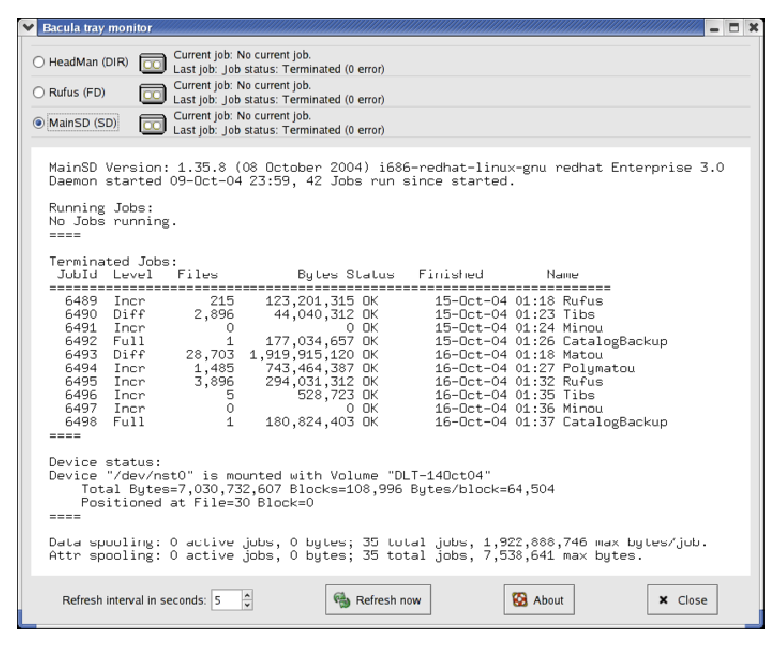
\includegraphics{./Bacula-tray-monitor.eps} 

L'image montre le tray-monitor configur\'e pour trois {\it daemons}. En
cliquant sur les boutons radio dans le coin en haut \`a gauche de l'image,
vous pouvez voir l'\'etat de chacun des {\it daemons}. L'image montre l'\'etat
du Storage Daemon (MainSD) s\'electionn\'e. 

Le fichier de configuration du Monitor se trouve dans le r\'epertoire
sp\'ecifi\'e au niveau de l'option {\bf \verb{--{sysconfdir} de la commande {\bf
./configure} et se nomme par d\'efaut {\bf tray-monitor.conf}. En principe,
pour les nouveaux utilisateurs, il suffit de changer les permissions de ce
fichier pour permettre aux utilisateurs non-root d'ex\'ecuter le Monitor, en
effet cette application doit \^etre ex\'ecut\'e par le m\^eme utilisateur que
l'environnement graphique (n'oubliez pas de donner aux non-root le droit
d'ex\'ecuter {\bf bacula-tray-monitor}). Ceci ne constitue pas une faille de
s\'ecurit\'e tant que vous utilisez les r\'eglages par d\'efaut. 

\subsection{
\ilink{Configurer le File Daemon}{_ChapterStart25}}
\index[general]{Configurer le File Daemon }
\index[general]{Daemon!Configurer le File }
\addcontentsline{toc}{subsection}{Configurer le File Daemon}

Le File Daemon, est le programme qui s'ex\'ecute sur chaque machine cliente. A
la demande du Director, il d\'etermine les fichiers \`a sauvegarder et les
exp\'edie au Storage Daemon. 

Le fichier de configuration du File Daemon se trouve dans le r\'epertoire
sp\'ecifi\'e au niveau de l'option {\bf \verb{--{sysconfdir} de la commande {\bf
./configure} et se nomme par d\'efaut {\bf bacula-fd.conf}. Normalement, pour
les nouveaux utilisateurs, aucune modification n'est requise pour ce fichier.
Les r\'eglages par d\'efaut sont raisonnables. Cependant, si vous envisagez de
sauvegarder plus d'une machine, il vous faudra installer le File Daemon avec
un fichier de configuration sp\'ecifique sur chaque machine \`a sauvegarder.
Les informations concernant chaque File Daemon doivent appara{\^\i}tre dans le
fichier de configuration du Director. 

\subsection{
\ilink{Configurer le Director}{_ChapterStart40}}
\index[general]{Director!Configurer le }
\index[general]{Configurer le Director }
\addcontentsline{toc}{subsection}{Configurer le Director}

Le director est le programme central qui contr\^ole tous les autres {\it
daemons}. Il planifie et surveille les jobs \`a ex\'ecuter. 

Le fichier de configuration du Director se trouve dans le r\'epertoire
sp\'ecifi\'e au niveau de l'option {\bf \verb{--{sysconfdir} de la commande {\bf
./configure} et se nomme par d\'efaut {\bf bacula-dir.conf}. 

En g\'en\'eral, la seule modification n\'ecessaire consiste \`a faire en sorte
que la directive {\bf Include} de la Ressource FileSet contienne au moins une
ligne avec un nom de fichier ou de r\'epertoire valide \`a sauvegarder. 

Si vous ne poss\'edez pas de lecteur DLT, vous voudrez probablement modifier
la ressource Storage pour donner un nom plus repr\'esentatif de votre
p\'eriph\'erique de stockage. Vous pouvez toujours utiliser les noms existants
puisque vous \^etes libre de les assigner arbitrairement, mais ils doivent
s'accorder avec les noms correspondants dans le fichier de configuration du
Storage Daemon. 

Vous pouvez aussi changer l'adresse \'electronique pour les notifications vers
votre propre adresse e-mail plut\^ot que vers celle de {\bf root}
(configuration par d\'efaut). 

Enfin, si vous avez plusieurs syst\`emes \`a sauvegarder, il vous faudra
sp\'ecifier un File Daemon (ou client) pour chaque syst\`eme sauvegard\'e,
pr\'ecisant ses nom, adresse et mot de passe. Nous estimons que baptiser vos
{\it daemons} du nom de vos syst\`emes suffix\'es avec {\bf -fd} aide beaucoup
\`a corriger les erreurs. Ainsi, si votre syst\`eme est {\bf foobaz}, vous
nommerez le {\it daemon} {\bf foobaz-fd}. Pour le Director, vous pourriez
utiliser {\bf foobaz-dir}, et {\bf foobaz-sd} pour le Storage Daemon. 
Chacun de vos composants de Bacula {\bf doit} avoir un nom unique 
Si vous les nommez tous \`a l'identique, en plus de ne jamais savoir 
quel {\it daemon} envoie quel message, s'ils partagent le m\^eme r\'epertoire 
de travail (working directory), les noms de fichiers temporaires des {\it daemons} 
ne seront pas uniques et vous aurez d'\'etranges erreurs.

\subsection{
\ilink{Configurer le Storage Daemon}{_ChapterStart31}}
\index[general]{Daemon!Configurer le Storage }
\index[general]{Configurer le Storage Daemon }
\addcontentsline{toc}{subsection}{Configurer le Storage Daemon}

Le Storage Daemon est responsable, sur demande du Director, de la r\'eception
des donn\'ees en provenance des File Daemons, et de leur \'ecriture sur le
medium de stockage, ou, dans le cas d'une restauration, de trouver les
donn\'ees pour les envoyer vers le File Daemon. 

Le fichier de configuration du Storage Daemon se trouve dans le r\'epertoire
sp\'ecifi\'e au niveau de l'option {\bf \verb{--{sysconfdir} de la commande {\bf
./configure} et se nomme par d\'efaut {\bf bacula-sd.conf}. Modifiez ce
fichier pour accorder les noms de p\'eriph\'eriques de stockage \`a ceux que
vous poss\'edez. Si le processus d'installation a convenablement d\'etect\'e
votre syst\`eme, elles seront d\'ej\`a correctement r\'egl\'ees. Ces
ressources de stockage "Name" et "Media Type" doivent \^etre les m\^emes
que leurs correspondantes du fichier de configuration du Director {\bf
bacula-dir.conf}. Si vous souhaitez sauvegarder vers un fichier plut\^ot que
sur des bandes, la ressource Device doit pointer vers un r\'epertoire o\`u des
fichiers seront cr\'e\'es en guise de Volumes lorque vous \'etiquetterez
(label) vos Volumes. 
\label{ConfigTesting}

\section{Tester vos Fichiers de Configuration}
\index[general]{Configuration!Tester vos Fichiers de }
\index[general]{Tester vos Fichiers de Configuration }
\addcontentsline{toc}{section}{Tester vos Fichiers de Configuration}

Vous pouvez tester la validit\'e syntaxique de vos fichiers de configuration,
afficher tout message d'erreur et terminer. Par exemple, en supposant que vous
avez install\'e vos binaires et fichiers de configuration dans le m\^eme
r\'epertoire, 

\footnotesize
\begin{verbatim}
cd <installation-directory>
./bacula-dir -t -c bacula-dir.conf
./bacula-fd -t -c bacula-fd.conf
./bacula-sd -t -c bacula-sd.conf
./bconsole -t -c bconsole.conf
./gnome-console -t -c gnome-console.conf
./bwx-console -t -c wx-console.conf
su <normal user> -c "./bacula-tray-monitor -t -c tray-monitor.conf"
\end{verbatim}
\normalsize

testera le fichier de configuration de chacun des principaux programmes. Si le
fichier de configuration est correct, le programme se termine
sans rien afficher. Veuillez noter que selon les options de configuration que
vous avez choisies, il se peut qu'aucune des commandes ci-dessus ne soit
valable sur votre syst\`eme. Si vous avez install\'e les binaires dans les
r\'epertoires traditionnels d'Unix plut\^ot que dans un simple r\'epertoire,
il vous faudra modifier les commandes ci-dessus en cons\'equence (pas de
"./" devant les commandes, et un chemin devant les fichiers de
configuration). 
\label{TapeTesting}

\section{Tester la compatibilit\'e de Bacula avec votre lecteur de bandes}
\index[general]{Tester la compatibilit\'e de Bacula avec votre lecteur de
bandes }
\index[general]{Bandes!Tester la compatibilit\'e de Bacula avec votre lecteur
de }
\addcontentsline{toc}{section}{Tester la compatibilit\'e de Bacula avec
votre lecteur de bandes}

Avant de gaspiller votre temps avec Bacula pour finalement constater qu'il ne
fonctionne pas avec votre lecteur de bandes, veuillez s'il vous pla\^it lire le
chapitre 
\ilink{btape -- Tester votre lecteur de bandes}{_ChapterStart27}
de ce manuel. Si vous poss\'edez un lecteur standard SCSI moderne sur un Linux
ou un Solaris, fort probablement, il fonctionnera, mais mieux vaut tester que
d'\^etre d\'e\c{c}u. Pour FreeBSD (et probablement les autres xBSD), la
lecture du chapitre mentionn\'e ci-dessus est un devoir. Pour FreeBSD,
consultez aussi 
\elink{The FreeBSD Diary}{http://www.freebsddiary.org/bacula.php} pour une
description d\'etaill\'ee de la m\'ethode pour faire fonctionner Bacula sur
votre syst\`eme. De plus, les utilisateurs de versions de FreeBSD
ant\'erieures \`a 4.9-STABLE dat\'ee du lundi 29 d\'ecembre 2003 15:18:01 UTC
qui pr\'evoient d'utiliser des lecteurs de bandes sont invit\'es \`a lire le
fichier {\bf platforms/freebsd/pthreads-fix.txt} du r\'epertoire principal de
Bacula, qui contient d'importantes informations sur la compatibilit\'e de
Bacula avec leur syst\`eme. 
\label{notls}

\section{D\'ebarrassez-vous du r\'epertoire /lib/tls}
\index[general]{D\'ebarrassez-vous du r\'epertoire /lib/tls }
\addcontentsline{toc}{section}{D\'ebarrassez-vous du r\'epertoire /lib/tls}

La nouvelle librairie pthreads {\bf /lib/tls} install\'ee par d\'efaut sur les
syst\`emes Red Hat r\'ecents (kernels 2.4.x) est d\'efectueuse. Vous devez la
supprimer ou la renommer, puis rebooter votre syst\`eme avant d'ex\'ecuter
Bacula, faute de quoi, apr\`es environ une semaine de fonctionnement, Bacula
se bloquera pour de longues p\'eriodes, voire d\'efinitivement. Veuillez consulter 
le chapitre \ilink{Syst\`emes support\'es}{SupportedOSes} pour plus
d'informations sur ce probl\`eme. 

Ce probl\`eme n'existe plus avec les noyaux 2.6.

\label{Running1}

\section{Ex\'ecuter Bacula}
\index[general]{Bacula!Ex\'ecuter }
\index[general]{Ex\'ecuter Bacula }
\addcontentsline{toc}{section}{Ex\'ecuter Bacula}

La partie la plus importante de l'ex\'ecution de Bacula est probablement la
capacit\'e de restaurer les fichiers. Si vous n'avez pas essay\'e de
r\'ecup\'erer des fichiers au moins une fois, vous subirez une bien plus forte
pression le jour o\`u vous devrez r\'eellement le faire, et serez enclin \`a
commettre des erreurs que vous n'auriez pas commises si vous aviez d\'ej\`a
essay\'e. 

Pour avoir rapidement une bonne id\'ee de la fa\c{c}on d'utiliser Bacula,
nous vous recommandons {\bf fortement} de suivre les exemples du 
\ilink{chapitre ex\'ecuter Bacula}{_ChapterStart1} de ce manuel,
o\`u vous trouverez des informations d\'etaill\'ees sur l'ex\'ecution de
Bacula. 

\section{Rotation des logs}
\index[general]{Logs!Rotation des }
\index[general]{Rotation des logs }
\addcontentsline{toc}{section}{Rotation des logs}

Si vous utilisez le {\bf bacula-dir.conf} par d\'efaut ou une variante, vous
constaterez qu'il r\'ecup\`ere toutes les sorties de Bacula dans un fichier.
Pour \'eviter que ce fichier ne croisse sans limites, nous vous recommandons
de copier le fichier {\bf logrotate} depuis {\bf scripts/logrotate} vers {\bf
/etc/logrotate.d/bacula}. Ainsi les fichiers de logs subiront une rotation
mensuelle et seront conserv\'es pour une dur\'ee maximum de cinq mois. Vous
pouvez \'editer ce fichier pour adapter la rotation \`a votre convenance. 

\section{Log Watch}
\index[general]{Watch!Log}
\index[general]{Log Watch}
\addcontentsline{toc}{section}{Log Watch}
Certains syst\`emes tels que RedHat et Fedora ex\'ecutent le programme 
logwatch chaque nuit pour analyser vos fichiers de log et vous 
envoyer un rapport par mail. Si vous souhaitez inclure la sortie 
de vos jobs Bacula dans ce rapport, veuillez regarder dans le r\'epertoire  
{\bf scripts/logwatch}. Le fichier {\bf README} fournit une br\`eve 
explication sur la fa\c {c}on d'installer le script, et quelle genre 
de r\'esultats en attendre.

\section{Reprise d'activit\'e apr\`es un d\'esastre (disaster recovery)}
\index[general]{Recovery!Reprise d'activit\'e apr\`es un d\'esastre disaster }
\index[general]{Reprise d'activit\'e apr\`es un d\'esastre (disaster recovery)
}
\addcontentsline{toc}{section}{Reprise d'activit\'e apr\`es un d\'esastre
(disaster recovery)}

Si vous avez l'intention d'utiliser Bacula en tant qu'outil de disaster
recovery plut\^ot que comme un simple programme pour restaurer les fichiers
perdus, vous serez int\'eress\'e par le 
\ilink{chapitre Plan de reprise d'activit\'e avec
Bacula}{_ChapterStart38} de ce manuel. 

De toute fa\c{c}on, vous \^etes fortement invit\'e \`a tester soigneusement
la restauration de quelques fichiers que vous aurez pr\'ealablement
sauvegard\'es, plut\^ot que d'attendre qu'un d\'esastre ne frappe. Ainsi, vous
serez pr\'epar\'e. 
   % install



%%
%%

\chapter{Tutorial}
\label{TutorialChapter}
\index[general]{Tutorial}

This chapter will guide you through running Bareos. To do so, we assume you
have installed Bareos.
However, we assume that you have not changed the .conf files. If you have
modified the .conf files, please go back and uninstall Bareos, then reinstall
it, but do not make any changes. The examples in this chapter use the default
configuration files, and will write the volumes to disk in your \path|/var/lib/bareos/storage/|
directory, in addition, the data backed up will be the source directory where
you built Bareos. As a consequence, you can run all the Bareos daemons for
these tests as non-root. Please note, in production, your File daemon(s) must
run as root. See the Security chapter for more information on this subject.

The general flow of running Bareos is:

\begin{enumerate}
\item Start the Database (if using MySQL or PostgreSQL)
\item Start the Bareos Daemons
\item Start the Console program to interact with the Director
\item Run a job
\item When the Volume fills, unmount the Volume, if it is a  tape, label a new
   one, and continue running. In this  chapter, we will write only to disk files
   so you won't  need to worry about tapes for the moment.
\item Test recovering some files from the Volume just written to  ensure the
   backup is good and that you know how to recover.  Better test before disaster
   strikes
\item Add a second client.
   \end{enumerate}

Each of these steps is described in more detail below.


\section{Installing Bareos}

For installing Bareos, follow the instructions from the \ilink{Installing Bareos}{InstallChapter} chapter.

% \section{Before Running Bareos}
% \index[general]{Bareos!Before Running}
% 
% Before running Bareos for the first time in production, we recommend that you
% run the {\bf test} command in the {\bf btape} program as described in the
% \ilink{Utility Program Chapter}{btape} of this manual. This will
% help ensure that Bareos functions correctly with your tape drive. If you have
% a modern HP, Sony, Tandberg Data or Quantum LTO tape drive running on Linux or
% Solaris, you can probably skip this test as Bareos is well tested with these
% drives and systems. For all other cases, you are {\bf strongly} encouraged to
% run the test before continuing. {\bf btape} also has a {\bf fill} command that
% attempts to duplicate what Bareos does when filling a tape and writing on the
% next tape. You should consider trying this command as well, but be forewarned,
% it can take hours (about four hours on my drive) to fill a large capacity tape.

\section{Starting the Database}

If you are using MySQL or PostgreSQL as the Bareos database, you should start
it before you attempt to run a job to avoid getting error messages from Bareos
when it starts.
If you are using SQLite you need do nothing. SQLite is automatically
started by {\bf Bareos}.

\section{Starting the Daemons}
\label{StartDaemon}
\index[general]{Starting the Daemons}
\index[general]{Daemon!Start}

Assuming you have installed the packages,
to start the three daemons, from your installation directory, simply enter:

\begin{verbatim}
service bareos-dir start
service bareos-sd start
service bareos-fd start
\end{verbatim}

The {\bf bareos} script starts the Storage daemon, the File daemon, and the
Director daemon, which all normally run as daemons in the background. If you
are using the autostart feature of Bareos, your daemons will either be
automatically started on reboot, or you can control them individually with the
files {\bf bareos-dir}, {\bf bareos-fd}, and {\bf bareos-sd}, which are
usually located in {\bf /etc/init.d}, though the actual location is system
dependent.
Some distributions may do this differently.

Note, on Windows, currently only the File daemon is ported, and it must be
started differently. Please see the
\ilink{Windows Version of Bareos}{Win32Chapter} chapter of this
manual.

The rpm packages configure the daemons to run as user=root and group=bareos.
The rpm installation also creates the group \group{bareos} if it does not exist on the
system. Any users that you add to the group \group{bareos} will have access to files
created by the daemons. To disable or alter this behavior edit the daemon
startup scripts:

\begin{itemize}
\item /etc/init.d/bareos-dir
\item /etc/init.d/bareos-sd
\item /etc/init.d/bareos-fd
\end{itemize}

and then restart as noted above.

The
\ilink{installation chapter}{InstallChapter} of this manual
explains how you can install scripts that will automatically restart the
daemons when the system starts.

\section{Using the Director to Query and Start Jobs}

To communicate with the director and to query the state of Bareos or run jobs,
from the top level directory, simply enter:

\command{bconsole}

For simplicity, here we will describe only the \command{bconsole} program,
also there is also a graphical interface called \command{BAT}.

The {\bf bconsole} runs the Bareos Console program, which connects to the
Director daemon. Since Bareos is a network program, you can run the Console
program anywhere on your network. Most frequently, however, one runs it on the
same machine as the Director. Normally, the Console program will print
something similar to the following:

\begin{commands}{bconsole}
<command>bconsole</command>
Connecting to Director bareos:9101
Enter a period to cancel a command.
*
\end{commands}

the asterisk is the console command prompt.

Type {\bf help} to see a list of available commands:

\begin{bconsole}{help}
* <input>help</input>
  Command       Description
  =======       ===========
  add           Add media to a pool
  autodisplay   Autodisplay console messages
  automount     Automount after label
  cancel        Cancel a job
  create        Create DB Pool from resource
  delete        Delete volume, pool or job
  disable       Disable a job
  enable        Enable a job
  estimate      Performs FileSet estimate, listing gives full listing
  exit          Terminate Bconsole session
  export        Export volumes from normal slots to import/export slots
  gui           Non-interactive gui mode
  help          Print help on specific command
  import        Import volumes from import/export slots to normal slots
  label         Label a tape
  list          List objects from catalog
  llist         Full or long list like list command
  messages      Display pending messages
  memory        Print current memory usage
  mount         Mount storage
  move          Move slots in an autochanger
  prune         Prune expired records from catalog
  purge         Purge records from catalog
  quit          Terminate Bconsole session
  query         Query catalog
  restore       Restore files
  relabel       Relabel a tape
  release       Release storage
  reload        Reload conf file
  rerun         Rerun a job
  run           Run a job
  status        Report status
  setbandwidth  Sets bandwidth
  setdebug      Sets debug level
  setip         Sets new client address -- if authorized
  show          Show resource records
  sqlquery      Use SQL to query catalog
  time          Print current time
  trace         Turn on/off trace to file
  unmount       Unmount storage
  umount        Umount - for old-time Unix guys, see unmount
  update        Update volume, pool or stats
  use           Use specific catalog
  var           Does variable expansion
  version       Print Director version
  wait          Wait until no jobs are running
\end{bconsole}

Details of the console program's commands are explained in the
\nameref{sec:bconsole} chapter.

\section{Running a Job}
\label{Running}
\index[general]{Job!Running a}
\index[general]{Running a Job}

At this point, we assume you have done the following:

\begin{itemize}
\item Installed Bareos
\item Started the Database
\item Prepared the database for Bareos
\item Started Bareos Director, Storage Daemon and File Daemon
\item Invoked the Console program with {\bf bconsole}
\end{itemize}

Furthermore, we assume for the moment you are using the default configuration
files.

At this point, enter the \bcommand{show filesets}{} and you should get something similar this:

\begin{bconsole}{show filesets}
* <input>show filesets</input>
FileSet: name=Full Set
      O M
      N
      I /usr/sbin
      N
      E /var/lib/bareos
      E /var/lib/bareos/storage
      E /proc
      E /tmp
      E /.journal
      E /.fsck
      N
\end{bconsole}

This is a pre-defined {\bf FileSet} that will backup the Bareos source
directory. The actual directory names printed should correspond to your system
configuration. For testing purposes, we have chosen a directory of moderate
size (about 40 Megabytes) and complexity without being too big. The FileSet
{\bf Catalog} is used for backing up Bareos's catalog and is not of interest
to us for the moment. The {\bf I} entries are the files or directories that
will be included in the backup and the {\bf E} are those that will be
excluded, and the {\bf O} entries are the options specified for
the FileSet. You can change what is backed up by editing {\bf bareos-dir.conf}
and changing the {\bf File =} line in the {\bf FileSet} resource.

Now is the time to run your first backup job. We are going to backup your
Bareos source directory to a File Volume in your \path|/var/lib/bareos/storage/|
 directory just to show you how easy it is. Now enter:

\footnotesize
\begin{verbatim}
status dir
\end{verbatim}
\normalsize

and you should get the following output:

\footnotesize
\begin{verbatim}
bareos-dir Version: 13.2.0 (09 April 2013) x86_64-pc-linux-gnu debian Debian GNU/Linux 6.0 (squeeze)
Daemon started 23-May-13 13:17. Jobs: run=0, running=0 mode=0
 Heap: heap=270,336 smbytes=59,285 max_bytes=59,285 bufs=239 max_bufs=239

Scheduled Jobs:
Level          Type     Pri  Scheduled          Name               Volume
===================================================================================
Incremental    Backup    10  23-May-13 23:05    BackupClient1      testvol
Full           Backup    11  23-May-13 23:10    BackupCatalog      testvol
====

Running Jobs:
Console connected at 23-May-13 13:34
No Jobs running.
====
\end{verbatim}
\normalsize

where the times and the Director's name will be different according to your
setup. This shows that an Incremental job is scheduled to run for the Job {\bf
BackupClient1} at 1:05am and that at 1:10, a {\bf BackupCatalog} is scheduled to
run. Note, you should probably change the name {\bf BackupClient1} to be the name of
your machine, if not, when you add additional clients, it will be very
confusing.

Now enter:

\footnotesize
\begin{verbatim}
status client
\end{verbatim}
\normalsize

and you should get something like:

\footnotesize
\begin{verbatim}
Automatically selected Client: bareos-fd
Connecting to Client bareos-fd at bareos:9102

bareos-fd Version: 13.2.0 (09 April 2013)  x86_64-pc-linux-gnu debian Debian GNU/Linux 6.0 (squeeze)
Daemon started 23-May-13 13:17. Jobs: run=0 running=0.
 Heap: heap=135,168 smbytes=26,000 max_bytes=26,147 bufs=65 max_bufs=66
 Sizeof: boffset_t=8 size_t=8 debug=0 trace=0 bwlimit=0kB/s

Running Jobs:
Director connected at: 23-May-13 13:58
No Jobs running.
====
\end{verbatim}
\normalsize

In this case, the client is named {\bf bareos-fd} your name will be different,
but the line beginning with {\bf bareos-fd Version ...} is printed by your File
daemon, so we are now sure it is up and running.

Finally do the same for your Storage daemon with:

\footnotesize
\begin{verbatim}
status storage
\end{verbatim}
\normalsize

and you should get:

\footnotesize
\begin{verbatim}
Automatically selected Storage: File
Connecting to Storage daemon File at bareos:9103

bareos-sd Version: 13.2.0 (09 April 2013) x86_64-pc-linux-gnu debian Debian GNU/Linux 6.0 (squeeze)
Daemon started 23-May-13 13:17. Jobs: run=0, running=0.
 Heap: heap=241,664 smbytes=28,574 max_bytes=88,969 bufs=73 max_bufs=74
 Sizes: boffset_t=8 size_t=8 int32_t=4 int64_t=8 mode=0 bwlimit=0kB/s

Running Jobs:
No Jobs running.
====

Device status:

Device "FileStorage" (/var/lib/bareos/storage) is not open.
==
====

Used Volume status:
====

====

\end{verbatim}
\normalsize

You will notice that the default Storage daemon device is named {\bf File} and
that it will use device {\bf /var/lib/bareos/storage}, which is not currently open.

Now, let's actually run a job with:

\footnotesize
\begin{verbatim}
run
\end{verbatim}
\normalsize

you should get the following output:

\footnotesize
\begin{verbatim}
Automatically selected Catalog: MyCatalog
Using Catalog "MyCatalog"
A job name must be specified.
The defined Job resources are:
     1: BackupClient1
     2: BackupCatalog
     3: RestoreFiles
Select Job resource (1-3):
\end{verbatim}
\normalsize

Here, Bareos has listed the three different Jobs that you can run, and you
should choose number {\bf 1} and type enter, at which point you will get:

\footnotesize
\begin{verbatim}
Run Backup job
JobName:  BackupClient1
Level:    Incremental
Client:   bareos-fd
Format:   Native
FileSet:  Full Set
Pool:     File (From Job resource)
NextPool: *None* (From unknown source)
Storage:  File (From Job resource)
When:     2013-05-23 14:50:04
Priority: 10
OK to run? (yes/mod/no):
\end{verbatim}
\normalsize

At this point, take some time to look carefully at what is printed and
understand it. It is asking you if it is OK to run a job named {\bf BackupClient1}
with FileSet {\bf Full Set} (we listed above) as an Incremental job on your
Client (your client name will be different), and to use Storage {\bf File} and
Pool {\bf Default}, and finally, it wants to run it now (the current time
should be displayed by your console).

Here we have the choice to run ({\bf yes}), to modify one or more of the above
parameters ({\bf mod}), or to not run the job ({\bf no}). Please enter {\bf
yes}, at which point you should immediately get the command prompt (an
asterisk). If you wait a few seconds, then enter the command {\bf messages}
you will get back something like:

\TODO{Replace bconsole output by current version of Bareos.}

\footnotesize
\begin{verbatim}
28-Apr-2003 14:22 bareos-dir: Last FULL backup time not found. Doing
                  FULL backup.
28-Apr-2003 14:22 bareos-dir: Start Backup JobId 1,
                  Job=Client1.2003-04-28_14.22.33
28-Apr-2003 14:22 bareos-sd: Job Client1.2003-04-28_14.22.33 waiting.
                  Cannot find any appendable volumes.
Please use the "label"  command to create a new Volume for:
    Storage:      FileStorage
    Media type:   File
    Pool:         Default
\end{verbatim}
\normalsize

The first message, indicates that no previous Full backup was done, so Bareos
is upgrading our Incremental job to a Full backup (this is normal). The second
message indicates that the job started with JobId 1., and the third message
tells us that Bareos cannot find any Volumes in the Pool for writing the
output. This is normal because we have not yet created (labeled) any Volumes.
Bareos indicates to you all the details of the volume it needs.

At this point, the job is BLOCKED waiting for a Volume. You can check this if
you want by doing a {\bf status dir}. In order to continue, we must create a
Volume that Bareos can write on. We do so with:

\footnotesize
\begin{verbatim}
label
\end{verbatim}
\normalsize

and Bareos will print:

\footnotesize
\begin{verbatim}
The defined Storage resources are:
     1: File
Item 1 selected automatically.
Enter new Volume name:
\end{verbatim}
\normalsize

at which point, you should enter some name beginning with a letter and
containing only letters and numbers (period, hyphen, and underscore) are also
permitted. For example, enter {\bf TestVolume001}, and you should get back:

\footnotesize
\begin{verbatim}
Defined Pools:
     1: Default
Item 1 selected automatically.
Connecting to Storage daemon File at bareos:8103 ...
Sending label command for Volume "TestVolume001" Slot 0 ...
3000 OK label. Volume=TestVolume001 Device=/var/lib/bareos/storage
Catalog record for Volume "TestVolume002", Slot 0  successfully created.
Requesting mount FileStorage ...
3001 OK mount. Device=/var/lib/bareos/storage
\end{verbatim}
\normalsize

Finally, enter {\bf messages} and you should get something like:

\footnotesize
\begin{verbatim}
28-Apr-2003 14:30 bareos-sd: Wrote label to prelabeled Volume
   "TestVolume001" on device /var/lib/bareos/storage
28-Apr-2003 14:30 rufus-dir: Bareos 1.30 (28Apr03): 28-Apr-2003 14:30
JobId:                  1
Job:                    BackupClient1.2003-04-28_14.22.33
FileSet:                Full Set
Backup Level:           Full
Client:                 bareos-fd
Start time:             28-Apr-2003 14:22
End time:               28-Apr-2003 14:30
Files Written:          1,444
Bytes Written:          38,988,877
Rate:                   81.2 KB/s
Software Compression:   None
Volume names(s):        TestVolume001
Volume Session Id:      1
Volume Session Time:    1051531381
Last Volume Bytes:      39,072,359
FD termination status:  OK
SD termination status:  OK
Termination:            Backup OK
28-Apr-2003 14:30 rufus-dir: Begin pruning Jobs.
28-Apr-2003 14:30 rufus-dir: No Jobs found to prune.
28-Apr-2003 14:30 rufus-dir: Begin pruning Files.
28-Apr-2003 14:30 rufus-dir: No Files found to prune.
28-Apr-2003 14:30 rufus-dir: End auto prune.
\end{verbatim}
\normalsize

If you don't see the output immediately, you can keep entering {\bf messages}
until the job terminates.

Instead of typing \command{messages} multiple times, 
you can also ask bconsole to wait, until a specific job is finished:
\footnotesize
\begin{verbatim}
wait jobid=1
\end{verbatim}
\normalsize
or just \command{wait}, which waits for all running jobs to finish.

Another useful command is {\bf autodisplay on}. 
With autodisplay activated, messages will automatically be displayed as soon as they are ready.

If you do an {\bf ls -l} of your {\bf /var/lib/bareos/storage} directory, you will see that you
have the following item:

\footnotesize
\begin{verbatim}
-rw-r-----    1 bareos bareos   39072153 Apr 28 14:30 TestVolume001
\end{verbatim}
\normalsize

This is the file Volume that you just wrote and it contains all the data of
the job just run. If you run additional jobs, they will be appended to this
Volume unless you specify otherwise.

You might ask yourself if you have to label all the Volumes that Bareos is
going to use. The answer for disk Volumes, like the one we used, is no. It is
possible to have Bareos automatically label volumes. For tape Volumes, you
will most likely have to label each of the Volumes you want to use.

If you would like to stop here, you can simply enter {\bf quit} in the Console
program.

% To clean up, simply
% delete the file {\bf /tmp/TestVolume001}, and you should also re-initialize
% your database using:
% 
% \footnotesize
% \begin{verbatim}
% ./drop_bareos_tables
% ./make_bareos_tables
% \end{verbatim}
% \normalsize
% 
% Please note that this will erase all information about the previous jobs that
% have run, and that you might want to do it now while testing but that normally
% you will not want to re-initialize your database.

If you would like to try restoring the files that you just backed up, read the
following section.
\label{restoring}

\section{Restoring Your Files}
\index[general]{Files!Restoring Your}
\index[general]{Restoring Your Files}

If you have run the default configuration and run the job as demonstrated above, 
you can restore the backed up files in the Console
program by entering:

\footnotesize
\begin{verbatim}
restore all
\end{verbatim}
\normalsize

where you will get:

\footnotesize
\begin{verbatim}
First you select one or more JobIds that contain files
to be restored. You will be presented several methods
of specifying the JobIds. Then you will be allowed to
select which files from those JobIds are to be restored.

To select the JobIds, you have the following choices:
     1: List last 20 Jobs run
     2: List Jobs where a given File is saved
     3: Enter list of comma separated JobIds to select
     4: Enter SQL list command
     5: Select the most recent backup for a client
     6: Select backup for a client before a specified time
     7: Enter a list of files to restore
     8: Enter a list of files to restore before a specified time
     9: Find the JobIds of the most recent backup for a client
    10: Find the JobIds for a backup for a client before a specified time
    11: Enter a list of directories to restore for found JobIds
    12: Select full restore to a specified Job date
    13: Cancel
Select item:  (1-13): 
\end{verbatim}
\normalsize

As you can see, there are a number of options, but for the current
demonstration, please enter {\bf 5} to do a restore of the last backup you
did, and you will get the following output:

\footnotesize
\begin{verbatim}
Automatically selected Client: bareos-fd
The defined FileSet resources are:
     1: Catalog
     2: Full Set
Select FileSet resource (1-2): 
\end{verbatim}
\normalsize

As you can see, Bareos knows what client
you have, and since there was only one, it selected it automatically.
Select {\bf 2}, because you want to restore files from the file set.

\footnotesize
\begin{verbatim}
+-------+-------+----------+------------+---------------------+---------------+
| jobid | level | jobfiles | jobbytes   | starttime           | volumename    |
+-------+-------+----------+------------+---------------------+---------------+
|     1 | F     |      166 | 19,069,526 | 2013-05-05 23:05:02 | TestVolume001 |
+-------+-------+----------+------------+---------------------+---------------+
You have selected the following JobIds: 1

Building directory tree for JobId(s) 1 ...  +++++++++++++++++++++++++++++++++++++++++
165 files inserted into the tree and marked for extraction.

You are now entering file selection mode where you add (mark) and
remove (unmark) files to be restored. No files are initially added, unless
you used the "all" keyword on the command line.
Enter "done" to leave this mode.

cwd is: /
$ 
\end{verbatim}
\normalsize

where I have truncated the listing on the right side to make it more readable.

Then Bareos produced a listing containing all the jobs that
form the current backup, in this case, there is only one, and the Storage
daemon was also automatically chosen. Bareos then took all the files that were
in Job number 1 and entered them into a {\bf directory tree} (a sort of in
memory representation of your filesystem). At this point, you can use the {\bf
cd} and {\bf ls} or {\bf dir} commands to walk up and down the directory tree
and view what files will be restored. For example, if I enter {\bf cd
/usr/sbin} and then enter {\bf dir} I will get a listing
of all the files in the Bareos source directory. On your system, the path might
be somewhat different. For more information on this, please refer to the
\ilink{Restore Command Chapter}{RestoreChapter} of this manual for
more details.

To exit this mode, simply enter:

\footnotesize
\begin{verbatim}
done
\end{verbatim}
\normalsize

and you will get the following output:

\footnotesize
\begin{verbatim}
Bootstrap records written to
   /home/user/bareos/testbin/working/restore.bsr
The restore job will require the following Volumes:

   TestVolume001
1444 files selected to restore.
Run Restore job
JobName:         RestoreFiles
Bootstrap:      /home/user/bareos/testbin/working/restore.bsr
Where:          /tmp/bareos-restores
Replace:        always
FileSet:        Full Set
Backup Client:  rufus-fd
Restore Client: rufus-fd
Storage:        File
JobId:          *None*
When:           2005-04-28 14:53:54
OK to run? (yes/mod/no):
Bootstrap records written to /var/lib/bareos/bareos-dir.restore.1.bsr

The job will require the following
   Volume(s)                 Storage(s)                SD Device(s)
===========================================================================
   
    TestVolume001             File                      FileStorage              

Volumes marked with "*" are online.


166 files selected to be restored.

Run Restore job
JobName:         RestoreFiles
Bootstrap:       /var/lib/bareos/bareos-dir.restore.1.bsr
Where:           /tmp/bareos-restores
Replace:         Always
FileSet:         Full Set
Backup Client:   bareos-fd
Restore Client:  bareos-fd
Format:          Native
Storage:         File
When:            2013-05-23 15:56:53
Catalog:         MyCatalog
Priority:        10
Plugin Options:  *None*
OK to run? (yes/mod/no): 
\end{verbatim}
\normalsize

If you answer {\bf yes} your files will be restored to {\bf
/tmp/bareos-restores}. If you want to restore the files to their original
locations, you must use the {\bf mod} option and explicitly set {\bf Where:}
to nothing (or to /). We recommend you go ahead and answer {\bf yes} and after
a brief moment, enter {\bf messages}, at which point you should get a listing
of all the files that were restored as well as a summary of the job that looks
similar to this:

\footnotesize
\begin{verbatim}
23-May 15:24 bareos-dir JobId 2: Start Restore Job RestoreFiles.2013-05-23_15.24.01_10
23-May 15:24 bareos-dir JobId 2: Using Device "FileStorage" to read.
23-May 15:24 bareos-sd JobId 2: Ready to read from volume "TestVolume001" on device "FileStorage" (/var/lib/bareos/storage).
23-May 15:24 bareos-sd JobId 2: Forward spacing Volume "TestVolume001" to file:block 0:194.
23-May 15:58 bareos-dir JobId 3: Bareos bareos-dir 13.2.0 (09Apr13):
  Build OS:               x86_64-pc-linux-gnu debian Debian GNU/Linux 6.0 (squeeze)
  JobId:                  2
  Job:                    RestoreFiles.2013-05-23_15.58.48_11
  Restore Client:         bareos-fd
  Start time:             23-May-2013 15:58:50
  End time:               23-May-2013 15:58:52
  Files Expected:         166
  Files Restored:         166
  Bytes Restored:         19,069,526
  Rate:                   9534.8 KB/s
  FD Errors:              0
  FD termination status:  OK
  SD termination status:  OK
  Termination:            Restore OK
\end{verbatim}
\normalsize

After exiting the Console program, you can examine the files in {\bf
/tmp/bareos-restores}, which will contain a small directory tree with all the
files. Be sure to clean up at the end with:

\footnotesize
\begin{verbatim}
rm -rf /tmp/bareos-restore
\end{verbatim}
\normalsize

\section{Quitting the Console Program}
\index[general]{Program!Quitting the Console}
\index[general]{Quitting the Console Program}

Simply enter the command {\bf quit}.
\label{SecondClient}

\section{Adding a Second Client}
\index[general]{Client!Adding a Second}
\index[general]{Adding a Second Client}

\subsection*{Changes on the Client}

If you have gotten the example shown above to work on your system, you may be
ready to add a second Client (File daemon). That is you have a second machine
that you would like backed up. The only part you need installed on the other
machine is the {\bf bareos-filedaemon}. 

This packages installs also its configuration file \path|/etc/bareos/bareos-fd.conf|
and sets its hostname + \path|-fd| as FileDaemon name.
However, the client does not known the Bareos Director, so this information must be given manually.

Lets assume, your second client has the hostname {\bf client2}
and this name is resolvable by DNS from the client and from the Bareos Director.

Specify the Bareos Director in the File Daemon configuration file \path|/etc/bareos/bareos-fd.conf|:

\footnotesize
\begin{verbatim}
...
#
# List Directors who are permitted to contact this File daemon
#
Director {
  Name = bareos-dir
  Password = "PASSWORD" # this is the passwort which you need to use within the client resource.
}
...
\end{verbatim}
\normalsize

The password is also generated at installation time,
but you are free to change it. Just keep in mind, it must be identical on the client and the Bareos Director.

Restart the Bareos File Daemon by
\footnotesize
\begin{verbatim}
root@client2:~ # service bareos-fd restart
\end{verbatim}
\normalsize



\subsection*{Changes on the Server (Bareos Director)}

Then you need to
make some additions to your Director's configuration file to define the new
File Daemon (Client).

 Starting from our original example which should be
installed on your system, you should add the following lines (essentially
copies of the existing data but with the names changed) to your Director's
configuration file {\bf bareos-dir.conf}.

Add following section makes the new client know to the Bareos Director. 
Add this section to the existing Bareos Director configuration file \path|/etc/bareos/bareos-dir.conf|:

\footnotesize
\begin{verbatim}
Client {
  Name = client2-fd
  Address = client2             # the name has to be resolvable through DNS. If this is not possible,
                                # you can work with IP addresses
  Password = "PASSWORD"         # password for FileDaemon which has to be the same like the password
                                # in the director resource of the bareos-fd.conf on the backup client.
                                # Copy it the the client to this line.
}
\end{verbatim}
\normalsize

Using this, the client is known to the Bareos Director. Additional you must specify, what to do with this client.
Therefore we specify a Job, which mostly takes its settings from the existing DefaultJob:

\footnotesize
\begin{verbatim}
Job {
  JobDefs = "DefaultJob"
  Name    = "client2"
  Client  = "client2-fd"
}
\end{verbatim}
\normalsize

Check if the configuration file is correct by
\footnotesize
\begin{verbatim}
root@bareos:~ # bareos-dir -t -c /etc/bareos/bareos-dir.conf
\end{verbatim}
\normalsize

If everything is okay, reload the Bareos Director:
\footnotesize
\begin{verbatim}
root@bareos:~ # service bareos-dir reload
\end{verbatim}
\normalsize

Now the setup for the second client should be ready.

To test the functionality, you can run a backup and restore job like in the example with the first attached FileDaemon.
However, there is an even earier way to check if a connection to a File Daemon is working. This is the \command{estimate listing} command in bconsole. Using this, the Bareos Director immediately connects to a client and returns all files that will be included in the next backup.

Start \command{bconsole} and follow the instructions:
\footnotesize
\begin{verbatim}
* estimate listing
\end{verbatim}
\normalsize

The result should appear immediately.

To make this a real production installation, you will possibly want to use
different Pool, or a different schedule. It is up to you to customize.

% For some important tips on changing names and passwords, and a diagram of what
% names and passwords must match, please see
% \ilink{Authorization Errors}{AuthorizationErrors} in the FAQ chapter
% of this manual.

\section{When The Tape Fills}
\label{FullTape}
\index[general]{Tape!Full}
\index[general]{When The Tape Fills}
\index[general]{Problem!Tape Full}

If you have scheduled your job, typically nightly, there will come a time when
the tape fills up and {\bf Bareos} cannot continue. In this case, Bareos will
send you a message similar to the following:

\footnotesize
\begin{verbatim}
bareos-sd: block.c:337 === Write error errno=28: ERR=No space left on device
\end{verbatim}
\normalsize

This indicates that Bareos got a write error because the tape is full. Bareos
will then search the Pool specified for your Job looking for an appendable
volume. In the best of all cases, you will have properly set your Retention
Periods and you will have all your tapes marked to be Recycled, and {\bf
Bareos} will automatically recycle the tapes in your pool requesting and
overwriting old Volumes. For more information on recycling, please see the
\ilink{Recycling chapter}{RecyclingChapter} of this manual. If you
find that your Volumes were not properly recycled (usually because of a
configuration error), please see the
\ilink{Manually Recycling Volumes}{manualrecycling} section of
the Recycling chapter.

If like me, you have a very large set of Volumes and you label them with the
date the Volume was first writing, or you have not set up your Retention
periods, Bareos will not find a tape in the pool, and it will send you a
message similar to the following:

\footnotesize
\begin{verbatim}
bareos-sd: Job usersave.2002-09-19.10:50:48 waiting. Cannot find any
          appendable volumes.
Please use the "label"  command to create a new Volume for:
    Storage:      SDT-10000
    Media type:   DDS-4
    Pool:         Default
\end{verbatim}
\normalsize

Until you create a new Volume, this message will be repeated an hour later,
then two hours later, and so on doubling the interval each time up to a
maximum interval of one day.

The obvious question at this point is: What do I do now?

The answer is simple: first, using the Console program, close the tape drive
using the {\bf unmount} command. If you only have a single drive, it will be
automatically selected, otherwise, make sure you release the one specified on
the message (in this case {\bf STD-10000}).

Next, you remove the tape from the drive and insert a new blank tape. Note, on
some older tape drives, you may need to write an end of file mark ({\bf mt \
-f \ /dev/nst0 \ weof}) to prevent the drive from running away when Bareos
attempts to read the label.

Finally, you use the {\bf label} command in the Console to write a label to
the new Volume. The {\bf label} command will contact the Storage daemon to
write the software label, if it is successful, it will add the new Volume to
the Pool, then issue a {\bf mount} command to the Storage daemon. See the
previous sections of this chapter for more details on labeling tapes.

The result is that Bareos will continue the previous Job writing the backup to
the new Volume.

If you have a Pool of volumes and Bareos is cycling through them, instead of
the above message "Cannot find any appendable volumes.", Bareos may ask you
to mount a specific volume. In that case, you should attempt to do just that.
If you do not have the volume any more (for any of a number of reasons), you
can simply mount another volume from the same Pool, providing it is
appendable, and Bareos will use it. You can use the {\bf list volumes} command
in the console program to determine which volumes are appendable and which are
not.

If like me, you have your Volume retention periods set correctly, but you have
no more free Volumes, you can relabel and reuse a Volume as follows:

\begin{itemize}
\item Do a {\bf list volumes} in the Console and select the oldest  Volume for
   relabeling.
\item If you have setup your Retention periods correctly, the  Volume should
   have VolStatus {\bf Purged}.
\item If the VolStatus is not set to Purged, you will need to purge  the
   database of Jobs that are written on that Volume. Do so  by using the command
   {\bf purge jobs volume} in the Console.  If you have multiple Pools, you will
be prompted for the  Pool then enter the VolumeName (or MediaId) when
requested.
\item Then simply use the {\bf relabel} command to relabel the  Volume.
   \end{itemize}

To manually relabel the Volume use the following additional steps:

\begin{itemize}
\item To delete the Volume from the catalog use the {\bf delete volume}
   command in the Console and select the VolumeName (or MediaId) to be  deleted.

\item Use the {\bf unmount} command in the Console to unmount the  old tape.
\item Physically relabel the old Volume that you deleted so that it  can be
   reused.
\item Insert the old Volume in the tape drive.
\item From a command line do: {\bf mt \ -f \ /dev/st0 \ rewind} and  {\bf mt \
   -f \ /dev/st0 \ weof}, where you need to use the proper  tape drive name for
   your system in place of {\bf /dev/st0}.
\item Use the {\bf label} command in the Console to write a new  Bareos label
   on your tape.
\item Use the {\bf mount} command in the Console if it is not automatically
   done, so that Bareos starts using your newly labeled tape.
   \end{itemize}

\section{Other Useful Console Commands}
\index[general]{Console!Commands!Useful}

\begin{description}

\item [status dir]
   \index[general]{Console!Command!status dir}
   Print a status of all running jobs and jobs  scheduled in the next 24 hours.

\item [status]
   \index[general]{Console!Command!status}
   The console program will prompt you to select  a daemon type, then will
request the daemon's status.

\item [status jobid=nn]
   \index[general]{Console!Command!status jobid}
   Print a status of JobId nn if it is running.  The Storage daemon is contacted
and requested to print a current  status of the job as well.

\item [list pools]
   \index[general]{Console!Command!list pools}
   List the pools defined in the Catalog (normally  only Default is used).

\item [list media]
   \index[general]{Console!Command!list media}
   Lists all the media defined in the Catalog.

\item [list jobs]
   \index[general]{Console!Command!list jobs}
   Lists all jobs in the Catalog that have run.

\item [list jobid=nn]
   \index[general]{Console!Command!list jobid}
   Lists JobId nn from the Catalog.

\item [list jobtotals]
   \index[general]{Console!Command!list jobtotals}
   Lists totals for all jobs in the Catalog.

\item [list files jobid=nn]
   \index[general]{Console!Command!list files jobid}
   List the files that were saved for JobId nn.

\item [list jobmedia]
   \index[general]{Console!Command!list jobmedia}
   List the media information for each Job run.

\item [messages]
   \index[general]{Console!Command!messages}
   Prints any messages that have been directed to the console.

\item [unmount storage=storage-name]
   \index[general]{Console!Command!unmount storage}
   Unmounts the drive associated with the storage  device with the name {\bf
storage-name} if the drive is not currently being  used. This command is used
if you wish Bareos to free the drive so  that you can use it to label a tape.


\item [mount storage=storage-name]
   \index[general]{Console!Command!mount storage}
   Causes the drive associated with the  storage device to be mounted again. When
Bareos reaches the end of a volume and requests you to mount a  new volume,
you must issue this command after you have placed the  new volume in the
drive. In effect, it is the signal needed by  Bareos to know to start reading
or writing the new volume.

\item [quit]
   \index[general]{Console!Command!quit}
   Exit or quit the console program.
\end{description}

Most of the commands given above, with the exception of {\bf list}, will
prompt you for the necessary arguments if you simply enter the command name.


% \section{Debug Daemon Output}
% \index[general]{Debug!Daemon}
% \index[general]{Daemon!Debug}
%
% %\TODO{needs to be adapted}
%
% If you want debug output from the daemons as they are running, start the
% daemons from the install directory as follows:
% 
% \footnotesize
% \begin{verbatim}
% ./bareos start -d100
% \end{verbatim}
% \normalsize
% 
% This can be particularly helpful if your daemons do not start correctly,
% because direct daemon output to the console is normally directed to the
% NULL device, but with the debug level greater than zero, the output
% will be sent to the starting terminal.
% 
% To stop the three daemons, enter the following from the install directory:
% 
% \footnotesize
% \begin{verbatim}
% ./bareos stop
% \end{verbatim}
% \normalsize
% 
% The execution of {\bf bareos stop} may complain about pids not found. This is
% OK, especially if one of the daemons has died, which is very rare.
% 
% To do a full system save, each File daemon must be running as root so that it
% will have permission to access all the files. None of the other daemons
% require root privileges. However, the Storage daemon must be able to open the
% tape drives. On many systems, only root can access the tape drives. Either run
% the Storage daemon as root, or change the permissions on the tape devices to
% permit non-root access. MySQL and PostgreSQL can be installed and run with any
% userid; root privilege is not necessary.

\section{Patience When Starting Daemons or Mounting Blank Tapes}

When you start the Bareos daemons, the Storage daemon attempts to open all
defined storage devices and verify the currently mounted Volume (if
configured). Until all the storage devices are verified, the Storage daemon
will not accept connections from the Console program. If a tape was previously
used, it will be rewound, and on some devices this can take several minutes.
As a consequence, you may need to have a bit of patience when first contacting
the Storage daemon after starting the daemons. If you can see your tape drive,
once the lights stop flashing, the drive will be ready to be used.

The same considerations apply if you have just mounted a blank tape in a drive
such as an HP DLT. It can take a minute or two before the drive properly
recognizes that the tape is blank. If you attempt to {\bf mount} the tape with
the Console program during this recognition period, it is quite possible that
you will hang your SCSI driver (at least on my Red Hat Linux system). As a
consequence, you are again urged to have patience when inserting blank tapes.
Let the device settle down before attempting to access it.

\section{Difficulties Connecting from the FD to the SD}
\index[general]{Problem!Connecting from the FD to the SD}

If you are having difficulties getting one or more of your File daemons to
connect to the Storage daemon, it is most likely because you have not used a
fully qualified domain name on the {\bf Address} directive in the
Director's Storage resource. That is the resolver on the File daemon's machine
(not on the Director's) must be able to resolve the name you supply into an IP
address. An example of an address that is guaranteed not to work: {\bf
localhost}. An example that may work: {\bf megalon}. An example that is more
likely to work: {\bf magalon.mydomain.com}. On Win32 if you don't have a good
resolver (often true on older Windows systems), you might try using an IP
address in place of a name.

If your address is correct, then make sure that no other program is using the
port 9103 on the Storage daemon's machine. The Bacula project has reserved 
these port numbers by IANA, therefore they should only be used by Bacula and its replacements like Bareos.
However, apparently
some HP printers do use these port numbers. A {\bf netstat -a} on the Storage
daemon's machine can determine who is using the 9103 port (used for FD to SD
communications in Bareos).



\section{Creating a Pool}
\label{Pool}
\index[general]{Pool!Creating a}
\index[general]{Creating a Pool}

Creating the Pool is automatically done when {\bf Bareos} starts, so if you
understand Pools, you can skip to the next section.

When you run a job, one of the things that Bareos must know is what Volumes to
use to backup the FileSet. Instead of specifying a Volume (tape) directly, you
specify which Pool of Volumes you want Bareos to consult when it wants a tape
for writing backups. Bareos will select the first available Volume from the
Pool that is appropriate for the Storage device you have specified for the Job
being run. When a volume has filled up with data, {\bf Bareos} will change its
VolStatus from {\bf Append} to {\bf Full}, and then {\bf Bareos} will use the
next volume and so on. If no appendable Volume exists in the Pool, the
Director will attempt to recycle an old Volume, if there are still no
appendable Volumes available, {\bf Bareos} will send a message requesting the
operator to create an appropriate Volume.

{\bf Bareos} keeps track of the Pool name, the volumes contained in the Pool,
and a number of attributes of each of those Volumes.

When Bareos starts, it ensures that all Pool resource definitions have been
recorded in the catalog. You can verify this by entering:

\footnotesize
\begin{verbatim}
list pools
\end{verbatim}
\normalsize

to the console program, which should print something like the following:

\footnotesize
\begin{verbatim}
*list pools
Using default Catalog name=MySQL DB=bareos
+--------+---------+---------+---------+----------+-------------+
| PoolId | Name    | NumVols | MaxVols | PoolType | LabelFormat |
+--------+---------+---------+---------+----------+-------------+
| 1      | Default | 3       | 0       | Backup   | *           |
| 2      | File    | 12      | 12      | Backup   | File        |
+--------+---------+---------+---------+----------+-------------+
*
\end{verbatim}
\normalsize

If you attempt to create the same Pool name a second time, {\bf Bareos} will
print:

\footnotesize
\begin{verbatim}
Error: Pool Default already exists.
Once created, you may use the update command to
modify many of the values in the Pool record.
\end{verbatim}
\normalsize


\section{Labeling Your Volumes}
\index[general]{Volume!Label}
\index[general]{Labeling Your Volumes}
\label{Labeling}

Bareos requires that each Volume contains a software label. There are several
strategies for labeling volumes. The one I use is to label them as they are
needed by {\bf Bareos} using the console program. That is when Bareos needs a
new Volume, and it does not find one in the catalog, it will send me an email
message requesting that I add Volumes to the Pool. I then use the {\bf label}
command in the Console program to label a new Volume and to define it in the
Pool database, after which Bareos will begin writing on the new Volume.
Alternatively, I can use the Console {\bf relabel} command to relabel a Volume
that is no longer used providing it has VolStatus {\bf Purged}.

Another strategy is to label a set of volumes at the start, then use them as
{\bf Bareos} requests them. This is most often done if you are cycling through
a set of tapes, for example using an autochanger. For more details on
recycling, please see the
\ilink{Automatic Volume Recycling}{RecyclingChapter} chapter of
this manual.

If you run a Bareos job, and you have no labeled tapes in the Pool, Bareos
will inform you, and you can create them "on-the-fly" so to speak. In my
case, I label my tapes with the date, for example: {\bf DLT-18April02}. See
below for the details of using the {\bf label} command.

\subsection*{Labeling Volumes with the Console Program}
\index[general]{Labeling Volumes with the Console Program}
\index[general]{Console!Command!label}

Labeling volumes is normally done by using the console program.

\begin{enumerate}
\item bconsole
\item label
\end{enumerate}

If Bareos complains that you cannot label the tape because it is already
labeled, simply {\bf unmount} the tape using the {\bf unmount} command in the
console, then physically mount a blank tape and re-issue the {\bf label}
command.

Since the physical storage media is different for each device, the {\bf label}
command will provide you with a list of the defined Storage resources such as
the following:

\footnotesize
\begin{verbatim}
The defined Storage resources are:
     1: File
     2: 8mmDrive
     3: DLTDrive
     4: SDT-10000
Select Storage resource (1-4):
\end{verbatim}
\normalsize

At this point, you should have a blank tape in the drive corresponding to the
Storage resource that you select.

It will then ask you for the Volume name.

\footnotesize
\begin{verbatim}
Enter new Volume name:
\end{verbatim}
\normalsize

If Bareos complains:

\footnotesize
\begin{verbatim}
Media record for Volume xxxx already exists.
\end{verbatim}
\normalsize

It means that the volume name {\bf xxxx} that you entered already exists in
the Media database. You can list all the defined Media (Volumes) with the {\bf
list media} command. Note, the LastWritten column has been truncated for
proper printing.

\footnotesize
\begin{verbatim}
+---------------+---------+--------+----------------+-----/~/-+------------+-----+
| VolumeName    | MediaTyp| VolStat| VolBytes       | LastWri | VolReten   | Recy|
+---------------+---------+--------+----------------+---------+------------+-----+
| DLTVol0002    | DLT8000 | Purged | 56,128,042,217 | 2001-10 | 31,536,000 |   0 |
| DLT-07Oct2001 | DLT8000 | Full   | 56,172,030,586 | 2001-11 | 31,536,000 |   0 |
| DLT-08Nov2001 | DLT8000 | Full   | 55,691,684,216 | 2001-12 | 31,536,000 |   0 |
| DLT-01Dec2001 | DLT8000 | Full   | 55,162,215,866 | 2001-12 | 31,536,000 |   0 |
| DLT-28Dec2001 | DLT8000 | Full   | 57,888,007,042 | 2002-01 | 31,536,000 |   0 |
| DLT-20Jan2002 | DLT8000 | Full   | 57,003,507,308 | 2002-02 | 31,536,000 |   0 |
| DLT-16Feb2002 | DLT8000 | Full   | 55,772,630,824 | 2002-03 | 31,536,000 |   0 |
| DLT-12Mar2002 | DLT8000 | Full   | 50,666,320,453 | 1970-01 | 31,536,000 |   0 |
| DLT-27Mar2002 | DLT8000 | Full   | 57,592,952,309 | 2002-04 | 31,536,000 |   0 |
| DLT-15Apr2002 | DLT8000 | Full   | 57,190,864,185 | 2002-05 | 31,536,000 |   0 |
| DLT-04May2002 | DLT8000 | Full   | 60,486,677,724 | 2002-05 | 31,536,000 |   0 |
| DLT-26May02   | DLT8000 | Append |  1,336,699,620 | 2002-05 | 31,536,000 |   1 |
+---------------+---------+--------+----------------+-----/~/-+------------+-----+
\end{verbatim}
\normalsize

Once Bareos has verified that the volume does not already exist, it will
prompt you for the name of the Pool in which the Volume (tape) is to be
created.  If there is only one Pool (Default), it will be automatically
selected.

If the tape is successfully labeled, a Volume record will also be created in
the Pool. That is the Volume name and all its other attributes will appear
when you list the Pool. In addition, that Volume will be available for backup
if the MediaType matches what is requested by the Storage daemon.

When you labeled the tape, you answered very few questions about it --
principally the Volume name, and perhaps the Slot. However, a Volume record in
the catalog database (internally known as a Media record) contains quite a few
attributes. Most of these attributes will be filled in from the default values
that were defined in the Pool (i.e. the Pool holds most of the default
attributes used when creating a Volume).

It is also possible to add media to the pool without physically labeling the
Volumes. This can be done with the \bcommand{add}{} command. For more information,
please see the
\nameref{sec:bconsole} chapter.


%%
%%

\chapter{Critical Items to Implement Before Production}
\label{CriticalChapter}
\index[general]{Production!Critical Items to Implement Before}
\index[general]{Critical Items to Implement Before Production}

We recommend you take your time before implementing a production on a Bareos
backup system since Bareos is a rather complex program, and if you make a
mistake, you may suddenly find that you cannot restore your files in case
of a disaster.  This is especially true if you have not previously used a
major backup product.

If you follow the instructions in this chapter, you will have covered most of
the major problems that can occur. It goes without saying that if you ever
find that we have left out an important point, please inform us, so
that we can document it to the benefit of everyone.

\label{Critical}
\section{Critical Items}
\index[general]{Critical Items}

The following assumes that you have installed Bareos, you more or less
understand it, you have at least worked through the tutorial or have
equivalent experience, and that you have set up a basic production
configuration. If you haven't done the above, please do so and then come back
here. The following is a sort of checklist that points with perhaps a brief
explanation of why you should do it.  In most cases, you will find the
details elsewhere in the manual.  The order is more or less the order you
would use in setting up a production system (if you already are in
production, use the checklist anyway).

\begin{itemize}
\item Test your tape drive for compatibility with Bareos by using the test
   command of the \ilink{btape}{btape} program.
% TODO: missing chapter
% \item Better than doing the above is to walk through the nine steps in the
%    \ilink{Tape Testing}{TapeTestingChapter} chapter of the manual. It
%    may take you a bit of time, but it will eliminate surprises.
\item Test the end of tape handling of your tape drive by using the
   fill command in the \ilink{btape}{btape} program.
\item Do at least one restore of files. If you backup multiple OS types
   (Linux, Solaris, HP, MacOS, FreeBSD, Win32, ...),
   restore files from each system type. The
   \ilink{Restoring Files}{RestoreChapter} chapter shows you how.
\item Write a bootstrap file to a separate system for each backup job.
   See \linkResourceDirective{Dir}{Job}{Write Bootstrap} directive and more details are available in the
   \nameref{BootstrapChapter} chapter. Also, the default
   \file{bareos-dir.conf} comes with a Write Bootstrap directive defined. This  allows
   you to recover the state of your system as of the last backup.
\item Backup your catalog. An example of this is found in the default
   bareos-dir.conf file. The backup script is installed by default and
   should handle any database, though you may want to make your own local
   modifications.  See also \ilink{Backing Up Your Bareos Database}{BackingUpBareos} for more
   information.
\item Write a bootstrap file for the catalog. An example of this is found in
   the default bareos-dir.conf file. This will allow you to quickly restore your
   catalog in the event it is wiped out -- otherwise it  is many excruciating
   hours of work.
\item Make a copy of the bareos-dir.conf, bareos-sd.conf, and
   bareos-fd.conf files that you are using on your server. Put it in a safe
   place (on another machine) as these files can be difficult to
   reconstruct if your server dies.
% \item Make a Bareos Rescue CDROM! See the
%    \ilink{Disaster Recovery Using a Bareos Rescue
%    CDROM}{RescueChapter} chapter. It is trivial to  make such a CDROM,
%    and it can make system recovery in the event of  a lost hard disk infinitely
%    easier.
\item Bareos assumes all filenames are in UTF-8 format. This is important
   when saving the filenames to the catalog. For Win32 machine, Bareos will
   automatically convert from Unicode to UTF-8, but on Unix, Linux, *BSD,
   and MacOS X machines, you must explicitly ensure that your locale is set
   properly. Typically this means that the {\bf LANG} environment variable
   must end in {\bf .UTF-8}. A full example is {\bf en\_US.UTF-8}. The
   exact syntax may vary a bit from OS to OS, and exactly how you define it
   will also vary.

   On most modern Win32 machines, you can edit the conf files with {\bf
   notepad} and choose output encoding UTF-8.
\end{itemize}

\section{Recommended Items}
\index[general]{Recommended Items}

Although these items may not be critical, they are recommended and will help
you avoid problems.

\begin{itemize}
\item Read the \nameref{QuickStartChapter} chapter
\item After installing and experimenting with Bareos, read and work carefully
   through the examples in the
   \nameref{TutorialChapter} chapter  of this manual.
\item Learn what each of the \nameref{sec:Utilities}
   does.
\item Set up reasonable retention periods so that your catalog does not  grow
   to be too big. See the following three chapters:\\
   \nameref{RecyclingChapter},\\
   \nameref{DiskChapter},\\
   \nameref{PoolsChapter}.
% \item Perform a bare metal recovery using the Bareos Rescue CDROM.  See the
%    \ilink{Disaster Recovery Using a Bareos Rescue CDROM}{RescueChapter}
%     chapter.
\end{itemize}

If you absolutely must implement a system where you write a different
tape each night and take it offsite in the morning. We recommend that you do
several things:
\begin{itemize}
\item Write a bootstrap file of your backed up data and a bootstrap file
   of your catalog backup to a external media like CDROM or USB stick, and take that with
   the tape.  If this is not possible, try to write those files to another
   computer or offsite computer, or send them as email to a friend. If none
   of that is possible, at least print the bootstrap files and take that
   offsite with the tape.  Having the bootstrap files will make recovery
   much easier.
\item It is better not to force Bareos to load a particular tape each day.
   Instead, let Bareos choose the tape.  If you need to know what tape to
   mount, you can print a list of recycled and appendable tapes daily, and
   select any tape from that list.  Bareos may propose a particular tape
   for use that it considers optimal, but it will accept any valid tape
   from the correct pool.
\end{itemize}
     % install

\part{Configuration Files}

\chapter{Customizing the Configuration Files}
\label{ConfigureChapter}
\index[general]{Files!Customizing the Configuration}
\index[general]{Customizing the Configuration Files}

    \chapter{Customizing the Configuration}
\label{ConfigureChapter}
\index[general]{Customizing the Configuration}

Each Bareos component (Director, Client, Storage, Console) has its own configuration
containing a set of resource definitions. These resources are very
similar from one service to another, but may contain different directives
(records) depending on the component. For example, in the Director configuration,
the \nameref{DirectorResourceDirector} defines the name of the Director, a number
of global Director parameters and his password. In the File daemon
configuration, the \nameref{ClientResourceDirector} specifies which Directors are
permitted to use the File daemon.

If you install all Bareos daemons (Director, Storage and File Daemon) onto one system,
the Bareos package tries its best to generate a working configuration as a basis for your individual configuration.

The details of each resource and the directives permitted therein are
described in the following chapters.

The following configuration files must be present:

\begin{itemize}
\item
   \nameref{DirectorChapter} -- to define the resources
   necessary for the Director. You define all the Clients  and Storage daemons
   that you use in this configuration file.
\item
   \nameref{StoredConfChapter} -- to define the resources to
   be used by each Storage daemon. Normally, you will have a single Storage
   daemon that controls your disk storage or tape drives. However, if you have
   tape drives on several machines, you will have at least one Storage daemon
   per machine.
\item
   \nameref{FiledConfChapter} -- to define the resources for
   each client to be backed up. That is, you will have a separate  Client
   resource file on each machine that runs a File daemon.
\item
   \nameref{ConsoleConfChapter} -- to define the resources for
   the Console program (user interface to the Director).  It defines which
Directors are  available so that you may interact with them.
\end{itemize}


\section{Configuration Path Layout}
\index[general]{Configuration!Directories}
\index[general]{Configuration!Subdirectories}

When a Bareos component starts, it reads its configuration.
In Bareos $<$ 16.2.2 only configuration files (which optionally can include other files) are supported.
Since Bareos \sinceVersion{}{Configuration Subdirectories}{16.2.2} also configuration subdirectories are supported.

\subsubsection{Naming}

In this section, the following naming is used:

\begin{itemize}
    \item \path|$CONFIGDIR|\hide{$} refers to the base configuration directory.
        Bareos Linux packages use \configPathUnix.
    \item A component is one of the following Bareos programs:
    \begin{itemize}
        \item bareos-dir
        \item bareos-sd
        \item bareos-fd
        \item bareos-traymonitor
        \item bconsole
        \item bat (only legacy config file: bat.conf)
        \item Bareos tools, like \nameref{sec:VolumeUtilityCommands} and others.
    \end{itemize}
    \item \path|$COMPONENT|\hide{$} refers to one of the listed components.
%
%     \item Legacy config file (still fully supported, with some
%           limitation when using the configuration API):
%         \begin{itemize}
%             \item \path|$CONFIGDIR/$COMPONENT.conf|
%         \end{itemize}
\end{itemize}

\subsection{What configuration will be used?}
\label{sec:ConfigurationFileOrConfigurationSubDirectories}

When starting a Bareos component, it will look for its configuration.
Bareos components allow the configuration file/directory to be specified as a command line parameter \path|-c $PATH|\hide{$}.

\begin{itemize}
    \item configuration path parameter is not given (default)
        \begin{itemize}
        \item \path|$CONFIGDIR/$COMPONENT.conf| is a file
            \begin{itemize}
            \item the configuration is read from the file \path|$CONFIGDIR/$COMPONENT.conf|
            \end{itemize}
        \item \path|$CONFIGDIR/$COMPONENT.d/| is a directory
            \begin{itemize}
            \item the configuration is read from \path|$CONFIGDIR/$COMPONENT.d/*/*.conf| (subdirectory configuration)
            \end{itemize}
        \end{itemize}
    \item configuration path parameter is given (\path|-c $PATH|)
        \begin{itemize}
        \item \path|$PATH| is a file
            \begin{itemize}
            \item the configuration is read from the file specified in \path|$PATH|
            \end{itemize}
        \item \path|$PATH| is a directory
            \begin{itemize}
            \item the configuration is read from \path|$PATH/$COMPONENT.d/*/*.conf| (subdirectory configuration)
            \end{itemize}
        \end{itemize}
\end{itemize}

As the \path|$CONFIGDIR|\hide{$} differs between platforms or is overwritten by the path parameter,
the documentation will often refer to the configuration without the leading path
(e.g. \path|$COMPONENT.d/*/*.conf|\hide{$} instead of \path|$CONFIGDIR/$COMPONENT.d/*/*.conf|).

\begin{center}
\includegraphics[width=0.8\linewidth]{\idir bareos-read-configuration}
\end{center}


When subdirectory configuration is used,
all files matching \path|$PATH/$COMPONENT.d/*/*.conf| will be read, see \nameref{sec:ConfigurationSubdirectories}.

\paragraph{Relation between Bareos components and configuration}

\begin{center}
\begin{tabular}{ l || l | l }
Bareos component &
\shortstack[l]{Configuration File \\ (default path on Unix)} &
\shortstack[l]{Subdirectory Configuration Scheme\\ (default path on Unix) \\ since Bareos $>=$ 16.2.2} \\
\hline
\hline

bareos-dir                   & \file{bareos-dir.conf}       & \file{bareos-dir.d} \\
\nameref{DirectorChapter}    & (\configFileDirUnix)         & (\configDirectoryDirUnix) \\
\hline

bareos-sd                    & \file{bareos-sd.conf}        & \file{bareos-sd.d} \\
\nameref{StoredConfChapter}  & (\configFileSdUnix)          & (\configDirectorySdUnix) \\
\hline

bareos-fd                    & \file{bareos-fd.conf}        & \file{bareos-fd.d} \\
\nameref{FiledConfChapter}   & (\configFileFdUnix)          & (\configDirectoryFdUnix) \\
\hline

bconsole                     & \file{bconsole.conf}         & \file{bconsole.d} \\
\nameref{ConsoleConfChapter} & (\configFileBconsoleUnix)    & (\configDirectoryBconsoleUnix) \\
\hline

bareos-traymonitor           & \file{tray-monitor.conf}     & \file{tray-monitor.d} \\
\nameref{sec:MonitorConfig}  & (\configFileTrayMonitorUnix) & (\configDirectoryTrayMonitorUnix) \\
\hline

bat                          & \file{bat.conf}              & (not supported) \\
                             & ({\configFileBatUnix})       &  \\
\hline

\nameref{sec:VolumeUtilityCommands} & \file{bareos-sd.conf}        & \file{bareos-sd.d} \\
(use the bareos-sd configuration)   & (\configFileSdUnix)          & (\configDirectorySdUnix) \\

\end{tabular}
\end{center}



\subsection{Subdirectory Configuration Scheme}
\label{sec:SubdirectoryConfigurationScheme}
\label{sec:ConfigurationSubdirectories}
% ConfigurationIncludeDirectory is referenced from the Bareos code.
\label{ConfigurationIncludeDirectory}

If the subdirectory configuration is used, instead of a single configuration file,
all files matching \path|$COMPONENT.d/*/*.conf|\hide{$} are read as a configuration,
see \nameref{sec:ConfigurationFileOrConfigurationSubDirectories}.

\subsubsection{Reason for the Subdirectory Configuration Scheme}

In Bareos $<$ 16.2.2, Bareos uses one configuration file per component.

Most larger Bareos environments split their configuration into separate
files, making it easier to manage the configuration.

Also some extra packages (bareos-webui, plugins, ...) require a configuration,
which must be included into the \bareosDir or \bareosSd configuration.
The subdirectory approach makes it easier to add or modify the configuration resources of different Bareos packages.

The Bareos \ilink{configure}{sec:bcommandConfigure} command
requires a configuration directory structure, as provided by the subdirectory approach.

From Bareos \sinceVersion{}{Configuration subdirectories are used by default}{16.2.4} on,
new installations will use configuration subdirectories by default.


\subsubsection{Resource file conventions}
    \label{sec:ConfigurationResourceFileConventions}

\begin{itemize}
\item Each configuration resource has to use its own configuration file.
\item The path of a resource file is \path|$COMPONENT.d/$RESOURCETYPE/$RESOURCENAME.conf|.
\item The name of the configuration file is identical with the resource name:
    \begin{itemize}
    \item e.g.
        \begin{itemize}
        \item \path|bareos-dir.d/director/bareos-dir.conf|
        \item \path|bareos-dir.d/pool/Full.conf|
        \end{itemize}
    \item Exceptions:
        \begin{itemize}
        \item The resource file \path|bareos-fd.d/client/myself.conf| always has the file name \path|myself.conf|,
                while the name is normally set to the hostname of the system. 
        \end{itemize}
    \end{itemize}
\item Example resource files:
    \begin{itemize}
    \item Additional packages can contain configuration files that are automatically included. However, most additional configuration resources require configuration. When a resource file requires configuration, it has to be included as an example file:
        \begin{itemize}
        \item \path|$CONFIGDIR/$COMPONENT.d/$RESOURCE/$NAME.conf.example|
        \item For example, the \bareosWebui entails one config resource and one config resource example for the \bareosDir:
            \begin{itemize}
            \item \path|$CONFIGDIR/bareos-director.d/profile/webui-admin.conf|
            \item \path|$CONFIGDIR/bareos-director.d/console/admin.conf.example|\hide{$}
            \end{itemize}
        \end{itemize}
    \end{itemize}
\item \hypertarget{sec:deleteConfigurationResourceFiles}Disable/remove configuration resource files:
    \begin{itemize}
    \item Normally you should not remove resources that are already in use (jobs, clients, ...). Instead you should disable them by adding the directive \configline{Enable = no}. Otherwise you take the risk that orphaned entries are kept in the Bareos catalog. However, if a resource has not been used or all references have been cleared from the database, they can also be removed from the configuration.
    \warning{If you want to remove a configuration resource that is part of a Bareos package,
                    replace the resource configuration file by an empty file.
                    This prevents the resource from reappearing in the course of a package update.}
    \end{itemize}
\end{itemize}



\subsubsection{Using Subdirectories Configuration Scheme}

\paragraph{New installation}

\begin{itemize}
    \item The Subdirectories Configuration Scheme is used 
            by default from Bareos \sinceVersion{}{Subdirectories Configuration Scheme}{16.2.4} onwards.
    \item They will be usable immediately after installing a Bareos component.
    \item If additional packages entail example configuration files (\path|$NAME.conf.example|),
        copy them to \path|$NAME.conf|, modify it as required and reload or restart the component.
\end{itemize}

\paragraph{Updates from Bareos $<$ 16.2.4}
    \label{sec:UpdateToConfigurationSubdirectories}

\begin{itemize}
\item When updating to a Bareos version containing the Subdirectories Configuration,
            the existing configuration will not be touched and is still the default configuration.
    \begin{itemize}
    \item \warning{Problems can occur if you have implemented an own wildcard mechanism to load your configuration
            from the same subdirectories as used by the new packages (\path|$CONFIGDIR/$COMPONENT.d/*/*.conf|).
            In this case, newly installed configuration resource files can alter
            your current configuration by adding resources.}
            Best create a copy of your configuration directory before updating Bareos
            and modify your existing configuration file to use that other directory.
    \end{itemize}
\item As long as the old configuration file (\path|$CONFIGDIR/$COMPONENT.conf|) exists, it will be used.
\item The correct way of migrating to the new configuration scheme would be
            to split the configuration file into resources,
            store them in the resource directories and then remove the original configuration file.
    \begin{itemize}
    \item For migrating the \bareosDir configuration, the script \bareosMigrateConfigSh exists.
        Being called, it connects via \command{bconsole} to a running \bareosDir and creates subdirectories with the resource configuration files.
        \begin{commands}{\bareosMigrateConfigSh}
# prepare temporary directory
mkdir /tmp/baroes-dir.d
cd /tmp/baroes-dir.d

# download migration script
wget https://raw.githubusercontent.com/bareos/bareos-contrib/master/misc/bareos-migrate-config/bareos-migrate-config.sh

# execute the script
bash bareos-migrate-config.sh

# backup old configuration
mv /etc/bareos/bareos-dir.conf /etc/bareos/bareos-dir.conf.bak
mv /etc/bareos/bareos-dir.d /etc/bareos/bareos-dir.d.bak

# make sure, that all packaged configuration resources exists,
# otherwise they will be added when updating Bareos.
for i in `find  /etc/bareos/bareos-dir.d.bak/ -name *.conf -type f -printf "%P\n"`; do touch "$i"; done

# install newly generated configuration
cp -a /tmp/bareos-dir.d /etc/bareos/
        \end{commands}
        Restart the \bareosDir and verify your configuration.
        Also make sure, that all resource configuration files coming from Bareos packages exists, in doubt as empty files, see \hyperlink{sec:deleteConfigurationResourceFiles}{remove configuration resource files}.

    \item Another way, without splitting the configuration into resource files is:
        \begin{itemize}
        \item \begin{commands}{move configuration to subdirectory}
mkdir $CONFIGDIR/$COMPONENT.d/migrate && mv $CONFIGDIR/$COMPONENT.conf $CONFIGDIR/$COMPONENT.d/migrate
        \end{commands}
        \item Resources defined in both, the new configuration directory scheme
                    and the old configuration file, must be removed from one of the places,
                    best from the old configuration file,
                    after verifying that the settings are identical with the new settings.
        \end{itemize}
    \end{itemize}
\end{itemize}

\section{Configuration File Format}

A configuration file consists of one or more resources (see \nameref{sec:ConfigurationResourceFormat}).

Bareos programs can work with
\begin{itemize}
  \item all resources defined in one configuration file
  \item configuration files that include other configuration files (see \nameref{Includes})
  \item \nameref{sec:ConfigurationSubdirectories}, where each configuration file contains exactly one resource definition
\end{itemize}



\subsection{Character Sets}
\index[general]{Character Sets}
Bareos is designed to handle most character sets of the world,
US ASCII, German, French, Chinese, ...  However, it does this by
encoding everything in UTF-8, and it expects all configuration files
(including those read on Win32 machines) to be in UTF-8 format.
UTF-8 is typically the default on Linux machines, but not on all
Unix machines, nor on Windows, so you must take some care to ensure
that your locale is set properly before starting Bareos.

\index[general]{Windows!Configuration Files!UTF-8}
To ensure that Bareos configuration files can be correctly read including
foreign characters, the {\bf LANG} environment variable
must end in {\bf .UTF-8}. A full example is {\bf en\_US.UTF-8}. The
exact syntax may vary a bit from OS to OS, so that the way you have to define
it will differ from the example.  On most newer Win32 machines you can use \command{notepad}
to edit the conf files, then choose output encoding UTF-8.

Bareos assumes that all filenames are in UTF-8 format on Linux and
Unix machines. On Win32 they are in Unicode (UTF-16) and will hence
be automatically converted to UTF-8 format.

\subsection{Comments}
\label{Comments}
\index[general]{Configuration!Comments}

When reading a configuration, blank lines are ignored and everything
after a hash sign (\#) until the end of the line is taken to be a comment.

\subsection{Semicolons}
A semicolon (;) is a logical end of line and anything after the semicolon is
considered as the next statement. If a statement appears on a line by itself,
a semicolon is not necessary to terminate it, so generally in the examples in
this manual, you will not see many semicolons.

\subsection{Including other Configuration Files}
\label{Includes}
\index[general]{Including other Configuration Files}
\index[general]{Files!Including other Configuration}
\index[general]{Configuration!Including Files}

If you wish to break your configuration file into smaller pieces, you can do
so by including other files using the syntax \configdirective{@filename}
where \file{filename} is the full path and filename of another file.
The \configdirective{@filename}
specification can be given anywhere a primitive token would appear.

\begin{bconfig}{include a configuration file}
@/etc/bareos/extra/clients.conf
\end{bconfig}

Since Bareos \sinceVersion{}{Including configuration files by wildcard}{16.2.1} wildcards in pathes are supported:
\begin{bconfig}{include multiple configuration files}
@/etc/bareos/extra/*.conf
\end{bconfig}

% Before 
% this could be archived by
% If you wish include all files in a specific directory, you can use the following:
% \begin{bconfig}{include configuration files}
% # Include subfiles associated with configuration of clients.
% # They define the bulk of the Clients, Jobs, and FileSets.
% # Remember to "reload" the Director after adding a client file.
% #
% @|"sh -c 'for f in /etc/bareos/clientdefs/*.conf ; do echo @${f} ; done'"
% \end{bconfig}
% \hide{$}

By using \configdirective{@|command} it is also possible to include the output of a script as a configuration:
\begin{bconfig}{use the output of a script as configuration}
@|"/etc/bareos/generate_configuration_to_stdout.sh"
\end{bconfig}
or if a parameter should be used:
\begin{bconfig}{use the output of a script with parameter as a configuration}
@|"sh -c '/etc/bareos/generate_client_configuration_to_stdout.sh clientname=client1.example.com'"
\end{bconfig}
The scripts are called at the start of the daemon. You should use this with care.


\section{Resource}
\label{sec:ConfigurationResourceFormat}
\index[general]{Configuration!Resource}

A resource is defined as the resource type (see \nameref{ResTypes}),
followed by an open brace (\path|{|), a number of \nameref{sec:ConfigurationResourceDirective}s, and ended by a closing brace (\path|}|)

\hide{
\begin{bconfig}{Resource}
$RESOURCETYPE {
    Name  = $RESOURCENAME
    $KEY1 = $VALUE1
    $KEY2 = $VALUE2
}
\end{bconfig}
}

Each resource definition MUST contain a \configdirective{Name} directive.
It can contain a \configdirective{Description} directive.
The \configdirective{Name} directive is used to
uniquely identify the resource.
The \configdirective{Description} directive can be used
during the display of the Resource to provide easier human recognition. For
example:

\begin{bconfig}{Resource example}
Director {
  Name = "bareos-dir"
  Description = "Main Bareos Director"
  Query File = "/usr/lib/bareos/scripts/query.sql"
}
\end{bconfig}

defines the Director resource with the name \parameter{bareos-dir} and a query file \file{/usr/lib/bareos/scripts/query.sql}.

\index[general]{Configuration!Naming Convention}

When naming resources, for some resource types naming conventions should be applied:
\begin{description}
    \item[Client] names should be postfixed with \name{-fd}
    \item[Storage] names should be postfixed with \name{-sd}
    \item[Director] names should be postfixed with \name{-dir}
\end{description}
These conventions helps a lot when reading log messages.


\subsection{Resource Directive}
\label{sec:ConfigurationResourceDirective}

Each directive contained
within the resource (within the curly braces \path|{}|) is composed of a \nameref{sec:ConfigurationResourceDirectiveKeyword} followed by
an equal sign (=) followed by a \nameref{sec:ConfigurationResourceDirectiveValue}. The keywords must be one of
the known Bareos resource record keywords.


\subsection{Resource Directive Keyword}
\label{sec:ConfigurationResourceDirectiveKeyword}

A resource directive keyword is the part before the equal sign (\path|=|) in a \nameref{sec:ConfigurationResourceDirective}.
The following sections will list all available directives by Bareos component resources.

\subsubsection{Upper and Lower Case and Spaces}

Case (upper/lower) and spaces are ignored in the resource directive
keywords.

Within the keyword (i.e. before the equal sign), spaces are not significant.
Thus the keywords: {\bf name}, {\bf Name}, and {\bf N a m e} are all
identical.


\subsection{Resource Directive Value}
\label{sec:ConfigurationResourceDirectiveValue}

A resource directive value is the part after the equal sign (\path|=|) in a \nameref{sec:ConfigurationResourceDirective}.

\subsubsection{Spaces}

Spaces after the equal sign and before the first character of the value are
ignored. Other spaces within a value may be significant (not ignored)
and may require quoting.


\subsubsection{Quotes}
\label{sec:Quotes}
In general, if you want spaces in a name to the
right of the first equal sign (=), you must enclose that name within double
quotes. Otherwise quotes are not generally necessary because once defined,
quoted strings and unquoted strings are all equal.

 Within a quoted string, any character following a
backslash (\textbackslash{}) is taken as itself (handy for inserting
backslashes and double quotes (")).

\warning{If the configure directive is used to define a number, the number is never to be put between surrounding quotes.
This is even true if the number is specified together with its unit, like \parameter{365 days}}.

\subsubsection{Numbers}

Numbers are not to be quoted, see \nameref{sec:Quotes}.
Also do not prepend numbers by zeros (0), as these are not parsed in the expected manner (write 1 instead of 01).

\subsubsection{Data Types}
\index[general]{Configuration!Data Types}
\index[general]{Data Type}
\label{DataTypes}

When parsing the resource directives, Bareos classifies the data according to
the types listed below.

\begin{description}

\item [acl]
    \index[general]{Data Type!acl}
    \label{DataTypeAcl}
This directive defines what is permitted to be accessed.
It does this by using a list of strings, separated by commas (\parameter{,}).

The special keyword \parameter{*all*} allows unrestricted access.

Depending on the type of the ACL, the strings can be either resource names, paths or bconsole commands.


\item [auth-type]
    \index[general]{Data Type!auth-type}
    \label{DataTypeAuthType}
Specifies the authentication type that must be supplied when connecting to
a backup protocol that uses a specific authentication type.
Currently only used for \nameref{NDMPResource}.

The following values are allowed:
\begin{description}
\item[None] - Use no password
\item[Clear] - Use clear text password
\item[MD5] - Use MD5 hashing
\end{description}


\item [integer]
    \index[general]{Data Type!integer}
    \label{DataTypeInteger}
   A 32 bit integer value. It may be positive or negative.

   Don't use quotes around the number, see \nameref{sec:Quotes}.


\item [long integer]
    \index[general]{Data Type!long integer}
    \label{DataTypeLongInteger}
   A 64 bit integer value. Typically these  are values such as bytes that can
exceed 4 billion and thus  require a 64 bit value.

   Don't use quotes around the number, see \nameref{sec:Quotes}.


\item [name]
    \index[general]{Data Type!name}
    \label{DataTypeName}
   A keyword or name consisting of alphanumeric characters, including the
hyphen, underscore, and dollar  characters. The first character of a {\bf
name} must be  a letter.  A name has a maximum length currently set to 127
bytes.

Please note that Bareos resource names as well as certain other
names (e.g. Volume names) must contain only letters (including ISO accented
letters), numbers, and a few special characters (space, underscore, ...).
All other characters and punctuation are invalid.


\item [password]
    \index[general]{Data Type!password}
    \label{DataTypePassword}
   This is a Bareos password and it is stored internally in MD5 hashed format.


% \item [path]
%     \index[general]{Data Type!path}
%     \label{DataTypePath}
%     File name, including path.

\item [path]
    \index[general]{Data Type!path}
    \label{DataTypeDirectory}
   A path is either a quoted or  non-quoted string. A path will be
passed to your  standard shell for expansion when it is scanned. Thus
constructs such as {\bf \$HOME} are interpreted to be  their correct values.
The path can either reference to a file or a directory.


\item [positive integer]
    \index[general]{Data Type!positive integer}
    \label{DataTypePositiveInteger}
   A 32 bit positive integer value.

   Don't use quotes around the number, see \nameref{sec:Quotes}.


\item [speed]
    \index[general]{Data Type!speed}
    \label{DataTypeSpeed}
    The speed parameter can be specified as k/s, kb/s, m/s or mb/s.

    Don't use quotes around the parameter, see \nameref{sec:Quotes}.


\item [string]
    \index[general]{Data Type!string}
    \label{DataTypeString}
   A quoted string containing virtually any  character including spaces, or a
non-quoted string. A  string may be of any length. Strings are typically
values  that correspond to filenames, directories, or system  command names. A
backslash (\textbackslash{}) turns the next character into  itself, so to
include a double quote in a string, you precede the  double quote with a
backslash. Likewise to include a backslash.


\item [string-list]
    \index[general]{Data Type!string list}
    \label{DataTypeStringList}
    Multiple strings, specified in multiple directives, or in a single directive, separated by commas (\textbf{,}).

\item [strname]
    \index[general]{Data Type!strname}
    \label{DataTypeStrname}
is similar to a \dtName, except that the name may be quoted and
can thus contain  additional characters including spaces.


\item [net-address]
    \index[general]{Data Type!net-address}
    \label{DataTypeNetAddress}
is either a domain name or an IP address specified as a
dotted quadruple in string or quoted string format.
This directive only permits a single address to be specified.
The \dtNetPort\ must be specificly separated.
If multiple net-addresses are needed, please assess if it is also possible to specify \dtNetAddresses\ (plural).


\item [net-addresses]
    \index[general]{Data Type!net-addresses}
    \label{DataTypeNetAddresses}
Specify a set of net-addresses and net-ports.
Probably the simplest way to explain
this is to show an example:

\begin{bconfig}{net-addresses}
Addresses  = {
    ip = { addr = 1.2.3.4; port = 1205;}
    ipv4 = {
        addr = 1.2.3.4; port = http;}
    ipv6 = {
        addr = 1.2.3.4;
        port = 1205;
    }
    ip = {
        addr = 1.2.3.4
        port = 1205
    }
    ip = { addr = 1.2.3.4 }
    ip = { addr = 201:220:222::2 }
    ip = {
        addr = server.example.com
    }
}
\end{bconfig}

where ip, ip4, ip6, addr, and port are all keywords. Note, that  the address
can be specified as either a dotted quadruple, or  in IPv6 colon notation, or as
a symbolic name (only in the ip specification).  Also, the port can be specified
as a number or as the mnemonic value from  the \file{/etc/services} file.  If a port
is not specified, the default one will be used. If an ip  section is specified,
the resolution can be made either by IPv4 or  IPv6. If ip4 is specified, then
only IPv4 resolutions will be permitted,  and likewise with ip6.


\item [net-port]
    \index[general]{Data Type!net-port}
    \label{DataTypeNetPort}
    Specify a network port (a positive  integer).

    Don't use quotes around the parameter, see \nameref{sec:Quotes}.


\item [resource]
    \index[general]{Data Type!resource}
    \label{DataTypeRes}
A resource defines a relation to the name of another resource.


\item [size]
    \index[general]{Data Type!size}
    \label{DataTypeSize}
    \label{Size1}
A size specified as bytes. Typically, this is  a floating point scientific
input format followed by an optional modifier. The  floating point input is
stored as a 64 bit integer value.  If a modifier is present, it must
immediately follow the  value with no intervening spaces. The following
modifiers are permitted:

\begin{description}
\item [k]
   1,024 (kilobytes)

\item [kb]
   1,000 (kilobytes)

\item [m]
   1,048,576 (megabytes)

\item [mb]
   1,000,000 (megabytes)

\item [g]
   1,073,741,824 (gigabytes)

\item [gb]
   1,000,000,000 (gigabytes)
\end{description}

    Don't use quotes around the parameter, see \nameref{sec:Quotes}.


\item [time]
    \index[general]{Data Type!time}
    \label{DataTypeTime}
    \label{Time}
A time or duration specified in seconds.  The time is stored internally as
a 64 bit integer value, but it is specified in two parts: a number part and
a modifier part.  The number can be an integer or a floating point number.
If it is entered in floating point notation, it will be rounded to the
nearest integer.  The modifier is mandatory and follows the number part,
either with or without intervening spaces.  The following modifiers are
permitted:

\begin{description}

\item [seconds]
   \index[dir]{seconds}

\item [minutes]
   \index[dir]{minutes} (60 seconds)

\item [hours]
   \index[dir]{hours} (3600 seconds)

\item [days]
   \index[dir]{days} (3600*24 seconds)

\item [weeks]
   \index[dir]{weeks} (3600*24*7 seconds)

\item [months]
   \index[dir]{months} (3600*24*30 seconds)

\item [quarters]
   \index[dir]{quarters} (3600*24*91 seconds)

\item [years]
   \index[dir]{years} (3600*24*365 seconds)

\end{description}

Any abbreviation of these modifiers is also permitted (i.e.  {\bf seconds}
may be specified as {\bf sec} or {\bf s}).  A specification of {\bf m} will
be taken as months.

The specification of a time may have as many number/modifier parts as you
wish.  For example:

\footnotesize
\begin{verbatim}
1 week 2 days 3 hours 10 mins
1 month 2 days 30 sec
\end{verbatim}
\normalsize

are valid date specifications.

    Don't use quotes around the parameter, see \nameref{sec:Quotes}.


\item [audit-command-list]
    \index[general]{Data Type!audit command list}
    \label{DataTypeAuditCommandList}
    Specifies the commands that should be logged on execution (audited).
    E.g.
\begin{bconfig}{}
Audit Events = label
Audit Events = restore
\end{bconfig}
    Based on the type \dtStringList.



\item [\yesno]
    \index[general]{Data Type!\yesno}
    \index[general]{Data Type!boolean}
    \label{DataTypeYesNo}
   Either a \parameter{yes} or a \parameter{no} (or \parameter{true} or \parameter{false}).


\end{description}




\subsubsection{Variable Expansion}
    \label{VarsChapter}

Depending on the directive, Bareos will expand to the following variables:

\paragraph{Variable Expansion on Volume Labels}
\label{sec:VariableExpansionVolumeLabels}

When labeling a new volume (see \linkResourceDirective{Dir}{Pool}{Label Format}), following Bareos internal variables can be used:

\begin{tabular}{p{2cm}p{7cm}}
\textbf{Internal Variable} & \textbf{Description} \\
\variable{$Year} & Year \\
\variable{$Month} & Month: 1-12 \\
\variable{$Day} & Day: 1-31 \\
\variable{$Hour} & Hour: 0-24 \\
\variable{$Minute} & Minute: 0-59 \\
\variable{$Second} & Second: 0-59 \\
\variable{$WeekDay} & Day of the week: 0-6, using 0 for Sunday\\
\variable{$Job} & Name of the Job \\
\variable{$Dir} & Name of the Director \\
\variable{$Level} & Job Level \\
\variable{$Type} & Job Type \\
\variable{$JobId} & JobId \\
\variable{$JobName} & unique name of a job\\
\variable{$Storage} & Name of the Storage Daemon\\
\variable{$Client} &  Name of the Clients \\
\variable{$NumVols} & Numbers of volumes in the pool\\
\variable{$Pool} &  Name of the Pool  \\
\variable{$Catalog} &  Name of the Catalog\\
\variable{$MediaType} &  Type of the media
\end{tabular}
\hide{$}

Additional, normal environment variables can be used, e.g.
\variable{$HOME} oder \variable{$HOSTNAME}.

With the exception of Job specific variables, you can trigger the variable expansion
by using the \ilink{var command}{var}.


\paragraph{Variable Expansion on RunScripts}

At the configuration of RunScripts following variables can be used:

\begin{tabular}{p{2cm}p{7cm}}
\textbf{Variable} & \textbf{Description} \\
\parameter{\%c} & Client's Name\\
\parameter{\%d} & Director's Name\\
\parameter{\%e} & Job Exit Code\\
\parameter{\%i} & JobId\\
\parameter{\%j} & Unique JobId\\
\parameter{\%l} & Job Level\\
\parameter{\%n} & Unadorned Job Name\\
\parameter{\%r} & Recipients\\
\parameter{\%s} & Since Time\\
\parameter{\%b} & Job Bytes \\
\parameter{\%B} & Job Bytes in human readable format \\
\parameter{\%f} & Job Files \\
\parameter{\%t} & Job Type (Backup, ...)\\
\parameter{\%v} & Read Volume Name (only on Director)\\
\parameter{\%V} & Write Volume Name (only on Director)
\end{tabular}



\paragraph{Variable Expansion in Autochanger Commands}

At the configuration of autochanger commands the following variables can be used:


\begin{tabular}{p{2cm}p{7cm}}
\textbf{Variable} & \textbf{Description} \\
\parameter{\%a} & Archive Device Name\\
\parameter{\%c} & Changer Device Name\\
\parameter{\%d} & Changer Drive Index\\
\parameter{\%f} & Client's Name\\
\parameter{\%j} & Job Name\\
\parameter{\%o} & Command\\
\parameter{\%s} & Slot Base 0\\
\parameter{\%S} & Slot Base 1\\
\parameter{\%v} & Volume Name
\end{tabular}



\paragraph{Variable Expansion in Mount Commands}

At the configuration of mount commands the following variables can be used:



\begin{tabular}{p{2cm}p{7cm}}
\textbf{Variable} & \textbf{Description} \\
\parameter{\%a} & Archive Device Name\\
\parameter{\%e} & Erase\\
\parameter{\%n} & Part Number\\
\parameter{\%m} & Mount Point\\
\parameter{\%v} & Last Part Name
\end{tabular}







\paragraph{Variable Expansion in Mail and Operator Commands}

At the configuration of mail and operator commands the following variables can be used:

\begin{tabular}{p{2cm}p{7cm}}
\textbf{Variable} & \textbf{Description} \\
\parameter{\%c} & Client's Name\\
\parameter{\%d} & Director's Name\\
\parameter{\%e} & Job Exit Code\\
\parameter{\%i} & JobId\\
\parameter{\%j} & Unique Job Id\\
\parameter{\%l} & Job Level\\
\parameter{\%n} & Unadorned Job Name\\
\parameter{\%s} & Since Time\\
\parameter{\%t} & Job Type (Backup, ...)\\
\parameter{\%r} & Recipients\\
\parameter{\%v} & Read Volume Name\\
\parameter{\%V} & Write Volume Name\\
\parameter{\%b} & Job Bytes\\
\parameter{\%B} & Job Bytes in human readable format \\
\parameter{\%F} & Job Files
\end{tabular}


\subsection{Resource Types}
\index[general]{Types!Resource}
\index[general]{Resource Types}
\label{ResTypes}

% TODO: is ths section really useful or should it be removed?

The following table lists all current Bareos resource types. It shows what
resources must be defined for each service (daemon). The default configuration
files will already contain at least one example of each permitted resource.

\addcontentsline{lot}{table}{Resource Types}
\begin{longtable}{|l||c|c|c|c|}
 \hline
\multicolumn{1}{|c|| }{\bf Resource } &
\multicolumn{1}{c| }{ \ilink{Director}{DirectorConfChapter} } &
\multicolumn{1}{c| }{ \ilink{Client}{FiledConfChapter} } &
\multicolumn{1}{c| }{ \ilink{Storage}{StoredConfChapter} } &
\multicolumn{1}{c| }{ \ilink{Console}{ConsoleConfChapter}  } \\
 \hline
 \hline
{Autochanger} &                                 &                                 & \cmlink{StorageResourceAutochanger} &  \\
\hline
{Catalog }  & \cmlink{DirectorResourceCatalog}  &                                 &    &    \\
 \hline
{Client  }  & \cmlink{DirectorResourceClient}   & \cmlink{ClientResourceClient}   &    &    \\
 \hline
{Console }  & \cmlink{DirectorResourceConsole}  &                                 &                                  & \cmlink{ConsoleResourceConsole} \\
 \hline
{Device  }  &                                   &                                 & \cmlink{StorageResourceDevice}   &    \\
 \hline
{Director } & \cmlink{DirectorResourceDirector} & \cmlink{ClientResourceDirector} & \cmlink{StorageResourceDirector} & \cmlink{ConsoleResourceDirector} \\
 \hline
{FileSet }  & \cmlink{DirectorResourceFileSet}  &                                 &    &    \\
 \hline
{Job}       & \cmlink{DirectorResourceJob}      &                                 &    &    \\
 \hline
{JobDefs }  & \cmlink{DirectorResourceJobDefs}  &                                 &    &    \\
 \hline
{Message }  & \cmlink{ResourceMessages}         & \cmlink{ResourceMessages}       & \cmlink{ResourceMessages} &    \\
 \hline
{NDMP }     &                                   &                                 & \cmlink{StorageResourceNDMP} &    \\
 \hline
{Pool  }    & \cmlink{DirectorResourcePool}     &                                 &    &    \\
 \hline
{Profile}   & \cmlink{DirectorResourceProfile}  &                                 &    &    \\
 \hline
{Schedule } & \cmlink{DirectorResourceSchedule} &                                 &    &    \\
 \hline
{Storage }  & \cmlink{DirectorResourceStorage}  &                                 & \cmlink{StorageResourceStorage} & \\
\hline
\end{longtable}

\section{Names, Passwords and Authorization}
\label{Names}
\index[general]{Authorization!Names and Passwords}
\index[general]{Passwords}

In order for one daemon to contact another daemon, it must authorize itself
with a password. In most cases, the password corresponds to a particular name,
so both the name and the password must match to be authorized. Passwords are
plain text, any text.  They are not generated by any special process; just
use random text.

The default configuration files are automatically defined for correct
authorization with random passwords. If you add to or modify these files, you
will need to take care to keep them consistent.

The diagram \nameref{fig:password} illustrates what names/passwords in which resources
must match up.

\begin{figure}[htbp]
\begin{center}
\includegraphics[width=0.8\textwidth]{\idir Conf-Diagram}
\caption{Relation between resource names and passwords}
\label{fig:password}
\end{center}
\end{figure}

In the left column, you can see the Director, Storage, and Client resources and their corresponding names and passwords -- these are all in \file{bareos-dir.conf}. In
the right column the corresponding values in the
Console, Storage daemon (SD), and File daemon (FD) configuration files are shown.

Please note that the address \host{fw-sd}, that appears in the Storage
resource of the Director,
is passed to the File daemon in symbolic form. The File daemon then resolves it
to an IP address. For this reason you must use either an IP address or a
resolvable fully qualified name. A name such as \host{localhost}, not being a fully
qualified name, will resolve in the File daemon to the \host{localhost} of the File
daemon, which is most likely not what is desired. The password used for the
File daemon to authorize with the Storage daemon is a temporary password
unique to each Job created by the daemons and is not specified in any .conf
file.
    % install
    
\chapter{Director Configuration}
\label{DirectorChapter}
\index[general]{Director!Configuring the}
\index[general]{Configuring the Director}

Of all the configuration files needed to run {\bf Bareos}, the Director's is
the most complicated, and the one that you will need to modify the most often
as you add clients or modify the FileSets.

For a general discussion of configuration files and resources including the
data types recognized by {\bf Bareos}. Please see the
\ilink{Configuration}{ConfigureChapter} chapter of this manual.

%\section{Director Resource Types}
\index[general]{Types!Director Resource}
\index[general]{Director!Resource Types}
\index[dir]{Resource Types}

Director resource type may be one of the following:

Job, JobDefs, Client, Storage, Catalog, Schedule, FileSet, Pool, Director,  or
Messages. We present them here in the most logical order for defining them:

Note, everything revolves around a job and is tied to a job in one
way or another.

\begin{itemize}
\item
   \nameref{DirectorResourceDirector} -- to  define the Director's
   name and its access password used for authenticating the Console program.
   Only a single  Director resource definition may appear in the Director's
   configuration file.  If you have either {\bf /dev/random} or  {\bf bc} on your
   machine, Bareos will generate a random password during the configuration
   process, otherwise it will  be left blank.
\item
   \nameref{DirectorResourceJob} -- to define the backup/restore Jobs
   and to tie together the Client, FileSet and Schedule resources to  be used
   for each Job. Normally, you will Jobs of different names corresponding
   to each client (i.e. one Job per client, but a different one with a different name
   for each client).
\item
   \nameref{DirectorResourceJobDefs} -- optional resource for
   providing defaults for Job resources.
\item
   \nameref{DirectorResourceSchedule} -- to define when a Job has to
   run. You may have any number of Schedules, but each job will reference only
   one.
\item
   \nameref{DirectorResourceFileSet} -- to define the set of files
   to be backed up for each Client. You may have any number of
   FileSets but each Job will reference only one.
\item
   \nameref{DirectorResourceClient} -- to define what Client is to be
   backed up. You will generally have multiple Client definitions. Each
   Job will reference only a single client.
\item
   \nameref{DirectorResourceStorage} -- to define on what physical
   device the Volumes should be mounted. You may have one or
   more Storage definitions.
\item
   \nameref{DirectorResourcePool} -- to define the pool of Volumes
   that can be used for a particular Job. Most people use a
   single default Pool.  However, if you have a large number
   of clients or volumes, you may want to have multiple Pools.
   Pools allow you to restrict a Job (or a Client) to use
   only a particular set of Volumes.
\item
   \nameref{DirectorResourceCatalog} -- to define in what database to
   keep the list of files and the Volume names where they are backed up.
   Most people only use a single catalog.  However, if you want to
   scale the Director to many clients, multiple catalogs can be helpful.
   Multiple catalogs require a bit more management because in general
   you must know what catalog contains what data.  Currently, all
   Pools are defined in each catalog.  This restriction will be removed
   in a later release.
\item
   \nameref{DirectorResourceMessages} -- to define where error and
   information messages are to be sent or logged. You may define
   multiple different message resources and hence direct particular
   classes of messages to different users or locations (files, ...).
\end{itemize}



\section{Director Resource}
\label{DirectorResourceDirector}
\index[general]{Director Resource}
\index[general]{Resource!Director}

The Director resource defines the attributes of the Directors running on the
network. Only a single Director
resource is allowed.


The following is an example of a valid Director resource definition:

\begin{bconfig}{Director Ressource example}
Director {
  Name = baroes-dir
  Password = secretpassword
  QueryFile = "/etc/bareos/query.sql"
  Maximum Concurrent Jobs = 10
  Messages = Daemon
}
\end{bconfig}

\input{autogenerated/director-resource-director-table.tex}
\defDirective{Dir}{Director}{Backend Directory}{}{}{%
This directive specifies a directory from where the Bareos Director loads his dynamic backends.
}

\defDirective{Dir}{Director}{Name}{}{}{%
The director name used by the system  administrator.
}

\defDirective{Dir}{Director}{Absolute Job Timeout}{}{14.2.0}{%
}

\defDirective{Dir}{Director}{Auditing}{}{14.2.0}{%
This directive allows to en- or disable auditing of interaction with the Bareos Director.
If enabled, \ilink{audit messages}{MessageTypes} will be generated.
The \ilink{messages resource}{MessagesResource} configured in \linkResourceDirective{Dir}{Director}{Messages} 
defines, how these messages are handled.
}

\defDirective{Dir}{Director}{Audit Events}{}{14.2.0}{%
Specify which commands (see \nameref{sec:ConsoleCommands}) will be audited. If nothing is specified (and \linkResourceDirective{Dir}{Director}{Auditing} is enabled), all commands will be audited.
}

\defDirective{Dir}{Director}{Description}{}{}{%
The text field contains a  description of the Director that will be displayed
in the  graphical user interface. This directive is optional.
}

\defDirective{Dir}{Director}{Dir Address}{}{}{%
This directive is optional, but if it is specified, it will cause the
Director server (for the Console program) to bind to the specified address.
If this and the \linkResourceDirective{Dir}{Director}{Dir Addresses} directives are
not specified, the Director will bind to any available address (the
default).
}


\defDirective{Dir}{Director}{Dir Addresses}{}{}{%
Specify the ports and addresses on which the Director daemon will listen
for Bareos Console connections.

Please note that if you use the \linkResourceDirective{Dir}{Director}{Dir Addresses} directive, you must
not use either a \linkResourceDirective{Dir}{Director}{Dir Port} or a \linkResourceDirective{Dir}{Director}{Dir Address} directive in the same
resource.
}


\defDirective{Dir}{Director}{Dir Port}{}{}{%
Specify the port on which the  Director daemon will
listen for Bareos Console connections.  This same port number must be
specified in the Director resource  of the Console configuration file. The
default is 9101, so  normally this directive need not be specified.  This
directive should not be used if you specify \linkResourceDirective{Dir}{Director}{Dir Addresses} (N.B plural)
directive.
}

\defDirective{Dir}{Director}{Dir Source Address}{}{}{%
This record is optional, and if it is specified, it will cause the Director
server (when initiating connections to a storage or file daemon) to source
its connections from the specified address.  Only a single IP address may be
specified.  If this record is not specified, the Director server will source
its outgoing connections according to the system routing table (the default).
}


\defDirective{Dir}{Director}{FD Connect Timeout}{}{}{%
where \parameter{time} is the time that the Director should continue
attempting to contact the File daemon to start a job, and after which
the Director will cancel the job.  The default is 3 minutes.
}

\defDirective{Dir}{Director}{Heartbeat Interval}{}{}{%
This directive is optional and if specified will cause the Director to
set a keepalive interval (heartbeat) in seconds on each of the sockets
it opens for the Client resource.  This value will override any
specified at the Director level.  It is implemented only on systems
that provide the {\bf setsockopt} TCP\_KEEPIDLE function (Linux, ...).
The default value is zero, which means no change is made to the socket.
}

\defDirective{Dir}{Director}{Key Encryption Key}{}{}{%
This key is used to encrypt the Security Key that is exchanged between
the Director and the Storage Daemon for supporting Application Managed
Encryption (AME). For security reasons each Director should have a
different Key Encryption Key.
}

\defDirective{Dir}{Director}{Maximum Concurrent Jobs}{}{}{%
\label{DirMaxConJobs}%
\index[general]{Simultaneous Jobs}%
\index[general]{Concurrent Jobs}%
where {\textless}number{\textgreater}  is the maximum number of total Director Jobs that
should run  concurrently. The default is set to 1, but you may set it to a
larger number.

The Volume format becomes more complicated with
multiple simultaneous jobs, consequently, restores may take longer if
Bareos must sort through interleaved volume blocks from  multiple simultaneous
jobs. This can be avoided by having each simultaneous job write to
a different volume or  by using data spooling, which will first spool the data
to disk simultaneously, then write one spool file at a time to the volume
thus avoiding excessive interleaving of the different job blocks.

See also the section about \ilink{Concurrent Jobs}{ConcurrentJobs}.
}

\defDirective{Dir}{Director}{Maximum Console Connections}{}{}{%
where \parameter{number}  is the maximum number of Console Connections that
could run  concurrently. The default is set to 20, but you may set it to a
larger number.
}

\defDirective{Dir}{Director}{Messages}{}{}{%
The messages resource  specifies where to deliver Director messages that are
not associated  with a specific Job. Most messages are specific to a job and
will  be directed to the Messages resource specified by the job. However,
there are a messages that can occur when no job is running.
}


\defDirective{Dir}{Director}{NDMP Snooping}{}{13.2.0}{%
This directive enables the Snooping and pretty printing of NDMP protocol
information in debugging mode.
}

\defDirective{Dir}{Director}{NDMP Log Level}{}{13.2.0}{%
This directive sets the loglevel for the NDMP protocol library.
}


\defDirective{Dir}{Director}{Omit Defaults}{}{}{%
When showing the configuration, omit those parameter that have there default value assigned.
}

\defDirective{Dir}{Director}{Optimize For Size}{}{}{%
If set to \parameter{yes} this directive will use the optimizations
for memory size over speed. So it will try to use less memory which may lead
to a somewhat lower speed. Its currently mostly used for keeping all hardlinks
in memory.

If none of \linkResourceDirective{Dir}{Director}{Optimize For Size} and \linkResourceDirective{Dir}{Director}{Optimize For Speed} is enabled, \linkResourceDirective{Dir}{Director}{Optimize For Size} is enabled by default.
}

\defDirective{Dir}{Director}{Optimize For Speed}{}{}{%
If set to \parameter{yes} this directive will use the
optimizations for speed over the memory size. So it will try to use more memory
which lead to a somewhat higher speed. Its currently mostly used for keeping all
hardlinks in memory. Its relates to the \linkResourceDirective{Dir}{Director}{Optimize For Size}
option set either one to \parameter{yes} as they are mutually exclusive.
}


\defDirective{Dir}{Director}{Password}{}{}{%
Specifies the password that must be supplied for the default Bareos
Console to be authorized.  The same password must appear in the {\bf
Director} resource of the Console configuration file.  For added
security, the password is never passed across the network but instead a
challenge response hash code created with the password.  
Bareos tries to generate a random password during the configuration
process, otherwise it will be left blank and you must manually supply
it.

The password is plain text.
}


\defDirective{Dir}{Director}{Pid Directory}{}{}{%
This directive  is optional and specifies a directory in which the Director
may put its process Id file. The process Id file is used to  shutdown
Bareos and to prevent multiple copies of  Bareos from running simultaneously.
Standard shell expansion of the {\bf Directory}  is done when the
configuration file is read so that values such  as {\bf \$HOME} will be
properly expanded.

The PID directory specified must already exist and be
readable and writable by the Bareos daemon referencing it.

Typically on Linux systems, you will set this to:  \directory{/var/run}. If you are
not installing Bareos in the  system directories, you can use the {\bf Working
Directory} as  defined above.
}


\defDirective{Dir}{Director}{Plugin Directory}{}{}{%
%If a directory is specified, the Bareos Director tries to load 
%all \ilink{Director plugins}{dirPlugins} that are located in this directory.
%If \configdirective{Plugin Names} is also specified,
%only the specified plugins get loaded.
}



\defDirective{Dir}{Director}{Plugin Names}{}{}{%
If a \linkResourceDirective{Dir}{Director}{Plugin Directory} is specified
\configdirective{Plugin Names} defines, which \ilink{Director plugins}{dirPlugins} get loaded.

If \configdirective{Plugin Names} is not defined, all plugins get loaded,
otherwise the defined ones.
%
% \begin{bconfig}{Plugin Names}
% Plugin Names = python:otherplugin
% \end{bconfig}
}



\defDirective{Dir}{Director}{Query File}{}{}{%
This directive is required and specifies a directory and file in which
the Director can find the canned SQL statements for the {\bf Query}
command of the Console.
%
%Standard shell expansion of the {\bf Path} is
%done when the configuration file is read so that values such as {\bf
%\$HOME} will be properly expanded.
}


\defDirective{Dir}{Director}{Scripts Directory}{}{}{%
}


\defDirective{Dir}{Director}{SD Connect Timeout}{}{}{%
where \parameter{time} is the time that the Director should continue
attempting to contact the Storage daemon to start a job, and after which
the Director will cancel the job.  The default is 30 minutes.
}


\defDirective{Dir}{Director}{Statistics Collect Interval}{}{14.2.0}{%
Bareos offers the possibilty to collect statistic information from its connected devices.
To do so, \linkResourceDirective{Dir}{Storage}{Collect Statistics} must be enabled.
This interval defines, how often the Director connects to the attached Storage Daemons to collect the statistic information.
}

\defDirective{Dir}{Director}{Secure Erase Command}{}{}{%
When files are no longer needed, Bareos will delete (unlink) them.
With this directive, it will call the specified command to delete these files. See \nameref{sec:SecureEraseCommand} for details.
}

\defDirective{Dir}{Director}{Statistics Retention}{}{}{%
\label{PruneStatistics}%
The \configdirective{Statistics Retention} directive defines the length of time that
Bareos will keep statistics job records in the Catalog database after the
Job End time (in \texttt{JobHistory} table). When this time period expires,
and if user runs \texttt{prune stats} command, Bareos will prune (remove)
Job records that are older than the specified period.

Theses statistics records aren't use for restore purpose, but mainly for
capacity planning, billings, etc.
See chapter about \ilink{how to extract information from the catalog}{UseBareosCatalogToExtractInformationChapter}
 for additional information.

See the \ilink{Configuration chapter}{Time} of this manual for additional
details of time specification.
}


\defDirective{Dir}{Director}{Subscriptions}{}{12.4.4}{%
In case you want check that the number of active clients don't exceed a specific number,
you can define this number here and check with the \bcommand{status subscriptions}{} command.

However, this is only indended to give a hint. No active limiting is implemented.
}


\defDirective{Dir}{Director}{Sub Sys Directory}{}{}{%
}


\defDirective{Dir}{Director}{TLS Enable}{}{}{%
Bareos can be configured to encrypt all its network traffic.
See chapter \nameref{TlsDirectives} to see,
how the Bareos Director (and the other components) must be configured to use TLS.
}


\defDirective{Dir}{Director}{Ver Id}{}{}{%
where  \parameter{string} is an identifier which can be used for support purpose.
This string is displayed using the \bcommand{version}{} command.
}


\defDirective{Dir}{Director}{Working Directory}{}{}{%
This directive is optional and specifies a directory in which the Director
may put its status files. This directory should be used only  by Bareos but
may be shared by other Bareos daemons.
Standard shell expansion of the {\bf
directory}  is done when the configuration file is read so that values such
as {\bf \$HOME} will be properly expanded.

The working directory specified must already exist and be
readable and writable by the Bareos daemon referencing it.
}

\input{autogenerated/director-resource-director-description.tex}



\section{Job Resource}
\label{DirectorResourceJob}
\label{JobResource}
\index[general]{Resource!Job}
\index[general]{Job Resource}

The Job resource defines a Job (Backup, Restore, ...) that Bareos must
perform. Each Job resource definition contains the name of a Client and
a FileSet to backup, the Schedule for the Job, where the data
are to be stored, and what media Pool can be used. In effect, each Job
resource must specify What, Where, How, and When or FileSet, Storage,
Backup/Restore/Level, and Schedule respectively. Note, the FileSet must
be specified for a restore job for historical reasons, but it is no longer used.

Only a single type ({\bf Backup}, {\bf Restore}, ...) can be specified for any
job. If you want to backup multiple FileSets on the same Client or multiple
Clients, you must define a Job for each one.

Note, you define only a single Job to do the Full, Differential, and
Incremental backups since the different backup levels are tied together by
a unique Job name.  Normally, you will have only one Job per Client, but
if a client has a really huge number of files (more than several million),
you might want to split it into to Jobs each with a different FileSet
covering only part of the total files.

Multiple Storage daemons are not currently supported for Jobs, so if
you do want to use multiple storage daemons, you will need to create
a different Job and ensure that for each Job that the combination of
Client and FileSet are unique.  The Client and FileSet are what Bareos
uses to restore a client, so if there are multiple Jobs with the same
Client and FileSet or multiple Storage daemons that are used, the
restore will not work.  This problem can be resolved by defining multiple
FileSet definitions (the names must be different, but the contents of
the FileSets may be the same).

\input{autogenerated/director-resource-job-table.tex}
\defDirective{Dir}{Job}{Accurate}{}{}{%
In accurate mode, the File daemon knowns exactly which files were present
after the last backup. So it is able to handle deleted or renamed files.

When restoring a FileSet for a specified date (including "most
recent"), Bareos is able to restore exactly the files and
directories that existed at the time of the last backup prior to
that date including ensuring that deleted files are actually deleted,
and renamed directories are restored properly.

In this mode, the File daemon must keep data concerning all files in
memory.  So If you do not have sufficient memory, the backup may
either be terribly slow or fail.

%%   $$ memory = \sum_{i=1}^{n}(strlen(path_i + file_i) + sizeof(CurFile))$$

For 500.000 files (a typical desktop linux system), it will require
approximately 64 Megabytes of RAM on your File daemon to hold the
required information.
}

\defDirective{Dir}{Job}{Add Prefix}{}{}{%
This directive applies only to a Restore job and specifies a prefix to the
directory name of all files being restored.  This will use \ilink{File
Relocation}{filerelocation} feature.
}

\defDirective{Dir}{Job}{Add Suffix}{}{}{%
This directive applies only to a Restore job and specifies a suffix to all
files being restored.  This will use \ilink{File Relocation}{filerelocation}
feature.

Using \texttt{Add Suffix=.old}, \texttt{/etc/passwd} will be restored to
\texttt{/etc/passwsd.old}
}

\defDirective{Dir}{Job}{Allow Duplicate Jobs}{}{}{%
\begin{figure}[htbp]
  \centering
  \includegraphics[width=0.5\textwidth]{\idir duplicate-real}
  \caption{Allow Duplicate Jobs usage}
  \label{fig:allowduplicatejobs}
\end{figure}
A duplicate job in the sense we use it here means a second or subsequent job
with the same name starts.  This happens most frequently when the first job
runs longer than expected because no tapes are available.

If this directive is enabled duplicate jobs will be run.  If
the directive is set to {\bf no} then only one job of a given name
may run at one time, and the action that Bareos takes to ensure only
one job runs is determined by the other directives (see below).

If {\bf Allow Duplicate Jobs} is set to {\bf no} and two jobs
are present and none of the three directives given below permit
cancelling a job, then the current job (the second one started)
will be cancelled.
}

\defDirective{Dir}{Job}{Allow Higher Duplicates}{}{}{%
}

\defDirective{Dir}{Job}{Allow Mixed Priority}{}{}{%
When
set to {\bf yes} (default {\bf no}), this job may run even if lower
priority jobs are already running.  This means a high priority job
will not have to wait for other jobs to finish before starting.
The scheduler will only mix priorities when all running jobs have
this set to true.

Note that only higher priority jobs will start early.  Suppose the
director will allow two concurrent jobs, and that two jobs with
priority 10 are running, with two more in the queue.  If a job with
priority 5 is added to the queue, it will be run as soon as one of
the running jobs finishes.  However, new priority 10 jobs will not
be run until the priority 5 job has finished.
}


\defDirective{Dir}{Job}{Backup Format}{}{}{%
The backup format used for protocols which support multiple formats.
By default, it uses the Bareos \parameter{Native} Backup format.
Other protocols,
like NDMP supports different backup formats for instance:
\begin{itemize}
\item Dump
\item Tar
\item SMTape
\end{itemize}
}

\defDirective{Dir}{Job}{Base}{}{}{%
The Base directive permits to specify the list of jobs that will be used during
Full backup as base. This directive is optional. See the \ilink{Base Job
chapter}{basejobs} for more information.
}

\defDirective{Dir}{Job}{Bootstrap}{}{}{%
The Bootstrap directive specifies a bootstrap file that, if provided,
will be used during {\bf Restore} Jobs and is ignored in other Job
types.  The {\bf bootstrap} file contains the list of tapes to be used
in a restore Job as well as which files are to be restored.
Specification of this directive is optional, and if specified, it is
used only for a restore job.  In addition, when running a Restore job
from the console, this value can be changed.

If you use the {\bf Restore} command in the Console program, to start a
restore job, the {\bf bootstrap} file will be created automatically from
the files you select to be restored.

For additional details of the {\bf bootstrap} file, please see
\ilink{Restoring Files with the Bootstrap File}{BootstrapChapter} chapter
of this manual.
}

\defDirective{Dir}{Job}{Cancel Lower Level Duplicates}{}{}{%
If \linkResourceDirective{Dir}{Job}{Allow Duplicate Jobs} is set to \parameter{no} and this
directive is set to \parameter{yes}, Bareos will choose between duplicated
jobs the one with the highest level.  For example, it will cancel a
previous Incremental to run a Full backup.  It works only for Backup
jobs.
If the levels of the duplicated
jobs are the same, nothing is done and the directives
\linkResourceDirective{Dir}{Job}{Cancel Queued Duplicates} and \linkResourceDirective{Dir}{Job}{Cancel Running Duplicates}
will be examined.
}

\defDirective{Dir}{Job}{Cancel Queued Duplicates}{}{}{%
If \linkResourceDirective{Dir}{Job}{Allow Duplicate Jobs} is set to \parameter{no} and
if this directive is set to \parameter{yes} any job that is
already queued to run but not yet running will be canceled.
}

\defDirective{Dir}{Job}{Cancel Running Duplicates}{}{}{%
If \linkResourceDirective{Dir}{Job}{Allow Duplicate Jobs} is set to \parameter{no} and
if this directive is set to \parameter{yes} any job that is already running
will be canceled.
}

\defDirective{Dir}{Job}{Catalog}{}{13.4.0}{%
This specifies the name of the catalog resource to be used for this Job.
When a catalog is defined in a Job it will override the definition in
the client.
}

\defDirective{Dir}{Job}{Client}{}{}{%
The Client directive  specifies the Client (File daemon) that will be used in
the  current Job. Only a single Client may be specified in any one Job.  The
Client runs on the machine to be backed up,  and sends the requested files to
the Storage daemon for backup,  or receives them when restoring. For
additional details, see the
\nameref{DirectorResourceClient} of this chapter.
This directive is required
For versions before 13.3.0, this directive is required for all Jobtypes.
For \sinceVersion{dir}{Director Job Resource isn't required for Copy or Migrate jobs}{13.3.0}
it is required for all Jobtypes but Copy or Migrate jobs.
}

\defDirective{Dir}{Job}{Client Run After Job}{}{}{%
The specified {\bf command} is run on the client machine as soon
as data spooling is complete in order to allow restarting applications
on the client as soon as possible. .

Note, please see the notes above in {\bf RunScript}
concerning Windows clients.
}

\defDirective{Dir}{Job}{Client Run Before Job}{}{}{%
This directive is the same as {\bf Run Before Job} except that the
program is run on the client machine.  The same restrictions apply to
Unix systems as noted above for the {\bf RunScript}.
}

\defDirective{Dir}{Job}{Description}{}{}{
}

\defDirective{Dir}{Job}{Differential Backup Pool}{}{}{%
The {\bf Differential Backup Pool} specifies a Pool to be used for
Differential backups.  It will override any Pool specification during a
Differential backup.  This directive is optional.
}

\defDirective{Dir}{Job}{Differential Max Runtime}{}{}{%
The time specifies the maximum allowed time that a Differential backup job may
run, counted from when the job starts ({\bf not} necessarily the same as when
the job was scheduled).
}

\defDirective{Dir}{Job}{Differential Max Wait Time}{}{}{%
This directive has been deprecated in favor of
\linkResourceDirective{Dir}{Job}{Differential Max Runtime}.
}

\defDirective{Dir}{Job}{Dir Plugin Options}{}{}{%
These settings are plugin specific, see \nameref{dirPlugins}.
}

\defDirective{Dir}{Job}{Enabled}{}{}{%
This directive allows you to enable or disable automatic execution
  via the scheduler of a Job.
}

\defDirective{Dir}{Job}{FD Plugin Options}{}{}{%
These settings are plugin specific, see \nameref{fdPlugins}.
}

\defDirective{Dir}{Job}{File Set}{}{}{%
The FileSet directive specifies the FileSet that will be used in the
current Job.  The FileSet specifies which directories (or files) are to
be backed up, and what options to use (e.g.  compression, ...).  Only a
single FileSet resource may be specified in any one Job.  For additional
details, see the \ilink{FileSet Resource section}{FileSetResource} of
this chapter.
This directive is required (For versions before 13.3.0 for all Jobtypes
and for versions after that for all Jobtypes but Copy and Migrate).
}

\defDirective{Dir}{Job}{Full Backup Pool}{}{}{%
The {\bf Full Backup Pool} specifies a Pool to be used for Full backups.
It will override any Pool specification during a Full backup.  This
directive is optional.
}

\defDirective{Dir}{Job}{Full Max Runtime}{}{}{%
The time specifies the maximum allowed time that a Full backup job may
run, counted from when the job starts ({\bf not} necessarily the same as when
the job was scheduled).
}

\defDirective{Dir}{Job}{Full Max Wait Time}{}{}{%
This directive has been deprecated in favor of
\linkResourceDirective{Dir}{Job}{Full Max Runtime}.
}

\defDirective{Dir}{Job}{Incremental Backup Pool}{}{}{%
The {\bf Incremental Backup Pool} specifies a Pool to be used for
Incremental backups.  It will override any Pool specification during an
Incremental backup.  This directive is optional.
}

\defDirective{Dir}{Job}{Incremental Max Runtime}{}{}{%
The time specifies the maximum allowed time that an Incremental backup job may
run, counted from when the job starts, ({\bf not} necessarily the same as when
the job was scheduled).
}

\defDirective{Dir}{Job}{Incremental Max Wait Time}{}{}{%
This directive has been deprecated in favor of
\linkResourceDirective{Dir}{Job}{Incremental Max Runtime}
}

\defDirective{Dir}{Job}{Job Defs}{}{}{
If a Job Defs resource name is specified, all the values contained in the
named JobDefs resource will be used as the defaults for the current Job.
Any value that you explicitly define in the current Job resource, will
override any defaults specified in the JobDefs resource.  The use of
this directive permits writing much more compact Job resources where the
bulk of the directives are defined in one or more JobDefs.  This is
particularly useful if you have many similar Jobs but with minor
variations such as different Clients.
}

\defDirective{Dir}{Job}{Job To Verify}{}{}{
}

\defDirective{Dir}{Job}{Level}{}{}{%
The Level directive specifies the default Job level to be run.  Each
different Job Type (Backup, Restore, Verify, ...) has a different set of Levels
that can be specified.  The Level is normally overridden by a different
value that is specified in the {\bf Schedule} resource.  This directive
is not required, but must be specified either by a {\bf Level} directive
or as an override specified in the {\bf Schedule} resource.


\begin{description}
    \item [Backup] \hfill \\
        For a {\bf Backup} Job, the Level may be one of the  following:

\begin{description}

\item [Full] \hfill \\
\index[dir]{Full}
When the Level is set to Full all files in the FileSet whether or not
they have changed will be backed up.

\item [Incremental] \hfill \\
\index[dir]{Incremental}
When the Level is set to Incremental all files specified in the FileSet
that have changed since the last successful backup of the the same Job
using the same FileSet and Client, will be backed up.  If the Director
cannot find a previous valid Full backup then the job will be upgraded
into a Full backup.  When the Director looks for a valid backup record
in the catalog database, it looks for a previous Job with:

\begin{itemize}
\item The same Job name.
\item The same Client name.
\item The same FileSet (any change to the definition of  the FileSet such as
adding or deleting a file in the  Include or Exclude sections constitutes a
different FileSet.
\item The Job was a Full, Differential, or Incremental backup.
\item The Job terminated normally (i.e. did not fail or was not  canceled).
\item The Job started no longer ago than {\bf Max Full Interval}.
\end{itemize}

If all the above conditions do not hold, the Director will upgrade  the
Incremental to a Full save. Otherwise, the Incremental  backup will be
performed as requested.

The File daemon (Client) decides which files to backup for an
Incremental backup by comparing start time of the prior Job (Full,
Differential, or Incremental) against the time each file was last
"modified" (st\_mtime) and the time its attributes were last
"changed"(st\_ctime).  If the file was modified or its attributes
changed on or after this start time, it will then be backed up.

Some virus scanning software may change st\_ctime while
doing the scan.  For example, if the virus scanning program attempts to
reset the access time (st\_atime), which Bareos does not use, it will
cause st\_ctime to change and hence Bareos will backup the file during
an Incremental or Differential backup.  In the case of Sophos virus
scanning, you can prevent it from resetting the access time (st\_atime)
and hence changing st\_ctime by using the \parameter{--no-reset-atime}
option.  For other software, please see their manual.

When Bareos does an Incremental backup, all modified files that are
still on the system are backed up.  However, any file that has been
deleted since the last Full backup remains in the Bareos catalog,
which means that if between a Full save and the time you do a
restore, some files are deleted, those deleted files will also be
restored.  The deleted files will no longer appear in the catalog
after doing another Full save.

In addition, if you move a directory rather than copy it, the files in
it do not have their modification time (st\_mtime) or their attribute
change time (st\_ctime) changed.  As a consequence, those files will
probably not be backed up by an Incremental or Differential backup which
depend solely on these time stamps.  If you move a directory, and wish
it to be properly backed up, it is generally preferable to copy it, then
delete the original.

However, to manage deleted files or directories changes in the
catalog during an Incremental backup you can use \nameref{accuratemode}.
This is quite memory consuming process.

\item [Differential] \hfill \\
\index[dir]{Differential}
When the Level is set to Differential
all files specified in the FileSet that have changed since the last
successful Full backup of the same Job will be backed up.
If the Director cannot find a
valid previous Full backup for the same Job, FileSet, and Client,
backup, then the Differential job will be upgraded into a Full backup.
When the Director looks for a valid Full backup record in the catalog
database, it looks for a previous Job with:

\begin{itemize}
\item The same Job name.
\item The same Client name.
\item The same FileSet (any change to the definition of  the FileSet such as
adding or deleting a file in the  Include or Exclude sections constitutes a
different FileSet.
\item The Job was a FULL backup.
\item The Job terminated normally (i.e. did not fail or was not  canceled).
\item The Job started no longer ago than {\bf Max Full Interval}.
\end{itemize}

If all the above conditions do not hold, the Director will  upgrade the
Differential to a Full save. Otherwise, the  Differential backup will be
performed as requested.

The File daemon (Client) decides which files to backup for a
differential backup by comparing the start time of the prior Full backup
Job against the time each file was last "modified" (st\_mtime) and the
time its attributes were last "changed" (st\_ctime).  If the file was
modified or its attributes were changed on or after this start time, it
will then be backed up.  The start time used is displayed after the {\bf
Since} on the Job report.  In rare cases, using the start time of the
prior backup may cause some files to be backed up twice, but it ensures
that no change is missed.

When Bareos does a Differential backup, all modified files that are
still on the system are backed up.  However, any file that has been
deleted since the last Full backup remains in the Bareos catalog, which
means that if between a Full save and the time you do a restore, some
files are deleted, those deleted files will also be restored.  The
deleted files will no longer appear in the catalog after doing another
Full save.  However, to remove deleted files from the catalog during a
Differential backup is quite a time consuming process and not currently
implemented in Bareos.  It is, however, a planned future feature.

As noted above, if you move a directory rather than copy it, the
files in it do not have their modification time (st\_mtime) or
their attribute change time (st\_ctime) changed.  As a
consequence, those files will probably not be backed up by an
Incremental or Differential backup which depend solely on these
time stamps.  If you move a directory, and wish it to be
properly backed up, it is generally preferable to copy it, then
delete the original. Alternatively, you can move the directory, then
use the {\bf touch} program to update the timestamps.

%% TODO: merge this with incremental
However, to manage deleted files or directories changes in the
catalog during an Differential backup you can use \ilink{accurate mode}{accuratemode}.
This is quite memory consuming process. See  for more details.

Every once and a while, someone asks why we need Differential
backups as long as Incremental backups pickup all changed files.
There are possibly many answers to this question, but the one
that is the most important for me is that a Differential backup
effectively merges
all the Incremental and Differential backups since the last Full backup
into a single Differential backup.  This has two effects: 1.  It gives
some redundancy since the old backups could be used if the merged backup
cannot be read.  2.  More importantly, it reduces the number of Volumes
that are needed to do a restore effectively eliminating the need to read
all the volumes on which the preceding Incremental and Differential
backups since the last Full are done.

\item [VirtualFull] \hfill \\
\index[dir]{VirtualFull Backup}
When the Level is set to VirtualFull, a new Full backup is generated from the last existing Full backup and the matching the Differential- and Incremental-Backups. This means, a Full backup will get available, without transfering all the data from the client to backup server again. The new Full backup will be stored in the pool defined in \linkResourceDirective{Dir}{Pool}{Next Pool}. The process of generating a VirtualFull backup is similar to the process described in  \nameref{MigrationChapter}.



\end{description}

    \item [Restore] \hfill \\
        For a {\bf Restore} Job, no level needs to be specified.

    \item [Verify] \hfill \\
        For a {\bf Verify} Job, the Level may be one of the  following:

\begin{description}

\item [InitCatalog] \hfill \\
\index[dir]{InitCatalog}
does a scan of the specified {\bf FileSet} and stores the file
attributes in the Catalog database.  Since no file data is saved, you
might ask why you would want to do this.  It turns out to be a very
simple and easy way to have a {\bf Tripwire} like feature using {\bf
Bareos}.  In other words, it allows you to save the state of a set of
files defined by the {\bf FileSet} and later check to see if those files
have been modified or deleted and if any new files have been added.
This can be used to detect system intrusion.  Typically you would
specify a {\bf FileSet} that contains the set of system files that
should not change (e.g.  /sbin, /boot, /lib, /bin, ...).  Normally, you
run the {\bf InitCatalog} level verify one time when your system is
first setup, and then once again after each modification (upgrade) to
your system.  Thereafter, when your want to check the state of your
system files, you use a {\bf Verify} {\bf level = Catalog}.  This
compares the results of your {\bf InitCatalog} with the current state of
the files.

\item [Catalog] \hfill \\
\index[dir]{Catalog}
Compares the current state of the files against the state previously
saved during an {\bf InitCatalog}.  Any discrepancies are reported.  The
items reported are determined by the {\bf verify} options specified on
the {\bf Include} directive in the specified {\bf FileSet} (see the {\bf
FileSet} resource below for more details).  Typically this command will
be run once a day (or night) to check for any changes to your system
files.

\warning{If you run two Verify Catalog jobs on the same client at
the same time, the results will certainly be incorrect.  This is because
Verify Catalog modifies the Catalog database while running in order to
track new files.}

\item [VolumeToCatalog] \hfill \\
\index[dir]{VolumeToCatalog}
This level causes Bareos to read the file attribute data written to the
Volume from the last backup Job for the job specified on the {\bf VerifyJob}
directive.  The file attribute data are compared to the
values saved in the Catalog database and any differences are reported.
This is similar to the {\bf DiskToCatalog} level except that instead of
comparing the disk file attributes to the catalog database, the
attribute data written to the Volume is read and compared to the catalog
database.  Although the attribute data including the signatures (MD5 or
SHA1) are compared, the actual file data is not compared (it is not in
the catalog).

VolumeToCatalog jobs need a client to extract the metadata, but this
client does not have to be the original client. We suggest to use the
client on the backup server itself for maximum performance.

\warning{If you run two Verify VolumeToCatalog jobs on the same
client at the same time, the results will certainly be incorrect.  This
is because the Verify VolumeToCatalog modifies the Catalog database
while running.}

\item [DiskToCatalog] \hfill \\
\index[dir]{DiskToCatalog}
This level causes Bareos to read the files as they currently are on
disk, and to compare the current file attributes with the attributes
saved in the catalog from the last backup for the job specified on the
{\bf VerifyJob} directive.  This level differs from the {\bf VolumeToCatalog}
level described above by the fact that it doesn't compare against a
previous Verify job but against a previous backup.  When you run this
level, you must supply the verify options on your Include statements.
Those options determine what attribute fields are compared.

This command can be very useful if you have disk problems because it
will compare the current state of your disk against the last successful
backup, which may be several jobs.

Note, the current implementation does not identify files that
have been deleted.
\end{description}

\end{description}
}

\defDirective{Dir}{Job}{Max Diff Interval}{}{}{%
The time specifies the maximum allowed age (counting from start time) of
the most recent successful Differential backup that is required in order to run
Incremental backup jobs. If the most recent Differential backup
is older than this interval, Incremental backups will be
upgraded to Differential backups automatically. If this directive is not present,
or specified as 0, then the age of the previous Differential backup is not
considered.
}

\defDirective{Dir}{Job}{Max Full Interval}{}{}{%
The time specifies the maximum allowed age (counting from start time) of
the most recent successful Full backup that is required in order to run
Incremental or Differential backup jobs. If the most recent Full backup
is older than this interval, Incremental and Differential backups will be
upgraded to Full backups automatically. If this directive is not present,
or specified as 0, then the age of the previous Full backup is not
considered.
}

\defDirective{Dir}{Job}{Max Run Time}{}{}{%
The time specifies the maximum allowed time that a job may run, counted
from when the job starts, ({\bf not} necessarily the same as when the
job was scheduled).

By default, the the watchdog thread will kill any Job that has run more
than 6 days.  The maximum watchdog timeout is independent of MaxRunTime
and cannot be changed.
}

\defDirective{Dir}{Job}{Max Start Delay}{}{}{%
The time specifies the maximum delay between the scheduled time and the
actual start time for the Job.  For example, a job can be scheduled to
run at 1:00am, but because other jobs are running, it may wait to run.
If the delay is set to 3600 (one hour) and the job has not begun to run
by 2:00am, the job will be canceled.  This can be useful, for example,
to prevent jobs from running during day time hours.  The default is 0
which indicates no limit.
}

\defDirective{Dir}{Job}{Max Virtual Full Interval}{}{14.4.0}{%
The time specifies the maximum allowed age (counting from start time) of
the most recent successful Virtual Full backup that is required in order to run
Incremental or Differential backup jobs. If the most recent Virtual Full backup
is older than this interval, Incremental and Differential backups will be
upgraded to Virtual Full backups automatically. If this directive is not present,
or specified as 0, then the age of the previous Virtual Full backup is not
considered.
}

\defDirective{Dir}{Job}{Max Wait Time}{}{}{%
The time specifies the maximum allowed time that a job may block waiting
for a resource (such as waiting for a tape to be mounted, or waiting for
the storage or file daemons to perform their duties), counted from the
when the job starts, ({\bf not} necessarily the same as when the job was
scheduled).

\begin{figure}[htbp]
  \centering
  \includegraphics[width=13cm]{\idir different_time}
  \caption{Job time control directives}
  \label{fig:differenttime}
\end{figure}
}

\defDirective{Dir}{Job}{Maximum Bandwidth}{}{}{%
The speed parameter specifies the maximum allowed bandwidth that a job may
use.
}

\defDirective{Dir}{Job}{Maximum Concurrent Jobs}{}{}{%
where {\textless}number{\textgreater} is the maximum number of Jobs from the current
Job resource that can run concurrently.  Note, this directive limits
only Jobs with the same name as the resource in which it appears.  Any
other restrictions on the maximum concurrent jobs such as in the
Director, Client, or Storage resources will also apply in addition to
the limit specified here.  The default is set to 1, but you may set it
to a larger number.  We strongly recommend that you read the WARNING
documented under \ilink{ Maximum Concurrent Jobs}{DirMaxConJobs} in the
Director's resource.
}

\defDirective{Dir}{Job}{Maxrun Sched Time}{}{}{%
The time specifies the maximum allowed time that a job may run, counted from
when the job was scheduled. This can be useful to prevent jobs from running
during working hours. We can see it like \texttt{Max Start Delay + Max Run
Time}.
}

\defDirective{Dir}{Job}{Messages}{}{}{%
The Messages directive defines what Messages resource should be used for
this job, and thus how and where the various messages are to be
delivered.  For example, you can direct some messages to a log file, and
others can be sent by email.  For additional details, see the
\ilink{Messages Resource}{MessagesChapter} Chapter of this manual.  This
directive is required.
}

\defDirective{Dir}{Job}{Name}{}{}{%
The Job name. This name can be specified  on the {\bf Run} command in the
console program to start a job. If the  name contains spaces, it must be
specified between quotes. It is  generally a good idea to give your job the
same name as the Client  that it will backup. This permits easy
identification of jobs.

When the job actually runs, the unique Job Name will consist  of the name you
specify here followed by the date and time the  job was scheduled for
execution. This directive is required.

}

\defDirective{Dir}{Job}{Next Pool}{}{}{%
A Next Pool override used for Migration/Copy and Virtual Backup Jobs.
}

\defDirective{Dir}{Job}{Plugin Options}{}{}{
}

\defDirective{Dir}{Job}{Pool}{}{}{%
The Pool directive defines the pool of Volumes where your data can be
backed up.  Many Bareos installations will use only the {\bf Default}
pool.  However, if you want to specify a different set of Volumes for
different Clients or different Jobs, you will probably want to use
Pools.  For additional details, see the \nameref{DirectorResourcePool}
of this chapter.  This directive is required.

In case of a Copy or Migration job,
   this setting determines what Pool will be examined
   for finding JobIds to migrate.  The exception to this is when
   \linkResourceDirective{Dir}{Job}{Selection Type} = SQLQuery, 
   and although a Pool directive must still be
   specified, no Pool is used, unless you specifically include it in the
   SQL query.  Note, in any case, the Pool resource defined by the Pool
   directive must contain a \linkResourceDirective{Dir}{Pool}{Next Pool} = ... directive to define the
   Pool to which the data will be migrated.
}

\defDirective{Dir}{Job}{Prefer Mounted Volumes}{}{}{%
If the Prefer Mounted Volumes directive is set to {\bf yes},
the Storage daemon is requested to select either an Autochanger or
a drive with a valid Volume already mounted in preference to a drive
that is not ready.  This means that all jobs will attempt to append
to the same Volume (providing the Volume is appropriate -- right Pool,
... for that job), unless you are using multiple pools.
If no drive with a suitable Volume is available, it
will select the first available drive.  Note, any Volume that has
been requested to be mounted, will be considered valid as a mounted
volume by another job.  This if multiple jobs start at the same time
and they all prefer mounted volumes, the first job will request the
mount, and the other jobs will use the same volume.

If the directive is set to {\bf no}, the Storage daemon will prefer
finding an unused drive, otherwise, each job started will append to the
same Volume (assuming the Pool is the same for all jobs).  Setting
Prefer Mounted Volumes to no can be useful for those sites
with multiple drive autochangers that prefer to maximize backup
throughput at the expense of using additional drives and Volumes.
This means that the job will prefer to use an unused drive rather
than use a drive that is already in use.

Despite the above, we recommend against setting this directive to
{\bf no} since
it tends to add a lot of swapping of Volumes between the different
drives and can easily lead to deadlock situations in the Storage
daemon. We will accept bug reports against it, but we cannot guarantee
that we will be able to fix the problem in a reasonable time.

A better alternative for using multiple drives is to use multiple
pools so that Bareos will be forced to mount Volumes from those Pools
on different drives.
}

\defDirective{Dir}{Job}{Prefix Links}{}{}{%
If a {\bf Where} path prefix is specified for a recovery job, apply it
to absolute links as well.  The default is {\bf No}.  When set to {\bf
Yes} then while restoring files to an alternate directory, any absolute
soft links will also be modified to point to the new alternate
directory.  Normally this is what is desired -- i.e.  everything is self
consistent.  However, if you wish to later move the files to their
original locations, all files linked with absolute names will be broken.
}

\defDirective{Dir}{Job}{Priority}{}{}{%
This directive permits you to control the order in which your jobs will
be run by specifying a positive non-zero number. The higher the number,
the lower the job priority. Assuming you are not running concurrent jobs,
all queued jobs of priority 1 will run before queued jobs of priority 2
and so on, regardless of the original scheduling order.

The priority only affects waiting jobs that are queued to run, not jobs
that are already running.  If one or more jobs of priority 2 are already
running, and a new job is scheduled with priority 1, the currently
running priority 2 jobs must complete before the priority 1 job is
run, unless Allow Mixed Priority is set.

If you want to run concurrent jobs you should
keep these points in mind:

\begin{itemize}
\item See \nameref{ConcurrentJobs} on how to setup
concurrent jobs.

\item Bareos concurrently runs jobs of only one priority at a time.  It
will not simultaneously run a priority 1 and a priority 2 job.

\item If Bareos is running a priority 2 job and a new priority 1 job is
scheduled, it will wait until the running priority 2 job terminates even
if the Maximum Concurrent Jobs settings would otherwise allow two jobs
to run simultaneously.

\item Suppose that bareos is running a priority 2 job and a new priority 1
job is scheduled and queued waiting for the running priority 2 job to
terminate.  If you then start a second priority 2 job, the waiting
priority 1 job will prevent the new priority 2 job from running
concurrently with the running priority 2 job.  That is: as long as there
is a higher priority job waiting to run, no new lower priority jobs will
start even if the Maximum Concurrent Jobs settings would normally allow
them to run.  This ensures that higher priority jobs will be run as soon
as possible.
\end{itemize}

If you have several jobs of different priority, it may not best to start
them at exactly the same time, because Bareos must examine them one at a
time.  If by Bareos starts a lower priority job first, then it will run
before your high priority jobs.  If you experience this problem, you may
avoid it by starting any higher priority jobs a few seconds before lower
priority ones.  This insures that Bareos will examine the jobs in the
correct order, and that your priority scheme will be respected.
}

\defDirective{Dir}{Job}{Protocol}{}{}{%
The backup protocol to use to run the Job. If not set it will default
to {\bf Native} currently the director understand the following protocols:
\begin{enumerate}
\item Native - The native Bareos protocol
\item NDMP - The NDMP protocol
\end{enumerate}
}

\defDirective{Dir}{Job}{Prune Files}{}{}{%
Normally, pruning of Files from the Catalog is specified on a Client by
Client basis in the Client resource with the {\bf AutoPrune} directive.
If this directive is specified (not normally) and the value is {\bf
yes}, it will override the value specified in the Client resource.
}

\defDirective{Dir}{Job}{Prune Jobs}{}{}{%
Normally, pruning of Jobs from the Catalog is specified on a Client by
Client basis in the Client resource with the {\bf AutoPrune} directive.
If this directive is specified (not normally) and the value is {\bf
yes}, it will override the value specified in the Client resource.
}

\defDirective{Dir}{Job}{Prune Volumes}{}{}{%
Normally, pruning of Volumes from the Catalog is specified on a Pool by
Pool basis in the Pool resource with the {\bf AutoPrune} directive.
Note, this is different from File and Job pruning which is done on a
Client by Client basis.  If this directive is specified (not normally)
and the value is {\bf yes}, it will override the value specified in the
Pool resource.
}

\defDirective{Dir}{Job}{Purge Migration Job}{}{}{%
  This directive may be added to the Migration Job definition in the Director
  configuration file to purge the job migrated at the end of a migration.
}

\defDirective{Dir}{Job}{Regex Where}{}{}{%
This directive applies only to a Restore job and specifies a regex filename
manipulation of all files being restored.  This will use \ilink{File
Relocation}{filerelocation} feature.

For more informations about how use this option, see
\nameref{regexwhere}.
}

\defDirective{Dir}{Job}{Replace}{}{}{%
This directive applies only to a Restore job and specifies what happens
when Bareos wants to restore a file or directory that already exists.
You have the following options for {\bf replace-option}:

\begin{description}

\item [always]
\index[dir]{always}
when the file to be restored already exists, it is deleted and then
replaced by the copy that was backed up.  This is the default value.

\item [ifnewer]
\index[dir]{ifnewer}
if the backed up file (on tape) is newer than the existing file, the
existing file is deleted and replaced by the back up.

\item [ifolder]
\index[dir]{ifolder}
if the backed up file (on tape) is older than the existing file, the
existing file is deleted and replaced by the back up.

\item [never]
\index[dir]{never}
if the backed up file already exists, Bareos skips  restoring this file.
\end{description}
}

\defDirective{Dir}{Job}{Rerun Failed Levels}{}{}{%
If this directive is set to {\bf yes} (default no), and Bareos detects that
a previous job at a higher level (i.e.  Full or Differential) has failed,
the current job level will be upgraded to the higher level.  This is
particularly useful for Laptops where they may often be unreachable, and if
a prior Full save has failed, you wish the very next backup to be a Full
save rather than whatever level it is started as.

There are several points that must be taken into account when using this
directive: first, a failed job is defined as one that has not terminated
normally, which includes any running job of the same name (you need to
ensure that two jobs of the same name do not run simultaneously);
secondly, the {\bf Ignore FileSet Changes} directive is not considered
when checking for failed levels, which means that any FileSet change will
trigger a rerun.
}

\defDirective{Dir}{Job}{Reschedule Interval}{}{}{%
If you have specified {\bf Reschedule On Error = yes} and the job
terminates in error, it will be rescheduled after the interval of time
specified by {\bf time-specification}.  See \ilink{the time
specification formats}{Time} in the Configure chapter for details of
time specifications.  If no interval is specified, the job will not be
rescheduled on error.
}

\defDirective{Dir}{Job}{Reschedule On Error}{}{}{%
If this directive is enabled, and the job terminates in error, the job
will be rescheduled as determined by the {\bf Reschedule Interval} and
{\bf Reschedule Times} directives.  If you cancel the job, it will not
be rescheduled.  The default is {\bf no} (i.e.  the job will not be
rescheduled).

This specification can be useful for portables, laptops, or other
machines that are not always connected to the network or switched on.
}

\defDirective{Dir}{Job}{Reschedule Times}{}{}{%
This directive specifies the maximum number of times to reschedule the
job.  If it is set to zero (the default) the job will be rescheduled an
indefinite number of times.
}

\defDirective{Dir}{Job}{Run}{}{}{%
\index[dir]{Clone a Job}%
The Run directive (not to be confused with the Run option in a
Schedule) allows you to start other jobs or to clone jobs. By using the
cloning keywords (see below), you can backup
the same data (or almost the same data) to two or more drives
at the same time. The {\bf job-name} is normally the same name
as the current Job resource (thus creating a clone). However, it
may be any Job name, so one job may start other related jobs.

The part after the equal sign must be enclosed in double quotes,
and can contain any string or set of options (overrides) that you
can specify when entering the Run command from the console. For
example {\bf storage=DDS-4 ...}.  In addition, there are two special
keywords that permit you to clone the current job. They are {\bf level=\%l}
and {\bf since=\%s}. The \%l in the level keyword permits
entering the actual level of the current job and the \%s in the since
keyword permits putting the same time for comparison as used on the
current job.  Note, in the case of the since keyword, the \%s must be
enclosed in double quotes, and thus they must be preceded by a backslash
since they are already inside quotes. For example:

% \begin{bconfig}{}^^J
%    run = "Nightly-backup level=\%l since=\\"\%s\\" storage=DDS-4"^^J
% \end{bconfig}
\bconfigInput{config/DirJobRun1.conf}

A cloned job will not start additional clones, so it is not
possible to recurse.

Please note that all cloned jobs, as specified in the Run directives are
submitted for running before the original job is run (while it is being
initialized). This means that any clone job will actually start before
the original job, and may even block the original job from starting
until the original job finishes unless you allow multiple simultaneous
jobs.  Even if you set a lower priority on the clone job, if no other
jobs are running, it will start before the original job.

If you are trying to prioritize jobs by using the clone feature (Run
directive), you will find it much easier to do using a \linkResourceDirective{Dir}{Job}{Run Script}
resource, or a \linkResourceDirective{Dir}{Job}{Run Before Job} directive.
}

\defDirective{Dir}{Job}{Run After Failed Job}{}{}{
The specified command is run as an external program after the current
job terminates with any error status.  This directive is not required.  The
command string must be a valid program name or name of a shell script. If
the exit code of the program run is non-zero, Bareos will print a
warning message. Before submitting the specified command to the
operating system, Bareos performs character substitution as described above
for the {\bf RunScript} directive. Note, if you wish that your script
will run regardless of the exit status of the Job, you can use this:

% \begin{bconfig}{Run Script that runs after all jobs (successful and failed)}^^J
% Run Script \{^^J
% \ Command = "echo test"^^J
% \ Runs When = After^^J
% \ Runs On Failure = yes^^J
% \ Runs On Client  = no^^J
% \ Runs On Success = yes    \# default, you can drop this line^^J
% \}^^J
% \end{bconfig} 
\bconfigInput{config/DirJobRunAfterFailedJob1.conf}
}

\defDirective{Dir}{Job}{Run After Job}{}{}{%
The specified {\bf command} is run as an external program if the current
job terminates normally (without error or without being canceled).  This
directive is not required.  If the exit code of the program run is
non-zero, Bareos will print a warning message.  Before submitting the
specified command to the operating system, Bareos performs character
substitution as described above for the {\bf RunScript} directive.

%An example of the use of this directive is given in the
%\ilink{Tips Chapter}{JobNotification} of this manual.

See the \linkResourceDirective{Dir}{Job}{Run After Failed Job} if you
want to run a script after the job has terminated with any
non-normal status.
}

\defDirective{Dir}{Job}{Run Before Job}{}{}{%
The specified command is run as an external program prior to running the
current Job.  This directive is not required, but if it is defined, and if the
exit code of the program run is non-zero, the current Bareos job will be
canceled.

% \begin{bconfig}{}^^J
% Run Before Job = "echo test"^^J
% \end{bconfig}
\bconfigInput{config/DirJobRunBeforeJob1.conf}

   it's equivalent to :

% \begin{bconfig}{}^^J
% RunScript \{^^J
% \  Command = "echo test"^^J
% \  Runs On Client = No^^J
% \  Runs When = Before^^J
% \}^^J
% \end{bconfig}
\bconfigInput{config/DirJobRunBeforeJob2.conf}
%
% Lutz Kittler has pointed out that using the RunBeforeJob directive can be a
% simple way to modify your schedules during a holiday.  For example, suppose
% that you normally do Full backups on Fridays, but Thursday and Friday are
% holidays.  To avoid having to change tapes between Thursday and Friday when
% no one is in the office, you can create a RunBeforeJob that returns a
% non-zero status on Thursday and zero on all other days.  That way, the
% Thursday job will not run, and on Friday the tape you inserted on Wednesday
% before leaving will be used.
}

\defDirective{Dir}{Job}{Run Script}{}{}{
The RunScript directive behaves like a resource in that it
requires opening and closing braces around a number of directives
that make up the body of the runscript.

The specified {\bf Command} (see below for details) is run as an external
program prior or after the current Job.  This is optional.  By default, the
program is executed on the Client side like in \texttt{ClientRunXXXJob}.

\textbf{Console} options are special commands that are sent to the director instead
of the OS. At this time, console command ouputs are redirected to log with
the jobid 0.

You can use following console command : \texttt{delete}, \texttt{disable},
\texttt{enable}, \texttt{estimate}, \texttt{list}, \texttt{llist},
\texttt{memory}, \texttt{prune}, \texttt{purge}, \texttt{reload},
\texttt{status}, \texttt{setdebug}, \texttt{show}, \texttt{time},
\texttt{trace}, \texttt{update}, \texttt{version}, \texttt{.client},
\texttt{.jobs}, \texttt{.pool}, \texttt{.storage}.  See console chapter for
more information. You need to specify needed information on command line, nothing
will be prompted. Example:

% \begin{bconfig}{Run Script Console commands}^^J
%    Console = "prune files client=\%c"^^J
%    Console = "update stats age=3"^^J
% \end{bconfig}
\bconfigInput{config/DirJobRunScript1.conf}

You can specify more than one Command/Console option per RunScript.

You can use following options may be specified in the body
of the runscript:\\

\begin{tabular}{|c|c|c|l}
\hline
Options         & Value  & Default & Information   \\
\hline
\hline
Runs On Success & Yes{\textbar}No & {\bf Yes} & Run command if JobStatus is successful\\
\hline
Runs On Failure & Yes{\textbar}No & {\bf No} & Run command if JobStatus isn't successful\\
\hline
Runs On Client  & Yes{\textbar}No & {\bf Yes} & Run command on client\\
\hline
Runs When       & Before{\textbar}After{\textbar}Always{\textbar}\textsl{AfterVSS} & {\bf Never} & When run commands\\
\hline
Fail Job On Error & Yes/No & {\bf Yes} & Fail job if script returns
                                          something different from 0 \\
\hline
Command          &       &          & Path to your script\\
\hline
Console          &       &          & Console command\\
\hline
\end{tabular}
   \\

Any output sent by the command to standard output will be included in the
Bareos job report.  The command string must be a valid program name or name
of a shell script.

In addition, the command string is parsed then fed to the OS,
which means that the path will be searched to execute your specified
command, but there is no shell interpretation. As a consequence, if you
invoke complicated commands or want any shell features such as redirection
or piping, you must call a shell script and do it inside that script.
Alternatively, it is possible to use \command{sh -c '...'} in the command
definition to force shell interpretation, see example below.

Before submitting the specified command to the operating system, Bareos
performs character substitution of the following characters:

\label{character substitution}
\footnotesize
\begin{longtable}{ l l }
    \%\% & \% \\
    \%b & Job Bytes \\
    \%c & Client's name \\
    \%d & Daemon's name (Such as host-dir or host-fd) \\
    \%D & Director's name (Also valid on file daemon) \\
    \%e & Job Exit Status \\
    \%f & Job FileSet (Only on director side) \\
    \%F & Job Files \\
    \%h & Client address \\
    \%i & Job Id \\
    \%j & Unique Job Id \\
    \%l & Job Level \\
    \%n & Job name \\
    \%p & Pool name (Only on director side) \\
    \%P & Daemon PID \\
    \%s & Since time \\
    \%t & Job type (Backup, ...) \\
    \%v & Read Volume name(s) (Only on director side) \\
    \%V & Write Volume name(s) (Only on director side) \\
    \%w & Storage name (Only on director side) \\
    \%x & Spooling enabled? ("yes" or "no") \\
\end{longtable}
\normalsize

Some character substitutions are not available in all situations. The Job Exit
Status code \%e edits the following values:

\index[dir]{Exit Status}
\begin{itemize}
\item OK
\item Error
\item Fatal Error
\item Canceled
\item Differences
\item Unknown term code
\end{itemize}

   Thus if you edit it on a command line, you will need to enclose
   it within some sort of quotes.


You can use these following shortcuts:\\

\begin{tabular}{|l|c|c|c|c|c}
\hline
Keyword & RunsOnSuccess & RunsOnFailure  & FailJobOnError & Runs On Client & RunsWhen  \\
\hline
\hline
\linkResourceDirective{Dir}{Job}{Run Before Job}         &        &       & Yes     & No     & Before \\
\hline
\linkResourceDirective{Dir}{Job}{Run After Job}          &  Yes   &   No  &         & No     & After  \\
\hline
\linkResourceDirective{Dir}{Job}{Run After Failed Job}   &  No    &  Yes  &         & No     & After  \\
\hline
\linkResourceDirective{Dir}{Job}{Client Run Before Job}  &        &       & Yes     & Yes    & Before \\
\hline
\linkResourceDirective{Dir}{Job}{Client Run After Job}   &  Yes   &   No  &         & Yes    & After  \\
\hline
\end{tabular}

Examples:
% \begin{bconfig}{Run Script Examples}^^J
% RunScript \{^^J
% \ \   RunsWhen = Before^^J
% \ \   FailJobOnError = No^^J
% \ \   Command = "/etc/init.d/apache stop"^^J
% \}^^J
% ^^J
% RunScript \{^^J
% \ \   RunsWhen = After^^J
% \ \   RunsOnFailure = yes^^J
% \ \   Command = "/etc/init.d/apache start"^^J
% \}^^J
% \end{bconfig}
\bconfigInput{config/DirJobRunScript2.conf}

{\bf Notes about ClientRunBeforeJob}

For compatibility reasons, with this shortcut, the command is executed
directly when the client receive it. And if the command is in error, other
remote runscripts will be discarded. To be sure that all commands will be
sent and executed, you have to use RunScript syntax.

{\bf Special Windows Considerations}
\index[general]{Windows!Run Script}

You can run scripts just after snapshots initializations with
\textsl{AfterVSS} keyword.

In addition, for a Windows client, please take
note that you must ensure a correct path to your script.  The script or
program can be a .com, .exe or a .bat file.  If you just put the program
name in then Bareos will search using the same rules that cmd.exe uses
(current directory, Bareos bin directory, and PATH).  It will even try the
different extensions in the same order as cmd.exe.
The command can be anything that cmd.exe or command.com will recognize
as an executable file.

However, if you have slashes in the program name then Bareos figures you
are fully specifying the name, so you must also explicitly add the three
character extension.

The command is run in a Win32 environment, so Unix like commands will not
work unless you have installed and properly configured Cygwin in addition
to and separately from Bareos.

The System \%Path\% will be searched for the command.  (under the
environment variable dialog you have have both System Environment and
User Environment, we believe that only the System environment will be
available to bareos-fd, if it is running as a service.)

System environment variables can be referenced with \%var\% and
used as either part of the command name or arguments.

So if you have a script in the Bareos\\bin directory then the following lines
should work fine:

% \footnotesize
%\begin{bconfig}{Windows systemstate Run Script}^^J
%         Client Run Before Job = "systemstate"^^J
% or^^J
%         Client Run Before Job = "systemstate.bat"^^J
% or^^J
%         ClientRunBeforeJob = "\\"C:/Program Files/Bareos/systemstate.bat\\""^^J
%\end{bconfig}
% \normalsize

% \begin{bconfig}{Windows systemstate Run Script}^^J
%         Client Run Before Job = "systemstate"^^J
% or^^J
%         Client Run Before Job = "systemstate.bat"^^J
% or^^J
%         Client Run Before Job = "\\"C:/Program Files/Bareos/systemstate.bat\\""^^J
% \end{bconfig}
\bconfigInput{config/DirJobRunScript3.conf}

% \begin{itemize}
%     \item \path|Client Run Before Job = "systemstate"|
% or
%     \item \path|Client Run Before Job = "systemstate.bat"|
% or
%     \item \path|ClientRunBeforeJob = "\\"C:/Program Files/Bareos/systemstate.bat\\""|
% \end{itemize}

The outer set of quotes is removed when the configuration file is parsed.
You need to escape the inner quotes so that they are there when the code
that parses the command line for execution runs so it can tell what the
program name is.

% \footnotesize
% \begin{verbatim}
% ClientRunBeforeJob = "\"C:/Program Files/Software
%      Vendor/Executable\" /arg1 /arg2 \"foo bar\""
% \end{verbatim}
% \normalsize

The special characters \configCharsToQuote
will need to be quoted,
if they are part of a filename or argument.

If someone is logged in, a blank "command" window running the commands
will be present during the execution of the command.

Some Suggestions from Phil Stracchino for running on Win32 machines with
the native Win32 File daemon:

\begin{enumerate}
\item You might want the ClientRunBeforeJob directive to specify a .bat
      file which runs the actual client-side commands, rather than trying
      to run (for example) regedit /e directly.
\item The batch file should explicitly 'exit 0' on successful completion.
\item The path to the batch file should be specified in Unix form:

    \configline{Client Run Before Job = "c:/bareos/bin/systemstate.bat"}

    rather than DOS/Windows form:

    INCORRECT: \configline{Client Run Before Job = "c:\bareos\bin\systemstate.bat"}
\end{enumerate}

For Win32, please note that there are certain limitations:

\configline{Client Run Before Job = "C:/Program Files/Bareos/bin/pre-exec.bat"}

Lines like the above do not work because there are limitations of
cmd.exe that is used to execute the command.
Bareos prefixes the string you supply with \command{cmd.exe /c}.  To test that
your command works you should type \command{cmd /c "C:/Program Files/test.exe"} at a
cmd prompt and see what happens.  Once the command is correct insert a
backslash (\textbackslash{}) before each double quote ("), and
then put quotes around the whole thing when putting it in
the director's .conf file.  You either need to have only one set of quotes
or else use the short name and don't put quotes around the command path.

Below is the output from cmd's help as it relates to the command line
passed to the /c option.

If /C or /K is specified, then the remainder of the command line after
the switch is processed as a command line, where the following logic is
used to process quote (") characters:

\begin{enumerate}
\item
If all of the following conditions are met, then quote characters
on the command line are preserved:
\begin{itemize}
\item no /S switch.
\item exactly two quote characters.
\item no special characters between the two quote characters,
where special is one of: \configCharsToQuote
\item there are one or more whitespace characters between the
the two quote characters.
\item the string between the two quote characters is the name
of an executable file.
\end{itemize}

\item  Otherwise, old behavior is to see if the first character is
a quote character and if so, strip the leading character and
remove the last quote character on the command line, preserving
any text after the last quote character.
\end{enumerate}

% The following example of the use of the Client Run Before Job directive was
% submitted by a user:
%
% You could write a shell script to back up a DB2 database to a FIFO. The shell
% script is:
%
% \footnotesize
% \begin{verbatim}
%  #!/bin/sh
%  # ===== backupdb.sh
%  DIR=/u01/mercuryd
%
%  mkfifo $DIR/dbpipe
%  db2 BACKUP DATABASE mercuryd TO $DIR/dbpipe WITHOUT PROMPTING &
%  sleep 1
% \end{verbatim}
% \normalsize
%
%The following line in the Job resource in the bareos-dir.conf file:
% \footnotesize
% \begin{verbatim}
%  Client Run Before Job = "su - mercuryd -c \"/u01/mercuryd/backupdb.sh '%t'
% '%l'\""
% \end{verbatim}
% \normalsize
%
% When the job is run, you will get messages from the output of the script
% stating that the backup has started. Even though the command being run is
% backgrounded with \&, the job will block until the "db2 BACKUP DATABASE"
% command, thus the backup stalls.
%
% To remedy this situation, the "db2 BACKUP DATABASE" line should be changed to
% the following:
%
% % \footnotesize
% \begin{verbatim}
%  db2 BACKUP DATABASE mercuryd TO $DIR/dbpipe WITHOUT PROMPTING > $DIR/backup.log
% 2>&1 < /dev/null &
% \end{verbatim}
% \normalsize
%
% It is important to redirect the input and outputs of a backgrounded command to
% /dev/null to prevent the script from blocking.
}

\defDirective{Dir}{Job}{Save File History}{}{14.2.0}{%
\index[dir]{NDMP!File History}%
Allow disabling storing the file history, as this causes problems problems with some implementations of NDMP (out-of-order metadata).
}

\defDirective{Dir}{Job}{Schedule}{}{}{%
The Schedule directive defines what schedule is to be used for the Job.
The schedule in turn determines when the Job will be automatically
started and what Job level (i.e.  Full, Incremental, ...) is to be run.
This directive is optional, and if left out, the Job can only be started
manually using the Console program.  Although you may specify only a
single Schedule resource for any one job, the Schedule resource may
contain multiple {\bf Run} directives, which allow you to run the Job at
many different times, and each {\bf run} directive permits overriding
the default Job Level Pool, Storage, and Messages resources.  This gives
considerable flexibility in what can be done with a single Job.  For
additional details, see \nameref{DirectorResourceSchedule}.
}

\defDirective{Dir}{Job}{SD Plugin Options}{}{}{%
These settings are plugin specific, see \nameref{sdPlugins}.
}

\defDirective{Dir}{Job}{Selection Pattern}{}{}{%
Selection Patterns is only used for Copy and Migration jobs, see \nameref{MigrationChapter}.
The interpretation of its value depends on the selected \linkResourceDirective{Dir}{Job}{Selection Type}.

  For the OldestVolume and SmallestVolume, this
  Selection pattern is not used (ignored).

  For the Client, Volume, and Job
  keywords, this pattern must be a valid regular expression that will filter
  the appropriate item names found in the Pool.

  For the SQLQuery keyword, this pattern must be a valid \command{SELECT} SQL statement
  that returns JobIds.
}

\defDirective{Dir}{Job}{Selection Type}{}{}{%
Selection Type is only used for Copy and Migration jobs, see \nameref{MigrationChapter}.
It determines how a migration job
  will go about selecting what JobIds to migrate. In most cases, it is
  used in conjunction with a \linkResourceDirective{Dir}{Job}{Selection Pattern}
  to give you fine
  control over exactly what JobIds are selected.
  The possible values are:
  \begin{description}
  \item [SmallestVolume] This selection keyword selects the volume with the
        fewest bytes from the Pool to be migrated.  The Pool to be migrated
        is the Pool defined in the Migration Job resource.  The migration
        control job will then start and run one migration backup job for
        each of the Jobs found on this Volume.  The Selection Pattern, if
        specified, is not used.

  \item [OldestVolume] This selection keyword selects the volume with the
        oldest last write time in the Pool to be migrated.  The Pool to be
        migrated is the Pool defined in the Migration Job resource.  The
        migration control job will then start and run one migration backup
        job for each of the Jobs found on this Volume.  The Selection
        Pattern, if specified, is not used.

  \item [Client] The Client selection type, first selects all the Clients
        that have been backed up in the Pool specified by the Migration
        Job resource, then it applies the \linkResourceDirective{Dir}{Job}{Selection Pattern}
        as a regular expression to the list of Client names, giving
        a filtered Client name list.  All jobs that were backed up for those
        filtered (regexed) Clients will be migrated.
        The migration control job will then start and run one migration
        backup job for each of the JobIds found for those filtered Clients.

  \item [Volume] The Volume selection type, first selects all the Volumes
        that have been backed up in the Pool specified by the Migration
        Job resource, then it applies the \linkResourceDirective{Dir}{Job}{Selection Pattern}
        as a regular expression to the list of Volume names, giving
        a filtered Volume list.  All JobIds that were backed up for those
        filtered (regexed) Volumes will be migrated.
        The migration control job will then start and run one migration
        backup job for each of the JobIds found on those filtered Volumes.

  \item [Job] The Job selection type, first selects all the Jobs (as
        defined on the \linkResourceDirective{Dir}{Job}{Name} directive in a Job resource)
        that have been backed up in the Pool specified by the Migration
        Job resource, then it applies the \linkResourceDirective{Dir}{Job}{Selection Pattern}
        as a regular expression to the list of Job names, giving
        a filtered Job name list.  All JobIds that were run for those
        filtered (regexed) Job names will be migrated.  Note, for a given
        Job named, they can be many jobs (JobIds) that ran.
        The migration control job will then start and run one migration
        backup job for each of the Jobs found.

  \item [SQLQuery] The SQLQuery selection type, used the 
        \linkResourceDirective{Dir}{Job}{Selection Pattern}
        as an SQL query to obtain the JobIds to be migrated.
        The Selection Pattern must be a valid SELECT SQL statement for your
        SQL engine, and it must return the JobId as the first field
        of the SELECT.

  \item [PoolOccupancy] This selection type will cause the Migration job
        to compute the total size of the specified pool for all Media Types
        combined. If it exceeds the \linkResourceDirective{Dir}{Pool}{Migration High Bytes} 
        defined in
        the Pool, the Migration job will migrate all JobIds beginning with
        the oldest Volume in the pool (determined by Last Write time) until
        the Pool bytes drop below the \linkResourceDirective{Dir}{Pool}{Migration Low Bytes} 
        defined in the
        Pool. This calculation should be consider rather approximative because
        it is made once by the Migration job before migration is begun, and
        thus does not take into account additional data written into the Pool
        during the migration.  In addition, the calculation of the total Pool
        byte size is based on the Volume bytes saved in the Volume (Media) database
        entries. The bytes calculate for Migration is based on the value stored
        in the Job records of the Jobs to be migrated. These do not include the
        Storage daemon overhead as is in the total Pool size. As a consequence,
        normally, the migration will migrate more bytes than strictly necessary.

  \item [PoolTime] The PoolTime selection type will cause the Migration job to
        look at the time each JobId has been in the Pool since the job ended.
        All Jobs in the Pool longer than the time specified on 
        \linkResourceDirective{Dir}{Pool}{Migration Time}
        directive in the Pool resource will be migrated.

  \item [PoolUncopiedJobs] This selection which copies all jobs from a pool
        to an other pool which were not copied before is available only for copy Jobs.

  \end{description}

}

\defDirective{Dir}{Job}{Spool Attributes}{}{}{%
The default is set to {\bf no}, which means that the File attributes are
sent by the Storage daemon to the Director as they are stored on tape.
However, if you want to avoid the possibility that database updates will
slow down writing to the tape, you may want to set the value to {\bf
yes}, in which case the Storage daemon will buffer the File attributes
and Storage coordinates to a temporary file in the Working Directory,
then when writing the Job data to the tape is completed, the attributes
and storage coordinates will be sent to the Director.

NOTE: When \linkResourceDirective{Dir}{Job}{Spool Data} is set to yes, Spool Attributes is also
automatically set to yes.
}

\defDirective{Dir}{Job}{Spool Data}{}{}{%
If this directive is set  to {\bf yes} (default no), the Storage daemon will
be requested  to spool the data for this Job to disk rather than write it
directly to the Volume (normally a tape).

Thus the data is written in large blocks to the Volume rather than small
blocks.  This directive is particularly useful when running multiple
simultaneous backups to tape.  Once all the data arrives or the spool
files' maximum sizes are reached, the data will be despooled and written
to tape.

Spooling data prevents interleaving data from several job and reduces or
eliminates tape drive stop and start commonly known as "shoe-shine".

We don't recommend using this option if you are writing to a disk file
using this option will probably just slow down the backup jobs.

NOTE: When this directive is set to yes, \linkResourceDirective{Dir}{Job}{Spool Attributes} is also
automatically set to yes.
}

\defDirective{Dir}{Job}{Spool Size}{}{}{%
where the bytes specify the maximum spool size for this job.
The default is take from Device Maximum Spool Size limit.
}

\defDirective{Dir}{Job}{Storage}{}{}{%
The Storage directive defines the name of the storage services where you
want to backup the FileSet data.  For additional details, see the
\nameref{DirectorResourceStorage} of this manual.
The Storage resource may also be specified in the Job's Pool resource,
in which case the value in the Pool resource overrides any value
in the Job. This Storage resource definition is not required by either
the Job resource or in the Pool, but it must be specified in
one or the other, if not an error will result.
}

\defDirective{Dir}{Job}{Strip Prefix}{}{}{
This directive applies only to a Restore job and specifies a prefix to remove
from the directory name of all files being restored.  This will use the
\ilink{File Relocation}{filerelocation} feature.

Using \texttt{Strip Prefix=/etc}, \texttt{/etc/passwd} will be restored to
\texttt{/passwd}

Under Windows, if you want to restore \texttt{c:/files} to \texttt{d:/files},
you can use:

% \begin{bconfig}{}^^J
%  Strip Prefix = c:^^J
%  Add Prefix = d:^^J
% \end{bconfig}
% 
\bconfigInput{config/DirJobStripPrefix1.conf}
}

\defDirective{Dir}{Job}{Type}{}{}{%
The {\bf Type} directive specifies  the Job type, which may be one of the
following: {\bf Backup},  {\bf Restore}, {\bf Verify}, or {\bf Admin}. This
directive  is required. Within a particular Job Type, there are also Levels
as discussed in the next item.

\begin{description}

\item [Backup] \hfill \\
\index[dir]{Backup}
Run a backup Job. Normally you will  have at least one Backup job for each
client you want  to save. Normally, unless you turn off cataloging,  most all
the important statistics and data concerning  files backed up will be placed
in the catalog.

\item [Restore] \hfill \\
\index[dir]{Restore}
Run a restore Job.  Normally, you will specify only one Restore job
which acts as a sort of prototype that you will modify using the console
program in order to perform restores.  Although certain basic
information from a Restore job is saved in the catalog, it is very
minimal compared to the information stored for a Backup job -- for
example, no File database entries are generated since no Files are
saved.

{\bf Restore} jobs cannot be
automatically started by the scheduler as is the case for Backup, Verify
and Admin jobs. To restore files, you must use the {\bf restore} command
in the console.


\item [Verify] \hfill \\
\index[dir]{Verify}
Run a verify Job. In general, {\bf verify}  jobs permit you to compare the
contents of the catalog  to the file system, or to what was backed up. In
addition,  to verifying that a tape that was written can be read,  you can
also use {\bf verify} as a sort of tripwire  intrusion detection.

\item [Admin] \hfill \\
\index[dir]{Admin}
Run an admin Job. An {\bf Admin} job can  be used to periodically run catalog
pruning, if you  do not want to do it at the end of each {\bf Backup}  Job.
Although an Admin job is recorded in the  catalog, very little data is saved.

\item [Migrate]
   defines the job that is run as being a
   Migration Job.  A Migration Job is a sort of control job and does not have
   any Files associated with it, and in that sense they are more or less like
   an Admin job.  Migration jobs simply check to see if there is anything to
   Migrate then possibly start and control new Backup jobs to migrate the data
   from the specified Pool to another Pool.  Note, any original JobId that
   is migrated will be marked as having been migrated, and the original
   JobId can nolonger be used for restores; all restores will be done from
   the new migrated Job.

\item [Copy]
   defines the job that is run as being a
   Copy Job.  A Copy Job is a sort of control job and does not have
   any Files associated with it, and in that sense they are more or less like
   an Admin job.  Copy jobs simply check to see if there is anything to
   Copy then possibly start and control new Backup jobs to copy the data
   from the specified Pool to another Pool.  Note that when a copy is
   made, the original JobIds are left unchanged. The new copies can not
   be used for restoration unless you specifically choose them by JobId.
   If you subsequently delete a JobId that has a copy, the copy will be
   automatically upgraded to a Backup rather than a Copy, and it will
   subsequently be used for restoration.
\end{description}
}

\defDirective{Dir}{Job}{Verify Job}{}{}{%
If you run a verify job without this directive, the last job run will be
compared with the catalog, which means that you must immediately follow
a backup by a verify command.  If you specify a {\bf Verify Job} Bareos
will find the last job with that name that ran.  This permits you to run
all your backups, then run Verify jobs on those that you wish to be
verified (most often a {\bf VolumeToCatalog}) so that the tape just
written is re-read.
}

\defDirective{Dir}{Job}{Where}{}{}{%
This directive applies only to a Restore job and specifies a prefix to
the directory name of all files being restored.  This permits files to
be restored in a different location from which they were saved.  If {\bf
Where} is not specified or is set to backslash ({\bf /}), the files will
be restored to their original location.  By default, we have set {\bf
Where} in the example configuration files to be {\bf
/tmp/bareos-restores}.  This is to prevent accidental overwriting of
your files.
}

\defDirective{Dir}{Job}{Write Bootstrap}{}{}{%
The {\bf writebootstrap} directive specifies a file name where Bareos
will write a {\bf bootstrap} file for each Backup job run.  This
directive applies only to Backup Jobs.  If the Backup job is a Full
save, Bareos will erase any current contents of the specified file
before writing the bootstrap records.  If the Job is an Incremental
or Differential
save, Bareos will append the current bootstrap record to the end of the
file.

Using this feature, permits you to constantly have a bootstrap file that
can recover the current state of your system.  Normally, the file
specified should be a mounted drive on another machine, so that if your
hard disk is lost, you will immediately have a bootstrap record
available.  Alternatively, you should copy the bootstrap file to another
machine after it is updated. Note, it is a good idea to write a separate
bootstrap file for each Job backed up including the job that backs up
your catalog database.

If the {\bf bootstrap-file-specification} begins with a vertical bar
(\textbar), Bareos will use the specification as the name of a program to which
it will pipe the bootstrap record.  It could for example be a shell
script that emails you the bootstrap record.

Before opening the file or executing the
specified command, Bareos performs
\ilink{character substitution}{character substitution} like in RunScript
directive. To automatically manage your bootstrap files, you can use
this in your {\bf JobDefs} resources:
% \begin{bconfig}{Write Bootstrap Example}^^J
% Job Defs \{^^J
% \ \ Write Bootstrap = "\%c_\%n.bsr"^^J
% \ \ ...^^J
% \}^^J
% \end{bconfig}
\bconfigInput{config/DirJobWriteBootstrap1.conf}

For more details on using this file, please see chapter \nameref{BootstrapChapter}.
}

\defDirective{Dir}{Job}{Write Part After Job}{}{}{
}

\defDirective{Dir}{Job}{Write Verify List}{}{}{
}

\input{autogenerated/director-resource-job-description.tex}


The following is an example of a valid Job resource definition:

\begin{bconfig}{Job Resource Example}
Job {
  Name = "Minou"
  Type = Backup
  Level = Incremental                 # default
  Client = Minou
  FileSet="Minou Full Set"
  Storage = DLTDrive
  Pool = Default
  Schedule = "MinouWeeklyCycle"
  Messages = Standard
}
\end{bconfig}

\section{JobDefs Resource}
\label{DirectorResourceJobDefs}
\index[general]{JobDefs Resource}
\index[general]{Resource!JobDefs}

The JobDefs resource permits all the same directives that can appear in a Job
resource. However, a JobDefs resource does not create a Job, rather it can be
referenced within a Job to provide defaults for that Job. This permits you to
concisely define several nearly identical Jobs, each one referencing a JobDefs
resource which contains the defaults. Only the changes from the defaults need to
be mentioned in each Job.

% \input{autogenerated/director-resource-jobdefs-table.tex}
% \input{director-resource-jobdefs-definitions.tex}
% \input{autogenerated/director-resource-jobdefs-description.tex}

\section{Schedule Resource}
\label{DirectorResourceSchedule}
\index[general]{Resource!Schedule}
\index[general]{Schedule Resource}

The Schedule resource provides a means of automatically scheduling a Job as
well as the ability to override the default Level, Pool, Storage and Messages
resources. If a Schedule resource is not referenced in a Job, the Job can only
be run manually. In general, you specify an action to be taken and when.

\input{autogenerated/director-resource-schedule-table.tex}
\defDirective{Dir}{Schedule}{Description}{}{}{%
}

\defDirective{Dir}{Schedule}{Enabled}{}{}{%
}

\defDirective{Dir}{Schedule}{Name}{}{}{%
The name of the schedule being defined.
}

\defDirective{Dir}{Schedule}{Run}{}{}{%
The Run directive defines when a Job is to be run, and what overrides if
any to apply.  You may specify multiple {\bf run} directives within a
{\bf Schedule} resource.  If you do, they will all be applied (i.e.
multiple schedules).  If you have two {\bf Run} directives that start at
the same time, two Jobs will start at the same time (well, within one
second of each other).

The {\bf Job-overrides} permit overriding the Level, the Storage, the
Messages, and the Pool specifications provided in the Job resource.  In
addition, the FullPool, the IncrementalPool, and the DifferentialPool
specifications permit overriding the Pool specification according to
what backup Job Level is in effect.

By the use of overrides, you may customize a particular Job.  For
example, you may specify a Messages override for your Incremental
backups that outputs messages to a log file, but for your weekly or
monthly Full backups, you may send the output by email by using a
different Messages override.

{\bf Job-overrides} are specified as: {\bf keyword=value} where the
keyword is Level, Storage, Messages, Pool, FullPool, DifferentialPool,
or IncrementalPool, and the {\bf value} is as defined on the respective
directive formats for the Job resource.  You may specify multiple {\bf
Job-overrides} on one {\bf Run} directive by separating them with one or
more spaces or by separating them with a trailing comma.  For example:

\begin{description}

\item [Level=Full]
\index[dir]{Level}
\index[dir]{Directive!Level}
is all files in the FileSet whether or not  they have changed.

\item [Level=Incremental]
\index[dir]{Level}
\index[dir]{Directive!Level}
is all files that have changed since  the last backup.

\item [Pool=Weekly]
\index[dir]{Pool}
\index[dir]{Directive!Pool}
specifies to use the Pool named {\bf Weekly}.

\item [Storage=DLT\_Drive]
\index[dir]{Storage}
\index[dir]{Directive!Storage}
specifies to use {\bf DLT\_Drive} for  the storage device.

\item [Messages=Verbose]
\index[dir]{Messages}
\index[dir]{Directive!Messages}
specifies to use the {\bf Verbose}  message resource for the Job.

\item [FullPool=Full]
\index[dir]{FullPool}
\index[dir]{Directive!FullPool}
specifies to use the Pool named {\bf Full}  if the job is a full backup, or
is upgraded from another type  to a full backup.

\item [DifferentialPool=Differential]
\index[dir]{DifferentialPool}
\index[dir]{Directive!DifferentialPool}
specifies to use the Pool named {\bf Differential} if the job is a
differential  backup.

\item [IncrementalPool=Incremental]
\index[dir]{IncrementalPool}
\index[dir]{Directive!IncrementalPool}
specifies to use the Pool  named {\bf Incremental} if the job is an
incremental  backup.

\item [Accurate=yes{\textbar}no]
\index[dir]{Accurate}
\index[dir]{Directive!Accurate}
tells Bareos to use or not the Accurate code for the specific job. It can
allow you to save memory and and CPU resources on the catalog server in some
cases.

\end{description}

{\bf Date-time-specification} determines when the  Job is to be run. The
specification is a repetition, and as  a default Bareos is set to run a job at
the beginning of the  hour of every hour of every day of every week of every
month  of every year. This is not normally what you want, so you  must specify
or limit when you want the job to run. Any  specification given is assumed to
be repetitive in nature and  will serve to override or limit the default
repetition. This  is done by specifying masks or times for the hour, day of the
month, day of the week, week of the month, week of the year,  and month when
you want the job to run. By specifying one or  more of the above, you can
define a schedule to repeat at  almost any frequency you want.

Basically, you must supply a {\bf month}, {\bf day}, {\bf hour}, and  {\bf
minute} the Job is to be run. Of these four items to be specified,  {\bf day}
is special in that you may either specify a day of the month  such as 1, 2,
... 31, or you may specify a day of the week such  as Monday, Tuesday, ...
Sunday. Finally, you may also specify a  week qualifier to restrict the
schedule to the first, second, third,  fourth, or fifth week of the month.

For example, if you specify only a day of the week, such as {\bf Tuesday}  the
Job will be run every hour of every Tuesday of every Month. That  is the {\bf
month} and {\bf hour} remain set to the defaults of  every month and all
hours.

Note, by default with no other specification, your job will run  at the
beginning of every hour. If you wish your job to run more than  once in any
given hour, you will need to specify multiple {\bf run}  specifications each
with a different minute.

The date/time to run the Job can be specified in the following way  in
pseudo-BNF:

\begin{longtable}{ l @{ ::= } p{0.5\textwidth} }
\bnfvar{week-keyword}    & 1st \pipe 2nd \pipe 3rd \pipe 4th \pipe 5th \pipe first \pipe
                     second \pipe third \pipe fourth \pipe fifth \\
\bnfvar{wday-keyword}    & sun \pipe mon \pipe tue \pipe wed \pipe thu \pipe fri \pipe sat \pipe
                    sunday \pipe monday \pipe tuesday \pipe wednesday \pipe
                    thursday \pipe friday \pipe saturday \\
\bnfvar{week-of-year-keyword} & w00 \pipe w01 \pipe ... w52 \pipe w53 \\
\bnfvar{month-keyword}   & jan \pipe feb \pipe mar \pipe apr \pipe may \pipe jun \pipe jul \pipe
                    aug \pipe sep \pipe oct \pipe nov \pipe dec \pipe
                    january \pipe february \pipe ... \pipe december \\
\bnfvar{digit}           & 1 \pipe 2 \pipe 3 \pipe 4 \pipe 5 \pipe 6 \pipe 7 \pipe 8 \pipe 9 \pipe 0 \\
\bnfvar{number}          & \bnfvar{digit} \pipe \bnfvar{digit}\bnfvar{number} \\
\bnfvar{12hour}          & 0 \pipe 1 \pipe 2 \pipe ... 12 \\
\bnfvar{hour}            & 0 \pipe 1 \pipe 2 \pipe ... 23 \\
\bnfvar{minute}          & 0 \pipe 1 \pipe 2 \pipe ... 59 \\
\bnfvar{day}             & 1 \pipe 2 \pipe ... 31 \\
\bnfvar{time}            & \bnfvar{hour}:\bnfvar{minute} \pipe
                    \bnfvar{12hour}:\bnfvar{minute}am \pipe
                    \bnfvar{12hour}:\bnfvar{minute}pm \\
\bnfvar{time-spec}       & at \bnfvar{time} \pipe hourly \\
% ??? \bnfvar{date-keyword}    & on \pipe weekly \\
\bnfvar{day-range}       & \bnfvar{day}-\bnfvar{day} \\
\bnfvar{month-range}     & \bnfvar{month-keyword}-\bnfvar{month-keyword} \\
\bnfvar{wday-range}      & \bnfvar{wday-keyword}-\bnfvar{wday-keyword} \\
\bnfvar{range}           & \bnfvar{day-range} \pipe \bnfvar{month-range} \pipe
                          \bnfvar{wday-range} \\
\bnfvar{date}            & \bnfvar{date-keyword} \pipe \bnfvar{day} \pipe \bnfvar{range} \\
\bnfvar{date-spec}       & \bnfvar{date} \pipe \bnfvar{date-spec} \\
\bnfvar{day-spec}        & \bnfvar{day} \pipe \bnfvar{wday-keyword} \pipe
                    \bnfvar{day} \pipe \bnfvar{wday-range} \pipe
                    \bnfvar{week-keyword} \bnfvar{wday-keyword} \pipe
                    \bnfvar{week-keyword} \bnfvar{wday-range} \pipe
                    daily \\
\bnfvar{month-spec}      & \bnfvar{month-keyword} \pipe \bnfvar{month-range} \pipe monthly \\
\bnfvar{date-time-spec}  & \bnfvar{month-spec} \bnfvar{day-spec} \bnfvar{time-spec} \\
\end{longtable}
}

\input{autogenerated/director-resource-schedule-description.tex}

Note, the Week of Year specification wnn follows the ISO standard definition
of the week of the year, where Week 1 is the week in which the first Thursday
of the year occurs, or alternatively, the week which contains the 4th of
January. Weeks are numbered w01 to w53. w00 for Bareos is the week that
precedes the first ISO week (i.e. has the first few days of the year if any
occur before Thursday). w00 is not defined by the ISO specification. A week
starts with Monday and ends with Sunday.

According to the NIST (US National Institute of Standards and Technology),
12am and 12pm are ambiguous and can be defined to anything.  However,
12:01am is the same as 00:01 and 12:01pm is the same as 12:01, so Bareos
defines 12am as 00:00 (midnight) and 12pm as 12:00 (noon).  You can avoid
this abiguity (confusion) by using 24 hour time specifications (i.e.  no
am/pm).

An example schedule resource that is named {\bf WeeklyCycle} and runs a job
with level full each Sunday at 2:05am and an incremental job Monday through
Saturday at 2:05am is:

\begin{bconfig}{Schedule Example}
Schedule {
  Name = "WeeklyCycle"
  Run = Level=Full sun at 2:05
  Run = Level=Incremental mon-sat at 2:05
}
\end{bconfig}

An example of a possible monthly cycle is as follows:

\begin{bconfig}{}
Schedule {
  Name = "MonthlyCycle"
  Run = Level=Full Pool=Monthly 1st sun at 2:05
  Run = Level=Differential 2nd-5th sun at 2:05
  Run = Level=Incremental Pool=Daily mon-sat at 2:05
}
\end{bconfig}

The first of every month:

\begin{bconfig}{}
Schedule {
  Name = "First"
  Run = Level=Full on 1 at 2:05
  Run = Level=Incremental on 2-31 at 2:05
}
\end{bconfig}

Every 10 minutes:

\begin{bconfig}{}
Schedule {
  Name = "TenMinutes"
  Run = Level=Full hourly at 0:05
  Run = Level=Full hourly at 0:15
  Run = Level=Full hourly at 0:25
  Run = Level=Full hourly at 0:35
  Run = Level=Full hourly at 0:45
  Run = Level=Full hourly at 0:55
}
\end{bconfig}


\subsection{Technical Notes on Schedules}
\index[general]{Schedules!Technical Notes on}
\index[general]{Technical Notes on Schedules}

Internally Bareos keeps a schedule as a bit mask. There are six masks and a
minute field to each schedule. The masks are hour, day of the month (mday),
month, day of the week (wday), week of the month (wom), and week of the year
(woy). The schedule is initialized to have the bits of each of these masks
set, which means that at the beginning of every hour, the job will run. When
you specify a month for the first time, the mask will be cleared and the bit
corresponding to your selected month will be selected. If you specify a second
month, the bit corresponding to it will also be added to the mask. Thus when
Bareos checks the masks to see if the bits are set corresponding to the
current time, your job will run only in the two months you have set. Likewise,
if you set a time (hour), the hour mask will be cleared, and the hour you
specify will be set in the bit mask and the minutes will be stored in the
minute field.

For any schedule you have defined, you can see how these bits are set by doing
a {\bf show schedules} command in the Console program. Please note that the
bit mask is zero based, and Sunday is the first day of the week (bit zero).


\subsection{FileSet Include Ressource}
\label{fileset-include}

The Include resource must contain a list of directories and/or files to be
processed in the backup job.

Normally, all files found in all
subdirectories of any directory in the Include File list will be backed up.
Note, see below for the definition of {\textless}file-list{\textgreater}.
The Include resource may also contain one or more Options resources that
specify options such as compression to be applied to all or any subset of
the files found when processing the file-list for backup. Please see
below for more details concerning Options resources.

There can be any number of {\bf Include} resources within the FileSet, each
having its own list of directories or files to be backed up and the backup
options defined by one or more Options resources.  

Please take note of the following items in the FileSet syntax:

\begin{enumerate}
\item There is no equal sign (=) after the Include and before the opening
   brace (\{). The same is true for the Exclude.
\item Each directory (or filename) to be included or excluded is preceded by a {\bf File
   =}.  Previously they were simply listed on separate lines.
\item The Exclude resource does not accept Options.
\item When using wild-cards or regular expressions, directory names are
   always terminated with a slash (/) and filenames have no trailing slash.
\end{enumerate}

\begin{description}
\directive{dir}{File}{ filename \textbar\ dirname \textbar\ \textbar command \textbar\ \textbackslash\textless includefile-client \textbar\ \textless includefile-server }{}{}{}
    The file list
    consists of one file or directory name per line.  Directory names should be
    specified without a trailing slash with Unix path notation.

    Windows users, please take note to specify directories (even c:/...) in
    Unix path notation. If you use Windows conventions, you will most likely
    not be able to restore your files due to the fact that the Windows
    path separator was defined as an escape character long before Windows
    existed, and Bareos adheres to that convention (i.e. means the next character
    appears as itself).

    You should always specify a full path for every directory and file that you
    list in the FileSet.  In addition, on Windows machines, you should {\bf
    always} prefix the directory or filename with the drive specification
    (e.g.  {\bf c:/xxx}) using Unix directory name separators
    (forward slash).  The drive letter itself can be upper or lower case (e.g.
    c:/xxx or C:/xxx).

    Bareos's default for processing directories is to recursively descend in
    the directory saving all files and subdirectories.  Bareos will not by
    default cross filesystems (or mount points in Unix parlance).  This means
    that if you specify the root partition (e.g.  {\bf /}), Bareos will save
    only the root partition and not any of the other mounted filesystems.
    Similarly on Windows systems, you must explicitly specify each of the
    drives you want saved (e.g.
    {\bf c:/} and {\bf d:/} ...). In addition, at least for Windows systems, you
    will most likely want to enclose each specification within double quotes
    particularly if the directory (or file) name contains spaces. The {\bf df}
    command on Unix systems will show you which mount points you must specify to
    save everything. See below for an example.

Take special care not to include a directory twice or Bareos will backup
the same files two times wasting a lot of space on your archive device.
Including a directory twice is very easy to do.  For example:

\begin{bconfig}{File Set}
  Include {
    Options {
      compression=GZIP
    }
    File = /
    File = /usr
  }
\end{bconfig}
on a Unix system where /usr is a subdirectory (rather than a mounted
filesystem) will cause /usr to be backed up twice.

{\bf {\textless}file-list{\textgreater}} is a list of directory and/or filename names
specified with a {\bf File =} directive. To include names containing spaces,
enclose the name between double-quotes. Wild-cards are not interpreted
in file-lists. They can only be specified in Options resources.

There are a number of special cases when specifying directories and files in a
{\bf file-list}. They are:

\begin{itemize}
\item Any name preceded by an at-sign (@) is assumed to be the  name of a
   file, which contains a list of files each preceded by a "File =".  The
   named file is read once when the configuration file is parsed during the
   Director startup.  Note, that the file is read on the Director's machine
   and not on the Client's.  In fact, the @filename can appear anywhere
   within a configuration file where a token would be read, and the contents of
   the named file will be logically inserted in the place of the @filename.
   What must be in the file depends on the location the @filename is
   specified in the conf file.  For example:

\begin{bconfig}{File Set with Include File}
Include {
  Options {
    compression=GZIP
  }
  @/home/files/my-files
}
\end{bconfig}


\item Any name beginning with a vertical bar ({\textbar}) is  assumed to
   be the name of a program.  This program will be executed on the Director's
   machine at the time the Job starts (not when the Director reads the
   configuration file), and any output from that program will be assumed to
   be a list of files or directories, one per line, to be included. Before
   submitting the specified command Bareos will performe
   \ilink{character substitution}{character substitution}.

   This allows you to have a job that, for example, includes all the local
   partitions even if you change the partitioning by adding a disk.  The
   examples below show you how to do this.  However, please note two
   things: \\
   1.  if you want the local filesystems, you probably should be
   using the {\bf fstype} directive and set {\bf onefs=no}.
   \\

   2.  the exact syntax of the command needed in the examples below is very
   system dependent.  For example, on recent Linux systems, you may need to
   add the -P option, on FreeBSD systems, the options will be different as
   well.

   In general, you will need to prefix your command or commands with a {\bf
   sh -c} so that they are invoked by a shell.  This will not be the case
   if you are invoking a script as in the second example below.  Also, you
   must take care to escape (precede with a \textbackslash{}) wild-cards,
   shell character, and to ensure that any spaces in your command are
   escaped as well.  If you use a single quotes (') within a double quote
   ("), Bareos will treat everything between the single quotes as one field
   so it will not be necessary to escape the spaces.  In general, getting
   all the quotes and escapes correct is a real pain as you can see by the
   next example.  As a consequence, it is often easier to put everything in
   a file and simply use the file name within Bareos.  In that case the
   {\bf sh -c} will not be necessary providing the first line of the file
   is {\bf \#!/bin/sh}.

   As an  example:

\begin{bconfig}{File Set with inline script}
Include {
   Options {
     signature = SHA1
   }
   File = "|sh -c 'df -l | grep \"^/dev/hd[ab]\" | grep -v \".*/tmp\" | awk \"{print \\$6}\"'"
}
\end{bconfig}
% workaround for kile editor
\hide{$}
   will produce a list of all the local partitions on a Linux system.
   Quoting is a real problem because you must quote for Bareos  which consists of
   preceding every \textbackslash{} and every " with a \textbackslash{}, and
   you must also quote for the shell command. In the end, it is probably  easier
   just to execute a script file with:

\begin{bconfig}{File Set with external script}
Include {
  Options {
    signature=MD5
  }
  File = "|my_partitions"
}
\end{bconfig}

   where \command{my_partitions} has:

\footnotesize
\begin{verbatim}
#!/bin/sh
df -l | grep "^/dev/hd[ab]" | grep -v ".*/tmp" \
      | awk "{print \$6}"
\end{verbatim}
\normalsize

   If the vertical bar (\verb+|+) in front of \command{my_partitions} is preceded by a
   backslash as in \textbackslash{}\verb+|+, the program will be executed on the
   Client's machine instead of on the Director's machine.
   Please note that if the filename is given within quotes, you
   will need to use two slashes.  An example, provided by John Donagher,
   that backs up all the local UFS partitions on a remote system is:

\begin{bconfig}{File Set with inline script in quotes}
FileSet {
  Name = "All local partitions"
  Include {
    Options {
      signature=SHA1
      onefs=yes
    }
    File = "\\|bash -c \"df -klF ufs | tail +2 | awk '{print \$6}'\""
  }
}
\end{bconfig}

   The above requires two backslash characters after the double quote (one
   preserves  the next one). If you are a Linux user, just change the {\bf ufs}
   to  {\bf ext3} (or your preferred filesystem type), and you will be in
   business.

   If you know what filesystems you have mounted on your system, e.g.
   for Linux only using ext2, ext3 or ext4, you can backup
   all local filesystems using something like:

\begin{bconfig}{File Set to backup all extfs partions}
Include {
   Options {
     signature = SHA1
     onfs=no
     fstype=ext2
   }
   File = /
}
\end{bconfig}

\item Any file-list item preceded by a less-than sign ({\textless})  will be taken
   to be a file. This file will be read on the Director's machine (see
   below for doing it on the Client machine) at the time
   the Job starts, and the  data will be assumed to be a list of directories or
   files,  one per line, to be included. The names should start in  column 1 and
   should not be quoted even if they contain  spaces. This feature allows you to
   modify the external  file and change what will be saved without stopping and
   restarting Bareos as would be necessary if using the @  modifier noted above.
   For example:

\footnotesize
\begin{verbatim}
Include {
  Options {
    signature = SHA1
  }
  File = "</home/files/local-filelist"
}
\end{verbatim}
\normalsize

   If you precede the less-than sign ({\textless}) with a backslash as in
   \textbackslash{}{\textless}, the file-list will be read on the Client machine
   instead of on the Director's machine.  Please note that if the filename
   is given within quotes, you will need to use two slashes.

\footnotesize
\begin{verbatim}
Include {
  Options {
    signature = SHA1
  }
  File = "\\</home/xxx/filelist-on-client"
}
\end{verbatim}
\normalsize

\item     
    \index[general]{Backup!Partitions}
    \index[general]{Backup!Raw Partitions}
    If you explicitly specify a block device such as {\bf /dev/hda1},  then
   Bareos will assume that this  is a raw partition
   to be backed up. In this case, you are strongly  urged to specify a {\bf
   sparse=yes} include option, otherwise, you  will save the whole partition
   rather than just the actual data that  the partition contains. For example:

\begin{bconfig}{Backup Raw Partitions}
Include {
  Options {
    signature=MD5
    sparse=yes
  }
  File = /dev/hd6
}
\end{bconfig}

   will backup the data in device /dev/hd6. Note, the {bf /dev/hd6} must be
   the raw partition itself. Bareos will not back it up as a raw device if
   you specify a symbolic link to a raw device such as my be created by the
   LVM Snapshot utilities.


\item A file-list may not contain wild-cards. Use directives in the
   Options resource if you wish to specify wild-cards or regular expression
   matching.

\end{itemize}



\directive{dir}{Exclude Dir Containing}{filename}{}{}{}
    This directive can be added to the Include section of the FileSet resource.  If the specified
    filename ({\bf filename-string}) is found on the Client in any directory to be
    backed up, the whole directory will be ignored (not backed up).
    We recommend to use the filename \file{.nobackup}, as it is a hidden file on unix
    systems, and explains what is the purpose of the file.

    For example:

    \begin{bconfig}{Exlude Directories containing the file .nobackup}
    # List of files to be backed up
    FileSet {
        Name = "MyFileSet"
        Include {
            Options {
                signature = MD5
            }
            File = /home
            Exclude Dir Containing = .nobackup
        }
    }
    \end{bconfig}

    But in /home, there may be hundreds of directories of users and some
    people want to indicate that they don't want to have certain
    directories backed up. For example, with the above FileSet, if
    the user or sysadmin creates a file named {\bf .nobackup} in
    specific directories, such as

    \begin{verbatim}
    /home/user/www/cache/.nobackup
    /home/user/temp/.nobackup
    \end{verbatim}

    then Bareos will not backup the two directories named:

    \begin{verbatim}
    /home/user/www/cache
    /home/user/temp
    \end{verbatim}

    NOTE: subdirectories will not be backed up.  That is, the directive
    applies to the two directories in question and any children (be they
    files, directories, etc).


\directive{dir}{Plugin}{plugin-name:plugin-parameter1:plugin-parameter2:$\ldots$}{}{}{}
\label{directive-fileset-plugin}
        Instead of only specifying files, a file set can also use plugins.
        Plugins are additional libraries that handle specific requirements.
        The purpose of plugins is to provide an interface to any system program
        for backup and restore. That allows you, for example, to do database backups without a local dump.

        The syntax and semantics of the Plugin directive require
        the first part of the string up to the colon to be the name of the plugin.
        Everything after the first colon is ignored by the File daemon but is passed to the plugin.
        Thus the plugin writer may define the
        meaning of the rest of the string as he wishes.

        For more information, see \nameref{fdPlugins}.

        The program \nameref{bpluginfo} can be used, to retrieve information about a specific plugin.

        Note: It is also possible to define more than one plugin directive in a FileSet to do several database dumps at once.

\directive{dir}{Options}{$\ldots$}{}{}{}
    See the \nameref{fileset-options} section.

\end{description}


\subsubsection{FileSet Options Ressource}
\label{fileset-options}

The Options resource is optional, but when specified, it will contain a
list of {\bf keyword=value} options to be applied to the file-list.
See below for the definition of file-list.
Multiple Options resources may be specified one after another.  As the
files are found in the specified directories, the Options will applied to
the filenames to determine if and how the file should be backed up.  The
wildcard and regular expression pattern matching parts of the
Options resources are checked in the order they are specified in the
FileSet until the first one that matches. Once one matches, the
compression and other flags within the Options specification will
apply to the pattern matched.

A key point is that in the absence of an Option or no other Option is
matched, every file is accepted for backing up. This means that if
you want to exclude something, you must explicitly specify an Option
with an {\bf exclude = yes} and some pattern matching.

Once Bareos determines that the Options resource matches the file under
consideration, that file will be saved without looking at any other Options
resources that may be present.  This means that any wild cards must appear
before an Options resource without wild cards.

If for some reason, Bareos checks all the Options resources to a file under
consideration for backup, but there are no matches (generally because of wild
cards that don't match), Bareos as a default will then backup the file.  This
is quite logical if you consider the case of no Options clause is specified,
where you want everything to be backed up, and it is important to keep in mind
when excluding as mentioned above.

However, one additional point is that in the case that no match was found,
Bareos will use the options found in the last Options resource.  As a
consequence, if you want a particular set of "default" options, you should put
them in an Options resource after any other Options.

It is a good idea to put all your wild-card and regex expressions inside
double quotes to prevent conf file scanning problems.

This is perhaps a bit overwhelming, so there are a number of examples included
below to illustrate how this works.

You find yourself using a lot of Regex statements, which will cost quite a lot
of CPU time, we recommend you simplify them if you can, or better yet
convert them to Wild statements which are much more efficient.

%\input{autogenerated/datatype-options-table.tex}

The directives within an Options resource may be one of the following:

\begin{description}
    \xdirective{Dir}{}{AutoExclude}{\dtYesNo}{}{yes}{14.2.2}{%
        Automatically exclude files not intended for backup.
        Currently only used for Windows, to exclude files defined in the registry key \registrykey{HKEY_LOCAL_MACHINE\SYSTEM\CurrentControlSet\Control\BackupRestore\FilesNotToBackup}, see section \nameref{FilesNotToBackup}.
    }

    \item [compression={\textless}GZIP{\textbar}GZIP1{\textbar}...{\textbar}GZIP9{\textbar}LZO{\textbar}LZFAST{\textbar}LZ4{\textbar}LZ4HC{\textgreater}] \hfill \\
        \index[dir]{compression}
        \index[dir]{Directive!compression}

        Configures the software compression to be used by the File Daemon.
        The compression is done on a file by file basis.
        %If there is a problem reading the tape in a single
        %record of a file, it will at most affect that file and none of the other
        %files on the tape.

        Software compression gets important if you are writing to a device that does not support compression by itself
        (e.g. hard disks). Otherwise, all modern tape drive do support hardware compression.
        Software compression can also be helpful to reduce the required network bandwidth,
        as compression is done on the File Daemon.
        However, using Bareos software compression and device hardware compression together
        is not advised, as trying to compress precompressed data is a very CPU-intense task
        and probably end up in even larger data.

        You can overwrite this option per Storage resource using the \linkResourceDirective{Dir}{Storage}{Allow Compression} = no option.

    \begin{description}
        \item [compression=GZIP] \hfill \\
        All files saved will be software compressed using the GNU ZIP
        compression format.

        Specifying {\bf GZIP} uses the default compression level 6 (i.e.  {\bf
        GZIP} is identical to {\bf GZIP6}).  If you want a different compression
        level (1 through 9), you can specify it by appending the level number
        with no intervening spaces to {\bf GZIP}.  Thus {\bf compression=GZIP1}
        would give minimum compression but the fastest algorithm, and {\bf
        compression=GZIP9} would give the highest level of compression, but
        requires more computation.  According to the GZIP documentation,
        compression levels greater than six generally give very little extra
        compression and are rather CPU intensive.

        \item [compression=LZO] \hfill \\
        All files saved will be software compressed using the LZO
        compression format. The compression is done on a file by file basis by
        the File daemon. Everything else about GZIP is true for LZO.

        LZO provides much faster compression and decompression speed but lower
        compression ratio than GZIP. If your CPU is fast enough you should be able
        to compress your data without making the backup duration longer.

        Note that Bareos only use one compression level LZO1X-1 specified by LZO.

        \item [compression=LZFAST] \hfill \\
        All files saved will be software compressed using the LZFAST
        compression format. The compression is done on a file by file basis by
        the File daemon. Everything else about GZIP is true for LZFAST.

        LZFAST provides much faster compression and decompression speed but lower
        compression ratio than GZIP. If your CPU is fast enough you should be able
        to compress your data without making the backup duration longer.

        \item [compression=LZ4] \hfill \\
        All files saved will be software compressed using the LZ4
        compression format. The compression is done on a file by file basis by
        the File daemon. Everything else about GZIP is true for LZ4.

        LZ4 provides much faster compression and decompression speed but lower
        compression ratio than GZIP. If your CPU is fast enough you should be able
        to compress your data without making the backup duration longer.

        Both LZ4 and LZ4HC have the same decompression speed which is about twice
        the speed of the LZO compression. So for a restore both LZ4 and LZ4HC are
        good candidates.

        \warning{As LZ4 compression is not supported by Bacula, make sure \linkResourceDirective{Fd}{Client}{Compatible} = no.}

        \item [compression=LZ4HC] \hfill \\
        All files saved will be software compressed using the LZ4HC
        compression format. The compression is done on a file by file basis by
        the File daemon. Everything else about GZIP is true for LZ4.

        LZ4HC is the High Compression version of the LZ4 compression. It has
        a higher compression ratio than LZ4 and is more comparable to GZIP-6
        in both compression rate and cpu usage.

        Both LZ4 and LZ4HC have the same decompression speed which is about twice
        the speed of the LZO compression. So for a restore both LZ4 and LZ4HC are
        good candidates.

        \warning{As LZ4 compression is not supported by Bacula, make sure \linkResourceDirective{Fd}{Client}{Compatible} = no.}

    \end{description}



 \item [signature={\textless}SHA1{\textbar}MD5{\textgreater}] \hfill \\
    \begin{description}
        \item [signature=SHA1] \hfill \\
        \index[dir]{signature}
        \index[dir]{SHA1}
        \index[dir]{Directive!signature}
        An SHA1 signature will be computed for all The SHA1 algorithm is
        purported to be some what slower than the MD5 algorithm, but at the same
        time is significantly better from a cryptographic point of view (i.e.
        much fewer collisions, much lower probability of being hacked.) It adds
        four more bytes than the MD5 signature.  We strongly recommend that
        either this option or MD5 be specified as a default for all files.
        Note, only one of the two options MD5 or SHA1 can be computed for any
        file.

        \item [signature=MD5] \hfill \\
        \index[dir]{signature}
        \index[dir]{MD5}
        \index[dir]{Directive!signature}
        An MD5 signature will be computed for all files saved.  Adding this
        option generates about 5\% extra overhead for each file saved.  In
        addition to the additional CPU time, the MD5 signature adds 16 more
        bytes per file to your catalog.  We strongly recommend that this option
        or the SHA1 option be specified as a default for all files.
    \end{description}


\item[basejob={\textless}options{\textgreater}]
\index[dir]{basejob}
\index[dir]{Directive!basejob}

The options letters specified are used when running a {\bf Backup Level=Full}
with BaseJobs. The options letters are the same than in the \textbf{verify=}
option below.

\item[accurate={\textless}options{\textgreater}] \index[dir]{Accurate}
  \index[dir]{Directive!accurate} The options letters specified are used when
  running a {\bf Backup Level=Incremental/Differential} in Accurate mode. The
  options letters are the same than in the \textbf{verify=} option below.

\item [verify={\textless}options{\textgreater}] \hfill \\
\index[dir]{verify}
\index[dir]{Directive!verify}
   The options letters specified are used  when running a {\bf Verify
   Level=Catalog} as well as the  {\bf DiskToCatalog} level job. The options
   letters may be any  combination of the following:

      \begin{description}

      \item {\bf i}
      compare the inodes

      \item {\bf p}
      compare the permission bits

      \item {\bf n}
      compare the number of links

      \item {\bf u}
      compare the user id

      \item {\bf g}
      compare the group id

      \item {\bf s}
      compare the size

      \item {\bf a}
      compare the access time

      \item {\bf m}
      compare the modification time (st\_mtime)

      \item {\bf c}
      compare the change time (st\_ctime)

      \item {\bf d}
      report file size decreases

      \item {\bf 5}
      compare the MD5 signature

      \item {\bf 1}
      compare the SHA1 signature

      \item {\bf A}
      Only for Accurate option, it allows to always backup the file

      \end{description}

   A useful set of general options on the {\bf Level=Catalog}  or {\bf
   Level=DiskToCatalog}  verify is {\bf pins5} i.e. compare permission bits,
   inodes, number  of links, size, and MD5 changes.

\item [onefs=yes{\textbar}no] \hfill \\
\index[dir]{onefs}
\index[dir]{Directive!onefs}
   If set to {\bf yes} (the default), {\bf Bareos} will remain on a single
   file system.  That is it will not backup file systems that are mounted
   on a subdirectory.  If you are using a *nix system, you may not even be
   aware that there are several different filesystems as they are often
   automatically mounted by the OS (e.g.  /dev, /net, /sys, /proc, ...).
   Bareos will inform you when it decides not to
   traverse into another filesystem.  This can be very useful if you forgot
   to backup a particular partition.  An example of the informational
   message in the job report is:

\footnotesize
\begin{verbatim}
rufus-fd: /misc is a different filesystem. Will not descend from / into /misc
rufus-fd: /net is a different filesystem. Will not descend from / into /net
rufus-fd: /var/lib/nfs/rpc_pipefs is a different filesystem. Will not descend from /var/lib/nfs into /var/lib/nfs/rpc_pipefs
rufus-fd: /selinux is a different filesystem. Will not descend from / into /selinux
rufus-fd: /sys is a different filesystem. Will not descend from / into /sys
rufus-fd: /dev is a different filesystem. Will not descend from / into /dev
rufus-fd: /home is a different filesystem. Will not descend from / into /home
\end{verbatim}
\normalsize

   If you wish to backup multiple filesystems, you can  explicitly
   list each filesystem you want saved.  Otherwise, if you set the onefs option
   to {\bf no}, Bareos will backup  all mounted file systems (i.e. traverse mount
   points) that  are found within the {\bf FileSet}. Thus if  you have NFS or
   Samba file systems mounted on a directory listed  in your FileSet, they will
   also be backed up. Normally, it is  preferable to set {\bf onefs=yes} and to
   explicitly name  each filesystem you want backed up. Explicitly naming  the
   filesystems you want backed up avoids the possibility  of getting into a
   infinite loop recursing filesystems.  Another possibility is to
   use {\bf onefs=no} and to set {\bf fstype=ext2, ...}.
   See the example below for more details.

   If you think that Bareos should be backing up a particular directory
   and it is not, and you have {\bf onefs=no} set, before you complain,
   please do:

\footnotesize
\begin{verbatim}
  stat /
  stat <filesystem>
\end{verbatim}
\normalsize

where you replace {\bf filesystem} with the one in question.  If the
{\bf Device:} number is different for / and for your filesystem, then they
are on different filesystems.  E.g.
\footnotesize
\begin{verbatim}
stat /
  File: `/'
  Size: 4096            Blocks: 16         IO Block: 4096   directory
Device: 302h/770d       Inode: 2           Links: 26
Access: (0755/drwxr-xr-x)  Uid: (    0/    root)   Gid: (    0/    root)
Access: 2005-11-10 12:28:01.000000000 +0100
Modify: 2005-09-27 17:52:32.000000000 +0200
Change: 2005-09-27 17:52:32.000000000 +0200

stat /net
  File: `/home'
  Size: 4096            Blocks: 16         IO Block: 4096   directory
Device: 308h/776d       Inode: 2           Links: 7
Access: (0755/drwxr-xr-x)  Uid: (    0/    root)   Gid: (    0/    root)
Access: 2005-11-10 12:28:02.000000000 +0100
Modify: 2005-11-06 12:36:48.000000000 +0100
Change: 2005-11-06 12:36:48.000000000 +0100
\end{verbatim}
\normalsize

   Also be aware that even if you include {\bf /home} in your list
   of files to backup, as you most likely should, you will get the
   informational message that  "/home is a different filesystem" when
   Bareos is processing the {\bf /} directory.  This message does not
   indicate an error. This message means that while examining the
   {\bf File =} referred to in the second part of the message, Bareos will
   not descend into the directory mentioned in the first part of the message.
   However, it is possible that the separate filesystem will be backed up
   despite the message. For example, consider the following FileSet:

\footnotesize
\begin{verbatim}
  File = /
  File = /var
\end{verbatim}
\normalsize

   where {\bf /var} is a separate filesystem.  In this example, you will get a
   message saying that Bareos will not decend from {\bf /} into {\bf /var}.  But
   it is important to realise that Bareos will descend into {\bf /var} from the
   second File directive shown above.  In effect, the warning is bogus,
   but it is supplied to alert you to possible omissions from your FileSet. In
   this example, {\bf /var} will be backed up.  If you changed the FileSet such
   that it did not specify {\bf /var}, then {\bf /var} will not be backed up.

\item [honor nodump flag={\textless}yes{\textbar}no{\textgreater}] \hfill \\
\index[dir]{honornodumpflag}
\index[dir]{Directive!honornodumpflag}
   If your file system supports the {\bf nodump} flag (e. g. most
   BSD-derived systems) Bareos will honor the setting of the flag
   when this option is set to {\bf yes}. Files having this flag set
   will not be included in the backup and will not show up in the
   catalog. For directories with the {\bf nodump} flag set recursion
   is turned off and the directory will be listed in the catalog.
   If the {\bf honor nodump flag} option is not defined
   or set to {\bf no} every file and directory will be eligible for
   backup.

\item [portable=yes{\textbar}no] \hfill \\
\index[dir]{portable}
\index[dir]{Directive!portable}
\label{portable}
   If set to {\bf yes} (default is {\bf no}), the Bareos File daemon will
   backup Win32 files in a portable format, but not all Win32 file
   attributes will be saved and restored.  By default, this option is set
   to {\bf no}, which means that on Win32 systems, the data will be backed
   up using Windows API calls and on WinNT/2K/XP, all the security and
   ownership attributes will be properly backed up (and restored).  However
   this format is not portable to other systems -- e.g.  Unix, Win95/98/Me.
   When backing up Unix systems, this option is ignored, and unless you
   have a specific need to have portable backups, we recommend accept the
   default ({\bf no}) so that the maximum information concerning your files
   is saved.

\item [recurse=yes{\textbar}no] \hfill \\
\index[dir]{recurse}
\index[dir]{Directive!recurse}
   If set to {\bf yes} (the default), Bareos will recurse (or descend) into
   all subdirectories found unless the directory is explicitly excluded
   using an {\bf exclude} definition.  If you set {\bf recurse=no}, Bareos
   will save the subdirectory entries, but not descend into the
   subdirectories, and thus will not save the files or directories
   contained in the subdirectories.  Normally, you will want the default
   ({\bf yes}).

\item [sparse=yes{\textbar}no] \hfill \\
\index[dir]{sparse}
\index[dir]{Directive!sparse}
   Enable special code that checks for sparse files such as created by
   ndbm.  The default is {\bf no}, so no checks are made for sparse files.
   You may specify {\bf sparse=yes} even on files that are not sparse file.
   No harm will be done, but there will be a small additional overhead to
   check for buffers of all zero, and if there is a 32K block of all zeros
   (see below), that block will become a hole in the file, which
   may not be desirable if the original file was not a sparse file.

   {\bf Restrictions:} Bareos reads files in 32K buffers.  If the whole
   buffer is zero, it will be treated as a sparse block and not written to
   tape.  However, if any part of the buffer is non-zero, the whole buffer
   will be written to tape, possibly including some disk sectors (generally
   4098 bytes) that are all zero.  As a consequence, Bareos's detection of
   sparse blocks is in 32K increments rather than the system block size.
   If anyone considers this to be a real problem, please send in a request
   for change with the reason.

   If you are not familiar with sparse files, an example is say a file
   where you wrote 512 bytes at address zero, then 512 bytes at address 1
   million.  The operating system will allocate only two blocks, and the
   empty space or hole will have nothing allocated.  However, when you read
   the sparse file and read the addresses where nothing was written, the OS
   will return all zeros as if the space were allocated, and if you backup
   such a file, a lot of space will be used to write zeros to the volume.
   Worse yet, when you restore the file, all the previously empty space
   will now be allocated using much more disk space.  By turning on the
   {\bf sparse} option, Bareos will specifically look for empty space in
   the file, and any empty space will not be written to the Volume, nor
   will it be restored.  The price to pay for this is that Bareos must
   search each block it reads before writing it.  On a slow system, this
   may be important.  If you suspect you have sparse files, you should
   benchmark the difference or set sparse for only those files that are
   really sparse.

   You probably should not use this option on files or raw disk devices
   that are not really sparse files (i.e. have holes in them).

\item [readfifo=yes{\textbar}no] \hfill \\
\index[dir]{readfifo}
\index[dir]{Directive!readfifo}
\label{readfifo}
   If enabled, tells the Client to read the data on a backup and write the
   data on a restore to any FIFO (pipe) that is explicitly mentioned in the
   FileSet.  In this case, you must have a program already running that
   writes into the FIFO for a backup or reads from the FIFO on a restore.
   This can be accomplished with the {\bf RunBeforeJob} directive.  If this
   is not the case, Bareos will hang indefinitely on reading/writing the
   FIFO. When this is not enabled (default), the Client simply saves the
   directory entry for the FIFO.

   Normally, when Bareos runs a RunBeforeJob, it waits until that
   script terminates, and if the script accesses the FIFO to write
   into it, the Bareos job will block and everything will stall.
   However, Vladimir Stavrinov as supplied tip that allows this feature
   to work correctly.  He simply adds the following to the beginning
   of the RunBeforeJob script:

\begin{verbatim}
   exec > /dev/null
\end{verbatim}


\begin{bconfig}{FileSet with Fifo}
Include {
  Options {
    signature=SHA1
    readfifo=yes
  }
  File = /home/abc/fifo
}
\end{bconfig}

   This feature can be used to do a "hot" database backup.  
   You can use the {\bf RunBeforeJob} to create the fifo
   and to start a program that dynamically reads your database and writes
   it to the fifo.  Bareos will then write it to the Volume. 

   During the restore operation, the inverse is true, after Bareos creates
   the fifo if there was any data stored with it (no need to explicitly
   list it or add any options), that data will be written back to the fifo.
   As a consequence, if any such FIFOs exist in the fileset to be restored,
   you must ensure that there is a reader program or Bareos will block, and
   after one minute, Bareos will time out the write to the fifo and move on
   to the next file.

    If you are planing to use a Fifo for backup, better take a look to the \nameref{bpipe} section.


\item [noatime=yes{\textbar}no] \hfill \\
\index[dir]{noatime}
\index[dir]{Directive!noatime}
   If enabled, and if your Operating System supports the O\_NOATIME file
   open flag, Bareos will open all files to be backed up with this option.
   It makes it possible to read a file without updating the inode atime
   (and also without the inode ctime update which happens if you try to set
   the atime back to its previous value).  It also prevents a race
   condition when two programs are reading the same file, but only one does
   not want to change the atime.  It's most useful for backup programs and
   file integrity checkers (and Bareos can fit on both categories).

   This option is particularly useful for sites where users are sensitive
   to their MailBox file access time.  It replaces both the {\bf keepatime}
   option without the inconveniences of that option (see below).

   If your Operating System does not support this option, it will be
   silently ignored by Bareos.


\item [mtimeonly=yes{\textbar}no] \hfill \\
\index[dir]{mtimeonly}
\index[dir]{Directive!mtimeonly}
   If enabled, tells the Client that the selection of files during
   Incremental and Differential backups should based only on the st\_mtime
   value in the stat() packet.  The default is {\bf no} which means that
   the selection of files to be backed up will be based on both the
   st\_mtime and the st\_ctime values.  In general, it is not recommended
   to use this option.

\item [keepatime=yes{\textbar}no] \hfill \\
\index[dir]{keepatime}
\index[dir]{Directive!keepatime}
   The default is {\bf no}.  When enabled, Bareos will reset the st\_atime
   (access time) field of files that it backs up to their value prior to
   the backup.  This option is not generally recommended as there are very
   few programs that use st\_atime, and the backup overhead is increased
   because of the additional system call necessary to reset the times.
   However, for some files, such as mailboxes, when Bareos backs up the
   file, the user will notice that someone (Bareos) has accessed the
   file. In this, case keepatime can be useful.
   (I'm not sure this works on Win32).

   Note, if you use this feature, when Bareos resets the access time, the
   change time (st\_ctime) will automatically be modified by the system,
   so on the next incremental job, the file will be backed up even if
   it has not changed. As a consequence, you will probably also want
   to use {\bf mtimeonly = yes} as well as keepatime (thanks to
   Rudolf Cejka for this tip).

\item [checkfilechanges=yes{\textbar}no] \hfill \\
\index[dir]{checkfilechanges}
\index[dir]{Directive!checkfilechanges}
   If enabled, the Client will check size, age of each file after
   their backup to see if they have changed during backup. If time
   or size mismatch, an error will raise.

\begin{verbatim}
 zog-fd: Client1.2007-03-31_09.46.21 Error: /tmp/test mtime changed during backup.
\end{verbatim}

   In general, it is recommended to use this option.

\item [hardlinks=yes{\textbar}no] \hfill \\
\index[dir]{hardlinks}
\index[dir]{Directive!hardlinks}
   When enabled (default), this directive will cause hard links to be
   backed up. However, the File daemon keeps track of hard linked files and
   will backup the data only once. The process of keeping track of the
   hard links can be quite expensive if you have lots of them (tens of
   thousands or more). This doesn't occur on normal Unix systems, but if
   you use a program like BackupPC, it can create hundreds of thousands, or
   even millions of hard links. Backups become very long and the File daemon
   will consume a lot of CPU power checking hard links.  In such a case,
   set {\bf hardlinks=no} and hard links will not be backed up.  Note, using
   this option will most likely backup more data and on a restore the file
   system will not be restored identically to the original.

\item [wild={\textless}string{\textgreater}] \hfill \\
\index[dir]{wild}
\index[dir]{Directive!wild}
   Specifies a wild-card string to be applied to the filenames and
   directory names.  Note, if {\bf Exclude} is not enabled, the wild-card
   will select which files are to be included.  If {\bf Exclude=yes} is
   specified, the wild-card will select which files are to be excluded.
   Multiple wild-card directives may be specified, and they will be applied
   in turn until the first one that matches.  Note, if you exclude a
   directory, no files or directories below it will be matched.

   You may want to test your expressions prior to running your
   backup by using the \nameref{bwild} program.
   You can also test your full FileSet definition by using
   the \ilink{estimate}{estimate} command.
   It is recommended to enclose the string in double quotes.

\item [wilddir={\textless}string{\textgreater}] \hfill \\
\index[dir]{wilddir}
\index[dir]{Directive!wilddir}
   Specifies a wild-card string to be applied to directory names only.  No
   filenames will be matched by this directive.  Note, if {\bf Exclude} is
   not enabled, the wild-card will select directories to be
   included.  If {\bf Exclude=yes} is specified, the wild-card will select
   which directories are to be excluded.  Multiple wild-card directives may be
   specified, and they will be applied in turn until the first one that
   matches.  Note, if you exclude a directory, no files or directories
   below it will be matched.

   It is recommended to enclose the string in double quotes.

   You may want to test your expressions prior to running your
   backup by using the \nameref{bwild} program.
   You can also test your full FileSet definition by using
   the \ilink{estimate}{estimate} command.

\item [wildfile={\textless}string{\textgreater}] \hfill \\
\index[dir]{wildfile}
\index[dir]{Directive!wildfile}
   Specifies a wild-card string to be applied to non-directories. That
   is no directory entries will be matched by this directive.
   However, note that the match is done against the full path and filename,
   so your wild-card string must take into account that filenames
   are preceded by the full path.
   If {\bf Exclude}
   is not enabled, the wild-card will select which files are to be
   included.  If {\bf Exclude=yes} is specified, the wild-card will select
   which files are to be excluded.  Multiple wild-card directives may be
   specified, and they will be applied in turn until the first one that
   matches.

   It is recommended to enclose the string in double quotes.

   You may want to test your expressions prior to running your
   backup by using the \nameref{bwild} program.
   You can also test your full FileSet definition by using
   the \ilink{estimate}{estimate} command.
   An example of excluding with the WildFile option on Win32 machines is
   presented below.

\item [regex={\textless}string{\textgreater}] \hfill \\
\index[dir]{regex}
\index[dir]{Directive!regex}

\label{FileRegex}

   Specifies a POSIX extended regular expression to be applied to the
   filenames and directory names, which include the full path.  If {\bf
   Exclude} is not enabled, the regex will select which files are to be
   included.  If {\bf Exclude=yes} is specified, the regex will select
   which files are to be excluded.  Multiple regex directives may be
   specified within an Options resource, and they will be applied in turn
   until the first one that matches.  Note, if you exclude a directory, no
   files or directories below it will be matched.

   It is recommended to enclose the string in double quotes.

   The regex libraries differ from one operating system to
   another, and in addition, regular expressions are complicated,
   so you may want to test your expressions prior to running your
   backup by using the \nameref{bregex} program.
   You can also test your full FileSet definition by using
   the \ilink{estimate}{estimate} command.

   You find yourself using a lot of Regex statements, which will cost quite a lot
   of CPU time, we recommend you simplify them if you can, or better yet
   convert them to Wild statements which are much more efficient.


\item [regexfile={\textless}string{\textgreater}] \hfill \\
\index[dir]{regexfile}
\index[dir]{Directive!regexfile}
   Specifies a POSIX extended regular expression to be applied to
   non-directories. No directories will be matched by this directive.
   However, note that the match is done against the full path and
   filename, so your regex string must take into account that filenames
   are preceded by the full path.
   If {\bf Exclude} is not enabled, the regex will select which files are
   to be included.  If {\bf Exclude=yes} is specified, the regex will
   select which files are to be excluded.  Multiple regex directives may be
   specified, and they will be applied in turn until the first one that
   matches.

   It is recommended to enclose the string in double quotes.

   The regex libraries differ from one operating system to
   another, and in addition, regular expressions are complicated,
   so you may want to test your expressions prior to running your
   backup by using the \nameref{bregex} program.

\item [regexdir={\textless}string{\textgreater}] \hfill \\
\index[dir]{regexdir}
\index[dir]{Directive!regexdir}
   Specifies a POSIX extended regular expression to be applied to directory
   names only.  No filenames will be matched by this directive.  Note, if
   {\bf Exclude} is not enabled, the regex will select directories
   files are to be included.  If {\bf Exclude=yes} is specified, the
   regex will select which files are to be excluded.  Multiple
   regex directives may be specified, and they will be applied in turn
   until the first one that matches.  Note, if you exclude a directory, no
   files or directories below it will be matched.

   It is recommended to enclose the string in double quotes.

   The regex libraries differ from one operating system to
   another, and in addition, regular expressions are complicated,
   so you may want to test your expressions prior to running your
   backup by using the \nameref{bregex} program.

\xdirective{dir}{}{Exclude}{\dtYesNo}{}{no}{}{%
   When enabled, any files matched within the
   Options will be excluded from the backup.
}

\item [aclsupport=yes{\textbar}no] \hfill \\
\index[dir]{aclsupport}
\index[dir]{Directive!aclsupport}
\label{ACLSupport}
   The default is {\bf no}.  If this option is set to yes, and you have the
   POSIX {\bf libacl} installed on your Linux system, Bareos will backup the
   file and directory Unix Access Control Lists (ACL) as defined in IEEE Std
   1003.1e draft 17 and "POSIX.1e" (abandoned).  This feature is
   available on Unix systems only and requires the Linux ACL library. Bareos is
   automatically compiled with ACL support if the {\bf libacl} library is
   installed on your Linux system (shown in config.out).  While restoring the
   files Bareos will try to restore the ACLs, if there is no ACL support
   available on the system, Bareos restores the files and directories but
   not the ACL information.  Please note, if you backup an EXT3 or XFS
   filesystem with ACLs, then you restore them to a different filesystem
   (perhaps reiserfs) that does not have ACLs, the ACLs will be ignored.

   For other operating systems there is support for either POSIX ACLs or
   the more extensible NFSv4 ACLs.

   The ACL stream format between Operation Systems is \textbf{not}
   compatible so for example an ACL saved on Linux cannot be restored on
   Solaris.

   The following Operating Systems are currently supported:

   \begin{enumerate}
   \item AIX (pre-5.3 (POSIX) and post 5.3 (POSIX and NFSv4) ACLs)
   \item Darwin
   \item FreeBSD (POSIX and NFSv4/ZFS ACLs)
   \item HPUX
   \item IRIX
   \item Linux
   \item Solaris (POSIX and NFSv4/ZFS ACLs)
   \item Tru64
   \end{enumerate}

\label{XattrSupport}
\item [xattrsupport=yes{\textbar}no] \hfill \\
\index[dir]{xattrsupport}
\index[dir]{Directive!xattrsupport}
   The default is {\bf no}.  If this option is set to yes, and your
   operating system support either so called Extended Attributes or
   Extensible Attributes Bareos will backup the file and directory
   XATTR data. This feature is available on UNIX only and depends on
   support of some specific library calls in libc.

   The XATTR stream format between Operating Systems is {\bf not}
   compatible so an XATTR saved on Linux cannot for example be restored
   on Solaris.

   On some operating systems ACLs are also stored as Extended Attributes
   (Linux, Darwin, FreeBSD) Bareos checks if you have the aclsupport
   option enabled and if so will not save the same info when saving
   extended attribute information. Thus ACLs are only saved once.

   The following Operating Systems are currently supported:

   \begin{enumerate}
   \item AIX (Extended Attributes)
   \item Darwin (Extended Attributes)
   \item FreeBSD (Extended Attributes)
   \item IRIX (Extended Attributes)
   \item Linux (Extended Attributes)
   \item NetBSD (Extended Attributes)
   \item Solaris (Extended Attributes and Extensible Attributes)
   \item Tru64 (Extended Attributes)
   \end{enumerate}

\item [ignore case=yes{\textbar}no] \hfill \\
\index[dir]{ignore case}
\index[dir]{Directive!ignore case}
   The default is {\bf no}.  On Windows systems, you will almost surely
   want to set this to {\bf yes}.  When this directive is set to {\bf yes}
   all the case of character will be ignored in wild-card and regex
   comparisons.  That is an uppercase A will match a lowercase a.

\item [fstype=filesystem-type] \hfill \\
\index[dir]{fstype}
\index[dir]{Directive!fstype}
   This option allows you to select files and directories by the
   filesystem type.  The permitted filesystem-type names are:

   ext2, jfs, ntfs, proc, reiserfs, xfs, usbdevfs, sysfs, smbfs,
   iso9660.

   You may have multiple Fstype directives, and thus permit matching
   of multiple filesystem types within a single Options resource.  If
   the type specified on the fstype directive does not match the
   filesystem for a particular directive, that directory will not be
   backed up.  This directive can be used to prevent backing up
   non-local filesystems. Normally, when you use this directive, you
   would also set {\bf onefs=no} so that Bareos will traverse filesystems.

   This option is not implemented in Win32 systems.

\item [DriveType=Windows-drive-type] \hfill \\
\index[dir]{DriveType}
\index[dir]{Directive!DriveType}
   This option is effective only on Windows machines and is
   somewhat similar to the Unix/Linux {\bf fstype} described
   above, except that it allows you to select what Windows
   drive types you want to allow.  By default all drive
   types are accepted.

   The permitted drivetype names are:

   removable, fixed, remote, cdrom, ramdisk

   You may have multiple Driveype directives, and thus permit matching
   of multiple drive types within a single Options resource.  If
   the type specified on the drivetype directive does not match the
   filesystem for a particular directive, that directory will not be
   backed up.  This directive can be used to prevent backing up
   non-local filesystems. Normally, when you use this directive, you
   would also set {\bf onefs=no} so that Bareos will traverse filesystems.

   This option is not implemented in Unix/Linux systems.

\item [hfsplussupport=yes{\textbar}no] \hfill \\
\index[dir]{hfsplussupport}
\index[dir]{Directive!hfsplussupport}
   This option allows you to turn on support for Mac OSX HFS plus
   finder information.

\item [strippath={\textless}integer{\textgreater}] \hfill \\
\index[dir]{strippath}
\index[dir]{Directive!strippath}
   This option will cause {\bf integer} paths to be stripped from
   the front of the full path/filename being backed up. This can
   be useful if you are migrating data from another vendor or if
   you have taken a snapshot into some subdirectory.  This directive
   can cause your filenames to be overlayed with regular backup data,
   so should be used only by experts and with great care.

\item [size=sizeoption] \hfill \\
\index[dir]{size}
\index[dir]{Directive!size}
   This option will allow you to select files by their actual size.
   You can select either files smaller than a certain size or bigger
   then a certain size, files of a size in a certain range or files
   of a size which is within 1 \% of its actual size.

   The following settings can be used:

   \begin{enumerate}
   \item {\bf {\textless}size{\textgreater}-{\textless}size{\textgreater}} - Select file in range size - size.
   \item {\bf {\textless}size} - Select files smaller than size.
   \item {\bf {\textgreater}size} - Select files bigger than size.
   \item {\bf size} - Select files which are within 1 \% of size.
   \end{enumerate}

\item [shadowing=none{\textbar}localwarn{\textbar}localremove{\textbar}globalwarn{\textbar}globalremove] \hfill \\
\index[dir]{shadowing}
\index[dir]{Directive!shadowing}
   The default is {\bf none}. This option performs a check within the
   fileset for any file-list entries which are shadowing each other.
   Lets say you specify / and /usr but /usr is not a separate filesystem.
   Then in the normal situation both / and /usr would lead to data being
   backed up twice.

   The following settings can be used:

   \begin{enumerate}
   \item none - Do NO shadowing check
   \item localwarn - Do shadowing check within one include block and warn
   \item localremove - Do shadowing check within one include block and remove duplicates
   \item globalwarn - Do shadowing check between all include blocks and warn
   \item globalremove - Do shadowing check between all include blocks and remove duplicates
   \end{enumerate}

   The local and global part of the setting relate to the fact if the check
   should be performed only within one include block (local) or between multiple
   include blocks of the same fileset (global). The warn and remove part of the
   keyword sets the action e.g. warn the user about shadowing or remove
   the entry shadowing the other.

   Example for a fileset resource with fileset shadow warning enabled:

\begin{bconfig}{FileSet resource with fileset shadow warning enabled}
FileSet {
  Name = "Test Set"
  Include {
    Options {
      signature = MD5
      shadowing = localwarn
    }
  File = /
  File = /usr
  }
}
\end{bconfig}


\item [meta=tag] \hfill \\
\index[dir]{meta}
\index[dir]{Directive!meta}
   This option will add a meta tag to a fileset. These meta tags are used
   by the Native NDMP protocol to pass NDMP backup or restore environment
   variables via the Data Management Agent (DMA) in Bareos to the remote
   NDMP Data Agent. You can have zero or more metatags which are all passed
   to the remote NDMP Data Agent.

\end{description}



\subsection{FileSet Exclude Ressource}
\label{fileset-exclude}
\index[general]{Excluding Files and Directories}

FileSet Exclude-Ressources very similar to Include-Ressources, except that they only allow following directives:

\begin{description}
% file | directoy | |command | \<includefile-client | <includefile-server
\xdirective{dir}{}{File}{ 
  filename \textbar\ 
  directory \textbar\ 
  \textbar command \textbar\ 
  \textbackslash\textless includefile-client \textbar\ 
  \textless includefile-server 
  }{}{}{}{%
    Files to exclude are descripted in the same way as at the \nameref{fileset-include}.
}
\end{description}

For example:

\begin{bconfig}{FileSet using Exclude}
FileSet {
  Name = Exclusion_example
  Include {
    Options {
      Signature = SHA1
    }
    File = /
    File = /boot
    File = /home
    File = /rescue
    File = /usr
  }
  Exclude {
    File = /proc
    File = /tmp                          # Don't add trailing /
    File = .journal
    File = .autofsck
  }
}
\end{bconfig}

Another way to exclude files and directories is to use the \configdirective{Exclude} option from the Include section.


\subsection{FileSet Examples}
\index[general]{Example!FileSet}
\index[general]{FileSet!Example}

The following is an example of a valid FileSet resource definition.  Note,
the first Include pulls in the contents of the file \file{/etc/backup.list}
when Bareos is started (i.e.  the @), and that file must have each filename
to be backed up preceded by a {\bf File =} and on a separate line.

\begin{bconfig}{FileSet using import}
FileSet {
  Name = "Full Set"
  Include {
    Options {
      Compression=GZIP
      signature=SHA1
      Sparse = yes
    }
    @/etc/backup.list
  }
  Include {
     Options {
        wildfile = "*.o"
        wildfile = "*.exe"
        Exclude = yes
     }
     File = /root/myfile
     File = /usr/lib/another_file
  }
}
\end{bconfig}

In the above example, all the files contained in \file{/etc/backup.list} will
be compressed with GZIP compression, an SHA1 signature will be computed on the
file's contents (its data), and sparse file handling will apply.

The two directories \file{/root/myfile} and \file{/usr/lib/another_file} will also be saved
without any options, but all files in those directories with the extensions
\file{.o} and \file{.exe} will be excluded.

Let's say that you now want to exclude the directory \file{/tmp}. The simplest way
to do so is to add an exclude directive that lists \file{/tmp}.  The example
above would then become:

\begin{bconfig}{extended FileSet excluding /tmp}
FileSet {
  Name = "Full Set"
  Include {
    Options {
      Compression=GZIP
      signature=SHA1
      Sparse = yes
    }
    @/etc/backup.list
  }
  Include {
     Options {
        wildfile = "*.o"
        wildfile = "*.exe"
        Exclude = yes
     }
     File = /root/myfile
     File = /usr/lib/another_file
  }
  Exclude {
     File = /tmp                          # don't add trailing /
  }
}
\end{bconfig}

You can add wild-cards to the File directives listed in the Exclude
directory, but you need to take care because if you exclude a directory,
it and all files and directories below it will also be excluded.

Now lets take a slight variation on the above and suppose
you want to save all your whole filesystem except \file{/tmp}.
The problem that comes up is that Bareos will not normally
cross from one filesystem to another.
Doing a \command{df} command, you get the following output:

\begin{commands}{df}
<command>df</command>
Filesystem      1k-blocks      Used Available Use% Mounted on
/dev/hda5         5044156    439232   4348692  10% /
/dev/hda1           62193      4935     54047   9% /boot
/dev/hda9        20161172   5524660  13612372  29% /home
/dev/hda2           62217      6843     52161  12% /rescue
/dev/hda8         5044156     42548   4745376   1% /tmp
/dev/hda6         5044156   2613132   2174792  55% /usr
none               127708         0    127708   0% /dev/shm
//minimatou/c$   14099200   9895424   4203776  71% /mnt/mmatou
lmatou:/          1554264    215884   1258056  15% /mnt/matou
lmatou:/home      2478140   1589952    760072  68% /mnt/matou/home
lmatou:/usr       1981000   1199960    678628  64% /mnt/matou/usr
lpmatou:/          995116    484112    459596  52% /mnt/pmatou
lpmatou:/home    19222656   2787880  15458228  16% /mnt/pmatou/home
lpmatou:/usr      2478140   2038764    311260  87% /mnt/pmatou/usr
deuter:/          4806936     97684   4465064   3% /mnt/deuter
deuter:/home      4806904    280100   4282620   7% /mnt/deuter/home
deuter:/files    44133352  27652876  14238608  67% /mnt/deuter/files
\end{commands}
\hide{$}

And we see that there are a number of separate filesystems (/ /boot
/home /rescue /tmp and /usr not to mention mounted systems).
If you specify only {\bf /} in your Include list, Bareos will only save the
Filesystem {\bf /dev/hda5}. To save all filesystems except {\bf /tmp} with
out including any of the Samba or NFS mounted systems, and explicitly
excluding a /tmp, /proc, .journal, and .autofsck, which you will not want to
be saved and restored, you can use the following:

\begin{bconfig}{FileSet mount points}
FileSet {
  Name = Include_example
  Include {
    Options {
       wilddir = /proc
       wilddir = /tmp
       wildfile = "/.journal"
       wildfile = "/.autofsck"
       exclude = yes
    }
    File = /
    File = /boot
    File = /home
    File = /rescue
    File = /usr
  }
}
\end{bconfig}

Since \file{/tmp} is on its own filesystem and it was not explicitly named in the
Include list, it is not really needed in the exclude list. It is better to
list it in the Exclude list for clarity, and in case the disks are changed so
that it is no longer in its own partition.

Now, lets assume you only want to backup .Z and .gz files and nothing
else. This is a bit trickier because Bareos by default will select
everything to backup, so we must exclude everything but .Z and .gz files.
If we take the first example above and make the obvious modifications
to it, we might come up with a FileSet that looks like this:

\begin{bconfig}{Non-working example}
FileSet {
  Name = "Full Set"
  Include {                    !!!!!!!!!!!!
     Options {                    This
        wildfile = "*.Z"          example
        wildfile = "*.gz"         doesn't
                                  work
     }                          !!!!!!!!!!!!
     File = /myfile
  }
}
\end{bconfig}

The *.Z and *.gz files will indeed be backed up, but all other files
that are not matched by the Options directives will automatically
be backed up too (i.e. that is the default rule).

To accomplish what we want, we must explicitly exclude all other files.
We do this with the following:

\begin{bconfig}{Exclude all except specific wildcards}
FileSet {
  Name = "Full Set"
  Include {
     Options {
        wildfile = "*.Z"
        wildfile = "*.gz"
     }
     Options {
        Exclude = yes
        RegexFile = ".*"
     }
     File = /myfile
  }
}
\end{bconfig}

The "trick" here was to add a RegexFile expression that matches
all files. It does not match directory names, so all directories in
/myfile will be backed up (the directory entry) and any *.Z and *.gz
files contained in them. If you know that certain directories do
not contain any *.Z or *.gz files and you do not want the directory
entries backed up, you will need to explicitly exclude those directories.
Backing up a directory entries is not very expensive.

Bareos uses the system regex library and some of them are
different on different OSes. The above has been reported not to work
on FreeBSD. This can be tested by using the \bcommand{estimate}{job=job-name
listing} command in the console and adapting the RegexFile expression
appropriately.

Please be aware that allowing Bareos to traverse or change file systems can be
{\bf very} dangerous. For example, with the following:

\begin{bconfig}{backup all filesystem below /mnt/matou (use with care)}
FileSet {
  Name = "Bad example"
  Include {
    Options {
      onefs=no
    }
    File = /mnt/matou
  }
}
\end{bconfig}

you will be backing up an NFS mounted partition ({\bf /mnt/matou}), and since
{\bf onefs} is set to {\bf no}, Bareos will traverse file systems. Now if {\bf
/mnt/matou} has the current machine's file systems mounted, as is often the
case, you will get yourself into a recursive loop and the backup will never
end.

As a final example, let's say that you have only one or two
subdirectories of /home that you want to backup.  For example,
you want to backup only subdirectories beginning with the letter
a and the letter b -- i.e. \file{/home/a*} and \file{/home/b*}. 
Now, you might first try:
\begin{bconfig}{Non-working example}
FileSet {
  Name = "Full Set"
  Include {
     Options {
        wilddir = "/home/a*"
        wilddir = "/home/b*"
     }
     File = /home
  }
}
\end{bconfig}

The problem is that the above will include everything in /home.  To get
things to work correctly, you need to start with the idea of exclusion
instead of inclusion.  So, you could simply exclude all directories
except the two you want to use:
\begin{bconfig}{Exclude by regex}
FileSet {
  Name = "Full Set"
  Include {
     Options {
        RegexDir = "^/home/[c-z]"
        exclude = yes
     }
     File = /home
  }
}
\end{bconfig}

And assuming that all subdirectories start with a lowercase letter, this
would work.

An alternative would be to include the two subdirectories desired and
exclude everything else:
\begin{bconfig}{Include and Exclude}
FileSet {
  Name = "Full Set"
  Include {
     Options {
        wilddir = "/home/a*"
        wilddir = "/home/b*"
     }
     Options {
        RegexDir = ".*"
        exclude = yes
     }
     File = /home
  }
}
\end{bconfig}


The following example shows how to back up only the My Pictures directory inside
the My Documents directory for all users in C:/Documents and Settings, i.e.
everything matching the pattern:

\file{C:/Documents and Settings/*/My Documents/My Pictures/*}

To understand how this can be achieved, there are two important points to
remember:

Firstly, Bareos walks over the filesystem depth-first starting from the File =
lines.  It stops descending when a directory is excluded, so you must include
all ancestor directories of each directory containing files to be included.

Secondly, each directory and file is compared to the Options clauses in the
order they appear in the FileSet.  When a match is found, no further clauses
are compared and the directory or file is either included or excluded.

The FileSet resource definition below implements this by including specifc
directories and files and excluding everything else.

\begin{bconfig}{Include/Exclude example}
FileSet {
  Name = "AllPictures"

  Include {

    File  = "C:/Documents and Settings"

    Options {
      signature = SHA1
      verify = s1
      IgnoreCase = yes

      # Include all users' directories so we reach the inner ones.  Unlike a
      # WildDir pattern ending in *, this RegExDir only matches the top-level
      # directories and not any inner ones.
      RegExDir = "^C:/Documents and Settings/[^/]+$"

      # Ditto all users' My Documents directories.
      WildDir = "C:/Documents and Settings/*/My Documents"

      # Ditto all users' My Documents/My Pictures directories.
      WildDir = "C:/Documents and Settings/*/My Documents/My Pictures"

      # Include the contents of the My Documents/My Pictures directories and
      # any subdirectories.
      Wild = "C:/Documents and Settings/*/My Documents/My Pictures/*"
    }

    Options {
      Exclude = yes
      IgnoreCase = yes

      # Exclude everything else, in particular any files at the top level and
      # any other directories or files in the users' directories.
      Wild = "C:/Documents and Settings/*"
    }
  }
}
\end{bconfig}
\hide{$}



\subsection{Windows FileSets}
\index[general]{Windows!FileSet}
\index[general]{FileSet!Windows}
\label{win32}
If you are entering Windows file names, the directory path may be preceded by
the drive and a colon (as in c:). However, the path separators must be
specified in Unix convention (i.e. forward slash (/)). If you wish to include
a quote in a file name, precede the quote with a backslash
(\textbackslash{}). For example you might use the following
for a Windows machine to backup the "My Documents" directory:

\begin{bconfig}{Windows FileSet}
FileSet {
  Name = "Windows Set"
  Include {
    Options {
       WildFile = "*.obj"
       WildFile = "*.exe"
       exclude = yes
     }
     File = "c:/My Documents"
  }
}
\end{bconfig}

For exclude lists to work correctly on Windows, you must observe the following
rules:

\begin{itemize}
\item Filenames are case sensitive, so you must use the correct case.
\item To exclude a directory, you must not have a trailing slash on the
   directory name.
\item If you have spaces in your filename, you must enclose the entire name
   in double-quote characters ("). Trying to use a backslash before  the space
   will not work.
\item If you are using the old Exclude syntax (noted below), you may not
   specify a drive letter in the exclude.  The new syntax noted above
   should work fine including driver letters.
\end{itemize}

Thanks to Thiago Lima for summarizing the above items for us. If you are
having difficulties getting includes or excludes to work, you might want to
try using the {\bf estimate job=xxx listing} command documented in the
\ilink{Console chapter}{estimate} of this manual.

On Win32 systems, if you move a directory or file or rename a file into the
set of files being backed up, and a Full backup has already been made, Bareos
will not know there are new files to be saved during an Incremental or
Differential backup (blame Microsoft, not us). To avoid this problem, please
{\bf copy} any new directory or files into the backup area. If you do not have
enough disk to copy the directory or files, move them, but then initiate a
Full backup.


\paragraph*{Example Fileset for Windows}
\index[general]{FileSet!Windows Example}
\index[general]{Windows!FileSet!Example}

The following example demostrates a Windows FileSet.
It backups all data from all fixed drives and only excludes some Windows temporary data.

\begin{bconfig}{Windows All Drives FileSet}
FileSet {
  Name = "Windows All Drives"
  Enable VSS = yes
  Include {
    Options {
      Signature = MD5
      Drive Type = fixed
      IgnoreCase = yes
      WildFile = "[A-Z]:/pagefile.sys"
      WildDir = "[A-Z]:/RECYCLER"
      WildDir = "[A-Z]:/$RECYCLE.BIN"
      WildDir = "[A-Z]:/System Volume Information"
      Exclude = yes
    }
    File = /
  }
}
\end{bconfig}

% workaround for kile editor
\hide{$}

\variable{File = /} includes all Windows drives.
Using \variable{Drive Type = fixed} excludes drives like USB-Stick or CD-ROM Drive.
Using \variable{WildDir = "[A-Z]:/RECYCLER"} excludes the backup of the directory \path|RECYCLER| from all drives.


\subsection{Testing Your FileSet}
\index[general]{FileSet!Testing Your}
\index[general]{Testing Your FileSet}

If you wish to get an idea of what your FileSet will really backup or if your
exclusion rules will work correctly, you can test it by using the
\ilink{estimate}{estimate} command.

As an example, suppose you add the following test FileSet:

\begin{bconfig}{FileSet for all *.c files}
FileSet {
  Name = Test
  Include {
    File = /home/xxx/test
    Options {
       regex = ".*\\.c$"
    }
  }
}
\end{bconfig}
\hide{$}

You could then add some test files to the directory {\bf /home/xxx/test}
and use the following command in the console:

\begin{bconsole}{estimate}
estimate job=<any-job-name> listing client=<desired-client> fileset=Test
\end{bconsole}

to give you a listing of all files that match.  In the above
example, it should be only files with names ending in  {\bf .c}.


\section{Client Resource}
\label{DirectorResourceClient}
\index[general]{Resource!Client}
\index[general]{Client Resource}

The Client (or FileDaemon) resource defines the attributes of the Clients that are served by
this Director; that is the machines that are to be backed up. You will need
one Client resource definition for each machine to be backed up.

\input{autogenerated/director-resource-client-table.tex}
\defDirective{Dir}{Client}{Address}{}{}{%
Where the address is a host name, a fully qualified domain name, or a
network address in dotted quad notation for a Bareos File server daemon.
This directive is required.
}

\defDirective{Dir}{Client}{Authtype}{}{}{%
Specifies the authentication type that must be supplied when connecting to
a backup protocol that uses a specific authentication type.

The following values are allowed:
\begin{enumerate}
\item None - Use no password
\item Clear - Use clear text password
\item MD5 - Use MD5 hashing
\end{enumerate}
}

\defDirective{Dir}{Client}{Autoprune}{}{}{%
\label{AutoPrune}
If AutoPrune is set to  {\bf yes} (default is no), Bareos
will  automatically apply the File retention period and the Job  retention
period for the Client at the end of the Job.  If you leave the default {\bf AutoPrune = no},
pruning will not be done, and your Catalog will grow in size each time you
run a Job.  Pruning affects only information in the catalog and not data
stored in the backup archives (on Volumes), but if pruning deletes all data
referring to a certain volume, the volume is regarded as empty and will possibly
be overwritten before the volume retention has expired.
}

\defDirective{Dir}{Client}{Catalog}{}{}{%
This specifies the  name of the catalog resource to be used for this Client.
If none is specified the first defined catalog is used.
}

\defDirective{Dir}{Client}{Description}{}{}{%
}

\defDirective{Dir}{Client}{Enabled}{}{}{%
}

\defDirective{Dir}{Client}{FD Address}{}{}{%
}

\defDirective{Dir}{Client}{FD Password}{}{}{%
}

\defDirective{Dir}{Client}{FD Port}{}{}{%
Where the port is a port  number at which the Bareos File server daemon can
be contacted.  The default is 9102. For NDMP backups set this to 10000.
}

\defDirective{Dir}{Client}{File Retention}{}{}{%
The File Retention directive defines the length of time that  Bareos will
keep File records in the Catalog database after the End time of the
Job corresponding to the File records.
When this time period expires, and if
{\bf AutoPrune} is set to  {\bf yes} Bareos will prune (remove) File records
that  are older than the specified File Retention period. Note, this  affects
only records in the catalog database. It does not  affect your archive
backups.

File records  may actually be retained for a shorter period than you specify
on  this directive if you specify either a shorter \linkResourceDirective{Dir}{Client}{Job Retention}  or a
shorter \linkResourceDirective{Dir}{Pool}{Volume Retention} period. The shortest  retention period of the
three takes precedence.  The time may be expressed in seconds, minutes,
hours, days, weeks, months, quarters, or years. See the
\ilink{ Configuration chapter}{Time} of this  manual for
additional details of time specification.

The  default is 60 days.
}

\defDirective{Dir}{Client}{Hard Quota}{}{}{%
This is the maximal amount this client can backup before any backup Job
will be aborted.
}

\defDirective{Dir}{Client}{Heartbeat Interval}{}{}{%
}

\defDirective{Dir}{Client}{Job Retention}{}{}{%
The Job Retention directive defines the length of time that  Bareos will keep
Job records in the Catalog database after the Job End time.  When
this time period expires, and if {\bf AutoPrune} is set to {\bf yes}
Bareos will prune (remove) Job records that are older than the specified
File Retention period.  As with the other retention periods, this
affects only records in the catalog and not data in your archive backup.

If a Job record is selected for pruning, all associated File and JobMedia
records will also be pruned regardless of the File Retention period set.
As a consequence, you normally will set the File retention period to be
less than the Job retention period.  The Job retention period can actually
be less than the value you specify here if you set the {\bf Volume
Retention} directive in the Pool resource to a smaller duration.  This is
because the Job retention period and the Volume retention period are
independently applied, so the smaller of the two takes precedence.

The Job retention period is specified as seconds,  minutes, hours, days,
weeks, months,  quarters, or years.  See the
\ilink{ Configuration chapter}{Time} of this manual for
additional details of  time specification.

The default is 180 days.
}

\defDirective{Dir}{Client}{Maximum Bandwidth Per Job}{}{}{%
The speed parameter specifies the maximum allowed bandwidth that a job may use
when started for this Client. The speed parameter should be specified in
k/s, Kb/s, m/s or Mb/s.
}

\defDirective{Dir}{Client}{Maximum Concurrent Jobs}{}{}{%
where {\textless}number{\textgreater}  is the maximum number of Jobs with the current Client
that  can run concurrently. Note, this directive limits only Jobs  for Clients
with the same name as the resource in which it appears. Any  other
restrictions on the maximum concurrent jobs such as in  the Director, Job, or
Storage resources will also apply in addition to  any limit specified here.
The  default is set to 1, but you may set it to a larger number.
}

\defDirective{Dir}{Client}{Name}{}{}{%
The client name which will be used in the  Job resource directive or in the
console run command.
}

\defDirective{Dir}{Client}{NDMP Block Size}{}{}{%
This directive sets the default NDMP blocksize for this client.
}

\defDirective{Dir}{Client}{NDMP Log Level}{}{}{%
This directive sets the loglevel for the NDMP protocol library.
}

\defDirective{Dir}{Client}{Passive}{}{13.2}{%
The normal way of initializing the data channel (the channel where the backup data itself is transported)
is done by the file daemon (client) that connects to the storage daemon.

By using the client passive mode, the initialization of the datachannel is reversed, so that the storage daemon connects to the filedaemon.

See chapter \ilink{Passive Client}{PassiveClient}.
}

\defDirective{Dir}{Client}{Password}{}{}{%
This is the password to be  used when establishing a connection with the File
services, so  the Client configuration file on the machine to be backed up
must  have the same password defined for this Director.
If you have either \file{/dev/random} or {\bf bc} on your machine,
Bareos will generate a random  password during the configuration process,
otherwise it will  be left blank.

The password is plain text.  It is not generated through any special
process, but it is preferable for security reasons to make the text
random.
}

\defDirective{Dir}{Client}{Port}{}{}{%
}

\defDirective{Dir}{Client}{Protocol}{Native{\textbar}NDMP}{13.2.0}{%
The backup protocol to use to run the Job.

Currently the director understand the following protocols:
\begin{enumerate}
\item Native - The native Bareos protocol
\item NDMP - The NDMP protocol
\end{enumerate}
}

\defDirective{Dir}{Client}{Quota Include Failed Jobs}{}{}{%
When calculating the amount a client used take into consideration any failed Jobs.
Default {\bf Yes}.
}

\defDirective{Dir}{Client}{Soft Quota}{}{}{%
This is the amount after which there will be a warning issued that a client
is over his softquota. A client can keep doing backups until it hits the
hardquota or when the Soft Quota Graceperiod is expired.
}

\defDirective{Dir}{Client}{Soft Quota Grace Period}{}{}{%
Time allowed for a client to be over its softquota before it will be enforced.
}

\defDirective{Dir}{Client}{Strict Quotas}{}{}{%
The directive Strict Quotas determines, if after the Grace Time Period is over,
the Burst Limit is enforced (Strict Quotas = {\bf No}) or
the Soft Limit is enforced (Strict Quotas = {\bf Yes}).
}

\defDirective{Dir}{Client}{TLS Allowed CN}{}{}{%
}

\defDirective{Dir}{Client}{TLS Authenticate}{}{}{%
}

\defDirective{Dir}{Client}{TLS CA Certificate Dir}{}{}{%
}

\defDirective{Dir}{Client}{TLS CA Certificate File}{}{}{%
}

\defDirective{Dir}{Client}{TLS Certificate}{}{}{%
}

\defDirective{Dir}{Client}{TLS Certificate Revocation List}{}{}{%
}

\defDirective{Dir}{Client}{TLS Enable}{}{}{%
Bareos can be configured to encrypt all its network traffic.
See chapter \nameref{TlsDirectives} to see,
how the Bareos Director (and the other components) must be configured to use TLS.
}

\defDirective{Dir}{Client}{TLS Key}{}{}{%
}

\defDirective{Dir}{Client}{TLS Require}{}{}{%
}

\defDirective{Dir}{Client}{Username}{}{}{%
Specifies the username that must be supplied when authenticating.
Only used for the non Native protocols at the moment.

}

\input{autogenerated/director-resource-client-description.tex}

The following is an example of a valid Client resource definition:

\begin{bconfig}{Minimal client resource definition in bareos-dir.conf}
Client {
  Name = client1-fd
  Address = client1.example.com
  Password = "secret"
}
\end{bconfig}

\section{Storage Resource}
\label{DirectorResourceStorage}
\index[general]{Resource!Storage}
\index[general]{Storage Resource}

The Storage resource defines which Storage daemons are available for use by
the Director.

\input{autogenerated/director-resource-storage-table.tex}
\defDirective{Dir}{Storage}{Address}{}{}{%
Where the address is a host name,  a {\bf fully qualified domain name}, or an
{\bf IP address}. Please note  that the {\textless}address{\textgreater} as specified here
will be transmitted to  the File daemon who will then use it to contact the
Storage daemon. Hence,  it is {\bf not}, a good idea to use {\bf localhost} as
the  name but rather a fully qualified machine name or an IP address.  This
directive is required.
}

\defDirective{Dir}{Storage}{Allow Compression}{}{}{%
This directive is optional, and if you specify {\bf No},
it will cause backups jobs running on this storage resource to run
without client File Daemon compression.  This effectively overrides
compression options in FileSets used by jobs which use this storage
resource.
\label{AllowCompression}
}

\defDirective{Dir}{Storage}{Auth Type}{}{}{%
Specifies the authentication type that must be supplied when connecting to
a backup protocol that uses a specific authentication type.
}

\defDirective{Dir}{Storage}{Auto Changer}{}{}{%
When \linkResourceDirective{Dir}{Storage}{Device} refers to an Auto Changer (\linkResourceDirective{Sd}{Device}{Autochanger}),
this directive must be set to \parameter{yes}.

If you specify \parameter{yes},
\begin{itemize}
  \item Volume management command like \bcommand{label}{} or \bcommand{add}{} will request a Autochanger Slot number.
  \item Bareos will prefer Volumes, that are in a Auto Changer slot.
    If none of theses volumes can be used, even after recycling, pruning, ...,
    Bareos will search for any volume of the same \linkResourceDirective{Dir}{Storage}{Media Type} whether or not in the magazine.
\end{itemize}

Please consult the \nameref{AutochangersChapter} chapter for details.
}

\defDirective{Dir}{Storage}{Collect Statistics}{}{}{%
Collect statistic information. These information will be collected by the Director (see \linkResourceDirective{Dir}{Director}{Statistics Collect Interval}) and stored in the Catalog.
}

\defDirective{Dir}{Storage}{Description}{}{}{%
Information.
}

\defDirective{Dir}{Storage}{Device}{}{}{%

If \linkResourceDirective{Dir}{Job}{Protocol} is not \parameter{NDMP_NATIVE} (default is \linkResourceDirectiveValue{Dir}{Job}{Protocol}{Native}), this directive refers to one or multiple \linkResourceDirective{Sd}{Device}{Name}
or a single \linkResourceDirective{Sd}{Autochanger}{Name}.

If an Autochanger should be used, it had to refer to a configured \linkResourceDirective{Sd}{Autochanger}{Name}.
In this case, also set \linkResourceDirectiveValue{Dir}{Storage}{Auto Changer}{yes}.

Otherwise it refers to one or more configured \linkResourceDirective{Sd}{Device}{Name}, see  \nameref{sec:MultipleStorageDevices}.

This name is not the physical device name, but the logical device name as
defined in the \bareosSd resource.

If \resourceDirectiveValue{Dir}{Job}{Protocol}{NDMP_NATIVE}, it refers to tape devices on the NDMP \TapeAgent, see \nameref{sec:NdmpNative}.
}



\defDirective{Dir}{Storage}{Enabled}{}{}{%
}

\defDirective{Dir}{Storage}{Heartbeat Interval}{}{}{%
This directive is optional and if specified will cause the Director to
set a keepalive interval (heartbeat) in seconds on each of the sockets
it opens for the Storage resource.  This value will override any
specified at the Director level.  It is implemented only on systems
(Linux, ...) that provide the {\bf setsockopt} TCP\_KEEPIDLE function.
The default value is zero, which means no change is made to the socket.
}


\defDirective{Dir}{Storage}{Lan Address}{}{}{%
This directive might be useful in network setups where the \bareosDir and \bareosFd need different addresses to communicate with the \bareosSd.

For details, see \nameref{LanAddress}.

This directive corresponds to \linkResourceDirective{Dir}{Client}{Lan Address}.
}

\defDirective{Dir}{Storage}{Maximum Bandwidth Per Job}{}{}{%
}

\defDirective{Dir}{Storage}{Maximum Concurrent Jobs}{}{}{%
This directive specifies the maximum number of Jobs with the current
Storage resource that can run concurrently.  Note, this directive limits
only Jobs for Jobs using this Storage daemon.  Any other restrictions on
the maximum concurrent jobs such as in the Director, Job or Client
resources will also apply in addition to any limit specified here.

If you set the Storage daemon's number of concurrent jobs greater than one,
we recommend that you read \nameref{ConcurrentJobs} and/or
turn data spooling on as documented in \nameref{SpoolingChapter}.
}

\defDirective{Dir}{Storage}{Maximum Concurrent Read Jobs}{}{}{%
This directive specifies the maximum number of Jobs with the current
Storage resource that can read concurrently.
}

\defDirective{Dir}{Storage}{Media Type}{}{}{%
This directive specifies the Media Type to be used to store the data.
This is an arbitrary string of characters up to 127 maximum that you
define.  It can be anything you want.  However, it is best to make it
descriptive of the storage media (e.g.  File, DAT, "HP DLT8000", 8mm,
...).  In addition, it is essential that you make the {\bf Media Type}
specification unique for each storage media type.  If you have two DDS-4
drives that have incompatible formats, or if you have a DDS-4 drive and
a DDS-4 autochanger, you almost certainly should specify different {\bf
Media Types}.  During a restore, assuming a {\bf DDS-4} Media Type is
associated with the Job, Bareos can decide to use any Storage daemon
that supports Media Type {\bf DDS-4} and on any drive that supports it.

If you are writing to disk Volumes, you must make doubly sure that each
Device resource defined in the Storage daemon (and hence in the
Director's conf file) has a unique media type.  Otherwise Bareos
may assume, these Volumes can be mounted and read by any Storage daemon File device.

Currently Bareos permits only a single Media Type per Storage
Device definition. Consequently, if
you have a drive that supports more than one Media Type, you can
give a unique string to Volumes with different intrinsic Media
Type (Media Type = DDS-3-4 for DDS-3 and DDS-4 types), but then
those volumes will only be mounted on drives indicated with the
dual type (DDS-3-4).

If you want to tie Bareos to using a single Storage daemon or drive, you
must specify a unique Media Type for that drive.  This is an important
point that should be carefully understood.  Note, this applies equally
to Disk Volumes.  If you define more than one disk Device resource in
your Storage daemon's conf file, the Volumes on those two devices are in
fact incompatible because one can not be mounted on the other device
since they are found in different directories.  For this reason, you
probably should use two different Media Types for your two disk Devices
(even though you might think of them as both being File types).  You can
find more on this subject in the \ilink{Basic Volume
Management}{DiskChapter} chapter of this manual.

The {\bf MediaType} specified in the Director's Storage resource, {\bf
must} correspond to the {\bf Media Type} specified in the {\bf Device}
resource of the {\bf Storage daemon} configuration file.  This directive
is required, and it is used by the Director and the Storage daemon to
ensure that a Volume automatically selected from the Pool corresponds to
the physical device.  If a Storage daemon handles multiple devices (e.g.
will write to various file Volumes on different partitions), this
directive allows you to specify exactly which device.

As mentioned above, the value specified in the Director's Storage
resource must agree with the value specified in the Device resource in
the {\bf Storage daemon's} configuration file.  It is also an additional
check so that you don't try to write data for a DLT onto an 8mm device.
\label{MediaType}
}

\defDirective{Dir}{Storage}{Name}{}{}{%
The name of the storage resource. This  name appears on the Storage directive
specified in the Job resource and is required.
}

\defDirective{Dir}{Storage}{Paired Storage}{}{}{%
For NDMP backups this points to the definition of the Native Storage
that is accesses via the NDMP protocol. For now we only support NDMP
backups and restores to access Native Storage Daemons via the NDMP
protocol. In the future we might allow to use Native NDMP storage which
is not bound to a Bareos Storage Daemon.
}

\defDirective{Dir}{Storage}{Password}{}{}{%
This is the password to be used  when establishing a connection with the
Storage services. This  same password also must appear in the Director
resource of the Storage  daemon's configuration file. This directive is
required.

The password is plain text.
}

\defDirective{Dir}{Storage}{Port}{}{}{%
Where port is the port to use to  contact the storage daemon for information
and to start jobs.  This same port number must appear in the Storage resource
of the  Storage daemon's configuration file.
}

\defDirective{Dir}{Storage}{Protocol}{}{}{%
}

\defDirective{Dir}{Storage}{SD Address}{}{}{%
}

\defDirective{Dir}{Storage}{SD Password}{}{}{%
}

\defDirective{Dir}{Storage}{SD Port}{}{}{%
}

\defDirective{Dir}{Storage}{Sdd Port}{}{}{%
}

\defDirective{Dir}{Storage}{TLS Authenticate}{}{}{%
}

\defDirective{Dir}{Storage}{TLS CA Certificate File}{}{}{%
}

\defDirective{Dir}{Storage}{TLS CA Certificate Dir}{}{}{%
}

\defDirective{Dir}{Storage}{TLS Certificate}{}{}{%
}

\defDirective{Dir}{Storage}{TLS Certificate Revocation List}{}{}{%
}

\defDirective{Dir}{Storage}{TLS Enable}{}{}{%
Bareos can be configured to encrypt all its network traffic.
For details, refer to chapter \nameref{TlsDirectives}.
}

\defDirective{Dir}{Storage}{TLS Key}{}{}{%
}

\defDirective{Dir}{Storage}{TLS Require}{}{}{%
}

\defDirective{Dir}{Storage}{Username}{}{}{%
}

\input{autogenerated/director-resource-storage-description.tex}

The following is an example of a valid Storage resource definition:

\begin{bconfig}{Storage resource (tape) example}
Storage {
  Name = DLTDrive
  Address = lpmatou
  Password = storage_password # password for Storage daemon
  Device = "HP DLT 80"    # same as Device in Storage daemon
  Media Type = DLT8000    # same as MediaType in Storage daemon
}
\end{bconfig}

\section{Pool Resource}
\label{DirectorResourcePool}
\index[general]{Resource!Pool}
\index[general]{Pool Resource}

The Pool resource defines the set of storage Volumes (tapes or files) to be
used by Bareos to write the data. By configuring different Pools, you can
determine which set of Volumes (media) receives the backup data. This permits,
for example, to store all full backup data on one set of Volumes and all
incremental backups on another set of Volumes. Alternatively, you could assign
a different set of Volumes to each machine that you backup. This is most
easily done by defining multiple Pools.

Another important aspect of a Pool is that it contains the default attributes
(Maximum Jobs, Retention Period, Recycle flag, ...) that will be given to a
Volume when it is created. This avoids the need for you to answer a large
number of questions when labeling a new Volume. Each of these attributes can
later be changed on a Volume by Volume basis using the {\bf update} command in
the console program. Note that you must explicitly specify which Pool Bareos
is to use with each Job. Bareos will not automatically search for the correct
Pool.

Most often in Bareos installations all backups for all machines (Clients) go
to a single set of Volumes. In this case, you will probably only use the {\bf
Default} Pool. If your backup strategy calls for you to mount a different tape
each day, you will probably want to define a separate Pool for each day. For
more information on this subject, please see the
\ilink{Backup Strategies}{StrategiesChapter} chapter of this
manual.

To use a Pool, there are three distinct steps. First the Pool must be defined
in the Director's configuration file. Then the Pool must be written to the
Catalog database. This is done automatically by the Director each time that it
starts, or alternatively can be done using the {\bf create} command in the
console program. Finally, if you change the Pool definition in the Director's
configuration file and restart Bareos, the pool will be updated alternatively
you can use the {\bf update pool} console command to refresh the database
image. It is this database image rather than the Director's resource image
that is used for the default Volume attributes. Note, for the pool to be
automatically created or updated, it must be explicitly referenced by a Job
resource.

Next the physical media must be labeled. The labeling can either be done with
the {\bf label} command in the {\bf console} program or using the {\bf btape}
program. The preferred method is to use the {\bf label} command in the {\bf
console} program.

Finally, you must add Volume names (and their attributes) to the Pool. For
Volumes to be used by Bareos they must be of the same {\bf Media Type} as the
archive device specified for the job (i.e. if you are going to back up to a
DLT device, the Pool must have DLT volumes defined since 8mm volumes cannot be
mounted on a DLT drive). The {\bf Media Type} has particular importance if you
are backing up to files. When running a Job, you must explicitly specify which
Pool to use. Bareos will then automatically select the next Volume to use from
the Pool, but it will ensure that the {\bf Media Type} of any Volume selected
from the Pool is identical to that required by the Storage resource you have
specified for the Job.

If you use the {\bf label} command in the console program to label the
Volumes, they will automatically be added to the Pool, so this last step is
not normally required.

It is also possible to add Volumes to the database without explicitly labeling
the physical volume. This is done with the {\bf add} console command.

As previously mentioned, each time Bareos starts, it scans all the Pools
associated with each Catalog, and if the database record does not already
exist, it will be created from the Pool Resource definition. {\bf Bareos}
probably should do an {\bf update pool} if you change the Pool definition, but
currently, you must do this manually using the {\bf update pool} command in
the Console program.

The Pool Resource defined in the Director's configuration file
(\file{bareos-dir.conf}) may contain the following directives:

\input{autogenerated/director-resource-pool-table.tex}
\defDirective{Dir}{Pool}{Action On Purge}{}{}{%
This directive \configline{Action On Purge=Truncate} instructs Bareos to truncate the
volume when it is purged with the \configline{Purge Volume Action=Truncate}
command. It is useful to prevent disk based volumes from consuming too much
space.

\begin{bconfig}{}^^J
Pool \{^^J
\  Name = Default^^J
\  Action On Purge = Truncate^^J
\  ...^^J
\}^^J
\end{bconfig}

You can schedule the truncate operation at the end of your CatalogBackup job
like in this example:

\begin{bconfig}{}^^J
Job \{^^J
\ Name = CatalogBackup^^J
\ ...^^J
\ RunScript \{^^J
\ \   RunsWhen=After^^J
\ \   RunsOnClient=No^^J
\ \   Console = "purge volume action=all allpools storage=File"^^J
\ \}^^J
\}^^J
\end{bconfig}
}

\defDirective{Dir}{Pool}{Autoprune}{}{}{%
\label{PoolAutoPrune}%
If AutoPrune is set to {\bf yes}, Bareos  will automatically
apply the Volume Retention period when new
Volume is needed and no appendable Volumes exist in the Pool.  Volume
pruning causes expired Jobs (older than the {\bf Volume Retention}
period) to be deleted from the Catalog and permits possible recycling of
the Volume.
}

\defDirective{Dir}{Pool}{Catalog}{}{}{%
This specifies the name of the catalog resource to be used for this Pool.
When a catalog is defined in a Pool it will override the definition in
the client (and the Catalog definition in a Job since
\sinceVersion{dir}{Job catalog overwriten by Pool catalog}{13.4.0}). e.g.
this catalog setting takes precedence over any other definition.
}

\defDirective{Dir}{Pool}{Catalog Files}{}{}{%
This directive defines whether or not you want the names of the files
that were saved to be put into the catalog.  The default is {\bf yes}.
The advantage of specifying {\bf Catalog Files = No} is that you will
have a significantly smaller Catalog database.  The disadvantage is that
you will not be able to produce a Catalog listing of the files backed up
for each Job (this is often called Browsing).  Also, without the File
entries in the catalog, you will not be able to use the Console {\bf
restore} command nor any other command that references File entries.
}

\defDirective{Dir}{Pool}{Cleaning Prefix}{}{}{%
This directive defines a prefix string, which if it matches the
beginning of a Volume name during labeling of a Volume, the Volume will
be defined with the VolStatus set to {\bf Cleaning} and thus Bareos will
never attempt to use this tape.  This is primarily for use with
autochangers that accept barcodes where the convention is that barcodes
beginning with {\bf CLN} are treated as cleaning tapes.

The default value for this directive is consequently set to {\bf CLN}, so
that in most cases the cleaning tapes are automatically recognized without
configuration.
If you use another prefix for your cleaning tapes, you can set this directive
accordingly.
}

\defDirective{Dir}{Pool}{Copy Pool}{}{}{%
}

\defDirective{Dir}{Pool}{Description}{}{}{%
}

\defDirective{Dir}{Pool}{File Retention}{}{}{%
The File Retention directive defines the length of time that  Bareos will
keep File records in the Catalog database after the End time of the
Job corresponding to the File records.

This directive takes precedence over Client directives of the same name. For
example, you can decide to increase Retention times for Archive or OffSite
Pool.

Note, this affects only records in the catalog database. It does not affect
your archive backups.

For more information see Client documentation about
\linkResourceDirective{Dir}{Client}{File Retention}
}

\defDirective{Dir}{Pool}{Job Retention}{}{}{%
The Job Retention directive defines the length of time that Bareos will keep
Job records in the Catalog database after the Job End time.  As with the
other retention periods, this affects only records in the catalog and not
data in your archive backup.

This directive takes precedence over Client directives of the same name.
For example, you can decide to increase Retention times for Archive or
OffSite Pool.

For more information see Client side documentation
\linkResourceDirective{Dir}{Client}{Job Retention}
}

\defDirective{Dir}{Pool}{Label Format}{}{}{%
\label{Label}%
This directive specifies the format of the labels contained in this
pool.  The format directive is used as a sort of template to create new
Volume names during automatic Volume labeling.

The {\bf format} should be specified in double quotes, and consists of
letters, numbers and the special characters hyphen ({\bf -}), underscore
({\bf \_}), colon ({\bf :}), and period ({\bf .}), which are the legal
characters for a Volume name.  The {\bf format} should be enclosed in
double quotes (").

In addition, the format may contain a number of variable expansion
characters which will be expanded by a complex algorithm allowing you to
create Volume names of many different formats.  In all cases, the
expansion process must resolve to the set of characters noted above that
are legal Volume names.  Generally, these variable expansion characters
begin with a dollar sign ({\bf \$}) or a left bracket ({\bf [}).  If you
specify variable expansion characters, you should always enclose the
format with double quote characters ({\bf "}).  For more details on
variable expansion, please see the \ilink{Variable
Expansion}{VarsChapter} Chapter of this manual.

If no variable expansion characters are found in the string, the Volume
name will be formed from the {\bf format} string appended with the
a unique number that increases.  If you do not remove volumes from the
pool, this number should be the number of volumes plus one, but this
is not guaranteed. The unique number will be edited as four
digits with leading zeros.  For example, with a {\bf Label Format =
"File-"}, the first volumes will be named {\bf File-0001}, {\bf
File-0002}, ...

With the exception of Job specific variables, you can test your {\bf
LabelFormat} by using the \ilink{var command}{var} the Console Chapter
of this manual.

In almost all cases, you should enclose the format specification (part
after the equal sign) in double quotes.
}

\defDirective{Dir}{Pool}{Label Type}{}{}{%
}

\defDirective{Dir}{Pool}{Maximum Blocksize}{}{14.2.0}{%
The \configdirective{Maximum Block Size} can be defined here or at \ilink{Storage Device resource}{storage-device-maximumblocksize}.
If not defined, its default is 63 KB.
Increasing this value could improve the throughput of writing to tapes a lot, see \ilink{Setting Block Sizes}{setblocksizes} chapter.
}

\defDirective{Dir}{Pool}{Maximum Volume Bytes}{}{}{%
This directive specifies the maximum number of bytes that can be written
to the Volume.  If you specify zero (the default), there is no limit
except the physical size of the Volume.  Otherwise, when the number of
bytes written to the Volume equals {\bf size} the Volume will be marked
{\bf Used}.  When the Volume is marked {\bf Used} it can no longer be
used for appending Jobs, much like the {\bf Full} status but it can be
recycled if recycling is enabled, and thus the Volume can be re-used
after recycling.  This value is checked and the {\bf Used} status set
while the job is writing to the particular volume.

This directive is particularly useful for restricting the size
of disk volumes, and will work correctly even in the case of
multiple simultaneous jobs writing to the volume.

The value defined by this directive in the bareos-dir.conf file is the
default value used when a Volume is created.  Once the volume is
created, changing the value in the bareos-dir.conf file will not change
what is stored for the Volume.  To change the value for an existing
Volume you must use the {\bf update} command in the Console.
}

\defDirective{Dir}{Pool}{Maximum Volume Files}{}{}{%
This directive specifies the maximum number of files that can be written
to the Volume.  If you specify zero (the default), there is no limit.
Otherwise, when the number of files written to the Volume equals {\bf
positive-integer} the Volume will be marked {\bf Used}.  When the Volume
is marked {\bf Used} it can no longer be used for appending Jobs, much
like the {\bf Full} status but it can be recycled if recycling is
enabled and thus used again.  This value is checked and the {\bf Used}
status is set only at the end of a job that writes to the particular
volume.

The value defined by this directive in the bareos-dir.conf file is the
default value used when a Volume is created.  Once the volume is
created, changing the value in the bareos-dir.conf file will not change
what is stored for the Volume.  To change the value for an existing
Volume you must use the {\bf update} command in the Console.
}

\defDirective{Dir}{Pool}{Maximum Volume Jobs}{}{}{%
This directive specifies the maximum number of Jobs that can be written
to the Volume.  If you specify zero (the default), there is no limit.
Otherwise, when the number of Jobs backed up to the Volume equals {\bf
positive-integer} the Volume will be marked {\bf Used}.  When the Volume
is marked {\bf Used} it can no longer be used for appending Jobs, much
like the {\bf Full} status but it can be recycled if recycling is
enabled, and thus used again.  By setting {\bf MaximumVolumeJobs} to
one, you get the same effect as setting {\bf UseVolumeOnce = yes}.

The value defined by this directive in the  bareos-dir.conf
file is the default value used when a Volume  is created. Once the volume is
created, changing the value  in the bareos-dir.conf file will not change what
is stored  for the Volume. To change the value for an existing Volume  you
must use the {\bf update} command in the Console.

If you are running multiple simultaneous jobs, this directive may not
work correctly because when a drive is reserved for a job, this
directive is not taken into account, so multiple jobs may try to
start writing to the Volume. At some point, when the Media record is
updated, multiple simultaneous jobs may fail since the Volume can no
longer be written.
}

\defDirective{Dir}{Pool}{Maximum Volumes}{}{}{%
\label{MaxVolumes}%
This directive specifies the maximum number of volumes (tapes or files)
contained in the pool.  This directive is optional, if omitted or set to
zero, any number of volumes will be permitted.  In general, this
directive is useful for Autochangers where there is a fixed number of
Volumes, or for File storage where you wish to ensure that the backups
made to disk files do not become too numerous or consume too much space.
}

\defDirective{Dir}{Pool}{Migration High Bytes}{}{}{%
}

\defDirective{Dir}{Pool}{Migration Low Bytes}{}{}{%
}

\defDirective{Dir}{Pool}{Migration Time}{}{}{%
}

\defDirective{Dir}{Pool}{Minimum Blocksize}{}{}{%
The \configdirective{Minimum Block Size} can be defined here or at \ilink{Storage Device resource}{storage-device-minimumblocksize}.
For details, see chapter \ilink{Setting Block Sizes}{setblocksizes}.
}

\defDirective{Dir}{Pool}{Name}{}{}{%
The name of the pool.
}

\defDirective{Dir}{Pool}{Next Pool}{}{}{%
This directive specifies the Next pool a Migration or Copy Job
and a Virtual Backup Job will write their data too.
}

\defDirective{Dir}{Pool}{Pool Type}{}{}{%
This directive defines the pool type, which corresponds to the type of
Job being run.  It is required and may be one of the following:

\begin{description}
  \item [Backup]
  \item [*Archive]
  \item [*Cloned]
  \item [*Migration]
  \item [*Copy]
  \item [*Save]
\end{description}
Note, only Backup is currently implemented.
}

\defDirective{Dir}{Pool}{Purge Oldest Volume}{}{}{%
\label{PurgeOldest}%
This directive instructs the Director to search for the oldest used
Volume in the Pool when another Volume is requested by the Storage
daemon and none are available.  The catalog is then {\bf purged}
irrespective of retention periods of all Files and Jobs written to this
Volume.  The Volume is then recycled and will be used as the next Volume
to be written.  This directive overrides any Job, File, or Volume
retention periods that you may have specified.

This directive can be useful if you have a fixed number of Volumes in
the Pool and you want to cycle through them and reusing the oldest one
when all Volumes are full, but you don't want to worry about setting
proper retention periods.  However, by using this option you risk losing
valuable data.

Please be aware that {\bf Purge Oldest Volume} disregards all retention
periods. If you have only a single Volume defined and you turn this
variable on, that Volume will always be immediately overwritten when it
fills!  So at a minimum, ensure that you have a decent number of Volumes
in your Pool before running any jobs.  If you want retention periods to
apply do not use this directive.  To specify a retention period, use the
{\bf Volume Retention} directive (see above).

We {\bf highly} recommend against using this directive, because it is
sure that some day, Bareos will recycle a Volume that contains current
data.  The default is {\bf no}.
}

\defDirective{Dir}{Pool}{Recycle}{}{}{%
\label{PoolRecycle}%
This directive specifies whether or not Purged Volumes may be recycled.
If it is set to {\bf yes} (default) and Bareos needs a volume but finds
none that are appendable, it will search for and recycle (reuse) Purged
Volumes (i.e.  volumes with all the Jobs and Files expired and thus
deleted from the Catalog).  If the Volume is recycled, all previous data
written to that Volume will be overwritten. If Recycle is set to {\bf
no}, the Volume will not be recycled, and hence, the data will remain
valid.  If you want to reuse (re-write) the Volume, and the recycle flag
is no (0 in the catalog), you may manually set the recycle flag (update
command) for a Volume to be reused.

Please note that the value defined by this directive in the
bareos-dir.conf file is the default value used when a Volume is created.
Once the volume is created, changing the value in the bareos-dir.conf
file will not change what is stored for the Volume.  To change the value
for an existing Volume you must use the {\bf update} command in the
Console.

When all Job and File records have been pruned or purged from the
catalog for a particular Volume, if that Volume is marked as
Append, Full, Used, or Error, it will then be marked as Purged. Only
Volumes marked as Purged will be considered to be converted to the
Recycled state if the {\bf Recycle} directive is set to {\bf yes}.
}

\defDirective{Dir}{Pool}{Recycle Current Volume}{}{}{%
\label{RecycleCurrent}%
If Bareos needs a new Volume, this directive instructs Bareos to Prune
the volume respecting the Job and File retention periods.  If all Jobs
are pruned (i.e.  the volume is Purged), then the Volume is recycled and
will be used as the next Volume to be written.  This directive respects
any Job, File, or Volume retention periods that you may have specified,
and thus it is {\bf much} better to use it rather than the Purge Oldest
Volume directive.

This directive can be useful if you have: a fixed number of Volumes in
the Pool, you want to cycle through them, and you have specified
retention periods that prune Volumes before you have cycled through the
Volume in the Pool.

However, if you use this directive and have only one Volume in the Pool,
you will immediately recycle your Volume if you fill it and Bareos needs
another one.  Thus your backup will be totally invalid.  Please use this
directive with care.  The default is {\bf no}.
}

\defDirective{Dir}{Pool}{Recycle Oldest Volume}{}{}{%
\label{RecycleOldest}%
This directive instructs the Director to search for the oldest used
Volume in the Pool when another Volume is requested by the Storage
daemon and none are available.  The catalog is then {\bf pruned}
respecting the retention periods of all Files and Jobs written to this
Volume.  If all Jobs are pruned (i.e. the volume is Purged), then the
Volume is recycled and will be used as the next Volume to be written.
This directive respects any Job, File, or Volume retention periods that
you may have specified, and as such it is {\bf much} better to use this
directive than the Purge Oldest Volume.

This directive can be useful if you have a fixed number of Volumes in the
Pool and you want to cycle through them and you have specified the correct
retention periods.

However, if you use this directive and have only one
Volume in the Pool, you will immediately recycle your Volume if you fill
it and Bareos needs another one. Thus your backup will be totally invalid.
Please use this directive with care. The default is {\bf no}.
}

\defDirective{Dir}{Pool}{Recycle Pool}{}{}{%
\label{PoolRecyclePool}%
This directive defines to which pool
the Volume will be placed (moved) when it is recycled. Without
this directive, a Volume will remain in the same pool when it is
recycled. With this directive, it can be moved automatically to any
existing pool during a recycle. This directive is probably most
useful when defined in the Scratch pool, so that volumes will
be recycled back into the Scratch pool. For more on the see the
\ilink{Scratch Pool}{TheScratchPool} section of this manual.

Although this directive is called RecyclePool, the Volume in
question is actually moved from its current pool to the one
you specify on this directive when Bareos prunes the Volume and
discovers that there are no records left in the catalog and hence
marks it as {\bf Purged}.
}

\defDirective{Dir}{Pool}{Scratch Pool}{}{}{%
\label{PoolScratchPool}%
This directive permits to specify a dedicate \textsl{Scratch} for the
current pool. This pool will replace the special pool named \textsl{Scrach}
for volume selection. For more information about \textsl{Scratch} see
\ilink{Scratch Pool}{TheScratchPool} section of this manual. This is useful
when using multiple storage sharing the same mediatype or when you want to
dedicate volumes to a particular set of pool.
}

\defDirective{Dir}{Pool}{Storage}{}{}{%
The Storage directive defines the name of the storage services where you
want to backup the FileSet data.  For additional details, see the
\nameref{DirectorResourceStorage} of this manual.
The Storage resource may also be specified in the Job resource,
but the value, if any, in the Pool resource overrides any value
in the Job. This Storage resource definition is not required by either
the Job resource or in the Pool, but it must be specified in
one or the other.  If not configuration error will result.
}

\defDirective{Dir}{Pool}{Use Catalog}{}{}{%
}

\defDirective{Dir}{Pool}{Use Volume Once}{}{}{%
The default is {\bf no}.
Use \configdirective{Maximum Volume Jobs = 1} instead.
}

\defDirective{Dir}{Pool}{Volume Retention}{}{}{%
\label{VolRetention}%
The Volume Retention directive defines the length of time that
Bareos will keep records associated with the Volume in
the Catalog database after the End time of each Job written to the
Volume.  When this time period expires, and if {\bf AutoPrune} is set to
{\bf yes} Bareos may prune (remove) Job records that are older than the
specified Volume Retention period if it is necessary to free up a
Volume.  Recycling will not occur until it is absolutely necessary to
free up a volume (i.e. no other writable volume exists).
All File records associated with pruned Jobs are also
pruned.  The time may be specified as seconds, minutes, hours, days,
weeks, months, quarters, or years.  The {\bf Volume Retention} is
applied independently of the {\bf Job Retention} and the {\bf File
Retention} periods defined in the Client resource.  This means that all
the retentions periods are applied in turn and that the shorter period
is the one that effectively takes precedence.  Note, that when the {\bf
Volume Retention} period has been reached, and it is necessary to obtain
a new volume, Bareos will prune both the Job and the File records.  This
pruning could also occur during a {\bf status dir} command because it
uses similar algorithms for finding the next available Volume.

It is important to know that when the Volume Retention period expires,
Bareos does not automatically recycle a Volume. It attempts to keep the
Volume data intact as long as possible before over writing the Volume.

By defining multiple Pools with different Volume Retention periods, you
may effectively have a set of tapes that is recycled weekly, another
Pool of tapes that is recycled monthly and so on.  However, one must
keep in mind that if your {\bf Volume Retention} period is too short, it
may prune the last valid Full backup, and hence until the next Full
backup is done, you will not have a complete backup of your system, and
in addition, the next Incremental or Differential backup will be
promoted to a Full backup.  As a consequence, the minimum {\bf Volume
Retention} period should be at twice the interval of your Full backups.
This means that if you do a Full backup once a month, the minimum Volume
retention period should be two months.

The default Volume retention period is 365 days, and either the default
or the value defined by this directive in the bareos-dir.conf file is
the default value used when a Volume is created.  Once the volume is
created, changing the value in the \file{bareos-dir.conf} file will not change
what is stored for the Volume.  To change the value for an existing
Volume you must use the {\bf update} command in the Console.
}

\defDirective{Dir}{Pool}{Volume Use Duration}{}{}{%
The Volume Use Duration directive defines the time period that the
Volume can be written beginning from the time of first data write to the
Volume.  If the time-period specified is zero (the default), the Volume
can be written indefinitely.  Otherwise, the next time a job
runs that wants to access this Volume, and the time period from the
first write to the volume (the first Job written) exceeds the
time-period-specification, the Volume will be marked {\bf Used}, which
means that no more Jobs can be appended to the Volume, but it may be
recycled if recycling is enabled.
% Using the command {\bf
% status dir} applies algorithms similar to running jobs, so
% during such a command, the Volume status may also be changed.
Once the Volume is
recycled, it will be available for use again.

You might use this directive, for example, if you have a Volume used for
Incremental backups, and Volumes used for Weekly Full backups.  Once the
Full backup is done, you will want to use a different Incremental
Volume.  This can be accomplished by setting the Volume Use Duration for
the Incremental Volume to six days.  I.e.  it will be used for the 6
days following a Full save, then a different Incremental volume will be
used.  Be careful about setting the duration to short periods such as 23
hours, or you might experience problems of Bareos waiting for a tape
over the weekend only to complete the backups Monday morning when an
operator mounts a new tape.

% The use duration is checked and the {\bf Used} status is set only at the
% end of a job that writes to the particular volume, which means that even
% though the use duration may have expired, the catalog entry will not be
% updated until the next job that uses this volume is run. This
% directive is not intended to be used to limit volume sizes
% and will not work correctly (i.e. will fail jobs) if the use
% duration expires while multiple simultaneous jobs are writing
% to the volume.

Please note that the value defined by this directive in the  bareos-dir.conf
file is the default value used when a Volume  is created. Once the volume is
created, changing the value  in the bareos-dir.conf file will not change what
is stored  for the Volume. To change the value for an existing Volume  you
must use the
\ilink{\bf update volume}{UpdateCommand} command in the Console.
}

\input{autogenerated/director-resource-pool-description.tex}

In order for a Pool to be used during a Backup Job, the Pool must have at
least one Volume associated with it.  Volumes are created for a Pool using
the {\bf label} or the {\bf add} commands in the {\bf Bareos Console},
program.  In addition to adding Volumes to the Pool (i.e.  putting the
Volume names in the Catalog database), the physical Volume must be labeled
with a valid Bareos software volume label before {\bf Bareos} will accept
the Volume.  This will be automatically done if you use the {\bf label}
command.  Bareos can automatically label Volumes if instructed to do so,
but this feature is not yet fully implemented.

The following is an example of a valid Pool resource definition:

\begin{bconfig}{Pool resource example}
Pool {
  Name = Default
  Pool Type = Backup
}
\end{bconfig}


\subsection{Scratch Pool}
\label{TheScratchPool}
\index[general]{Scratch Pool}
\index[general]{Pool!Scratch}

In general, you can give your Pools any name you wish, but there is one
important restriction: the Pool named {\bf Scratch}, if it exists behaves
like a scratch pool of Volumes in that when Bareos needs a new Volume for
writing and it cannot find one, it will look in the Scratch pool, and if
it finds an available Volume, it will move it out of the Scratch pool into
the Pool currently being used by the job.

\section{Catalog Resource}
\label{DirectorResourceCatalog}
\index[general]{Resource!Catalog}
\index[general]{Catalog Resource}

The Catalog Resource defines what catalog to use for the current job.
Currently, Bareos can only handle a single database server (SQLite, MySQL,
PostgreSQL) that is defined when configuring {\bf Bareos}.  However, there
may be as many Catalogs (databases) defined as you wish.  For example, you
may want each Client to have its own Catalog database, or you may want
backup jobs to use one database and verify or restore jobs to use another
database.

Since SQLite is compiled in, it always runs on the same machine
as the Director and the database must be directly accessible (mounted) from
the Director.  However, since both MySQL and PostgreSQL are networked
databases, they may reside either on the same machine as the Director
or on a different machine on the network.  See below for more details.

\input{autogenerated/director-resource-catalog-table.tex}

\begin{description}

\item [Catalog]
\index[dir]{Catalog}
\index[dir]{Directive!Catalog}
Start of the Catalog resource.  At least one Catalog resource must be
defined.

\item [Name = {\textless}name{\textgreater}] \hfill \\
\index[dir]{Name}
\index[dir]{Directive!Name}
The name of the Catalog.  No necessary relation to the database server
name.  This name will be specified in the Client resource directive
indicating that all catalog data for that Client is maintained in this
Catalog.  This directive is required.

\directive{dir}{dbdriver}{postgresql {\textbar} mysql {\textbar} sqlite}{required}{}{}
Selects the database type to use.

\directive{dir}{dbname}{name}{required}{}{}
This specifies the name of the database.  If you use multiple catalogs
(databases), you specify which one here.  If you are using an external
database server rather than the internal one, you must specify a name
that is known to the server (i.e.  you explicitly created the Bareos
tables using this name).

\directive{dir}{dbuser}{user}{required}{}{}
This specifies what user name to use to log into the database.

\directive{dir}{dbpassword}{password}{required}{}{}
This specifies the password to use when logging into the database.


\item [DB Socket = {\textless}socket-name{\textgreater}] \hfill \\
\index[dir]{DB Socket}
\index[dir]{Directive!DB Socket}
This is the name of  a socket to use on the local host to connect to the
database. This directive is used only by MySQL and is ignored by  SQLite.
Normally, if neither {\bf DB Socket} or {\bf DB Address}  are specified, MySQL
will use the default socket. If the DB Socket is specified, the
MySQL server must reside on the same machine as the Director.

\item [DB Address = {\textless}address{\textgreater}] \hfill \\
\index[dir]{DB Address}
\index[dir]{Directive!DB Address}
This is the host address  of the database server. Normally, you would specify
this instead  of {\bf DB Socket} if the database server is on another machine.
In that case, you will also specify {\bf DB Port}. This directive  is used
only by MySQL and PostgreSQL and is ignored by SQLite if provided.
This directive is optional.

\item [DB Port = {\textless}port{\textgreater}] \hfill \\
\index[dir]{DB Port}
\index[dir]{Directive!DB Port}
This defines the port to  be used in conjunction with {\bf DB Address} to
access the  database if it is on another machine. This directive is used  only
by MySQL and PostgreSQL and is ignored by SQLite if provided.  This
directive is optional.

%% \item [Multiple Connections = {\textless}yes{\textbar}no{\textgreater}] \hfill \\
%% \index[dir]{Multiple Connections}
%% \index[dir]{Directive!Multiple Connections}
%% By default, this  directive is set to no. In that case, each job that uses the
%% same Catalog will use a single connection to the catalog. It will  be shared,
%% and Bareos will allow only one Job at a time to  communicate. If you set this
%% directive to yes, Bareos will  permit multiple connections to the database,
%% and the database  must be multi-thread capable. For SQLite and PostgreSQL,
%% this is  no problem. For MySQL, you must be *very* careful to have the
%% multi-thread version of the client library loaded on your system.  When this
%% directive is set yes, each Job will have a separate  connection to the
%% database, and the database will control the  interaction between the different
%% Jobs. This can significantly  speed up the database operations if you are
%% running multiple  simultaneous jobs. In addition, for SQLite and PostgreSQL,
%% Bareos  will automatically enable transactions. This can significantly  speed
%% up insertion of attributes in the database either for  a single Job or
%% multiple simultaneous Jobs.

%% This directive has not been tested. Please test carefully  before running it
%% in production and report back your results.

\item [Disable Batch Insert = {\textless}yes{\textbar}no{\textgreater}] \hfill \\
\index[dir]{Disable Batch Insert}
\index[dir]{Directive!Disable Batch Insert}
This directive allows you to override at runtime if the Batch insert should
be enabled or disabled. Normally this is determined by querying the database
library if it is thread-safe. If you think that disabling Batch insert will make
your backup run faster you may disable it using this option and set it to {\bf Yes}

\item [Min Connections = {\textless}Number{\textgreater}] \hfill \\
\index[dir]{Min Connections}
\index[dir]{Directive!Min Connections}
This directive is used by the experimental database pooling functionality. Only use
this for non production sites. This sets the minimum number of connections to a
database to keep in this database pool.

\item [Max Connections = {\textless}Number{\textgreater}] \hfill \\
\index[dir]{Max Connections}
\index[dir]{Directive!Max Connections}
This directive is used by the experimental database pooling functionality. Only use
this for non production sites. This sets the maximum number of connections to a
database to keep in this database pool.

\item [Inc Connections = {\textless}Number{\textgreater}] \hfill \\
\index[dir]{}
\index[dir]{Directive!}
This directive is used by the experimental database pooling functionality. Only use
this for non production sites. This sets the number of connections to add to a
database pool when not enough connections are available on the pool anymore.

\item [Idle Timeout = {\textless}Number{\textgreater}] \hfill \\
\index[dir]{Idle Timeout}
\index[dir]{Directive!Idle Timeout}
This directive is used by the experimental database pooling functionality. Only use
this for non production sites. This sets the idle time after which a database pool
should be shrinked.

\item [Validate Timeout = {\textless}Number{\textgreater}] \hfill \\
\index[dir]Validate Timeout{}
\index[dir]{Directive!Validate Timeout}
This directive is used by the experimental database pooling functionality. Only use
this for non production sites. This sets the validation timeout after which the
database connection is polled to see if its still alive.
\end{description}

The following is an example of a valid Catalog resource definition:

\footnotesize
\begin{verbatim}
Catalog
{
  Name = SQLite
  dbdriver = sqlite
  dbname = bareos;
  dbuser = bareos;
  dbpassword = ""                       # no password = no security
}
\end{verbatim}
\normalsize

or for a Catalog on another machine:

\footnotesize
\begin{verbatim}
Catalog
{
  Name = MySQL
  db Driver = mysql
  db Name = bareos
  db User = bareos
  db Password = ""
  db Address = remote.acme.com
  db Port = 1234
}
\end{verbatim}
\normalsize

\section{Messages Resource}
\label{DirectorResourceMessages}
\index[general]{Resource!Messages}
\index[general]{Messages Resource}

For the details of the Messages Resource, please see the
\ilink{Messages Resource Chapter}{MessagesChapter} of this
manual.

\section{Console Resource}
\label{DirectorResourceConsole}
\index[general]{Console Resource}
\index[general]{Resource!Console}

There are three different kinds of consoles, which the administrator or
user can use to interact with the Director. These three kinds of consoles
comprise three different security levels.

\begin{itemize}
\item The first console type is an {\bf anonymous} or {\bf default}  console,
which has full privileges.  There is no console resource necessary for
this type since the password is specified in the Director's resource and
consequently such consoles do not have a name as defined on a {\bf Name
=} directive.  Typically you
would use it only for  administrators.

\item The second type of console, is a
"named" console defined within a Console resource in both the Director's
configuration file and in the Console's configuration file.  Both the
names and the passwords in these two entries must match much as is the
case for Client programs.

This second type of console begins with absolutely no privileges except
those explicitly specified in the Director's Console resource.  Thus you
can have multiple Consoles with different names and passwords, sort of
like multiple users, each with different privileges.  As a default,
these consoles can do absolutely nothing -- no commands whatsoever.  You
give them privileges or rather access to commands and resources by
specifying access control lists in the Director's Console resource.  The
ACLs are specified by a directive followed by a list of access names.
Examples of this are shown below.

\item The third type of console is similar to the above mentioned  one in that
it requires a Console resource definition in both the Director and the
Console.  In addition, if the console name, provided on the {\bf Name =}
directive, is the same as a Client name, that console is permitted to
use the {\bf SetIP} command to change the Address directive in the
Director's client resource to the IP address of the Console.  This
permits portables or other machines using DHCP (non-fixed IP addresses)
to "notify" the Director of their current IP address.
\end{itemize}

The Console resource is optional and need not be specified. The following
directives are permitted within the Director's configuration resource:

\input{autogenerated/director-resource-console-table.tex}

\begin{description}

\item [Name = {\textless}name{\textgreater}] \hfill \\
\index[dir]{Name}
\index[dir]{Directive!Name}
The name of the console. This  name must match the name specified in the
Console's configuration  resource (much as is the case with Client
definitions).

\item [Password = {\textless}password{\textgreater}] \hfill \\
\index[dir]{Password}
\index[dir]{Directive!Password}
Specifies the password that must be supplied for a named Bareos Console
to be authorized.  The same password must appear in the {\bf Console}
resource of the Console configuration file.  For added security, the
password is never actually passed across the network but rather a
challenge response hash code created with the password.  This directive
is required.

The password is plain text.  It is not generated through any special
process.  However, it is preferable for security reasons to choose
random text.

\item [JobACL = {\textless}name-list{\textgreater}] \hfill \\
\index[dir]{JobACL}
\index[dir]{Directive!JobACL}
This directive is used to specify a list of Job resource names that can
be accessed by the console.  Without this directive, the console cannot
access any of the Director's Job resources.  Multiple Job resource names
may be specified by separating them with commas, and/or by specifying
multiple JobACL directives.  For example, the directive may be specified
as:

\footnotesize
\begin{verbatim}
 JobACL = "Backup client 1", "Backup client 2"
 JobACL = "RestoreFiles"

\end{verbatim}
\normalsize

With the above specification, the console can access the Director's  resources
for the four jobs named on the JobACL directives,  but for no others.

\item [ClientACL = {\textless}name-list{\textgreater}] \hfill \\
\index[dir]{ClientACL}
\index[dir]{Directive!ClientACL}
This directive is used to  specify a list of Client resource names that can
be
accessed by  the console.

\item [StorageACL = {\textless}name-list{\textgreater}] \hfill \\
\index[dir]{StorageACL}
\index[dir]{Directive!StorageACL}
This directive is used to  specify a list of Storage resource names that can
be accessed by  the console.

\item [ScheduleACL = {\textless}name-list{\textgreater}] \hfill \\
\index[dir]{ScheduleACL}
\index[dir]{Directive!ScheduleACL}
This directive is used to  specify a list of Schedule resource names that can
be accessed by the console.

\item [PoolACL = {\textless}name-list{\textgreater}] \hfill \\
\index[dir]{PoolACL}
\index[dir]{Directive!PoolACL}
This directive is used to  specify a list of Pool resource names that can be
accessed by the console.

\item [FileSetACL = {\textless}name-list{\textgreater}] \hfill \\
\index[dir]{FileSetACL}
\index[dir]{Directive!FileSetACL}
This directive is used to specify a list of FileSet resource names that
can be accessed by the console.

\item [CatalogACL = {\textless}name-list{\textgreater}] \hfill \\
\index[dir]{CatalogACL}
\index[dir]{Directive!CatalogACL}
This directive is used to specify a list of Catalog resource names that
can be accessed by the console.

\item [CommandACL = {\textless}name-list{\textgreater}] \hfill \\
\index[dir]{CommandACL}
\index[dir]{Directive!CommandACL}
This directive is used to specify a list of of console commands that can
be executed by the console.

\item [WhereACL = {\textless}string{\textgreater}] \hfill \\
\index[dir]{WhereACL}
\index[dir]{Directive!WhereACL}
This directive permits you to specify where a restricted console
can restore files. If this directive is not specified, only the
default restore location is permitted (normally {\bf
/tmp/bareos-restores}. If {\bf *all*} is specified any path the
user enters will be accepted (not very secure), any other
value specified (there may be multiple WhereACL directives) will
restrict the user to use that path. For example, on a Unix system,
if you specify "/", the file will be restored to the original
location.  This directive is untested.

\end{description}

Aside from Director resource names and console command names, the special
keyword {\bf *all*} can be specified in any of the above access control lists.
When this keyword is present, any resource or command name (which ever is
appropriate) will be accepted. For an example configuration file, please see
the \ilink{Console Configuration}{ConsoleConfChapter} chapter of this manual.

\section{Counter Resource}
\label{DirectorResourceCounter}
\index[general]{Resource!Counter}
\index[general]{Counter Resource}

The Counter Resource defines a counter variable that can be accessed by
variable expansion used for creating Volume labels with the {\bf LabelFormat}
directive. See the
\ilink{LabelFormat}{Label} directive in this chapter for more
details.

\input{autogenerated/director-resource-counter-table.tex}

\begin{description}

\item [Counter]
\index[dir]{Counter}
\index[dir]{Directive!Counter}
Start of the Counter resource.  Counter directives are optional.

\item [Name = {\textless}name{\textgreater}] \hfill \\
\index[dir]{Name}
\index[dir]{Directive!Name}
The name of the Counter.  This is the name you will use in the variable
expansion  to reference the counter value.

\item [Minimum = {\textless}integer{\textgreater}] \hfill \\
\index[dir]{Minimum}
\index[dir]{Directive!Minimum}
This specifies the minimum  value that the counter can have. It also becomes
the default.  If not supplied, zero is assumed.

\item [Maximum = {\textless}integer{\textgreater}] \hfill \\
\index[dir]{Maximum}
\index[dir]{Directive!Maximum}
\index[dir]{Directive!Maximum}
This is the maximum value  value that the counter can have. If not specified
or set to  zero, the counter can have a maximum value of 2,147,483,648  (2 to
the 31 power). When the counter is incremented past  this value, it is reset
to the Minimum.

%\item [*WrapCounter = {\textless}counter-name{\textgreater}] \hfill \\
%\index[dir]{*WrapCounter}
%\index[dir]{Directive!*WrapCounter}
%If this value  is specified, when the counter is incremented past the
%maximum
%and thus reset to the minimum, the counter specified on the  {\bf WrapCounter}
%is incremented. (This is not currently  implemented).

\item [Catalog = {\textless}catalog-name{\textgreater}] \hfill \\
\index[dir]{Catalog}
\index[dir]{Directive!Catalog}
If this directive is  specified, the counter and its values will be saved in
the specified catalog. If this directive is not present, the  counter will be
redefined each time that Bareos is started.
\end{description}

\section{Example Director Configuration File}
\label{SampleDirectorConfiguration}
\index[general]{Configuration!Director!Example}
\index[dir]{Configuration File Example}

See below an example of a full Director configuration file:

{
\footnotesize
\verbatiminput{bareos-dir.conf.in}
}
     % install
    %%
%%

\chapter{Client/File Daemon Configuration}
\label{FiledConfChapter}
\index[general]{Configuration!Client/File daemon}
\index[general]{Client/File daemon Configuration}

The Client (or File Daemon) Configuration is one of the simpler ones to
specify. Generally, other than changing the Client name so that error messages
are easily identified, you will not need to modify the default Client
configuration file.

For a general discussion of configuration file and resources including the
data types recognized by {\bf Bareos}, please see the
\ilink{Configuration}{ConfigureChapter} chapter of this manual. The
following Client Resource definitions must be defined:

\begin{itemize}
\item
   \ilink{Client}{ClientResource} -- to define what Clients are  to
   be backed up.
\item
   \ilink{Director}{DirectorResource} -- to  define the Director's
   name and its access password.
\item
   \ilink{Messages}{MessagesChapter} -- to define where error  and
   information messages are to be sent.
\end{itemize}

\section{Client Resource}
\label{ClientResource}
\index[general]{Resource!Client}
\index[general]{Client Resource}

The Client Resource (or FileDaemon) resource defines the name of the Client
(as used by the Director) as well as the port on which the Client listens for
Director connections.

\begin{description}

\item [Client (or FileDaemon)] \hfill \\
\index[fd]{Client (or FileDaemon)}
\index[fd]{File Daemon}
\index[fd]{Directive!Client (or FileDaemon)}
\index[fd]{Directive!File Daemon}

Start of the Client records.  There must be one and only one Client resource
in the  configuration file, since it defines the properties of the  current
client program.

\item [Name = {\textless}name{\textgreater}] \hfill \\
\index[fd]{Name}
\index[fd]{Directive!Name}
The client name that must be used  by the Director when connecting. Generally,
it is a good idea  to use a name related to the machine so that error messages
can be easily identified if you have multiple Clients.  This directive is
required.

\directive{fd}{Working Directory}{directory}{}{{\it platform specific}}{}
% \item [Working Directory = {\textless}Directory{\textgreater}] \hfill \\
% \index[fd]{Working Directory}
% \index[fd]{Directive!Working Directory}
This directive is optional and specifies a directory in which the File
daemon  may put its status files.
%\TODO{This directory should be used only by {\bf
%Bareos}, but may be shared by other Bareos daemons provided the daemon
%names on the {\bf Name} definition are unique for each daemon.}

The bareos file daemon uses a platform specific default value, that is defined at compile time.
For Linux systems, the default is \path|/var/lib/bareos/|.
For Windows systems it is \%TEMP\%.

On Win32 systems, in some circumstances you may need to specify a drive
letter in the specified working directory path.  Also, please be sure
that this directory is writable by the SYSTEM user otherwise restores
may fail (the bootstrap file that is transferred to the File daemon from
the Director is temporarily put in this directory before being passed
to the Storage daemon).

\directive{fd}{Pid Directory}{directory}{}{{\it platform specific}}{}
This directive specifies a directory in which the File Daemon
may put its process Id file files. The process Id file is used to  shutdown
Bareos and to prevent multiple copies of  Bareos from running simultaneously.

The bareos file daemon uses a platform specific default value,
that is defined at compile time.
Typically on Linux systems, it is set to \path|/var/lib/bareos/| or \path|/var/run/|.

% Standard shell expansion of the {\bf directory}  is
% done when the configuration file is read so that values such  as {\bf \$HOME}
% will be properly expanded.


\directive{fd}{Plugin Directory}{directory}{}{{\it platform specific}}{}
This directive specifies a directory in which the File Daemon searches for
plugins with the name {\bf {\textless}pluginname{\textgreater}-fd.so} which it will load at startup.
Typically on Linux systems, it is set to \path|/usr/lib/bareos/plugins/| or \path|/usr/lib64/bareos/plugins/|.

\directive{fd}{Heartbeat Interval}{time-interval}{}{{0}}{}
\index[general]{Heartbeat Interval}
\index[general]{Broken pipe}
\index[general]{slow}
\index[general]{Backups!slow}
This record defines an interval of time in seconds.  For each heartbeat that the
File daemon receives from the Storage daemon, it will forward it to the
Director.  In addition, if no heartbeat has been received from the
Storage daemon and thus forwarded the File daemon will send a heartbeat
signal to the Director and to the Storage daemon to keep the channels
active.  The default interval is zero which disables the heartbeat.
This feature is particularly useful if you have a router
that does not follow Internet standards and times out a valid
connection after a short duration despite the fact that keepalive is
set. This usually results in a broken pipe error message.


% If you continue getting broken pipe error messages despite using the
% Heartbeat Interval, and you are using Windows, you should consider
% upgrading your ethernet driver.  This is a known problem with NVidia
% NForce 3 drivers (4.4.2 17/05/2004), or try the following workaround
% suggested by Thomas Simmons for Win32 machines:
%
% Browse to:
% Start {\textgreater} Control Panel {\textgreater} Network Connections
%
% Right click the connection for the nvidia adapter and select properties.
% Under the General tab, click "Configure...". Under the Advanced tab set
% "Checksum Offload" to disabled and click OK to save the change.

% Lack of communications, or communications that get interrupted can
% also be caused by Linux firewalls where you have a rule that throttles
% connections or traffic.

\directive{fd}{Maximum Concurrent Jobs}{number}{}{{2}}{}
where {\textless}number{\textgreater} is the maximum number of Jobs that should run
concurrently.  The default is set to 2, but you may set it to a larger
number.  Each contact from the Director (e.g.  status request, job start
request) is considered as a Job, so if you want to be able to do a {\bf
status} request in the console at the same time as a Job is running, you
will need to set this value greater than 1.


\item [FDAddress = {\textless}IP-Address{\textgreater}] \hfill \\
\index[fd]{FDAddress}
\index[fd]{Directive!FDAddress}
This record is optional,  and if it is specified, it will cause the File
daemon server (for  Director connections) to bind to the specified {\bf
IP-Address},  which is either a domain name or an IP address specified as a
dotted quadruple. If this record is not specified, the File daemon  will bind
to any available address (the default).


\item [FDAddresses = {\textless}IP-address-specification{\textgreater}] \hfill \\
\index[fd]{FDAddresses}
\index[fd]{Directive!FDAddresses}
Specify the ports and addresses on which the File daemon listens for
Director connections.  Probably the simplest way to explain is to show
an example:

\footnotesize
\begin{verbatim}
 FDAddresses  = {
    ip = { addr = 1.2.3.4; port = 1205; }
    ipv4 = {
        addr = 1.2.3.4; port = http; }
    ipv6 = {
        addr = 1.2.3.4;
        port = 1205;
    }
    ip = {
        addr = 1.2.3.4
        port = 1205
    }
    ip = { addr = 1.2.3.4 }
    ip = {
        addr = 201:220:222::2
    }
    ip = {
        addr = bluedot.thun.net
    }
 }
\end{verbatim}
\normalsize

where ip, ip4, ip6, addr, and port are all keywords. Note, that  the address
can be specified as either a dotted quadruple, or  IPv6 colon notation, or as
a symbolic name (only in the ip specification).  Also, port can be specified
as a number or as the mnemonic value from  the /etc/services file.  If a port
is not specified, the default will be used. If an ip  section is specified,
the resolution can be made either by IPv4 or  IPv6. If ip4 is specified, then
only IPv4 resolutions will be permitted,  and likewise with ip6.

\directive{fd}{FD Port}{port-number}{}{{9102}}{}
This specifies the port number  on which the Client listens for Director
connections. It must agree  with the FDPort specified in the Client resource
of the Director's  configuration file.


\item [FDSourceAddress = {\textless}IP-Address{\textgreater}] \hfill \\
\index[fd]{FDSourceAddress}
\index[fd]{Directive!FDSourceAddress}
This record is optional,  and if it is specified, it will cause the File
daemon server (for  Storage connections) to bind to the specified {\bf
IP-Address},  which is either a domain name or an IP address specified as a
dotted quadruple. If this record is not specified, the kernel will choose
the best address according to the routing table (the default).

\item [SDConnectTimeout = {\textless}time-interval{\textgreater}] \hfill \\
\index[fd]{SDConnectTimeout}
\index[fd]{Directive!SDConnectTimeout}
This  record defines an interval of time that  the File daemon will try to
connect to the  Storage daemon. The default is 30 minutes. If no connection
is made in the specified time interval, the File daemon  cancels the Job.

\item [Maximum Network Buffer Size = {\textless}bytes{\textgreater}] \hfill \\
\index[fd]{Maximum Network Buffer Size}
\index[fd]{Directive!Maximum Network Buffer Size}
where {\textless}bytes{\textgreater} specifies the initial network buffer  size to use with
the File daemon. This size will be adjusted down  if it is too large until it
is accepted by the OS. Please use  care in setting this value since if it is
too large, it will  be trimmed by 512 bytes until the OS is happy, which may
require  a large number of system calls. The default value is 65,536 bytes.

Note, on certain Windows machines, there are reports that the
transfer rates are very slow and this seems to be related to
the default 65,536 size. On systems where the transfer rates
seem abnormally slow compared to other systems, you might try
setting the Maximum Network Buffer Size to 32,768 in both the
File daemon and in the Storage daemon.

\directive{fd}{Compatible}{yes{\textbar}no}{}{{yes}}{}
This directive enables the compatible mode of the file daemon. In
this mode the file daemon will try to be as compatible to a native
Bacula file daemon as possible. Enabling this option means that
certain new options available in Bareos cannot be used as they would
lead to data not being able to be restored by a Native Bareos file daemon.
When you want to use bareos-only features, you have to set it to false.

\item [Maximum Bandwidth Per Job = {\textless}speed{\textgreater}] \hfill \\
\index[fd]{Maximum Bandwidth Per Job}
\index[fd]{Directive!Maximum Bandwidth Per Job}
The speed parameter specifies the maximum allowed bandwidth that a job may
use. The speed parameter should be specified in k/s, kb/s, m/s or mb/s.

\item [Allow Bandwidth Bursting = {\textless}yes{\textbar}no{\textgreater}] \hfill \\
\index[fd]{Allow Bandwidth Bursting}
\index[fd]{Directive!Allow Bandwidth Bursting}
This option sets if there is Bandwidth Limiting in effect if the limiting
code can use bursting e.g. when from a certain timeslice not all bandwidth
is used this bandwidth can be used in a next timeslice. Which mean you will
get a smoother limiting which will be much closer to the actual limit set
but it also means that sometimes the bandwidth will be above the setting here.
The default for this option is {\bf no}.

\item [PKI Encryption] \hfill \\
See the \ilink{Data Encryption}{DataEncryption} chapter of this manual.

\item [PKI Signatures] \hfill \\
See the \ilink{Data Encryption}{DataEncryption} chapter of this manual.

\item [PKI Keypair] \hfill \\
See the \ilink{Data Encryption}{DataEncryption} chapter of this manual.

\item [PKI Master Key] \hfill \\
See the \ilink{Data Encryption}{DataEncryption} chapter of this manual.

\end{description}

The following is an example of a valid Client resource definition:

\footnotesize
\begin{verbatim}
Client {                              # this is me
  Name = rufus-fd
}
\end{verbatim}
\normalsize

\section{Director Resource}
\label{DirectorResource}
\index[general]{Director Resource}
\index[general]{Resource!Director}

The Director resource defines the name and password of the Directors that are
permitted to contact this Client.

\begin{description}

\item [Director] \hfill \\
\index[fd]{Director}
\index[fd]{Directive!Director}
Start of the Director records. There may be any  number of Director resources
in the Client configuration file. Each  one specifies a Director that is
allowed to connect to this  Client.

\item [Name = {\textless}name{\textgreater}] \hfill \\
\index[fd]{Name}
\index[fd]{Directive!Name}
The name of the Director  that may contact this Client. This name must be the
same as the name specified on the Director resource  in the Director's
configuration file. Note, the case (upper/lower) of the characters in
the name are significant (i.e. S is not the same as s). This directive
is required.

\item [Password = {\textless}password{\textgreater}] \hfill \\
\index[fd]{Password}
\index[fd]{Directive!Password}
Specifies the password that must be  supplied for a Director to be authorized.
This password  must be the same as the password specified in the  Client
resource in the Director's configuration file.  This directive is required.

\item [Maximum Bandwidth Per Job = {\textless}speed{\textgreater}] \hfill \\
\index[fd]{Maximum Bandwidth Per Job}
\index[fd]{Directive!Maximum Bandwidth Per Job}
The speed parameter specifies the maximum allowed bandwidth that a job may use
when started from this Director. The speed parameter should be specified in
k/s, Kb/s, m/s or Mb/s.

\item [Monitor = {\textless}yes{\textbar}no{\textgreater}] \hfill \\
\index[fd]{Monitor}
\index[fd]{Directive!Monitor}
If Monitor is set to {\bf no} (default),  this director will have full access
to this Client. If Monitor is set to  {\bf yes}, this director will only be
able to fetch the current status  of this Client.

Please note that if this director is being used by a Monitor, we highly
recommend to set this directive to {\bf yes} to avoid serious security
problems.
\end{description}

Thus multiple Directors may be authorized to use this Client's services. Each
Director will have a different name, and normally a different password as
well.

The following is an example of a valid Director resource definition:

\footnotesize
\begin{verbatim}
#
# List Directors who are permitted to contact the File daemon
#
Director {
  Name = HeadMan
  Password = very_good                # password HeadMan must supply
}
Director {
  Name = Worker
  Password = not_as_good
  Monitor = Yes
}
\end{verbatim}
\normalsize

\section{Messages Resource}
\label{MessagesResource3}
\index[general]{Messages Resource}
\index[general]{Resource!Messages}

Please see the
\ilink{Messages Resource}{MessagesChapter} Chapter of this
manual for the details of the Messages Resource.

There must be at least one Message resource in the Client configuration file.

\section{Example Client Configuration File}
\label{SampleClientConfiguration}
\index[general]{Example Client Configuration File}
\index[general]{File!Example Client Configuration}

An example File Daemon configuration file might be the following:

\footnotesize
\begin{verbatim}
#
# Default  Bareos File Daemon Configuration file
#
#  For Bareos release 12.4.4 (12 June 2013)
#
# There is not much to change here except perhaps the
# File daemon Name to
#

#
# List Directors who are permitted to contact this File daemon
#
Director {
  Name = bareos-dir
  Password = "aEODFz89JgUbWpuG6hP4OTuAoMvfM1PaJwO+ShXGqXsP"
}

#
# Restricted Director, used by tray-monitor to get the
#   status of the file daemon
#
Director {
  Name = client1-mon
  Password = "8BoVwTju2TQlafdHFExRIJmUcHUMoIyIqPJjbvcSO61P"
  Monitor = yes
}

#
# "Global" File daemon configuration specifications
#
FileDaemon {                          # this is me
  Name = client1-fd
  Maximum Concurrent Jobs = 20

  # remove comment in next line to load plugins from specified directory
  # Plugin Directory = /usr/lib64/bareos/plugins
}

# Send all messages except skipped files back to Director
Messages {
  Name = Standard
  director = client1-dir = all, !skipped, !restored
}
\end{verbatim}
\normalsize
    % install
    %%
%%

\chapter{Storage Daemon Configuration}
\label{StoredConfChapter}
\index[general]{Storage Daemon Configuration}
\index[general]{Configuration!Storage Daemon}

The Storage Daemon configuration file has relatively few resource definitions.
However, due to the great variation in backup media and system capabilities,
the storage daemon must be highly configurable. As a consequence, there are
quite a large number of directives in the Device Resource definition that
allow you to define all the characteristics of your Storage device (normally a
tape drive). Fortunately, with modern storage devices, the defaults are
sufficient, and very few directives are actually needed. 

Examples of {\bf Device} resource directives that are known to work for a
number of common tape drives can be found in the {\bf
\lt{}bacula-src\gt{}/examples/devices} directory, and most will also be listed
here. 

For a general discussion of configuration file and resources including the
data types recognized by {\bf Bacula}, please see the 
\ilink{Configuration}{ConfigureChapter} chapter of this manual. The
following Storage Resource definitions must be defined: 

\begin{itemize}
\item 
   \ilink{Storage}{StorageResource} -- to define the  name of the
   Storage daemon.  
\item 
   \ilink{Director}{DirectorResource1} -- to  define the Director's
   name and his access password.  
\item 
   \ilink{Device}{DeviceResource} -- to define  the
   characteristics of your storage device (tape  drive).  
\item 
   \ilink{Messages}{MessagesChapter} -- to define where error  and
   information messages are to be sent. 
\end{itemize}

\section{Storage Resource}
\label{StorageResource}
\index[general]{Resource!Storage}
\index[general]{Storage Resource}

In general, the properties specified under the Storage resource define global
properties of the Storage daemon. Each Storage daemon configuration file must
have one and only one Storage resource definition. 

\begin{description}

\item [Name = \lt{}Storage-Daemon-Name\gt{}]
   \index[sd]{Name}
   \index[sd]{Directive!Name}
   Specifies the Name of the Storage daemon. This  directive is required. 

\item [Working Directory = \lt{}Directory\gt{}]
   \index[sd]{Working Directory}
   \index[sd]{Directive!Working Directory}
   This directive  is mandatory and specifies a directory in which the Storage
   daemon  may put its status files. This directory should be used only  by {\bf
   Bacula}, but may be shared by other Bacula daemons provided the names
   given to each daemon are unique. This  directive is
   required  

\item [Pid Directory = \lt{}Directory\gt{}]
   \index[sd]{Pid Directory}
   \index[sd]{Directive!Pid Directory}
   This directive  is mandatory and specifies a directory in which the Director 
   may put its process Id file files. The process Id file is used to  shutdown
   Bacula and to prevent multiple copies of  Bacula from running simultaneously. 
   This directive is required. Standard shell expansion of the {\bf Directory} 
   is done when the configuration file is read so that values such  as {\bf
   \$HOME} will be properly expanded.  

   Typically on Linux systems, you will set this to:  {\bf /var/run}. If you are
   not installing Bacula in the  system directories, you can use the {\bf Working
   Directory} as  defined above. 

\item [Heartbeat Interval = \lt{}time-interval\gt{}]
   \index[sd]{Heartbeat Interval}
   \index[sd]{Directive!Heartbeat Interval}
   \index[general]{Heartbeat Interval}
   \index[general]{Broken pipe}
   This directive defines an interval of time in seconds.  When
   the Storage daemon is waiting for the operator to mount a
   tape, each time interval, it will send a heartbeat signal to
   the File daemon.  The default interval is zero which disables
   the heartbeat.  This feature is particularly useful if you
   have a router such as 3Com that does not follow Internet
   standards and times out an valid connection after a short
   duration despite the fact that keepalive is set.  This usually
   results in a broken pipe error message.

\item [Client Connect Wait = \lt{}time-interval\gt{}]
   \index[sd]{Connect Wait}
   \index[sd]{Directive!Connect Wait}
   \index[general]{Client Connect Wait}
   This directive defines an interval of time in seconds that
   the Storage daemon will wait for a Client (the File daemon)
   to connect.  The default is 30 minutes.  Be aware that the
   longer the Storage daemon waits for a Client, the more
   resources will be tied up.

\item [Maximum Concurrent Jobs = \lt{}number\gt{}]
   \index[sd]{Maximum Concurrent Jobs}
   \index[sd]{Directive!Maximum Concurrent Jobs}
   where \lt{}number\gt{} is the maximum number of Jobs that may run
   concurrently.  The default is set to 10, but you may set it to a larger
   number.  Each contact from the Director (e.g.  status request, job start
   request) is considered as a Job, so if you want to be able to do a {\bf
   status} request in the console at the same time as a Job is running, you
   will need to set this value greater than 1.  To run simultaneous Jobs,
   you will need to set a number of other directives in the Director's
   configuration file.  Which ones you set depend on what you want, but you
   will almost certainly need to set the {\bf Maximum Concurrent Jobs} in
   the Storage resource in the Director's configuration file and possibly
   those in the Job and Client resources.

\item [SDAddresses = \lt{}IP-address-specification\gt{}]
   \index[sd]{SDAddresses}
   \index[sd]{Directive!SDAddresses}
   Specify the ports and addresses on which the Storage daemon will listen
   for Director connections.  Normally, the default is sufficient and you
   do not need to specify this directive.  Probably the simplest way to
   explain how this directive works is to show an example:

\footnotesize
\begin{verbatim}
 SDAddresses  = { ip = {
        addr = 1.2.3.4; port = 1205; }
    ipv4 = {
        addr = 1.2.3.4; port = http; }
    ipv6 = {
        addr = 1.2.3.4;
        port = 1205;
    }
    ip = {
        addr = 1.2.3.4
        port = 1205
    }
    ip = {
        addr = 1.2.3.4
    }
    ip = {
        addr = 201:220:222::2
    }
    ip = {
        addr = bluedot.thun.net
    }
}
\end{verbatim}
\normalsize

where ip, ip4, ip6, addr, and port are all keywords. Note, that  the address
can be specified as either a dotted quadruple, or  IPv6 colon notation, or as
a symbolic name (only in the ip specification).  Also, port can be specified
as a number or as the mnemonic value from  the /etc/services file.  If a port
is not specified, the default will be used. If an ip  section is specified,
the resolution can be made either by IPv4 or  IPv6. If ip4 is specified, then
only IPv4 resolutions will be permitted,  and likewise with ip6.  

Using this directive, you can replace both the SDPort and SDAddress 
directives shown below. 

\item [SDPort = \lt{}port-number\gt{}]
   \index[sd]{SDPort}
   \index[sd]{Directive!SDPort}
   Specifies port number on which the Storage daemon  listens for Director
   connections. The default is 9103.  
   
\item [SDAddress = \lt{}IP-Address\gt{}]
   \index[sd]{SDAddress}
   \index[sd]{Directive!SDAddress}
   This directive is optional, and if it is specified, it will cause the
   Storage daemon server (for Director and File daemon connections) to bind
   to the specified {\bf IP-Address}, which is either a domain name or an
   IP address specified as a dotted quadruple.  If this directive is not
   specified, the Storage daemon will bind to any available address (the
   default).

\end{description}

The following is a typical Storage daemon Storage definition. 

\footnotesize
\begin{verbatim}
#
# "Global" Storage daemon configuration specifications appear
# under the Storage resource.
#
Storage {
  Name = "Storage daemon"
  Address = localhost
  WorkingDirectory = "~/bacula/working"
  Pid    Directory = "~/bacula/working"
}
\end{verbatim}
\normalsize

\section{Director Resource}
\label{DirectorResource1}
\index[general]{Director Resource}
\index[general]{Resource!Director}

The Director resource specifies the Name of the Director which is permitted
to use the services of the Storage daemon.  There may be multiple Director
resources.  The Director Name and Password must match the corresponding
values in the Director's configuration file.

\begin{description}

\item [Name = \lt{}Director-Name\gt{}]
   \index[sd]{Name}
   \index[sd]{Directive!Name}
   Specifies the Name of the Director allowed to connect  to the Storage daemon.
   This directive is required.  

\item [Password = \lt{}Director-password\gt{}]
   \index[sd]{Password}
   \index[sd]{Directive!Password}
   Specifies the password that must be supplied by the above named  Director.
   This directive is required.  

\item [Monitor = \lt{}yes\vb{}no\gt{}]
   \index[sd]{Monitor}
   \index[sd]{Directive!Monitor}
   If Monitor is set to {\bf no} (default), this director will have full
   access to this Storage daemon.  If Monitor is set to {\bf yes}, this
   director will only be able to fetch the current status of this Storage
   daemon.

   Please note that if this director is being used by a Monitor, we highly 
   recommend to set this directive to {\bf yes} to avoid serious security 
   problems. 

\end{description}

The following is an example of a valid Director resource definition: 

\footnotesize
\begin{verbatim}
Director {
  Name = MainDirector
  Password = my_secret_password
}
\end{verbatim}
\normalsize

\label{DeviceResource}
\section{Device Resource}
\index[general]{Resource!Device}
\index[general]{Device Resource}

The Device Resource specifies the details of each device (normally a tape
drive) that can be used by the Storage daemon.  There may be multiple
Device resources for a single Storage daemon.  In general, the properties
specified within the Device resource are specific to the Device.

\begin{description}

\item [Name = {\it Device-Name}]
   \index[sd]{Name}
   \index[sd]{Directive!Name}
   Specifies the Name that the Director will use when asking to backup or
   restore to or from to this device. This is the logical  Device name, and may
   be any string up to 127 characters in length.  It is generally a good idea to
   make it correspond to the English  name of the backup device. The physical
   name of the device is  specified on the {\bf Archive Device} directive
   described below.  The name you specify here is also used in your Director's
   conf  file on the 
   \ilink{Device directive}{StorageResource2}  in its Storage
   resource. 

\item [Archive Device = {\it name-string}]
   \index[sd]{Archive Device}
   \index[sd]{Directive!Archive Device}
   The specified {\bf name-string} gives the system file name of the  storage
   device managed by this storage daemon. This will usually be  the device file
   name of a removable storage device (tape drive),  for example "{\bf
   /dev/nst0}" or "{\bf /dev/rmt/0mbn}".  For a DVD-writer, it will be for
   example {\bf /dev/hdc}.  It may also be a directory name if you are archiving
   to disk storage.  In this case, you must supply the full absolute path to the
   directory.  When specifying a tape device, it is preferable that the 
   "non-rewind" variant of the device file name be given.  In addition, on
   systems such as Sun, which have multiple tape  access methods, you must be
   sure to specify to use  Berkeley I/O conventions with the device. The {\bf b}
   in the Solaris (Sun)  archive specification {\bf /dev/rmt/0mbn} is what is
   needed in  this case. Bacula does not support SysV tape drive behavior.  
   
   As noted above, normally the Archive Device is the name of a tape drive, but
   you may also specify an absolute path to an existing directory. If the
   Device is a directory Bacula will write to file storage in the specified
   directory, and the filename used will be the Volume name as specified in the
   Catalog.  If you want to write into more than one directory (i.e.  to spread
   the load to different disk drives), you will need to define two Device
   resources, each containing an Archive Device with a different directory.
   \label{SetupFifo}
   In addition to a tape device name or a directory name, Bacula will  accept the
   name of a FIFO. A FIFO is a special kind of file that  connects two programs
   via kernel memory. If a FIFO device is specified  for a backup operation, you
   must have a program that reads what Bacula  writes into the FIFO. When the
   Storage daemon starts the job, it  will wait for {\bf MaximumOpenWait} seconds
   for the read program to start reading, and then time it out and  terminate
   the job. As a consequence, it is best to start the read  program at the
   beginning of the job perhaps with the {\bf RunBeforeJob}  directive. For this
   kind of device, you never want to specify  {\bf AlwaysOpen}, because you want
   the Storage daemon to open it only  when a job starts, so you must explicitly
   set it to {\bf No}.  Since a FIFO is a one way device, Bacula will not attempt
   to read  a label of a FIFO device, but will simply write on it. To create a 
   FIFO Volume in the catalog, use the {\bf add} command rather than the {\bf
   label} command to avoid attempting to write a label.

\footnotesize
\begin{verbatim}
Device {
  Name = FifoStorage
  Media Type = Fifo
  Device Type = Fifo
  Archive Device = /tmp/fifo
  LabelMedia = yes
  Random Access = no
  AutomaticMount = no
  RemovableMedia = no
  MaximumOpenWait = 60
  AlwaysOpen = no
}
\end{verbatim}
\normalsize

   During a restore operation, if the Archive Device is a FIFO, Bacula  will
   attempt to read from the FIFO, so you must have an external program  that
   writes into the FIFO. Bacula will wait {\bf MaximumOpenWait} seconds  for the
   program to begin writing and will then time it out and  terminate the job. As
   noted above, you may use the {\bf RunBeforeJob}  to start the writer program
   at the beginning of the job.  
   
   The Archive Device directive is required. 

\item [Device Type = {\it type-specification}]
   \index[sd]{Device Type}
   \index[sd]{Directive!Device Type}
   The Device Type specification allows you to explicitly tell Bacula
   what kind of device you are defining. It the {\it type-specification}
   may be one of the following:
   \begin{description}
   \item [File]
     Tells Bacula that the device is a file. It may either be a
     file defined on fixed medium or a removable filesystem such as
     USB.  All files must be random access devices.
   \item [Tape]
     The device is a tape device and thus is sequential access. Tape devices
     are controlled using ioctl() calls.
   \item [Fifo]
     The device is a first-in-first out sequential access read-only 
     or write-only device.
   \item [DVD]
     The device is a DVD. DVDs are sequential access for writing, but
     random access for reading.
  \end{description}
  
  The Device Type directive is not required, and if not specified, Bacula
  will attempt to guess what kind of device has been specified using the
  Archive Device specification supplied. There are several advantages to
  explicitly specifying the Device Type. First, on some systems, block and
  character devices have the same type, which means that on those systems,
  Bacula is unlikely to be able to correctly guess that a device is a DVD.
  Secondly, if you explicitly specify the Device Type, the mount point
  need not be defined until the device is opened. This is the case with
  most removable devices such as USB that are mounted by the HAL daemon.
  If the Device Type is not explicitly specified, then the mount point
  must exist when the Storage daemon starts.

  This directive was implemented in Bacula version 1.38.6.


\item [Media Type = {\it name-string}]
   \index[sd]{Media Type}
   \index[sd]{Directive!Media Type}
   The specified {\bf name-string} names the type of media supported by this
   device, for example, "DLT7000".  Media type names are arbitrary in that you
   set them to anything you want, but they must be known to the volume
   database to keep track of which storage daemons can read which volumes.  In
   general, each different storage type should have a unique Media Type
   associated with it.  The same {\bf name-string} must appear in the
   appropriate Storage resource definition in the Director's configuration
   file.
   
   Even though the names you assign are arbitrary (i.e.  you choose the name
   you want), you should take care in specifying them because the Media Type
   is used to determine which storage device Bacula will select during
   restore.  Thus you should probably use the same Media Type specification
   for all drives where the Media can be freely interchanged.  This is not
   generally an issue if you have a single Storage daemon, but it is with
   multiple Storage daemons, especially if they have incompatible media.
   
   For example, if you specify a Media Type of "DDS-4" then during the
   restore, Bacula will be able to choose any Storage Daemon that handles
   "DDS-4".  If you have an autochanger, you might want to name the Media Type
   in a way that is unique to the autochanger, unless you wish to possibly use
   the Volumes in other drives.  You should also ensure to have unique Media
   Type names if the Media is not compatible between drives.  This
   specification is required for all devices.

   In addition, if you are using disk storage, each Device resource will
   generally have a different mount point or directory. In order for
   Bacula to select the correct Device resource, each one must have a
   unique Media Type.

\label{Autochanger}
\item [Autochanger = {\it yes\vb{}no}]
   \index[sd]{Autochanger}
   \index[sd]{Directive!Autochanger}
   If {\bf Yes}, this device belongs to an automatic tape changer, and you
   must specify an {\bf Autochanger} resource that points to the {\bf
   Device} resources.  You must also specify a 
   {\bf Changer Device}.  If the Autochanger directive is set to {\bf
   No} (default), the volume must be manually changed.  You should also
   have an identical directive to the  
   \ilink{Storage resource}{Autochanger1}  in the Director's
   configuration file so that  when labeling tapes you are prompted for the slot.

\item [Changer Device = {\it name-string}]
   \index[sd]{Changer Device}
   \index[sd]{Directive!Changer Device}
   The specified {\bf name-string} must be the {\bf generic SCSI} device
   name of the autochanger that corresponds to the normal read/write
   {\bf Archive Device}  specified in the Device resource. This
   generic SCSI device name should be specified if you have an autochanger 
   or if you have a standard tape drive and want to use the
   {\bf Alert Command} (see below). For example, on Linux systems, for 
   an Archive Device name of {\bf /dev/nst0}, you would specify {\bf
   /dev/sg0} for the Changer Device name. Depending on your exact
   configuration, and the number of autochangers or the type of
   autochanger, what you specify here can vary.  This directive is
   optional.  See the \ilink{ Using Autochangers}{AutochangersChapter} chapter
   of this manual for more details of using this and the following
   autochanger directives.

\item [Changer Command = {\it name-string}]
   \index[sd]{Changer Command}
   \index[sd]{Directive!Changer Command}
   The {\bf name-string} specifies an external program to be called  that will
   automatically change volumes as required by {\bf Bacula}.  Normally,
   this directive will be specified only in the {\bf AutoChanger} resource,
   which is then used for all devices.  However, you may also specify
   the different {\bf Changer Command} in each Device resource.
   Most frequently,
   you will specify the Bacula supplied {\bf mtx-changer}  script as follows:  

\footnotesize
\begin{verbatim}
Changer Command = "/path/mtx-changer %c %o %S %a %d"
\end{verbatim}
\normalsize

   and you will install the {\bf mtx} on your system (found  in the {\bf depkgs}
   release). An example of this command is in the default bacula-sd.conf file. 
   For more details on the substitution characters that may be specified  to
   configure your autochanger please see  the 
   \ilink{Autochangers}{AutochangersChapter} chapter of this  manual.
   For FreeBSD users, you might want to see one of the  several {\bf chio}
   scripts in {\bf examples/autochangers}.  

\item [Alert Command = {\it name-string}]
   \index[sd]{Alert Command}
   The {\bf name-string} specifies an external program to be called at the
   completion of each Job after the device is released.  The purpose of this
   command is to check for Tape Alerts, which are present when something is
   wrong with your tape drive (at least for most modern tape drives).  The same
   substitution characters that may be specified in the Changer Command may
   also be used in this string.  For more information, please see the
   \ilink{Autochangers}{AutochangersChapter} chapter of this manual.
   
   
   Note, it is not necessary to have an autochanger to use this command. The
   example below uses the {\bf tapeinfo} program that comes with the {\bf mtx}
   package, but it can be used on any tape drive. However, you will need to
   specify a {\bf Changer Device} directive in your Device resource (see above)
   so that the generic SCSI device name can be edited into the command (with
   the \%c).
   
   An example of the use of this command to print Tape Alerts  in the Job report
   is:  

\footnotesize
\begin{verbatim}
Alert Command = "sh -c 'tapeinfo -f %c | grep TapeAlert'"
      
\end{verbatim}
\normalsize

and an example output when there is a problem could be:  

\footnotesize
\begin{verbatim}
bacula-sd  Alert: TapeAlert[32]: Interface: Problem with SCSI interface
                  between tape drive and initiator.
      
\end{verbatim}
\normalsize

\item [Drive Index = {\it number}]
   \index[sd]{Drive Index}
   \index[sd]{Directive!Drive Index}
   The {\bf Drive Index} that you specify is passed to the {\bf
   mtx-changer} script and is thus passed to the {\bf mtx} program.  By
   default, the Drive Index is zero, so if you have only one drive in your
   autochanger, everything will work normally.  However, if you have
   multiple drives, you must specify multiple Bacula Device resources (one
   for each drive).  The first Device should have the Drive Index set to 0,
   and the second Device Resource should contain a Drive Index set to 1,
   and so on.  This will then permit you to use two or more drives in your
   autochanger.  As of Bacula version 1.38.0, using the {\bf Autochanger}
   resource, Bacula will automatically ensure that only one drive at a time
   uses the autochanger script, so you no longer need locking scripts as in
   the past -- the default mtx-changer script works for any number of
   drives.

\item [Autoselect = {\it yes\vb{}no}]
   \index[sd]{Autoselect}
   \index[sd]{Directive!Autoselect}
   If this directive is set to {\bf yes} (default), and the Device
   belongs to an autochanger, then when the Autochanger is referenced
   by the Director, this device can automatically be selected. If this
   directive is set to {\bf no}, then the Device can only be referenced
   by directly using the Device name in the Director. This is useful
   for reserving a drive for something special such as a high priority
   backup or restore operations.

\item[Maximum Concurrent Jobs = {\it num}]
\index[sd]{MaximumConcurrentJobs}

{\bf Maximum Concurrent Jobs} is a directive that permits setting the maximum
number of Jobs that can run concurrently on a specified Device.  Using this
directive, it is possible to have different Jobs using multiple drives, because
when the Maximum Concurrent Jobs limit is reached, the Storage Daemon will
start new Jobs on any other available compatible drive.  This facilitates
writing to multiple drives with multiple Jobs that all use the same Pool.

\item [Maximum Changer Wait = {\it time}]
   \index[sd]{Maximum Changer Wait}
   \index[sd]{Directive!Maximum Changer Wait}
   This directive specifies the maximum time in seconds for Bacula to wait
   for an autochanger to change the volume.  If this time is exceeded,
   Bacula will invalidate the Volume slot number stored in the catalog and
   try again.  If no additional changer volumes exist, Bacula will ask the
   operator to intervene.  The default is 5 minutes.      
% TODO: if this is the format, then maybe "5 minutes" should be in
% TODO: quotes? define style. see others.

\item [Maximum Rewind Wait = {\it time}]
   \index[sd]{Maximum Rewind Wait}
   \index[sd]{Directive!Maximum Rewind Wait}
   This directive specifies the maximum time in seconds for Bacula to wait
   for a rewind before timing out.  If this time is exceeded,
   Bacula will cancel the job.  The default is 5 minutes.

\item [Maximum Open Wait = {\it time}]
   \index[sd]{Maximum Open Wait}
   \index[sd]{Directive!Maximum Open Wait}
   This directive specifies the maximum time in seconds for Bacula to wait
   for a open before timing out.  If this time is exceeded,
   Bacula will cancel the job.  The default is 5 minutes.

\item [Always Open = {\it yes\vb{}no}]
   \index[sd]{Always Open}
   \index[sd]{Directive!Always Open}
   If {\bf Yes} (default), Bacula will always keep the device open unless
   specifically {\bf unmounted} by the Console program.  This permits
   Bacula to ensure that the tape drive is always available, and properly
   positioned. If you set
   {\bf AlwaysOpen} to {\bf no} {\bf Bacula} will only open the drive when
   necessary, and at the end of the Job if no other Jobs are using the
   drive, it will be freed.  The next time Bacula wants to append to a tape
   on a drive that was freed, Bacula will rewind the tape and position it to
   the end.  To avoid unnecessary tape positioning and to minimize
   unnecessary operator intervention, it is highly recommended that {\bf
   Always Open = yes}.  This also ensures that the drive is available when
   Bacula needs it.
   
   If you have {\bf Always Open = yes} (recommended) and you want to use the
   drive for something else, simply use the {\bf unmount} command in the
   Console program to release the drive. However, don't forget to remount the
   drive with {\bf mount} when the drive is available or the next Bacula job
   will block.
   
   For File storage, this directive is ignored. For a FIFO storage  device, you
   must set this to {\bf No}.  
   
   Please note that if you set this directive to {\bf No} Bacula  will release
   the tape drive between each job, and thus the next job  will rewind the tape
   and position it to the end of the data. This  can be a very time consuming
   operation. In addition, with this directive set to no, certain multiple
   drive autochanger operations will fail.  We strongly recommend to keep
   {\bf Always Open} set to {\bf Yes}

\item [Volume Poll Interval = {\it time}]
   \index[sd]{Volume Poll Interval}
   \index[sd]{Directive!Volume Poll Interval}
   If the time  specified on this directive is non-zero, after  asking the
   operator to mount a new volume Bacula will  periodically poll (or read) the
   drive at the specified  interval to see if a new volume has been mounted. If
   the  time interval is zero (the default), no polling will occur.  This
   directive can be useful if you want to avoid operator  intervention via the
   console. Instead, the operator can  simply remove the old volume and insert
   the requested one,  and Bacula on the next poll will recognize the new tape
   and  continue. Please be aware that if you set this interval  too small, you
   may excessively wear your tape drive if the  old tape remains in the drive,
   since Bacula will read it on  each poll. This can be avoided by ejecting the
   tape using  the {\bf Offline On Unmount} and the {\bf Close on Poll} 
   directives. 
   However, if you are using a Linux 2.6 kernel or other OSes
   such as FreeBSD or Solaris, the Offline On Unmount will leave the drive
   with no tape, and Bacula will not be able to properly open the drive and
   may fail the job.  For more information on this problem, please see the
   \ilink{description of Offline On Unmount}{NoTapeInDrive} in the Tape
   Testing chapter.

\item [Close on Poll= {\it yes\vb{}no}]
   \index[sd]{Close on Poll}
   \index[sd]{Directive!Close on Poll}
   If {\bf Yes}, Bacula close the device (equivalent to  an unmount except no
   mount is required) and reopen it at each  poll. Normally this is not too
   useful unless you have the  {\bf Offline on Unmount} directive set, in which
   case the  drive will be taken offline preventing wear on the tape  during any
   future polling. Once the operator inserts a new  tape, Bacula will recognize
   the drive on the next poll and  automatically continue with the backup. 
   Please see above more more details.

\item [Maximum Open Wait = {\it time}]
   \index[sd]{Maximum Open Wait}
   \index[sd]{Directive!Maximum Open Wait}
   This directive specifies the maximum amount of time in seconds that
   Bacula will wait for a device that is busy.  The default is 5 minutes.
   If the device cannot be obtained, the current Job will be terminated in
   error.  Bacula will re-attempt to open the drive the next time a Job
   starts that needs the the drive.

\label{removablemedia}
\item [Removable media = {\it yes\vb{}no}]
   \index[sd]{Removable media}
   \index[sd]{Directive!Removable media}
   If {\bf Yes}, this device supports removable media (for example, tapes
   or CDs).  If {\bf No}, media cannot be removed (for example, an
   intermediate backup area on a hard disk). If {\bf Removable media} is
   enabled on a File device (as opposed to a tape) the Storage daemon will
   assume that device may be something like a USB device that can be
   removed or a simply a removable harddisk. When attempting to open
   such a device, if the Volume is not found (for File devices, the Volume
   name is the same as the Filename), then the Storage daemon will search
   the entire device looking for likely Volume names, and for each one 
   found, it will ask the Director if the Volume can be used.  If so,
   the Storage daemon will use the first such Volume found.  Thus it
   acts somewhat like a tape drive -- if the correct Volume is not found,
   it looks at what actually is found, and if it is an appendable Volume,
   it will use it.

   If the removable medium is not automatically mounted (e.g. udev), then
   you might consider using additional Storage daemon device directives
   such as {\bf Requires Mount}, {\bf Mount Point}, {\bf Mount Command},
   and {\bf Unmount Command}, all of which can be used in conjunction with
   {\bf Removable Media}.    


\item [Random access = {\it yes\vb{}no}]
   \index[sd]{Random access}
   \index[sd]{Directive!Random access}
   If {\bf Yes}, the archive device is assumed to be a random access medium
   which supports the {\bf lseek} (or {\bf lseek64} if Largefile is enabled
   during configuration) facility. This should be set to {\bf Yes} for all
   file systems such as DVD, USB, and fixed files.  It should be set to
   {\bf No} for non-random access devices such as tapes and named pipes.


\item [Requires Mount = {\it yes\vb{}no}]
   \index[sd]{Requires Mount  }
   When this directive is enabled, the Storage daemon will submit
   a {\bf Mount Command} before attempting to open the device.
   You must set this directive to {\bf yes} for DVD-writers and removable
   file systems such as USB devices that are not automatically mounted
   by the operating system when plugged in or opened by Bacula.
   It should be set to {\bf no} for
   all other devices such as tapes and fixed filesystems. It should also
   be set to {\bf no} for any removable device that is automatically
   mounted by the operating system when opened (e.g. USB devices mounted
   by udev or hotplug). This directive
   indicates if the device requires to be mounted using the {\bf Mount
   Command}.  To be able to write a DVD, the following directives must also
   be defined: {\bf Mount Point}, {\bf Mount Command}, {\bf Unmount
   Command} and {\bf Write Part Command}.

\item [Mount Point = {\it directory}]
   \index[sd]{Mount Point}
   Directory where the device can be mounted. 
   This directive is used only
   for devices that have {\bf Requires Mount} enabled such as DVD or 
   USB file devices.

\item [Mount Command = {\it name-string}]
   \index[sd]{Mount Command}
   This directive specifies the command that must be executed to mount 
   devices such as DVDs and many USB devices. For DVDs, the
   device is written directly, but the mount command is necessary in
   order to determine the free space left on the DVD. Before the command is 
   executed, \%a is replaced with the Archive Device, and \%m with the Mount 
   Point.

   Most frequently, for a DVD, you will define it as follows:  

\footnotesize
\begin{verbatim}
  Mount Command = "/bin/mount -t iso9660 -o ro %a %m"
\end{verbatim}
\normalsize

However, if you have defined a mount point in /etc/fstab, you might be
able to use a mount command such as:

\footnotesize
\begin{verbatim}
  Mount Command = "/bin/mount /media/dvd"
\end{verbatim}
\normalsize

See the \ilink {Edit Codes}{mountcodes} section below for more details of
the editing codes that can be used in this directive.

  If you need to specify multiple commands, create a shell script.

\item [Unmount Command = {\it name-string}]
   \index[sd]{Unmount Command}
   This directive specifies the command that must be executed to unmount 
   devices such as DVDs and many USB devices. Before the command  is
   executed, \%a is replaced with the Archive Device, and \%m with the  Mount
   Point.

   Most frequently, you will define it as follows:  

\footnotesize
\begin{verbatim}
  Unmount Command = "/bin/umount %m"
\end{verbatim}
\normalsize

See the \ilink {Edit Codes}{mountcodes} section below for more details of
the editing codes that can be used in this directive.

  If you need to specify multiple commands, create a shell script.

\item[Block Checksum = {\it yes/no}]

  You may turn off the Block Checksum (CRC32) code that Bacula uses when
  writing blocks to a Volume. Doing so can reduce the Storage daemon CPU usage
  slightly.  It will also permit Bacula to read a Volume that has corrupted
  data.

  The default is {\bf yes} -- i.e. the checksum is computed on write and
  checked on read.

  \textbf{We do not recommend to turn this off} particularly on older tape
  drives or for disk Volumes where doing so may allow corrupted data to go
  undetected.

\item [Minimum block size = {\it size-in-bytes}]
   \index[sd]{Minimum block size}
   \index[sd]{Directive!Minimum block size}
   On most modern tape drives, you will not need or want to specify this
   directive, and if you do so, it will be to make Bacula use fixed block
   sizes.  This statement applies only to non-random access devices (e.g.
   tape drives).  Blocks written by the storage daemon to a non-random
   archive device will never be smaller than the given {\bf size-in-bytes}.
   The Storage daemon will attempt to efficiently fill blocks with data
   received from active sessions but will, if necessary, add padding to a
   block to achieve the required minimum size.
   
   To force the block size to be fixed, as is the case for some non-random
   access devices (tape drives), set the {\bf Minimum block size} and the
   {\bf Maximum block size} to the same value (zero included).  The default
   is that both the minimum and maximum block size are zero and the default
   block size is 64,512 bytes. 
   
   For  example, suppose you want a fixed block size of 100K bytes, then you 
   would specify:  

\footnotesize
\begin{verbatim}
 
    Minimum block size = 100K
    Maximum block size = 100K
    
\end{verbatim}
\normalsize

   Please note that if you specify a fixed block size as shown above,  the tape
   drive must either be in variable block size mode, or  if it is in fixed block
   size mode, the block size (generally  defined by {\bf mt}) {\bf must} be
   identical to the size specified  in Bacula -- otherwise when you attempt to
   re-read your Volumes,  you will get an error.  
   
   If you want the  block size to be variable but with a 64K minimum and 200K
   maximum (and  default as well), you would specify:  

\footnotesize
\begin{verbatim}
 
    Minimum block size = 64K
    Maximum blocksize = 200K
   
\end{verbatim}
\normalsize

\item [Maximum block size = {\it size-in-bytes}]
   \index[sd]{Maximum block size}
   \index[sd]{Directive!Maximum block size}
   On most modern tape drives, you will not need to specify this directive.
   If you do so, it will most likely be to use fixed block sizes (see
   Minimum block size above).  The Storage daemon will always attempt to
   write blocks of the specified {\bf size-in-bytes} to the archive device.
   As a consequence, this statement specifies both the default block size
   and the maximum block size.  The size written never exceed the given
   {\bf size-in-bytes}.  If adding data to a block would cause it to exceed
   the given maximum size, the block will be written to the archive device,
   and the new data will begin a new block.
   
   If no value is specified or zero is specified, the Storage daemon will
   use a default block size of 64,512 bytes (126 * 512).

   The maximum {\bf size-in-bytes} possible is 2,000,000.

\item [Hardware End of Medium = {\it yes\vb{}no}]
   \index[sd]{Hardware End of Medium}
   \index[sd]{Directive!Hardware End of Medium}
   If {\bf No}, the archive device is not required to support end of medium
   ioctl request, and the storage daemon will use the forward space file
   function to find the end of the recorded data. If {\bf Yes}, the archive
   device must support the {\tt ioctl} {\tt MTEOM} call, which will position
   the tape to the end of the recorded data. In addition, your SCSI driver must
   keep track of the file number on the tape and report it back correctly by
   the {\bf MTIOCGET} ioctl. Note, some SCSI drivers will correctly forward
   space to the end of the recorded data, but they do not keep track of the
   file number.  On Linux machines, the SCSI driver has a {\bf fast-eod}
   option, which if set will cause the driver to lose track of the file
   number. You should ensure that this option is always turned off using the
   {\bf mt} program.
   
   Default setting for Hardware End of Medium is {\bf Yes}. This  function is
   used before appending to a tape to ensure that no  previously written data is
   lost. We recommend if you have a non-standard or unusual tape drive that you
   use the {\bf btape} program  to test your drive to see whether or not it
   supports this function.  All modern (after 1998) tape drives support this
   feature.  
   
\item [Fast Forward Space File = {\it yes\vb{}no}]
   \index[sd]{Fast Forward Space File}
   \index[sd]{Directive!Fast Forward Space File}
   If {\bf No}, the archive device is not required to support  keeping track of
   the file number ({\bf MTIOCGET} ioctl) during  forward space file. If {\bf
   Yes}, the archive device must support  the {\tt ioctl} {\tt MTFSF} call, which
   virtually all drivers  support, but in addition, your SCSI driver must keep
   track of the  file number on the tape and report it back correctly by the 
   {\bf MTIOCGET} ioctl. Note, some SCSI drivers will correctly  forward space,
   but they do not keep track of the file number or more  seriously, they do not
   report end of medium.  
   
   Default setting for Fast Forward Space File is {\bf Yes}.
   
\item [Use MTIOCGET = {\it yes\vb{}no}]
   \index[sd]{Use MTIOCGET}
   \index[sd]{Directive!Use MTIOCGET}
   If {\bf No}, the operating system is not required to support keeping track of
   the file number and reporting it in the ({\bf MTIOCGET} ioctl). The default
   is {\bf Yes}. If you must set this to No, Bacula will do the proper file
   position determination, but it is very unfortunate because it means that 
   tape movement is very inefficient.
   Fortunately, this operation system deficiency seems to be the case only
   on a few *BSD systems.  Operating systems known to work correctly are
   Solaris, Linux and FreeBSD.

\item [BSF at EOM = {\it yes\vb{}no}]
   \index[sd]{BSF at EOM}
   \index[sd]{Directive!BSF at EOM}
   If {\bf No}, the default, no special action is taken by Bacula with the End
   of Medium (end of tape) is reached because the tape will be positioned after
   the last EOF tape mark, and Bacula can append to the tape as desired.
   However, on some systems, such as FreeBSD, when Bacula reads the End of
   Medium (end of tape), the tape will be positioned after the second EOF tape
   mark (two successive EOF marks indicated End of Medium). If Bacula appends
   from that point, all the appended data will be lost. The solution for such
   systems is to specify {\bf BSF at EOM} which causes Bacula to backspace over
   the second EOF mark. Determination of whether or not you need this directive
   is done using the {\bf test} command in the {\bf btape} program.

\item [TWO EOF = {\it yes\vb{}no}]
   \index[sd]{TWO EOF}
   \index[sd]{Directive!TWO EOF}
   If {\bf Yes}, Bacula will write two end of file marks when terminating a
   tape -- i.e. after the last job or at the end of the medium. If {\bf No},
   the default, Bacula will only write one end of file to terminate the tape.

\item [Backward Space Record = {\it yes\vb{}no}]
   \index[sd]{Backward Space Record}
   \index[sd]{Directive!Backward Space Record}
   If {\it Yes}, the archive device supports the {\tt MTBSR ioctl} to backspace
   records. If {\it No}, this call is not used and the device must be rewound
   and advanced forward to the desired position. Default is {\bf Yes} for non
   random-access devices. This function if enabled is used at the end of a
   Volume after writing the end of file and any ANSI/IBM labels to determine
   whether or not the last block was written correctly. If you turn this
   function off, the test will not be done. This causes no harm as the re-read
   process is precautionary rather than required.

\item [Backward Space File = {\it yes\vb{}no}]
   \index[sd]{Backward Space File}
   \index[sd]{Directive!Backward Space File}
   If {\it Yes}, the archive device supports the {\bf MTBSF} and  {\bf MTBSF
  ioctl}s to backspace over an end of file mark and to the  start of a file. If
  {\it No}, these calls are not used and the  device must be rewound and
  advanced forward to the desired position.  Default is {\bf Yes} for non
  random-access devices. 

\item [Forward Space Record = {\it yes\vb{}no}]
   \index[sd]{Forward Space Record}
   \index[sd]{Directive!Forward Space Record}
   If {\it Yes}, the archive device must support the {\bf MTFSR  ioctl} to
   forward space over records. If {\bf No}, data must  be read in order to
   advance the position on the device. Default is  {\bf Yes} for non
   random-access devices. 

\item [Forward Space File = {\it yes\vb{}no}]
   \index[sd]{Forward Space File}
   \index[sd]{Directive!Forward Space File}
   If {\bf Yes}, the archive device must support the {\tt MTFSF  ioctl} to
   forward space by file marks. If {\it No}, data  must be read to advance the
   position on the device. Default is  {\bf Yes} for non random-access devices. 

\item [Offline On Unmount = {\it yes\vb{}no}]
   \index[sd]{Offline On Unmount}
   \index[sd]{Directive!Offline On Unmount}
   The default for this directive is {\bf No}. If {\bf Yes} the  archive device
   must support the {\tt MTOFFL ioctl} to rewind and  take the volume offline. In
   this case, Bacula will issue the  offline (eject) request before closing the
   device during the {\bf unmount}  command. If {\bf No} Bacula will not attempt
   to offline the  device before unmounting it. After an offline is issued,  the
   cassette will be ejected thus {\bf requiring operator intervention}  to
   continue, and on some systems require an explicit load command  to be issued
   ({\bf mt -f /dev/xxx load}) before the system will recognize  the tape. If you
   are using an autochanger, some devices  require an offline to be issued prior
   to changing the volume. However,  most devices do not and may get very
   confused.  

   If you are using a Linux 2.6 kernel or other OSes
   such as FreeBSD or Solaris, the Offline On Unmount will leave the drive
   with no tape, and Bacula will not be able to properly open the drive and
   may fail the job.  For more information on this problem, please see the
   \ilink{description of Offline On Unmount}{NoTapeInDrive} in the Tape
   Testing chapter.

\item [Maximum Concurrent Jobs = \lt{}number\gt{}]
   \index[sd]{Device Maximum Concurrent Jobs}
   \index[sd]{Directive!Device Maximum Concurrent Jobs}
   \index[sd]{Directive!New in 3.0.3}
   where \lt{}number\gt{} is the maximum number of Jobs that can run
   concurrently on a specified Device.  Using this directive, it is possible
   to have different Jobs using multiple drives, because when 
   the Maximum Concurrent Jobs limit is
   reached, the Storage Daemon will start new Jobs on any other available
   compatible drive.  This facilitates writing to multiple drives with
   multiple Jobs that all use the same Pool.

\item [Maximum Volume Size = {\it size}]
   \index[sd]{Maximum Volume Size}
   \index[sd]{Directive!Maximum Volume Size}
   No more than {\bf size} bytes will be written onto a given volume on the
   archive device.  This directive is used mainly in testing Bacula to
   simulate a small Volume.  It can also be useful if you wish to limit the
   size of a File Volume to say less than 2GB of data.  In some rare cases
   of really antiquated tape drives that do not properly indicate when the
   end of a tape is reached during writing (though I have read about such
   drives, I have never personally encountered one).  Please note, this
   directive is deprecated (being phased out) in favor of the {\bf Maximum
   Volume Bytes} defined in the Director's configuration file.

\item [Maximum File Size = {\it size}]
   \index[sd]{Maximum File Size}
   \index[sd]{Directive!Maximum File Size}
   No more than {\bf size} bytes will be written into a given logical file
   on the volume.  Once this size is reached, an end of file mark is
   written on the volume and subsequent data are written into the next
   file.  Breaking long sequences of data blocks with file marks permits
   quicker positioning to the start of a given stream of data and can
   improve recovery from read errors on the volume.  The default is one
   Gigabyte.  This directive creates EOF marks only on tape media.
   However, regardless of the medium type (tape, disk, DVD, ...) each time
   a the Maximum File Size is exceeded, a record is put into the catalog
   database that permits seeking to that position on the medium for
   restore operations. If you set this to a small value (e.g. 1MB),
   you will generate lots of database records (JobMedia) and may
   significantly increase CPU/disk overhead.

   If you are configuring an LTO-3 or LTO-4 tape, you probably will
   want to set the {\bf Maximum File Size} to 2GB to avoid making
   the drive stop to write an EOF mark.

   Note, this directive does not limit the size of Volumes that Bacula
   will create regardless of whether they are tape or disk volumes. It
   changes only the number of EOF marks on a tape and the number of
   block positioning records (see below) that are generated. If you
   want to limit the size of all Volumes for a particular device, use
   the {\bf Maximum Volume Size} directive (above), or use the
   {\bf Maximum Volume Bytes} directive in the Director's Pool resource,
   which does the same thing but on a Pool (Volume) basis.

\item [Block Positioning = {\it yes\vb{}no}]
   \index[sd]{Block Positioning}
   \index[sd]{Directive!Block Positioning}
   This directive tells Bacula not to use block positioning when doing restores.
   Turning this directive off can cause Bacula to be {\bf extremely} slow
   when restoring files.  You might use this directive if you wrote your
   tapes with Bacula in variable block mode (the default), but your drive
   was in fixed block mode. The default is {\bf yes}.

\item [Maximum Network Buffer Size = {\it bytes}]
   \index[sd]{Maximum Network Buffer Size}
   \index[sd]{Directive!Maximum Network Buffer Size}
   where {\it bytes} specifies the initial network buffer  size to use with the
   File daemon.  This size will be adjusted down if it is too large until
   it is accepted by the OS. Please use care in setting this value since if
   it is too large, it will be trimmed by 512 bytes until the OS is happy,
   which may require a large number of system calls.  The default value is
   32,768 bytes.

   The default size was chosen to be relatively large but not too big in
   the case that you are transmitting data over Internet.  It is clear that
   on a high speed local network, you can increase this number and improve
   performance. For example, some users have found that if you use a value
   of 65,536 bytes they get five to ten times the throughput.  Larger values for
   most users don't seem to improve performance. If you are interested
   in improving your backup speeds, this is definitely a place to
   experiment. You will probably also want to make the corresponding change
   in each of your File daemons conf files.


\item [Maximum Spool Size = {\it bytes}]
   \index[sd]{Maximum Spool Size}
   \index[sd]{Directive!Maximum Spool Size}
   where the bytes specify the maximum spool size for all jobs that are
   running.  The default is no limit.

\item [Maximum Job Spool Size = {\it bytes}]
   \index[sd]{Maximum Job Spool Size}
   \index[sd]{Directive!Maximum Job Spool Size}
   where the bytes specify the maximum spool size for any one job  that is
   running. The default is no limit. 
   This directive is implemented only in version 1.37 and later.

\item [Spool Directory = {\it directory}]
   \index[sd]{Spool Directory}
   \index[sd]{Directive!Spool Directory}
   specifies the name of the directory to be used to store  the spool files for
   this device. This directory is also used to store  temporary part files when
   writing to a device that requires mount (DVD).  The default is to use the
   working directory. 

\item [Maximum Part Size = {\it bytes}]
   \index[sd]{Maximum Part Size}
   \index[sd]{Directive!Maximum Part Size}
   This is the maximum size of a volume part file. The default is no limit.
   This directive is implemented only in version 1.37 and later.

   If the device requires  mount, it is transferred to the device when this size
   is reached.  In this case, you must take care to have enough disk space left
   in  the spool directory.  

   Otherwise, it is left on the hard disk.  

   It is ignored for tape and FIFO devices.  


\end{description}

\label{mountcodes}
\section{Edit Codes for Mount and Unmount Directives} 
\index[general]{Directives!Edit Codes}
\index[general]{Edit Codes for Mount and Unmount Directives }

Before submitting the {\bf Mount Command}, {\bf Unmount Command}, 
{\bf Write Part Command}, or {\bf Free Space Command} directives 
to the operating system, Bacula performs character substitution of the
following characters:

\footnotesize
\begin{verbatim}
    %% = %
    %a = Archive device name
    %e = erase (set if cannot mount and first part)
    %n = part number
    %m = mount point
    %v = last part name (i.e. filename)
\end{verbatim}
\normalsize


\section{Devices that require a mount (DVD)}
\index[general]{Devices that require a mount (DVD)}
\index[general]{DVD!Devices that require a mount}

All the directives in this section are implemented only in
Bacula version 1.37 and later and hence are available in version 1.38.6.

As of version 1.39.5, the directives
"Requires Mount", "Mount Point", "Mount Command", and "Unmount Command"
apply to removable filesystems such as USB in addition to DVD.

\begin{description}

\item [Requires Mount = {\it yes\vb{}no}]
   \index[sd]{Requires Mount}
   \index[sd]{Directive!Requires Mount}
   You must set this directive to {\bf yes} for DVD-writers,  and to {\bf no} for
   all other devices (tapes/files).  This directive indicates if the device
   requires to be mounted to be read,  and if it must be written in a special way.
   If it set, {\bf Mount Point},  {\bf Mount Command}, {\bf Unmount Command} and
   {\bf Write Part Command}  directives must also be defined. 

\item [Mount Point = {\it directory}]
   \index[sd]{Mount Point}
   \index[sd]{Directive!Mount Point}
   Directory where the device can be mounted. 

\item [Mount Command = {\it name-string}]
   \index[sd]{Mount Command}
   \index[sd]{Directive!Mount Command}
   Command that must be executed to mount the device. Before the command is 
   executed, \%a is replaced with the Archive Device, and \%m with the Mount 
   Point.

   Most frequently, you will define it as follows:  

\footnotesize
\begin{verbatim}
  Mount Command = "/bin/mount -t iso9660 -o ro %a %m"
\end{verbatim}
\normalsize

For some media, you may need multiple commands.  If so, it is recommended
that you use a shell script instead of putting them all into the Mount
Command.  For example, instead of this:

\footnotesize
\begin{verbatim}
  Mount Command = "/usr/local/bin/mymount"
\end{verbatim}
\normalsize

Where that script contains:

\footnotesize
\begin{verbatim}
#!/bin/sh
ndasadmin enable -s 1 -o w
sleep 2
mount /dev/ndas-00323794-0p1 /backup
\end{verbatim}
\normalsize

Similar consideration should be given to all other Command parameters.

\item [Unmount Command = {\it name-string}]
   \index[sd]{Unmount Command}
   \index[sd]{Directive!Unmount Command}
   Command that must be executed to unmount the device. Before the command  is
   executed, \%a is replaced with the Archive Device, and \%m with the  Mount
   Point.

   Most frequently, you will define it as follows:  

\footnotesize
\begin{verbatim}
  Unmount Command = "/bin/umount %m"
\end{verbatim}
\normalsize

  If you need to specify multiple commands, create a shell script.

\item [Write Part Command = {\it name-string}]
   \index[sd]{Write Part Command}
   \index[sd]{Directive!Write Part Command}
   Command that must be executed to write a part to the device. Before the 
   command is executed, \%a is replaced with the Archive Device, \%m with the 
   Mount Point, \%e is replaced with 1 if we are writing the first part,
   and with 0 otherwise, and \%v with the current part filename.

   For a DVD, you will most frequently specify the Bacula supplied  {\bf
   dvd-handler} script as follows:  

\footnotesize
\begin{verbatim}
  Write Part Command = "/path/dvd-handler %a write %e %v"
\end{verbatim}
\normalsize

  Where {\bf /path} is the path to your scripts install directory, and
  dvd-handler is the Bacula supplied script file.  
  This command will already be present, but commented out,
  in the default bacula-sd.conf file. To use it, simply remove
  the comment (\#) symbol.

  If you need to specify multiple commands, create a shell script.


\item [Free Space Command = {\it name-string}]
   \index[sd]{Free Space Command}
   \index[sd]{Directive!Free Space Command}
   Command that must be executed to check how much free space is left on the 
   device. Before the command is executed,\%a is replaced with the Archive
   Device, \%m with the Mount Point, \%e is replaced with 1 if we are writing
   the first part, and with 0 otherwise, and \%v with the current part filename.

   For a DVD, you will most frequently specify the Bacula supplied  {\bf
   dvd-handler} script as follows:  

\footnotesize
\begin{verbatim}
  Free Space Command = "/path/dvd-handler %a free"
\end{verbatim}
\normalsize

  Where {\bf /path} is the path to your scripts install directory, and
  dvd-handler is the Bacula supplied script file.
  If you want to specify your own command, please look at the code of
  dvd-handler to see what output Bacula expects from this command.
  This command will already be present, but commented out,
  in the default bacula-sd.conf file. To use it, simply remove
  the comment (\#) symbol.

  If you do not set it, Bacula will expect there is always free space on the
  device. 

  If you need to specify multiple commands, create a shell script.

\end{description}

%% This pulls in the Autochanger resource from another file.
\label{AutochangerRes}
\label{AutochangerResource1}
%%
\chapter{Autochanger Resource}
\index[sd]{Autochanger Resource}
\index[sd]{Resource!Autochanger}

The Autochanger resource supports single or multiple drive
autochangers by grouping one or more Device resources     
into one unit called an autochanger in Bacula (often referred to
as a "tape library" by autochanger manufacturers).

If you have an Autochanger, and you want it to function correctly,
you {\bf must} have an Autochanger resource in your Storage
conf file, and your Director's Storage directives that want to
use an Autochanger {\bf must} refer to the Autochanger resource name.
In previous versions of Bacula, the Director's Storage directives
referred directly to Device resources that were autochangers.     
In version 1.38.0 and later, referring directly to Device resources
will not work for Autochangers.

\begin{description}
\item [Name = \lt{}Autochanger-Name\gt{}]
   \index[sd]{Name}
   Specifies the Name of the Autochanger.  This name is used in the
   Director's Storage definition to refer to the autochanger.  This
   directive is required.

\item [Device = \lt{}Device-name1, device-name2, ...\gt{}]
   Specifies the names of the Device resource or resources that correspond
   to the autochanger drive.  If you have a multiple drive autochanger, you
   must specify multiple Device names, each one referring to a separate
   Device resource that contains a Drive Index specification that
   corresponds to the drive number base zero.  You may specify multiple
   device names on a single line separated by commas, and/or you may
   specify multiple Device directives.  This directive is required.

\item [Changer Device = {\it name-string}]
   \index[sd]{Changer Device}
   The specified {\bf name-string} gives the system file name of the  autochanger
   device name. If specified in this resource, the Changer Device name
   is not needed in the Device resource. If it is specified in the Device
   resource (see above), it will take precedence over one specified in
   the Autochanger resource.

\item [Changer Command = {\it name-string}]
   \index[sd]{Changer Command  }
   The {\bf name-string} specifies an external program to be called  that will
   automatically change volumes as required by {\bf Bacula}.  Most frequently,
   you will specify the Bacula supplied {\bf mtx-changer}  script as follows.
   If it is specified here, it need not be specified in the Device
   resource. If it is also specified in the Device resource, it will take
   precedence over the one specified in the Autochanger resource.

\end{description}

The following is an example of a valid Autochanger resource definition: 

\footnotesize
\begin{verbatim}
Autochanger {
  Name = "DDS-4-changer"
  Device = DDS-4-1, DDS-4-2, DDS-4-3
  Changer Device = /dev/sg0
  Changer Command = "/etc/bacula/mtx-changer %c %o %S %a %d"
}
Device {
  Name = "DDS-4-1"
  Drive Index = 0
  Autochanger = yes
  ...
}
Device {
  Name = "DDS-4-2"
  Drive Index = 1
  Autochanger = yes
  ...
Device {
  Name = "DDS-4-3"
  Drive Index = 2
  Autochanger = yes
  Autoselect = no
  ...
}
\end{verbatim}
\normalsize

Please note that it is important to include the {\bf Autochanger = yes} directive
in each Device definition that belongs to an Autochanger.  A device definition
should not belong to more than one Autochanger resource.  Also, your Device
directive in the Storage resource of the Director's conf file should have
the Autochanger's resource name rather than a name of one of the Devices.

If you have a drive that physically belongs to an Autochanger but you don't want
to have it automatically used when Bacula references the Autochanger for backups,
for example, you want to reserve it for restores, you can add the directive:

\footnotesize
\begin{verbatim}
Autoselect = no
\end{verbatim}
\normalsize

to the Device resource for that drive. In that case, Bacula will not automatically
select that drive when accessing the Autochanger. You can, still use the drive
by referencing it by the Device name directly rather than the Autochanger name. An example
of such a definition is shown above for the Device DDS-4-3, which will not be
selected when the name DDS-4-changer is used in a Storage definition, but will
be used if DDS-4-3 is used.





\section{Capabilities}
\index[general]{Capabilities}

\begin{description}

\item [Label media = {\it yes\vb{}no}]
   \index[sd]{Label media}
   \index[sd]{Directive!Label media}
   If {\bf Yes}, permits this device to automatically label blank media
   without an explicit operator command.  It does so by using an internal
   algorithm as defined on the \ilink{Label Format}{Label} record in each
   Pool resource.  If this is {\bf No} as by default, Bacula will label
   tapes only by specific operator command ({\bf label} in the Console) or
   when the tape has been recycled.  The automatic labeling feature is most
   useful when writing to disk rather than tape volumes.

\item [Automatic mount = {\it yes\vb{}no}]
   \index[sd]{Automatic mount}
   \index[sd]{Directive!Automatic mount}
   If {\bf Yes} (the default), permits the daemon to examine the device to
   determine if it contains a Bacula labeled volume.  This is done
   initially when the daemon is started, and then at the beginning of each
   job.  This directive is particularly important if you have set
   {\bf Always Open = no} because it permits Bacula to attempt to read the
   device before asking the system operator to mount a tape.  However,
   please note that the tape must be mounted before the job begins.

\end{description}

\section{Messages Resource}
\label{MessagesResource1}
\index[general]{Resource!Messages}
\index[general]{Messages Resource}

For a description of the Messages Resource, please see the 
\ilink{Messages Resource}{MessagesChapter} Chapter of this
manual. 

\section{Sample Storage Daemon Configuration File}
\label{SampleConfiguration}
\index[general]{File!Sample Storage Daemon Configuration}
\index[general]{Sample Storage Daemon Configuration File}

A example Storage Daemon configuration file might be the following: 

\footnotesize
\begin{verbatim}
#
# Default Bacula Storage Daemon Configuration file
#
#  For Bacula release 1.37.2 (07 July 2005) -- gentoo 1.4.16
#
# You may need to change the name of your tape drive
#   on the "Archive Device" directive in the Device
#   resource.  If you change the Name and/or the
#   "Media Type" in the Device resource, please ensure
#   that bacula-dir.conf has corresponding changes.
#
Storage {                               # definition of myself
  Name = rufus-sd
  Address = rufus
  WorkingDirectory = "$HOME/bacula/bin/working"
  Pid Directory = "$HOME/bacula/bin/working"
  Maximum Concurrent Jobs = 20
}
#
# List Directors who are permitted to contact Storage daemon
#
Director {
  Name = rufus-dir
  Password = "ZF9Ctf5PQoWCPkmR3s4atCB0usUPg+vWWyIo2VS5ti6k"
}
#
# Restricted Director, used by tray-monitor to get the
#   status of the storage daemon
#
Director {
  Name = rufus-mon
  Password = "9usxgc307dMbe7jbD16v0PXlhD64UVasIDD0DH2WAujcDsc6"
  Monitor = yes
}
#
# Devices supported by this Storage daemon
# To connect, the Director's bacula-dir.conf must have the
#  same Name and MediaType.
#
Autochanger {
  Name = Autochanger
  Device = Drive-1
  Device = Drive-2
  Changer Command = "/home/kern/bacula/bin/mtx-changer %c %o %S %a %d"
  Changer Device = /dev/sg0
}

Device {
  Name = Drive-1                      #
  Drive Index = 0 
  Media Type = DLT-8000
  Archive Device = /dev/nst0
  AutomaticMount = yes;               # when device opened, read it
  AlwaysOpen = yes;
  RemovableMedia = yes;
  RandomAccess = no;
  AutoChanger = yes
  Alert Command = "sh -c 'tapeinfo -f %c |grep TapeAlert|cat'"
}

Device {
  Name = Drive-2                      #
  Drive Index = 1
  Media Type = DLT-8000
  Archive Device = /dev/nst1
  AutomaticMount = yes;               # when device opened, read it
  AlwaysOpen = yes;
  RemovableMedia = yes;
  RandomAccess = no;
  AutoChanger = yes
  Alert Command = "sh -c 'tapeinfo -f %c |grep TapeAlert|cat'"
}

Device {
  Name = "HP DLT 80"
  Media Type = DLT8000
  Archive Device = /dev/nst0
  AutomaticMount = yes;                 # when device opened, read it
  AlwaysOpen = yes;
  RemovableMedia = yes;
}
#Device {
#  Name = SDT-7000                     #
#  Media Type = DDS-2
#  Archive Device = /dev/nst0
#  AutomaticMount = yes;               # when device opened, read it
#  AlwaysOpen = yes;
#  RemovableMedia = yes;
#}
#Device {
#  Name = Floppy
#  Media Type = Floppy
#  Archive Device = /mnt/floppy
#  RemovableMedia = yes;
#  Random Access = Yes;
#  AutomaticMount = yes;               # when device opened, read it
#  AlwaysOpen = no;
#}
#Device {
#  Name = FileStorage
#  Media Type = File
#  Archive Device = /tmp
#  LabelMedia = yes;                   # lets Bacula label unlabeled media
#  Random Access = Yes;
#  AutomaticMount = yes;               # when device opened, read it
#  RemovableMedia = no;
#  AlwaysOpen = no;
#}
#Device {
#  Name = "NEC ND-1300A"
#  Media Type = DVD
#  Archive Device = /dev/hda
#  LabelMedia = yes;                   # lets Bacula label unlabeled media
#  Random Access = Yes;
#  AutomaticMount = yes;               # when device opened, read it
#  RemovableMedia = yes;
#  AlwaysOpen = no;
#  MaximumPartSize = 800M;
#  RequiresMount = yes;
#  MountPoint = /mnt/cdrom;
#  MountCommand = "/bin/mount -t iso9660 -o ro %a %m";
#  UnmountCommand = "/bin/umount %m";
#  SpoolDirectory = /tmp/backup;
#  WritePartCommand = "/etc/bacula/dvd-handler %a write %e %v"
#  FreeSpaceCommand = "/etc/bacula/dvd-handler %a free"
#}
#
# A very old Exabyte with no end of media detection
#
#Device {
#  Name = "Exabyte 8mm"
#  Media Type = "8mm"
#  Archive Device = /dev/nst0
#  Hardware end of medium = No;
#  AutomaticMount = yes;               # when device opened, read it
#  AlwaysOpen = Yes;
#  RemovableMedia = yes;
#}
#
# Send all messages to the Director,
# mount messages also are sent to the email address
#
Messages {
  Name = Standard
  director = rufus-dir = all
  operator = root = mount
}
\end{verbatim}
\normalsize
   % install
    %%
%%

\chapter{Messages Resource}
\label{MessagesChapter}
\index[general]{Resource!Messages}
\index[general]{Messages Resource}

The Messages resource defines how messages are to be handled and destinations
to which they should be sent.

Even though each daemon has a full message handler, within the File daemon and
the Storage daemon, you will normally choose to send all the appropriate
messages back to the Director.  This permits all the messages associated with
a single Job to be combined in the Director and sent as a single email message
to the user, or logged together in a single file.

Each message that Bareos generates (i.e. that each daemon generates) has an
associated type such as INFO, WARNING, ERROR, FATAL, etc. Using the message
resource, you can specify which message types you wish to see and where they
should be sent. In addition, a message may be sent to multiple destinations.
For example, you may want all error messages both logged as well as sent to
you in an email. By defining multiple messages resources, you can have
different message handling for each type of Job (e.g. Full backups versus
Incremental backups).

In general, messages are attached to a Job and are included in the Job report.
There are some rare cases, where this is not possible, e.g. when no job is
running, or if a communications error occurs between a daemon and the
director. In those cases, the message may remain in the system, and should be
flushed at the end of the next Job. However, since such messages are not
attached to a Job, any that are mailed will be sent to {\bf
/usr/lib/sendmail}. On some systems, such as FreeBSD, if your sendmail is in a
different place, you may want to link it to the the above location.

The records contained in a Messages resource consist of a {\bf destination}
specification followed by a list of {\bf message-types} in the format:

\begin{description}

\item [destination = message-type1, message-type2, message-type3, ...  ]
\index[dir]{Messages!destination}
\end{description}

or for those destinations that need and address specification (e.g. email):

\begin{description}

\item [destination = address = message-type1, message-type2, message-type3, ...] \hfill \\
\index[dir]{Messages!destination}

Where {\bf destination} is one of a predefined set of keywords that define
where the message is to be sent ({\bf stdout}, {\bf file}, ...), {\bf
message-type} is one of a predefined set of keywords that define the type of
message generated by {\bf Bareos} ({\bf ERROR}, {\bf WARNING}, {\bf FATAL},
...), and {\bf address} varies according to the {\bf destination} keyword, but
is typically an email address or a filename.
\end{description}

The following are the list of the possible record definitions that can be used
in a message resource.

\begin{description}

\item [Messages] \hfill \\
\index[dir]{Messages}
Start of the Messages records.

\item [Name = {\textless}name{\textgreater}] \hfill \\
\index[dir]{Messages!Name}
The name of the Messages resource.  The name you specify here will be used to
tie this Messages  resource to a Job and/or to the daemon.

\label{mailcommand}
\item [MailCommand = {\textless}command{\textgreater}] \hfill \\
\index[dir]{Messages!MailCommand}
In the absence of this resource,  Bareos will send all mail using the
following command:

{\bf mail -s "Bareos Message" {\textless}recipients{\textgreater}}

In many cases, depending on your machine, this command may not work.
However, by using the {\bf MailCommand}, you can specify exactly how to
send the mail.  During the processing of the {\bf command} part, normally
specified as a quoted string, the following substitutions will be used:

\begin{itemize}
\item \%\% = \%
\item \%c = Client's name
\item \%d = Director's name
\item \%e = Job Exit code (OK, Error, ...)
\item \%h = Client address
\item \%i = Job Id
\item \%j = Unique Job name
\item \%l = Job level
\item \%n = Job name
\item \%r = Recipients
\item \%s = Since time
\item \%t = Job type (e.g. Backup, ...)
\item \%v = Read Volume name (Only on director side)
\item \%V = Write Volume name (Only on director side)
\end{itemize}

Please note: any {\bf MailCommand} directive must be specified
in the {\bf Messages} resource {\bf before} the desired
{\bf Mail}, {\bf MailOnSuccess}, or {\bf MailOnError}
directive. In fact, each of those directives may be preceded by
a different {\bf MailCommand}.

A default installation will use the program {\bf bsmtp} as {\bf mailcommand}.
The program {\bf bsmtp} is provided by Bareos and unifies the usage of a mail client
to a certain degree:


\path|mailcommand = "/usr/sbin/bsmtp -h mail.example.com -f
\textbackslash{}"\textbackslash{}(Bareos\textbackslash{})
\%r\textbackslash{}" -s \textbackslash{}"Bareos: \%t \%e of \%c
\%l\textbackslash{}" \%r"|

The {\bf bsmtp} program is provided as part of {\bf Bareos}.  For
additional details, please see the
\ilink{bsmtp -- Customizing Your Email Messages}{bsmtp} section of
the  Bareos Utility Programs chapter of this manual.
Please test any  {\bf mailcommand} that you use to ensure that your smtp gateway accepts  the
addressing form that you use. Certain programs such as Exim can be very
selective as to what forms are permitted particularly in the from part.

\item [OperatorCommand = {\textless}command{\textgreater}] \hfill \\
\index[dir]{OperatorCommand}
This resource specification is  similar to the {\bf MailCommand} except that
it is used for Operator  messages. The substitutions performed for the {\bf
MailCommand} are  also done for this command. Normally, you will set this
command to the  same value as specified for the {\bf MailCommand}.
The {\bf OperatorCommand} directive must appear in the {\bf Messages}
resource before the {\bf Operator} directive.

% \item [{\textless}destination{\textgreater} = {\textless}message-type1{\textgreater},
% {\textless}message-type2{\textgreater}, ...] \hfill \\
% \index[fd]{{\textless}destination{\textgreater}}
% where {\bf destination} may be one of the following:
%
% \begin{description}
%     \item [stdout]
%     \index[fd]{stdout}
%     Send the message to standard output.
%
%     \item [stderr]
%     \index[fd]{stderr}
%     Send the message to standard error.
%
%     \item [console]
%     \index[console]{console}
%     Send the message to the console (Bareos Console).  These messages are held
%     until the console program  connects to the Director.
% \end{description}

\item[{\textless}destination{\textgreater} ( = {\textless}address{\textgreater} ) =
{\textless}message-type1{\textgreater}, {\textless}message-type2{\textgreater}, ...] \hfill \\
\index[console]{{\textless}destination{\textgreater}}
where {\bf address} depends on the {\bf destination}.

The {\bf destination} may be one of the following:

\begin{description}

\item [director] \hfill \\
\index[general]{Messages!director}
Send the message to the Director whose name  is given in the {\bf address}
field. Note, in the current  implementation, the Director Name is ignored, and
the message  is sent to the Director that started the Job.

\item [file] \hfill \\
\index[general]{Messages!file}
Send the message to the filename given in  the {\bf address} field. If the
file already exists, it will be  overwritten.

\item [append] \hfill \\
\index[general]{Messages!append}
Append the message to the filename given  in the {\bf address} field. If the
file already exists, it will  be appended to. If the file does not exist, it
will be created.

\item [syslog] \hfill \\
\index[general]{Messages!syslog}
Send the message to the system log (syslog)  using the facility specified in
the {\bf address} field.  Note, for the moment, the {\bf address} field is
ignored  and the message is always sent to the LOG\_DAEMON facility with
level LOG\_ERR. See {\bf man 3 syslog} for more details. Example:

%\TODO{right? address is missing}
\begin{verbatim}
syslog = all, !skipped
\end{verbatim}

Although the {\bf syslog} destination is not used in the default Bareos
config files, in certain cases where Bareos encounters errors in trying
to deliver a message, as a last resort, it will send it to the system
{\bf syslog} to prevent loss of the message, so you might occassionally
check the {\bf syslog} for Bareos output (normally {\bf
/var/log/syslog}).

\item [mail] \hfill \\
\index[general]{Messages!mail}
Send the message to the email addresses that are given as a comma
separated list in the {\bf address} field.  Mail messages are grouped
together during a job and then sent as a single email message when the
job terminates.  The advantage of this destination is that you are
notified about every Job that runs.  However, if you backup mutliple
machines every night, the number of email messages can be annoying.
Some users use filter programs such as {\bf procmail} to automatically
file this email based on the Job termination code (see {\bf
mailcommand}).

\item [mail on error] \hfill \\
\index[general]{Messages!mail on error}
Send the message to the email addresses that are given as a comma
separated list in the {\bf address} field if the Job terminates with an
error condition.  MailOnError messages are grouped together during a job
and then sent as a single email message when the job terminates.  This
destination differs from the {\bf mail} destination in that if the Job
terminates normally, the message is totally discarded (for this
destination).  If the Job terminates in error, it is emailed.  By using
other destinations such as {\bf append} you can ensure that even if the
Job terminates normally, the output information is saved.

\item [mail on success] \hfill \\
\index[general]{Messages!mail on success}
Send the message to the email addresses that are given as a comma
separated list in the {\bf address} field if the Job terminates
normally (no error condition).  MailOnSuccess messages are grouped
together during a job and then sent as a single email message when the
job terminates.  This destination differs from the {\bf mail}
destination in that if the Job terminates abnormally, the message is
totally discarded (for this destination).  If the Job terminates
normally, it is emailed.

\item [operator] \hfill \\
\index[general]{Messages!operator}
Send the message to the email addresses that are specified as a comma
separated list in the {\bf address} field.  This is similar to {\bf
mail} above, except that each message is sent as received.  Thus there
is one email per message.  This is most useful for {\bf mount} messages
(see below).

\item [console] \hfill \\
  \index[general]{Messages!console}
  Send the message to the Bareos console. These messages are held
  until the console program  connects to the Director.

\item [stdout] \hfill \\
  \index[general]{Messages!stdout}
  Send the message to the standard output (normally not used).

\item [stderr] \hfill \\
  \index[general]{Messages!stderr}
  Send the message to the standard error output (normally not used).

\item [catalog] \hfill \\
\index[general]{Messages!catalog}
Send the message to the Catalog database. The message will be
written to the table named {\bf Log} and a timestamp field will
also be added. This permits Job Reports and other messages to
be recorded in the Catalog so that they can be accessed by
reporting software.  Bareos will prune the Log records associated
with a Job when the Job records are pruned.  Otherwise, Bareos
never uses these records internally, so this destination is only
used for special purpose programs (e.g. frontend programs).

\end{description}

For any destination, the {\bf message-type} field is a comma separated
list of the following types or classes of messages:

\begin{description}

\item [info] \hfill \\
\index[general]{Messages!type!info}
General information messages.

\item [warning] \hfill \\
\index[general]{Messages!type!warning}
Warning messages. Generally this is some  unusual condition but not expected
to be serious.

\item [error] \hfill \\
\index[general]{Messages!type!error}
Non-fatal error messages. The job continues running.  Any error message should
be investigated as it means that something  went wrong.

\item [fatal] \hfill \\
\index[general]{Messages!type!fatal}
Fatal error messages. Fatal errors cause the  job to terminate.

\item [terminate] \hfill \\
\index[general]{Messages!type!terminate}
Message generated when the daemon shuts down.

\item [notsaved] \hfill \\
\index[general]{Messages!type!notsaved}
Files not saved because of some error.  Usually because the file cannot be
accessed (i.e. it does not  exist or is not mounted).

\item [skipped] \hfill \\
\index[general]{Messages!type!skipped}
Files that were skipped because of a user supplied option such as an
incremental backup or a file that matches an exclusion pattern.  This is
not considered an error condition such as the files listed for the {\bf
notsaved} type because the configuration file explicitly requests these
types of files to be skipped.  For example, any unchanged file during an
incremental backup, or any subdirectory if the no recursion option is
specified.

\item [mount] \hfill \\
\index[general]{Messages!type!mount}
Volume mount or intervention requests from the Storage daemon.  These
requests require a specific operator intervention for the job to
continue.

\item [restored] \hfill \\
\index[general]{Messages!type!restored}
The {\bf ls} style listing generated for each file restored is sent to
this message class.

\item [all] \hfill \\
\index[general]{Messages!type!all}
All message types.

\item [security] \hfill \\
\index[general]{Messages!type!security}
Security info/warning messages principally from unauthorized
connection attempts.

\item [alert] \hfill \\
\index[general]{Messages!type!alert}
Alert messages. These are messages generated by tape alerts.

\item [volmgmt] \hfill \\
\index[general]{Messages!type!volmgmt}
Volume management messages. Currently there are no volume mangement
messages generated.
\end{description}

\end{description}

The following is an example of a valid Messages resource definition, where
all messages except files explicitly skipped or daemon termination messages
are sent by email to backupoperator@example.com.  In addition all mount messages
are sent to the operator (i.e.  emailed to backupoperator@example.com).  Finally
all messages other than explicitly skipped files and files saved are sent
to the console:

\footnotesize
\begin{verbatim}
Messages {
  Name = Standard
  mail = backupoperator@example.com = all, !skipped, !terminate
  operator = backupoperator@example.com = mount
  console = all, !skipped, !saved
}
\end{verbatim}
\normalsize

With the exception of the email address,
an example Director's Messages resource is as follows:

\footnotesize
\begin{verbatim}
Messages {
  Name = Standard
  mailcommand = "/usr/sbin/bsmtp -h mail.example.com  -f \"\(Bareos\) %r\" -s \"Bareos: %t %e of %c %l\" %r"
  operatorcommand = "/usr/sbin/bsmtp -h mail.example.com -f \"\(Bareos\) %r\" -s \"Bareos: Intervention needed for %j\" %r"
  MailOnError = backupoperator@example.com = all, !skipped, !terminate
  append = "/var/log/bareos/bareos.log" = all, !skipped, !terminate
  operator = backupoperator@example.com = mount
  console = all, !skipped, !saved
}
\end{verbatim}
\normalsize
  % install
    %%
%%

\chapter{Console Configuration}
\label{ConsoleConfChapter}
\index[general]{Configuration!Console}
\index[general]{Console Configuration}

The Console configuration file is the simplest of all the configuration files,
and in general, you should not need to change it except for the password. It
simply contains the information necessary to contact the Director or
Directors.

For a general discussion of the syntax of configuration files and their
resources including the data types recognized by {\bf Bareos}, please see
the \ilink{Configuration}{ConfigureChapter} chapter of this manual.

The following Console Resource definition must be defined:

\section{Director Resource}
\label{DirectorResource3}
\index[general]{Director Resource}
\index[general]{Resource!Director}

The Director resource defines the attributes of the Director running on the
network. You may have multiple Director resource specifications in a single
Console configuration file. If you have more than one, you will be prompted to
choose one when you start the {\bf Console} program.

\begin{description}
\item [Director]
\index[console]{Director}
Start of the Director directives.

\item [Name = {\textless}name{\textgreater}] \hfill \\
\index[console]{Name}
The director name used to select  among different Directors, otherwise, this
name is not used.

\item [DIRPort = {\textless}port-number{\textgreater}] \hfill \\
\index[dir]{DIRPort}
Specify the port to use to connect  to the Director. This value will most
likely already be set to the value  you specified on the {\bf
\verb:--:with-baseport} option of the  {\bf ./configure} command. This port must be
identical to the  {\bf DIRport} specified in the {\bf Director} resource of
the \ilink{Director's configuration}{DirectorChapter} file.  The
default is 9101 so this directive is not normally specified.

\item [Address = {\textless}address{\textgreater}] \hfill \\
\index[dir]{Address}
Where the address is a host name,  a fully qualified domain name, or a network
address used to connect  to the Director.

\item [Password = {\textless}password{\textgreater}] \hfill \\
\index[dir]{Password}
Where the password is the  password needed for the Director to accept the
Console connection.  This password must be identical to the {\bf Password}
specified in  the {\bf Director} resource of the
\ilink{Director's configuration}{DirectorChapter} file. This
directive is required.
\end{description}

An actual example might be:

\footnotesize
\begin{verbatim}
Director {
  Name = HeadMan
  address = rufus.cats.com
  password = xyz1erploit
}
\end{verbatim}
\normalsize

\section{ConsoleFont Resource}
\index[general]{Resource!ConsoleFont}
\index[general]{ConsoleFont Resource}

The ConsoleFont resource is available only in the GNOME version of the
console. It permits you to define the font that you want used to display in
the main listing window.

\begin{description}

\item [ConsoleFont]
\index[console]{ConsoleFont}
Start of the ConsoleFont directives.

\item [Name = {\textless}name{\textgreater}] \hfill \\
\index[console]{Name}
The name of the font.

\item [Font = {\textless}Pango Font Name{\textgreater}] \hfill \\
\index[console]{Font}
The string value given here defines the desired font. It  is specified in the
Pango format. For example, the default specification is:

\footnotesize
\begin{verbatim}
Font = "LucidaTypewriter 9"
\end{verbatim}
\normalsize

\end{description}

Thanks to Phil Stracchino for providing the code for this feature.

An different example might be:

\footnotesize
\begin{verbatim}
ConsoleFont {
  Name = Default
  Font = "Monospace 10"
}
\end{verbatim}
\normalsize

\section{Console Resource}
\label{ConsoleResource}
\index[general]{Console Resource}
\index[general]{Resource!Console}

There are three different kinds of consoles, which the administrator or
user can use to interact with the Director.  These three kinds of consoles
comprise three different security levels.

\begin{itemize}
\item The first console type is an {\bf anonymous} or {\bf default}
console, which has full privileges.  There is no console resource
necessary for this type since the password is specified in the Director
resource.  Typically you would use this {\bf anonymous} console
only for administrators.

\item The second type of console is a
"named" or "restricted" console defined within a Console resource in
both the Director's configuration file and in the Console's
configuration file.  Both the names and the passwords in these two
entries must match much as is the case for Client programs.

This second type of console begins with absolutely no privileges except
those explicitly specified in the Director's Console resource.  Note,
the definition of what these restricted consoles can do is determined
by the Director's conf file.

Thus you may define within the Director's conf file multiple Consoles
with different names and passwords, sort of like multiple users, each
with different privileges.  As a default, these consoles can do
absolutely nothing -- no commands what so ever.  You give them
privileges or rather access to commands and resources by specifying
access control lists in the Director's Console resource.  This gives the
administrator fine grained control over what particular consoles (or
users) can do.

\item The third type of console is similar to the above mentioned
restricted console in that it requires a Console resource definition in
both the Director and the Console.  In addition, if the console name,
provided on the {\bf Name =} directive, is the same as a Client name,
the user of that console is permitted to use the {\bf SetIP} command to
change the Address directive in the Director's client resource to the IP
address of the Console.  This permits portables or other machines using
DHCP (non-fixed IP addresses) to "notify" the Director of their current
IP address.
\end{itemize}

The Console resource is optional and need not be specified. However, if it is
specified, you can use ACLs (Access Control Lists) in the Director's
configuration file to restrict the particular console (or user) to see only
information pertaining to his jobs or client machine.

You may specify as many Console resources in the console's conf file. If
you do so, generally the first Console resource will be used.  However, if
you have multiple Director resources (i.e. you want to connect to different
directors), you can bind one of your Console resources to a particular
Director resource, and thus when you choose a particular Director, the
appropriate Console configuration resource will be used. See the "Director"
directive in the Console resource described below for more information.

Note, the Console resource is optional, but can be useful for
restricted consoles as noted above.

\begin{description}
\item [Console]
\index[console]{Console}
Start of the Console resource.

\item [Name = {\textless}name{\textgreater}] \hfill \\
\index[console]{Name}
The Console name used to allow a restricted console to change
its IP address using the SetIP command. The SetIP command must
also be defined in the Director's conf CommandACL list.

\item [Password = {\textless}password{\textgreater}] \hfill \\
\index[console]{Password}
If this password is supplied, then the password specified in the
Director resource of you Console conf will be ignored.  See below
for more details.

\item [Director = {\textless}director-resource-name{\textgreater}] \hfill \\
If this directive is specified, this Console resource will be
used by bconsole when that particular director is selected
when first starting bconsole.  I.e. it binds a particular console
resource with its name and password to a particular director.

\item [HistoryFile = {\textless}history-file-name{\textgreater}] \hfill \\
If this directive is specified and the console is compiled with readline support,
it will use the given filename as history file.
If not specified, the history file will be named \bf{~/.bconsole\_history}

\item [HistoryLength = {\textless}number{\textgreater}] \hfill \\
If this directive is specified the history file will be tuncated after \bf{HistoryLength} enries.
If not specified, the default value for the history length is \bf{100} entries.



\item [Heartbeat Interval = {\textless}time-interval{\textgreater}] \hfill \\
\index[console]{Heartbeat Interval}
\index[console]{Directive!Heartbeat}
This directive is optional and if specified will cause the Console to
set a keepalive interval (heartbeat) in seconds on each of the sockets
to communicate with the Director.  It is implemented only on systems
(Linux, ...) that provide the {\bf setsockopt} TCP\_KEEPIDLE function.
The default value is zero, which means no change is made to the socket.
\end{description}

The following configuration files were supplied by Phil Stracchino. For
example, if we define the following in the user's bconsole.conf file (or
perhaps the bwx-console.conf file):

\footnotesize
\begin{verbatim}
Director {
   Name = MyDirector
   DIRport = 9101
   Address = myserver
   Password = "XXXXXXXXXXX"    # no, really.  this is not obfuscation.
}


Console {
   Name = restricted-user
   Password = "UntrustedUser"
}
\end{verbatim}
\normalsize

Where the Password in the Director section is deliberately incorrect, and the
Console resource is given a name, in this case {\bf restricted-user}. Then
in the Director's bareos-dir.conf file (not directly accessible by the user),
we define:

\footnotesize
\begin{verbatim}
Console {
  Name = restricted-user
  Password = "UntrustedUser"
  JobACL = "Restricted Client Save"
  ClientACL = restricted-client
  StorageACL = main-storage
  ScheduleACL = *all*
  PoolACL = *all*
  FileSetACL = "Restricted Client's FileSet"
  CatalogACL = DefaultCatalog
  CommandACL = run
}
\end{verbatim}
\normalsize

the user logging into the Director from his Console will get logged in as {\bf
restricted-user}, and he will only be able to see or access a Job with the
name {\bf Restricted Client Save} a Client with the name {\bf
restricted-client}, a Storage device {\bf main-storage}, any Schedule or Pool,
a FileSet named {\bf Restricted Client's FileSet}, a Catalog named {\bf
DefaultCatalog}, and the only command he can use in the Console is the {\bf
run} command. In other words, this user is rather limited in what he can see
and do with Bareos.

The following is an example of a bconsole.conf file that can access
several Directors and has different Consoles depending on the director:

\footnotesize
\begin{verbatim}
Director {
   Name = MyDirector
   DIRport = 9101
   Address = myserver
   Password = "XXXXXXXXXXX"    # no, really.  this is not obfuscation.
}

Director {
   Name = SecondDirector
   DIRport = 9101
   Address = secondserver
   Password = "XXXXXXXXXXX"    # no, really.  this is not obfuscation.
}

Console {
   Name = restricted-user
   Password = "UntrustedUser"
   Director = MyDirector
}

Console {
   Name = restricted-user
   Password = "A different UntrustedUser"
   Director = SecondDirector
}
\end{verbatim}
\normalsize

The second Director referenced at "secondserver" might look
like the following:

\footnotesize
\begin{verbatim}
Console {
  Name = restricted-user
  Password = "A different UntrustedUser"
  JobACL = "Restricted Client Save"
  ClientACL = restricted-client
  StorageACL = second-storage
  ScheduleACL = *all*
  PoolACL = *all*
  FileSetACL = "Restricted Client's FileSet"
  CatalogACL = RestrictedCatalog
  CommandACL = run, restore
  WhereACL = "/"
}
\end{verbatim}
\normalsize



\section{Console Commands}
\index[general]{Console Commands}
\index[general]{Commands!Console}

For more details on running the console and its commands, please see the
\ilink{Bareos Console}{_ConsoleChapter} chapter of this manual.

\section{Example Console Configuration File}
\index[general]{File!Example Console Configuration}
\index[general]{Configuration!bconsole}


An example Console configuration file might be the following:

\footnotesize
\begin{verbatim}
#
# Bareos Console Configuration File
#
Director {
  Name = HeadMan
  address = "my_machine.my_domain.com"
  Password = Console_password
}
\end{verbatim}
\normalsize
  % install
    %%
%%

\chapter{Monitor Configuration}
\label{_MonitorChapter}
\index[general]{Monitor Configuration }
\index[general]{Configuration!Monitor }

The Monitor configuration file is a stripped down version of the Director
configuration file, mixed with a Console configuration file. It simply
contains the information necessary to contact Directors, Clients, and Storage
daemons you want to monitor.

For a general discussion of configuration file and resources including the
data types recognized by {\bf Bareos}, please see the
\ilink{Configuration}{ConfigureChapter} chapter of this manual.

The following Monitor Resource definition must be defined:

\begin{itemize}
\item
\ilink{Monitor}{MonitorResource} -- to  define the Monitor's
name used to connect to all the daemons and  the password used to connect to
the Directors. Note, you must not  define more than one Monitor resource in
the  Monitor configuration file.

\item At least one
\ilink{Client}{ClientResource1},
\ilink{Storage}{StorageResource1} or
\ilink{Director}{DirectorResource2} resource, to define the daemons to monitor.
\end{itemize}

\section{Monitor Resource}
\label{MonitorResource}
\index[general]{Monitor Resource }
\index[general]{Resource!Monitor }

The Monitor resource defines the attributes of the Monitor running on the
network. The parameters you define here must be configured as a Director
resource in Clients and Storages configuration files, and as a Console
resource in Directors configuration files.

\begin{description}

\item [Name = {\textless}name{\textgreater}] \hfill \\
\index[fd]{Name  }
Specify the Director name used to connect  to Client and Storage, and the
Console name used to connect to Director.  This record is required.

\item [Password = {\textless}password{\textgreater}] \hfill \\
\index[fd]{Password  }
Where the password is needed for Directors to accept the Console
connection.  This password must be identical to the {\bf Password} specified
in  the {\bf Console} resource of the \ilink{Director's configuration}{DirectorChapter}
file. This record is required if you wish to monitor Directors.

\directive{monitor}{Refresh Interval}{time}{}{5 seconds}
Specifies the time to wait  between status requests to each daemon. It can't
be set to less than  1 second, or more than 10 minutes, and the default value
is 5 seconds.
% TODO: what is format of the time?
% TODO: should the digits in this  definition be spelled out? should
% TODO: this say "time-period-specification" above??)
\end{description}

\section{Director Resource}
\label{DirectorResource2}
\index[general]{Director Resource }
\index[general]{Resource!Director }

The Director resource defines the attributes of the Directors that are
monitored by this Monitor.

As you are not permitted to define a Password in this resource, to avoid
obtaining full Director privileges, you must create a Console resource in the
\ilink{Director's configuration}{DirectorChapter} file, using the
Console Name and Password defined in the Monitor resource. To avoid security
problems, you should configure this Console resource to allow access to no
other daemons, and permit the use of only two commands: {\bf status} and {\bf
.status} (see below for an example).

You may have multiple Director resource specifications in a single Monitor
configuration file.

\begin{description}

\item [Director]
\index[fd]{Director }
Start of the Director records.

\item [Name = {\textless}name{\textgreater}] \hfill \\
\index[fd]{Name  }
The Director name used to identify  the Director in the list of monitored
daemons. It is not required  to be the same as the one defined in the Director's
configuration file.  This record is required.

\directive{monitor}{DIRPort}{port-number}{}{9101}
Specify the port to use to connect  to the Director.
This port must be
identical to the  {\bf DIRport} specified in the {\bf Director} resource of the
\ilink{Director's configuration}{DirectorChapter} file.

\item [Address = {\textless}address{\textgreater}] \hfill \\
\index[fd]{Address  }
Where the address is a host name,  a fully qualified domain name, or a network
address used to connect  to the Director.  This record is required.
\end{description}

\section{Client Resource}
\label{ClientResource1}
\index[general]{Resource!Client }
\index[general]{Client Resource }

The Client resource defines the attributes of the Clients that are monitored
by this Monitor.

You must create a Director resource in the
\ilink{Client's configuration}{FiledConfChapter} file, using the
Director Name defined in the Monitor resource. To avoid security problems, you
should set the {\bf Monitor} directive to {\bf Yes} in this Director resource.


You may have multiple Director resource specifications in a single Monitor
configuration file.

\begin{description}

\item [Client (or FileDaemon)]
\index[fd]{Client (or FileDaemon) }
Start of the Client records.

\item [Name = {\textless}name{\textgreater}] \hfill \\
\index[fd]{Name  }
The Client name used to identify  the Director in the list of monitored
daemons. It is not required  to be the same as the one defined in the Client's
configuration file.  This record is required.

\item [Address = {\textless}address{\textgreater}] \hfill \\
\index[fd]{Address  }
Where the address is a host  name, a fully qualified domain name, or a network
address in  dotted quad notation for a Bareos File daemon.  This record is
required.

\item [FD Port = {\textless}port-number{\textgreater}] \hfill \\
\index[fd]{FD Port  }
Where the port is a port  number at which the Bareos File daemon can be
contacted.  The default is 9102.

\item [Password = {\textless}password{\textgreater}] \hfill \\
\index[fd]{Password  }
This is the password to be  used when establishing a connection with the File
services, so  the Client configuration file on the machine to be backed up
must  have the same password defined for this Director. This record is
required.
\end{description}

\section{Storage Resource}
\label{StorageResource1}
\index[general]{Resource!Storage }
\index[general]{Storage Resource }

The Storage resource defines the attributes of the Storages that are monitored
by this Monitor.

You must create a Director resource in the
\ilink{Storage's configuration}{StoredConfChapter} file, using the
Director Name defined in the Monitor resource. To avoid security problems, you
should set the {\bf Monitor} directive to {\bf Yes} in this Director resource.

You may have multiple Director resource specifications in a single Monitor
configuration file.

\begin{description}

\item [Storage]
\index[fd]{Storage }
Start of the Storage records.

\item [Name = {\textless}name{\textgreater}] \hfill \\
\index[fd]{Name  }
The Storage name used to identify  the Director in the list of monitored
daemons. It is not required  to be the same as the one defined in the Storage's
configuration file.  This record is required.

\item [Address = {\textless}address{\textgreater}] \hfill \\
\index[fd]{Address  }
Where the address is a host  name, a fully qualified domain name, or a network
address in  dotted quad notation for a Bareos Storage daemon.  This record is
required.

\item [SD Port = {\textless}port{\textgreater}] \hfill \\
\index[fd]{SD Port  }
Where port is the port to use to  contact the storage daemon for information
and to start jobs.  This same port number must appear in the Storage resource
of the  Storage daemon's configuration file. The default is 9103.

\item [Password = {\textless}password{\textgreater}] \hfill \\
\index[sd]{Password  }
This is the password to be used  when establishing a connection with the
Storage services. This  same password also must appear in the Director
resource of the Storage  daemon's configuration file. This record is required.

\end{description}

\section{Tray Monitor Security}
\index[general]{Tray Monitor Security}

There is no security problem in relaxing the permissions on
tray-monitor.conf as long as FD, SD and DIR are configured properly, so
the passwords contained in this file only gives access to the status of
the daemons. It could be a security problem if you consider the status
information as potentially dangerous
(most people consider this as not being dangerous).

Concerning Director's configuration: \\
In tray-monitor.conf, the password in the Monitor resource must point to
a restricted console in bareos-dir.conf (see the documentation). So, if
you use this password with bconsole, you'll only have access to the
status of the director (commands status and .status).
It could be a security problem if there is a bug in the ACL code of the
director.

Concerning File and Storage Daemons' configuration:\\
In tray-monitor.conf, the Name in the Monitor resource must point to a
Director resource in bareos-fd/sd.conf, with the Monitor directive set
to {\bf Yes} (see the documentation).
It could be a security problem if there is a bug in the code which check
if a command is valid for a Monitor (this is very unlikely as the code
is pretty simple).


\section{Sample Tray Monitor configuration}
\label{SampleConfiguration1}
\index[general]{Sample Tray Monitor configuration}

An example Tray Monitor configuration file might be the following:

\footnotesize
\begin{verbatim}
#
# Bareos Tray Monitor Configuration File
#
Monitor {
  Name = rufus-mon        # password for Directors
  Password = "GN0uRo7PTUmlMbqrJ2Gr1p0fk0HQJTxwnFyE4WSST3MWZseR"
  RefreshInterval = 10 seconds
}

Client {
  Name = rufus-fd
  Address = rufus
  FDPort = 9102           # password for FileDaemon
  Password = "FYpq4yyI1y562EMS35bA0J0QC0M2L3t5cZObxT3XQxgxppTn"
}
Storage {
  Name = rufus-sd
  Address = rufus
  SDPort = 9103           # password for StorageDaemon
  Password = "9usxgc307dMbe7jbD16v0PXlhD64UVasIDD0DH2WAujcDsc6"
}
Director {
  Name = rufus-dir
  DIRport = 9101
  address = rufus
}
\end{verbatim}
\normalsize

\subsection{Sample File daemon's Director record.}
\index[general]{Sample File daemon's Director record. }
\index[general]{Record!Sample File daemon's Director }

Click
\ilink{here to see the full example.}{SampleClientConfiguration}


\footnotesize
\begin{verbatim}
#
# Restricted Director, used by tray-monitor to get the
#   status of the file daemon
#
Director {
  Name = rufus-mon
  Password = "FYpq4yyI1y562EMS35bA0J0QC0M2L3t5cZObxT3XQxgxppTn"
  Monitor = yes
}
\end{verbatim}
\normalsize

\subsection{Sample Storage daemon's Director record.}
\index[general]{Record!Sample Storage daemon's Director }
\index[general]{Sample Storage daemon's Director record. }

Click
\ilink{here to see the full example.}{SampleConfiguration}

\footnotesize
\begin{verbatim}
#
# Restricted Director, used by tray-monitor to get the
#   status of the storage daemon
#
Director {
  Name = rufus-mon
  Password = "9usxgc307dMbe7jbD16v0PXlhD64UVasIDD0DH2WAujcDsc6"
  Monitor = yes
}
\end{verbatim}
\normalsize

\subsection{Sample Director's Console record.}
\index[general]{Record!Sample Director's Console }
\index[general]{Sample Director's Console record. }

Click
\ilink{here to see the full
example.}{SampleDirectorConfiguration}

\footnotesize
\begin{verbatim}
#
# Restricted console used by tray-monitor to get the status of the director
#
Console {
  Name = Monitor
  Password = "GN0uRo7PTUmlMbqrJ2Gr1p0fk0HQJTxwnFyE4WSST3MWZseR"
  CommandACL = status, .status
}
\end{verbatim}
\normalsize
  % install


\part{Tasks and Concepts}


\chapter{Bareos Console}
\label{_ConsoleChapter}
\index[general]{Bareos Console}
\index[general]{bconsole}
\index[general]{Command!bconsole}


The {\bf Bareos Console} (\command{bconsole}) is a program that
allows the user or the System Administrator, to interact with the Bareos
Director daemon while the daemon is running.

The current Bareos Console comes as a shell interface (TTY
style). It permit the administrator or
authorized users to interact with Bareos. You can determine the status of a
particular job, examine the contents of the Catalog as well as perform certain
tape manipulations with the Console program.

Since the Console program interacts with the Director through the network, your
Console and Director programs do not necessarily need to run on the same
machine.

In fact, a certain minimal knowledge of the Console program is needed in order
for Bareos to be able to write on more than one tape, because when Bareos
requests a new tape, it waits until the user, via the Console program,
indicates that the new tape is mounted.

\section{Console Configuration}
\index[general]{Configuration!Console}
\index[general]{Configuration!bconsole}

When the Console starts, it reads a standard Bareos configuration file
named {\bf bconsole.conf} unless you specify the {\bf {-}c}
command line option (see below). This file allows default configuration
of the Console, and at the current time, the only Resource Record defined
is the Director resource, which gives the Console the name and address of
the Director.  For more information on configuration of the Console
program, please see the \ilink{Console Configuration
File}{ConsoleConfChapter} Chapter of this document.

\section{Running the Console Program}

The console program can be run with the following options:

\begin{commandOut}{bconsole command line options}{}{bconsole -?}
Usage: bconsole [-s] [-c config_file] [-d debug_level]
       -D <dir>    select a Director
       -l          list Directors defined
       -c <file>   set configuration file to file
       -d <nn>     set debug level to <nn>
       -dt         print timestamp in debug output
       -n          no conio
       -s          no signals
       -u <nn>     set command execution timeout to <nn> seconds
       -t          test - read configuration and exit
       -?          print this message.
\end{commandOut}


After launching the Console program (bconsole), it will prompt you for the next
command with an asterisk (*).  Generally, for all commands, you can simply
enter the command name and the Console program will prompt you for the
necessary arguments. Alternatively, in most cases, you may enter the command
followed by arguments. The general format is:

\footnotesize
\begin{verbatim}
 <command> <keyword1>[=<argument1>] <keyword2>[=<argument2>] ...
\end{verbatim}
\normalsize

where {\bf command} is one of the commands listed below; {\bf keyword} is one
of the keywords listed below (usually followed by an argument); and {\bf
argument} is the value. The command may be abbreviated to the shortest unique
form. If two commands have the same starting letters, the one that will be
selected is the one that appears first in the {\bf help} listing. If you want
the second command, simply spell out the full command. None of the keywords
following the command may be abbreviated.

For example:

\footnotesize
\begin{verbatim}
list files jobid=23
\end{verbatim}
\normalsize

will list all files saved for JobId 23. Or:

\footnotesize
\begin{verbatim}
show pools
\end{verbatim}
\normalsize

will display all the Pool resource records.

The maximum command line length is limited to 511 characters, so if you
are scripting the console, you may need to take some care to limit the
line length.

\section{Exit the Console Program}
\index[general]{Command!bconsole!exit}

Normally, you simply enter {\bf quit} or {\bf exit} and the Console program
will terminate. However, it waits until the Director acknowledges the command.
If the Director is already doing a lengthy command (e.g. prune), it may take
some time. If you want to immediately terminate the Console program, enter the
{\bf .quit} command.

There is currently no way to interrupt a Console command once issued (i.e.
Ctrl-C does not work). However, if you are at a prompt that is asking you to
select one of several possibilities and you would like to abort the command,
you can enter a period ({\bf .}), and in most cases, you will either be
returned to the main command prompt or if appropriate the previous prompt (in
the case of nested prompts). In a few places such as where it is asking for a
Volume name, the period will be taken to be the Volume name. In that case, you
will most likely be able to cancel at the next prompt.

\section{Alphabetic List of Console Keywords}
\index[general]{Console!Keywords}

Unless otherwise specified, each of the following keywords
takes an argument, which is specified after the keyword following
an equal sign. For example:

\begin{verbatim}
jobid=536
\end{verbatim}

Please note, this list is incomplete.

\TODO{create bconsole keywords automatically}

\begin{description}
\item [all]
  Permitted on the status and show commands to specify all components or
  resources respectively.
\item [allfrompool]
  Permitted on the update command to specify that all Volumes in the
  pool (specified on the command line) should be updated.
\item [allfrompools]
  Permitted on the update command to specify that all Volumes in all
  pools should be updated.
\item [before]
  Used in the restore command.
\item [bootstrap]
  Used in the restore command.
\item [catalog]
  Allowed in the use command to specify the catalog name
  to be used.
\item [catalogs]
  Used in the show command. Takes no arguments.
\item [client | fd]
\item [clients]
  Used in the show, list, and llist commands. Takes no arguments.
\item [counters]
  Used in the show command. Takes no arguments.
\item [current]
  Used in the restore command. Takes no argument.
\item [days]
  Used to define the number of days the "list nextvol" command
  should consider when looking for jobs to be run.  The days keyword
  can also be used on the "status dir" command so that it will display
  jobs scheduled for the number of days you want.
\item [devices]
  Used in the show command. Takes no arguments.
\item [dir | director]
\item [directors]
  Used in the show command. Takes no arguments.
\item [directory]
  Used in the restore command. Its argument specifies the directory
  to be restored.
\item [enabled]
  This keyword can appear on the {\bf update volume} as well
  as the {\bf update slots} commands, and can
  allows one of the following arguments: yes, true, no, false, archived,
  0, 1, 2.  Where 0 corresponds to no or false, 1 corresponds to yes or true, and
  2 corresponds to archived.  Archived volumes will not be used, nor will
  the Media record in the catalog be pruned. Volumes that are not enabled,
  will not be used for backup or restore.
\item [done]
  Used in the restore command. Takes no argument.
\item [file]
  Used in the restore command.
\item [files]
  Used in the list and llist commands. Takes no arguments.
\item [fileset]
\item [filesets]
  Used in the show command. Takes no arguments.
\item [help]
  Used in the show command. Takes no arguments.
\item [jobs]
  Used in the show, list and llist commands. Takes no arguments.
\item [jobmedia]
  Used in the list and llist commands. Takes no arguments.
\item [jobtotals]
  Used in the list and llist commands. Takes no arguments.
\item [jobid]
  The JobId is the numeric jobid that is printed in the Job
  Report output. It is the index of the database record for the
  given job. While it is unique for all the existing Job records
  in the catalog database, the same JobId can be reused once a
  Job is removed from the catalog. Probably you will refer
  specific Jobs that ran using their numeric JobId.
\item [job | jobname]
  The Job or Jobname keyword refers to the name you specified
  in the Job resource, and hence it refers to any number of
  Jobs that ran.  It is typically useful if you want to list
  all jobs of a particular name.
\item [level]
\item [listing]
  Permitted on the estimate command. Takes no argument.
\item [limit]
\item [messages]
  Used in the show command. Takes no arguments.
\item [media]
  Used in the list and llist commands. Takes no arguments.
\item [nextvol | nextvolume]
  Used in the list and llist commands. Takes no arguments.
\item [on]
  Takes no keyword.
\item [off]
  Takes no keyword.
\item [pool]
\item [pools]
  Used in the show, list, and llist commands. Takes no arguments.
\item [select]
  Used in the restore command. Takes no argument.
\item[limit]
  Used in the setbandwidth command. Takes integer in KB/s unit.
\item [storages]
  Used in the show command. Takes no arguments.
\item [schedules]
  Used in the show command. Takes no arguments.
\item [sd | store | storage]
\item [ujobid]
  The ujobid is a unique job identification that is printed
  in the Job Report output. At the current time, it consists
  of the Job name (from the Name directive for the job) appended
  with the date and time the job was run. This keyword is useful
  if you want to completely identify the Job instance run.
\item [volume]
\item [volumes]
  Used in the list and llist commands. Takes no arguments.
\item [where]
  Used in the restore command.
\item [yes]
  Used in the restore command. Takes no argument.
\end{description}

\section{Alphabetic List of Console Commands}
\index[general]{Console!Commands}

The following commands are currently implemented:

\begin{description}
\item [add]
   \index[general]{Console!Command!add}
   This command is used to add Volumes to an existing Pool.  That is,
   it creates the Volume name in the catalog and inserts into the Pool
   in the catalog, but does not attempt to access the physical Volume.
   Once added, Bareos expects that Volume to exist and to be labeled.
   This command is not normally used since Bareos will
   automatically do the equivalent when Volumes are labeled. However,
   there may be times when you have removed a Volume from the catalog
   and want to later add it back.

   The full form of this command is:

add {\textlbrack}pool={\textless}pool-name{\textgreater} storage={\textless}storage{\textgreater}
  jobid={\textless}JobId{\textgreater}{\textrbrack}

   Normally, the {\bf label} command is used rather than this command
   because the {\bf label} command labels the physical media (tape, disk,
   DVD, ...) and does the equivalent of the {\bf add} command.  The {\bf
   add} command affects only the Catalog and not the physical media (data
   on Volumes).  The physical media must exist and be labeled before use
   (usually with the {\bf label} command).  This command can, however, be
   useful if you wish to add a number of Volumes to the Pool that will be
   physically labeled at a later time.  It can also be useful if you are
   importing a tape from another site.  Please see the {\bf label} command
   below for the list of legal characters in a Volume name.

\item [autodisplay]
   \index[general]{Console!Command!autodisplay on/off}
   This command accepts {\bf on} or {\bf off} as an argument, and turns
   auto-display of messages on or off respectively.  The default for the
   console program is {\bf off}, which means that you will be notified when
   there are console messages pending, but they will not automatically be
   displayed.

   When autodisplay is turned off, you must explicitly retrieve the
   messages with the {\bf messages} command.  When autodisplay is turned
   on, the messages will be displayed on the console as they are received.

\item [automount]
   \index[general]{Console!Command!automount on/off}
   This command accepts {\bf on} or {\bf off} as the argument, and turns
   auto-mounting of the Volume after a {\bf label} command on or off
   respectively.  The default is {\bf on}.  If {\bf automount} is turned
   off, you must explicitly {\bf mount} tape Volumes after a label command to
   use it.

\item [cancel]
   \index[general]{Console!Command!cancel jobid}
   This command is used to cancel a job and accepts {\bf jobid=nnn} or {\bf
   job=xxx} as an argument where nnn is replaced by the JobId and xxx is
   replaced by the job name.  If you do not specify a keyword, the Console
   program will prompt you with the names of all the active jobs allowing
   you to choose one.

   The full form of this command is:

cancel {\textlbrack}jobid={\textless}number{\textgreater} job={\textless}job-name{\textgreater}
  ujobid={\textless}unique-jobid{\textgreater}{\textrbrack}

   Once a Job is marked to be canceled, it may take a bit of time
   (generally within a minute but up to two hours) before the Job actually
   terminates, depending on what operations it is doing.
   Don't be surprised that you receive a Job not found message. That just
   means that one of the three daemons had already canceled the job.
   Messages numbered in the 1000's are from the Director, 2000's are from
   the File daemon and 3000's from the Storage daemon.

\item [create]
   \index[general]{Console!Command!create pool}
   This command is not normally used as the Pool records are automatically
   created by the Director when it starts based on what it finds in
   the conf file.  If needed, this command can be
   to create a Pool record in the database using the
   Pool resource record defined in the Director's configuration file.  So
   in a sense, this command simply transfers the information from the Pool
   resource in the configuration file into the Catalog.  Normally this
   command is done automatically for you when the Director starts providing
   the Pool is referenced within a Job resource.  If you use this command
   on an existing Pool, it will automatically update the Catalog to have
   the same information as the Pool resource.  After creating a Pool, you
   will most likely use the {\bf label} command to label one or more
   volumes and add their names to the Media database.

   The full form of this command is:
create {\textlbrack}pool={\textless}pool-name{\textgreater}{\textrbrack}

   When starting a Job, if Bareos determines that there is no Pool record
   in the database, but there is a Pool resource of the appropriate name,
   it will create it for you.  If you want the Pool record to appear in the
   database immediately, simply use this command to force it to be created.

\item [delete]
   \index[general]{Console!Command!delete}
   The delete command is used to delete a Volume, Pool or Job record from
   the Catalog as well as all associated catalog Volume records that were
   created.  This command operates only on the Catalog database and has no
   effect on the actual data written to a Volume.  This command can be
   dangerous and we strongly recommend that you do not use it unless you
   know what you are doing.

   If the keyword {\bf Volume} appears on the command line, the named
   Volume will be deleted from the catalog, if the keyword {\bf Pool}
   appears on the command line, a Pool will be deleted, and if the keyword
   {\bf Job} appears on the command line, a Job and all its associated
   records (File and JobMedia) will be deleted from the catalog.

   The full form of this command is:

delete pool={\textless}pool-name{\textgreater}

   or

delete volume={\textless}volume-name{\textgreater} pool={\textless}pool-name{\textgreater}

   or

delete JobId={\textless}job-id{\textgreater} JobId={\textless}job-id2{\textgreater} ...

   or

delete Job JobId=n,m,o-r,t ...

   The first form deletes a Pool record from the catalog database.  The
   second form deletes a Volume record from the specified pool in the
   catalog database.  The third form deletes the specified Job record from
   the catalog database.  The last form deletes JobId records for JobIds
   n, m, o, p, q, r, and t.  Where each one of the n,m,...  is, of course, a
   number. That is a "delete jobid" accepts lists and ranges of
   jobids.

\item [disable]
  \index[general]{Console!Command!disable}
  This command permits you to disable a Job for automatic scheduling.
  The job may have been previously enabled with the Job resource
  {\bf Enabled} directive or using the console {\bf enable} command.
  The next time the Director is restarted or the conf file is reloaded,
  the Enable/Disable state will be set to the value in the Job resource
  (default enabled) as defined in the bareos-dir.conf file.

   The full form of this command is:

disable job{\textless}job-name{\textgreater

\item [enable]
  \index[general]{Console!Command!enable}
  This command permits you to enable a Job for automatic scheduling.
  The job may have been previously disabled with the Job resource
  {\bf Enabled} directive or using the console {\bf disable} command.
  The next time the Director is restarted or the conf file is reloaded,
  the Enable/Disable state will be set to the value in the Job resource
  (default enabled) as defined in the bareos-dir.conf file.

   The full form of this command is:

enable job{\textless}job-name{\textgreater}

\label{estimate}
\item [estimate]
   \index[general]{Console!Command!estimate}
   Using this command, you can get an idea how many files will be backed
   up, or if you are unsure about your Include statements in your FileSet,
   you can test them without doing an actual backup.  The default is to
   assume a Full backup.  However, you can override this by specifying a
   {\bf level=Incremental} or {\bf level=Differential} on the command line.
   A Job name must be specified or you will be prompted for one, and
   optionally a Client and FileSet may be specified on the command line.
   It then contacts the client which computes the number of files and bytes
   that would be backed up.  Please note that this is an estimate
   calculated from the number of blocks in the file rather than by reading
   the actual bytes.  As such, the estimated backup size will generally be
   larger than an actual backup.

   The \texttt{estimate} command can use the accurate code to detect changes
   and give a better estimation. You can set the accurate behavior on command
   line using \texttt{accurate=yes/no} or use the Job setting as default value.

   Optionally you may specify the keyword {\bf listing} in  which case, all the
   files to be backed up will be listed.  Note, it could take quite some time to
   display them if the  backup is large. The full form is:

   The full form of this command is:

estimate job={\textless}job-name{\textgreater} listing client={\textless}client-name{\textgreater}
  accurate={\textless}yes{\textbar}no{\textgreater} fileset={\textless}fileset-name{\textgreater}
  level={\textless}level-name{\textgreater}

   Specification of the {\bf job} is sufficient, but you can also override the
   client, fileset, accurate and/or level by specifying them on the estimate
   command line.

As an example, you might do:

\footnotesize
\begin{verbatim}
     @output /tmp/listing
     estimate job=NightlySave listing level=Incremental
     @output
\end{verbatim}
\normalsize

   which will do a full listing of all files to be backed up for the  Job {\bf
   NightlySave} during an Incremental save and put it in the  file {\bf
   /tmp/listing}.  Note, the byte estimate provided by this command is
   based on the file size contained in the directory item. This can give
   wildly incorrect estimates of the actual storage used if there are
   sparse files on your systems. Sparse files are often found on 64 bit
   systems for certain system files. The size that is returned is the size
   Bareos will backup if the sparse option is not specified in the FileSet.
   There is currently no way to get an estimate of the real file size that
   would be found should the sparse option be enabled.

\item [exit]
   \index[general]{Console!Command!exit}
   This command terminates the console program.

\item [export]
   \index[general]{Console!Command!export}
   The export command is used to export tapes from an autochanger. Most Automatic
   Tapechangers offer special slots for importing new tape cartridges or
   exporting written tape cartridges. This can happen without having to set
   the device offline.

   The full form of this command is:

export storage={\textless}storage-name{\textgreater} srcslots={\textless}slot-selection{\textgreater}
  {\textlbrack} dstslots={\textless}slot-selection{\textgreater} volume={\textless}volume-name{\textgreater} scan {\textrbrack}

   The export command does exactly the opposite of the import command. You
   can specify which slots should be transferred to import/export slots. The
   most usefull application of the export command is the possibility to
   automatically transfer the volumes of a certain backup into the import/export
   slots for external storage.

   To be able to to this, the export command also accepts a list of volume names
   to be exported.

   Example:

\footnotesize
\begin{verbatim}
export volume=A00020L4|A00007L4|A00005L4
\end{verbatim}
\normalsize

   Instead of exporting volumes by names you can also select a number of slots via
   the srcslots keyword and export those to the slots you specify in dstslots. The export
   command will check if the slots have content (e.g. otherwise there is not much to
   export) and if there are enough export slots and if those are really import/export slots.

   Example:

\footnotesize
\begin{verbatim}
export srcslots=1-2 dstslots=37-38
\end{verbatim}
\normalsize

\item [gui]
   \index[general]{Console!Command!gui}
    Invoke the non-interactive gui mode.
    This command is only used when \command{bconsole} is commanded by an external program.

\item [help]
   \index[general]{Console!Command!help}
   This command displays the list of commands available.

\item [import]
   \index[general]{Console!Command!import}
   The import command is used to import tapes into an autochanger. Most Automatic
   Tapechangers offer special slots for importing new tape cartridges or
   exporting written tape cartridges. This can happen without having to set
   the device offline.

   The full form of this command is:

import storage={\textless}storage-name{\textgreater} {\textlbrack} srcslots={\textless}slot-selection{\textgreater}
  dstslots={\textless}slot-selection{\textgreater} volume={\textless}volume-name{\textgreater} scan {\textrbrack}

   To import new tapes into the autochanger, you only have to load the new
   tapes into the import/export slots and call import from the cmdline.

   The import command will automatically transfer the new tapes into free
   slots of the autochanger. The slots are filled in order of the slot numbers.
   To import all tapes, there have to be enough free slots to load all tapes.

   Example with a Library with 36 Slots and 3 Import/Export Slots:

\footnotesize
\begin{verbatim}
*import storage=TandbergT40
Connecting to Storage daemon TandbergT40 at bareos:9103 ...
3306 Issuing autochanger "slots" command.
Device "Drive-1" has 39 slots.
Connecting to Storage daemon TandbergT40 at bareos:9103 ...
3306 Issuing autochanger "listall" command.
Connecting to Storage daemon TandbergT40 at bareos:9103 ...
3306 Issuing autochanger transfer command.
3308 Successfully transfered volume from slot 37 to 20.
Connecting to Storage daemon TandbergT40 at bareos:9103 ...
3306 Issuing autochanger transfer command.
3308 Successfully transfered volume from slot 38 to 21.
Connecting to Storage daemon TandbergT40 at bareos:9103 ...
3306 Issuing autochanger transfer command.
3308 Successfully transfered volume from slot 39 to 25.
\end{verbatim}
\normalsize

   You can also import certain slots when you don't have enough free slots
   in your autochanger to put all the import/export slots in.

   Example with a Library with 36 Slots and 3 Import/Export Slots importing one slot:

\footnotesize
\begin{verbatim}
*import storage=TandbergT40 srcslots=37 dstslots=20
Connecting to Storage daemon TandbergT40 at bareos:9103 ...
3306 Issuing autochanger "slots" command.
Device "Drive-1" has 39 slots.
Connecting to Storage daemon TandbergT40 at bareos:9103 ...
3306 Issuing autochanger "listall" command.
Connecting to Storage daemon TandbergT40 at bareos:9103 ...
3306 Issuing autochanger transfer command.
3308 Successfully transfered volume from slot 37 to 20.
\end{verbatim}
\normalsize

\item [label]
   \index[general]{Console!Command!label}
   \index[general]{Console!Command!relabel}
   This command is used to label physical volumes.
   The full form of this command is:

label storage={\textless}storage-name{\textgreater} volume={\textless}volume-name{\textgreater}
  slot={\textless}slot{\textgreater}

   If you leave out any part, you will be prompted for it.  The media type
   is automatically taken from the Storage resource definition that you
   supply.  Once the necessary information is obtained, the Console program
   contacts the specified Storage daemon and requests that the Volume be
   labeled.  If the Volume labeling is successful, the Console program will
   create a Volume record in the appropriate Pool.

   The Volume name is restricted to letters, numbers, and the special
   characters hyphen ({\bf -}), underscore ({\bf \_}), colon ({\bf :}), and
   period ({\bf .}).  All other characters including a space are invalid.
   This restriction is to ensure good readability of Volume names to reduce
   operator errors.

   Please note, when labeling a blank tape, Bareos will get {\bf read I/O
   error} when it attempts to ensure that the tape is not already labeled.  If
   you wish to avoid getting these messages, please write an EOF mark on
   your tape before attempting to label it:

\footnotesize
\begin{verbatim}
       mt rewind
       mt weof
\end{verbatim}
\normalsize

The label command can fail for a number of reasons:

\begin{enumerate}
\item The Volume name you specify is already in the  Volume database.

\item The Storage daemon has a tape or other Volume already mounted on the
   device, in which case you must {\bf unmount} the device, insert a blank
   tape, then do the {\bf label} command.

\item The Volume in the device is already a Bareos labeled Volume.  (Bareos will
   never relabel a Bareos labeled Volume unless it is recycled and you use the
   {\bf relabel} command).

\item There is no Volume in the drive.
\end{enumerate}

There are two ways to relabel a volume that already has a Bareos label. The
brute  force method is to write an end of file mark on the tape  using the
system {\bf mt} program, something like the  following:

\footnotesize
\begin{verbatim}
       mt -f /dev/st0 rewind
       mt -f /dev/st0 weof
\end{verbatim}
\normalsize

For a disk volume, you would manually delete the Volume.

Then you use the {\bf label} command to add a new label.  However, this could
leave traces of the old volume in the  catalog.

The preferable method to relabel a Volume is to first {\bf purge}  the volume,
either automatically, or explicitly with the  {\bf purge} command, then use
the {\bf relabel} command described  below.

If your autochanger has barcode labels, you can label all the Volumes in
your autochanger one after another by using the {\bf label barcodes}
command.  For each tape in the changer containing a barcode, Bareos will
mount the tape and then label it with the same name as the barcode.  An
appropriate Media record will also be created in the catalog.  Any barcode
that begins with the same characters as specified on the
"CleaningPrefix=xxx" directive in the Director's Pool resource, will be
treated as a cleaning tape, and will not be labeled.  However, an entry for
the cleaning tape will be created in the catalog.  For example with:

\footnotesize
\begin{verbatim}
        Pool {
          Name ...
          Cleaning Prefix = "CLN"
       }

\end{verbatim}
\normalsize

Any slot containing a barcode of CLNxxxx will be treated as a cleaning tape
and will not be mounted.  Note, the full form of the command is:

\footnotesize
\begin{verbatim}
label storage=xxx pool=yyy slots=1-5,10 barcodes
\end{verbatim}
\normalsize

\item [list]
   \index[general]{Console!Command!list}
   The list command lists the requested contents of the Catalog.  The
   various fields of each record are listed on a single line.  The various
   forms of the list command are:

\footnotesize
\begin{verbatim}
   list jobs

   list jobid=<id>           (list jobid id)

   list ujobid=<unique job name> (list job with unique name)

   list job=<job-name>   (list all jobs with "job-name")

   list jobname=<job-name>  (same as above)

       In the above, you can add "limit=nn" to limit the output to
       nn jobs.

   list joblog jobid=<id> (list job output if recorded in the catalog)

   list jobmedia

   list jobmedia jobid=<id>

   list jobmedia job=<job-name>

   list files jobid=<id>

   list files job=<job-name>

   list pools

   list clients

   list jobtotals

   list volumes

   list volumes jobid=<id>

   list volumes pool=<pool-name>

   list volumes job=<job-name>

   list volume=<volume-name>

   list nextvolume job=<job-name>

   list nextvol job=<job-name>

   list nextvol job=<job-name> days=nnn

\end{verbatim}
\normalsize

   What most of the above commands do should be more or less obvious.  In
   general if you do not specify all the command line arguments, the
   command will prompt you for what is needed.

   The {\bf list nextvol} command will print the Volume name to be used by
   the specified job.  You should be aware that exactly what Volume will be
   used depends on a lot of factors including the time and what a prior job
   will do.  It may fill a tape that is not full when you issue this
   command.  As a consequence, this command will give you a good estimate
   of what Volume will be used but not a definitive answer.  In addition,
   this command may have certain side effect because it runs through the
   same algorithm as a job, which means it may automatically purge or
   recycle a Volume. By default, the job specified must run within the
   next two days or no volume will be found. You can, however, use the
   {\bf days=nnn} specification to specify up to 50 days. For example,
   if on Friday, you want to see what Volume will be needed on Monday,
   for job MyJob, you would use {\bf list nextvol job=MyJob days=3}.

   If you wish to add specialized commands that list the contents of the
   catalog, you can do so by adding them to the {\bf query.sql} file.
   However, this takes some knowledge of programming SQL. Please see the
   {\bf query} command below for additional information.  See below for
   listing the full contents of a catalog record with the {\bf llist}
   command.

   As an example, the command {\bf list pools} might produce  the following
   output:

\footnotesize
\begin{verbatim}
+------+---------+---------+---------+----------+-------------+
| PoId | Name    | NumVols | MaxVols | PoolType | LabelFormat |
+------+---------+---------+---------+----------+-------------+
|    1 | Default |       0 |       0 | Backup   | *           |
|    2 | Recycle |       0 |       8 | Backup   | File        |
+------+---------+---------+---------+----------+-------------+
\end{verbatim}
\normalsize

   As mentioned above, the {\bf list} command lists what is in the
   database.  Some things are put into the database immediately when Bareos
   starts up, but in general, most things are put in only when they are
   first used, which is the case for a Client as with Job records, etc.

   Bareos should create a client record in the database the first time you
   run a job for that client.  Doing a {\bf status} will not cause a
   database record to be created.  The client database record will be
   created whether or not the job fails, but it must at least start.  When
   the Client is actually contacted, additional info from the client will
   be added to the client record (a "uname -a" output).

   If you want to see what Client resources you have available in your conf
   file, you use the Console command {\bf show clients}.

\item [llist]
   \index[general]{Console!Command!llist}
   The llist or "long list" command takes all the same arguments that the
   list command described above does.  The difference is that the llist
   command list the full contents of each database record selected.  It
   does so by listing the various fields of the record vertically, with one
   field per line.  It is possible to produce a very large number of output
   lines with this command.

   If instead of the {\bf list pools} as in the example above, you enter
   {\bf llist pools} you might get the following output:

\footnotesize
\begin{verbatim}
          PoolId: 1
            Name: Default
         NumVols: 0
         MaxVols: 0
         UseOnce: 0
      UseCatalog: 1
 AcceptAnyVolume: 1
    VolRetention: 1,296,000
  VolUseDuration: 86,400
      MaxVolJobs: 0
     MaxVolBytes: 0
       AutoPrune: 0
         Recycle: 1
        PoolType: Backup
     LabelFormat: *

          PoolId: 2
            Name: Recycle
         NumVols: 0
         MaxVols: 8
         UseOnce: 0
      UseCatalog: 1
 AcceptAnyVolume: 1
    VolRetention: 3,600
  VolUseDuration: 3,600
      MaxVolJobs: 1
     MaxVolBytes: 0
       AutoPrune: 0
         Recycle: 1
        PoolType: Backup
     LabelFormat: File

\end{verbatim}
\normalsize

\item [messages]
   \index[general]{Console!Command!messages}
   This command causes any pending  console messages to be immediately displayed.

\item [memory]
   \index[general]{Console!Command!memory}
   Print current memory usage.


\item [mount]
   \index[general]{Console!Command!mount}
   The mount command is used to get Bareos to read a volume on a physical
   device.  It is a way to tell Bareos that you have mounted a tape and
   that Bareos should examine the tape.  This command is normally
   used only after there was no Volume in a drive and Bareos requests you to mount a new
   Volume or when you have specifically unmounted a Volume with the {\bf
   unmount} console command, which causes Bareos to close the drive.  If
   you have an autoloader, the mount command will not cause Bareos to
   operate the autoloader unless you specify a {\bf slot} and possibly a
   {\bf drive}. The various forms of the mount command are:

mount  storage={\textless}storage-name{\textgreater} [ slot={\textless}num{\textgreater} ] [
       drive={\textless}num{\textgreater} ]

mount [ jobid={\textless}id{\textgreater} |  job={\textless}job-name{\textgreater} ]

   If you have specified {\bf Automatic  Mount = yes} in the Storage daemon's
   Device resource,  under most circumstances, Bareos will automatically access
   the Volume unless you have explicitly {\bf unmount}ed it in  the Console
   program.

\item [move]
   \index[general]{Console!Command!move}
   The move command allows to move volumes between slots in an autochanger without
   having to leave the bconsole.

   To move a volume from slot 32 to slots 33, use:

\footnotesize
\begin{verbatim}
*move storage=TandbergT40 srcslots=32 dstslots=33
Connecting to Storage daemon TandbergT40 at bareos:9103 ...
3306 Issuing autochanger "slots" command.
Device "Drive-1" has 39 slots.
Connecting to Storage daemon TandbergT40 at bareos:9103 ...
3306 Issuing autochanger "listall" command.
Connecting to Storage daemon TandbergT40 at bareos:9103 ...
3306 Issuing autochanger transfer command.
3308 Successfully transfered volume from slot 32 to 33.
\end{verbatim}
\normalsize

\item [prune]
   \index[general]{Console!Command!prune}
   \label{ManualPruning}
   The Prune command allows you to safely remove expired database records from
   Jobs, Volumes and Statistics.  This command works only on the Catalog
   database and does not affect data written to Volumes.  In all cases, the
   Prune command applies a retention period to the specified records.  You can
   Prune expired File entries from Job records; you can Prune expired Job
   records from the database, and you can Prune both expired Job and File
   records from specified Volumes.

prune files|jobs|volume|stats client={\textless}client-name{\textgreater}
volume={\textless}volume-name{\textgreater}

   For a Volume to be pruned, the {\bf VolStatus} must be Full, Used, or
   Append, otherwise the pruning will not take place.

\item [purge]
   \index[general]{Console!Command!purge}
   The Purge command will delete associated Catalog database records from
   Jobs and Volumes without considering the retention period.  {\bf Purge}
   works only on the Catalog database and does not affect data written to
   Volumes.  This command can be dangerous because you can delete catalog
   records associated with current backups of files, and we recommend that
   you do not use it unless you know what you are doing.  The permitted
   forms of {\bf purge} are:

purge files jobid={\textless}jobid{\textgreater}|job={\textless}job-name{\textgreater}|client={\textless}client-name{\textgreater}

purge jobs client={\textless}client-name{\textgreater} (of all jobs)

purge volume|volume={\textless}vol-name{\textgreater} (of all jobs)

For the {\bf purge} command to work on Volume Catalog database  records the
{\bf VolStatus}  must be Append, Full, Used, or Error.

The actual data written to the Volume will be unaffected by this command unless
you are using the \texttt{ActionOnPurge=Truncate} option on those Media.

To ask Bareos to truncate your \texttt{Purged} volumes, you need to use the
following command in interactive mode or in a RunScript:
\begin{verbatim}
*purge volume action=truncate storage=File allpools
# or by default, action=all
*purge volume action storage=File pool=Default
\end{verbatim}

This is possible to specify the volume name, the media type, the pool, the
storage, etc\dots (see \texttt{help purge}) Be sure that your storage device is
idle when you decide to run this command.

\item [query]
   \index[general]{Console!Command!query}
   This command reads a predefined SQL query from  the query file (the name and
   location of the  query file is defined with the QueryFile resource record in
   the Director's configuration file). You are prompted to select  a query from
   the file, and possibly enter one or more parameters,  then the command is
   submitted to the Catalog database SQL engine.

\item [quit]
   \index[general]{quit}
   This command terminates the console program. The  console program sends the
   {\bf quit} request to the Director  and waits for acknowledgment. If the
   Director is busy doing  a previous command for you that has not terminated, it
   may  take some time. You may quit immediately by issuing the  {\bf .quit}
   command (i.e. quit preceded by a period).

\item [relabel]
   \index[general]{Console!Command!relabel}
   This command is used to label physical volumes.  The full form of this
   command is:

%\bcommand{relabel storage={\textless}storage-name{\textgreater} oldvolume={\textless}old-volume-name{\textgreater}
%    volume={\textless}newvolume-name{\textgreater}}

   If you leave out any part, you will be prompted for it.  In order for
   the Volume (old-volume-name) to be relabeled, it must be in the catalog,
   and the volume status must be marked {\bf Purged} or {\bf Recycle}.
   This happens automatically as a result of applying retention periods, or
   you may explicitly purge the volume using the {\bf purge} command.

   Once the volume is physically relabeled, the old data previously written
   on the Volume is lost and cannot be recovered.

\item [release]
   \index[general]{Console!Command!release}
   This command is used to cause the Storage daemon to rewind (release) the
   current tape in the drive, and to re-read the Volume label the next time
   the tape is used.

release storage={\textless}storage-name{\textgreater}

   After a release command, the device is still kept open by Bareos (unless
   Always Open is set to No in the Storage Daemon's configuration) so it
   cannot be used by another program.  However, with some tape drives, the
   operator can remove the current tape and to insert a different one, and
   when the next Job starts, Bareos will know to re-read the tape label to
   find out what tape is mounted.  If you want to be able to use the drive
   with another program (e.g.  {\bf mt}), you must use the {\bf unmount}
   command to cause Bareos to completely release (close) the device.

\item [reload]
   \index[general]{Console!Command!reload}
   The reload command causes the Director to re-read its configuration
   file and apply the new values. The new values will take effect
   immediately for all new jobs.  However, if you change schedules,
   be aware that the scheduler pre-schedules jobs up to two hours in
   advance, so any changes that are to take place during the next two
   hours may be delayed.  Jobs that have already been scheduled to run
   (i.e. surpassed their requested start time) will continue with the
   old values.  New jobs will use the new values. Each time you issue
   a reload command while jobs are running, the prior config values
   will queued until all jobs that were running before issuing
   the reload terminate, at which time the old config values will
   be released from memory. The Directory permits keeping up to
   ten prior set of configurations before it will refuse a reload
   command. Once at least one old set of config values has been
   released it will again accept new reload commands.

   While it is possible to reload the Director's configuration on the fly,
   even while jobs are executing, this is a complex operation and not
   without side effects.  Accordingly, if you have to reload the Director's
   configuration while Bareos is running, it is advisable to restart the
   Director at the next convenient opportunity.

\item [rerun]
   \index[general]{Console!Command!rerun}
   The rerun command allows you to re-run a Job with exactly the same setting
   as the original Job. In Bareos, the job configuration is often altered by job
   overrides. These overrides alter the configuration of the job just for one job run.
   If because of any reason, a job with overrides fails, it is not easy to restart
   a new job that is exactly configured as the job that failed. The whole job
   configuration is automatically set to the defaults and it is hard to
   configure everything like it was.

   By using the rerun command, it is much easier to rerun a jobs exactly
   as it was configured. You only have to specify the JobId of the failed job.

rerun jobid={\textless}jobid{\textgreater} since_jobid={\textless}jobid{\textgreater}
  days={\textless}nr_days{\textgreater} hours={\textless}nr_hours{\textgreater} yes

   You can select the jobid(s) to rerun by using one of the selection criteria.

\item [restore]
   \index[general]{Restore}
   \index[general]{Console!Command!restore}
   \index[general]{Console!File Selection}
   \label{restore_command}
   The restore command allows you to select one or more Jobs (JobIds) to be
   restored using various methods.  Once the JobIds are selected, the File
   records for those Jobs are placed in an internal Bareos directory tree,
   and the restore enters a file selection mode that allows you to
   interactively walk up and down the file tree selecting individual files
   to be restored.  This mode is somewhat similar to the standard Unix {\bf
   restore} program's interactive file selection mode.

restore storage={\textless}storage-name{\textgreater} client={\textless}backup-client-name{\textgreater}
  where={\textless}path{\textgreater} pool={\textless}pool-name{\textgreater} fileset={\textless}fileset-name{\textgreater}
  restoreclient={\textless}restore-client-name{\textgreater}
  restorejob={\textless}job-name{\textgreater}
  select current all done

   Where {\bf current}, if specified, tells the restore command to
   automatically select a restore to the most current backup.  If not
   specified, you will be prompted.  The {\bf all} specification tells the
   restore command to restore all files.  If it is not specified, you will
   be prompted for the files to restore.  For details of the {\bf restore}
   command, please see the \ilink{Restore Chapter}{RestoreChapter} of this
   manual.

   The client keyword initially specifies the client from which the backup
   was made and the client to which the restore will be make.  However,
   if the restoreclient keyword is specified, then the restore is written
   to that client.

   The restore job rarely needs to be specified, as bareos installations
   commonly only have a single restore job configured. However, for certain
   cases, such as a varying list of RunScript specifications, multiple
   restore jobs may be configured. The restorejob argument allows the
   selection of one of these jobs.

    For more details, see the \ilink{Restore chapter}{RestoreChapter}.

\item [run]
   \index[general]{Console!Command!run}
   This command allows you to schedule jobs  to be run immediately. The full form
   of the command is:

run job={\textless}job-name{\textgreater} client={\textless}client-name{\textgreater}
  fileset={\textless}FileSet-name{\textgreater}  level={\textless}level-keyword{\textgreater}
  storage={\textless}storage-name{\textgreater}  where={\textless}directory-prefix{\textgreater}
  when={\textless}universal-time-specification{\textgreater} spooldata=yes|no yes

   Any information that is needed but not specified will be listed for
   selection, and before starting the job, you will be prompted to accept,
   reject, or modify the parameters of the job to be run, unless you have
   specified {\bf yes}, in which case the job will be immediately sent to
   the scheduler.

   If you wish to start a job at a later time, you can do so by setting  the When
   time. Use the {\bf mod} option and select {\bf When} (no. 6).  Then enter the
   desired start time in YYYY-MM-DD HH:MM:SS format.

   The spooldata argument of the run command cannot be modified through the menu
   and is only accessible by setting its value on the intial command line. If
   no spooldata flag is set, the job, storage or schedule flag is used.

\item[setbandwidth]
  \index[general]{Console!Command!setbandwidth}
  This command is used to limit the bandwidth of a running job or a client.

setbandwidth limit=<nb> [ jobid=<id> | client=<cli> ]

\item [setdebug]
   \index[general]{Console!Command!setdebug}
   \index[general]{Debug!setdebug}
   \index[general]{Debug!Windows}
   \index[general]{Windows!Debug}
   This command is used to set the debug level in each  daemon. The form of this
   command is:

setdebug level=nn [trace=0/1 client={\textless}client-name{\textgreater} | dir | director |
  storage={\textless}storage-name{\textgreater} | all]

   If trace=1 is set, then tracing will be enabled, and the daemon will be
   placed in trace mode, which means that all debug output as set by the
   debug level will be directed to the file {\bf bareos.trace} in the
   current directory of the daemon.  Normally, tracing is needed only for
   Windows clients where the debug output cannot be written to a terminal or
   redirected to a file.  When tracing, each debug output message is
   appended to the trace file.  You must explicitly delete the file when
   you are done.

\item [setip]
   \index[general]{Console!Command!setip}
   Sets new client address -- if authorized.

   A console is authorized to use the {\bf SetIP} command only if it has a
   Console resource definition in both the Director and the Console.  In
   addition, if the console name, provided on the {\bf Name =} directive,
   must be the same as a Client name, the user of that console is permitted
   to use the {\bf SetIP} command to change the Address directive in the
   Director's client resource to the IP address of the Console.  This
   permits portables or other machines using DHCP (non-fixed IP addresses)
   to "notify" the Director of their current IP address.

\item [show]
   \index[general]{Console!Command!show}
   The show command will list the Director's resource records as defined in
   the Director's configuration file (normally {\bf bareos-dir.conf}).
   This command is used mainly for debugging purposes by developers.
   The following keywords are accepted on the
   show command line: catalogs, clients, counters, devices, directors,
   filesets, jobs, messages, pools, schedules, storages, all, help.
   Please don't confuse this command
   with the {\bf list}, which displays the contents of the catalog.

\item [sqlquery]
   \index[general]{Console!Command!sqlquery}
   The sqlquery command puts the Console program into SQL query mode where
   each line you enter is concatenated to the previous line until a
   semicolon (;) is seen.  The semicolon terminates the command, which is
   then passed directly to the SQL database engine.  When the output from
   the SQL engine is displayed, the formation of a new SQL command begins.
   To terminate SQL query mode and return to the Console command prompt,
   you enter a period (.) in column 1.

   Using this command, you can query the SQL catalog database directly.
   Note you should really know what you are doing otherwise you could
   damage the catalog database.  See the {\bf query} command below for
   simpler and safer way of entering SQL queries.

   Depending on what database engine you are using (MySQL, PostgreSQL or
   SQLite), you will have somewhat different SQL commands available.  For
   more detailed information, please refer to the MySQL, PostgreSQL or
   SQLite documentation.

\item [status]
   \index[general]{Console!Command!status}

   This command will display the status of all components. For the director, it
   will display the next jobs that are scheduled during the next 24 hours as
   well as the status of currently running jobs. For the Storage Daemon, you
   will have drive status or autochanger content. The File Daemon will give you
   information about current jobs like average speed or file accounting. The
   full form of this command is:

status [all | dir={\textless}dir-name{\textgreater} | director [days=nnn] |
  client={\textless}client-name{\textgreater} | [slots] storage={\textless}storage-name{\textgreater}]

   If you do a {\bf status dir}, the console will list any currently
   running jobs, a summary of all jobs scheduled to be run in the next 24
   hours, and a listing of the last ten terminated jobs with their statuses.
   The scheduled jobs summary will include the Volume name to be used.  You
   should be aware of two things: 1. to obtain the volume name, the code
   goes through the same code that will be used when the job runs, but it
   does not do pruning nor recycling of Volumes; 2.  The Volume listed is
   at best a guess.  The Volume actually used may be different because of
   the time difference (more durations may expire when the job runs) and
   another job could completely fill the Volume requiring a new one.

   In the Running Jobs listing, you may find the following types of
   information:


\footnotesize
\begin{verbatim}
2507 Catalog MatouVerify.2004-03-13_05.05.02 is waiting execution
5349 Full    CatalogBackup.2004-03-13_01.10.00 is waiting for higher
             priority jobs to finish
5348 Differe Minou.2004-03-13_01.05.09 is waiting on max Storage jobs
5343 Full    Rufus.2004-03-13_01.05.04 is running
\end{verbatim}
\normalsize

   Looking at the above listing from bottom to top, obviously JobId 5343
   (Rufus) is running.  JobId 5348 (Minou) is waiting for JobId 5343 to
   finish because it is using the Storage resource, hence the "waiting on
   max Storage jobs".  JobId 5349 has a lower priority than all the other
   jobs so it is waiting for higher priority jobs to finish, and finally,
   JobId 2507 (MatouVerify) is waiting because only one job can run at a
   time, hence it is simply "waiting execution"

   If you do a {\bf status dir}, it will by default list the first
   occurrence of all jobs that are scheduled today and tomorrow.  If you
   wish to see the jobs that are scheduled in the next three days (e.g.  on
   Friday you want to see the first occurrence of what tapes are scheduled
   to be used on Friday, the weekend, and Monday), you can add the {\bf
   days=3} option.  Note, a {\bf days=0} shows the first occurrence of jobs
   scheduled today only.  If you have multiple run statements, the first
   occurrence of each run statement for the job will be displayed for the
   period specified.

   If your job seems to be blocked, you can get a general idea of the
   problem by doing a {\bf status dir}, but you can most often get a
   much more specific indication of the problem by doing a
   {\bf status storage=xxx}.  For example, on an idle test system, when
   I do {\bf status storage=File}, I get:
\footnotesize
\begin{verbatim}
status storage=File
Connecting to Storage daemon File at 192.168.68.112:8103

rufus-sd Version: 1.39.6 (24 March 2006) i686-pc-linux-gnu redhat (Stentz)
Daemon started 26-Mar-06 11:06, 0 Jobs run since started.

Running Jobs:
No Jobs running.
====

Jobs waiting to reserve a drive:
====

Terminated Jobs:
 JobId  Level   Files          Bytes Status   Finished        Name
======================================================================
    59  Full        234      4,417,599 OK       15-Jan-06 11:54 usersave
====

Device status:
Autochanger "DDS-4-changer" with devices:
   "DDS-4" (/dev/nst0)
Device "DDS-4" (/dev/nst0) is mounted with Volume="TestVolume002"
Pool="*unknown*"
    Slot 2 is loaded in drive 0.
    Total Bytes Read=0 Blocks Read=0 Bytes/block=0
    Positioned at File=0 Block=0

Device "DVD-Writer" (/dev/hdc) is not open.
Device "File" (/tmp) is not open.
====

In Use Volume status:
====
\end{verbatim}
\normalsize

Now, what this tells me is that no jobs are running and that none of
the devices are in use.  Now, if I {\bf unmount} the autochanger, which
will not be used in this example, and then start a Job that uses the
File device, the job will block.  When I re-issue the status storage
command, I get for the Device status:

\footnotesize
\begin{verbatim}
status storage=File
...
Device status:
Autochanger "DDS-4-changer" with devices:
   "DDS-4" (/dev/nst0)
Device "DDS-4" (/dev/nst0) is not open.
    Device is BLOCKED. User unmounted.
    Drive 0 is not loaded.

Device "DVD-Writer" (/dev/hdc) is not open.
Device "File" (/tmp) is not open.
    Device is BLOCKED waiting for media.
====
...
\end{verbatim}
\normalsize

Now, here it should be clear that if a job were running that wanted
to use the Autochanger (with two devices), it would block because
the user unmounted the device. The real problem for the Job I started
using the "File" device is that the device is blocked waiting for
media -- that is Bareos needs you to label a Volume.

\item [time]
   \index[general]{Console!Command!time}
   Prints the current time.

\item [trace]
   \index[general]{Console!Command!trace}
   Turn on/off trace to file.

\item [umount]
   \index[general]{Console!Command!umount}
   Alias for \bcommand{unmount}.

\item [unmount]
   \index[general]{Console!Command!unmount}
   This command causes the indicated Bareos Storage  daemon to unmount the
   specified device. The forms of the command  are the same as the mount command:

unmount storage={\textless}storage-name{\textgreater} {\textlbrack}drive={\textless}num{\textgreater}{\textrbrack}

unmount {\textlbrack}jobid={\textless}id{\textgreater} {\textbar} job={\textless}job-name{\textgreater}{\textrbrack}

   Once you unmount a storage device, Bareos will no longer be able to use
   it until you issue a mount command for that device. If Bareos needs to
   access that device, it will block and issue mount requests periodically
   to the operator.

   If the device you are unmounting is an autochanger, it will unload
   the drive you have specified on the command line. If no drive is
   specified, it will assume drive 1.

\item [update]
   \index[general]{Console!Command!update}
   \label{UpdateCommand}
   This command will update the catalog for either a specific Pool record, a Volume
   record, or the Slots in an  autochanger with barcode capability. In the case
   of updating a  Pool record, the new information will be automatically taken
   from  the corresponding Director's configuration resource record. It  can be
   used to increase the maximum number of volumes permitted or  to set a maximum
   number of volumes. The following main  keywords may be specified:

\footnotesize
\begin{verbatim}
   media, volume, pool, slots, stats
\end{verbatim}
\normalsize

In the case of updating a  Volume, you will be prompted for which value you
wish to change.  The following Volume parameters may be changed:

\footnotesize
\begin{verbatim}
   Volume Status
   Volume Retention Period
   Volume Use Duration
   Maximum Volume Jobs
   Maximum Volume Files
   Maximum Volume Bytes
   Recycle Flag
   Recycle Pool
   Slot
   InChanger Flag
   Pool
   Volume Files
   Volume from Pool
   All Volumes from Pool
   All Volumes from all Pools
\end{verbatim}
\normalsize

   For slots {\bf update slots}, Bareos will obtain a list of slots and
   their barcodes from the Storage daemon, and for each barcode found, it
   will automatically update the slot in the catalog Media record to
   correspond to the new value.  This is very useful if you have moved
   cassettes in the magazine, or if you have removed the magazine and
   inserted a different one.  As the slot of each Volume is updated, the
   InChanger flag for that Volume will also be set, and any other Volumes
   in the Pool that were last mounted on the same Storage device
   will have their InChanger flag turned off.  This permits
   Bareos to know what magazine (tape holder) is currently in the
   autochanger.

   If you do not have barcodes, you can accomplish the same thing
   by using the {\bf update slots scan} command.
   The {\bf scan} keyword tells Bareos to physically mount each tape and to
   read its VolumeName.

   For Pool {\bf update pool}, Bareos will move the Volume record from its
   existing pool to the pool specified.

   For {\bf Volume from Pool}, {\bf All Volumes from Pool} and {\bf All Volumes
     from all Pools}, the following values are updated from the Pool record:
   Recycle, RecyclePool, VolRetention, VolUseDuration, MaxVolJobs, MaxVolFiles,
   and MaxVolBytes.  (RecyclePool feature is available with bareos 2.1.4 or
   higher.)

   The full form of the update command with all command line arguments is:

update volume={\textless}volume-name{\textgreater} pool={\textless}poolname{\textgreater}
  slots volstatus={\textless}volume-status{\textgreater} VolRetention={\textless}volume-retention{\textgreater}
  VolUse={\textless}volume-use-period{\textgreater} MaxVolJobs=nnn MaxVolBytes=nnn Recycle=yes{\textbar}no
  slot=nnn enabled=n recyclepool={\textless}pool-name{\textgreater}

\item [use]
   \index[general]{Console!Command!use}
   This command allows you to specify which Catalog  database to use. Normally,
   you will be using only one database so  this will be done automatically. In
   the case that you are using  more than one database, you can use this command
   to switch from  one to another.

use {\textlbrack}catalog={\textless}catalog{\textgreater}{\textrbrack}

\item [var]
   \label{var}
   \index[general]{Console!Command!var name}
   This command takes a string or quoted string and  does variable expansion on
   it the same way variable expansion  is done on the {\bf LabelFormat} string.
   Thus, for the  most part, you can test your LabelFormat strings. The
   difference  between the {\bf var} command and the actual LabelFormat process
   is that during the var command, no job is running so "dummy"  values are
   used in place of Job specific variables. Generally,  however, you will get a
   good idea of what is going to happen  in the real case.

\item [version]
   \index[general]{Console!Command!version}
   The command prints the Director's version.

\item [wait]
   \index[general]{Console!Command!wait}
   The wait command causes the Director to pause  until there are no jobs
   running. This command is useful in  a batch situation such as regression
   testing where you  wish to start a job and wait until that job completes
   before continuing. This command now has the following options:

wait {\textlbrack}jobid={\textless}jobid{\textgreater}{\textrbrack} {\textlbrack}jobuid={\textless}unique id{\textgreater}{\textrbrack}
  {\textlbrack}job={\textless}job name{\textgreater}{\textrbrack}

   If specified with a specific JobId, ... the wait command will wait
   for that particular job to terminate before continuing.

\end{description}

\section{Special dot (.) Commands}
\label{dotcommands}
\index[general]{Console!Command!Special .}
\index[general]{Console!Command!. Commands}


There is a list of commands that are prefixed with a period (.). These
commands are intended to be used either by batch programs or graphical user
interface front-ends. They are not normally used by interactive users.
The following
is the list of dot commands:

\footnotesize
\begin{verbatim}
.backups job=xxx      list backups for specified job
.clients              list all client names
.defaults client=xxx fileset=yyy  list defaults for specified client
.die                  cause the Director to segment fault (for debugging)
.dir                  when in tree mode prints the equivalent to the dir command,
                        but with fields separated by commas rather than spaces.
.exit                 quit
.filesets             list all fileset names
.help                 help command output
.jobs                 list all job names
.levels               list all levels
.messages             get quick messages
.msgs                 return any queued messages
.pools                list all pool names
.quit                 quit
.status               get status output
.storage              return storage resource names
.types                list job types
\end{verbatim}
\normalsize


\section{Special At (@) Commands}
\label{atcommands}

Normally, all commands entered to the Console program are immediately
forwarded to the Director, which may be on another machine, to be executed.
However, there is a small list of {\bf at} commands, all beginning with an at
character (@), that will not be sent to the Director, but rather interpreted
by the Console program directly. Note, these commands are implemented only in
the TTY console program and not in the Bat Console. These commands are:

\begin{description}

\item [@input {\textless}filename{\textgreater}]
   \index[general]{Console!Command!\at{}input {\textless}filename{\textgreater}}
   Read and execute the commands  contained in the file specified.

\item [@output {\textless}filename{\textgreater} w/a]
   \index[general]{Console!Command!\at{}output {\textless}filename{\textgreater} w/a}
   Send all following output to the  filename specified either overwriting the
file (w) or appending to  the file (a). To redirect the output to the
terminal, simply enter  {\bf @output} without a filename specification.
WARNING: be careful  not to overwrite a valid file. A typical example during a
regression  test might be:

\footnotesize
\begin{verbatim}
    @output /dev/null
    commands ...
    @output

\end{verbatim}
\normalsize

\item [@tee {\textless}filename{\textgreater} w/a]
   \index[general]{Console!Command!\at{}tee {\textless}filename{\textgreater} w/a}
   Send all subsequent output to  both the specified file and the terminal. It is
   turned off by  specifying {\bf @tee} or {\bf @output} without a filename.

\item [@sleep {\textless}seconds{\textgreater}]
   \index[general]{Console!Command!\at{}sleep {\textless}seconds{\textgreater}}
   Sleep the specified number of seconds.

\item [@time]
   \index[general]{Console!Command!\at{}time}
   Print the current time and date.

\item [@version]
   \index[general]{Console!Command!\at{}version}
   Print the console's version.

\item [@quit]
   \index[general]{Console!Command!\at{}quit}
   quit

\item [@exit]
   \index[general]{Console!Command!\at{}exit}
   quit

\item [@\# anything]
   \index[general]{Console!Command!\at{}\# anything}
   Comment

\item [@help]
   \index[general]{Console!Command!\at{}help}
   Get the list of every special @ commands.

\item [@separator {\textless}char{\textgreater}]
\index[general]{Console!Command!\at{}separator}
  When using bconsole with readline, you can set the command separator to one
  of those characters to write commands who require multiple input on one line,
  or to put multiple commands on a single line.
\begin{verbatim}
  !$%&'()*+,-/:;<>?[]^`{|}~
\end{verbatim}

  Note, if you use a semicolon (;) as a separator character, which is
  common, you will not be able to use the {\bf sql} command, which
  requires each command to be terminated by a semicolon.

\end{description}

\section{Running the Console from a Shell Script}
\index[general]{Console!Running from a Shell}
\label{scripting}

You can automate many Console tasks by running the console program from a
shell script. For example, if you have created a file containing the following
commands:

\footnotesize
\begin{verbatim}
 bconsole -c ./bconsole.conf <<END_OF_DATA
 unmount storage=DDS-4
 quit
 END_OF_DATA
\end{verbatim}
\normalsize

when that file is executed, it will unmount the current DDS-4 storage device.
You might want to run this command during a Job by using the {\bf
RunBeforeJob} or {\bf RunAfterJob} records.

It is also possible to run the Console program from file input where the file
contains the commands as follows:

\footnotesize
\begin{verbatim}
bconsole -c ./bconsole.conf <filename
\end{verbatim}
\normalsize

where the file named {\bf filename} contains any set of console commands.

As a real example, the following script is part of the Bareos regression
tests. It labels a volume (a disk volume), runs a backup, then does a restore
of the files saved.

\footnotesize
\begin{verbatim}
bconsole <<END_OF_DATA
@output /dev/null
messages
@output /tmp/log1.out
label volume=TestVolume001
run job=Client1 yes
wait
messages
@#
@# now do a restore
@#
@output /tmp/log2.out
restore current all
yes
wait
messages
@output
quit
END_OF_DATA
\end{verbatim}
\normalsize

The output from the backup is directed to /tmp/log1.out and the output from
the restore is directed to /tmp/log2.out. To ensure that the backup and
restore ran correctly, the output files are checked with:

\footnotesize
\begin{verbatim}
grep "^ *Termination: *Backup OK" /tmp/log1.out
backupstat=$?
grep "^ *Termination: *Restore OK" /tmp/log2.out
restorestat=$?
\end{verbatim}
\normalsize

\section{Adding Volumes to a Pool}
\index[general]{Console!Adding a Volume to a Pool}

If you have used the {\bf label} command to label a Volume, it will be
automatically added to the Pool, and you will not need to add any media to the
pool.

Alternatively, you may choose to add a number of Volumes to the pool without
labeling them. At a later time when the Volume is requested by {\bf Bareos}
you will need to label it.

Before adding a volume, you must know the following information:

\begin{enumerate}
\item The name of the Pool (normally "Default")
\item The Media Type as specified in the Storage Resource  in the Director's
   configuration file (e.g. "DLT8000")
\item The number and names of the Volumes you wish to create.
\end{enumerate}

For example, to add media to a Pool, you would issue the following commands to
the console program:

\footnotesize
\begin{verbatim}
*add
Enter name of Pool to add Volumes to: Default
Enter the Media Type: DLT8000
Enter number of Media volumes to create. Max=1000: 10
Enter base volume name: Save
Enter the starting number: 1
10 Volumes created in pool Default
*
\end{verbatim}
\normalsize

To see what you have added, enter:

\footnotesize
\begin{verbatim}
*list media pool=Default
+-------+----------+---------+---------+-------+------------------+
| MedId | VolumeNa | MediaTyp| VolStat | Bytes | LastWritten      |
+-------+----------+---------+---------+-------+------------------+
|    11 | Save0001 | DLT8000 | Append  |     0 | 0000-00-00 00:00 |
|    12 | Save0002 | DLT8000 | Append  |     0 | 0000-00-00 00:00 |
|    13 | Save0003 | DLT8000 | Append  |     0 | 0000-00-00 00:00 |
|    14 | Save0004 | DLT8000 | Append  |     0 | 0000-00-00 00:00 |
|    15 | Save0005 | DLT8000 | Append  |     0 | 0000-00-00 00:00 |
|    16 | Save0006 | DLT8000 | Append  |     0 | 0000-00-00 00:00 |
|    17 | Save0007 | DLT8000 | Append  |     0 | 0000-00-00 00:00 |
|    18 | Save0008 | DLT8000 | Append  |     0 | 0000-00-00 00:00 |
|    19 | Save0009 | DLT8000 | Append  |     0 | 0000-00-00 00:00 |
|    20 | Save0010 | DLT8000 | Append  |     0 | 0000-00-00 00:00 |
+-------+----------+---------+---------+-------+------------------+
*
\end{verbatim}
\normalsize

Notice that the console program automatically appended a number to the base
Volume name that you specify (Save in this case). If you don't want it to
append a number, you can simply answer 0 (zero) to the question "Enter number
of Media volumes to create. Max=1000:", and in this case, it will create a
single Volume with the exact name you specify.


%%
%%
\chapter{The Restore Command}
\label{RestoreChapter}
\index[general]{Restore}

\section{General}

Below, we will discuss restoring files with the Console {\bf restore} command,
which is the recommended way of doing restoring files. It is not possible
to restore files by automatically starting a job as you do with Backup,
Verify, ... jobs.  However, in addition to the console restore command,
there is a standalone program named {\bf bextract}, which also permits
restoring files.  For more information on this program, please see the
\ilink{Bareos Utility Programs}{bextract} chapter of this manual. We
don't particularly recommend the {\bf bextract} program because it
lacks many of the features of the normal Bareos restore, such as the
ability to restore Win32 files to Unix systems, and the ability to
restore access control lists (ACL).  As a consequence, we recommend,
wherever possible to use Bareos itself for restores as described below.

You may also want to look at the {\bf bls} program in the same chapter,
which allows you to list the contents of your Volumes.  Finally, if you
have an old Volume that is no longer in the catalog, you can restore the
catalog entries using the program named {\bf bscan}, documented in the same
\ilink{Bareos Utility Programs}{bscan} chapter.

In general, to restore a file or a set of files, you must run a {\bf restore}
job. That is a job with {\bf Type = Restore}. As a consequence, you will need
a predefined {\bf restore} job in your {\bf bareos-dir.conf} (Director's
config) file. The exact parameters (Client, FileSet, ...) that you define are
not important as you can either modify them manually before running the job or
if you use the {\bf restore} command, explained below, Bareos will
automatically set them for you. In fact, you can no longer simply run a restore
job.  You must use the restore command.

Since Bareos is a network backup program, you must be aware that when you
restore files, it is up to you to ensure that you or Bareos have selected the
correct Client and the correct hard disk location for restoring those files.
{\bf Bareos} will quite willingly backup client A, and restore it by sending
the files to a different directory on client B. Normally, you will want to
avoid this, but assuming the operating systems are not too different in their
file structures, this should work perfectly well, if so desired.
By default, Bareos will restore data to the same Client that was backed
up, and those data will be restored not to the original places but to
{\bf /tmp/bareos-restores}. This is configured in the default restore
command ressource in bareos-dir.conf.  You may modify any of these defaults when the
restore command prompts you to run the job by selecting the {\bf mod}
option.

\section{The Restore Command}
\index[general]{Console!Command!restore}

Since Bareos maintains a catalog of your files and on which Volumes (disk or
tape), they are stored, it can do most of the bookkeeping work, allowing you
simply to specify what kind of restore you want (current, before a particular
date), and what files to restore. Bareos will then do the rest.

This is accomplished using the {\bf restore} command in the Console. First you
select the kind of restore you want, then the JobIds are selected,
the File records for those Jobs are placed in an internal Bareos directory
tree, and the restore enters a file selection mode that allows you to
interactively walk up and down the file tree selecting individual files to be
restored. This mode is somewhat similar to the standard Unix {\bf restore}
program's interactive file selection mode.

If a Job's file records have been pruned from the catalog, the {\bf restore}
command will be unable to find any files to restore. Bareos will ask if you
want to restore all of them or if you want to use a regular expression to
restore only a selection while reading media.
See \ilink{FileRegex option}{FileRegex} and below for more details on this.

Within the Console program, after entering the {\bf restore} command, you are
presented with the following selection prompt:

\begin{bconsole}{*}{restore}{}{}
First you select one or more JobIds that contain files
to be restored. You will be presented several methods
of specifying the JobIds. Then you will be allowed to
select which files from those JobIds are to be restored.

To select the JobIds, you have the following choices:
     1: List last 20 Jobs run
     2: List Jobs where a given File is saved
     3: Enter list of comma separated JobIds to select
     4: Enter SQL list command
     5: Select the most recent backup for a client
     6: Select backup for a client before a specified time
     7: Enter a list of files to restore
     8: Enter a list of files to restore before a specified time
     9: Find the JobIds of the most recent backup for a client
    10: Find the JobIds for a backup for a client before a specified time
    11: Enter a list of directories to restore for found JobIds
    12: Select full restore to a specified Job date
    13: Cancel
Select item:  (1-13):
\end{bconsole}

There are a lot of options, and as a point of reference, most people will
want to select item 5 (the most recent backup for a client). The details
of the above options are:

\begin{itemize}
\item Item 1 will list the last 20 jobs run. If you find the Job you want,
   you can then select item 3 and enter its JobId(s).

\item Item 2 will list all the Jobs where a specified file is saved.  If you
   find the Job you want, you can then select item 3 and enter the JobId.

\item Item 3 allows you the enter a list of comma separated JobIds whose
   files will be put into the directory tree. You may then select which
   files from those JobIds to restore. Normally, you would use this option
   if you have a particular version of a file that you want to restore and
   you know its JobId. The most common options (5 and 6) will not select
   a job that did not terminate normally, so if you know a file is
   backed up by a Job that failed (possibly because of a system crash), you
   can access it through this option by specifying the JobId.

\item Item 4 allows you to enter any arbitrary SQL command.  This is
   probably the most primitive way of finding the desired JobIds, but at
   the same time, the most flexible.  Once you have found the JobId(s), you
   can select item 3 and enter them.

\item Item 5 will automatically select the most recent Full backup and all
   subsequent incremental and differential backups for a specified Client.
   These are the Jobs and Files which, if reloaded, will restore your
   system to the most current saved state.  It automatically enters the
   JobIds found into the directory tree in an optimal way such that only
   the most recent copy of any particular file found in the set of Jobs
   will be restored.  This is probably the most convenient of all the above
   options to use if you wish to restore a selected Client to its most
   recent state.

   There are two important things to note. First, this automatic selection
   will never select a job that failed (terminated with an error status).
   If you have such a job and want to recover one or more files from it,
   you will need to explicitly enter the JobId in item 3, then choose the
   files to restore.

   If some of the Jobs that are needed to do the restore have had their
   File records pruned, the restore will be incomplete. Bareos currently
   does not correctly detect this condition.  You can however, check for
   this by looking carefully at the list of Jobs that Bareos selects and
   prints. If you find Jobs with the JobFiles column set to zero, when
   files should have been backed up, then you should expect problems.

   If all the File records have been pruned, Bareos will realize that there
   are no file records in any of the JobIds chosen and will inform you. It
   will then propose doing a full restore (non-selective) of those JobIds.
   This is possible because Bareos still knows where the beginning of the
   Job data is on the Volumes, even if it does not know where particular
   files are located or what their names are.

\item Item 6 allows you to specify a date and time, after which Bareos  will
   automatically select the most recent Full backup and all  subsequent
   incremental and differential backups that started  before the specified date
   and time.

\item Item 7 allows you to specify one or more filenames  (complete path
   required) to be restored. Each filename  is entered one at a time or if you
   prefix a filename  with the less-than symbol ({\textless}) Bareos will read that
   file and assume it is a list of filenames to be restored.  If you
   prefix the filename with a question mark (?), then the filename will
   be interpreted as an SQL table name, and Bareos will include the rows
   of that table in the list to be restored. The table must contain the
   JobId in the first column and the FileIndex in the second column.
   This table feature is intended for external programs that want to build
   their own list of files to be restored.
   The filename entry mode is terminated by entering a  blank line.

\item Item 8 allows you to specify a date and time before  entering the
   filenames. See Item 7 above for more  details.

\item Item 9 allows you find the JobIds of the most recent backup for
   a client. This is much like option 5 (it uses the same code), but
   those JobIds are retained internally as if you had entered them
   manually.  You may then select item 11 (see below) to restore one
   or more directories.

\item Item 10 is the same as item 9, except that it allows you to enter
   a before date (as with item 6). These JobIds will then be retained
   internally.

\index[general]{Restore Directories}
\item Item 11 allows you to enter a list of JobIds from which you can
   select directories to be restored. The list of JobIds can have been
   previously created by using either item 9 or 10 on the menu.  You
   may then enter a full path to a directory name or a filename preceded
   by a less than sign ({\textless}). The filename should contain a list
   of directories to be restored.  All files in those directories will
   be restored, but if the directory contains subdirectories, nothing
   will be restored in the subdirectory unless you explicitly enter its
   name.

\item Item 12 is a full restore to a specified job date.

\item Item 13 allows you to cancel the restore command.
\end{itemize}

As an example, suppose that we select item 5 (restore to most recent state).
If you have not specified a client=xxx on the command line, it
it will then ask for the desired Client, which on my system, will print all
the Clients found in the database as follows:

\begin{bconsole}{Select item:  (1-13):}{5}{restore: select client}{}
Defined clients:
     1: Rufus
     2: Matou
     3: Polymatou
     4: Minimatou
     5: Minou
     6: MatouVerify
     7: PmatouVerify
     8: RufusVerify
     9: Watchdog
Select Client (File daemon) resource (1-9):
\end{bconsole}

The listed clients are only examples, yours will look differently.
If you have only one Client, it will be automatically selected.
In this example, I enter 1 for
{\bf Rufus} to select the Client.
Then Bareos needs to know what FileSet is
to be restored, so it prompts with:

\footnotesize
\begin{verbatim}
The defined FileSet resources are:
     1: Full Set
     2: Other Files
Select FileSet resource (1-2):
\end{verbatim}
\normalsize

If you have only one FileSet defined for the Client, it will be selected
automatically.  I choose item 1, which is my full backup.  Normally, you
will only have a single FileSet for each Job, and if your machines are
similar (all Linux) you may only have one FileSet for all your Clients.

At this point, Bareos has all the information it needs to find the most
recent set of backups. It will then query the database, which may take a bit
of time, and it will come up with something like the following. Note, some of
the columns are truncated here for presentation:

\footnotesize
\begin{verbatim}
+-------+------+----------+-------------+-------------+------+-------+------------+
| JobId | Levl | JobFiles | StartTime   | VolumeName  | File | SesId |VolSesTime  |
+-------+------+----------+-------------+-------------+------+-------+------------+
| 1,792 | F    |  128,374 | 08-03 01:58 | DLT-19Jul02 |   67 |    18 | 1028042998 |
| 1,792 | F    |  128,374 | 08-03 01:58 | DLT-04Aug02 |    0 |    18 | 1028042998 |
| 1,797 | I    |      254 | 08-04 13:53 | DLT-04Aug02 |    5 |    23 | 1028042998 |
| 1,798 | I    |       15 | 08-05 01:05 | DLT-04Aug02 |    6 |    24 | 1028042998 |
+-------+------+----------+-------------+-------------+------+-------+------------+
You have selected the following JobId: 1792,1792,1797
Building directory tree for JobId 1792 ...
Building directory tree for JobId 1797 ...
Building directory tree for JobId 1798 ...
cwd is: /
$
\end{verbatim}
\normalsize

Depending on the number of {\bf JobFiles} for each JobId, the {\bf Building
directory tree ..."} can take a bit of time. If you notice ath all the
JobFiles are zero, your Files have probably been pruned and you will not be
able to select any individual files -- it will be restore everything or
nothing.

In our example, Bareos found four Jobs that comprise the most recent backup of
the specified Client and FileSet. Two of the Jobs have the same JobId because
that Job wrote on two different Volumes. The third Job was an incremental
backup to the previous Full backup, and it only saved 254 Files compared to
128,374 for the Full backup. The fourth Job was also an incremental backup
that saved 15 files.

Next Bareos entered those Jobs into the directory tree, with no files marked
to be restored as a default, tells you how many files are in the tree, and
tells you that the current working directory ({\bf cwd}) is /. Finally, Bareos
prompts with the dollar sign (\$) to indicate that you may enter commands to
move around the directory tree and to select files.

If you want all the files to automatically be marked when the directory
tree is built, you could have entered the command {\bf restore all}, or
at the \$ prompt, you can simply enter {\bf mark *}.

Instead of choosing item 5 on the first menu (Select the most recent backup
for a client), if we had chosen item 3 (Enter list of JobIds to select) and we
had entered the JobIds {\bf 1792,1797,1798} we would have arrived at the same
point.

One point to note, if you are manually entering JobIds, is that you must enter
them in the order they were run (generally in increasing JobId order). If you
enter them out of order and the same file was saved in two or more of the
Jobs, you may end up with an old version of that file (i.e. not the most
recent).

Directly entering the JobIds can also permit you to recover data from
a Job that wrote files to tape but that terminated with an error status.

While in file selection mode, you can enter {\bf help} or a question mark (?)
to produce a summary of the available commands:

\footnotesize
\begin{verbatim}
 Command    Description
  =======    ===========
  cd         change current directory
  count      count marked files in and below the cd
  dir        long list current directory, wildcards allowed
  done       leave file selection mode
  estimate   estimate restore size
  exit       same as done command
  find       find files, wildcards allowed
  help       print help
  ls         list current directory, wildcards allowed
  lsmark     list the marked files in and below the cd
  mark       mark dir/file to be restored recursively in dirs
  markdir    mark directory name to be restored (no files)
  pwd        print current working directory
  unmark     unmark dir/file to be restored recursively in dir
  unmarkdir  unmark directory name only no recursion
  quit       quit and do not do restore
  ?          print help
\end{verbatim}
\normalsize

As a default no files have been selected for restore (unless you
added {\bf all} to the command line. If you want to restore
everything, at this point, you should enter {\bf mark *}, and then {\bf done}
and Bareos will write the bootstrap records to a file and request your
approval to start a restore job.

If you do not enter the above mentioned {\bf mark *} command, you will start
with an empty state. Now you can simply start looking at the tree and {\bf
mark} particular files or directories you want restored. It is easy to make
a mistake in specifying a file to mark or unmark, and Bareos's error handling
is not perfect, so please check your work by using the {\bf ls} or {\bf dir}
commands to see what files are actually selected. Any selected file has its
name preceded by an asterisk.

To check what is marked or not marked, enter the {\bf count} command, which
displays:

\footnotesize
\begin{verbatim}
128401 total files. 128401 marked to be restored.

\end{verbatim}
\normalsize

Each of the above commands will be described in more detail in the next
section. We continue with the above example, having accepted to restore all
files as Bareos set by default. On entering the {\bf done} command, Bareos
prints:

\footnotesize
\begin{verbatim}
Run Restore job
JobName:         RestoreFiles
Bootstrap:       /var/lib/bareos/client1.restore.3.bsr
Where:           /tmp/bareos-restores
Replace:         Always
FileSet:         Full Set
Backup Client:   client1
Restore Client:  client1
Format:          Native
Storage:         File
When:            2013-06-28 13:30:08
Catalog:         MyCatalog
Priority:        10
Plugin Options:  *None*
OK to run? (yes/mod/no):
\end{verbatim}
\normalsize

Please examine each of the items very carefully to make sure that they are
correct.  In particular, look at {\bf Where}, which tells you where in the
directory structure the files will be restored, and {\bf Client}, which
tells you which client will receive the files.  Note that by default the
Client which will receive the files is the Client that was backed up.
These items will not always be completed with the correct values depending
on which of the restore options you chose.  You can change any of these
default items by entering {\bf mod} and responding to the prompts.

The above assumes that you have defined a {\bf Restore} Job resource in your
Director's configuration file. Normally, you will only need one Restore Job
resource definition because by its nature, restoring is a manual operation,
and using the Console interface, you will be able to modify the Restore Job to
do what you want.

An example Restore Job resource definition is given below.

Returning to the above example, you should verify that the Client name is
correct before running the Job. However, you may want to modify some of the
parameters of the restore job. For example, in addition to checking the Client
it is wise to check that the Storage device chosen by Bareos is indeed
correct. Although the {\bf FileSet} is shown, it will be ignored in restore.
The restore will choose the files to be restored either by reading the {\bf
Bootstrap} file, or if not specified, it will restore all files associated
with the specified backup {\bf JobId} (i.e. the JobId of the Job that
originally backed up the files).

Finally before running the job, please note that the default location for
restoring files is {\bf not} their original locations, but rather the directory
{\bf /tmp/bareos-restores}. You can change this default by modifying your {\bf
bareos-dir.conf} file, or you can modify it using the {\bf mod} option. If you
want to restore the files to their original location, you must have {\bf
Where} set to nothing or to the root, i.e. {\bf /}.

If you now enter {\bf yes}, Bareos will run the restore Job.


\section{Selecting Files by Filename}
\index[general]{Restore!by filename}


If you have a small number of files to restore, and you know the filenames,
you can either put the list of filenames in a file to be read by Bareos, or
you can enter the names one at a time. The filenames must include the full
path and filename. No wild cards are used.

To enter the files, after the {\bf restore}, you select item number 7 from the
prompt list:

\begin{bconsole}{*}{restore}{restore list of files}{7}
First you select one or more JobIds that contain files
to be restored. You will be presented several methods
of specifying the JobIds. Then you will be allowed to
select which files from those JobIds are to be restored.

To select the JobIds, you have the following choices:
     1: List last 20 Jobs run
     2: List Jobs where a given File is saved
     3: Enter list of comma separated JobIds to select
     4: Enter SQL list command
     5: Select the most recent backup for a client
     6: Select backup for a client before a specified time
     7: Enter a list of files to restore
     8: Enter a list of files to restore before a specified time
     9: Find the JobIds of the most recent backup for a client
    10: Find the JobIds for a backup for a client before a specified time
    11: Enter a list of directories to restore for found JobIds
    12: Select full restore to a specified Job date
    13: Cancel
Select item:  (1-13): 7
\end{bconsole}


which then prompts you for the client name:

\footnotesize
\begin{verbatim}
Defined Clients:
     1: client1
     2: Tibs
     3: Rufus
Select the Client (1-3): 3
\end{verbatim}
\normalsize

Of course, your client list will be different, and if you have only one
client, it will be automatically selected. And finally, Bareos requests you to
enter a filename:

\footnotesize
\begin{verbatim}
Enter filename:
\end{verbatim}
\normalsize

At this point, you can enter the full path and filename

\footnotesize
\begin{verbatim}
Enter filename: /etc/resolv.conf
Enter filename:
\end{verbatim}
\normalsize

as you can see, it took the filename. If Bareos cannot find a copy of the
file, it prints the following:

\footnotesize
\begin{verbatim}
Enter filename: junk filename
No database record found for: junk filename
Enter filename:
\end{verbatim}
\normalsize

If you want Bareos to read the filenames from a file, you simply precede the
filename with a less-than symbol ({\textless}).

It is possible to automate the selection by file by putting your list of files
in say {\bf /tmp/file-list}, then using the following command:

\footnotesize
\begin{verbatim}
restore client=client1 file=</tmp/file-list
\end{verbatim}
\normalsize

If in modifying the parameters for the Run Restore job, you find that Bareos
asks you to enter a Job number, this is because you have not yet specified
either a Job number or a Bootstrap file. Simply entering zero will allow you
to continue and to select another option to be modified.

\label{Replace}

\section{Replace Options}

When restoring, you have the option to specify a Replace option.  This
directive determines the action to be taken when restoring a file or
directory that already exists.  This directive can be set by selecting
the {\bf mod} option.  You will be given a list of parameters to choose
from.  Full details on this option can be found in the Job Resource section
of the Director documentation.


\section{Command Line Arguments}
\label{CommandArguments}

If all the above sounds complicated, you will probably agree that it really
isn't after trying it a few times. It is possible to do everything that was
shown above, with the exception of selecting the FileSet, by using command
line arguments with a single command by entering:

\footnotesize
\begin{verbatim}
restore client=Rufus select current all done yes
\end{verbatim}
\normalsize

The {\bf client=Rufus} specification will automatically select Rufus as the
client, the {\bf current} tells Bareos that you want to restore the system to
the most current state possible, and the {\bf yes} suppresses the final {\bf
yes/mod/no} prompt and simply runs the restore.

The full list of possible command line arguments are:

\begin{itemize}
\item {\bf all} -- select all Files to be restored.
\item {\bf select} -- use the tree selection method.
\item {\bf done} -- do not prompt the user in tree mode.
\item {\bf current} -- automatically select the most current set of  backups
   for the specified client.
\item {\bf client=xxxx} -- initially specifies the client from which the
   backup was made and the client to which the restore will be make.  See also
   "restoreclient" keyword.
\item {\bf restoreclient=xxxx} -- if the keyword is specified, then the
   restore is written to that client.
\item {\bf jobid=nnn} -- specify a JobId or comma separated list of  JobIds to
   be restored.
\item {\bf before=YYYY-MM-DD HH:MM:SS} -- specify a date and time to  which
   the system should be restored. Only Jobs started before  the specified
   date/time will be selected, and as is the case  for {\bf current} Bareos will
   automatically find the most  recent prior Full save and all Differential and
   Incremental  saves run before the date you specify. Note, this command is  not
   too user friendly in that you must specify the date/time  exactly as shown.
\item {\bf file=filename} -- specify a filename to be restored. You  must
   specify the full path and filename. Prefixing the entry  with a less-than
   sign
   ({\textless}) will cause Bareos to assume that the  filename is on your system and
   contains a list of files to be  restored. Bareos will thus read the list from
   that file. Multiple  file=xxx specifications may be specified on the command
   line.
\item {\bf jobid=nnn} -- specify a JobId to be restored.
\item {\bf pool=pool-name} -- specify a Pool name to be used for selection  of
   Volumes when specifying options 5 and 6 (restore current system,  and restore
   current system before given date). This permits you to  have several Pools,
   possibly one offsite, and to select the Pool to  be used for restoring.
\item {\bf where=/tmp/bareos-restore} -- restore files in {\bf where} directory.
\item {\bf yes} -- automatically run the restore without prompting  for
   modifications (most useful in batch scripts).
\item {\bf strip\_prefix=/prod} -- remove a part of the filename when restoring.
\item {\bf add\_prefix=/test} -- add a prefix to all files when restoring (like
  where) (can't be used with {\bf where=}).
\item {\bf add\_suffix=.old} -- add a suffix to all your files.
\item {\bf regexwhere=!a.pdf!a.bkp.pdf!} -- do complex filename manipulation
  like with sed unix command. Will overwrite other filename manipulation.
\item {\bf restorejob=jobname} -- Pre-chooses a restore job. Bareos can be
  configured with multiple restore jobs ("Type = Restore" in the job
  definition). This allows the specification of different restore properties,
  including a set of RunScripts. When more than one job of this type is
  configured, during restore, Bareos will ask for a user selection
  interactively, or use the given restorejob.
\end{itemize}

\label{restorefilerelocation}
\section{Using File Relocation}
\index[general]{Using File Relocation}
\label{filerelocation}

\subsection{Introduction}

The \textbf{where=} option is simple, but not very powerful. With file
relocation, Bareos can restore a file to the same directory, but with a
different name, or in an other directory without recreating the full path.

You can also do filename and path manipulations,
such as adding a suffix to all your files, renaming files
or directories, etc.  Theses options will overwrite {\bf where=} option.


For example, many users use OS snapshot features so that file
\texttt{/home/eric/mbox} will be backed up from the directory
\texttt{/.snap/home/eric/mbox}, which can complicate restores.  If you use
\textbf{where=/tmp}, the file will be restored to
\texttt{/tmp/.snap/home/eric/mbox} and you will have to move the file to
\texttt{/home/eric/mbox.bkp} by hand.

However, case, you could use the
\textbf{strip\_prefix=/.snap} and \textbf{add\_suffix=.bkp} options and
Bareos will restore the file to its original location -- that is
\texttt{/home/eric/mbox}.

To use this feature, there are command line options as described in
the \ilink{restore section}{restorefilerelocation} of this manual;
you can modify your restore job before running it; or you can
add options to your restore job in as described in
\ilink{bareos-dir.conf}{confaddprefix}.

\begin{verbatim}
Parameters to modify:
     1: Level
     2: Storage
    ...
    10: File Relocation
    ...
Select parameter to modify (1-12):


This will replace your current Where value
     1: Strip prefix
     2: Add prefix
     3: Add file suffix
     4: Enter a regexp
     5: Test filename manipulation
     6: Use this ?
Select parameter to modify (1-6):
\end{verbatim}


\subsection{RegexWhere Format}
    \label{useregexwhere}

The format is very close to that used by sed or Perl (\texttt{s/replace this/by
  that/}) operator. A valid regexwhere expression has three fields :
\begin{itemize}
\item a search expression (with optional submatch)
\item a replacement expression (with optionnal back references \$1 to \$9)
\item a set of search options (only case-insensitive ``i'' at this time)
\end{itemize}

Each field is delimited by a separator specified by the user as the first
character of the expression. The separator can be one of the following:
\begin{verbatim}
<separator-keyword> = / ! ; % : , ~ # = &
\end{verbatim}

You can use several expressions separated by a commas.

\subsection*{Examples}

\begin{tabular}{|c|c|c|l|}
\hline
Orignal filename & New filename & RegexWhere & Comments \\
\hline
\hline
\texttt{c:/system.ini} & \texttt{c:/system.old.ini} & \texttt{/.ini\$/.old.ini/} & \$ matches end of name\\
\hline
\texttt{/prod/u01/pdata/} & \texttt{/rect/u01/rdata}  & \texttt{/prod/rect/,/pdata/rdata/} & uses two regexp\\
\hline
\texttt{/prod/u01/pdata/} & \texttt{/rect/u01/rdata}  & \texttt{!/prod/!/rect/!,/pdata/rdata/} & use \texttt{!} as separator\\
\hline
\texttt{C:/WINNT} & \texttt{d:/WINNT}  & \texttt{/c:/d:/i} & case insensitive pattern match \\
\hline

\end{tabular}

%\subsubsection{Using group}
%
%Like with Perl or Sed, you can make submatch with \texttt{()},
%
%\subsubsection*{Examples}


%\subsubsection{Options}
%
%       i   Do case-insensitive pattern matching.

\section{Restoring Directory Attributes}
\index[general]{Attributes!Restoring Directory}
\index[general]{Restoring Directory Attributes}

Depending how you do the restore, you may or may not get the directory entries
back to their original state. Here are a few of the problems you can
encounter, and for same machine restores, how to avoid them.

\begin{itemize}
\item You backed up on one machine and are restoring to another that is
   either a different OS or doesn't have the same users/groups defined.  Bareos
   does the best it can in these situations. Note, Bareos has saved the
   user/groups in numeric form, which means on a different machine, they
   may map to different user/group names.

\item You are restoring into a directory that is already created and has
   file creation restrictions.  Bareos tries to reset everything but
   without walking up the full chain of directories and modifying them all
   during the restore, which Bareos does and will not do, getting
   permissions back correctly in this situation depends to a large extent
   on your OS.

\item You are doing a recursive restore of a directory tree.  In this case
   Bareos will restore a file before restoring the file's parent directory
   entry.  In the process of restoring the file Bareos will create the
   parent directory with open permissions and ownership of the file being
   restored.  Then when Bareos tries to restore the parent directory Bareos
   sees that it already exists (Similar to the previous situation).  If you
   had set the Restore job's "Replace" property to "never" then Bareos will
   not change the directory's permissions and ownerships to match what it
   backed up, you should also notice that the actual number of files
   restored is less then the expected number.  If you had set the Restore
   job's "Replace" property to "always" then Bareos will change the
   Directory's ownership and permissions to match what it backed up, also
   the actual number of files restored should be equal to the expected
   number.

\item You selected one or more files in a directory, but did not select the
   directory entry to be restored.  In that case, if the directory is not
   on disk Bareos simply creates the directory with some default attributes
   which may not be the same as the original.  If you do not select a
   directory and all its contents to be restored, you can still select
   items within the directory to be restored by individually marking those
   files, but in that case, you should individually use the "markdir"
   command to select all higher level directory entries (one at a time) to
   be restored if you want the directory entries properly restored.

\end{itemize}

\section{Restoring on Windows}
\label{Windows}
\index[general]{Restoring on Windows}
\index[general]{Windows!Restoring on}

If you are restoring on Windows systems, Bareos will restore the files
with the original ownerships and permissions as would be expected.  This is
also true if you are restoring those files to an alternate directory (using
the Where option in restore).  However, if the alternate directory does not
already exist, the Bareos File daemon (Client) will try to create it.  In
some cases, it may not create the directories, and if it does since the
File daemon runs under the SYSTEM account, the directory will be created
with SYSTEM ownership and permissions.  In this case, you may have problems
accessing the newly restored files.

To avoid this problem, you should create any alternate directory before
doing the restore.  Bareos will not change the ownership and permissions of
the directory if it is already created as long as it is not one of the
directories being restored (i.e.  written to tape).

The default restore location is {\bf /tmp/bareos-restores/} and if you are
restoring from drive {\bf E:}, the default will be
{\bf /tmp/bareos-restores/e/}, so you should ensure that this directory
exists before doing the restore, or use the {\bf mod} option to
select a different {\bf where} directory that does exist.

Some users have experienced problems restoring files that participate in
the Active Directory. They also report that changing the userid under which
Bareos (bareos-fd.exe) runs, from SYSTEM to a Domain Admin userid, resolves
the problem.




\section{Restore Errors}
\index[general]{Errors!Restore}
\index[general]{Restore Errors}

There are a number of reasons why there may be restore errors or
warning messages. Some of the more common ones are:

\begin{description}

\item [file count mismatch]
  This can occur for the following reasons:
  \begin{itemize}
  \item You requested Bareos not to overwrite existing or newer
     files.
  \item A Bareos miscount of files/directories. This is an
     on-going problem due to the complications of directories,
     soft/hard link, and such.  Simply check that all the files you
     wanted were actually restored.
  \end{itemize}

\item [file size error]
   When Bareos restores files, it checks that the size of the
   restored file is the same as the file status data it saved
   when starting the backup of the file. If the sizes do not
   agree, Bareos will print an error message. This size mismatch
   most often occurs because the file was being written as Bareos
   backed up the file. In this case, the size that Bareos
   restored will be greater than the status size.  This often
   happens with log files.

   If the restored size is smaller, then you should be concerned
   about a possible tape error and check the Bareos output as
   well as your system logs.
\end{description}



\section{Example Restore Job Resource}
\index[general]{Resource!Example Restore Job}

\footnotesize
\begin{verbatim}
Job {
  Name = "RestoreFiles"
  Type = Restore
  Client = Any-client
  FileSet = "Any-FileSet"
  Storage = Any-storage
  Where = /tmp/bareos-restores
  Messages = Standard
  Pool = Default
}
\end{verbatim}
\normalsize

If {\bf Where} is not specified, the default location for restoring files will
be their original locations.
\label{Selection}

\section{File Selection Commands}
\index[general]{Console!File Selection}
\index[general]{File Selection Commands}

After you have selected the Jobs to be restored and Bareos has created the
in-memory directory tree, you will enter file selection mode as indicated by
the dollar sign ({\bf \$}) prompt. While in this mode, you may use the
commands listed above. The basic idea is to move up and down the in memory
directory structure with the {\bf cd} command much as you normally do on the
system. Once you are in a directory, you may select the files that you want
restored. As a default no files are marked to be restored. If you wish to
start with all files, simply enter: {\bf cd /} and {\bf mark *}. Otherwise
proceed to select the files you wish to restore by marking them with the {\bf
mark} command. The available commands are:

\begin{description}

\item [cd]
   \index[general]{Console!File Selection!cd}
  The {\bf cd} command changes the current directory to the argument specified.
  It operates much like the Unix {\bf cd} command.  Wildcard specifications are
  not permitted.

  Note, on Windows systems, the various drives (c:, d:, ...) are treated like a
  directory within the file tree while in the file selection mode. As a
  consequence, you must do a {\bf cd c:} or possibly in some cases a {\bf cd
    C:} (note upper case) to get down to the first directory.

\item [dir]
   \index[general]{Console!File Selection!dir}
   The {\bf dir} command is similar to the {\bf ls} command, except that it
   prints it in long format (all details). This command can be a bit slower
   than the {\bf ls} command because it must access the catalog database for
   the detailed information for each file.

\item [estimate]
   \index[general]{Console!File Selection!estimate}
   The {\bf estimate} command prints a summary of the total files in the tree,
   how many are marked to be restored, and an estimate of the number of bytes
   to be restored. This can be useful if you are short on disk space on the
   machine where the files will be restored.

\item [find]
   \index[general]{Console!File Selection!find}
   The {\bf find} command accepts one or more arguments  and displays all files
   in the tree that match that argument. The argument  may have wildcards. It is
   somewhat similar to the Unix command  {\bf find / -name arg}.

\item [ls]
   \index[general]{Console!File Selection!ls}
   The {\bf ls} command produces a listing of all the files  contained in the
   current directory much like the Unix {\bf ls} command.  You may specify an
   argument containing wildcards, in which case only  those files will be
   listed.

   Any file that is marked to be restored will  have its name preceded by an
   asterisk ({\bf *}). Directory names  will be terminated with a forward slash
   ({\bf /}) to distinguish them  from filenames.

\item [lsmark]
   \index[general]{Console!File Selection!lsmark}
   The {\bf lsmark} command is the same as the  {\bf ls} except that it will
   print only those files marked for  extraction. The other distinction is that
   it will recursively  descend into any directory selected.

\item [mark]
   \index[general]{Console!File Selection!mark}
   The {\bf mark} command allows you to mark files to be restored. It takes a
   single argument which is the filename  or directory name in the current
   directory to be marked for extraction.  The argument may be a wildcard
   specification, in which  case all files that match in the current directory
   are marked to be  restored. If the argument matches a directory rather than a
   file,  then the directory and all the files contained in that directory
   (recursively)  are marked to be restored. Any marked file will have its name
   preceded with an asterisk ({\bf *}) in the output produced by the  {\bf ls}
or
   {\bf dir} commands. Note, supplying a full path on  the mark command does not
   work as expected to select a file or  directory in the current directory.
   Also, the {\bf mark} command works  on the current and lower directories but
   does not touch higher level  directories.

   After executing the {\bf mark} command, it will print a brief summary:

\footnotesize
\begin{verbatim}
    No files marked.

\end{verbatim}
\normalsize

   If no files were marked, or:

\footnotesize
\begin{verbatim}
    nn files marked.

\end{verbatim}
\normalsize

   if some files are marked.

\item [unmark]
   \index[general]{Console!File Selection!unmark}
   The {\bf unmark} is identical to the {\bf mark}  command, except that it
   unmarks the specified file or files so that  they will not be restored. Note:
   the {\bf unmark} command works from  the current directory, so it does not
   unmark any files at a higher  level. First do a {\bf cd /} before the {\bf
   unmark *} command if  you want to unmark everything.

\item [pwd]
   \index[general]{Console!File Selection!pwd}
   The {\bf pwd} command prints the current working  directory. It accepts no
   arguments.

\item [count]
   \index[general]{Console!File Selection!count}
   The {\bf count} command prints the total files in the  directory tree and the
   number of files marked to be restored.

\item [done]
   \index[general]{Console!File Selection!done}
   This command terminates file selection mode.

\item [exit]
   \index[general]{Console!File Selection!exit}
   This command terminates file selection mode (the same as  done).

\item [quit]
   \index[general]{Console!File Selection!quit}
   This command terminates the file selection and does  not run the restore
job.


\item [help]
   \index[general]{Console!File Selection!help}
   This command prints a summary of the commands available.

\item [?]
   \index[general]{Console!File Selection!?}
   This command is the same as the {\bf help} command.
\end{description}

If your filename contains some weird caracters, you can use \texttt{?},
\texttt{*} or \textbackslash{}\textbackslash{}. For example, if your filename
contains a \textbackslash{}, you can use
\textbackslash{}\textbackslash{}\textbackslash{}\textbackslash{}.

\begin{verbatim}
* mark weird_file\\\\with-backslash
\end{verbatim}



\chapter{Volume Management}
  %%
%%

%\chapter{Basic Volume Management}
\label{DiskChapter}
\index[general]{Volume Management}
\index[general]{Management!Volume}
\index[general]{Disk Volumes}

This chapter presents most all the features needed to do Volume management.
Most of the concepts apply equally well to both tape and disk Volumes.
However, the chapter was originally written to explain backing up to disk, so
you will see it is slanted in that direction, but all the directives
presented here apply equally well whether your volume is disk or tape.

If you have a lot of hard disk storage or you absolutely must have your
backups run within a small time window, you may want to direct Bareos to
backup to disk Volumes rather than tape Volumes. This chapter is intended to
give you some of the options that are available to you so that you can manage
either disk or tape volumes.

\label{Concepts}
\section{Key Concepts and Resource Records}
\index[general]{Key Concepts and Resource Records}
\index[general]{Records!Key Concepts and Resource}

Getting Bareos to write to disk rather than tape in the simplest case is
rather easy. In the Storage daemon's configuration file, you simply define an
{\bf Archive Device} to be a directory.
The default directory to store backups on disk is \path|/var/lib/bareos/storage|:

\footnotesize
\begin{verbatim}
Device {
  Name = FileBackup
  Media Type = File
  Archive Device = /var/lib/bareos/storage
  Random Access = Yes;
  AutomaticMount = yes;
  RemovableMedia = no;
  AlwaysOpen = no;
}
\end{verbatim}
\normalsize

Assuming you have the appropriate {\bf Storage} resource in your Director's
configuration file that references the above Device resource,

\footnotesize
\begin{verbatim}
Storage {
  Name = FileStorage
  Address = ...
  Password = ...
  Device = FileBackup
  Media Type = File
}
\end{verbatim}
\normalsize

Bareos will then write the archive to the file {\bf
/var/lib/bareos/storage/{\textless}volume-name{\textgreater}}
where {\textless}volume-name{\textgreater} is the
volume name of a Volume defined in the Pool. For example, if you have labeled
a Volume named {\bf Vol001}, Bareos will write to the file {\bf
/var/lib/bareos/storage/Vol001}. Although you can later move the archive file to
another directory, you should not rename it or it will become unreadable by
Bareos. This is because each archive has the filename as part of the internal
label, and the internal label must agree with the system filename before
Bareos will use it.

Although this is quite simple, there are a number of problems. The first is
that unless you specify otherwise, Bareos will always write to the same volume
until you run out of disk space. This problem is addressed below.

In addition, if you want to use concurrent jobs that write to several
different volumes at the same time, you will need to understand a number
of other details. An example of such a configuration is given
at the end of this chapter under \ilink{Concurrent Disk
Jobs}{ConcurrentDiskJobs}.

\subsection{Pool Options to Limit the Volume Usage}
\index[general]{Usage!Pool Options to Limit the Volume}
\index[general]{Pool Options to Limit the Volume Usage}

Some of the options you have, all of which are specified in the Pool record,
are:

\begin{itemize}
\item To write each Volume only once (i.e. one Job per Volume or file  in this
   case), use:

{\bf UseVolumeOnce = yes}.

\item To write nnn Jobs to each Volume, use:

   {\bf Maximum Volume Jobs = nnn}.

\item To limit the maximum size of each Volume, use:

   {\bf Maximum Volume Bytes = mmmm}.

   Note, if you use disk volumes you should probably limit the Volume size to some reasonable
   value such as say 5GB. This is because during a restore, Bareos is
   currently unable to seek to the proper place in a disk volume to restore
   a file, which means that it must read all records up to where the
   restore begins. If your Volumes are 50GB, reading half or more of the
   volume could take quite a bit of time.  Also, if you ever have a partial
   hard disk failure, you are more likely to be able to recover more data
   if they are in smaller Volumes.

\item To limit the use time (i.e. write the Volume for a maximum of five days),
   use:

{\bf Volume Use Duration = ttt}.
\end{itemize}

Note that although you probably would not want to limit the number of bytes on
a tape as you would on a disk Volume, the other options can be very useful in
limiting the time Bareos will use a particular Volume (be it tape or disk).
For example, the above directives can allow you to ensure that you rotate
through a set of daily Volumes if you wish.

As mentioned above, each of those directives is specified in the Pool or
Pools that you use for your Volumes. In the case of {\bf Maximum Volume Job},
{\bf Maximum Volume Bytes}, and {\bf Volume Use Duration}, you can actually
specify the desired value on a Volume by Volume basis. The value specified in
the Pool record becomes the default when labeling new Volumes. Once a Volume
has been created, it gets its own copy of the Pool defaults, and subsequently
changing the Pool will have no effect on existing Volumes. You can either
manually change the Volume values, or refresh them from the Pool defaults using
the {\bf update volume} command in the Console. As an example
of the use of one of the above, suppose your Pool resource contains:

\footnotesize
\begin{verbatim}
Pool {
  Name = File
  Pool Type = Backup
  Volume Use Duration = 23h
}
\end{verbatim}
\normalsize

then if you run a backup once a day (every 24 hours), Bareos will use a new
Volume for each backup, because each Volume it writes can only be used for 23 hours
after the first write. Note, setting the use duration to 23 hours is not a very
good solution for tapes unless you have someone on-site during the weekends,
because Bareos will want a new Volume and no one will be present to mount it,
so no weekend backups will be done until Monday morning.

\label{AutomaticLabeling}
\subsection{Automatic Volume Labeling}
\index[general]{Automatic Volume Labeling}
\index[general]{Labeling!Automatic Volume}

Use of the above records brings up another problem -- that of labeling your
Volumes. For automated disk backup, you can either manually label each of your
Volumes, or you can have Bareos automatically label new Volumes when they are
needed.

Please note that automatic Volume labeling can also be used with tapes, but
it is not nearly so practical since the tapes must be pre-mounted.  This
requires some user interaction.  Automatic labeling from templates does NOT
work with autochangers since Bareos will not access unknown slots.  There
are several methods of labeling all volumes in an autochanger magazine.
For more information on this, please see the \ilink{Autochanger}{AutochangersChapter} chapter of this manual.

Automatic Volume labeling is enabled by making a change to both the Pool
resource (Director) and to the Device resource (Storage daemon) shown above.
In the case of the Pool resource, you must provide Bareos with a label format
that it will use to create new names. In the simplest form, the label format
is simply the Volume name, to which Bareos will append a four digit number.
This number starts at 0001 and is incremented for each Volume the catalog
contains. Thus if you modify your Pool resource to be:

\footnotesize
\begin{verbatim}
Pool {
  Name = File
  Pool Type = Backup
  Volume Use Duration = 23h
  LabelFormat = "Vol"
}
\end{verbatim}
\normalsize

Bareos will create Volume names Vol0001, Vol0002, and so on when new Volumes
are needed. Much more complex and elaborate labels can be created using
variable expansion defined in the
\ilink{Variable Expansion}{VarsChapter} chapter of this manual.

The second change that is necessary to make automatic labeling work is to give
the Storage daemon permission to automatically label Volumes. Do so by adding
{\bf LabelMedia = yes} to the Device resource as follows:

\footnotesize
\begin{verbatim}
Device {
  Name = File
  Media Type = File
  Archive Device = /home/bareos/backups
  Random Access = Yes;
  AutomaticMount = yes;
  RemovableMedia = no;
  AlwaysOpen = no;
  LabelMedia = yes
}
\end{verbatim}
\normalsize

You can find more details of the {\bf Label Format} Pool record in
\linkResourceDirective{Dir}{Pool}{Label Format} description of the Pool resource
records.

\label{Recycling1}
\subsection{Restricting the Number of Volumes and Recycling}
\index[general]{Recycling!Restricting the Number of Volumes and Recycling}
\index[general]{Restricting the Number of Volumes and Recycling}

Automatic labeling discussed above brings up the problem of Volume management.
With the above scheme, a new Volume will be created every day. If you have not
specified Retention periods, your Catalog will continue to fill keeping track
of all the files Bareos has backed up, and this procedure will create one new
archive file (Volume) every day.

The tools Bareos gives you to help automatically manage these problems are the
following:

\begin{enumerate}
\item Catalog file record retention periods, the
   \linkResourceDirective{Dir}{Client}{File Retention}  record in the Client
   resource.
\item Catalog job record retention periods, the
   \linkResourceDirective{Dir}{Client}{Job Retention}  record in the Client
   resource.
\item The
   \ilink{ AutoPrune = yes}{AutoPrune} record in the Client resource
   to permit  application of the above two retention periods.
\item The
   \linkResourceDirective{Dir}{Pool}{Volume Retention} record in the Pool
   resource.
\item The
   \ilink{ AutoPrune = yes}{PoolAutoPrune} record in the Pool
   resource to permit  application of the Volume retention period.
\item The
   \ilink{ Recycle = yes}{PoolRecycle} record in the Pool resource
   to permit  automatic recycling of Volumes whose Volume retention period has
   expired.
\item The
   \ilink{ Recycle Oldest Volume = yes}{RecycleOldest} record in the
   Pool resource tells Bareos  to Prune the oldest volume in the Pool, and if all
   files  were pruned to recycle this volume and use it.
\item The
   \ilink{ Recycle Current Volume = yes}{RecycleCurrent} record in
   the Pool resource tells Bareos  to Prune the currently mounted volume in the
   Pool, and if all files  were pruned to recycle this volume and use it.
\item The
   \ilink{ Purge Oldest Volume = yes}{PurgeOldest} record in the
   Pool resource  permits a forced recycling of the oldest Volume when a new one
   is  needed.  {\bf N.B. This record ignores retention periods! We highly
   recommend  not to use this record, but instead use Recycle Oldest Volume}
\item The
   \ilink{ Maximum Volumes = nnn}{MaxVolumes} record in the Pool
   resource to limit  the number of Volumes that can be created.
\end{enumerate}

The first three records (File Retention, Job Retention, and AutoPrune)
determine the amount of time that Job and File records will remain in your
Catalog, and they are discussed in detail in the
\ilink{Automatic Volume Recycling}{RecyclingChapter} chapter of
this manual.

Volume Retention, AutoPrune, and Recycle determine how long Bareos will keep
your Volumes before reusing them, and they are also discussed in detail in the
\ilink{Automatic Volume Recycling}{RecyclingChapter} chapter of
this manual.

The Maximum Volumes record can also be used in conjunction with the Volume
Retention period to limit the total number of archive Volumes (files) that
Bareos will create. By setting an appropriate Volume Retention period, a
Volume will be purged just before it is needed and thus Bareos can cycle
through a fixed set of Volumes. Cycling through a fixed set of Volumes can
also be done by setting {\bf Recycle Oldest Volume = yes} or {\bf Recycle
Current Volume = yes}. In this case, when Bareos needs a new Volume, it will
prune the specified volume.

\label{ConcurrentDiskJobs}
\section{Concurrent Disk Jobs}
\index[general]{Concurrent Disk Jobs}
Above, we discussed how you could have a single device named {\bf
FileBackup} that writes to volumes in {\bf /home/bareos/backups}.
You can, in fact, run multiple concurrent jobs using the
Storage definition given with this example, and all the jobs will
simultaneously write into the Volume that is being written.

Now suppose you want to use multiple Pools, which means multiple
Volumes, or suppose you want each client to have its own Volume
and perhaps its own directory such as {\bf /home/bareos/client1}
and {\bf /home/bareos/client2} ... With the single Storage and Device
definition above, neither of these two is possible.  Why?  Because
Bareos disk storage follows the same rules as tape devices. Only
one Volume can be mounted on any Device at any time. If you want
to simultaneously write multiple Volumes, you will need multiple
Device resources in your bareos-sd.conf file, and thus multiple
Storage resources in your bareos-dir.conf.

OK, so now you should understand that you need multiple Device definitions
in the case of different directories or different Pools, but you also
need to know that the catalog data that Bareos keeps contains only
the Media Type and not the specific storage device.  This permits a tape
for example to be re-read on any compatible tape drive.  The compatibility
being determined by the Media Type.  The same applies to disk storage.
Since a volume that is written by a Device in say directory {\bf
/home/bareos/backups}  cannot be read by a Device with an Archive Device
definition of {\bf /home/bareos/client1}, you will not be able to
restore all your files if you give both those devices
{\bf Media Type = File}. During the restore, Bareos will simply choose
the first available device, which may not be the correct one.  If this
is confusing, just remember that the Directory has only the Media Type
and the Volume name.  It does not know the {\bf Archive Device} (or the
full path) that is specified in the Storage daemon.  Thus you must
explicitly tie your Volumes to the correct Device by using the Media Type.

The example shown below shows a case where there are two clients, each
using its own Pool and storing their Volumes in different directories.


\label{Example2}
\section{An Example}
\index[general]{Example}

The following example is not very practical, but can be used to demonstrate
the proof of concept in a relatively short period of time. The example
consists of a two clients that are backed up to a set of 12 archive files
(Volumes) for each client into different directories on the Storage
machine.  Each Volume is used (written) only once, and there are four Full
saves done every hour (so the whole thing cycles around after three hours).

What is key here is that each physical device on the Storage daemon
has a different Media Type. This allows the Director to choose the
correct device for restores ...

The Director's configuration file is as follows:

\footnotesize
\begin{verbatim}
Director {
  Name = my-dir
  QueryFile = "~/bareos/bin/query.sql"
  PidDirectory = "~/bareos/working"
  WorkingDirectory = "~/bareos/working"
  Password = dir_password
}
Schedule {
  Name = "FourPerHour"
  Run = Level=Full hourly at 0:05
  Run = Level=Full hourly at 0:20
  Run = Level=Full hourly at 0:35
  Run = Level=Full hourly at 0:50
}
Job {
  Name = "RecycleExample"
  Type = Backup
  Level = Full
  Client = Rufus
  FileSet= "Example FileSet"
  Messages = Standard
  Storage = FileStorage
  Pool = Recycle
  Schedule = FourPerHour
}

Job {
  Name = "RecycleExample2"
  Type = Backup
  Level = Full
  Client = Roxie
  FileSet= "Example FileSet"
  Messages = Standard
  Storage = FileStorage1
  Pool = Recycle1
  Schedule = FourPerHour
}

FileSet {
  Name = "Example FileSet"
  Include {
    Options {
      compression=GZIP
      signature=SHA1
    }
    File = /home/user/bareos/bin
  }
}

Client {
  Name = Rufus
  Address = rufus
  Catalog = BackupDB
  Password = client_password
}

Client {
  Name = Roxie
  Address = roxie
  Catalog = BackupDB
  Password = client1_password
}

Storage {
  Name = FileStorage
  Address = rufus
  Password = local_storage_password
  Device = RecycleDir
  Media Type = File
}

Storage {
  Name = FileStorage1
  Address = rufus
  Password = local_storage_password
  Device = RecycleDir1
  Media Type = File1
}

Catalog {
  Name = BackupDB
  dbname = bareos; user = bareos; password = ""
}
Messages {
  Name = Standard
  ...
}
Pool {
  Name = Recycle
  Use Volume Once = yes
  Pool Type = Backup
  LabelFormat = "Recycle-"
  AutoPrune = yes
  VolumeRetention = 2h
  Maximum Volumes = 12
  Recycle = yes
}

Pool {
  Name = Recycle1
  Use Volume Once = yes
  Pool Type = Backup
  LabelFormat = "Recycle1-"
  AutoPrune = yes
  VolumeRetention = 2h
  Maximum Volumes = 12
  Recycle = yes
}

\end{verbatim}
\normalsize

and the Storage daemon's configuration file is:

\footnotesize
\begin{verbatim}
Storage {
  Name = my-sd
  WorkingDirectory = "~/bareos/working"
  Pid Directory = "~/bareos/working"
  MaximumConcurrentJobs = 10
}
Director {
  Name = my-dir
  Password = local_storage_password
}
Device {
  Name = RecycleDir
  Media Type = File
  Archive Device = /home/bareos/backups
  LabelMedia = yes;
  Random Access = Yes;
  AutomaticMount = yes;
  RemovableMedia = no;
  AlwaysOpen = no;
}

Device {
  Name = RecycleDir1
  Media Type = File1
  Archive Device = /home/bareos/backups1
  LabelMedia = yes;
  Random Access = Yes;
  AutomaticMount = yes;
  RemovableMedia = no;
  AlwaysOpen = no;
}

Messages {
  Name = Standard
  director = my-dir = all
}
\end{verbatim}
\normalsize

With a little bit of work, you can change the above example into a weekly or
monthly cycle (take care about the amount of archive disk space used).

\label{MultipleDisks}
\section{Backing up to Multiple Disks}
\index[general]{Disks!Backing up to Multiple}
\index[general]{Backing up to Multiple Disks}

Bareos can, of course, use multiple disks, but in general, each disk must be a
separate Device specification in the Storage daemon's conf file, and you must
then select what clients to backup to each disk. You will also want to
give each Device specification a different Media Type so that during
a restore, Bareos will be able to find the appropriate drive.

The situation is a bit more complicated if you want to treat two different
physical disk drives (or partitions) logically as a single drive, which
Bareos does not directly support.  However, it is possible to back up your
data to multiple disks as if they were a single drive by linking the
Volumes from the first disk to the second disk.

For example, assume that you have two disks named {\bf /disk1} and {\bf
/disk2}. If you then create a standard Storage daemon Device resource for
backing up to the first disk, it will look like the following:

\footnotesize
\begin{verbatim}
Device {
  Name = client1
  Media Type = File
  Archive Device = /disk1
  LabelMedia = yes;
  Random Access = Yes;
  AutomaticMount = yes;
  RemovableMedia = no;
  AlwaysOpen = no;
}
\end{verbatim}
\normalsize

Since there is no way to get the above Device resource to reference both {\bf
/disk1} and {\bf /disk2} we do it by pre-creating Volumes on /disk2 with the
following:

\footnotesize
\begin{verbatim}
ln -s /disk2/Disk2-vol001 /disk1/Disk2-vol001
ln -s /disk2/Disk2-vol002 /disk1/Disk2-vol002
ln -s /disk2/Disk2-vol003 /disk1/Disk2-vol003
...
\end{verbatim}
\normalsize

At this point, you can label the Volumes as Volume {\bf Disk2-vol001}, {\bf
Disk2-vol002}, ... and Bareos will use them as if they were on /disk1 but
actually write the data to /disk2. The only minor inconvenience with this
method is that you must explicitly name the disks and cannot use automatic
labeling unless you arrange to have the labels exactly match the links you
have created.

An important thing to know is that Bareos treats disks like tape drives
as much as it can. This means that you can only have a single Volume
mounted at one time on a disk as defined in your Device resource in
the Storage daemon's conf file.  You can have multiple concurrent
jobs running that all write to the one Volume that is being used, but
if you want to have multiple concurrent jobs that are writing to
separate disks drives (or partitions), you will need to define
separate Device resources for each one, exactly as you would do for
two different tape drives.  There is one fundamental difference, however.
The Volumes that you create on the two drives cannot be easily exchanged
as they can for a tape drive, because they are physically resident (already
mounted in a sense) on the particular drive.  As a consequence, you will
probably want to give them different Media Types so that Bareos can
distinguish what Device resource to use during a restore.
An example would be the following:

\footnotesize
\begin{verbatim}
Device {
  Name = Disk1
  Media Type = File1
  Archive Device = /disk1
  LabelMedia = yes;
  Random Access = Yes;
  AutomaticMount = yes;
  RemovableMedia = no;
  AlwaysOpen = no;
}

Device {
  Name = Disk2
  Media Type = File2
  Archive Device = /disk2
  LabelMedia = yes;
  Random Access = Yes;
  AutomaticMount = yes;
  RemovableMedia = no;
  AlwaysOpen = no;
}
\end{verbatim}
\normalsize

With the above device definitions, you can run two concurrent
jobs each writing at the same time, one to {\bf /disk1} and the
other to {\bf /disk2}.  The fact that you have given them different
Media Types will allow Bareos to quickly choose the correct
Storage resource in the Director when doing a restore.

\label{MultipleClients}
\section{Considerations for Multiple Clients}
\index[general]{Clients!Considerations for Multiple}
\index[general]{Multiple Clients}

If we take the above example and add a second Client, here are a few
considerations:

\begin{itemize}
\item Although the second client can write to the same set of  Volumes, you
   will probably want to write to a different  set.
\item You can write to a different set of Volumes by defining  a second Pool,
   which has a different name and a different  {\bf LabelFormat}.
\item If you wish the Volumes for the second client to go into  a different
   directory (perhaps even on a different filesystem  to spread the load), you
   would do so by defining a second  Device resource in the Storage daemon. The
{\bf Name}  must be different, and the {\bf Archive Device} could  be
different. To ensure that Volumes are never mixed from  one pool to another,
you might also define a different  MediaType (e.g. {\bf File1}).
\end{itemize}

In this example, we have two clients, each with a different Pool and a
different number of archive files retained. They also write to different
directories with different Volume labeling.

The Director's configuration file is as follows:

\footnotesize
\begin{verbatim}
Director {
  Name = my-dir
  QueryFile = "~/bareos/bin/query.sql"
  PidDirectory = "~/bareos/working"
  WorkingDirectory = "~/bareos/working"
  Password = dir_password
}
# Basic weekly schedule
Schedule {
  Name = "WeeklySchedule"
  Run = Level=Full fri at 1:30
  Run = Level=Incremental sat-thu at 1:30
}
FileSet {
  Name = "Example FileSet"
  Include {
    Options {
      compression=GZIP
      signature=SHA1
    }
    File = /home/user/bareos/bin
  }
}
Job {
  Name = "Backup-client1"
  Type = Backup
  Level = Full
  Client = client1
  FileSet= "Example FileSet"
  Messages = Standard
  Storage = File1
  Pool = client1
  Schedule = "WeeklySchedule"
}
Job {
  Name = "Backup-client2"
  Type = Backup
  Level = Full
  Client = client2
  FileSet= "Example FileSet"
  Messages = Standard
  Storage = File2
  Pool = client2
  Schedule = "WeeklySchedule"
}
Client {
  Name = client1
  Address = client1
  Catalog = BackupDB
  Password = client1_password
  File Retention = 7d
}
Client {
  Name = client2
  Address = client2
  Catalog = BackupDB
  Password = client2_password
}
# Two Storage definitions with different Media Types
#  permits different directories
Storage {
  Name = File1
  Address = rufus
  Password = local_storage_password
  Device = client1
  Media Type = File1
}
Storage {
  Name = File2
  Address = rufus
  Password = local_storage_password
  Device = client2
  Media Type = File2
}
Catalog {
  Name = BackupDB
  dbname = bareos; user = bareos; password = ""
}
Messages {
  Name = Standard
  ...
}
# Two pools permits different cycling periods and Volume names
# Cycle through 15 Volumes (two weeks)
Pool {
  Name = client1
  Use Volume Once = yes
  Pool Type = Backup
  LabelFormat = "Client1-"
  AutoPrune = yes
  VolumeRetention = 13d
  Maximum Volumes = 15
  Recycle = yes
}
# Cycle through 8 Volumes (1 week)
Pool {
  Name = client2
  Use Volume Once = yes
  Pool Type = Backup
  LabelFormat = "Client2-"
  AutoPrune = yes
  VolumeRetention = 6d
  Maximum Volumes = 8
  Recycle = yes
}
\end{verbatim}
\normalsize

and the Storage daemon's configuration file is:

\footnotesize
\begin{verbatim}
Storage {
  Name = my-sd
  WorkingDirectory = "~/bareos/working"
  Pid Directory = "~/bareos/working"
  MaximumConcurrentJobs = 10
}
Director {
  Name = my-dir
  Password = local_storage_password
}
# Archive directory for Client1
Device {
  Name = client1
  Media Type = File1
  Archive Device = /home/bareos/client1
  LabelMedia = yes;
  Random Access = Yes;
  AutomaticMount = yes;
  RemovableMedia = no;
  AlwaysOpen = no;
}
# Archive directory for Client2
Device {
  Name = client2
  Media Type = File2
  Archive Device = /home/bareos/client2
  LabelMedia = yes;
  Random Access = Yes;
  AutomaticMount = yes;
  RemovableMedia = no;
  AlwaysOpen = no;
}
Messages {
  Name = Standard
  director = my-dir = all
}
\end{verbatim}
\normalsize

  %%
%%

\section{Automatic Volume Recycling}
\label{RecyclingChapter}
\index[general]{Recycle!Automatic Volume}
\index[general]{Automatic Volume Recycling}

By default, once Bareos starts writing a Volume, it can append to the
volume, but it will not overwrite the existing data thus destroying it.
However when Bareos {\bf recycles} a Volume, the Volume becomes available
for being reused, and Bareos can at some later time overwrite the previous
contents of that Volume.  Thus all previous data will be lost.  If the
Volume is a tape, the tape will be rewritten from the beginning.  If the
Volume is a disk file, the file will be truncated before being rewritten.

You may not want Bareos to automatically recycle (reuse) tapes.  This would
require a large number of tapes though, and in such a case, it is possible
to manually recycle tapes.  For more on manual recycling, see the section
entitled \ilink{ Manually Recycling Volumes}{manualrecycling} below in this
chapter.

Most people prefer to have a Pool of tapes that are used for daily backups and
recycled once a week, another Pool of tapes that are used for Full backups
once a week and recycled monthly, and finally a Pool of tapes that are used
once a month and recycled after a year or two. With a scheme like this, the
number of tapes in your pool or pools remains constant.

By properly defining your Volume Pools with appropriate Retention periods,
Bareos can manage the recycling (such as defined above) automatically.

Automatic recycling of Volumes is controlled by four records in the {\bf
Pool} resource definition in the Director's configuration file. These four
records are:

\begin{itemize}
\item AutoPrune = yes
\item VolumeRetention = {\textless}time{\textgreater}
\item Recycle = yes
\item RecyclePool = {\textless}APool{\textgreater}
\end{itemize}

The above three directives are all you need assuming that you fill
each of your Volumes then wait the Volume Retention period before
reusing them.  If you want Bareos to stop using a Volume and recycle
it before it is full, you will need to use one or more additional
directives such as:
\begin{itemize}
\item Use Volume Once = yes
\item Volume Use Duration = ttt
\item Maximum Volume Jobs = nnn
\item Maximum Volume Bytes = mmm
\end{itemize}
Please see below and
the \ilink{Basic Volume Management}{DiskChapter} chapter
of this manual for more complete examples.

Automatic recycling of Volumes is performed by Bareos only when it wants a
new Volume and no appendable Volumes are available in the Pool. It will then
search the Pool for any Volumes with the {\bf Recycle} flag set and the
Volume Status is {\bf Purged}. At that point, it will choose the oldest
purged volume and recycle it.

If there are no volumes with Status {\bf Purged}, then
the recycling occurs in two steps:
The first is that the Catalog for a Volume must be pruned of all Jobs (i.e.
Purged).  Files contained on that Volume, and the second step is the actual
recycling of the Volume.  Only Volumes marked {\bf Full} or {\bf Used} will
be considerd for pruning.  The Volume will be purged if the VolumeRetention
period has expired.  When a Volume is marked as Purged, it means that no
Catalog records reference that Volume, and the Volume can be recycled.
Until recycling actually occurs, the Volume data remains intact.  If no
Volumes can be found for recycling for any of the reasons stated above,
Bareos will request operator intervention (i.e.  it will ask you to label a
new volume).

A key point mentioned above, that can be a source of frustration, is that Bareos
will only recycle purged Volumes if there is no other appendable Volume
available, otherwise, it will always write to an appendable Volume before
recycling even if there are Volume marked as Purged. This preserves your data
as long as possible. So, if you wish to "force" Bareos to use a purged
Volume, you must first ensure that no other Volume in the Pool is marked {\bf
Append}. If necessary, you can manually set a volume to {\bf Full}. The reason
for this is that Bareos wants to preserve the data on your old tapes (even
though purged from the catalog) as long as absolutely possible before
overwriting it. There are also a number of directives such as
{\bf Volume Use Duration} that will automatically mark a volume as {\bf
Used} and thus no longer appendable.

\subsection{Automatic Pruning}
\label{AutoPruning}
\index[general]{Automatic Pruning}
\index[general]{Pruning!Automatic}

As Bareos writes files to tape, it keeps a list of files, jobs, and volumes
in a database called the catalog.  Among other things, the database helps
Bareos to decide which files to back up in an incremental or differential
backup, and helps you locate files on past backups when you want to restore
something.  However, the catalog will grow larger and larger as time goes
on, and eventually it can become unacceptably large.

Bareos's process for removing entries from the catalog is called Pruning.  The
default is Automatic Pruning, which means that once an entry reaches a certain
age (e.g.  30 days old) it is removed from the catalog. Note that Job records
that are required for current restore won't be removed automatically, and File
records are needed for VirtualFull and Accurate backups. Once a job has been
pruned, you can still restore it from the backup tape, but one additional step
is required: scanning the volume with bscan.  The alternative to Automatic
Pruning is Manual Pruning, in which you explicitly tell Bareos to erase the
catalog entries for a volume.  You'd usually do this when you want to reuse a
Bareos volume, because there's no point in keeping a list of files that USED TO
BE on a tape.  Or, if the catalog is starting to get too big, you could prune
the oldest jobs to save space.  Manual pruning is done with the \ilink{prune
  command}{ManualPruning} in the console.

\subsection{Pruning Directives}
\index[general]{Pruning!Directives}
\index[general]{Directives!Pruning}

There are three pruning durations. All apply to catalog database records and
not to the actual data in a Volume. The pruning (or retention) durations are
for: Volumes (Media records), Jobs (Job records), and Files (File records).
The durations inter-depend a bit because if Bareos prunes a Volume, it
automatically removes all the Job records, and all the File records. Also when
a Job record is pruned, all the File records for that Job are also pruned
(deleted) from the catalog.

Having the File records in the database means that you can examine all the
files backed up for a particular Job. They take the most space in the catalog
(probably 90-95\% of the total). When the File records are pruned, the Job
records can remain, and you can still examine what Jobs ran, but not the
details of the Files backed up. In addition, without the File records, you
cannot use the Console restore command to restore the files.

When a Job record is pruned, the Volume (Media record) for that Job can still
remain in the database, and if you do a "list volumes", you will see the
volume information, but the Job records (and its File records) will no longer
be available.

In each case, pruning removes information about where older files are, but it
also prevents the catalog from growing to be too large. You choose the
retention periods in function of how many files you are backing up and the
time periods you want to keep those records online, and the size of the
database. You can always re-insert the records (with 98\% of the original data)
by using "bscan" to scan in a whole Volume or any part of the volume that
you want.

By setting {\bf AutoPrune} to {\bf yes} you will permit {\bf Bareos} to
automatically prune all Volumes in the Pool when a Job needs another Volume.
Volume pruning means removing records from the catalog. It does not shrink the
size of the Volume or affect the Volume data until the Volume gets
overwritten. When a Job requests another volume and there are no Volumes with
Volume Status {\bf Append} available, Bareos will begin volume pruning. This
means that all Jobs that are older than the {\bf VolumeRetention} period will
be pruned from every Volume that has Volume Status {\bf Full} or {\bf Used}
and has Recycle set to {\bf yes}. Pruning consists of deleting the
corresponding Job, File, and JobMedia records from the catalog database. No
change to the physical data on the Volume occurs during the pruning process.
When all files are pruned from a Volume (i.e. no records in the catalog), the
Volume will be marked as {\bf Purged} implying that no Jobs remain on the
volume. The Pool records that control the pruning are described below.

\begin{description}

\item [AutoPrune = {\textless}yes|no{\textgreater}]
   \index[dir]{AutoPrune}
   If AutoPrune is set to  {\bf yes} (default), Bareos
   will  automatically apply the Volume retention period when running a Job  and
   it needs a new Volume but no appendable volumes are available.  At that point,
   Bareos will prune all Volumes that can be pruned  (i.e. AutoPrune set) in an
   attempt to find a usable volume. If  during the autoprune, all files are
   pruned from the Volume, it  will be marked with VolStatus {\bf Purged}.  The
   default is {\bf yes}. Note, that although the File and Job records may be
   pruned from the catalog, a Volume will be marked Purged (and hence
   ready for recycling) if the Volume status is Append, Full, Used, or Error.
   If the Volume has another status, such as Archive, Read-Only, Disabled,
   Busy, or Cleaning, the Volume status will not be changed to Purged.

\item [Volume Retention = {\textless}time-period-specification{\textgreater}]
   \index[dir]{Volume Retention}
   The Volume Retention record defines the length of time that Bareos will
   guarantee that the Volume is not reused counting from the time the last
   job stored on the Volume terminated.  A key point is that this time
   period is not even considered as long at the Volume remains appendable.
   The Volume Retention period count down begins only when the Append
   status has been changed to some othe status (Full, Used, Purged, ...).

   When this time period expires, and if {\bf AutoPrune} is set to {\bf
   yes}, and a new Volume is needed, but no appendable Volume is available,
   Bareos will prune (remove) Job records that are older than the specified
   Volume Retention period.

   The Volume Retention period takes precedence over any Job Retention
   period you have specified in the Client resource.  It should also be
   noted, that the Volume Retention period is obtained by reading the
   Catalog Database Media record rather than the Pool resource record.
   This means that if you change the VolumeRetention in the Pool resource
   record, you must ensure that the corresponding change is made in the
   catalog by using the {\bf update pool} command.  Doing so will insure
   that any new Volumes will be created with the changed Volume Retention
   period.  Any existing Volumes will have their own copy of the Volume
   Retention period that can only be changed on a Volume by Volume basis
   using the {\bf update volume} command.

   When all file catalog entries are removed from the volume,  its VolStatus is
   set to {\bf Purged}. The files remain physically  on the Volume until the
   volume is overwritten.

   Retention periods are specified in seconds,  minutes, hours, days, weeks,
   months,  quarters, or years on the record. See the
   \ilink{Configuration chapter}{Time} of this  manual for
   additional details of time specification.

The default is 1 year.
% TODO: if that is the format, should it be in quotes? decide on a style

\item [Recycle = {\textless}yes|no{\textgreater}]
   \index[dir]{Recycle}
   This statement tells Bareos whether or not the particular Volume can be
   recycled (i.e.  rewritten).  If Recycle is set to {\bf no} (the
   default), then even if Bareos prunes all the Jobs on the volume and it
   is marked {\bf Purged}, it will not consider the tape for recycling.  If
   Recycle is set to {\bf yes} and all Jobs have been pruned, the volume
   status will be set to {\bf Purged} and the volume may then be reused
   when another volume is needed.  If the volume is reused, it is relabeled
   with the same Volume Name, however all previous data will be lost.
   \end{description}

   It is also possible to "force" pruning of all Volumes in the Pool
   associated with a Job by adding {\bf Prune Files = yes} to the Job resource.

\subsection{Recycling Algorithm}
\index[general]{Algorithm!Recycling}
\index[general]{Recycling Algorithm}
\label{RecyclingAlgorithm}
\label{Recycling}


After all Volumes of a Pool have been pruned (as mentioned above, this happens
when a Job needs a new Volume and no appendable Volumes are available), Bareos
will look for the oldest Volume that is Purged (all Jobs and Files expired),
and if the {\bf Recycle} flag is on (Recycle=yes) for that Volume, Bareos will
relabel it and write new data on it.

As mentioned above, there are two key points for getting a Volume
to be recycled. First, the Volume must no longer be marked Append (there
are a number of directives to automatically make this change), and second
since the last write on the Volume, one or more of the Retention periods
must have expired so that there are no more catalog backup job records
that reference that Volume.  Once both those conditions are satisfied,
the volume can be marked Purged and hence recycled.

The full algorithm that Bareos uses when it needs a new Volume is:
\index[general]{New Volume Algorithm}
\index[general]{Algorithm!New Volume}

The algorithm described below assumes that AutoPrune is enabled,
that Recycling is turned on, and that you have defined
appropriate Retention periods, or used the defaults for all these
items.

\begin{itemize}
\item If the request is for an Autochanger device, look only
   for Volumes in the Autochanger (i.e. with InChanger set and that have
   the correct Storage device).
\item Search the Pool for a Volume with VolStatus=Append (if there is more
   than one, the Volume with the oldest date last written is chosen.  If
   two have the same date then the one with the lowest MediaId is chosen).
\item Search the Pool for a Volume with VolStatus=Recycle and the InChanger
   flag is set true (if there is more than one, the Volume with the oldest
   date last written is chosen.  If two have the same date then the one
   with the lowest MediaId is chosen).
\item Try recycling any purged Volumes.
\item Prune volumes applying Volume retention period (Volumes with VolStatus
   Full, Used, or Append are pruned). Note, even if all the File and Job
   records are pruned from a Volume, the Volume will not be marked Purged
   until the Volume retention period expires.
\item Search the Pool for a Volume with VolStatus=Purged
\item If a Pool named "Scratch" exists, search for a Volume and if found
   move it to the current Pool for the Job and use it. Note, when
   the Scratch Volume is moved into the current Pool, the basic
   Pool defaults are applied as if it is a newly labeled Volume
   (equivalent to an {\bf update volume from pool} command).
\item If we were looking for Volumes in the Autochanger, go back to
   step 2 above, but this time, look for any Volume whether or not
   it is in the Autochanger.
\item Attempt to create a new Volume if automatic labeling enabled
   If Python is enabled, a Python NewVolume event is generated before
   the Label Format directve is used. If the maximum number of Volumes
   specified for the pool is reached, a new Volume will not be created.
\item Prune the oldest Volume if RecycleOldestVolume=yes (the Volume with the
   oldest LastWritten date and VolStatus equal to  Full, Recycle, Purged, Used,
   or Append is chosen). This  record ensures that all retention periods are
   properly respected.
\item Purge the oldest Volume if PurgeOldestVolume=yes (the Volume  with the
   oldest LastWritten date and VolStatus equal to  Full, Recycle, Purged, Used,
   or Append is chosen). We strongly  recommend against the use of {\bf
   PurgeOldestVolume} as it can quite easily lead to loss of current backup
   data.
\item Give up and ask operator.
\end{itemize}

The above occurs when Bareos has finished writing a Volume or when no Volume
is present in the drive.

On the other hand, if you have inserted a different Volume after the last job,
and Bareos recognizes the Volume as valid, it will request authorization from
the Director to use this Volume. In this case, if you have set {\bf Recycle
Current Volume = yes} and the Volume is marked as Used or Full, Bareos will
prune the volume and if all jobs were removed during the pruning (respecting
the retention periods), the Volume will be recycled and used.

The recycling algorithm in this case is:
\begin{itemize}
\item If the VolStatus is {\bf Append} or {\bf Recycle}
   is set, the volume  will be used.
\item If {\bf Recycle Current Volume} is set and the  volume is marked {\bf
   Full} or {\bf Used}, Bareos  will prune the volume (applying the retention
   period).  If all Jobs are pruned from the volume, it will be  recycled.
\end{itemize}

This permits users to manually change the Volume every day and load tapes in
an order different from what is in the catalog, and if the volume does not
contain a current copy of your backup data, it will be used.

A few points from Alan Brown to keep in mind:

\begin{enumerate}
\item If a pool doesn't have maximum volumes defined then Bareos will prefer to
  demand new volumes over forcibly purging older volumes.

\item If volumes become free through pruning and the Volume retention period has
  expired, then they get marked as "purged" and are immediately available for
  recycling - these will be used in preference to creating new volumes.

\item If the Job, File, and Volume retention periods are different, then
  it's common to see a tape with no files or jobs listed in the database,
  but which is still not marked as "purged".
\end{enumerate}


\subsection{Recycle Status}
\index[general]{Recycle Status}

Each Volume inherits the Recycle status (yes or no) from the Pool resource
record when the Media record is created (normally when the Volume is labeled).
This Recycle status is stored in the Media record of the Catalog. Using
the Console program, you may subsequently change the Recycle status for each
Volume. For example in the following output from {\bf list volumes}:

\footnotesize
\begin{verbatim}
+----------+-------+--------+---------+------------+--------+-----+
| VolumeNa | Media | VolSta | VolByte | LastWritte | VolRet | Rec |
+----------+-------+--------+---------+------------+--------+-----+
| File0001 | File  | Full   | 4190055 | 2002-05-25 | 14400  | 1   |
| File0002 | File  | Full   | 1896460 | 2002-05-26 | 14400  | 1   |
| File0003 | File  | Full   | 1896460 | 2002-05-26 | 14400  | 1   |
| File0004 | File  | Full   | 1896460 | 2002-05-26 | 14400  | 1   |
| File0005 | File  | Full   | 1896460 | 2002-05-26 | 14400  | 1   |
| File0006 | File  | Full   | 1896460 | 2002-05-26 | 14400  | 1   |
| File0007 | File  | Purged | 1896466 | 2002-05-26 | 14400  | 1   |
+----------+-------+--------+---------+------------+--------+-----+
\end{verbatim}
\normalsize

all the volumes are marked as recyclable, and the last Volume, {\bf File0007}
has been purged, so it may be immediately recycled. The other volumes are all
marked recyclable and when their Volume Retention period (14400 seconds or four
hours) expires, they will be eligible for pruning, and possibly recycling.
Even though Volume {\bf File0007} has been purged, all the data on the Volume
is still recoverable. A purged Volume simply means that there are no entries
in the Catalog. Even if the Volume Status is changed to {\bf Recycle}, the
data on the Volume will be recoverable. The data is lost only when the Volume
is re-labeled and re-written.

To modify Volume {\bf File0001} so that it cannot be recycled, you use the
{\bf update volume pool=File} command in the console program, or simply {\bf
update} and Bareos will prompt you for the information.

\footnotesize
\begin{verbatim}
+----------+------+-------+---------+-------------+-------+-----+
| VolumeNa | Media| VolSta| VolByte | LastWritten | VolRet| Rec |
+----------+------+-------+---------+-------------+-------+-----+
| File0001 | File | Full  | 4190055 | 2002-05-25  | 14400 | 0   |
| File0002 | File | Full  | 1897236 | 2002-05-26  | 14400 | 1   |
| File0003 | File | Full  | 1896460 | 2002-05-26  | 14400 | 1   |
| File0004 | File | Full  | 1896460 | 2002-05-26  | 14400 | 1   |
| File0005 | File | Full  | 1896460 | 2002-05-26  | 14400 | 1   |
| File0006 | File | Full  | 1896460 | 2002-05-26  | 14400 | 1   |
| File0007 | File | Purged| 1896466 | 2002-05-26  | 14400 | 1   |
+----------+------+-------+---------+-------------+-------+-----+
\end{verbatim}
\normalsize

In this case, {\bf File0001} will never be automatically recycled. The same
effect can be achieved by setting the Volume Status to Read-Only.

As you have noted, the Volume Status (VolStatus) column in the
catalog database contains the current status of the Volume, which
is normally maintained automatically by Bareos. To give you an
idea of some of the values it can take during the life cycle of
a Volume, here is a picture created by Arno Lehmann:

\footnotesize
\begin{verbatim}
A typical volume life cycle is like this:

              because job count or size limit exceeded
      Append  ---------------------------------------->  Used
        ^                                                  |
        | First Job writes to        Retention time passed |
        | the volume                   and recycling takes |
        |                                            place |
        |                                                  v
      Recycled <-------------------------------------- Purged
                     Volume is selected for reuse

\end{verbatim}
\normalsize


\subsection{Making Bareos Use a Single Tape}
\label{singletape}
\index[general]{Tape!Making Bareos Use a Single}

Most people will want Bareos to fill a tape and when it is full, a new tape
will be mounted, and so on. However, as an extreme example, it is possible for
Bareos to write on a single tape, and every night to rewrite it. To get this
to work, you must do two things: first, set the VolumeRetention to less than
your save period (one day), and the second item is to make Bareos mark the
tape as full after using it once. This is done using {\bf UseVolumeOnce =
yes}. If this latter record is not used and the tape is not full after the
first time it is written, Bareos will simply append to the tape and eventually
request another volume. Using the tape only once, forces the tape to be marked
{\bf Full} after each use, and the next time {\bf Bareos} runs, it will
recycle the tape.

An example Pool resource that does this is:

\footnotesize
\begin{verbatim}
Pool {
  Name = DDS-4
  Use Volume Once = yes
  Pool Type = Backup
  AutoPrune = yes
  VolumeRetention = 12h # expire after 12 hours
  Recycle = yes
}
\end{verbatim}
\normalsize

\subsection{Daily, Weekly, Monthly Tape Usage Example}
\label{usageexample}
\index[general]{Daily, Weekly, Monthly Tape Usage Example}
\index[general]{Example!Daily Weekly Monthly Tape Usage}

This example is meant to show you how one could define a fixed set of volumes
that Bareos will rotate through on a regular schedule. There are an infinite
number of such schemes, all of which have various advantages and
disadvantages.

We start with the following assumptions:

\begin{itemize}
\item A single tape has more than enough capacity to do  a full save.
\item There are ten tapes that are used on a daily basis  for incremental
   backups. They are prelabeled Daily1 ...  Daily10.
\item There are four tapes that are used on a weekly basis  for full backups.
   They are labeled Week1 ... Week4.
\item There are 12 tapes that are used on a monthly basis  for full backups.
   They are numbered Month1 ... Month12
\item A full backup is done every Saturday evening (tape inserted  Friday
   evening before leaving work).
\item No backups are done over the weekend (this is easy to  change).
\item The first Friday of each month, a Monthly tape is used for  the Full
   backup.
\item Incremental backups are done Monday - Friday (actually  Tue-Fri
   mornings).
% TODO: why this "actually"? does this need to be explained?
   \end{itemize}

We start the system by doing a Full save to one of the weekly volumes or one
of the monthly volumes. The next morning, we remove the tape and insert a
Daily tape. Friday evening, we remove the Daily tape and insert the next tape
in the Weekly series. Monday, we remove the Weekly tape and re-insert the
Daily tape. On the first Friday of the next month, we insert the next Monthly
tape in the series rather than a Weekly tape, then continue. When a Daily tape
finally fills up, {\bf Bareos} will request the next one in the series, and
the next day when you notice the email message, you will mount it and {\bf
Bareos} will finish the unfinished incremental backup.

What does this give? Well, at any point, you will have the last complete
Full save plus several Incremental saves. For any given file you want to
recover (or your whole system), you will have a copy of that file every day
for at least the last 14 days. For older versions, you will have at least three
and probably four Friday full saves of that file, and going back further, you
will have a copy of that file made on the beginning of the month for at least
a year.

So you have copies of any file (or your whole system) for at least a year, but
as you go back in time, the time between copies increases from daily to weekly
to monthly.

What would the Bareos configuration look like to implement such a scheme?

\footnotesize
\begin{verbatim}
Schedule {
  Name = "NightlySave"
  Run = Level=Full Pool=Monthly 1st sat at 03:05
  Run = Level=Full Pool=Weekly 2nd-5th sat at 03:05
  Run = Level=Incremental Pool=Daily tue-fri at 03:05
}
Job {
  Name = "NightlySave"
  Type = Backup
  Level = Full
  Client = LocalMachine
  FileSet = "File Set"
  Messages = Standard
  Storage = DDS-4
  Pool = Daily
  Schedule = "NightlySave"
}
# Definition of file storage device
Storage {
  Name = DDS-4
  Address = localhost
  SDPort = 9103
  Password = XXXXXXXXXXXXX
  Device = FileStorage
  Media Type = 8mm
}
FileSet {
  Name = "File Set"
  Include {
    Options {
      signature=MD5
    }
    File = fffffffffffffffff
  }
  Exclude  { File=*.o }
}
Pool {
  Name = Daily
  Pool Type = Backup
  AutoPrune = yes
  VolumeRetention = 10d   # recycle in 10 days
  Maximum Volumes = 10
  Recycle = yes
}
Pool {
  Name = Weekly
  Use Volume Once = yes
  Pool Type = Backup
  AutoPrune = yes
  VolumeRetention = 30d  # recycle in 30 days (default)
  Recycle = yes
}
Pool {
  Name = Monthly
  Use Volume Once = yes
  Pool Type = Backup
  AutoPrune = yes
  VolumeRetention = 365d  # recycle in 1 year
  Recycle = yes
}
\end{verbatim}
\normalsize

\subsection{Automatic Pruning and Recycling Example}
\label{PruningExample}
\index[general]{Automatic Pruning and Recycling Example}
\index[general]{Example!Automatic Pruning and Recycling}
\index[general]{Pruning!Automatic!Example}
\index[general]{Recycle!Automatic!Example}


Perhaps the best way to understand the various resource records that come into
play during automatic pruning and recycling is to run a Job that goes through
the whole cycle. If you add the following resources to your Director's
configuration file:

\footnotesize
\begin{verbatim}
Schedule {
  Name = "30 minute cycle"
  Run = Level=Full Pool=File Messages=Standard Storage=File
         hourly at 0:05
  Run = Level=Full Pool=File Messages=Standard Storage=File
         hourly at 0:35
}
Job {
  Name = "Filetest"
  Type = Backup
  Level = Full
  Client=XXXXXXXXXX
  FileSet="Test Files"
  Messages = Standard
  Storage = File
  Pool = File
  Schedule = "30 minute cycle"
}
# Definition of file storage device
Storage {
  Name = File
  Address = XXXXXXXXXXX
  SDPort = 9103
  Password = XXXXXXXXXXXXX
  Device = FileStorage
  Media Type = File
}
FileSet {
  Name = "File Set"
  Include {
    Options {
      signature=MD5
    }
    File = fffffffffffffffff
  }
  Exclude  { File=*.o }
}
Pool {
  Name = File
  Use Volume Once = yes
  Pool Type = Backup
  LabelFormat = "File"
  AutoPrune = yes
  VolumeRetention = 4h
  Maximum Volumes = 12
  Recycle = yes
}
\end{verbatim}
\normalsize

Where you will need to replace the {\bf ffffffffff}'s by the appropriate files
to be saved for your configuration. For the FileSet Include, choose a
directory that has one or two megabytes maximum since there will probably be
approximately eight copies of the directory that {\bf Bareos} will cycle through.

In addition, you will need to add the following to your Storage daemon's
configuration file:

\footnotesize
\begin{verbatim}
Device {
  Name = FileStorage
  Media Type = File
  Archive Device = /tmp
  LabelMedia = yes;
  Random Access = Yes;
  AutomaticMount = yes;
  RemovableMedia = no;
  AlwaysOpen = no;
}
\end{verbatim}
\normalsize

With the above resources, Bareos will start a Job every half hour that saves a
copy of the directory you chose to /tmp/File0001 ... /tmp/File0012. After 4
hours, Bareos will start recycling the backup Volumes (/tmp/File0001 ...). You
should see this happening in the output produced. Bareos will automatically
create the Volumes (Files) the first time it uses them.

To turn it off, either delete all the resources you've added, or simply
comment out the {\bf Schedule} record in the {\bf Job} resource.

\subsection{Manually Recycling Volumes}
\label{manualrecycling}
\index[general]{Volumes!Manually Recycling}
\index[general]{Manually Recycling Volumes}
\index[general]{Recycle!Manual}


Although automatic recycling of Volumes is implemented (see the
\nameref{RecyclingChapter} chapter of
this manual), you may want to manually force reuse (recycling) of a Volume.

Assuming that you want to keep the Volume name, but you simply want to write
new data on the tape, the steps to take are:

\begin{itemize}
\item Use the {\bf update volume} command in the Console to  ensure that the
   {\bf Recycle} field is set to {\bf 1}
\item Use the {\bf purge jobs volume} command in the Console  to mark the
   Volume as {\bf Purged}. Check by using  {\bf list volumes}.
\end{itemize}

Once the Volume is marked Purged, it will be recycled the next time a Volume
is needed.

If you wish to reuse the tape by giving it a new name, follow the following
steps:

\begin{itemize}
\item Use the {\bf purge jobs volume} command in the Console  to mark the
   Volume as {\bf Purged}. Check by using  {\bf list volumes}.
\item In Bareos version 1.30 or greater, use the Console  {\bf relabel}
   command to relabel the Volume.
\end{itemize}

Please note that the relabel command applies only to tape Volumes.

For Bareos versions prior to 1.30 or to manually relabel the Volume, use the
instructions below:

\begin{itemize}
\item Use the {\bf delete volume} command in the Console  to delete the Volume
   from the Catalog.
\item If a different tape is mounted, use the {\bf unmount}  command,
   remove the tape, and insert the tape to be  renamed.
\item Write an EOF mark in the tape using the following  commands:

\footnotesize
\begin{verbatim}
  mt -f /dev/nst0 rewind
  mt -f /dev/nst0 weof
\end{verbatim}
\normalsize

where you replace {\bf /dev/nst0} with the appropriate  device name on your
system.
\item Use the {\bf label} command to write a new label to  the tape and to
   enter it in the catalog.
\end{itemize}

Please be aware that the {\bf delete} command can be dangerous. Once it is
done, to recover the File records, you must either restore your database as it
was before the {\bf delete} command, or use the {\bf bscan} utility program to
scan the tape and recreate the database entries.


%%
%%

\chapter{Automated Disk Backup}
\label{PoolsChapter}
\index[general]{Volumes!Using Pools to Manage}
\index[general]{Disk!Automated Backup}
\index[general]{Using Pools to Manage Volumes}
\index[general]{Automated Disk Backup}

If you manage five or ten machines and have a nice tape backup, you don't need
Pools, and you may wonder what they are good for. In this chapter, you will
see that Pools can help you optimize disk storage space. The same techniques
can be applied to a shop that has multiple tape drives, or that wants to mount
various different Volumes to meet their needs. 

The rest of this chapter will give an example involving backup to disk
Volumes, but most of the information applies equally well to tape Volumes. 

\label{TheProblem}
\section{The Problem}
\index[general]{Problem}

A site that I administer (a charitable organization) had a tape DDS-3 tape
drive that was failing. The exact reason for the failure is still unknown.
Worse yet, their full backup size is about 15GB whereas the capacity of their
broken DDS-3 was at best 8GB (rated 6/12). A new DDS-4 tape drive and the
necessary cassettes was more expensive than their budget could handle. 

\label{TheSolution}
\section{The Solution}
\index[general]{Solution}

They want to maintain six months of backup data, and be able to access the old
files on a daily basis for a week, a weekly basis for a month, then monthly
for six months. In addition, offsite capability was not needed (well perhaps
it really is, but it was never used). Their daily changes amount to about
300MB on the average, or about 2GB per week. 

As a consequence, the total volume of data they need to keep to meet their
needs is about 100GB (15GB x 6 + 2GB x 5 + 0.3 x 7) = 102.1GB. 

The chosen solution was to buy a 120GB hard disk for next to nothing -- far
less than 1/10th the price of a tape drive and the cassettes to handle the
same amount of data, and to have Bacula write to disk files. 

The rest of this chapter will explain how to setup Bacula so that it would
automatically manage a set of disk files with the minimum sysadmin
intervention. The system has been running since 22 January 2004 until today
(23 June 2007) with no intervention, with the exception of adding 
a second 120GB hard disk after a year because their needs grew
over that time to more than the 120GB (168GB to be exact).  The only other
intervention I have made is a periodic (about once a year) Bacula upgrade.

\label{OverallDesign}
\section{Overall Design}
\index[general]{Overall Design}
\index[general]{Design!Overall}

Getting Bacula to write to disk rather than tape in the simplest case is
rather easy, and is documented in the previous chapter. In addition, all the
directives discussed here are explained in that chapter. We'll leave it to you
to look at the details there. If you haven't read it and are not familiar with
Pools, you probably should at least read it once quickly for the ideas before
continuing here. 

One needs to consider about what happens if we have only a single large Bacula
Volume defined on our hard disk. Everything works fine until the Volume fills,
then Bacula will ask you to mount a new Volume. This same problem applies to
the use of tape Volumes if your tape fills. Being a hard disk and the only one
you have, this will be a bit of a problem. It should be obvious that it is
better to use a number of smaller Volumes and arrange for Bacula to
automatically recycle them so that the disk storage space can be reused. The
other problem with a single Volume, is that until version 2.0.0,
Bacula did not seek within a disk Volume, so restoring a single file can take
more time than one would expect. 

As mentioned, the solution is to have multiple Volumes, or files on the disk.
To do so, we need to limit the use and thus the size of a single Volume, by
time, by number of jobs, or by size. Any of these would work, but we chose to
limit the use of a single Volume by putting a single job in each Volume with
the exception of Volumes containing Incremental backup where there will be 6
jobs (a week's worth of data) per volume. The details of this will be
discussed shortly.  This is a single client backup, so if you have multiple
clients you will need to multiply those numbers by the number of clients,
or use a different system for switching volumes, such as limiting the
volume size.

The next problem to resolve is recycling of Volumes. As you noted from above,
the requirements are to be able to restore monthly for 6 months, weekly for a
month, and daily for a week. So to simplify things, why not do a Full save
once a month, a Differential save once a week, and Incremental saves daily.
Now since each of these different kinds of saves needs to remain valid for
differing periods, the simplest way to do this (and possibly the only) is to
have a separate Pool for each backup type. 

The decision was to use three Pools: one for Full saves, one for Differential
saves, and one for Incremental saves, and each would have a different number
of volumes and a different Retention period to accomplish the requirements. 

\label{FullPool}
\subsection{Full Pool}
\index[general]{Pool!Full}
\index[general]{Full Pool}

Putting a single Full backup on each Volume, will require six Full save
Volumes, and a retention period of six months. The Pool needed to do that is: 

\footnotesize
\begin{verbatim}
Pool {
  Name = Full-Pool
  Pool Type = Backup
  Recycle = yes
  AutoPrune = yes
  Volume Retention = 6 months
  Maximum Volume Jobs = 1
  Label Format = Full-
  Maximum Volumes = 9
}
\end{verbatim}
\normalsize

Since these are disk Volumes, no space is lost by having separate Volumes for
each backup (done once a month in this case). The items to note are the
retention period of six months (i.e. they are recycled after six months), that
there is one job per volume (Maximum Volume Jobs = 1), the volumes will be
labeled Full-0001, ... Full-0006 automatically. One could have labeled these
manually from the start, but why not use the features of Bacula. 

Six months after the first volume is used, it will be subject to pruning
and thus recycling, so with a maximum of 9 volumes, there should always be
3 volumes available (note, they may all be marked used, but they will be
marked purged and recycled as needed).

If you have two clients, you would want to set {\bf Maximum Volume Jobs} to
2 instead of one, or set a limit on the size of the Volumes, and possibly 
increase the maximum number of Volumes.


\label{DiffPool}
\subsection{Differential Pool}
\index[general]{Pool!Differential}
\index[general]{Differential Pool}

For the Differential backup Pool, we choose a retention period of a bit longer
than a month and ensure that there is at least one Volume for each of the
maximum of five weeks in a month. So the following works: 

\footnotesize
\begin{verbatim}
Pool {
  Name = Diff-Pool
  Pool Type = Backup
  Recycle = yes
  AutoPrune = yes
  Volume Retention = 40 days
  Maximum Volume Jobs = 1
  Label Format = Diff-
  Maximum Volumes = 10
}
\end{verbatim}
\normalsize

As you can see, the Differential Pool can grow to a maximum of 9 volumes,
and the Volumes are retained 40 days and thereafter they can be recycled. Finally
there is one job per volume. This, of course, could be tightened up a lot, but
the expense here is a few GB which is not too serious. 

If a new volume is used every week, after 40 days, one will have used 7
volumes, and there should then always be 3 volumes that can be purged and
recycled.

See the discussion above concering the Full pool for how to handle multiple
clients.

\label{IncPool}
\subsection{Incremental Pool}
\index[general]{Incremental Pool}
\index[general]{Pool!Incremental}

Finally, here is the resource for the Incremental Pool: 

\footnotesize
\begin{verbatim}
Pool {
  Name = Inc-Pool
  Pool Type = Backup
  Recycle = yes
  AutoPrune = yes
  Volume Retention = 20 days
  Maximum Volume Jobs = 6
  Label Format = Inc-
  Maximum Volumes = 7
}
\end{verbatim}
\normalsize

We keep the data for 20 days rather than just a week as the needs require. To
reduce the proliferation of volume names, we keep a week's worth of data (6
incremental backups) in each Volume. In practice, the retention period should
be set to just a bit more than a week and keep only two or three volumes
instead of five. Again, the lost is very little and as the system reaches the
full steady state, we can adjust these values so that the total disk usage
doesn't exceed the disk capacity. 

If you have two clients, the simplest thing to do is to increase the
maximum volume jobs from 6 to 12. As mentioned above, it is also possible
limit the size of the volumes.  However, in that case, you will need to
have a better idea of the volume or add sufficient volumes to the pool so
that you will be assured that in the next cycle (after 20 days) there is
at least one volume that is pruned and can be recycled.


\label{Example}
\section{The Actual Conf Files}
\index[general]{Files!Actual Conf}
\index[general]{Actual Conf Files}

The following example shows you the actual files used, with only a few minor
modifications to simplify things. 

The Director's configuration file is as follows: 

\footnotesize
\begin{verbatim}
Director {          # define myself
  Name = bacula-dir
  DIRport = 9101
  QueryFile = "/home/bacula/bin/query.sql"
  WorkingDirectory = "/home/bacula/working"
  PidDirectory = "/home/bacula/working"
  Maximum Concurrent Jobs = 1
  Password = " *** CHANGE ME ***"
  Messages = Standard
}
#   By default, this job will back up to disk in /tmp
Job {
  Name = client
  Type = Backup
  Client = client-fd
  FileSet = "Full Set"
  Schedule = "WeeklyCycle"
  Storage = File
  Messages = Standard
  Pool = Default
  Full Backup Pool = Full-Pool
  Incremental Backup Pool = Inc-Pool
  Differential Backup Pool = Diff-Pool
  Write Bootstrap = "/home/bacula/working/client.bsr"
  Priority = 10
}

# Backup the catalog database (after the nightly save)
Job {
  Name = "BackupCatalog"
  Type = Backup
  Client = client-fd
  FileSet="Catalog"
  Schedule = "WeeklyCycleAfterBackup"
  Storage = File
  Messages = Standard
  Pool = Default
  # This creates an ASCII copy of the catalog
  # WARNING!!! Passing the password via the command line is insecure.
  # see comments in make_catalog_backup for details.
  RunBeforeJob = "/home/bacula/bin/make_catalog_backup bacula bacula"
  # This deletes the copy of the catalog
  RunAfterJob  = "/home/bacula/bin/delete_catalog_backup"
  Write Bootstrap = "/home/bacula/working/BackupCatalog.bsr"
  Priority = 11                   # run after main backup
}

# Standard Restore template, to be changed by Console program
Job {
  Name = "RestoreFiles"
  Type = Restore
  Client = havana-fd
  FileSet="Full Set"
  Storage = File
  Messages = Standard
  Pool = Default
  Where = /tmp/bacula-restores
}



# List of files to be backed up
FileSet {
  Name = "Full Set"
  Include = { Options { signature=SHA1; compression=GZIP9 }
    File = /
    File = /usr
    File = /home
    File = /boot
    File = /var
    File = /opt
  }
  Exclude = {
    File = /proc
    File = /tmp
    File = /.journal
    File = /.fsck
    ...
  }
}
Schedule {
  Name = "WeeklyCycle"
  Run = Level=Full 1st sun at 2:05
  Run = Level=Differential 2nd-5th sun at 2:05
  Run = Level=Incremental mon-sat at 2:05
}

# This schedule does the catalog. It starts after the WeeklyCycle
Schedule {
  Name = "WeeklyCycleAfterBackup"
  Run = Level=Full sun-sat at 2:10
}

# This is the backup of the catalog
FileSet {
  Name = "Catalog"
  Include { Options { signature=MD5 }
    File = /home/bacula/working/bacula.sql
  }
}

Client {
  Name = client-fd
  Address = client
  FDPort = 9102
  Catalog = MyCatalog
  Password = " *** CHANGE ME ***"
  AutoPrune = yes      # Prune expired Jobs/Files
  Job Retention = 6 months
  File Retention = 60 days
}

Storage {
  Name = File
  Address = localhost
  SDPort = 9103
  Password = " *** CHANGE ME ***"
  Device = FileStorage
  Media Type = File
}

Catalog {
  Name = MyCatalog
  dbname = bacula; user = bacula; password = ""
}

Pool {
  Name = Full-Pool
  Pool Type = Backup
  Recycle = yes           # automatically recycle Volumes
  AutoPrune = yes         # Prune expired volumes
  Volume Retention = 6 months
  Maximum Volume Jobs = 1
  Label Format = Full-
  Maximum Volumes = 9
}

Pool {
  Name = Inc-Pool
  Pool Type = Backup
  Recycle = yes           # automatically recycle Volumes
  AutoPrune = yes         # Prune expired volumes
  Volume Retention = 20 days
  Maximum Volume Jobs = 6
  Label Format = Inc-
  Maximum Volumes = 7
}

Pool {
  Name = Diff-Pool
  Pool Type = Backup
  Recycle = yes
  AutoPrune = yes
  Volume Retention = 40 days
  Maximum Volume Jobs = 1
  Label Format = Diff-
  Maximum Volumes = 10
}

Messages {
  Name = Standard
  mailcommand = "bsmtp -h mail.domain.com -f \"\(Bacula\) %r\"
      -s \"Bacula: %t %e of %c %l\" %r"
  operatorcommand = "bsmtp -h mail.domain.com -f \"\(Bacula\) %r\"
      -s \"Bacula: Intervention needed for %j\" %r"
  mail = root@domain.com = all, !skipped
  operator = root@domain.com = mount
  console = all, !skipped, !saved
  append = "/home/bacula/bin/log" = all, !skipped
}
\end{verbatim}
\normalsize

and the Storage daemon's configuration file is: 

\footnotesize
\begin{verbatim}
Storage {               # definition of myself
  Name = bacula-sd
  SDPort = 9103       # Director's port
  WorkingDirectory = "/home/bacula/working"
  Pid Directory = "/home/bacula/working"
}
Director {
  Name = bacula-dir
  Password = " *** CHANGE ME ***"
}
Device {
  Name = FileStorage
  Media Type = File
  Archive Device = /files/bacula
  LabelMedia = yes;    # lets Bacula label unlabeled media
  Random Access = Yes;
  AutomaticMount = yes;   # when device opened, read it
  RemovableMedia = no;
  AlwaysOpen = no;
}
Messages {
  Name = Standard
  director = bacula-dir = all
}
\end{verbatim}
\normalsize


%tape
%%
%%

\chapter{Autochanger Support}
\label{AutochangersChapter}
\index[general]{Support!Autochanger}
\index[general]{Autochanger Support}

Bareos provides autochanger support for reading and writing tapes.  In
order to work with an autochanger, Bareos requires a number of things, each of
which is explained in more detail after this list:

\begin{itemize}
\item A script that actually controls the autochanger according  to commands
   sent by Bareos. Bareos contains the script \command{mtx-changer}, that utilize the command \command{mtx}.
   It's config file is normally located at \path|/etc/bareos/mtx-changer.conf|

\item That each Volume (tape) to be used must be defined in the Catalog and
   have a Slot number assigned to it so that Bareos knows where the Volume is
   in the autochanger. This is generally done with the {\bf label} command, but
   can also done after the tape is labeled using the {\bf update slots}
   command.  See below for more details. You must pre-label the tapes manually
   before using them.

\item Modifications to your Storage daemon's Device configuration  resource to
   identify that the device is a changer, as well  as a few other parameters.

\item You should also modify your Storage resource definition in the
   Director's configuration file so that you are automatically prompted for the
   Slot when labeling a Volume.

\item You need to ensure that your Storage daemon
   has access permissions to both the tape drive and the control device.
   On Linux, the system user \user{bareos} is added to the groups \group{disk} and \group{tape},
   so that it should have the permission to access the library.

\item You need to have {\bf Autochanger = yes} in your Storage resource
   in your \path|bareos-dir.conf| file so that you will be prompted for the
   slot number when you label Volumes.
\end{itemize}

Bareos uses its own \command{mtx-changer} script to interface with a program
that actually does the tape changing.  Thus in principle, {\bf mtx-changer}
can be adapted to function with any autochanger program, or you can
call any other script or program. The current
version of {\bf mtx-changer} works with the \command{mtx} program.
FreeBSD users might need to adapt this script to use \command{chio}.
For more details, refer to the \ilink{Testing Autochanger}{AutochangerTesting} chapter.

Bareos also supports autochangers with barcode
readers. This support includes two Console commands: \bcommand{label barcodes}
and \bcommand{update slots}. For more details on these commands, see the chapter about \ilink{Barcode Support}{Barcodes}.

Current Bareos autochanger support does not include cleaning, stackers, or
silos. Stackers and silos are not supported because Bareos expects to
be able to access the Slots randomly.
However, if you are very careful to setup Bareos to access the Volumes
in the autochanger sequentially, you may be able to make Bareos
work with stackers (gravity feed and such).

In principle, if {\bf mtx} will operate your changer correctly, then it is
just a question of adapting the {\bf mtx-changer} script (or selecting one
already adapted) for proper interfacing.

% link does not exists any more:
%You can find a list of autochangers
%supported by {\bf mtx} at the following link:
%\elink{http://mtx.opensource-sw.net/compatibility.php}
%{http://mtx.opensource-sw.net/compatibility.php}.

%In addition, apparently certain versions of mtx, for example, version
%1.3.11 limit the number of slots to a maximum of 64. The solution was to
%use version 1.3.10.

If you are having troubles, please use the {\bf auto} command in the {\bf
btape} program to test the functioning of your autochanger with Bareos.
Please remember, that on most distributions, the Storage daemon
runs as user \user{bareos} and not as \user{root}.
You will need to ensure that the Storage daemon has sufficient
permissions to access the autochanger.

Some users have reported that the the Storage daemon blocks under certain
circumstances in trying to mount a volume on a drive that has a different
volume loaded.  As best we can determine, this is simply a matter of
waiting a bit.  The drive was previously in use writing a Volume, and
sometimes the drive will remain BLOCKED for a good deal of time (up to 7
minutes on a slow drive) waiting for the cassette to rewind and to unload
before the drive can be used with a different Volume.

\section{Knowing What SCSI Devices You Have}
\label{SCSI devices}
\index[general]{SCSI devices}
\index[general]{Devices!SCSI}
\index[general]{Devices!Detecting}

\subsection{Linux}
Under Linux, you can

\footnotesize
\begin{verbatim}
cat /proc/scsi/scsi
\end{verbatim}
\normalsize

to see what SCSI devices you have available. You can also:

\footnotesize
\begin{verbatim}
cat /proc/scsi/sg/device_hdr /proc/scsi/sg/devices
\end{verbatim}
\normalsize

to find out how to specify their control address ({\bf /dev/sg0} for the
first, {\bf /dev/sg1} for the second, ...) on the {\bf Changer Device = }
Bareos directive.

You can also use the excellent  {\bf lsscsi} tool.
\footnotesize
\begin{verbatim}
$ lsscsi -g
 [1:0:2:0]    tape    SEAGATE  ULTRIUM06242-XXX 1619  /dev/st0  /dev/sg9
 [1:0:14:0]   mediumx STK      L180             0315  /dev/sch0 /dev/sg10
 [2:0:3:0]    tape    HP       Ultrium 3-SCSI   G24S  /dev/st1  /dev/sg11
 [3:0:0:0]    enclosu HP       A6255A           HP04  -         /dev/sg3
 [3:0:1:0]    disk    HP 36.4G ST336753FC       HP00  /dev/sdd  /dev/sg4
\end{verbatim}
\normalsize

% missing link:
%For more detailed information on what SCSI devices you have please see
%the \ilink{Linux SCSI Tricks}{SCSITricks}  section of the Tape Testing
%chapter of this manual.

\subsection{FreeBSD}
Under FreeBSD, use the following command to list the SCSI devices as well as the {\bf /dev/passn} that you will use on
the Bareos {\bf Changer Device = } directive:


\footnotesize
\begin{verbatim}
camcontrol devlist
\end{verbatim}
\normalsize

Please check that your Storage daemon has permission to access this
device.

The following tip for FreeBSD users comes from Danny Butroyd:
on reboot Bareos will NOT have permission to
control the device /dev/pass0 (assuming this is your changer device).
To get around this just edit the /etc/devfs.conf file and add the
following to the bottom:
\footnotesize
\begin{verbatim}
own     pass0   root:bareos
perm    pass0   0666
own     nsa0.0  root:bareos
perm    nsa0.0    0666
\end{verbatim}
\normalsize

This gives the bareos group permission to write to the nsa0.0 device
too just to be on the safe side.   To bring these changes into effect
just run:-

/etc/rc.d/devfs restart

Basically this will stop you having to manually change permissions on these
devices to make Bareos work when operating the AutoChanger after a reboot.

% example directory does not exist:
% \label{scripts}
% \section{Example Scripts}
% \index[general]{Scripts!Example}
% \index[general]{Example Scripts}
%
% Please read the sections below so that you understand how autochangers work
% with Bareos. Although we supply a default {\bf mtx-changer} script, your
% autochanger may require some additional changes. If you want to see examples
% of configuration files and scripts, please look in the {\bf
% {\textless}bareos-src{\textgreater}/examples/devices} directory where you will find an
% example {\bf HP-autoloader.conf} Bareos Device resource, and several {\bf
% mtx-changer} scripts that have been modified to work with different
% autochangers.


\section{Slots}
\index[general]{Slots}
\label{Slots}

To properly address autochangers, Bareos must know which Volume is in each
{\bf slot} of the autochanger. Slots are where the changer cartridges reside
when not loaded into the drive. Bareos numbers these slots from one to the
number of cartridges contained in the autochanger.

Bareos will not automatically use a Volume in your autochanger unless it is
labeled and the slot number is stored in the catalog and the Volume is marked
as InChanger. This is because it must know where each volume is to
be able to load the volume.
For each Volume in your
changer, you will, using the Console program, assign a slot. This information
is kept in {\bf Bareos's} catalog database along with the other data for the
volume. If no slot is given, or the slot is set to zero, Bareos will not
attempt to use the autochanger even if all the necessary configuration records
are present. When doing a {\bf mount} command on an autochanger, you must
specify which slot you want mounted.  If the drive is loaded with a tape
from another slot, it will unload it and load the correct tape, but
normally, no tape will be loaded because an {\bf unmount} command causes
Bareos to unload the tape in the drive.


You can check if the Slot number and InChanger flag are set by doing a:
\begin{verbatim}
list Volumes
\end{verbatim}

in the Console program.

\label{mult}
\section{Multiple Devices}
\index[general]{Devices!Multiple}
\index[general]{Multiple Devices}

Some autochangers have more than one read/write device (drive). The
\ilink{Autochanger resource}{AutochangerRes} permits you to group Device resources, where each device
represents a drive. The Director may still reference the Devices (drives)
directly, but doing so, bypasses the proper functioning of the
drives together.  Instead, the Director (in the Storage resource)
should reference the Autochanger resource name. Doing so permits
the Storage daemon to ensure that only one drive uses the mtx-changer
script at a time, and also that two drives don't reference the
same Volume.

Multi-drive requires the use of the {\bf
Drive Index} directive in the Device resource of the Storage daemon's
configuration file. Drive numbers or the Device Index are numbered beginning
at zero, which is the default. To use the second Drive in an autochanger, you
need to define a second Device resource and set the Drive Index to 1 for
that device. In general, the second device will have the same {\bf Changer
Device} (control channel) as the first drive, but a different {\bf Archive
Device}.

As a default, Bareos jobs will prefer to write to a Volume that is
already mounted. If you have a multiple drive autochanger and you want
Bareos to write to more than one Volume in the same Pool at the same
time, you will need to set \ilink{Prefer Mounted Volumes} {PreferMountedVolumes}
in the Directors Job resource to {\bf no}. This will cause
the Storage daemon to maximize the use of drives.


\label{ConfigRecords}
\section{Device Configuration Records}
\index[general]{Records!Device Configuration}
\index[general]{Device Configuration Records}

Configuration of autochangers within Bareos is done in the Device resource of
the Storage daemon. Four records: {\bf Autochanger}, {\bf Changer Device},
{\bf Changer Command}, and {\bf Maximum Changer Wait} control how Bareos uses
the autochanger.

These four records, permitted in {\bf Device} resources, are described in
detail below. Note, however, that the {\bf Changer Device} and the
{\bf Changer Command} directives are not needed in the Device resource
if they are present in the {\bf Autochanger} resource.

\begin{description}

\xdirective{sd}{Autochanger}{yes {\textbar} no}{}{no}{}{%
The \configdirective{Autochanger} record specifies if the current device belongs to an
autochanger ressource.
}

\item [Changer Device = {\textless}device-name{\textgreater}]
   \index[sd]{Changer Device}
   In addition to the Archive Device name, you must specify a  {\bf Changer
Device} name. This is because most autochangers are  controlled through a
different device than is used for reading and  writing the cartridges. For
example, on Linux, one normally uses the generic SCSI interface for
controlling the autochanger, but the standard SCSI interface for reading and
writing the  tapes. On Linux, for the {\bf Archive Device = /dev/nst0},  you
would typically have {\bf Changer Device = /dev/sg0}.  Note, some of the more
advanced autochangers will locate the changer device on {\bf /dev/sg1}. Such
devices typically have  several drives and a large number of tapes.

On FreeBSD systems, the changer device will typically be on {\bf /dev/pass0}
through {\bf /dev/passN}.

On Solaris, the changer device will typically be some file under {\bf
/dev/rdsk}.

Please ensure that your Storage daemon has permission to access this
device.

\item [Changer Command = {\textless}command{\textgreater}]
   \index[sd]{Changer Command}
   This record is used to specify the external program to call  and what
arguments to pass to it. The command is assumed to be  a standard program or
shell script that can be executed by  the operating system. This command is
invoked each time that Bareos wishes to manipulate the autochanger.  The
following substitutions are made in the {\bf command}  before it is sent to
the operating system for execution:

\footnotesize
\begin{verbatim}
      %% = %
      %a = archive device name
      %c = changer device name
      %d = changer drive index base 0
      %f = Client's name
      %j = Job name
      %o = command  (loaded, load, or unload)
      %s = Slot base 0
      %S = Slot base 1
      %v = Volume name
\end{verbatim}
\normalsize

An actual example for using {\bf mtx} with the  {\bf mtx-changer} script (part
of the Bareos distribution) is:

\footnotesize
\begin{verbatim}
Changer Command = "/usr/lib/bareos/scripts/mtx-changer %c %o %S %a %d"
\end{verbatim}
\normalsize

Details of the three
commands currently used by Bareos  (loaded, load, unload) as well as the
output expected by  Bareos are given in the \ilink{Bareos Autochanger Interface}{autochanger-interface} section.

\item [Maximum Changer Wait = {\textless}time{\textgreater}]
   \index[sd]{Maximum Changer Wait}
   This record is used to define the maximum amount of time that Bareos
   will wait for an autoloader to respond to a command (e.g.  load).  The
   default is set to 120 seconds.  If you have a slow autoloader you may
   want to set it longer.

If the autoloader program fails to respond in this time, it  will be killed
and Bareos will request operator intervention.

\item [Drive Index = {\textless}number{\textgreater}]
   \index[sd]{Drive Index}
   This record allows you to tell Bareos to use the second or subsequent
   drive in an autochanger with multiple drives.  Since the drives are
   numbered from zero, the second drive is defined by

\footnotesize
\begin{verbatim}
Device Index = 1

\end{verbatim}
\normalsize

To use the second drive, you need a second Device resource definition  in the
Bareos configuration file. See the Multiple Drive section above  in this
chapter for more information.
\end{description}

In addition, for proper functioning of the Autochanger, you must
define an Autochanger resource.

\label{example}
\section{An Example Configuration File}
\index[general]{Example Configuration File}
\index[general]{File!Example Configuration}

The following two resources implement an autochanger:

\footnotesize
\begin{verbatim}
Autochanger {
  Name = Autochanger
  Device = DDS-4
  Changer Command = "/usr/lib/bareos/scripts/mtx-changer %c %o %S %a %d"
  Changer Device = /dev/sg0
}

Device {
  Name = DDS-4
  Media Type = DDS-4
  Archive Device = /dev/nst0    # Normal archive device
  Autochanger = yes
  LabelMedia = no;
  AutomaticMount = yes;
  AlwaysOpen = yes;
}
\end{verbatim}
\normalsize

where you will adapt the {\bf Archive Device}, the {\bf Changer Device}, and
the path to the {\bf Changer Command} to correspond to the values used on your
system.

\section{A Multi-drive Example Configuration File}
\index[general]{Multi-drive Example Configuration File}

The following resources implement a multi-drive autochanger:

\footnotesize
\begin{verbatim}
Autochanger {
  Name = Autochanger
  Device = Drive-0
  Device = Drive-1
  Changer Command = "/usr/lib/bareos/scripts/mtx-changer %c %o %S %a %d"
  Changer Device = /dev/sg0
}

Device {
  Name = Drive-0
  Drive Index = 0
  Media Type = DDS-4
  Archive Device = /dev/nst0    # Normal archive device
  Autochanger = yes
  LabelMedia = no;
  AutomaticMount = yes;
  AlwaysOpen = yes;
}

Device {
  Name = Drive-1
  Drive Index = 1
  Media Type = DDS-4
  Archive Device = /dev/nst1    # Normal archive device
  Autochanger = yes
  LabelMedia = no;
  AutomaticMount = yes;
  AlwaysOpen = yes;
}
\end{verbatim}
\normalsize

where you will adapt the {\bf Archive Device} and the {\bf Changer Device} to correspond to the values used on your
system.


\section{Specifying Slots When Labeling}
\index[general]{Specifying Slots When Labeling}
\index[general]{Labeling!Specifying Slots When}
\label{SpecifyingSlots}

If you add an {\bf Autochanger = yes} record to the Storage resource in your
Director's configuration file, the Bareos Console will automatically prompt
you for the slot number when the Volume is in the changer when
you {\bf add} or {\bf label} tapes for that Storage device. If your
{\bf mtx-changer} script is properly installed, Bareos will automatically
load the correct tape during the label command.

You must also set
{\bf Autochanger = yes} in the Storage daemon's Device resource
as we have described above in order for the autochanger to be used.
%\TODO{check: why not in the example?}
Please see the
\ilink{Storage Resource}{Autochanger1} in the Director's chapter
and the
\ilink{Device Resource}{Autochanger} in the Storage daemon
chapter for more details on these records.


Thus all stages of dealing with tapes can be totally automated. It is also
possible to set or change the Slot using the {\bf update} command in the
Console and selecting {\bf Volume Parameters} to update.

Even though all the above configuration statements are specified and correct,
Bareos will attempt to access the autochanger only if a {\bf slot} is non-zero
in the catalog Volume record (with the Volume name).

If your autochanger has barcode labels, you can label all the Volumes in
your autochanger one after another by using the {\bf label barcodes} command.
For each tape in the changer containing a barcode, Bareos will mount the tape
and then label it with the same name as the barcode. An appropriate Media
record will also be created in the catalog. Any barcode that begins with the
same characters as specified on the "CleaningPrefix=xxx" command, will be
treated as a cleaning tape, and will not be labeled.
For example with:
\footnotesize
\begin{verbatim}
Pool {
  Name ...
  Cleaning Prefix = "CLN"
}
\end{verbatim}
\normalsize

Any slot containing a barcode of CLNxxxx will be treated as a cleaning tape
and will not be mounted.


\section{Changing Cartridges}
\index[general]{Changing Cartridges}
If you wish to insert or remove cartridges in your autochanger or
you manually run the {\bf mtx} program, you must first tell Bareos
to release the autochanger by doing:

\footnotesize
\begin{verbatim}
unmount
(change cartridges and/or run mtx)
mount
\end{verbatim}
\normalsize

If you do not do the unmount before making such a change, Bareos
will become completely confused about what is in the autochanger
and may stop function because it expects to have exclusive use
of the autochanger while it has the drive mounted.


\label{Magazines}
\section{Dealing with Multiple Magazines}
\index[general]{Magazines!Dealing with Multiple}

If you have several magazines or if you insert or remove cartridges from a
magazine, you should notify Bareos of this. By doing so, Bareos will as
a preference, use Volumes that it knows to be in the autochanger before
accessing Volumes that are not in the autochanger. This prevents unneeded
operator intervention.

If your autochanger has barcodes (machine readable tape labels), the task of
informing Bareos is simple. Every time, you change a magazine, or add or
remove a cartridge from the magazine, simply use following commands in the Console program:

\footnotesize
\begin{verbatim}
unmount
(remove magazine)
(insert new magazine)
update slots
mount
\end{verbatim}
\normalsize

This will cause Bareos to request the autochanger to
return the current Volume names in the magazine. This will be done without
actually accessing or reading the Volumes because the barcode reader does this
during inventory when the autochanger is first turned on. Bareos will ensure
that any Volumes that are currently marked as being in the magazine are marked
as no longer in the magazine, and the new list of Volumes will be marked as
being in the magazine. In addition, the Slot numbers of the Volumes will be
corrected in Bareos's catalog if they are incorrect (added or moved).

If you do not have a barcode reader on your autochanger, you have several
alternatives.

\begin{enumerate}
\item You can manually set the Slot and InChanger flag using  the {\bf update
   volume} command in the Console (quite  painful).

\item You can issue a

\footnotesize
\begin{verbatim}
update slots scan
\end{verbatim}
\normalsize

   command that will cause Bareos to read the label on each  of the cartridges in
   the magazine in turn and update the  information (Slot, InChanger flag) in the
   catalog. This  is quite effective but does take time to load each cartridge
   into the drive in turn and read the Volume label.

%\item You can modify the mtx-changer script so that it simulates  an
%   autochanger with barcodes. See below for more details.
\end{enumerate}

\hide{
% unwanted, commented out
\section{Simulating Barcodes in your Autochanger}
\index[general]{Autochanger!Simulating Barcodes in your}
\index[general]{Simulating Barcodes in your Autochanger}
\label{simulating}

You can simulate barcodes in your autochanger by making the {\bf mtx-changer}
script return the same information that an autochanger with barcodes would do.
This is done by commenting out the one and only line in the {\bf list)} case,
which is:

\footnotesize
\begin{verbatim}
  ${MTX} -f $ctl status | grep " *Storage Element [0-9]*:.*Full" | awk "{print \$3 \$4}" | sed "s/Full *\(:VolumeTag=\)*//"
\end{verbatim}
\normalsize

at approximately line 99 by putting a \# in column one of that line, or by
simply deleting it. Then in its place add a new line that prints the contents
of a file. For example:

\footnotesize
\begin{verbatim}
cat /etc/bareos/changer.volumes
\end{verbatim}
\normalsize

Be sure to include a full path to the file, which can have any name. The
contents of the file must be of the following format:

\footnotesize
\begin{verbatim}
1:Volume1
2:Volume2
3:Volume3
...
\end{verbatim}
\normalsize

Where the 1, 2, 3 are the slot numbers and Volume1, Volume2, ... are the
Volume names in those slots. You can have multiple files that represent the
Volumes in different magazines, and when you change magazines, simply copy the
contents of the correct file into your {\bf /etc/bareos/changer.volumes} file.
There is no need to stop and start Bareos when you change magazines, simply
put the correct data in the file, then run the {\bf update slots} command, and
your autochanger will appear to Bareos to be an autochanger with barcodes.
}


\section{Update Slots Command}
\index[general]{Console!Command!update slots}
\label{updateslots}

If you change only one cartridge in the magazine, you may not want to scan all
Volumes, so the {\bf update slots} command (as well as the {\bf update slots
scan} command) has the additional form:

\footnotesize
\begin{verbatim}
update slots=n1,n2,n3-n4, ...
\end{verbatim}
\normalsize

where the keyword {\bf scan} can be appended or not. The n1,n2, ... represent
Slot numbers to be updated and the form n3-n4 represents a range of Slot
numbers to be updated (e.g. 4-7 will update Slots 4,5,6, and 7).

This form is particularly useful if you want to do a scan (time expensive) and
restrict the update to one or two slots.

For example, the command:

\footnotesize
\begin{verbatim}
update slots=1,6 scan
\end{verbatim}
\normalsize

will cause Bareos to load the Volume in Slot 1, read its Volume label and
update the Catalog. It will do the same for the Volume in Slot 6. The command:


\footnotesize
\begin{verbatim}
update slots=1-3,6
\end{verbatim}
\normalsize

will read the barcoded Volume names for slots 1,2,3 and 6 and make the
appropriate updates in the Catalog. If you don't have a barcode reader the above command will
not find any Volume names so will do nothing.


\section{Using the Autochanger}
\index[general]{Autochanger!Using the}
\label{using}

Let's assume that you have properly defined the necessary Storage daemon
Device records, and you have added the {\bf Autochanger = yes} record to the
Storage resource in your Director's configuration file.

Now you fill your autochanger with say six blank tapes.

What do you do to make Bareos access those tapes?

One strategy is to prelabel each of the tapes. Do so by starting Bareos, then
with the Console program, enter the {\bf label} command:

\footnotesize
\begin{verbatim}
./bconsole
Connecting to Director rufus:8101
1000 OK: rufus-dir Version: 1.26 (4 October 2002)
*label
\end{verbatim}
\normalsize

it will then print something like:

\footnotesize
\begin{verbatim}
Using default Catalog name=BackupDB DB=bareos
The defined Storage resources are:
     1: Autochanger
     2: File
Select Storage resource (1-2): 1
\end{verbatim}
\normalsize

I select the autochanger (1), and it prints:

\footnotesize
\begin{verbatim}
Enter new Volume name: TestVolume1
Enter slot (0 for none): 1
\end{verbatim}
\normalsize

where I entered {\bf TestVolume1} for the tape name, and slot {\bf 1} for the
slot. It then asks:

\footnotesize
\begin{verbatim}
Defined Pools:
     1: Default
     2: File
Select the Pool (1-2): 1
\end{verbatim}
\normalsize

I select the Default pool. This will be automatically done if you only have a
single pool, then Bareos will proceed to unload any loaded volume, load the
volume in slot 1 and label it. In this example, nothing was in the drive, so
it printed:

\footnotesize
\begin{verbatim}
Connecting to Storage daemon Autochanger at localhost:9103 ...
Sending label command ...
3903 Issuing autochanger "load slot 1" command.
3000 OK label. Volume=TestVolume1 Device=/dev/nst0
Media record for Volume=TestVolume1 successfully created.
Requesting mount Autochanger ...
3001 Device /dev/nst0 is mounted with Volume TestVolume1
You have messages.
*
\end{verbatim}
\normalsize

You may then proceed to label the other volumes. The messages will change
slightly because Bareos will unload the volume (just labeled TestVolume1)
before loading the next volume to be labeled.

Once all your Volumes are labeled, Bareos will automatically load them as they
are needed.

To "see" how you have labeled your Volumes, simply enter the {\bf list
volumes} command from the Console program, which should print something like
the following:

\footnotesize
\begin{verbatim}
*{\bf list volumes}
Using default Catalog name=BackupDB DB=bareos
Defined Pools:
     1: Default
     2: File
Select the Pool (1-2): 1
+-------+----------+--------+---------+-------+--------+----------+-------+------+
| MedId | VolName  | MedTyp | VolStat | Bites | LstWrt | VolReten | Recyc | Slot |
+-------+----------+--------+---------+-------+--------+----------+-------+------+
| 1     | TestVol1 | DDS-4  | Append  | 0     | 0      | 30672000 | 0     | 1    |
| 2     | TestVol2 | DDS-4  | Append  | 0     | 0      | 30672000 | 0     | 2    |
| 3     | TestVol3 | DDS-4  | Append  | 0     | 0      | 30672000 | 0     | 3    |
| ...                                                                            |
+-------+----------+--------+---------+-------+--------+----------+-------+------+
\end{verbatim}
\normalsize



\section{Barcode Support}
\index[general]{Support!Barcode}
\index[general]{Barcode Support}
\label{Barcodes}

Bareos provides barcode support with two Console commands, {\bf label
barcodes} and {\bf update slots}.

The {\bf label barcodes} will cause Bareos to read the barcodes of all the
cassettes that are currently installed in the magazine (cassette holder) using
the {\bf mtx-changer} {\bf list} command. Each cassette is mounted in turn and
labeled with the same Volume name as the barcode.

The {\bf update slots} command will first obtain the list of cassettes and
their barcodes from {\bf mtx-changer}. Then it will find each volume in turn
in the catalog database corresponding to the barcodes and set its Slot to
correspond to the value just read. If the Volume is not in the catalog, then
nothing will be done. This command is useful for synchronizing Bareos with the
current magazine in case you have changed magazines or in case you have moved
cassettes from one slot to another. If the autochanger is empty, nothing will
be done.

The {\bf Cleaning Prefix} statement can be used in the Pool resource to define
a Volume name prefix, which if it matches that of the Volume (barcode) will
cause that Volume to be marked with a VolStatus of {\bf Cleaning}. This will
prevent Bareos from attempting to write on the Volume.

\section{Use bconsole to display Autochanger content}

The {\bf status slots storage=xxx} command displays autochanger content.

\footnotesize
\begin{verbatim}
 Slot |  Volume Name    |  Status  |      Type         |    Pool        |  Loaded |
------+-----------------+----------+-------------------+----------------+---------|
    1 |           00001 |   Append |  DiskChangerMedia |        Default |    0    |
    2 |           00002 |   Append |  DiskChangerMedia |        Default |    0    |
    3*|           00003 |   Append |  DiskChangerMedia |        Scratch |    0    |
    4 |                 |          |                   |                |    0    |
\end{verbatim}
\normalsize

If you see a {\bf *} near the slot number, you have to run {\bf update slots}
command to synchronize autochanger content with your catalog.



\section{Bareos Autochanger Interface}
\index[general]{Interface!Autochanger}
\index[general]{Autochanger Interface}
\label{autochanger-interface}

Bareos calls the autochanger script that you specify on the {\bf Changer
Command} statement. Normally this script will be the {\bf mtx-changer} script
that we provide, but it can in fact be any program. The only requirement
for the script is that it must understand the commands that
Bareos uses, which are {\bf loaded}, {\bf load}, {\bf
unload}, {\bf list}, and {\bf slots}. In addition,
each of those commands must return the information in the precise format as
specified below:

\footnotesize
\begin{verbatim}
- Currently the changer commands used are:
    loaded -- returns number of the slot that is loaded, base 1,
              in the drive or 0 if the drive is empty.
    load   -- loads a specified slot (note, some autochangers
              require a 30 second pause after this command) into
              the drive.
    unload -- unloads the device (returns cassette to its slot).
    list   -- returns one line for each cassette in the autochanger
              in the format <slot>:<barcode>. Where
              the {\bf slot} is the non-zero integer representing
              the slot number, and {\bf barcode} is the barcode
              associated with the cassette if it exists and if you
              autoloader supports barcodes. Otherwise the barcode
              field is blank.
    slots  -- returns total number of slots in the autochanger.
\end{verbatim}
\normalsize

Bareos checks the exit status of the program called, and if it is zero, the
data is accepted. If the exit status is non-zero, Bareos will print an
error message and request the tape be manually mounted on the drive.


\section{Tapespeed and blocksizes}
\index[general]{Tuning!Tape}
\index[general]{Tuning!blocksize}
\index[general]{Tape!speed}
\index[general]{Blocksize!optimize}
\label{Tapespeed and blocksizes}
\label{setblocksizes}

The tape speed tuning whitepaper (\elink{http://www.bareos.org/en/Whitepapers/articles/Speed\_Tuning\_of\_Tape\_Drives.html}{http://www.bareos.org/en/Whitepapers/articles/Speed\_Tuning\_of\_Tape\_Drives.html})
shows that the two parameters
\configdirective{maximum file size} and \configdirective{maximum block size} of the device
have siginificant influence on the tape speed.

While it is no problem to change the \configdirective{maximum file size} parameter,
unfortunately it is not possible to change the \configdirective{maximum block size}
parameter, because the previously written tapes would become unreadable
in the new setup. It would require that the \configdirective{maximum block size} parameter
is switched back to the old value to be able to read the old volumes, but
of course then the new volumes would be unreadable.

Why is that the case?

The problem is that Bareos writes the label block (header) in the same block
size that is configured in the \configdirective{maximum block size} parameter in the device.
Per default, this value is 63k, so usually a tape written by Bareos looks like this:

\begin{verbatim}
|------------------
|label block (63k)|
|------------------
|data block 1(63k)|
|data block 2(63k)|
|...              |
|data block n(63k)|
-------------------
\end{verbatim}
Setting the maximum block size to e.g. 512k, would lead to the following:
\begin{verbatim}
|------------------
|label block (512k)|
|------------------
|data block 1(512k)|
|data block 2(512k)|
|...              |
|data block n(512k)|
--------------------
\end{verbatim}

As you can see, every block is written with the maximum block size, also the label block.

The problem that arises here is that reading a block header with a wrong block size causes
a read error which is interpreted as an non-existent label by Bareos.

This is a potential source of data loss, because in normal operation, Bareos refuses to
relabel an already labeled volume to be sure to not overwrite data that is still needed.
If Bareos cannot read the volume label, this security mechanism does not work and you might
label tapes already labeled accidentially.

To solve this problem, the block size handling was changed in Bareos \sinceVersion{sd}{Maximum Block Size}{14.2} in the following way:
\begin{itemize}
\item  The tape label block is always written in the standard 63k (64512) Blocksize.
\item  The following blocks are then written in the block size configured in the {\bf maximum block size} directive.
\item  To be able to change the block size in an existing environment, it is now
possible to set the \configdirective{maximum block size} and \configdirective{minimum block size} in the
pool ressource. This setting is automatically promoted to each medium in
that pool as usual (i.e. when a medium is labeled for that pool or if a volume is transferred to that pool from the scratch pool).
When a volume is mounted, the volume's block size is
used to write and read the data blocks that follow the header block.
\end{itemize}

The following picture shows the result:
\begin{verbatim}
|--------------------------------|
|label block (label block size)  |
|--------------------------------|
|data block 1(maximum block size)|
|data block 2(maximum block size)|
|...                             |
|data block n(maximum block size)|
---------------------------------|
\end{verbatim}
We have a label block with a certain size (63k per default to be compatible to old installations),
and the following data blocks are written with another blocksize.


This approach has the following advantages:
\begin{itemize}
\item If nothing is configured, existing installations keep on working without problems.
\item If you want to switch an existing installation that uses the default
blocksize and move to a new (usually bigger) block size, you can do that
easily by creating a new pool, where \configdirective{maximum block size} is set to the new
value that you wish to use in the future:
\end{itemize}


\begin{bconfig}{Pool Ressource: setting Maximum Block Size}
Pool {
   Name = LTO-4-1M
      Pool Type = Backup
      Recycle = yes                       # Bareos can automatically recycle Volumes
      AutoPrune = yes                     # Prune expired volumes
      Volume Retention = 1 Month          # How long should the Full Backups be kept? (#06)
      Maximum Block Size = 1048576
      Recycle Pool = Scratch
}

\end{bconfig}

Now configure your backups that they will write into the newly defined pool in the
future, and your backups will be written with the new blocksize.

Your existing tapes can be automatically transferred to the new pool when they expire
via the \ilink{Scratch Pool}{TheScratchPool} mechanism. When a tape in your old pool expires, it is
transferred to the scratch pool if you set
{\bf Recycle Pool = Scratch}. When your new pool needs a new volume, it will get it
from the scratch pool and apply the new pool's properties to that tape which also
include \configdirective{maximum block size} and \configdirective{minimum block size}.

This way you can smoothly switch your tapes to a new block size while you can still
restore the data on your old tapes at any time.

\subsection*{Possible Problems}
There is only one case where the new block handling will cause problems, and this
is if you have used bigger block sizes already in your setup. As we now defined the
label block to always be 63k, all labels will not be readable.

To also solve this problem, the directive \configdirective{label block size} can be used to define
a different label block size.  That way, everything should work smoothly as all label
blocks will be readable again.


\subsection*{How can I find out which blocksize was used when the tape was written?}

At least on Linux, you can see if Bareos tries to read the blocks with the
wrong block size. In that case, you get a kernel message like the following in
your system's messages:
\begin{verbatim}
[542132.410170] st1: Failed to read 1048576 byte block with 64512 byte transfer.
\end{verbatim}
Here, the block was written with 1M block size but we only read 64k.

\subsection*{Direct access to Volumes with with non-default blocksizes}
\label{direct-access-to-volumes-with-non-default-blocksizes}
\index[general]{bls!block size}
\index[general]{bextract!block size}
\index[general]{Command!bls!block size}
\index[general]{Command!bextract!block size}


\command{bls} and \command{bextract} can directly access Bareos volumes without catalog database.
This means that these programs don't have information about the used block size.

To be able to read a volume written with an arbitrary blocksize, you need to
set the \configdirective{label block size} (to be able to to read the label block) and the
\configdirective{maximum  block size} (to be able to read the data blocks) setting in the
device definition used by those tools to be able to open the medium.

Example using \command{bls} with a tape that was written with another blocksize than the
\variable{DEFAULT_BLOCK_SIZE} (63k), but with the default label block size of 63k:
\begin{commands}{bls with non-default block size}
<command>bls</command> <parameter>FC-Drive-1 -V A00007L4</parameter>
bls: butil.c:289-0 Using device: "FC-Drive-1" for reading.
25-Feb 12:47 bls JobId 0: No slot defined in catalog (slot=0) for Volume "A00007L4" on "FC-Drive-1" (/dev/tape/by-id/scsi-350011d00018a5f03-nst).
25-Feb 12:47 bls JobId 0: Cartridge change or "update slots" may be required.
25-Feb 12:47 bls JobId 0: Ready to read from volume "A00007L4" on device "FC-Drive-1" (/dev/tape/by-id/scsi-350011d00018a5f03-nst).
25-Feb 12:47 bls JobId 0: Error: block.c:1004 Read error on fd=3 at file:blk 0:1 on device "FC-Drive-1" (/dev/tape/by-id/scsi-350011d00018a5f03-nst). ERR=Cannot allocate memory.
 Bareos status: file=0 block=1
 Device status: ONLINE IM_REP_EN file=0 block=2
0 files found.
\end{commands}

As can be seen, \command{bls} manages to read the label block as it knows what volume is mounted
(Ready to read from volume \parameter{A00007L4}), but fails to read the data blocks.

\begin{commands}{dmesg}
<command>dmesg</command>
[...]
st2: Failed to read 131072 byte block with 64512 byte transfer.
[...]
\end{commands}

This shows that the blocksize for the data blocks that we need is 131072.

Now we have to set this blocksize in the \file{bareos-sd.conf}, device
resource as \configdirective{Maximum Block Size}:

\begin{bconfig}{Storage Device Ressource: setting Maximum Block Size}
Device {
  Name = FC-Drive-1
  Drive Index = 0
  Media Type = LTO-4
  Archive Device = /dev/tape/by-id/scsi-350011d00018a5f03-nst
  AutomaticMount = yes
  AlwaysOpen = yes
  RemovableMedia = yes
  RandomAccess = no
  AutoChanger = yes
  Maximum Block Size = 131072
}
\end{bconfig}


Now we can call bls again, and everything works as expected:
\begin{commands}{bls with non-default block size}
<command>bls</command> <parameter>FC-Drive-1 -V A00007L4</parameter>
bls: butil.c:289-0 Using device: "FC-Drive-1" for reading.
25-Feb 12:49 bls JobId 0: No slot defined in catalog (slot=0) for Volume "A00007L4" on "FC-Drive-1" (/dev/tape/by-id/scsi-350011d00018a5f03-nst).
25-Feb 12:49 bls JobId 0: Cartridge change or "update slots" may be required.
25-Feb 12:49 bls JobId 0: Ready to read from volume "A00007L4" on device "FC-Drive-1" (/dev/tape/by-id/scsi-350011d00018a5f03-nst).
bls JobId 203: [...]
\end{commands}


\subsection*{How to configure the blocksizes in your environment}
The following chart shows how to set the directives for {\bf maximum block size} and {\bf label block size}
depending on how your current setup is:

\begin{center}
\includegraphics[width=0.8\linewidth]{\idir blocksize-decisionchart}
\end{center}

%tape
%%
%%

\chapter{Using Tape Drives without Autochanger}
\label{StrategiesChapter}
\index[general]{Strategies!Backup }
\index[general]{Backup Strategies }

Although Recycling and Backing Up to Disk Volume have been discussed in
previous chapters, this chapter is meant to give you an overall view of
possible backup strategies and to explain their advantages and disadvantages.
\label{Simple}

\section{Simple One Tape Backup}
\index[general]{Backup!Simple One Tape }
\index[general]{Simple One Tape Backup }

Probably the simplest strategy is to back everything up to a single tape and
insert a new (or recycled) tape when it fills and Bareos requests a new one.

\subsection{Advantages}
\index[general]{Advantages }

\begin{itemize}
\item The operator intervenes only when a tape change is needed  (e.g. once a
   month).
\item There is little chance of operator error because the tape  is not
   changed daily.
\item A minimum number of tapes will be needed for a full restore.  Typically
   the best case will be one tape and worst two.
\item You can easily arrange for the Full backup to occur a different  night
   of the month for each system, thus load balancing and  shortening the backup
   time.
\end{itemize}

\subsection{Disadvantages}
\index[general]{Disadvantages }

\begin{itemize}
\item If your site burns down, you will lose your current backups
\item After a tape fills and you have put in a blank tape, the  backup will
   continue, and this will generally happen during  working hours.
   \end{itemize}

\subsection{Practical Details}
\index[general]{Details!Practical }
\index[general]{Practical Details }

This system is very simple. When the tape fills and Bareos requests a new
tape, you {\bf unmount} the tape from the Console program, insert a new tape
and {\bf label} it. In most cases after the label, Bareos will automatically
mount the tape and resume the backup. Otherwise, you simply {\bf mount} the
tape.

Using this strategy, one typically does a Full backup once a week followed by
daily Incremental backups. To minimize the amount of data written to the tape,
one can do a Full backup once a month on the first Sunday of the
month, a Differential backup on the 2nd-5th Sunday of the month, and
incremental backups the rest of the week.
\label{Manual}

\section{Manually Changing Tapes}
\index[general]{Tapes!Manually Changing }
\index[general]{Manually Changing Tapes }

If you use the strategy presented above, Bareos will ask you to change the
tape, and you will {\bf unmount} it and then remount it when you have inserted
the new tape.

If you do not wish to interact with Bareos to change each tape, there are
several ways to get Bareos to release the tape:

\begin{itemize}
\item In your Storage daemon's Device resource, set
   \configdirective{AlwaysOpen = no}.
   In this case, Bareos will release the tape after  every job. If you run
   several jobs, the tape will be  rewound and repositioned to the end at the
   beginning  of every job. This is not very efficient, but does let  you change
   the tape whenever you want.
\item Use a {\bf RunAfterJob} statement to run a script after  your last job.
   This could also be an {\bf Admin}  job that runs after all your backup jobs.
   The script could be  something like:

\footnotesize
\begin{verbatim}
      #!/bin/sh
      bconsole <<END_OF_DATA
      release storage=your-storage-name
      END_OF_DATA
\end{verbatim}
\normalsize

In this example, you would have {\bf AlwaysOpen=yes},  but the {\bf release}
command would tell Bareos to  rewind the tape and on the next job assume the
tape  has changed. This strategy may not work on some systems,  or on
autochangers because Bareos will still keep the  drive open.
\item The final strategy is similar to the previous  case except that you
   would use the unmount command  to force Bareos to release the drive. Then you
   would  eject the tape, and remount it as follows:

\footnotesize
\begin{verbatim}
      #!/bin/sh
      bconsole <<END_OF_DATA
      unmount storage=your-storage-name
      END_OF_DATA

      # the following is a shell command
      mt eject

      bconsole <<END_OF_DATA
      mount storage=your-storage-name
      END_OF_DATA
\end{verbatim}
\normalsize

\end{itemize}

\label{Daily}

\section{Daily Tape Rotation}
\index[general]{Rotation!Daily Tape }
\index[general]{Daily Tape Rotation }

This scheme is quite different from the one mentioned above in that a Full
backup is done to a different tape every day of the week. Generally, the
backup will cycle continuously through five or six tapes each week. Variations are
to use a different tape each Friday, and possibly at the beginning of the
month. Thus if backups are done Monday through Friday only, you need only five
tapes, and by having two Friday tapes, you need a total of six tapes. Many sites
run this way, or using modifications of it based on two week cycles or longer.


\subsection{Advantages}
\index[general]{Advantages }

\begin{itemize}
\item All the data is stored on a single tape, so recoveries  are simple and
   faster.
\item Assuming the previous day's tape is taken offsite each  day, a maximum
   of one days data will be lost if the  site burns down.
   \end{itemize}

\subsection{Disadvantages}
\index[general]{Disadvantages }

\begin{itemize}
\item The tape must be changed every day requiring a lot of  operator
   intervention.
\item More errors will occur because of human mistakes.
\item If the wrong tape is inadvertently mounted, the Backup for  that day
   will not occur exposing the system to data loss.
\item There is much more movement of the tape each day (rewinds)  leading to
   shorter tape drive life time.
\item Initial setup of Bareos to run in this mode is more complicated  than
   the Single tape system described above.
\item Depending on the number of systems you have and their data  capacity, it
   may not be possible to do a Full backup every  night for time reasons or
   reasons of tape capacity.
\end{itemize}

\subsection{Practical Details}
\index[general]{Details!Practical }
\index[general]{Practical Details }

The simplest way to "force" Bareos to use a different tape each day is to
define a different Pool for each day of the the week a backup is done. In
addition, you will need to specify appropriate Job and File retention periods
so that Bareos will relabel and overwrite the tape each week rather than
appending to it. Nic Bellamy has supplied an actual working model of this
which we include here.

What is important is to create a different Pool for each day of the week, and
on the {\bf run} statement in the Schedule, to specify which Pool is to be
used. He has one Schedule that accomplishes this, and a second Schedule that
does the same thing for the Catalog backup run each day after the main backup
(Priorities were not available when this script was written). In addition, he
uses a {\bf Max Start Delay} of 22 hours so that if the wrong tape is
premounted by the operator, the job will be automatically canceled, and the
backup cycle will re-synchronize the next day. He has named his Friday Pool
{\bf WeeklyPool} because in that Pool, he wishes to have several tapes to be
able to restore to a time older than one week.

And finally, in his Storage daemon's Device resource, he has {\bf Automatic
Mount = yes} and {\bf Always Open = No}. This is necessary for the tape
ejection to work in his {\bf end\_of\_backup.sh} script below.

For example, his bareos-dir.conf file looks like the following:

\footnotesize
\begin{verbatim}

# /etc/bareos/bareos-dir.conf
#
# Bareos Director Configuration file
#
Director {
  Name = ServerName
  DIRport = 9101
  QueryFile = "/etc/bareos/query.sql"
  Maximum Concurrent Jobs = 1
  Password = "console-pass"
  Messages = Standard
}
#
# Define the main nightly save backup job
#
Job {
  Name = "NightlySave"
  Type = Backup
  Client = ServerName
  FileSet = "Full Set"
  Schedule = "WeeklyCycle"
  Storage = Tape
  Messages = Standard
  Pool = Default
  Write Bootstrap = "/var/lib/bareos/NightlySave.bsr"
  Max Start Delay = 22h
}
# Backup the catalog database (after the nightly save)
Job {
  Name = "BackupCatalog"
  Type = Backup
  Client = ServerName
  FileSet = "Catalog"
  Schedule = "WeeklyCycleAfterBackup"
  Storage = Tape
  Messages = Standard
  Pool = Default
  # This creates an ASCII copy of the catalog
  # WARNING!!! Passing the password via the command line is insecure.
  # see comments in make_catalog_backup for details.
  RunBeforeJob = "/usr/lib/bareos/make_catalog_backup -u bareos"
  # This deletes the copy of the catalog, and ejects the tape
  RunAfterJob  = "/etc/bareos/end_of_backup.sh"
  Write Bootstrap = "/var/lib/bareos/BackupCatalog.bsr"
  Max Start Delay = 22h
}
# Standard Restore template, changed by Console program
Job {
  Name = "RestoreFiles"
  Type = Restore
  Client = ServerName
  FileSet = "Full Set"
  Storage = Tape
  Messages = Standard
  Pool = Default
  Where = /tmp/bareos-restores
}
# List of files to be backed up
FileSet {
  Name = "Full Set"
  Include = signature=MD5 {
    /
    /data
  }
  Exclude = { /proc /tmp /.journal }
}
#
# When to do the backups
#
Schedule {
  Name = "WeeklyCycle"
  Run = Level=Full Pool=MondayPool Monday at 8:00pm
  Run = Level=Full Pool=TuesdayPool Tuesday at 8:00pm
  Run = Level=Full Pool=WednesdayPool Wednesday at 8:00pm
  Run = Level=Full Pool=ThursdayPool Thursday at 8:00pm
  Run = Level=Full Pool=WeeklyPool Friday at 8:00pm
}
# This does the catalog. It starts after the WeeklyCycle
Schedule {
  Name = "WeeklyCycleAfterBackup"
  Run = Level=Full Pool=MondayPool Monday at 8:15pm
  Run = Level=Full Pool=TuesdayPool Tuesday at 8:15pm
  Run = Level=Full Pool=WednesdayPool Wednesday at 8:15pm
  Run = Level=Full Pool=ThursdayPool Thursday at 8:15pm
  Run = Level=Full Pool=WeeklyPool Friday at 8:15pm
}
# This is the backup of the catalog
FileSet {
  Name = "Catalog"
  Include = signature=MD5 {
     /var/lib/bareos/bareos.sql
  }
}
# Client (File Services) to backup
Client {
  Name = ServerName
  Address = dionysus
  FDPort = 9102
  Password = "client-pass"
  File Retention = 30d
  Job Retention = 30d
  AutoPrune = yes
}
# Definition of file storage device
Storage {
  Name = Tape
  Address = dionysus
  SDPort = 9103
  Password = "storage-pass"
  Device = Tandberg
  Media Type = MLR1
}
# Generic catalog service
Catalog {
  Name = MyCatalog
  dbname = bareos; user = bareos; password = ""
}
# Reasonable message delivery -- send almost all to email address
#  and to the console
Messages {
  Name = Standard
  mailcommand = "/usr/sbin/bsmtp -h localhost -f \"\(Bareos\) %r\" -s \"Bareos: %t %e of %c %l\" %r"
  operatorcommand = "/usr/sbin/bsmtp -h localhost -f \"\(Bareos\) %r\" -s \"Bareos: Intervention needed for %j\" %r"
  mail = root@localhost = all, !skipped
  operator = root@localhost = mount
  console = all, !skipped, !saved
  append = "/var/lib/bareos/log" = all, !skipped
}

# Pool definitions
#
# Default Pool for jobs, but will hold no actual volumes
Pool {
  Name = Default
  Pool Type = Backup
}
Pool {
  Name = MondayPool
  Pool Type = Backup
  Recycle = yes
  AutoPrune = yes
  Volume Retention = 6d
  Maximum Volume Jobs = 2
}
Pool {
  Name = TuesdayPool
  Pool Type = Backup
  Recycle = yes
  AutoPrune = yes
  Volume Retention = 6d
  Maximum Volume Jobs = 2
}
Pool {
  Name = WednesdayPool
  Pool Type = Backup
  Recycle = yes
  AutoPrune = yes
  Volume Retention = 6d
  Maximum Volume Jobs = 2
}
Pool {
  Name = ThursdayPool
  Pool Type = Backup
  Recycle = yes
  AutoPrune = yes
  Volume Retention = 6d
  Maximum Volume Jobs = 2
}
Pool {
  Name = WeeklyPool
  Pool Type = Backup
  Recycle = yes
  AutoPrune = yes
  Volume Retention = 12d
  Maximum Volume Jobs = 2
}
# EOF
\end{verbatim}
\normalsize

In order to get Bareos to
release the tape after the nightly backup, this setup uses a {\bf RunAfterJob} script
that deletes the database dump and then rewinds and ejects
the tape. The following is a copy of {\bf end\_of\_backup.sh}

\footnotesize
\begin{verbatim}
#! /bin/sh
/usr/lib/bareos/delete_catalog_backup
mt rewind
mt eject
exit 0
\end{verbatim}
\normalsize

Finally, if you list his Volumes, you get something like the following:

\footnotesize
\begin{verbatim}
*list media
Using default Catalog name=MyCatalog DB=bareos
Pool: WeeklyPool
+-----+-----------+-------+--------+-----------+-----------------+-------+------+
| MeId| VolumeName| MedTyp| VolStat| VolBytes  | LastWritten     | VolRet| Recyc|
+-----+-----------+-------+--------+-----------+-----------------+-------+------+
| 5   | Friday_1  | MLR1  | Used   | 2157171998| 2003-07-11 20:20| 103680| 1    |
| 6   | Friday_2  | MLR1  | Append | 0         | 0               | 103680| 1    |
+-----+-----------+-------+--------+-----------+-----------------+-------+------+
Pool: MondayPool
+-----+-----------+-------+--------+-----------+-----------------+-------+------+
| MeId| VolumeName| MedTyp| VolStat| VolBytes  | LastWritten     | VolRet| Recyc|
+-----+-----------+-------+--------+-----------+-----------------+-------+------+
| 2   | Monday    | MLR1  | Used   | 2260942092| 2003-07-14 20:20| 518400| 1    |
+-----+-----------+-------+--------+-----------+-----------------+-------+------+
Pool: TuesdayPool
+-----+-----------+-------+--------+-----------+-----------------+-------+------+
| MeId| VolumeName| MedTyp| VolStat| VolBytes  | LastWritten     | VolRet| Recyc|
+-----+-----------+-------+--------+-----------+-----------------+-------+------+
| 3   | Tuesday   | MLR1  | Used   | 2268180300| 2003-07-15 20:20| 518400| 1    |
+-----+-----------+-------+--------+-----------+-----------------+-------+------+
Pool: WednesdayPool
+-----+-----------+-------+--------+-----------+-----------------+-------+------+
| MeId| VolumeName| MedTyp| VolStat| VolBytes  | LastWritten     | VolRet| Recyc|
+-----+-----------+-------+--------+-----------+-----------------+-------+------+
| 4   | Wednesday | MLR1  | Used   | 2138871127| 2003-07-09 20:2 | 518400| 1    |
+-----+-----------+-------+--------+-----------+-----------------+-------+------+
Pool: ThursdayPool
+-----+-----------+-------+--------+-----------+-----------------+-------+------+
| MeId| VolumeName| MedTyp| VolStat| VolBytes  | LastWritten     | VolRet| Recyc|
+-----+-----------+-------+--------+-----------+-----------------+-------+------+
| 1   | Thursday  | MLR1  | Used   | 2146276461| 2003-07-10 20:50| 518400| 1    |
+-----+-----------+-------+--------+-----------+-----------------+-------+------+
Pool: Default
No results to list.
\end{verbatim}
\normalsize


%%
%%

\chapter{Data Spooling}
\label{SpoolingChapter}
\index[general]{Data Spooling }
\index[general]{Spooling!Data }

Bacula allows you to specify that you want the Storage daemon to initially
write your data to disk and then subsequently to tape. This serves several
important purposes. 

\begin{itemize}
\item It takes a long time for data to come in from the File daemon during
   an Incremental backup.  If it is directly written to tape, the tape will
   start and stop or shoe-shine as it is often called causing tape wear.
   By first writing the data to disk, then writing it to tape, the tape can
   be kept in continual motion.
\item While the spooled data is being written to the tape, the despooling
   process has exclusive use of the tape.  This means that you can spool
   multiple simultaneous jobs to disk, then have them very efficiently
   despooled one at a time without having the data blocks from several jobs
   intermingled, thus substantially improving the time needed to restore
   files. While despooling, all jobs spooling continue running.
\item Writing to a tape can be slow.  By first spooling your data to disk,
   you can often reduce the time the File daemon is running on a system,
   thus reducing downtime, and/or interference with users.  Of course, if
   your spool device is not large enough to hold all the data from your
   File daemon, you may actually slow down the overall backup.
\end{itemize}

Data spooling is exactly that "spooling".  It is not a way to first write a
"backup" to a disk file and then to a tape.  When the backup has only been
spooled to disk, it is not complete yet and cannot be restored until it is
written to tape.  

Bacula version 1.39.x and later supports writing a backup
to disk then later {\bf Migrating} or moving it to a tape (or any
other medium). For
details on this, please see the \ilink{Migration}{MigrationChapter} chapter
of this manual for more details.

The remainder of this chapter explains the various directives that you can use
in the spooling process. 

\label{directives}
\section{Data Spooling Directives}
\index[general]{Directives!Data Spooling }
\index[general]{Data Spooling Directives }

The following directives can be used to control data spooling. 

\begin{itemize}
\item To turn data spooling on/off at the Job level in  the Job resource in
   the Director's conf file (default  {\bf no}).

{\bf SpoolData = yes\vb{}no} 

\item To override the Job specification in a Schedule Run  directive in the
   Director's conf file.

{\bf SpoolData = yes\vb{}no} 

\item To override the Job specification in a bconsole session using the \texttt{run}
   command. Please note that this does {\bf not } refer to a configuration
   statement, but to an argument for the run command.

{\bf SpoolData=yes\vb{}no} 

\item To limit the the maximum spool file size for a particular job in the Job
  resource

{\bf Spool Size = size}
   Where size is a the maximum spool size for this job  specified in bytes. 

\item To limit the maximum total size of the spooled data  for a particular
   device. Specified in the Device  resource of the Storage daemon's conf file
   (default  unlimited).

{\bf Maximum Spool Size = size}
   Where size is a the maximum spool size for all jobs  specified in bytes. 

\item To limit the maximum total size of the spooled data  for a particular
   device for a single job. Specified  in the Device Resource of the Storage
   daemon's conf  file (default unlimited).

{\bf Maximum Job Spool Size = size}
   Where size is the maximum spool file size for a single  job specified in
   bytes. 

\item To specify the spool directory for a particular device.  Specified in
   the Device Resource of the Storage daemon's conf  file (default, the working
   directory).

{\bf Spool Directory = directory} 
\end{itemize}

\label{warning}

% TODO: fix this section name
\section{!!! MAJOR WARNING !!!}
\index[general]{WARNING! MAJOR }
\index[general]{ MAJOR WARNING  }

Please be very careful to exclude the spool directory from any backup,
otherwise, your job will write enormous amounts of data to the Volume, and
most probably terminate in error. This is because in attempting to backup the
spool file, the backup data will be written a second time to the spool file,
and so on ad infinitum. 

Another advice is to always specify the maximum spool size so that your disk
doesn't completely fill up. In principle, data spooling will properly detect a
full disk, and despool data allowing the job to continue. However, attribute
spooling is not so kind to the user. If the disk on which attributes are being
spooled fills, the job will be canceled. In addition, if your working 
directory is on the same partition as the spool directory, then Bacula jobs
will fail possibly in bizarre ways when the spool fills.

\label{points}
\section{Other Points}
\index[general]{Points!Other }
\index[general]{Other Points }

\begin{itemize}
\item When data spooling is enabled, Bacula automatically  turns on attribute
   spooling. In other words, it also  spools the catalog entries to disk. This is
   done so  that in case the job fails, there will be no catalog  entries
   pointing to non-existent tape backups. 
\item Attribute despooling occurs near the end of a job.  The Storage daemon
   accumulates file attributes during the backup and  sends them to the
   Director at the end of the job.  The Director then inserts the file
   attributes into the catalog.  During this insertion, the tape drive may
   be inactive.  When the file attribute insertion is completed, the job
   terminates. 
\item Attribute spool files are always placed in the  working directory of 
   the Storage daemon.
\item When Bacula begins despooling data spooled to disk, it  takes exclusive
   use of the tape. This has the major  advantage that in running multiple
   simultaneous jobs at  the same time, the blocks of several jobs will not be 
   intermingled. 
\item It probably does not make a lot of sense to enable data  spooling if you
   are writing to disk files. 
\item It is probably best to provide as large a spool file as  possible to
   avoid repeatedly spooling/despooling. Also,  while a job is despooling to
   tape, the File daemon must wait  (i.e. spooling stops for the job while it is 
   despooling).  
\item If you are running multiple simultaneous jobs, Bacula  will continue
   spooling other jobs while one is despooling  to tape, provided there is
   sufficient spool file space. 
\end{itemize}


\chapter{Migration and Copy}
\label{MigrationChapter}
\index[general]{Migration}
\index[general]{Copy}

The term Migration, as used in the context of Bareos, means moving data from
one Volume to another.  In particular it refers to a Job (similar to a backup
job) that reads data that was previously backed up to a Volume and writes
it to another Volume.  As part of this process, the File catalog records
associated with the first backup job are purged.  In other words, Migration
moves Bareos Job data from one Volume to another by reading the Job data
from the Volume it is stored on, writing it to a different Volume in a
different Pool, and then purging the database records for the first Job.

The Copy process is essentially identical to the Migration feature with the
exception that the Job that is copied is left unchanged.  This essentially
creates two identical copies of the same backup. However, the copy is treated
as a copy rather than a backup job, and hence is not directly available for
restore. If Bareos finds a copy when a job record is purged (deleted) from the
catalog, it will promote the copy as \textsl{real} backup and will make it
available for automatic restore.

Copy and Migration jobs do not involve the File daemon.

Jobs can be selected for migration based on a number of criteria such as:
\begin{itemize}
\item a single previous Job
\item a Volume
\item a Client
\item a regular expression matching a Job, Volume, or Client name
\item the time a Job has been on a Volume
\item high and low water marks (usage or occupation) of a Pool
\item Volume size
\end{itemize}

The details of these selection criteria will be defined below.

To run a Migration job, you must first define a Job resource very similar
to a Backup Job but with \linkResourceDirective{Dir}{Job}{Type} = Migrate 
instead of \linkResourceDirective{Dir}{Job}{Type} = Backup.
One of the key points to remember is that the Pool that is
specified for the migration job is the only pool from which jobs will
be migrated, with one exception noted below. In addition, the Pool to
which the selected Job or Jobs will be migrated is defined by the
\linkResourceDirective{Dir}{Pool}{Next Pool} = ... in the Pool resource 
specified for the Migration Job.

Bareos permits Pools to contain Volumes of different Media Types.
However, when doing migration, this is a very undesirable condition.  For
migration to work properly, you should use Pools containing only Volumes of
the same Media Type for all migration jobs.

A migration job can be started manually or from a Schedule, like
a backup job. It searches for existing backup Jobs that match the
parameters specified in the migration Job resource, primarily a
\linkResourceDirective{Dir}{Job}{Selection Type}. If no match was
found, the Migration job terminates without further action. Otherwise,
for each Job found this way, the Migration Job will run a new Job
which copies the Job data to a new Volume in the Migration Pool.

Normally three jobs are involved during a migration:

\begin{itemize}
\item The Migration control Job which starts the migration child Jobs.
\item The previous Backup Job (already run). The File records
      of this Job are purged when the Migration job terminates
      successfully. The data remain on the Volume until it is recycled.

\item A new Migration Backup Job that moves the data from the
      previous Backup job to the new Volume.  If you subsequently
      do a restore, the data will be read from this Job.
\end{itemize}

If the Migration control Job finds more than one existing Job to
migrate, it creates one migration job for each of them. This may result
in a large number of Jobs. Please note that Migration doesn't scale too
well if you migrate data off of a large Volume because each job must
read the same Volume, hence the jobs will have to run consecutively
rather than simultaneously.

\section{Important Migration Considerations}
\index[general]{Important Migration Considerations}
\begin{itemize}
\item Each Pool into which you migrate Jobs or Volumes {\bf must}
      contain Volumes of only one \linkResourceDirective{Dir}{Storage}{Media Type}.

\item Migration takes place on a JobId by JobId basis. That is
      each JobId is migrated in its entirety and independently
      of other JobIds. Once the Job is migrated, it will be
      on the new medium in the new Pool, but for the most part,
      aside from having a new JobId, it will appear with all the
      same characteristics of the original job (start, end time, ...).
      The column RealEndTime in the catalog Job table will contain the
      time and date that the Migration terminated, and by comparing
      it with the EndTime column you can tell whether or not the
      job was migrated.  The original job is purged of its File
      records, and its Type field is changed from "B" to "M" to
      indicate that the job was migrated.

\item A Job will be migrated only if all Volumes on which the job
      is stored are marked Full, Used, or Error. In particular, Volumes
      marked Append will not be considered for migration which rules out
      the possibility that new files are appended to a migrated Volume.
      This policy also prevents deadlock situations, like attempting to
      read and write the same Volume from two jobs at the same time.

\item As noted above, for the Migration High Bytes, the calculation
      of the bytes to migrate is somewhat approximate.

\item If you keep Volumes of different Media Types in the same Pool,
      it is not clear how well migration will work.  We recommend only
      one \linkResourceDirective{Dir}{Storage}{Media Type} per pool.

\item It is possible to get into a resource deadlock where Bareos does
      not find enough drives to simultaneously read and write all the
      Volumes needed to do Migrations. For the moment, you must take
      care as all the resource deadlock algorithms are not yet implemented.

\item Setting the Migration High Bytes watermark is not sufficient
      for migration to take place. In addition, you must define
      and schedule a migration job which looks for jobs that can
      be migrated.

\item If you migrate a number of Volumes, a very large number of Migration
      jobs may start.

\item To figure out which jobs are going to be migrated by a given
      configuration, choose a debug level of 100 or more. This
      activates information about the migration selection process.

\item Bareos currently does only minimal Storage conflict resolution, so you
      must take care to ensure that you don't try to read and write to the
      same device or Bareos may block waiting to reserve a drive that it
      will never find. In general, ensure that all your migration
      pools contain only one \linkResourceDirective{Dir}{Storage}{Media Type},
      and that you always
      migrate to pools with different Media Types.

\item The \linkResourceDirective{Dir}{Pool}{Next Pool} = ... directive must be defined in the Pool
     referenced in the Migration Job to define the Pool into which the
     data will be migrated.

\item Only migration of Selection Types of Job and Volume have
     been carefully tested. All the other migration methods (time,
     occupancy, smallest, oldest, ...) need additional testing.
\end{itemize}

\section{Configure Copy or Migration Jobs}

The following directives can be used to define a Copy or Migration job:

\paragraph{Job Resource}

\begin{itemize}
    \item \linkResourceDirective{Dir}{Job}{Type} = Migrate{\textbar}Copy
    \item \linkResourceDirective{Dir}{Job}{Selection Type}
        \item \linkResourceDirective{Dir}{Job}{Selection Pattern}
    \item \linkResourceDirective{Dir}{Job}{Pool} \\
        For \linkResourceDirective{Dir}{Job}{Selection Type} other than SQLQuery, 
        this defines what Pool will be examined for finding JobIds to migrate
    \item \linkResourceDirective{Dir}{Job}{Purge Migration Job}
\end{itemize}

\paragraph{Pool Resource}

\begin{itemize}
    \item \linkResourceDirective{Dir}{Pool}{Next Pool} \\
        to what pool Jobs will be migrated
    \item \linkResourceDirective{Dir}{Pool}{Migration Time} \\
        if \linkResourceDirective{Dir}{Job}{Selection Type} = PoolTime
    \item \linkResourceDirective{Dir}{Pool}{Migration High Bytes} \\
        if \linkResourceDirective{Dir}{Job}{Selection Type} = PoolOccupancy
    \item \linkResourceDirective{Dir}{Pool}{Migration Low Bytes} \\
        optional if \linkResourceDirective{Dir}{Job}{Selection Type} = PoolOccupancy is used
    \item \linkResourceDirective{Dir}{Pool}{Storage} \\
        if Copy/Migration involves multiple Storage Daemon, see \nameref{sec:CopyMigrationJobsMultipleStorageDaemons}
\end{itemize}


\subsection{Example Migration Jobs}
\index[general]{Example!Migration Jobs}

When you specify a Migration Job, you must specify all the standard
directives as for a Job.  However, certain such as the Level, Client, and
FileSet, though they must be defined, are ignored by the Migration job
because the values from the original job used instead.

As an example, suppose you have the following Job that
you run every night. To note: there is no Storage directive in the
Job resource; there is a Storage directive in each of the Pool
resources; the Pool to be migrated (File) contains a Next Pool
directive that defines the output Pool (where the data is written
by the migration job).

\begin{bconfig}{Backup Job}
# Define the backup Job
Job {
  Name = "NightlySave"
  Type = Backup
  Level = Incremental                 # default
  Client=rufus-fd
  FileSet="Full Set"
  Schedule = "WeeklyCycle"
  Messages = Standard
  Pool = Default
}

# Default pool definition
Pool {
  Name = Default
  Pool Type = Backup
  AutoPrune = yes
  Recycle = yes
  Next Pool = Tape
  Storage = File
  LabelFormat = "File"
}

# Tape pool definition
Pool {
  Name = Tape
  Pool Type = Backup
  AutoPrune = yes
  Recycle = yes
  Storage = DLTDrive
}

# Definition of File storage device
Storage {
  Name = File
  Address = rufus
  Password = "secret"
  Device = "File"          # same as Device in Storage daemon
  Media Type = File        # same as MediaType in Storage daemon
}

# Definition of DLT tape storage device
Storage {
  Name = DLTDrive
  Address = rufus
  Password = "secret"
  Device = "HP DLT 80"      # same as Device in Storage daemon
  Media Type = DLT8000      # same as MediaType in Storage daemon
}
\end{bconfig}

Where we have included only the essential information -- i.e. the
Director, FileSet, Catalog, Client, Schedule, and Messages resources are
omitted.

As you can see, by running the NightlySave Job, the data will be backed up
to File storage using the Default pool to specify the Storage as File.

Now, if we add the following Job resource to this conf file.

\begin{bconfig}{Migrate Job: migrate all Volumes named File}
Job {
  Name = "migrate-volume"
  Type = Migrate
  Level = Full
  Messages = Standard
  Pool = Default
  Maximum Concurrent Jobs = 4
  Selection Type = Volume
  Selection Pattern = "File"
}
\end{bconfig}

and then run the job named {\bf migrate-volume}, all volumes in the Pool
named Default (as specified in the migrate-volume Job that match the
regular expression pattern {\bf File} will be migrated to tape storage
DLTDrive because the \linkResourceDirective{Dir}{Pool}{Next Pool} in the Default Pool specifies that
Migrations should go to the pool named {\bf Tape}, which uses
Storage {\bf DLTDrive}.

If instead, we use a Job resource as follows:

\begin{bconfig}{Migrate Job: migrate all jobs named *Save}
Job {
  Name = "migrate"
  Type = Migrate
  Level = Full
  Messages = Standard
  Pool = Default
  Maximum Concurrent Jobs = 4
  Selection Type = Job
  Selection Pattern = ".*Save"
}
\end{bconfig}

All jobs ending with the name Save will be migrated from the File Default to
the Tape Pool, or from File storage to Tape storage.

\subsubsection{Multiple Storage Daemons}
    \label{sec:CopyMigrationJobsMultipleStorageDaemons}

Beginning from Bareos \sinceVersion{dir}{Copy and Migration Jobs between different Storage Daemons}{13.2.0}, 
Migration and Copy jobs are also possible from one Storage daemon to another Storage Daemon.

Please note:
\begin{itemize}
 \item the director must have two different storage resources configured (e.g. storage1 and storage2)
    \item each storage needs an own device and an individual pool (e.g. pool1, pool2)
    \item each pool is linked to its own storage via the storage directive in the pool resource
    \item to configure the migration from pool1 to pool2, the \linkResourceDirective{Dir}{Pool}{Next Pool} directive of pool1 has to point to pool2
    \item the copy job itself has to be of type copy/migrate (exactly as already known in copy- and migration jobs)
\end{itemize}

Example:

\begin{bconfig}{bareos-dir.conf: Copy Job between different Storage Daemons}
#bareos-dir.conf

# Fake fileset for copy jobs
Fileset {
  Name = None
  Include {
    Options {
      signature = MD5
    }
  }
}

# Fake client for copy jobs
Client {
  Name = None
  Address = localhost
  Password = "NoNe"
  Catalog = MyCatalog
}

# Source storage for migration
Storage {
   Name = storage1
   Address = sd1.example.com
   Password = "secret1"
   Device = File1
   Media Type = File
}

# Target storage for migration
Storage {
   Name = storage2
   Address = sd2.example.com
   Password = "secret2"
   Device = File2
   Media Type = File2   # Has to be different than in storage1
}

Pool {
   Name = pool1
   Storage = storage1
   Next Pool = pool2    # This points to the target storage
}

Pool {
   Name = pool2
   Storage = storage2
}

Job {
   Name = CopyToRemote
   Type = Copy
   Messages = Standard
   Selection Type = PoolUncopiedJobs
   Spool Data = Yes
   Pool = pool1
}
\end{bconfig}


\chapter{Accurate Mode}
    \label{accuratemode}
\TODO{to be written}

See  \linkResourceDirective{Dir}{Job}{Accurate}.


\chapter{File Deduplication using Base Jobs}
\label{basejobs}
\index[general]{Base Jobs}
\index[general]{File Deduplication}

A base job is sort of like a Full save except that you will want the FileSet to
contain only files that are unlikely to change in the future (i.e.  a snapshot
of most of your system after installing it).  After the base job has been run,
when you are doing a Full save, you specify one or more Base jobs to be used.
All files that have been backed up in the Base job/jobs but not modified will
then be excluded from the backup.  During a restore, the Base jobs will be
automatically pulled in where necessary.

Imagine having 100
nearly identical Windows or Linux machine containing the OS and user files.
Now for the OS part, a Base job will be backed up once, and rather than making
100 copies of the OS, there will be only one.  If one or more of the systems
have some files updated, no problem, they will be automatically backuped.

A new Job directive \configdirective{Base=JobX,JobY,...} permits to specify the list of
files that will be used during Full backup as base.

\begin{verbatim}
Job {
   Name = BackupLinux
   Level= Base
   ...
}

Job {
   Name = BackupZog4
   Base = BackupZog4, BackupLinux
   Accurate = yes
   ...
}
\end{verbatim}

In this example, the job \texttt{BackupZog4} will use the most recent version
of all files contained in \texttt{BackupZog4} and \texttt{BackupLinux}
jobs. Base jobs should have run with \configdirective{Level=Base} to be used.

By default, Bareos will compare permissions bits, user and group fields,
modification time, size and the checksum of the file to choose between the
current backup and the BaseJob file list. You can change this behavior with the
\texttt{BaseJob} FileSet option. This option works like the \configdirective{Verify}, that is described in the \ilink{FileSet}{FileSetResource} chapter.

\begin{verbatim}
FileSet {
  Name = Full
  Include = {
    Options {
       BaseJob  = pmugcs5
       Accurate = mcs
       Verify   = pin5
    }
    File = /
  }
}
\end{verbatim}

\warning{The current implementation doesn't permit to scan
volume with \command{bscan}. The result wouldn't permit to restore files easily.}


\chapter{Plugins}
\index[general]{Plugin}

The functionality of Bareos can be extended by plugins.
They do exists plugins for the different daemons (Director, Storage- and File-Daemon).

To use plugins, they must be enabled in the configuration (\configdirective{Plugin Directory} and \configdirective{Plugin Names}).



\section{File Daemon Plugins}
\label{fdPlugins}

File Daemon plugins are configured by the \configdirective{Plugin} directive of a \ilink{File Set}{directive-fileset-plugin}.

\warning{Currently the plugin command is being stored as part of the backup. The restore command in your directive should be flexible enough if things might change in future, otherwise you could run into trouble.}

\subsection{bpipe Plugin}
\label{bpipe}
\index[general]{Plugin!bpipe}

The bpipe plugin is a generic pipe program, that simply transmits the data from a specified program to Bareos for backup, and
from Bareos to a specified program for restore. The purpose of the plugin is to provide an interface to any system program
for backup and restore. That allows you, for example, to do database backups without a local dump. By using different command 
lines to bpipe, you can backup any kind of data (ASCII or binary) depending on the program called.

On Linux, the Bareos bpipe plugin is part of the \package{bareos-filedaemon} package and is therefore installed on any system running the filedaemon.

The bpipe plugin is so simple and flexible, you may call it the 
"Swiss Army Knife" of the current existing plugins for Bareos.

The bpipe plugin is specified in the Include section of your Job's FileSet resource in your \file{bareos-dir.conf}.

\begin{bconfig}{bpipe fileset}
FileSet {
  Name = "MyFileSet"
  Include {
    Options {
      signature = MD5
      compression = gzip
    }
    Plugin = "bpipe:file=<filepath>:reader=<readprogram>:writer=<writeprogram>
  }
}
\end{bconfig}

The syntax and semantics of the Plugin directive require the first part of the string up to the colon to be the name of the plugin.
Everything after the first colon is ignored by the File daemon but is passed to the plugin. Thus the plugin writer may define the 
meaning of the rest of the string as he wishes. The full syntax of the plugin directive as interpreted by the bpipe plugin is:

\begin{bconfig}{bpipe directive}
Plugin = "<plugin>:file=<filepath>:reader=<readprogram>:writer=<writeprogram>"
\end{bconfig}

\begin{description}
\item[plugin] is the name of the plugin with the trailing -fd.so stripped off, so in this case, we would put bpipe in the field.

\item[filepath] specifies the namespace, which for bpipe is the pseudo path and filename under which the backup will be saved. This
pseudo path and filename will be seen by the user in the restore file tree. For example, if the value is \argument{/MySQL/mydump.sql},
the data
backed up by the plugin will be put under that \bquote{pseudo} path and filename.
You must be careful to choose a naming convention that is unique
to avoid a conflict with a path and filename that actually exists on your system.

\item[readprogram] for the bpipe plugin specifies the "reader" program that is called by the plugin during backup to read the data. bpipe
will call this program by doing a popen on it.

\item[writeprogram] for the bpipe plugin specifies the "writer" program that is called by the plugin during restore to write the data back 
to the filesystem.
\end{description}

Please note that the two items above describing the "reader" and "writer", these programs are "executed" by Bareos, which means 
there is no shell inerpretation of any command line arguments you might use. If you want to use shell characters (redirection of input 
or output, ...), then we recommend that you put your command or commands in a shell script and execute the script. In addition if you
backup a file with reader program, when running the writer program during the restore, Bareos will not automatically create the path
to the file. Either the path must exist, or you must explicitly do so with your command or in a shell script.

See the examples about \nameref{backup-postgresql} and \nameref{backup-mysql}.


\subsection{PGSQL Plugin}

See chapter \nameref{backup-postgresql-plugin}.


\subsection{MSSQL Plugin}

See chapter \nameref{MSSQL}.

\subsection{LDAP Plugin}
\index[general]{Plugin!ldap}

This plugin is intended to backup (and restore) the contents of a LDAP server.
It uses normal LDAP operation for this.
The package \package{bareos-filedaemon-ldap-python-plugin} (\sinceVersion{Fd}{LDAP Plugin}{15.2.0}) contains an example configuration file, that must be adapted to your envirnoment.

\subsection{Cephfs Plugin}
\index[general]{Plugin!ceph!cephfs}
\index[general]{Ceph!Cephfs!Plugin}

Opposite to the \ilink{Rados Backend}{SdBackendRados} that is used to store data on a CEPH Object Store,
this plugin is intended to backup a CEPH Object Store via the Cephfs interface to other media.
The package \package{bareos-filedaemon-ceph-plugin} (\sinceVersion{Fd}{Cephfs Plugin}{15.2.0}) contains an example configuration file, that must be adapted to your envirnoment.

\subsection{Rados Plugin}
\index[general]{Plugin!ceph!rados}
\index[general]{Ceph!Rados!Plugin}

Opposite to the \ilink{Rados Backend}{SdBackendRados} that is used to store data on a CEPH Object Store,
this plugin is intended to backup a CEPH Object Store via the Rados interface to other media.
The package \package{bareos-filedaemon-ceph-plugin} (\sinceVersion{Fd}{CEPH Rados Plugin}{15.2.0}) contains an example configuration file, that must be adapted to your envirnoment.


\subsection{GlusterFS Plugin}
\index[general]{Plugin!glusterfs}
\index[general]{GlusterFS!Plugin}

Opposite to the \ilink{GFAPI Backend}{SdBackendGfapi} that is used to store data on a Gluster system,
this plugin is intended to backup data from a Gluster system to other media.
The package \package{bareos-filedaemon-glusterfs-plugin} (\sinceVersion{Fd}{GlusterFS Plugin}{15.2.0}) contains an example configuration file, that must be adapted to your envirnoment.


\subsection{python-fd Plugin}
\index[general]{Plugin!Python!File Daemon}

The \name{python-fd} plugin behaves similar to the \nameref{director-python-plugin}. Base plugins and an example get installed via the package bareos-filedaemon-python-plugin.
Configuration is done in the \nameref{DirectorResourceFileSet} on the director.

We basically distinguish between command-plugin and option-plugins. 

\subsubsection{Command Plugins}
Command plugins are used to replace or extend the FileSet definition in the File Section. If you have a command-plugin, 
you can use it like in this example:

\begin{bconfig}{bareos-dir.conf: Python FD command plugins}
FileSet {
  Name = "mysql"
  Include {
    Options {
      Signature = MD5 # calculate md5 checksum per file
    }
    File = "/etc"
    Plugin = "python:module_path=/usr/lib/bareos/plugins:module_name=bareos-fd-mysql"
  }
} 
\end{bconfig}

\index[general]{MySQL!Backup}
This example uses the \ilink{MySQL plugin}{backup-mysql-python} to backup MySQL dumps in addition to \file{/etc}.

\subsubsection{Option Plugins}
Option plugins are activated in the Options resource of a FileSet definition.

Example:

\begin{bconfig}{bareos-dir.conf: Python FD option plugins}
FileSet {
  Name = "option"
  Include {
    Options {
      Signature = MD5 # calculate md5 checksum per file
      Plugin = "python:module_path=/usr/lib/bareos/plugins:module_name=bareos-fd-file-interact"
    }
    File = "/etc"
    File = "/usr/lib/bareos/plugins"
  }
}
\end{bconfig}

This plugin bareos-fd-file-interact from \url{https://github.com/bareos/bareos-contrib/tree/master/fd-plugins/options-plugin-sample} has a method that is called before and after each file that goes into the backup,
it can be used as a template for whatever plugin wants to interact with files before or after backup.

\subsection{VMware Plugin}
\label{VMwarePlugin}
\index[general]{Plugin!VMware}

The \vmware\ Plugin can be
used for agentless backups of virtual machines running on
\vSphere.
It makes use of CBT (Changed Block Tracking) to do space efficient
full and incremental backups, see below for mandatory requirements.

\subsubsection{Status}

The current development status of the \vmware\
plugin is experimental.

The Plugin can do full, differential and incremental backup and restore of VM disks.

Current limitations amongst others are:
\begin{itemize}
\item it is not yet possible to exclude normal (dependent) VM disks from backups,
  but independent disks are excluded implicitly because they are not affected
  by snapshots which are required for CBT based backup.
\item the VM configuration is not yet backed up, so that it is not yet
  possible to recreate a completely deleted VM
\item the above implies that restore is still only possible to the same existing
  VM with exising virtual disks
\end{itemize}

\subsubsection{Requirements}
As the Plugin is based on the \vSphere\ Storage APIs for Data Protection,
which requires at least a \vSphere\ Essentials License.
It does not work with standalone unlicensed
VMware® ESXi\trademark.

\subsubsection{Installation}

First add an appropriate package repository from
\url{http://download.bareos.org/bareos/experimental/vmware-plugin/}.
Currently, packages exist for CentOS 7, RHEL 7, Debian 8, SLES 11 SP3 and SLES 12.
The procedure to add the repository is almost the same as described
in section \nameref{sec:InstallBareosPackages}. Note that the name of the
\path{.repo} for RPM based Linux distributions is \path{bareos:vmware.repo}
for this case.

Install the package \package{bareos-vmware-plugin} including its requirments
by using an appropriate package management tool
(eg. \command{yum}, \command{zypper}, \command{apt})

The \elink{FAQ}{http://www.bareos.org/en/faq.html} may have additional
useful information.

\subsubsection{Configuration}

First add a user account in vCenter that has full privileges by assigning
the account to an administrator role or by adding the account to a group
that is assigned to an administrator role. While any user account
with full privileges could be used, it is better practice to create a separate
user account, so that the actions by this account logged in vSphere are clearly
distinguishable. In the future a more detailed set of required role privilges
may be defined.

When using the vCenter appliance with embedded SSO, a user account usually has the
structure \command{<username>@vsphere.local}, it may be different when using
Active Directory as SSO in vCenter. For the examples here, we will use
\command{bakadm@vsphere.local} with the password \command{Bak.Adm-1234}.

For more details regarding users and permissions in vSphere see
\url{http://pubs.vmware.com/vsphere-55/topic/com.vmware.vsphere.security.doc/GUID-72BFF98C-C530-4C50-BF31-B5779D2A4BBB.html} and
\url{http://pubs.vmware.com/vsphere-55/topic/com.vmware.vsphere.security.doc/GUID-5372F580-5C23-4E9C-8A4E-EF1B4DD9033E.html}

Make sure to add or enable the following settings in \path|/etc/bareos/bareos-fd.conf|:

\begin{bconfig}{bareos-fd.conf: Plugin Settings}
...
FileDaemon {
...
  Plugin Directory = /usr/lib/bareos/plugins
  Plugin Names = python
...
}
\end{bconfig}

Note: Depending on Platform, the Plugin Directory may also be \path|/usr/lib64/bareos/plugins|

To define the backup of a VM in Bareos, a job definition and a fileset
resource must be added to the Bareos director confguration.
In vCenter, VMs are usually organized in datacenters and folders.
The following example shows how to configure the backup of the VM
named \textit{websrv1} in the datacenter \textit{mydc1}
folder \textit{webservers} on the vCenter server \command{vcenter.example.org}:

\begin{bconfig}{bareos-dir.conf: VMware Plugin Job and FileSet definition}
Job {
  Name = "vm-websrv1"
  JobDefs = "DefaultJob"
  FileSet = "vm-websrv1_fileset"
}

FileSet {
  Name = "vm-websrv1_fileset"

  Include {
    Options {
         signature = MD5
         Compression = GZIP
    }
    Plugin = "python:module_path=/usr/lib64/bareos/plugins/vmware_plugin:module_name=bareos-fd-vmware:dc=mydc1:folder=/webservers:vmname=websrv1:vcserver=vcenter.example.org:vcuser=bakadm@vsphere.local:vcpass=Bak.Adm-1234"
  }
}
\end{bconfig}

For VMs defined in the root-folder, \command{folder=/} must be specified
in the Plugin definition.

\subsubsection{Backup}

Before running the first backup, CBT (Changed Block Tracking) must be
enabled for the VMs to be backed up.

As of \url{http://kb.vmware.com/kb/2075984} manually enabling CBT is
currently not working properly. The API however works properly.
To enable CBT use the Script \command{vmware_cbt_tool.py}, it is packaged
in the bareos-vmware-plugin package:

\begin{commands}{usage of vmware\_cbt\_tool.py}
# <parameter>vmware_cbt_tool.py --help</parameter>
usage: vmware_cbt_tool.py [-h] -s HOST [-o PORT] -u USER [-p PASSWORD] -d
                          DATACENTER -f FOLDER -v VMNAME [--enablecbt]
                          [--disablecbt] [--resetcbt] [--info]

Process args for enabling/disabling/resetting CBT

optional arguments:
  -h, --help            show this help message and exit
  -s HOST, --host HOST  Remote host to connect to
  -o PORT, --port PORT  Port to connect on
  -u USER, --user USER  User name to use when connecting to host
  -p PASSWORD, --password PASSWORD
                        Password to use when connecting to host
  -d DATACENTER, --datacenter DATACENTER
                        DataCenter Name
  -f FOLDER, --folder FOLDER
                        Folder Name
  -v VMNAME, --vmname VMNAME
                        Names of the Virtual Machines
  --enablecbt           Enable CBT
  --disablecbt          Disable CBT
  --resetcbt            Reset CBT (disable, then enable)
  --info                Show information (CBT supported and enabled or
                        disabled)
\end{commands}

For the above configuration example, the command to enable CBT would be

\begin{commands}{Example using vmware\_cbt\_tool.py}
# <parameter>vmware_cbt_tool.py -s vcenter.example.org -u bakadm@vsphere.local -p Bak.Adm-1234 -d mydc1 -f /webservers -v websrv1 --enablecbt</parameter>
\end{commands}

Note: CBT does not work if the virtual hardware version is 6 or earlier.

After enabling CBT, Backup Jobs can be run or scheduled as usual,
for example in \command{bconsole}:

\bcommand{run}{job=vm-websrv1 level=Full}

\subsubsection{Restore}

For restore, the VM must be powered off and no snapshot must exist.
In \command{bconsole} use the restore menu 5, select the correct FileSet
and enter \bcommand{mark *}{}, then \bcommand{done}{}. After restore has finished,
the VM can be powered on.


\section{Storage Daemon Plugins}
\label{sdPlugins}

\subsection{autoxflate-sd}
\label{plugin-autoxflate-sd}
\index[general]{Plugin!autoxflate-sd}


This plugin is part of the \package{bareos-storage} package.

The autoxflate-sd plugin can inflate (decompress) and deflate (compress)
the data being written to or read from a device. It can also do both.

\begin{center}
\includegraphics[width=0.8\textwidth]{\idir autoxflate-functionblocks}
\end{center}

Therefore the autoxflate plugin inserts a inflate and a deflate function block
into the stream going to the device (called OUT) and coming from the device (called IN).

Each stream passes first the inflate function block, then the deflate function block.

The inflate blocks are controlled by the setting of the \linkResourceDirective{Sd}{Device}{Auto Inflate} directive.

The deflate blocks are controlled by the setting of the \linkResourceDirective{Sd}{Device}{Auto Deflate},
\linkResourceDirective{Sd}{Device}{Auto Deflate Algorithm} and \linkResourceDirective{Sd}{Device}{Auto Deflate Level} directives.

The inflate blocks, if enabled, will uncompress data if it is compressed using the
algorithm that was used during compression.

The deflate blocks, if enabled, will compress uncompressed data with the algorithm and level configured in the according directives.

The series connection of the inflate and deflate function blocks makes the plugin very flexible.

Szenarios where this plugin can be used are for example:
\begin{itemize}
   \item client computers with weak cpus can do backups without compression and let the sd do the compression when writing to disk
    \item compressed backups can be recompressed to a different compression format (e.g. gzip \textrightarrow\ lzo) using migration jobs
    \item client backups can be compressed with compression algorithms that the client itself does not support
\end{itemize}

Multi-core cpus will be utilized when using parallel jobs as the compression is done in each jobs' thread.

When the autoxflate plugin is configured, it will write some status information into the joblog.

\begin{bmessage}{used compression algorithm}
autodeflation: compressor on device FileStorage is FZ4H
\end{bmessage}

\begin{bmessage}{configured inflation and deflation blocks}
autoxflate-sd.c: FileStorage OUT:[SD->inflate=yes->deflate=yes->DEV] IN:[DEV->inflate=yes->deflate=yes->SD]
\end{bmessage}

\begin{bmessage}{overall deflation/inflation ratio}
autoxflate-sd.c: deflate ratio: 50.59%
\end{bmessage}

Additional \linkResourceDirective{Sd}{Storage}{Auto XFlate On Replication} can be configured at the Storage resource.


\subsection{scsicrypto-sd}
\index[general]{Plugin!scsicrypto-sd}

This plugin is part of the \package{bareos-storage} package.

\subsubsection{LTO Hardware Encryption - General}
\label{LTOHardwareEncryptionGeneral}

Modern tape-drives, for example LTO (from LTO4 onwards) support hardware encryption.
There are several ways of using encryption with these drives. The following three types of key management are available for encrypting drives. The transmission of the keys to the volumes is accomplished by either of the three:

\begin{itemize}
 \item A backup application that supports Application Managed Encryption (AME)
 \item A tape library that supports Library Managed Encryption (LME)
 \item A Key Management Appliance (KMA).
\end{itemize}

We added support for Application Managed Encryption (AME) scheme, where on labeling a crypto key is generated for a volume and when the volume is mounted, the crypto key is loaded. When finally the volume is unmounted, the key is cleared from the memory of the Tape Drive using the SCSI SPOUT command set.

If you have implemented Library Managed Encryption (LME) or a Key Management Appliance (KMA), there is no need to have support from Bareos on loading and clearing the encryption keys, as either the Library knows the per volume encryption keys itself, or it will ask the KMA for the encryption key when it needs it. For big installations you might consider using a KMA, but the Application Managed Encryption implemented in Bareos should also scale rather well and have a low overhead as the keys are only loaded and cleared when needed.

\subsubsection{The bscrypto tool}

For information regarding the \command{bscrypto} tool, see chapter \nameref{bscrypto}.

\subsubsection{The scsicrypto-sd plugin}

The \command{scsicrypto-sd} hooks into the \pluginevent{unload}, \pluginevent{label read}, \pluginevent{label write} and \pluginevent{label verified} events for loading and clearing the key. It checks whether it it needs to clear the drive by either using an internal state (if it loaded a key before) or by checking the state of a special option that first issues an encrytion status query. If there is a connection to the director and the volume information is not available, it will ask the director for the data on the currently loaded volume. If no connection is available, a cache will be used which should contain the most recently mounted volumes. If an encryption key is available, it will be loaded into the drive's memory.

\subsubsection{Changes in the director}

The director has been extended with additional code for handling hardware data encryption. The extra keyword "encrypt" on the label of a volume will force the director to generate a new semi-random passphrase for the volume, which will be stored in the database as part of the media information.

A passphrase is always stored in the database base64-encoded. When a so called Key Encryption Key is set in the config of the director, the passphrase is first wrapped using RFC3394 key wrapping and then base64-encoded. By using key wrapping, the keys in the database are safe against people sniffing the info, as the data is still encrypted using the Key Encryption Key (which in essence is just an extra passphrase of the same length as the volume passphrases used).

When the storage daemon needs to mount the volume, it will ask the director for the volume information and that protocol is extended with the exchange of the base64-wrapped encryption key (passphrase). The storage daemon provides an extra config option in which it records the Key Encryption Key of the particular director, and as such can unwrap the key sent into the original passphrase.

As can be seen from the above info we don't allow the user to enter a passphrase, but generate a semi-random passphrase using the openssl random functions (if available) and convert that into a readable ASCII stream of letters, numbers and most other characters, apart from the quotes and space etc. This will produce much stronger passphrases than when requesting the info from a user. As we store this information in the database, the user never has to enter these passphrases.

The volume label is written in unencrypted form to the volume, so we can always recognize a Bareos volume. When the key is loaded onto the drive, we set the decryption mode to mixed, so we can read both unencrypted and encrypted data from the volume. When no key or the wrong key has been loaded, the drive will give an IO error when trying to read the volume.
For disaster recovery you can store the Key Encryption Key and the content of the wrapped encryption keys somewhere safe and the bscrypto tool together with the scsicrypto-sd plugin can be used to get access to your volumes, in case you ever lose your complete environment.

If you don't want to use the scsicrypto-sd plugin when doing DR and you are only reading one volume, you can also set the crypto key using the bscrypto tool. Because we use the mixed decryption mode, in which you can read both encrypted and unencrypted data from a volume, you can set the right encryption key before reading the volume label.

If you need to read more than one volume, you better use the scsicrypto-sd plugin with tools like bscan/bextract, as the plugin will then auto-load the correct encryption key when it loads the volume, similiarly to what the storage daemon does when performing backups and restores.

The volume label is unencrypted, so a volume can also be recognized by a non-encrypted installation, but it won't be able to read the actual data from it. Using an encrypted volume label doesn't add much security (there is no security-related info in the volume label anyhow) and it makes it harder to recognize either a labeled volume with encrypted data or an unlabeled new volume (both would return an IO-error on read of the label.)

\subsubsection{SCSI crypto setup}
%
The initial setup of SCSI crypto looks something like this:
%
\begin{itemize}
 \item Generate a Key Encryption Key e.g.
\begin{commands}{}
bscrypto -g -
\end{commands}
\end{itemize}

Some security levels need to be increased for the storage daemon to be able to use the low level SCSI interface for setting and getting the encryption status on a tape device.

The following additional security is needed for the following operating systems:

\paragraph{Security Setup}

\subparagraph{Linux (SG\_IO ioctl interface):} The user running the storage daemon needs the following additional capabilities:

\begin{itemize}
 \item \parameter{CAP_SYS_RAWIO} (See capabilities(7))
 \begin{itemize}
  \item On older kernels you might need \parameter{CAP_SYS_ADMIN}. Try \parameter{CAP_SYS_RAWIO} first and if that doesn't work try \parameter{CAP_SYS_ADMIN}
 \end{itemize}
 \item If you are running the storage daemon as another user than root (which has the \parameter{CAP_SYS_RAWIO} capability), you need to add it to the current set of capabilities.
 \item If you are using systemd, you could add this additional capability to the CapabilityBoundingSet parameter.
 \begin{itemize}
  \item For systemd add the following to the bareos-sd.service: \parameter{Capabilities=cap_sys_rawio+ep}
 \end{itemize}
\end{itemize}

You can also set up the extra capability on bscrypto and bareos-sd by running the following commands:

\begin{commands}{}
setcap cap_sys_rawio=ep bscrypto
setcap cap_sys_rawio=ep bareos-sd
\end{commands}

Check the setting with

\begin{commands}{}
getcap -v bscrypto
getcap -v bareos-sd
\end{commands}

\command{getcap} and \command{setcap} are part of libcap-progs.\\

\subparagraph{Solaris (USCSI ioctl interface):} The user running the storage daemon needs the following additional privileges:

\begin{itemize}
 \item \parameter{PRIV_SYS_DEVICES} (See privileges(5))
\end{itemize}

If you are running the storage daemon as another user than root (which has the \parameter{PRIV_SYS_DEVICES} privilege), you need to add it to the current set of privileges.
This can be set up by setting this either as a project for the user, or as a set of extra privileges in the SMF definition starting the storage daemon. The SMF setup is the cleanest one.

For SMF make sure you have something like this in the instance block:

\begin{bconfig}{}
<method_context working_directory=":default"> <method_credential user="bareos" group="bareos" privileges="basic,sys_devices"/> </method_context>
\end{bconfig}

\paragraph{Changes in bareos-sd.conf}

\begin{itemize}
 \item The entry \parameter{Key Encryption Key} has to be put into the \file{bareos-sd.conf} below the director entry in the config for the specific director you are creating the config for, e.g.
 \begin{bconfig}{}
  Key Encryption Key = "<passphrase>"
 \end{bconfig}
 \item Enable the loading of storage daemon plugins by setting the plugin dir in the bareos-sd.conf, e.g.
 \begin{bconfig}{}
  Plugin Directory = <path_to_sd_plugins>
 \end{bconfig}
 \item Enable the SCSI encryption option in the device configuration section of the drive in the bareos-sd.conf, e.g.
 \begin{bconfig}{}
  Drive Crypto Enabled = Yes
 \end{bconfig}
 \item If you want the plugin to probe the encryption status of the drive when it needs to clear a pending key, enable the Query Crypto Status option in the device configuration section of the drive in the bareos-sd.conf e.g.
 \begin{bconfig}{}
  Query Crypto Status = Yes
 \end{bconfig}
\end{itemize}

\paragraph{Changes in bareos-dir.conf}

\begin{itemize}
 \item Put the Key Encryption Key into the bareos-dir.conf under the director config item named \parameter{Key Encryption Key}, e.g.
 \begin{bconfig}{}
 Key Encryption Key = "<passphrase>"
 \end{bconfig}
 \item restart sd and dir
 \item Label a volume with the encrypt option, e.g.
 \begin{bconfig}{}
  label slots=1-5 barcodes encrypt
 \end{bconfig}
\end{itemize}

For Disaster Recovery (DR) you need the following information:

\begin{itemize}
 \item Actual bareos-sd.conf with config options enabled as described above, including, among others, a definition of a director with the Key Encryption Key used for creating the encryption keys of the volumes.
 \item The actual keys used for the encryption of the volumes.
\end{itemize}

This data needs to be availabe as a so called crypto cache file which is used by the plugin when no connection to the director can be made to do a lookup (most likely on DR).

Most of the times the needed information, e.g. the bootstrap info, is available on recently written volumes and most of the time the encryption cache will contain the most recent data, so a recent copy of the bareos-sd.<portnr>.cryptoc file in the workingdir is enough most of the time. You can also save the info from database in a safe place and use bscrypto to populate this info (VolumeName<tab>EncryptKey) into the crypto cache file used by bextract and bscan. You can use bscrypto with the following flags to create a new or update an existing crypto cache file e.g.:

\begin{commands}{}
 bscrypto -p /var/lib/bareos/bareos-sd.<portnr>.cryptoc
\end{commands}

\begin{itemize}
 \item A valid BSR file containing the location of the last safe of the database makes recovery much easier. Adding a post script to the database save job could collect the needed info and make sure its stored somewhere safe.
 \item Recover the database in the normal way e.g. for postgresql:
 \begin{commands}{}
 bextract -D <director_name> -c bareos-sd.conf -V <volname> \ /dev/nst0 /tmp -b bootstrap.bsr
 /usr/lib64/bareos/create_bareos_database
 /usr/lib64/bareos/grant_bareos_privileges
 psql bareos < /tmp/var/lib/bareos/bareos.sql
 \end{commands}
\end{itemize}

Or something similar (change paths to follow where you installed the software or where the package put it.)

\textbf{Note:} As described at the beginning of this chapter, there are different types of key management, AME, LME and KMA. If the Library is set up for LME or KMA, it probably won't allow our AME setup and the scsi-crypto plugin will fail to set/clear the encryption key. To be able to use AME you need to "Modify Encryption Method" and set it to something like "Application Managed". If you decide to use LME or KMA you don't have to bother with the whole setup of AME which may for big libraries be easier, although the overhead of using AME even for very big libraries should be minimal.

\subsection{scsitapealert-sd}
\index[general]{Plugin!scsitapealert-sd}

This plugin is part of the \package{bareos-storage-tape} package.


\subsection{python-sd Plugin}
\index[general]{Plugin!Python!Storage Daemon}

The \name{python-sd} plugin behaves similar to the \nameref{director-python-plugin}.


\section{Director Plugins}
\label{dirPlugins}

\subsection{python-dir Plugin}
\label{director-python-plugin}
\index[general]{Plugin!Python!Director}

The \name{python-dir} plugin is intended to extend the functionality of the Bareos Director by Python code.
A working example is included.

\begin{itemize}
    \item install the \package{bareos-director-python-plugin} package
    \item change to the Baroes plugin directory (\directory{/usr/lib/bareos/plugins/} or \directory{/usr/lib64/bareos/plugins/})
    \item copy \file{bareos-dir.py.template} to \file{bareos-dir.py}
    \item activate the plugin in the Bareos Director configuration
    \item restart the Bareos Director
    \item change \file{bareos-dir.py} as required
    \item restart the Bareos Director
\end{itemize}


\subsubsection{Loading plugins}

Since \sinceVersion{dir}{multiple Python plugins}{14.4.0} multiple Python plugins can be loaded and plugin names can be arbitrary. Before this, the Python plugin always loads the file \file{bareos-dir.py}.

The director plugins are configured in the Job-Resource (or JobDefs resource). To load a Python plugin you need
\begin{itemize}
 \item [module\_path= ] pointing to your plugin directory (needs to be enabled in the Director resource, too
 \item [module\_name= ] Your plugin (without the suffix .py)
 \item [instance= ] default is '0', you can leave this, as long as you only have 1 Director Python plugin. If you have more than 1, start with instance=0 and increment the instance for each plugin.
 \item You can add plugin specific option key-value pairs, each pair separated by ':' key=value
\end{itemize}


Example:

\begin{bconfig}{bareos-dir.conf: Python Plugins}
Director {
  # ...
  # Plugin directory
  Plugin Directory = /usr/lib64/bareos/plugins
  # Load the python plugin
  Plugin Names = "python"
}

JobDefs {
  Name = "DefaultJob"
  Type = Backup
  # ...
  # Load the class based plugin with testoption=testparam
  Dir Plugin Options = "python:instance=0:module_path=/usr/lib64/bareos/plugins:module_name=bareos-dir-class-plugins:testoption=testparam
  # ...
}
\end{bconfig}

\subsubsection{Write your own Python Plugin}

Some plugin examples are available on \url{https://github.com/bareos/bareos-contrib}. 
The class-based approach lets you easily reuse stuff already
defined in the baseclass BareosDirPluginBaseclass, which ships with the \package{bareos-director-python-plugin} package.
The examples contain the plugin bareos-dir-nsca-sender, that submits the results and performance data of a backup job directly to Icinga\index[general]{Icinga} or Nagios\index[general]{Nagios|see{Icinga}} using the NSCA protocol.


%tape
%%
%%

\chapter{The Windows Version of Bareos}
\label{Win32Chapter}
\index[general]{Platform!Windows}
\index[general]{Windows}

The Windows version of Bareos is a native Win32 port, but there
are very few source code changes to the Unix code, which means that the
Windows version is for the most part running code that has long proved
stable on Unix systems. Chapter \nameref{SupportedOSes} show, what Windows versions are supported.

The Bareos component that is most often used in Windows 
is the File daemon or Client program. 
As a consequence, when we
speak of the Windows version of Bareos below, we are mostly referring to
the File daemon (client).

Once installed Bareos normally runs as a system service. This means that it is
immediately started by the operating system when the system is booted, and
runs in the background even if there is no user logged into the system.

\section{Windows Installation}
\label{Windows:Installation}
\label{Windows:Configuration:Files}
\index[general]{Installation!Windows}
\index[general]{Windows!File Daemon!Installation}

Normally, you will install the Windows version of Bareos from the binaries.
The winbareos binary packages are provided under \url{http://download.bareos.org/bareos/release/latest/windows}.
Additionally, there are OPSI packages available under \url{http://download.bareos.org/bareos/release/latest/windows/opsi}.

This install is standard Windows .exe that runs an install wizard using the
NSIS Free Software installer, so if you have already installed Windows
software, it should be very familiar to you.
Providing you do not already
have Bareos installed, the installer installs the binaries and dlls in
\directory{C:\Program Files\Bareos} and the configuration files
in \directory{C:\ProgramData\Bareos} (for Windows XP and older: \directory{C:\Documents and Settings\All Users\Application Data\Bareos}).

In addition, the {\bf Start\-{\textgreater}All Programs\-{\textgreater}Bareos} menu item
will be created during the installation, and on that menu, you
will find items for editing the configuration files, displaying
the document, and starting \command{BAT} or \command{bconsole}.


\subsection{Graphical Installation}

Here are the important steps.

\begin{itemize}
    \item You must be logged in as an Administrator to the local machine
    to do a correct installation, if not, please do so before continuing.
    \item For a standard installation you may only select the "Tray-Monitor"
    and the "Open Firewall for Client" as additional optional components.
    \begin{center}
    \includegraphics[width=0.8\textwidth]{\idir win-install-1}
    \end{center}

    \item You need to fill in the name of your bareos director in the client configuration
    dialogue and the FQDN or ip address of your client.
    \begin{center}
    \includegraphics[width=0.8\textwidth]{\idir win-install-2}
    \end{center}

    \item Add the client ressource to your Bareos Director Configuration and a
    job ressource for the client as it is also described in the default bareos-dir.conf
    \begin{center}
    \includegraphics[width=0.8\textwidth]{\idir win-install-3}
    \end{center}
\end{itemize}

\subsection{Command Line (Silent) Installation}

Silent installation is possible since \sinceVersion{general}{Windows!silent installation}{12.4.4}.
All inputs that are given during interactive install can now directly be configured on the
commandline, so that an automatic silent install is possible.

\paragraph{Commandline Switches}

\begin{description}
\item[/?] shows the list of available parameters.
\item[/S] sets the installer to silent. The Installation is done without user interaction.
This switch is also available for the uninstaller.
\item[/CLIENTADDRESS] network address of the client
\item[/CLIENTNAME] sets the name of the client ressource
\item[/CLIENTMONITORPASSWORD] sets the password for monitor access
\item[/CLIENTPASSWORD] sets the password to access the client
\item[/DBADMINUSER=user] sets the database admin user, default=postgres. \sinceVersion{general}{Windows Installation!DBADMINUSER}{14.2.1}
\item[/DBADMINPASSWORD=password] sets the database admin password, default=\textit{none}. \sinceVersion{general}{Windows Installation!DBADMINPASSWORD}{14.2.1}
\item[/DIRECTORADDRESS] sets network address of the director for bconsole or bat access
\item[/DIRECTORNAME] sets the name of the director to access the client and of the director to
accessed by bconsole and bat
\item[/DIRECTORPASSWORD] set the password to access the director
\item[/SILENTKEEPCONFIG] keep configuration files on silent uninstall and use exinsting config files during silent install. \sinceVersion{general}{Windows Installation!SILENTKEEPCONFIG}{12.4.4} 
\item[/INSTALLDIRECTOR] install the Bareos Director (and bconsole). \sinceVersion{general}{Windows Installation!INSTALLDIRECTOR}{14.2.1} 
\item[/INSTALLSTORAGE] install the Bareos Storage Daemon. \sinceVersion{general}{Windows Installation!INSTALLSTORAGE}{14.2.1} 
\item[/WRITELOGS] makes also non-debug installer write a log file. \sinceVersion{general}{Windows Installation!WRITELOGS}{14.2.1} 
\item[/D=\path|C:\specify\installation\directory|] (Important: It has to be the last option!)
\end{description}

By setting the Installation Parameters via commandline and using the silent installer,
you can install the bareos client without having to do any configuration after the
installation e.g. as follows:

\footnotesize
\begin{verbatim}
c:\winbareos.exe /S /CLIENTNAME=hostname-fd /CLIENTPASSWORD="verysecretpassword" /DIRECTORNAME=bareos-dir
\end{verbatim}
\normalsize

DBADMINUSER and DBADMINPASSWORD are used to create the bareos
databases. If login is not possible silent installer will abort


\section{Dealing with Windows Problems}
\label{problems}
\index[general]{Problem!Windows}
\index[general]{Windows!Dealing with Problems}

If you are not using the portable option, and you have VSS
(Volume Shadow Copy) enabled in the Director, and you experience
problems with Bareos not being able to open files, it is most
likely that you are running an antivirus program that blocks
Bareos from doing certain operations. In this case, disable the
antivirus program and try another backup.  If it succeeds, either
get a different (better) antivirus program or use something like
RunClientJobBefore/After to turn off the antivirus program while
the backup is running.

If turning off anti-virus software does not resolve your VSS
problems, you might have to turn on VSS debugging.  The following
link describes how to do this:
\url{http://support.microsoft.com/kb/887013/en-us}.

In Microsoft Windows Small Business Server 2003 the VSS Writer for Exchange
is turned off by default. To turn it on, please see the following link:
\url{http://support.microsoft.com/default.aspx?scid=kb;EN-US;Q838183}


The most likely source of problems is authentication when the Director
attempts to connect to the File daemon that you installed. This can occur if
the names and the passwords defined in the File daemon's configuration file
{\bf bareos-fd.conf} file on
the Windows machine do not match with the names and the passwords in the
Director's configuration file \file{bareos-dir.conf} located on your Unix/Linux
server.

More specifically, the password found in the {\bf Client} resource in the
Director's configuration file must be the same as the password in the {\bf
Director} resource of the File daemon's configuration file. In addition, the
name of the {\bf Director} resource in the File daemon's configuration file
must be the same as the name in the {\bf Director} resource of the Director's
configuration file.

It is a bit hard to explain in words, but if you understand that a Director
normally has multiple Clients and a Client (or File daemon) may permit access
by multiple Directors, you can see that the names and the passwords on both
sides must match for proper authentication.


To get proper debug output of the daemons running on windows, please do the following:
(The following example shows how to to it with the bareos filedaemon).

Use \command{regedit} and open the registry in
{
\footnotesize
\begin{verbatim}
Computer\HKEY_LOCAL_MACHINE\SYSTEM\CurrentControlSet\services\Bareos-fd
\end{verbatim}
}

and set the \textbf{ImagePath} setting from

{
\footnotesize
\begin{verbatim}
"C:\Program Files\Bareos\bareos-fd.exe" /service  -c "C:\ProgramData\Bareos\bareos-fd.conf"
\end{verbatim}
}

to

{
\footnotesize
\begin{verbatim}
"C:\Program Files\Bareos\bareos-fd.exe" /service -d200  -c "C:\ProgramData\Bareos\bareos-fd.conf"
\end{verbatim}
}

After restarting the service, you will find a file called \file{C:\bareos-fd.trace} which will
contain the debug output created by the daemon.

The same can be done for the Director (replace bareos-fd by bareos-dir) and for the Storage Daemon (replace bareos-fd by bareos-sd).

\section{Windows Compatibility Considerations}
\label{Compatibility}
\index[general]{Windows!Compatibility Considerations}

\subsection{Exclusivly Opened Filed}
If you are not using the \nameref{VSS} option and if any applications are running during
the backup and they have files opened exclusively, Bareos will not be able
to backup those files, so be sure you close your applications (or tell your
users to close their applications) before the backup.  Fortunately, most
Microsoft applications do not open files exclusively so that they can be
backed up.  However, you will need to experiment.  In any case, if Bareos
cannot open the file, it will print an error message, so you will always
know which files were not backed up.
If Volume Shadow Copy Service is enabled, Bareos is able to backing up any
file.

\subsection{Registry}
During backup, Bareos doesn't know about the system registry, so you will
either need to write it out to an ASCII file using \command{regedit /e} or use a
program specifically designed to make a copy or backup the registry.


\subsection{Windows Reparse Points}

\sinceVersion{fd}{Windows!Reparse points}{12.4.5}
\index[fd]{Windows!Symbolic links}
\index[fd]{Windows!Junction points}
\index[fd]{Windows!Volume Mount Points (VMP)}

Besides normal files and directories, Windows filesystems also support special files, called "Reparse Points".
Bareos can handle the following types of Reparse points:
\begin{itemize}
    \item Symbolic links to directories
    \item Symbolic links to files
    \item Junction Points
    \item Volume Mount Points
\end{itemize}

The Volume Mount Points are a special case of a Junction Point. To make things easier, in the following when talking about Junction Points, we mean only the Junction Points that are not Volume Mount Points.

The Symbolic Links and the Junction Points are comparable to Symbolic Links in Unix/Linux. They are files that point to another location in the filesystem.

Symbolic Links and Junction Points can be created with the Windows commandline command \command{mklink}.

When doing a directory listing in the commandline (cmd) in Windows, 
it shows the filetypes JUNCTION, SYMLINK or SYMLINKD and the target between the square brackets:

\begin{commands}{special files}
C:\linktest>dir
 Volume in drive C has no label.
 Volume Serial Number is C8A3-971F

 Directory of C:\linktest

08/07/2014  03:05 PM    <DIR>          .
08/07/2014  03:05 PM    <DIR>          ..
08/07/2014  02:59 PM    <SYMLINKD>     dirlink [C:\Program Files\Bareos]
08/07/2014  03:02 PM    <SYMLINK>      filelink [C:\Program Files\Bareos\bareos-dir.exe]
08/07/2014  03:00 PM    <JUNCTION>     junction [C:\Program Files\Bareos]
08/07/2014  03:05 PM    <JUNCTION>     volumemountpoint [\??\Volume{e960247d-09a1-11e3-93ec-005056add71d}\]
               1 File(s)              0 bytes
               5 Dir(s)  90,315,137,024 bytes free
\end{commands}

Symbolic Links. Directory Symbolic Links, and Junctions that are not a Volume MountPoint are treated by Baroes as symbolic links and are backed up and restored as they are, so the object is restored and points to where it pointed when it was backed up.

Volume Mount Points are different. They allow to mount a harddisk partition as a subfolder of a drive instead of a driveletter.

When backing up a Volume Mount Point, it is backed up as directory.

If \configdirective{OneFS} is set to yes (default), the Volume Mount Point (VMP) is backed up as directory but the content of the VMP will not be backed up. Also, the Joblog will contain a message like this:

\begin{bmessage}{Warning on Volume Moint Point and OneFS=yes}
C:/linktest/vmp is a different filesystem. Will not descend from C:/linktest into it.
\end{bmessage}

This is the normal behaviour of the \configdirective{OneFS} option. 

If OneFS is set to no, the filedaemon will change into the VMP as if it was a normal directory and will backup all files found inside of the VMP.


\subsubsection{VMPs and VSS Snapshots}

As Virtual Mount Points mounts another Volume into the current filesystem, it is desired that if the content of the VMP will be backed up during the backup (\configline{onefs = no}), we also want to have this volume snapshotted via VSS.

To achieve this, we now automatically check every volume added to the VSS snapshotset if it contains VMPs, and add the volumes mounted by those VMPs to the vss snapshotset recursively.

Volumes can be mounted nested and multiple times, but can only be added to the snapshotset once. This is the reason why the number of vmps can be greater than the number of volumes added for the volume mount points.

The Job Log will show how many VMPs were found like this:

\begin{bmessage}{Volume Mount Points are added automatically to VSS snapshots (if onefs=no)}
Volume Mount Points found: 7, added to snapshotset: 5
\end{bmessage}

Accordingly, if OneFS is set to yes, we do not need to handle Volume Mount Points this way.
If OneFS is set to yes (default), the joblog will contain the following information: 

\begin{bmessage}{Volume Mount Points are ignored on VSS snapshots (if onefs=yes)}
VolumeMountpoints are not processed as onefs = yes.
\end{bmessage}


\subsection{Hard Links}

Windows also supports hard links, even so they are seldom used.
These are treated as normal files and will be restored as individual files (which will not be hardlinks again)


\subsection{FilesNotToBackup Registry Key}
    \label{FilesNotToBackup}

\sinceVersion{fd}{Windows!FilesNotToBackup}{14.2.0}
\index[fd]{Windows!Exclude Files from Backup}

Windows supports a special Registry Key that specifies the names of the files and directories that backup applications should not backup or restore.

The full path to this registry key is 
\registrykey{HKEY_LOCAL_MACHINE\SYSTEM\CurrentControlSet\Control\BackupRestore\FilesNotToBackup}

Bareos automatically converts these entries to wildcards which will be automatically excluded from backup.

The backup log shows a short information about the creation of the exludes like this:

\begin{bmessage}{Excludes according to the FilesNotToBackup registry key}
Created 28 wildcard excludes from FilesNotToBackup Registry key
\end{bmessage}

More details can be found if the filedaemon is run in debug mode inside of the \file{bareos-fd.trace} logfile. 
Each entry and the resulting wildcard are logged.

\begin{bmessage}{translation between registry key FilesNotToBackup and Bareos Exclude FileSet}
client-win-fd: win32.c:465-0 (1) "WER" :
client-win-fd: win32.c:482-0         "C:\ProgramData\Microsoft\Windows\WER\* /s"
client-win-fd: win32.c:527-0     ->  "C:/ProgramData/Microsoft/Windows/WER/*"
client-win-fd: win32.c:465-0 (2) "Kernel Dumps" :
client-win-fd: win32.c:482-0         "C:\Windows\Minidump\* /s"
client-win-fd: win32.c:527-0     ->  "C:/Windows/Minidump/*"
client-win-fd: win32.c:482-0         "C:\Windows\memory.dmp"
client-win-fd: win32.c:527-0     ->  "C:/Windows/memory.dmp"
client-win-fd: win32.c:465-0 (3) "Power Management" :
client-win-fd: win32.c:482-0         "\hiberfil.sys"
client-win-fd: win32.c:527-0     ->  "[A-Z]:/hiberfil.sys"
client-win-fd: win32.c:465-0 (4) "MS Distributed Transaction Coordinator" :
client-win-fd: win32.c:482-0         "C:\Windows\system32\MSDtc\MSDTC.LOG"
client-win-fd: win32.c:527-0     ->  "C:/Windows/system32/MSDtc/MSDTC.LOG"
client-win-fd: win32.c:482-0         "C:\Windows\system32\MSDtc\trace\dtctrace.log"
client-win-fd: win32.c:527-0     ->  "C:/Windows/system32/MSDtc/trace/dtctrace.log"
\end{bmessage}

It is possible to disable this functionality by setting the FileSet option \configdirective{AutoExclude} to no.

The JobLog will then show the following informational line:
\begin{bmessage}{AutoExclude disabled}
Fileset has autoexclude disabled, ignoring FilesNotToBackup Registry key
\end{bmessage}

For more details about the Windows registry key see 
\url{http://msdn.microsoft.com/en-us/library/windows/desktop/bb891959%28v=vs.85%29.aspx#filesnottobackup}.

\subsection{Windows dedup support}

\sinceVersion{fd}{Windows!dedupclication}{12.4.5}

   Windows 2012 has dedup support which needs handling.


\subsection{Store all file attributes}

\sinceVersion{fd}{Windows!file attributes}{12.4.5}

   Windows has gathered quite some special specific file
   flags over the years but not all are saved during backup so
   some are never restored by the restore process. The most
   important ones are the ARCHIVE flag which is "misused" by
   some programs for storing some special information. Others
   that are known not to be stored are the COMPRESSED flag which
   means that a restored file looses it and will be restored as
   an uncompressed file.

\subsection{Support for Windows EFS filesystems}

\sinceVersion{fd}{Windows!Encrypted Filesystems (EFS)}{12.4.5}

  Windows has support for a so called EFS
  filesystem. This is an encrypted filesystem, to be able to backup the
  data and to restore it we need to use a special API. With this API you
  in essence export the data on backup and import it on restore. This
  way you never have access to the unencrypted data but just import and
  export the encrypted data. This is the cleanest way of handling
  encryption by just seeing the data as some opaque data and not try to
  do anything special with it.



\section{Volume Shadow Copy Service (VSS)}
\index[general]{Windows!Volume Shadow Copy Service}
\index[general]{Windows!VSS}
\label{VSS}

VSS is available since Windows XP. From the perspective of
a backup-solution for Windows, this is an extremely important step. VSS
allows Bareos to backup open files and even to interact with applications like
RDBMS to produce consistent file copies. VSS aware applications are called
VSS Writers, they register with the OS so that when Bareos wants to do a
Snapshot, the OS will notify the register Writer programs, which may then
create a consistent state in their application, which will be backed up.
Examples for these writers are "MSDE" (Microsoft database
engine), "Event Log Writer", "Registry Writer" plus 3rd
party-writers.  If you have a non-vss aware application a shadow copy is still generated
and the open files can be backed up, but there is no guarantee
that the file is consistent.

Bareos produces a message from each of the registered writer programs
when it is doing a VSS backup so you know which ones are correctly backed
up.

Technically Bareos creates a shadow copy as soon as the backup process
starts. It does then backup all files from the shadow copy and destroys the
shadow copy after the backup process. Please have in mind, that VSS
creates a snapshot and thus backs up the system at the state it had
when starting the backup. It will disregard file changes which occur during
the backup process.

VSS can be turned on by placing an

\index[dir]{Enable VSS}
\index[general]{Enable VSS}
\begin{verbatim}
Enable VSS = yes
\end{verbatim}

in your FileSet resource.

The VSS aware File daemon has the letters VSS on the signon line that
it produces when contacted by the console. For example:
\begin{verbatim}
Tibs-fd Version: 1.37.32 (22 July 2005) VSS Windows XP MVS NT 5.1.2600
\end{verbatim}
the VSS is shown in the line above. This only means that the File daemon
is capable of doing VSS not that VSS is turned on for a particular backup.
There are two ways of telling if VSS is actually turned on during a backup.
The first is to look at the status output for a job, e.g.:
\footnotesize
\begin{verbatim}
Running Jobs:
JobId 1 Job NightlySave.2005-07-23_13.25.45 is running.
    VSS Backup Job started: 23-Jul-05 13:25
    Files=70,113 Bytes=3,987,180,650 Bytes/sec=3,244,247
    Files Examined=75,021
    Processing file: c:/Documents and Settings/user/My Documents/My Pictures/Misc1/Sans titre - 39.pdd
    SDReadSeqNo=5 fd=352
\end{verbatim}
\normalsize
Here, you see under Running Jobs that JobId 1 is "VSS Backup Job started ..."
This means that VSS is enabled for that job.  If VSS is not enabled, it will
simply show "Backup Job started ..." without the letters VSS.

The second way to know that the job was backed up with VSS is to look at the
Job Report, which will look something like the following:
\footnotesize
\begin{verbatim}
23-Jul 13:25 rufus-dir: Start Backup JobId 1, Job=NightlySave.2005-07-23_13.25.45
23-Jul 13:26 rufus-sd: Wrote label to prelabeled Volume "TestVolume001" on device "DDS-4" (/dev/nst0)
23-Jul 13:26 rufus-sd: Spooling data ...
23-Jul 13:26 Tibs: Generate VSS snapshots. Driver="VSS WinXP", Drive(s)="C"
23-Jul 13:26 Tibs: VSS Writer: "MSDEWriter", State: 1 (VSS_WS_STABLE)
23-Jul 13:26 Tibs: VSS Writer: "Microsoft Writer (Bootable State)", State: 1 (VSS_WS_STABLE)
23-Jul 13:26 Tibs: VSS Writer: "WMI Writer", State: 1 (VSS_WS_STABLE)
23-Jul 13:26 Tibs: VSS Writer: "Microsoft Writer (Service State)", State: 1 (VSS_WS_STABLE)
\end{verbatim}
\normalsize
In the above Job Report listing, you see that the VSS snapshot was generated for drive C (if
other drives are backed up, they will be listed on the {\bf Drive(s)="C"}.  You also see the
reports from each of the writer program.  Here they all report VSS\_WS\_STABLE, which means
that you will get a consistent snapshot of the data handled by that writer.

\subsection{VSS Problems}
\index[general]{Windows!Problem!VSS}
\index[general]{Windows!VSS!Problem}
\index[fd]{Windows!Problem!VSS}
\index[general]{Problem!Windows!VSS}


If you are experiencing problems such as VSS hanging on MSDE, first try
running {\bf vssadmin} to check for problems, then try running {\bf
ntbackup} which also uses VSS to see if it has similar problems. If so, you
know that the problem is in your Windows machine and not with Bareos.

The FD hang problems were reported with {\bf MSDEwriter} when:
\begin{itemize}
\item a local firewall locked local access to the MSDE TCP port (MSDEwriter
seems to use TCP/IP and not Named Pipes).
\item msdtcs was installed to run under "localsystem": try running msdtcs
under  networking account (instead of local system) (com+ seems to work
better with this configuration).
\end{itemize}


\section{Windows Firewalls}
\index[general]{Firewall!Windows}
\index[general]{Windows!Firewall}

The Windows buildin Firewall is enabled since Windows version WinXP SP2.
The Bareos installer opens the required network ports for Bareos.
However, if you are using another Firewall, you might need to manually open the Bareos network port 9102/TCP.

\subsection{Network TCP Port}
\index[general]{Windows!Port Usage}

If you want to see if the File daemon has properly opened the port and is
listening, you can enter the following command in a shell window:

\footnotesize
\begin{verbatim}
   netstat -an | findstr 910[123]
\end{verbatim}
\normalsize


\section{Windows Restore Problems}
\index[general]{Problem!Windows Restore}
\index[general]{Windows!Restore Problem}

Please see the
\ilink{Restore Chapter}{Windows} of this manual for problems
that you might encounter doing a restore.

\section{Windows Backup Problems}
\index[general]{Problem!Windows Backup}
\index[general]{Windows!Backup Problems}

If during a Backup, you get the message:
{\bf ERR=Access is denied} and you are using the portable option,
you should try both adding both the non-portable (backup API) and
the Volume Shadow Copy options to your Director's conf file.

In the Options resource:
\footnotesize
\begin{verbatim}
portable = no
\end{verbatim}
\normalsize

In the FileSet resource:
\footnotesize
\begin{verbatim}
enablevss = yes
\end{verbatim}
\normalsize

In general, specifying these two options should allow you to backup
any file on a Windows system.  However, in some cases, if users
have allowed to have full control of their folders, even system programs
such a Bareos can be locked out.  In this case, you must identify
which folders or files are creating the problem and do the following:

\begin{enumerate}
\item Grant ownership of the file/folder to the Administrators group,
with the option to replace the owner on all child objects.
\item Grant full control permissions to the Administrators group,
and change the user's group to only have Modify permission to
the file/folder and all child objects.
\end{enumerate}

Thanks to Georger Araujo for the above information.

\section{Windows Ownership and Permissions Problems}
\index[general]{Problem!Windows Ownership and Permissions}
\index[general]{Windows!Ownership and Permissions Problems}

If you restore files backed up from Windows to an alternate directory,
Bareos may need to create some higher level directories that were not saved
(or restored). In this case, the File daemon will create them under the SYSTEM
account because that is the account that Bareos runs under as a service and with full access permission.
However, there may be cases where you have problems accessing those files even
if you run as administrator. In principle, Microsoft supplies you with the way
to cease the ownership of those files and thus change the permissions.
However, a much better solution to working with and changing Win32 permissions
is the program {\bf SetACL}, which can be found at
\elink{http://setacl.sourceforge.net/}{http://setacl.sourceforge.net/}.

If you have not installed Bareos while running as Administrator
and if Bareos is not running as a Process with the userid (User Name) SYSTEM,
then it is very unlikely that it will have sufficient permission to
access all your files.

Some users have experienced problems restoring files that participate in
the Active Directory. They also report that changing the userid under which
Bareos (bareos-fd.exe) runs, from SYSTEM to a Domain Admin userid, resolves
the problem.



\section{Fixing the Windows Boot Record}
\index[general]{Windows!Fixing the Boot Record}

An effective way to restore a Windows backup is to install Windows on a different
hard drive and restore the backup.  Then run the
recovery CD and run

\begin{verbatim}
diskpart
   select disk 0
   select part 1
   active
   exit

bootrec /rebuldbcd
bootrec /fixboot
bootrec /fixmbr
\end{verbatim}


\section{File Daemon: Windows Specific Command Line Options}
\index[general]{Windows!File Daemon!Command Line Options}
\index[fd]{Windows!Command Line Options}

These options are not normally seen or used by the user, and are documented
here only for information purposes. At the current time, to change the default
options, you must either manually run {\bf Bareos} or you must manually edit
the system registry and modify the appropriate entries.

In order to avoid option clashes between the options necessary for {\bf
Bareos} to run on Windows and the standard Bareos options, all Windows
specific options are signaled with a forward slash character (/), while as
usual, the standard Bareos options are signaled with a minus (-), or a minus
minus (\verb:--:). All the standard Bareos options can be used on the Windows
version. In addition, the following Windows only options are implemented:

\begin{description}

\item [/service ]
   Start Bareos as a service

\item [/run ]
   Run the Bareos application

\item [/install ]
   Install Bareos as a service in the system registry

\item [/remove ]
   Uninstall Bareos from the system registry

\item [/about ]
   Show the Bareos about dialogue box

\item [/status ]
   Show the Bareos status dialogue box

\item [/events ]
   Show the Bareos events dialogue box (not  yet implemented)

\item [/kill ]
   Stop any running {\bf Bareos}

\item [/help ]
   Show the Bareos help dialogue box
\end{description}

It is important to note that under normal circumstances the user should never
need to use these options as they are normally handled by the system
automatically once Bareos is installed. However, you may note these options in
some of the .bat files that have been created for your use.


\chapter{Network setup}

\section{Passive Clients}
\label{PassiveClient}

The normal way of initializing the data channel (the channel where the backup data itself is transported)
is done by the file daemon (client) that connects to the storage daemon.

In many setups, this can cause problems, as this means that:
\begin{itemize}
    \item The client must be able to resolve the name of the storage daemon (Often not true, you have to do tricks with the hosts file)
    \item The client must be allowed to create a new connection.
    \item The client must be able to connect to the storage daemon over the network (often difficult over NAT or Firewall)
\end{itemize}

By using Passive Client, the initialization of the datachannel is reversed, so that the storage daemon connects to the filedaemon.
This solves almost every problem created by Firewalls, NAT-gateways and resolving issues, as

\begin{itemize}
    \item The storage daemon initiates the connection, and thus can pass thru the same or similar firewallrules that the director already has to access the fileadaemon.
    \item The client never initiates any connection, thus can be completely firewalled.
    \item The client never needs any name resolution and is totally independent from any resolving issues.
\end{itemize}

\subsection{Usage}

To use this new feature, just configure  \textbf{passive=yes} in the client definition of the director daemon:
\begin{bconfig}{Enable passive mode in bareos-dir.conf}
Client {
   Name = client1-fd
   Password = "secretpassword"
   <input>Passive = yes</input>
   [...]
}
\end{bconfig}

Also, you need to set \configdirective{compatible=no} in the \file{bareos-fd.conf} configuration file:
\begin{bconfig}{Disable compatible mode for the Bareos filedaemon in bareos-fd.conf} 
Director {
  Name = bareos-dir
  Password = "secretpassword"
}

FileDaemon {
   Name = client1-fd
   [...]
   <input>Compatible = no</input>
}
\end{bconfig}


\chapter{Transport Encryption}
\label{CommEncryption}
\label{sec:TransportEncryption}
\index[general]{Communications Encryption}
\index[general]{Encryption!Communications}
\index[general]{Encryption!Transport}
\index[general]{Transport Encryption}
\index[general]{TLS}

Bareos TLS (Transport Layer Security) is built-in network
encryption code to provide secure network transport similar to
that offered by {\bf stunnel} or {\bf ssh}.  The data written to
Volumes by the Storage daemon is not encrypted by this code.
For data encryption, please see the \ilink{Data Encryption
Chapter}{DataEncryption} of this manual.

The Bareos encryption implementations were written by Landon Fuller.

Supported features of this code include:
\begin{itemize}
\item Client/Server TLS Requirement Negotiation
\item TLSv1 Connections with Server and Client Certificate
Validation
\item Forward Secrecy Support via Diffie-Hellman Ephemeral Keying
\end{itemize}

This document will refer to both "server" and "client" contexts.  These
terms refer to the accepting and initiating peer, respectively.

Diffie-Hellman anonymous ciphers are not supported by this code.  The
use of DH anonymous ciphers increases the code complexity and places
explicit trust upon the two-way CRAM-MD5 implementation.  CRAM-MD5 is
subject to known plaintext attacks, and it should be considered
considerably less secure than PKI certificate-based authentication.

\section{TLS Configuration Directives}
\label{TlsDirectives}
Additional configuration directives have been added to all the daemons
(Director, File daemon, and Storage daemon) as well as the various
different Console programs.
These new directives are defined as follows:

\begin{description}
\directive{dir}{TLS Enable}{yes{\textbar}no}{}{no}{}
Enable TLS support.  If TLS is not enabled, none of the other TLS directives
have any effect. In other words, even if you set {\bf TLS Require = yes}
you need to have TLS enabled or TLS will not be used.

\directive{dir}{TLS Require}{yes{\textbar}no}{}{no}{}
Require TLS connections.  This directive is ignored unless {\bf TLS Enable}
is set to {\bf yes}.  If TLS is not required, and TLS is enabled, then
Bareos will connect with other daemons either with or without TLS depending
on what the other daemon requests.  If TLS is enabled and TLS is required,
then Bareos will refuse any connection that does not use TLS.

\directive{dir}{TLS Certificate}{filename}{}{}{}
The full path and filename of a PEM encoded TLS certificate.  It can be
used as either a client or server certificate.  PEM stands for Privacy
Enhanced Mail, but in this context refers to how the certificates are
encoded.  It is used because PEM files are base64 encoded and hence ASCII
text based rather than binary.  They may also contain encrypted
information.

\directive{dir}{TLS Key}{filename}{}{}{}
The full path and filename of a PEM encoded TLS private key.  It must
correspond to the TLS certificate.

\directive{dir}{TLS Verify Peer}{yes{\textbar}no}{}{}{}
Verify peer certificate.  Instructs server to request and verify the
client's x509 certificate.  Any client certificate signed by a known-CA
will be accepted unless the TLS Allowed CN configuration directive is used,
in which case the client certificate must correspond to the Allowed
Common Name specified. This directive is valid only for a server
and not in a client context.

You can set \parameter{TLS Verify Peer = No} in the

\begin{itemize}
\item bconsole.conf
\item bat.conf and
\item bareos-fd.conf
\end{itemize}

configuration files when using TLS.

\begin{bconfig}{Relaxed TLS Configuration}
# relaxed tls configuration
# has security implications, attention
TLS Verify Peer = No
\end{bconfig}



\directive{dir}{TLS Allowed CN}{stringlist}{}{}{}
Common name attribute of allowed peer certificates.  If this directive is
specified, all server certificates will be verified against this list. This
can be used to ensure that only the CA-approved Director may connect.
This directive may be specified more than once.

\directive{dir}{TLS CA Certificate File}{filename}{}{}{}
The full path and filename specifying a
PEM encoded TLS CA certificate(s).  Multiple certificates are
permitted in the file.  One of \emph{TLS CA Certificate File} or \emph{TLS
CA Certificate Dir} are required in a server context if \emph{TLS
Verify Peer} (see above) is also specified, and are always required in a client
context.

\directive{dir}{TLS CA Certificate Dir}{directory}{}{}{}
Full path to TLS CA certificate directory.  In the current implementation,
certificates must be stored PEM encoded with OpenSSL-compatible hashes,
which is the subject name's hash and an extension of {\bf .0}.
One of \emph{TLS CA Certificate File} or \emph{TLS CA Certificate Dir} are
required in a server context if \emph{TLS Verify Peer} is also specified,
and are always required in a client context.

\directive{dir}{TLS DH File}{filename}{}{}{}
Path to PEM encoded Diffie-Hellman parameter file.  If this directive is
specified, DH key exchange will be used for the ephemeral keying, allowing
for forward secrecy of communications.  DH key exchange adds an additional
level of security because the key used for encryption/decryption by the
server and the client is computed on each end and thus is never passed over
the network if Diffie-Hellman key exchange is used.  Even if DH key
exchange is not used, the encryption/decryption key is always passed
encrypted.  This directive is only valid within a server context.

To generate the parameter file, you
may use openssl:

\begin{verbatim}
   openssl dhparam -out dh1024.pem -5 1024
\end{verbatim}

\end{description}

\section{Creating a Self-signed Certificate}
\index[general]{Creating a Self-signed Certificate}
\index[general]{Certificate!Creating a Self-signed}

You may create a self-signed certificate for use with the Bareos TLS that
will permit you to make it function, but will not allow certificate
validation.  The .pem file containing both the certificate and the key
valid for ten years can be made with the following:

\footnotesize
\begin{verbatim}
   openssl req -new -x509 -nodes -out bareos.pem -keyout bareos.pem -days 3650
\end{verbatim}
\normalsize

The above script will ask you a number of questions. You may simply answer
each of them by entering a return, or if you wish you may enter your own data.

Note, however, that self-signed certificates will only work for the
outgoing end of connections.  For example, in the case of the Director
making a connection to a File Daemon, the File Daemon may be configured to
allow self-signed certificates, but the certificate used by the
Director must be signed by a certificate that is explicitly trusted on the
File Daemon end.

This is necessary to prevent ``man in the middle'' attacks from tools such
as \elink{ettercap}{http://ettercap.sourceforge.net/}.  Essentially, if the
Director does not verify that it is talking to a trusted remote endpoint,
it can be tricked into talking to a malicious 3rd party who is relaying and
capturing all traffic by presenting its own certificates to the Director
and File Daemons.  The only way to prevent this is by using trusted
certificates, so that the man in the middle is incapable of spoofing the
connection using his own.

To get a trusted certificate (CA or Certificate Authority signed
certificate), you will either need to purchase certificates signed by a
commercial CA or become a CA
yourself, and thus you can sign all your own certificates.

The program TinyCA has a very nice Graphical User Interface
that allows you to easily setup and maintain your own CA.
TinyCA can be found at
\elink{http://tinyca.sm-zone.net/}{http://tinyca.sm-zone.net/}.

\section{Example TLS Configuration Files}
\index[general]{Example!TLS Configuration Files}
\index[general]{TLS Configuration Files}

An example of the TLS portions of the configuration
files are listed below:

{\bf bareos-dir.conf}
\footnotesize
\begin{verbatim}
   Director {                            # define myself
     Name = backup1-dir
     ...
     TLS Enable = yes
     TLS Require = yes
     TLS Verify Peer = yes
     TLS Allowed CN = "bareos@backup1.example.com"
     TLS Allowed CN = "administrator@example.com"
     TLS CA Certificate File = /usr/local/etc/ssl/ca.pem
     # This is a server certificate, used for incoming
     # console connections.
     TLS Certificate = /usr/local/etc/ssl/backup1/cert.pem
     TLS Key = /usr/local/etc/ssl/backup1/key.pem
   }

   Storage {
     Name = File
     Address = backup1.example.com
     ...
     TLS Require = yes
     TLS CA Certificate File = /usr/local/etc/ssl/ca.pem
     # This is a client certificate, used by the director to
     # connect to the storage daemon
     TLS Certificate = /usr/local/etc/ssl/bareos@backup1/cert.pem
     TLS Key = /usr/local/etc/ssl/bareos@backup1/key.pem
   }

   Client {
     Name = backup1-fd
     Address = server1.example.com
     ...

     TLS Enable = yes
     TLS Require = yes
     TLS CA Certificate File = /usr/local/etc/ssl/ca.pem
   }

\end{verbatim}
\normalsize

{\bf bareos-fd.conf}
\footnotesize
\begin{verbatim}
   Director {
     Name = backup1-dir
     ...
     TLS Enable = yes
     TLS Require = yes
     TLS Verify Peer = yes
     # Allow only the Director to connect
     TLS Allowed CN = "bareos@backup1.example.com"
     TLS CA Certificate File = /usr/local/etc/ssl/ca.pem
     # This is a server certificate. It is used by connecting
     # directors to verify the authenticity of this file daemon
     TLS Certificate = /usr/local/etc/ssl/server1/cert.pem
     TLS Key = /usr/local/etc/ssl/server1/key.pem
   }

  FileDaemon {
     Name = backup1-fd
     ...
     # you need these TLS entries so the SD and FD can
     # communicate
     TLS Enable = yes
     TLS Require = yes

     TLS CA Certificate File = /usr/local/etc/ssl/ca.pem
     TLS Certificate = /usr/local/etc/ssl/server1/cert.pem
     TLS Key = /usr/local/etc/ssl/server1/key.pem
}
\end{verbatim}
\normalsize

{\bf bareos-sd.conf}
\footnotesize
\begin{verbatim}
   Storage {                             # definition of myself
     Name = backup1-sd
     ...
     # These TLS configuration options are used for incoming
     # file daemon connections. Director TLS settings are handled
     # below.
     TLS Enable = yes
     TLS Require = yes
     # Peer certificate is not required/requested -- peer validity
     # is verified by the storage connection cookie provided to the
     # File Daemon by the director.
     TLS Verify Peer = no
     TLS CA Certificate File = /usr/local/etc/ssl/ca.pem
     # This is a server certificate. It is used by connecting
     # file daemons to verify the authenticity of this storage daemon
     TLS Certificate = /usr/local/etc/ssl/backup1/cert.pem
     TLS Key = /usr/local/etc/ssl/backup1/key.pem
   }

   #
   # List Directors who are permitted to contact Storage daemon
   #
   Director {
     Name = backup1-dir
     ...
     TLS Enable = yes
     TLS Require = yes
     # Require the connecting director to provide a certificate
     # with the matching CN.
     TLS Verify Peer = yes
     TLS Allowed CN = "bareos@backup1.example.com"
     TLS CA Certificate File = /usr/local/etc/ssl/ca.pem
     # This is a server certificate. It is used by the connecting
     # director to verify the authenticity of this storage daemon
     TLS Certificate = /usr/local/etc/ssl/backup1/cert.pem
     TLS Key = /usr/local/etc/ssl/backup1/key.pem
   }
\end{verbatim}
\normalsize


\chapter{Data Encryption}
\label{DataEncryption}
\index[general]{Data Encryption}
\index[general]{Encryption!Data}

Bareos permits file data encryption and signing within the File Daemon (or
Client) prior to sending data to the Storage Daemon.  Upon restoration,
file signatures are validated and any mismatches are reported.  At no time
does the Director or the Storage Daemon have access to unencrypted file
contents.

\warning{These feature is only available, if Bareos is builed against OpenSSL.}


It is very important to specify what this implementation does NOT
do:
\begin{itemize}
% \item There is one important restore problem to be aware of, namely, it's
%   possible for the director to restore new keys or a Bareos configuration
%   file to the client, and thus force later backups to be made with a
%   compromised key and/or with no encryption at all.  You can avoid this by
%   not changing the location of the keys in your Bareos File daemon
%   configuration file, and not changing your File daemon keys.  If you do
%   change either one, you must ensure that no restore is done that restores
%   the old configuration or the old keys.  In general, the worst effect of
%   this will be that you can no longer connect the File daemon.
%       %\TODO{what does this sentence mean?}
%       %\TODO{refer to SElinux?}

\item The implementation does not encrypt file metadata such as file path
  names, permissions, ownership and extended attributes.
  However, Mac OS X resource forks are encrypted.
\end{itemize}

Encryption and signing are implemented using RSA private keys coupled with
self-signed x509 public certificates. This is also sometimes known as PKI
or Public Key Infrastructure.

Each File Daemon should be given its own unique private/public key pair.
In addition to this key pair, any number of "Master Keys" may be specified
-- these are key pairs that may be used to decrypt any backups should the
File Daemon key be lost.  Only the Master Key's public certificate should
be made available to the File Daemon.  Under no circumstances should the
Master Private Key be shared or stored on the Client machine.

The Master Keys should be backed up to a secure location, such as a CD
placed in a in a fire-proof safe or bank safety deposit box. The Master
Keys should never be kept on the same machine as the Storage Daemon or
Director if you are worried about an unauthorized party compromising either
machine and accessing your encrypted backups.

While less critical than the Master Keys, File Daemon Keys are also a prime
candidate for off-site backups; burn the key pair to a CD and send the CD
home with the owner of the machine.

\warning{If you lose your encryption keys, backups will be unrecoverable.
{\bf always} store a copy of your master keys in a secure, off-site location.}

The basic algorithm used for each backup session (Job) is:
\begin{enumerate}
\item The File daemon generates a session key.
\item The FD encrypts that session key via PKE for all recipients (the file
daemon, any master keys).
\item The FD uses that session key to perform symmetric encryption on the data.
\end{enumerate}



\section{Encryption Technical Details}
\index[general]{Encryption!Technical Details}

The implementation uses 128bit AES-CBC, with RSA encrypted symmetric
session keys. The RSA key is user supplied.
If you are running OpenSSL $>=$ 0.9.8, the signed file hash uses
SHA-256, otherwise SHA-1 is used.

End-user configuration settings for the algorithms are not currently
exposed, only the algorithms listed above are used. However, the
data written to Volume supports arbitrary symmetric, asymmetric, and
digest algorithms for future extensibility, and the back-end
implementation currently supports:

\begin{verbatim}
Symmetric Encryption:
    - 128, 192, and 256-bit AES-CBC
    - Blowfish-CBC

Asymmetric Encryption (used to encrypt symmetric session keys):
    - RSA

Digest Algorithms:
    - MD5
    - SHA1
    - SHA256
    - SHA512
\end{verbatim}

The various algorithms are exposed via an entirely re-usable,
OpenSSL-agnostic API (ie, it is possible to drop in a new encryption
backend). The Volume format is DER-encoded ASN.1, modeled after the
Cryptographic Message Syntax from RFC 3852. Unfortunately, using CMS
directly was not possible, as at the time of coding a free software
streaming DER decoder/encoder was not available.




\section{Generating Private/Public Encryption Keys}
\index[general]{Generating Private/Public Encryption Keypairs}

Generate a Master Key Pair with:

\footnotesize
\begin{verbatim}
  openssl genrsa -out master.key 2048
  openssl req -new -key master.key -x509 -out master.cert
\end{verbatim}
\normalsize

Generate  a File Daemon Key Pair for each FD:

\footnotesize
\begin{verbatim}
  openssl genrsa -out fd-example.key 2048
  openssl req -new -key fd-example.key -x509 -out fd-example.cert
  cat fd-example.key fd-example.cert >fd-example.pem
\end{verbatim}
\normalsize

Note, there seems to be a lot of confusion around the file extensions given
to these keys.  For example, a .pem file can contain all the following:
private keys (RSA and DSA), public keys (RSA and DSA) and (x509) certificates.
It is the default format for OpenSSL. It stores data Base64 encoded DER format,
surrounded by ASCII headers, so is suitable for text mode transfers between
systems. A .pem file may contain any number of keys either public or
private. We use it in cases where there is both a public and a private
key.

Above we have used the .cert extension to refer to X509
certificate encoding that contains only a single public key.


\section{Example Data Encryption Configurations}
\index[general]{Example!File Daemon Configuration File}
\index[general]{Example!Data Encryption Configuration File}
\index[general]{Example Data Encryption Configuration}

{\bf bareos-fd.conf}
\footnotesize
\begin{verbatim}
FileDaemon {
   Name = client1-fd
   # encryption configuration
   PKI Signatures = Yes            # Enable Data Signing
   PKI Encryption = Yes            # Enable Data Encryption
   PKI Keypair = "/etc/bareos/client-fd.pem"    # Public and Private Keys
   PKI Master Key = "/etc/bareos/master.cert"    # ONLY the Public Key

   # choose encryption cipher
   compatible = no             # PKI Cipher is not bacula compatible
   PKI Cipher = aes128         # specify desired PKI Cipher here
}
\end{verbatim}
\normalsize

\section{Decrypting with a Master Key}
\index[general]{Decrypting with a Master Key}

It is preferable to retain a secure, non-encrypted copy of the
client's own encryption keypair. However, should you lose the
client's keypair, recovery with the master keypair is possible.

You must:
\begin{itemize}
\item Concatenate the master private and public key into a single
   keypair file, ie:
    \begin{verbatim}
cat master.key master.cert > master.keypair
    \end{verbatim}


\item Set the PKI Keypair statement in your bareos configuration file:
\begin{verbatim}
   PKI Keypair = master.keypair
\end{verbatim}

\item Start the restore. The master keypair will be used to decrypt
     the file data.

\end{itemize}


%%
%%

\chapter{Catalog Maintenance}
\label{CatMaintenanceChapter}
\index[general]{Maintenance!Catalog}
\index[general]{Catalog Maintenance}

Without proper setup and maintenance, your Catalog may continue to grow
indefinitely as you run Jobs and backup Files, and/or it may become
very inefficient and slow. How fast the size of your
Catalog grows depends on the number of Jobs you run and how many files they
backup. By deleting records within the database, you can make space available
for the new records that will be added during the next Job. By constantly
deleting old expired records (dates older than the Retention period), your
database size will remain constant.


\section{Setting Retention Periods}
\index[general]{Setting Retention Periods}
\index[general]{Periods!Setting Retention}
\label{Retention}

Bareos uses three Retention periods: the {\bf File Retention} period,
the {\bf Job Retention} period, and the {\bf Volume Retention} period. Of
these three, the File Retention period is by far the most important in
determining how large your database will become.

The {\bf File Retention} and the {\bf Job Retention} are specified in each
Client resource as is shown below. The {\bf Volume Retention} period is
specified in the Pool resource, and the details are given in the next chapter
of this manual.

\begin{description}

\item [File Retention = {\textless}time-period-specification{\textgreater}]
   \index[general]{File Retention}
   The  File Retention record defines the length of time that  Bareos will keep
File records in the Catalog database.  When this time period expires, and if
{\bf AutoPrune} is set to {\bf yes}, Bareos will prune (remove) File records
that  are older than the specified File Retention period. The pruning  will
occur at the end of a backup Job for the given Client.  Note that the Client
database record contains a copy of the  File and Job retention periods, but
Bareos uses the  current values found in the Director's Client resource to  do
the pruning.

Since File records in the database account for probably 80 percent of the
size of the database, you should carefully determine exactly what File
Retention period you need. Once the File records have been removed from
the database, you will no longer be able to restore individual files
in a Job. However, as long as the
Job record still exists, you will be able to restore all files in the
job.

Retention periods are specified in seconds, but as a convenience, there are
a number of modifiers that permit easy specification in terms of minutes,
hours, days, weeks, months, quarters, or years on the record.  See the
\ilink{ Configuration chapter}{Time} of this manual for additional details
of modifier specification.

The default File retention period is 60 days.

\item [Job Retention = {\textless}time-period-specification{\textgreater}]
   \index[general]{Job Retention}
   The Job Retention record defines the length of time that {\bf Bareos}
will keep Job records in the Catalog database.  When this time period
expires, and if {\bf AutoPrune} is set to {\bf yes} Bareos will prune
(remove) Job records that are older than the specified Job Retention
period.  Note, if a Job record is selected for pruning, all associated File
and JobMedia records will also be pruned regardless of the File Retention
period set.  As a consequence, you normally will set the File retention
period to be less than the Job retention period.

As mentioned above, once the File records are removed from the database,
you will no longer be able to restore individual files from the Job.
However, as long as the Job record remains in the database, you will be
able to restore all the files backuped for the Job.
As a consequence, it is generally a good idea to retain the Job
records much longer than the File records.

The retention period is specified in seconds, but as a convenience, there
are a number of modifiers that permit easy specification in terms of
minutes, hours, days, weeks, months, quarters, or years.  See the \ilink{
Configuration chapter}{Time} of this manual for additional details of
modifier specification.

The default Job Retention period is 180 days.

\item [AutoPrune = {\textless}yes/no{\textgreater}]
   \index[general]{AutoPrune}
   If AutoPrune is set to  {\bf yes} (default), Bareos will  automatically apply
the File retention period and the Job  retention period for the Client at the
end of the Job.
If you turn this off by setting it to {\bf no}, your  Catalog will grow each
time you run a Job.
\end{description}

\section{MySQL}
\label{CompactingMySQL}
\subsection{Compacting Your MySQL Database}
\index[general]{Database!Compacting Your MySQL}
\index[general]{Compacting Your MySQL Database}

\TODO{Alternative approaches are investigated (by Sebastian).}

Over time, as noted above, your database will tend to grow.
Even though Bareos regularly prunes files, {\bf MySQL} does not automatically
reuse the space, and instead continues growing.

It is recommended that you use the {\bf OPTIMIZE TABLE} and {\bf ANALYZE TABLE}
statements regularly. This is to make sure that all indices are up to date
and to recycle space inside the database files.
Please note that the database files are never shrunk by {\bf MySQL}.

You can do this via the {\bf mysqlcheck} command:
\footnotesize
\begin{verbatim}
mysqlcheck -a -o -A
\end{verbatim}
\normalsize

If you really need to shrink the database files, you need to recreate the database.

This only works if you use per-table tablespaces by setting the {\bf innodb\_file\_per\_table} configuration option.

See
\elink{http://dev.mysql.com/doc/refman/5.5/en/innodb-multiple-tablespaces.html}
{here} for details.
\footnotesize
\begin{verbatim}
mysqldump -f --opt bareos > bareos.sql
mysql bareos < bareos.sql
rm -f bareos.sql
\end{verbatim}
\normalsize

Depending on the size of your database, this will take more or less time and a
fair amount of disk space.

\label{DatabaseRepair}
\label{RepairingMySQL}
\subsection{Repairing Your MySQL Database}
\index[general]{Database!Repairing Your MySQL}
\index[general]{Repairing Your MySQL Database}

If you find that you are getting errors writing to your MySQL database, or
Bareos hangs each time it tries to access the database, you should consider
running MySQL's database check and repair routines. The program you need to
run depends on the type of database indexing you are using. If you are using
the default, you will probably want to use {\bf myisamchk}. For more details
on how to do this, please consult the MySQL document at:
\elink{
http://www.mysql.com/doc/en/Repair.html}
{http://www.mysql.com/doc/en/Repair.html}.

If the errors you are getting are simply SQL warnings, then you might try
running \command{bareos-dbcheck} before (or possibly after) using the MySQL database repair
program. It can clean up many of the orphaned record problems, and certain
other inconsistencies in the Bareos database.

A typical cause of MySQL database problems is if your partition fills. In
such a case, you will need to create additional space on the partition.


\subsection{MySQL Table is Full}
\index[general]{Database!MySQL Table is Full}
\index[general]{MySQL Table is Full}

If you are running into the error {\bf The table 'File' is full ...},
it is probably because on version 4.x MySQL, the table is limited by
default to a maximum size of 4 GB and you have probably run into
the limit. The solution can be found at:
\elink{http://dev.mysql.com/doc/refman/5.0/en/full-table.html}
{http://dev.mysql.com/doc/refman/5.0/en/full-table.html}

You can display the maximum length of your table with:

\footnotesize
\begin{verbatim}
mysql bareos
SHOW TABLE STATUS FROM bareos like "File";
\end{verbatim}
\normalsize

If the column labeled "Max\_data\_length" is around 4Gb, this is likely
to be the source of your problem, and you can modify it with:

\footnotesize
\begin{verbatim}
mysql bareos
ALTER TABLE File MAX_ROWS=281474976710656;
\end{verbatim}
\normalsize

Alternatively you can modify your /etc/my.conf file before creating the
Bareos tables, and in the [mysqld] section set:

\footnotesize
\begin{verbatim}
set-variable = myisam_data_pointer_size=6
\end{verbatim}
\normalsize

The above myisam data pointer size must be made before you create your
Bareos tables or it will have no effect.

The row and pointer size changes should already be the default on MySQL
version 5.x, so making these changes should only be necessary on MySQL 4.x
depending on the size of your catalog database.

\subsection{MySQL Server Has Gone Away}
\index[general]{Database!MySQL Server Has Gone Away}
\index[general]{MySQL Server Has Gone Away}
If you are having problems with the MySQL server disconnecting or with
messages saying that your MySQL server has gone away, then please read
the MySQL documentation, which can be found at:

\elink{http://dev.mysql.com/doc/refman/5.0/en/gone-away.html}
{http://dev.mysql.com/doc/refman/5.0/en/gone-away.html}

\subsection{MySQL Temporary Tables}
When doing backups with large numbers of files, MySQL creates some
temporary tables.  When these tables are small they can be held in
system memory, but as they approach some size, they
spool off to disk.  The default location for these temp tables is
/tmp.  Once that space fills up, Bareos daemons such as the Storage
daemon doing spooling can get strange errors. E.g.

\footnotesize
\begin{verbatim}
Fatal error: spool.c:402 Spool data read error.
Fatal error: backup.c:892 Network send error to SD. ERR=Connection reset by
peer
\end{verbatim}
\normalsize

What you need to do is setup MySQL to use a different (larger) temp
directory, which can be set in the /etc/my.cnf with these variables
set:

\footnotesize
\begin{verbatim}
  tmpdir=/path/to/larger/tmpdir
  bdb_tmpdir=/path/to/larger/tmpdir
\end{verbatim}
\normalsize

\section{PostgreSQL}

\label{RepairingPSQL}
\subsection{Repairing Your PostgreSQL Database}
\index[general]{Database!Repairing Your PostgreSQL}
\index[general]{Repairing Your PostgreSQL Database}

The same considerations apply that are indicated above for MySQL. That is,
consult the PostgreSQL documents for how to repair the database, and also
consider using \command{bareos-dbcheck} program if the conditions are reasonable for
using (see above).

\subsection{Compacting Your PostgreSQL Database}
\index[general]{Database!Compacting Your PostgreSQL}
\index[general]{Compacting Your PostgreSQL Database}
\label{CompactingPostgres}

Over time, as noted above, your database will tend to grow. I've noticed that
even though Bareos regularly prunes files, PostgreSQL has a {\bf VACUUM}
command that will compact your database for you. Alternatively you may want to
use the {\bf vacuumdb} command, which can be run from a cron job.

All database programs have some means of writing the database out in ASCII
format and then reloading it. Doing so will re-create the database from
scratch producing a compacted result, so below, we show you how you can do
this for PostgreSQL.

For a {\bf PostgreSQL} database, you could write the Bareos database as an
ASCII file (bareos.sql) then reload it by doing the following:

\footnotesize
\begin{verbatim}
pg_dump -c bareos > bareos.sql
cat bareos.sql | psql bareos
rm -f bareos.sql
\end{verbatim}
\normalsize

Depending on the size of your database, this will take more or less time and a
fair amount of disk space. For example, you can {\bf cd} to the location of
the Bareos database (typically /usr/local/pgsql/data or possible
/var/lib/pgsql/data) and check the size.

There are certain PostgreSQL users who do not recommend the above
procedure. They have the following to say:
PostgreSQL does not
need to be dumped/restored to keep the database efficient.  A normal
process of vacuuming will prevent the database from every getting too
large.  If you want to fine-tweak the database storage, commands such
as VACUUM FULL, REINDEX, and CLUSTER exist specifically to keep you
from having to do a dump/restore.

Finally, you might want to look at the PostgreSQL documentation on
this subject at
\elink{http://www.postgresql.org/docs/8.1/interactive/maintenance.html}
{http://www.postgresql.org/docs/8.1/interactive/maintenance.html}.



% TODO: hidden, because outdated information. should we improve or remove it?
\hide{
\label{DatabasePerformance}
\section{Database Performance Issues}
\index[general]{Database Performance Issues}
\index[general]{Performance!Database}

There are a considerable number of ways each of the databases can be
tuned to improve the performance. Going from an untuned database to one
that is properly tuned can make a difference of a factor of 100 or more
in the time to insert or search for records.

For each of the databases, you may get significant improvements by adding
additional indexes. The comments in the Bareos make\_xxx\_tables give some
indications as to what indexes may be appropriate.  Please see below
for specific instructions on checking indexes.

For MySQL, what is very important is to use the examine the
my.cnf file (usually in /etc/my.cnf).
You may obtain significant performances by switching to
the my-large.cnf or my-huge.cnf files that come with the MySQL source
code.

For SQLite3, one significant factor in improving the performance is
to ensure that there is a "PRAGMA synchronous = NORMAL;" statement.
This reduces the number of times that the database flushes the in memory
cache to disk. There are other settings for this PRAGMA that can
give even further performance improvements at the risk of a database
corruption if your system crashes.

For PostgreSQL, you might want to consider turning fsync off.  Of course
doing so can cause corrupted databases in the event of a machine crash.
There are many different ways that you can tune PostgreSQL, the
following document discusses a few of them:
\elink{
http://www.varlena.com/varlena/GeneralBits/Tidbits/perf.html}
{http://www.varlena.com/varlena/GeneralBits/Tidbits/perf.html}.

There is also a PostgreSQL FAQ question number 3.3 that may
answer some of your questions about how to improve performance
of the PostgreSQL engine:
\elink{
http://www.postgresql.org/docs/faqs.FAQ.html\#3.3}
{http://www.postgresql.org/docs/faqs.FAQ.html\#3.3}.
% TODO: verify above is correct. is this okay for book?

Also for PostgreSQL, look at what "effective\_cache\_size". For a 2GB memory
machine, you probably want to set it at 131072, but don't set it too high.
In addition, for a 2GB system, work\_mem = 256000 and
maintenance\_work\_mem = 256000 seem to be reasonable values.  Make
sure your checkpoint\_segments is set to at least 8.
}


\section{Performance Issues Indexes}
\index[general]{Database Performance Issues Indexes}
\index[general]{Performance!Database}

\TODO{Is chapter needs verification/updating (by Stephan).}

One of the most important considerations for improving performance on
the Bareos database is to ensure that it has all the appropriate indexes.
Several users have reported finding that their database did not have
all the indexes in the default configuration.  In addition, you may
find that because of your own usage patterns, you need additional indexes.

The most important indexes for performance are the two indexes on the
{\bf File} table.  The first index is on {\bf FileId} and is automatically
made because it is the unique key used to access the table.  The other
one is the (JobId, PathId, Filename) index.  If these Indexes
are not present, your performance may suffer a lot.

\subsection{PostgreSQL Indexes}
On PostgreSQL, you can check to see if you have the proper indexes using
the following commands:

\footnotesize
\begin{verbatim}
psql bareos
select * from pg_indexes where tablename='file';
\end{verbatim}
\normalsize

If you do not see output that indicates that all three indexes
are created, you can create the two additional indexes using:

\footnotesize
\begin{verbatim}
psql bareos
CREATE INDEX file_jobid_idx on file (jobid);
CREATE INDEX file_jpf_idx on file (jobid, pathid, filenameid);
\end{verbatim}
\normalsize

Make sure that you doesn't have an index on File (filenameid, pathid).

\subsection{MySQL Indexes}
On MySQL, you can check if you have the proper indexes by:

\footnotesize
\begin{verbatim}
mysql bareos
show index from File;
\end{verbatim}
\normalsize

If the indexes are not present, especially the JobId index, you can
create them with the following commands:

\footnotesize
\begin{verbatim}
mysql bareos
CREATE INDEX file_jobid_idx on File (JobId);
CREATE INDEX file_jpf_idx on File (JobId, FilenameId, PathId);
\end{verbatim}
\normalsize

Though normally not a problem, you should ensure that the indexes
defined for Filename and Path are both set to 255 characters. Some users
reported performance problems when their indexes were set to 50 characters.
To check, do:

\footnotesize
\begin{verbatim}
mysql bareos
show index from Filename;
show index from Path;
\end{verbatim}
\normalsize

and what is important is that for Filename, you have an index with
Key\_name "Name" and Sub\_part "255". For Path, you should have a Key\_name
"Path" and Sub\_part "255".  If one or the other does not exist or the
Sub\_part is less that 255, you can drop and recreate the appropriate
index with:

\footnotesize
\begin{verbatim}
mysql bareos
DROP INDEX Path on Path;
CREATE INDEX Path on Path (Path(255));

DROP INDEX Name on Filename;
CREATE INDEX Name on Filename (Name(255));
\end{verbatim}
\normalsize


\subsection{SQLite Indexes}
On SQLite, you can check if you have the proper indexes by:

\footnotesize
\begin{verbatim}
sqlite <path>/bareos.db
select * from sqlite_master where type='index' and tbl_name='File';
\end{verbatim}
\normalsize

If the indexes are not present, especially the JobId index, you can
create them with the following commands:

\footnotesize
\begin{verbatim}
sqlite <path>/bareos.db
CREATE INDEX file_jobid_idx on File (JobId);
CREATE INDEX file_jfp_idx on File (JobId, PathId, FilenameId);
\end{verbatim}
\normalsize



% hidE: sqlite is not supported
\hide{
\section{Compacting Your SQLite Database}
\index[general]{Compacting Your SQLite Database}
\index[general]{Database!Compacting Your SQLite}

First please read the previous section that explains why it is necessary to
compress a database. SQLite version 2.8.4 and greater have the {\bf Vacuum}
command for compacting the database.

\footnotesize
\begin{verbatim}
cd {\bf working-directory}
echo 'vacuum;' | sqlite bareos.db
\end{verbatim}
\normalsize

As an alternative, you can use the following commands, adapted to your system:


\footnotesize
\begin{verbatim}
cd {\bf working-directory}
echo '.dump' | sqlite bareos.db > bareos.sql
rm -f bareos.db
sqlite bareos.db < bareos.sql
rm -f bareos.sql
\end{verbatim}
\normalsize

Where {\bf working-directory} is the directory that you specified in the
Director's configuration file. Note, in the case of SQLite, it is necessary to
completely delete (rm) the old database before creating a new compressed
version.
}

\section{Backing Up Your Bareos Database}
\index[general]{Backing Up Your Bareos Database}
\index[general]{Database!Backing Up Your Bareos}
\label{BackingUpBareos}

If ever the machine on which your Bareos database crashes, and you need to
restore from backup tapes, one of your first priorities will probably be to
recover the database. Although Bareos will happily backup your catalog
database if it is specified in the FileSet, this is not a very good way to do
it, because the database will be saved while Bareos is modifying it. Thus the
database may be in an instable state. Worse yet, you will backup the database
before all the Bareos updates have been applied.

To resolve these problems, you need to backup the database after all the backup
jobs have been run. In addition, you will want to make a copy while Bareos is
not modifying it. To do so, you can use two scripts provided in the release
{\bf make\_catalog\_backup} and {\bf delete\_catalog\_backup}. These files
will be automatically generated along with all the other Bareos scripts. The
first script will make an ASCII copy of your Bareos database into {\bf
bareos.sql} in the working directory you specified in your configuration, and
the second will delete the {\bf bareos.sql} file.

The basic sequence of events to make this work correctly is as follows:

\begin{itemize}
\item Run all your nightly backups
\item After running your nightly backups, run a Catalog backup Job
\item The Catalog backup job must be scheduled after your last nightly backup

\item You use {\bf RunBeforeJob} to create the ASCII  backup file and {\bf
   RunAfterJob} to clean up
\end{itemize}

Assuming that you start all your nightly backup jobs at 1:05 am (and that they
run one after another), you can do the catalog backup with the following
additional Director configuration statements:

\footnotesize
\begin{verbatim}
# Backup the catalog database (after the nightly save)
Job {
  Name = "BackupCatalog"
  Type = Backup
  Client=rufus-fd
  FileSet="Catalog"
  Schedule = "WeeklyCycleAfterBackup"
  Storage = DLTDrive
  Messages = Standard
  Pool = Default
  # This creates an ASCII copy of the catalog
  # Arguments to make_catalog_backup.pl are:
  #  make_catalog_backup.pl <catalog-name>
  RunBeforeJob = "/usr/lib/bareos/scripts/make_catalog_backup.pl MyCatalog"
  # This deletes the copy of the catalog
  RunAfterJob  = "/usr/lib/bareos/scripts/delete_catalog_backup"
  # This sends the bootstrap via mail for disaster recovery.
  # Should be sent to another system, please change recipient accordingly
  Write Bootstrap = "|/usr/sbin/bsmtp -h localhost -f \"\(Bareos\) \" -s \"Bootstrap for Job %j\" root@localhost"
}

# This schedule does the catalog. It starts after the WeeklyCycle
Schedule {
  Name = "WeeklyCycleAfterBackup
  Run = Level=Full sun-sat at 1:10
}
# This is the backup of the catalog
FileSet {
  Name = "Catalog"
  Include {
    Options {
      signature=MD5
    }
    File = "/var/lib/bareos/bareos.sql" # database dump
    File = "/etc/bareos"                # configuration

  }
}
\end{verbatim}
\normalsize

It is preferable
to write/send the bootstrap file to another computer. It will allow
you to quickly recover the database backup should that be necessary.  If
you do not have a bootstrap file, it is still possible to recover your
database backup, but it will be more work and take longer.


\label{BackingUpBareosSecurityConsiderations}
\section{Security considerations}
\index[general]{Backing Up Your Bareos Database - Security Considerations}
\index[general]{Database!Backing Up Your Bareos Database - Security Considerations}

We provide make\_catalog\_backup as an example of what can be used to backup
your Bareos database.  We expect you to take security precautions relevant
to your situation.  make\_catalog\_backup is designed to take a password on
the command line.  This is fine on machines with only trusted users.  It is
not acceptable on machines without trusted users.  Most database systems
provide a alternative method, which does not place the password on the
command line.

The make\_catalog\_backup script contains some warnings about how to use it. Please
read those tips.

To help you get started, we know PostgreSQL has a password file,
\elink{
.pgpass}{http://www.postgresql.org/docs/8.2/static/libpq-pgpass.html}, and
we know MySQL has
\elink{ .my.cnf}{http://dev.mysql.com/doc/refman/4.1/en/password-security.html}.

Only you can decide what is appropriate for your situation. We have provided
you with a starting point.  We hope it helps.


\label{BackingUPOtherDBs}
\section{Backing Up Third Party Databases}
\index[general]{Backing Up Third Party Databases}
\index[general]{Databases!Backing Up Third Party}

If you are running a database in production mode on your machine, Bareos will
happily backup the files, but if the database is in use while Bareos is
reading it, you may back it up in an unstable state.

The best solution is to shutdown your database before backing it up, or use
some tool specific to your database to make a valid live copy perhaps by
dumping the database in ASCII format. I am not a database expert, so I cannot
provide you advice on how to do this, but if you are unsure about how to
backup your database, you might try visiting the Backup Central site, which
has been renamed Storage Mountain (www.backupcentral.com). In particular,
their
\elink{ Free Backup and Recovery
Software}{http://www.backupcentral.com/toc-free-backup-software.html} page has
links to scripts that show you how to shutdown and backup most major
databases.
\label{Size}

\section{Database Size}
\index[general]{Size!Database}
\index[general]{Database Size}

As mentioned above, if you do not do automatic pruning, your Catalog will grow
each time you run a Job. Normally, you should decide how long you want File
records to be maintained in the Catalog and set the {\bf File Retention}
period to that time. Then you can either wait and see how big your Catalog
gets or make a calculation assuming approximately 154 bytes for each File
saved and knowing the number of Files that are saved during each backup and
the number of Clients you backup.

For example, suppose you do a backup of two systems, each with 100,000 files.
Suppose further that you do a Full backup weekly and an Incremental every day,
and that the Incremental backup typically saves 4,000 files. The size of your
database after a month can roughly be calculated as:

\footnotesize
\begin{verbatim}
   Size = 154 * No. Systems * (100,000 * 4 + 10,000 * 26)
\end{verbatim}
\normalsize

where we have assumed four weeks in a month and 26 incremental backups per month.
This would give the following:

\footnotesize
\begin{verbatim}
   Size = 154 * 2 * (100,000 * 4 + 10,000 * 26)
or
   Size = 308 * (400,000 + 260,000)
or
   Size = 203,280,000 bytes
\end{verbatim}
\normalsize

So for the above two systems, we should expect to have a database size of
approximately 200 Megabytes. Of course, this will vary according to how many
files are actually backed up.

Below are some statistics for a MySQL database containing Job records for five
Clients beginning September 2001 through May 2002 (8.5 months) and File
records for the last 80 days. (Older File records have been pruned). For these
systems, only the user files and system files that change are backed up. The
core part of the system is assumed to be easily reloaded from the Red Hat rpms.


In the list below, the files (corresponding to Bareos Tables) with the
extension .MYD contain the data records whereas files with the extension .MYI
contain indexes.

You will note that the File records (containing the file attributes) make up
the large bulk of the number of records as well as the space used (459 Mega
Bytes including the indexes). As a consequence, the most important Retention
period will be the {\bf File Retention} period. A quick calculation shows that
for each File that is saved, the database grows by approximately 150 bytes.

\footnotesize
\begin{verbatim}
      Size in
       Bytes   Records    File
 ============  =========  ===========
          168          5  Client.MYD
        3,072             Client.MYI
  344,394,684  3,080,191  File.MYD
  115,280,896             File.MYI
    2,590,316    106,902  Filename.MYD
    3,026,944             Filename.MYI
          184          4  FileSet.MYD
        2,048             FileSet.MYI
       49,062      1,326  JobMedia.MYD
       30,720             JobMedia.MYI
      141,752      1,378  Job.MYD
       13,312             Job.MYI
        1,004         11  Media.MYD
        3,072             Media.MYI
    1,299,512     22,233  Path.MYD
      581,632             Path.MYI
           36          1  Pool.MYD
        3,072             Pool.MYI
            5          1  Version.MYD
        1,024             Version.MYI
\end{verbatim}
\normalsize

This database has a total size of approximately 450 Megabytes.

If we were using SQLite, the determination of the total database size would be
much easier since it is a single file, but we would have less insight to the
size of the individual tables as we have in this case.

Note, SQLite databases may be as much as 50\% larger than MySQL databases due
to the fact that all data is stored as ASCII strings. That is even binary
integers are stored as ASCII strings, and this seems to increase the space
needed.
  %catalog

%tapetesting file is missing (also at bacula.org)
%%%
%%

\chapter{Testing Your Tape Drive With Bacula}
\label{TapeTestingChapter}
\index[general]{Testing Your Tape Drive With Bacula}

This chapter is concerned with testing and configuring your tape drive to make
sure that it will work properly with Bacula using the {\bf btape} program.
\label{summary}

\section{Get Your Tape Drive Working}

In general, you should follow the following steps to get your tape drive to
work with Bacula. Start with a tape mounted in your drive. If you have an
autochanger, load a tape into the drive. We use {\bf /dev/nst0} as the tape
drive name, you will need to adapt it according to your system.

Do not proceed to the next item until you have succeeded with the previous
one.

\begin{enumerate}
\item Make sure that Bacula (the Storage daemon) is not running
  or that you have {\bf unmount}ed the drive you will use
  for testing.

\item Use tar to write to, then read from your drive:

   \footnotesize
\begin{verbatim}
   mt -f /dev/nst0 rewind
   tar cvf /dev/nst0 .
   mt -f /dev/nst0 rewind
   tar tvf /dev/nst0

\end{verbatim}
\normalsize

\item Make sure you have a valid and correct Device resource corresponding
   to your drive.  For Linux users, generally, the default one works.  For
   FreeBSD users, there are two possible Device configurations (see below).
   For other drives and/or OSes, you will need to first ensure that your
   system tape modes are properly setup (see below), then possibly modify
   you Device resource depending on the output from the btape program (next
   item). When doing this, you should consult the \ilink{Storage Daemon
   Configuration}{StoredConfChapter} of this manual.

\item If you are using a Fibre Channel to connect your tape drive to
   Bacula, please be sure to disable any caching in the NSR (network
   storage router, which is a Fibre Channel to SCSI converter).

\item Run the btape {\bf test} command:

   \footnotesize
\begin{verbatim}
   ./btape -c bacula-sd.conf /dev/nst0
   test

\end{verbatim}
\normalsize

   It isn't necessary to run the autochanger part of the test at this time,
   but do not go past this point until the basic test succeeds.  If you do
   have an autochanger, please be sure to read the \ilink{Autochanger
   chapter}{AutochangersChapter} of this manual.

\item Run the btape {\bf fill} command, preferably with two volumes.  This
   can take a long time. If you have an autochanger and it  is configured, Bacula
   will automatically use it. If you do  not have it configured, you can manually
   issue the appropriate  {\bf mtx} command, or press the autochanger buttons to
   change  the tape when requested to do so.

\item FreeBSD users, if you have a pre-5.0 system run the {\bf tapetest}
   program, and make sure your system is patched if necessary. The tapetest
   program can be found in the platform/freebsd directory. The instructions
   for its use are at the top of the file.

\item Run Bacula, and backup a reasonably small directory, say 60
   Megabytes.  Do three successive backups of this directory.

\item Stop Bacula, then restart it.  Do another full backup of the same
   directory.  Then stop and restart Bacula.

\item Do a restore of the directory backed up, by entering the  following
   restore command, being careful to restore it to  an alternate location:


\footnotesize
\begin{verbatim}
   restore select all done
   yes

\end{verbatim}
\normalsize

   Do a {\bf diff} on the restored directory to ensure it is identical  to the
   original directory. If you are going to backup multiple different systems
   (Linux, Windows, Mac, Solaris, FreeBSD, ...), be sure you test the restore
   on each system type.

\item If you have an autochanger, you should now go back to the  btape program
   and run the autochanger test:

\footnotesize
\begin{verbatim}
     ./btape -c bacula-sd.conf /dev/nst0
     auto

\end{verbatim}
\normalsize

   Adjust your autochanger as necessary to ensure that it works  correctly. See
   the Autochanger chapter of this manual  for a complete discussion of testing
   your autochanger.

\item We strongly recommend that you use a dedicated SCSI
   controller for your tape drives. Scanners are known to induce
   serious problems with the SCSI bus, causing it to reset. If the
   SCSI bus is reset while Bacula has the tape drive open, it will
   most likely be fatal to your tape since the drive will rewind.
   These kinds of problems show up in the system log. For example,
   the following was most likely caused by a scanner:

\footnotesize
\begin{verbatim}
Feb 14 17:29:55 epohost kernel: (scsi0:A:2:0): No or incomplete CDB sent to device.
Feb 14 17:29:55 epohost kernel: scsi0: Issued Channel A Bus Reset. 1 SCBs aborted
\end{verbatim}
\normalsize

\end{enumerate}

If you have reached this point, you stand a good chance of having everything
work. If you get into trouble at any point, {\bf carefully} read the
documentation given below. If you cannot get past some point, ask the {\bf
bacula-users} email list, but specify which of the steps you have successfully
completed. In particular, you may want to look at the
\ilink{ Tips for Resolving Problems}{problems1} section below.


\label{NoTapeInDrive}
\subsection{Problems When no Tape in Drive}
\index[general]{Problems When no Tape in Drive}
When Bacula was first written the Linux 2.4 kernel permitted opening the
drive whether or not there was a tape in the drive. Thus the Bacula code is
based on the concept that if the drive cannot be opened, there is a serious
problem, and the job is failed.

With version 2.6 of the Linux kernel, if there is no tape in the drive, the
OS will wait two minutes (default) and then return a failure, and consequently,
Bacula version 1.36 and below will fail the job.  This is important to keep
in mind, because if you use an option such as {\bf Offline on Unmount =
yes}, there will be a point when there is no tape in the drive, and if
another job starts or if Bacula asks the operator to mount a tape, when
Bacula attempts to open the drive (about a 20 minute delay), it will fail
and Bacula will fail the job.

In version 1.38.x, the Bacula code partially gets around this problem -- at
least in the initial open of the drive.  However, functions like Polling
the drive do not work correctly if there is no tape in the drive.
Providing you do not use {\bf Offline on Unmount = yes}, you should not
experience job failures as mentioned above.  If you do experience such
failures, you can also increase the {\bf Maximum Open Wait} time interval,
which will give you more time to mount the next tape before the job is
failed.

\subsection{Specifying the Configuration File}
\index[general]{File!Specifying the Configuration}
\index[general]{Specifying the Configuration File}

Starting with version 1.27, each of the tape utility programs including the
{\bf btape} program requires a valid Storage daemon configuration file
(actually, the only part of the configuration file that {\bf btape} needs is
the {\bf Device} resource definitions). This permits {\bf btape} to find the
configuration parameters for your archive device (generally a tape drive).
Without those parameters, the testing and utility programs do not know how to
properly read and write your drive. By default, they use {\bf bacula-sd.conf}
in the current directory, but you may specify a different configuration file
using the {\bf -c} option.

\subsection{Specifying a Device Name For a Tape}
\index[general]{Tape!Specifying a Device Name For a}
\index[general]{Specifying a Device Name For a Tape}

{\bf btape} {\bf device-name} where the Volume can be found. In the case of a
tape, this is the physical device name such as {\bf /dev/nst0} or {\bf
/dev/rmt/0ubn} depending on your system that you specify on the Archive Device
directive. For the program to work, it must find the identical name in the
Device resource of the configuration file. If the name is not found in the
list of physical names, the utility program will compare the name you entered
to the Device names (rather than the Archive device names).

When specifying a tape device, it is preferable that the "non-rewind"
variant of the device file name be given.  In addition, on systems such as
Sun, which have multiple tape access methods, you must be sure to specify
to use Berkeley I/O conventions with the device.  The
{\bf b} in the Solaris (Sun) archive specification {\bf /dev/rmt/0mbn} is
what is needed in this case.  Bacula does not support SysV tape drive
behavior.

See below for specifying Volume names.

\subsection{Specifying a Device Name For a File}
\index[general]{File!Specifying a Device Name For a}
\index[general]{Specifying a Device Name For a File}

If you are attempting to read or write an archive file rather than a tape, the
{\bf device-name} should be the full path to the archive location including
the filename. The filename (last part of the specification) will be stripped
and used as the Volume name, and the path (first part before the filename)
must have the same entry in the configuration file. So, the path is equivalent
to the archive device name, and the filename is equivalent to the volume name.


\section{btape}
\label{btape1}
\index[general]{Btape}

This program permits a number of elementary tape operations via a tty command
interface. The {\bf test} command, described below, can be very useful for
testing tape drive compatibility problems. Aside from initial testing of tape
drive compatibility with {\bf Bacula}, {\bf btape} will be mostly used by
developers writing new tape drivers.

{\bf btape} can be dangerous to use with existing {\bf Bacula} tapes because
it will relabel a tape or write on the tape if so requested regardless of
whether or not the tape contains valuable data, so please be careful and use
it only on blank tapes.

To work properly, {\bf btape} needs to read the Storage daemon's configuration
file. As a default, it will look for {\bf bacula-sd.conf} in the current
directory. If your configuration file is elsewhere, please use the {\bf -c}
option to specify where.

The physical device name or the Device resource name must be specified on the
command line, and this same device name must be present in the Storage
daemon's configuration file read by {\bf btape}

\footnotesize
\begin{verbatim}
Usage: btape [options] device_name
       -b <file>   specify bootstrap file
       -c <file>   set configuration file to file
       -d <nn>     set debug level to nn
       -p          proceed inspite of I/O errors
       -s          turn off signals
       -v          be verbose
       -?          print this message.
\end{verbatim}
\normalsize

\subsection{Using btape to Verify your Tape Drive}
\index[general]{Using btape to Verify your Tape Drive}
\index[general]{Drive!Using btape to Verify your Tape}

An important reason for this program is to ensure that a Storage daemon
configuration file is defined so that Bacula will correctly read and write
tapes.

It is highly recommended that you run the {\bf test} command before running
your first Bacula job to ensure that the parameters you have defined for your
storage device (tape drive) will permit {\bf Bacula} to function properly. You
only need to mount a blank tape, enter the command, and the output should be
reasonably self explanatory. For example:

\footnotesize
\begin{verbatim}
(ensure that Bacula is not running)
./btape -c /usr/bin/bacula/bacula-sd.conf /dev/nst0
\end{verbatim}
\normalsize

The output will be:

\footnotesize
\begin{verbatim}
Tape block granularity is 1024 bytes.
btape: btape.c:376 Using device: /dev/nst0
*
\end{verbatim}
\normalsize

Enter the test command:

\footnotesize
\begin{verbatim}
test
\end{verbatim}
\normalsize

The output produced should be something similar to the following: I've cut the
listing short because it is frequently updated to have new tests.

\footnotesize
\begin{verbatim}
=== Append files test ===
This test is essential to Bacula.
I'm going to write one record  in file 0,
                   two records in file 1,
             and three records in file 2
btape: btape.c:387 Rewound /dev/nst0
btape: btape.c:855 Wrote one record of 64412 bytes.
btape: btape.c:857 Wrote block to device.
btape: btape.c:410 Wrote EOF to /dev/nst0
btape: btape.c:855 Wrote one record of 64412 bytes.
btape: btape.c:857 Wrote block to device.
btape: btape.c:855 Wrote one record of 64412 bytes.
btape: btape.c:857 Wrote block to device.
btape: btape.c:410 Wrote EOF to /dev/nst0
btape: btape.c:855 Wrote one record of 64412 bytes.
btape: btape.c:857 Wrote block to device.
btape: btape.c:855 Wrote one record of 64412 bytes.
btape: btape.c:857 Wrote block to device.
btape: btape.c:855 Wrote one record of 64412 bytes.
btape: btape.c:857 Wrote block to device.
btape: btape.c:410 Wrote EOF to /dev/nst0
btape: btape.c:387 Rewound /dev/nst0
btape: btape.c:693 Now moving to end of media.
btape: btape.c:427 Moved to end of media
We should be in file 3. I am at file 3. This is correct!
Now the important part, I am going to attempt to append to the tape.
...
=== End Append files test ===
\end{verbatim}
\normalsize

If you do not successfully complete the above test, please resolve the
problem(s) before attempting to use {\bf Bacula}. Depending on your tape
drive, the test may recommend that you add certain records to your
configuration. We strongly recommend that you do so and then re-run the above
test to insure it works the first time.

Some of the suggestions it provides for resolving the problems may or may not
be useful. If at all possible avoid using fixed blocking. If the test suddenly
starts to print a long series of:

\footnotesize
\begin{verbatim}
Got EOF on tape.
Got EOF on tape.
...
\end{verbatim}
\normalsize

then almost certainly, you are running your drive in fixed block mode rather
than variable block mode. See below for more help of resolving fix
versus variable block problems.

It is also possible that you have your drive
set in SysV tape drive mode. The drive must use BSD tape conventions.
See the section above on setting your {\bf Archive device} correctly.

For FreeBSD users, please see the notes below for doing further testing of
your tape drive.

\subsection{Testing tape drive speed}
\label{sec:btapespeed}

To determine the best configuration of your tape drive, you can run the
\texttt{speed} command available in the \texttt{btape} program.

This command can have the following arguments:
\begin{itemize}
\item[\texttt{file\_size=n}] Specify the Maximum File Size for this test
  (between 1 and 5GB). This counter is in GB.
\item[\texttt{nb\_file=n}] Specify the number of file to be written. The amount
  of data should be greater than your memory ($file\_size*nb\_file$).
\item[\texttt{skip\_zero}] This flag permits to skip tests with constant
  data.
\item[\texttt{skip\_random}] This flag permits to skip tests with random
  data.
\item[\texttt{skip\_raw}] This flag permits to skip tests with raw access.
\item[\texttt{skip\_block}] This flag permits to skip tests with Bacula block
  access.
\end{itemize}

\begin{verbatim}
*speed file_size=3 skip_raw
btape.c:1078 Test with zero data and bacula block structure.
btape.c:956 Begin writing 3 files of 3.221 GB with blocks of 129024 bytes.
++++++++++++++++++++++++++++++++++++++++++
btape.c:604 Wrote 1 EOF to "Drive-0" (/dev/nst0)
btape.c:406 Volume bytes=3.221 GB. Write rate = 44.128 MB/s
...
btape.c:383 Total Volume bytes=9.664 GB. Total Write rate = 43.531 MB/s

btape.c:1090 Test with random data, should give the minimum throughput.
btape.c:956 Begin writing 3 files of 3.221 GB with blocks of 129024 bytes.
+++++++++++++++++++++++++++++++++++++++++++
btape.c:604 Wrote 1 EOF to "Drive-0" (/dev/nst0)
btape.c:406 Volume bytes=3.221 GB. Write rate = 7.271 MB/s
+++++++++++++++++++++++++++++++++++++++++++
...
btape.c:383 Total Volume bytes=9.664 GB. Total Write rate = 7.365 MB/s

\end{verbatim}

When using compression, the random test will give your the minimum throughput
of your drive . The test using constant string will give you the maximum speed
of your hardware chain. (cpu, memory, scsi card, cable, drive, tape).

You can change the block size in the Storage Daemon configuration file.

\label{SCSITricks}
\subsection{Linux SCSI Tricks}
\index[general]{Tricks!Linux SCSI}
\index[general]{Linux SCSI Tricks}

You can find out what SCSI devices you have by doing:

\footnotesize
\begin{verbatim}
lsscsi
\end{verbatim}
\normalsize

Typical output is:

\footnotesize
\begin{verbatim}
[0:0:0:0]    disk    ATA      ST3160812AS      3.AD  /dev/sda
[2:0:4:0]    tape    HP       Ultrium 2-SCSI   F6CH  /dev/st0
[2:0:5:0]    tape    HP       Ultrium 2-SCSI   F6CH  /dev/st1
[2:0:6:0]    mediumx OVERLAND LXB              0107  -
[2:0:9:0]    tape    HP       Ultrium 1-SCSI   E50H  /dev/st2
[2:0:10:0]   mediumx OVERLAND LXB              0107  -
\end{verbatim}
\normalsize

There are two drives in one autochanger: /dev/st0 and /dev/st1
and a third tape drive at /dev/st2.  For using them with Bacula, one
would normally reference them as /dev/nst0 ... /dev/nst2.  Not also,
there are two different autochangers identified as "mediumx OVERLAND LXB".
They can be addressed via their /dev/sgN designation, which can be
obtained by counting from the beginning as 0 to each changer.  In the
above case, the two changers are located on /dev/sg3 and /dev/sg5. The one
at /dev/sg3, controls drives /dev/nst0 and /dev/nst1; and the one at
/dev/sg5 controles drive /dev/nst2.

If you do not have the {\bf lsscsi}  command, you can obtain the same
information as follows:

\footnotesize
\begin{verbatim}
cat /proc/scsi/scsi
\end{verbatim}
\normalsize

For the above example with the three drives and two autochangers,
I get:

\footnotesize
\begin{verbatim}
Attached devices:
Host: scsi0 Channel: 00 Id: 00 Lun: 00
  Vendor: ATA      Model: ST3160812AS      Rev: 3.AD
  Type:   Direct-Access                    ANSI SCSI revision: 05
Host: scsi2 Channel: 00 Id: 04 Lun: 00
  Vendor: HP       Model: Ultrium 2-SCSI   Rev: F6CH
  Type:   Sequential-Access                ANSI SCSI revision: 03
Host: scsi2 Channel: 00 Id: 05 Lun: 00
  Vendor: HP       Model: Ultrium 2-SCSI   Rev: F6CH
  Type:   Sequential-Access                ANSI SCSI revision: 03
Host: scsi2 Channel: 00 Id: 06 Lun: 00
  Vendor: OVERLAND Model: LXB              Rev: 0107
  Type:   Medium Changer                   ANSI SCSI revision: 02
Host: scsi2 Channel: 00 Id: 09 Lun: 00
  Vendor: HP       Model: Ultrium 1-SCSI   Rev: E50H
  Type:   Sequential-Access                ANSI SCSI revision: 03
Host: scsi2 Channel: 00 Id: 10 Lun: 00
  Vendor: OVERLAND Model: LXB              Rev: 0107
  Type:   Medium Changer                   ANSI SCSI revision: 02
\end{verbatim}
\normalsize


As an additional example, I get the following (on a different machine from the
above example):

\footnotesize
\begin{verbatim}
Attached devices:
Host: scsi2 Channel: 00 Id: 01 Lun: 00
  Vendor: HP       Model: C5713A           Rev: H107
  Type:   Sequential-Access                ANSI SCSI revision: 02
Host: scsi2 Channel: 00 Id: 04 Lun: 00
  Vendor: SONY     Model: SDT-10000        Rev: 0110
  Type:   Sequential-Access                ANSI SCSI revision: 02
\end{verbatim}
\normalsize

The above represents first an autochanger and second a simple
tape drive. The HP changer (the first entry) uses the same SCSI channel
for data and for control, so in Bacula, you would use:
\footnotesize
\begin{verbatim}
Archive Device = /dev/nst0
Changer Device = /dev/sg0
\end{verbatim}
\normalsize

If you want to remove the SDT-10000 device, you can do so as root with:

\footnotesize
\begin{verbatim}
echo "scsi remove-single-device 2 0 4 0">/proc/scsi/scsi
\end{verbatim}
\normalsize

and you can put add it back with:

\footnotesize
\begin{verbatim}
echo "scsi add-single-device 2 0 4 0">/proc/scsi/scsi
\end{verbatim}
\normalsize

where the 2 0 4 0 are the Host, Channel, Id, and Lun as seen on the output
from {\bf cat /proc/scsi/scsi}. Note, the Channel must be specified as
numeric.

Below is a slightly more complicated output, which is a single autochanger
with two drives, and which operates the changer on a different channel
from from the drives:

\footnotesize
\begin{verbatim}
Attached devices:
Host: scsi0 Channel: 00 Id: 00 Lun: 00
  Vendor: ATA      Model: WDC WD1600JD-75H Rev: 08.0
  Type:   Direct-Access                    ANSI SCSI revision: 05
Host: scsi2 Channel: 00 Id: 04 Lun: 00
  Vendor: HP       Model: Ultrium 2-SCSI   Rev: F6CH
  Type:   Sequential-Access                ANSI SCSI revision: 03
Host: scsi2 Channel: 00 Id: 05 Lun: 00
  Vendor: HP       Model: Ultrium 2-SCSI   Rev: F6CH
  Type:   Sequential-Access                ANSI SCSI revision: 03
Host: scsi2 Channel: 00 Id: 06 Lun: 00
  Vendor: OVERLAND Model: LXB              Rev: 0106
  Type:   Medium Changer                   ANSI SCSI revision: 02
\end{verbatim}
\normalsize

The above tape drives are accessed on /dev/nst0 and /dev/nst1, while
the control channel for those two drives is /dev/sg3.



\label{problems1}
\section{Tips for Resolving Problems}
\index[general]{Problems!Tips for Resolving}
\index[general]{Tips for Resolving Problems}

\label{CannotRestore}
\subsection{Bacula Saves But Cannot Restore Files}
\index[general]{Files!Bacula Saves But Cannot Restore}
\index[general]{Bacula Saves But Cannot Restore Files}

If you are getting error messages such as:

\footnotesize
\begin{verbatim}
Volume data error at 0:1! Wanted block-id: "BB02", got "". Buffer discarded
\end{verbatim}
\normalsize

It is very likely that Bacula has tried to do block positioning and ended up
at an invalid block. This can happen if your tape drive is in fixed block mode
while Bacula's default is variable blocks. Note that in such cases, Bacula is
perfectly able to write to your Volumes (tapes), but cannot position to read
them.

There are two possible solutions.

\begin{enumerate}
\item The first and  best is to always ensure that your drive is in  variable
   block mode. Note, it can switch back to  fixed block mode on a reboot or if
   another program  uses the drive. So on such systems you  need to modify the
   Bacula startup files  to explicitly set:

\footnotesize
\begin{verbatim}
mt -f /dev/nst0 defblksize 0
\end{verbatim}
\normalsize

or whatever is appropriate on your system. Note, if you are running a Linux
system, and the above command does not work, it is most likely because you
have not loaded the appropriate {\bf mt} package, which is often called
{\bf mt\_st}, but may differ according to your distribution.

\item The second possibility, especially, if Bacula wrote  while the drive was
   in fixed block mode, is to turn  off block positioning in Bacula. This is done
   by  adding:

\footnotesize
\begin{verbatim}
Block Positioning = no
\end{verbatim}
\normalsize

to the Device resource. This is not the recommended  procedure because it can
enormously slow down  recovery of files, but it may help where all else
fails. This directive is available in version 1.35.5  or later (and not yet
tested).
\end{enumerate}

If you are getting error messages such as:
\footnotesize
\begin{verbatim}
Volume data error at 0:0!
Block checksum mismatch in block=0 len=32625 calc=345678 blk=123456
\end{verbatim}
\normalsize

You are getting tape read errors, and this is most likely due to
one of the following things:
\begin{enumerate}
\item An old or bad tape.
\item A dirty drive that needs cleaning (particularly for DDS drives).
\item A loose SCSI cable.
\item Old firmware in your drive. Make sure you have the latest firmware
      loaded.
\item Computer memory errors.
\item Over-clocking your CPU.
\item A bad SCSI card.
\end{enumerate}


\label{opendevice}
\subsection{Bacula Cannot Open the Device}
\index[general]{Device!Bacula Cannot Open the}
\index[general]{Bacula Cannot Open the Device}

If you get an error message such as:

\footnotesize
\begin{verbatim}
dev open failed: dev.c:265 stored: unable to open
device /dev/nst0:> ERR=No such device or address
\end{verbatim}
\normalsize

the first time you run a job, it is most likely due to the fact that you
specified the incorrect device name on your {\bf Archive Device}.

If Bacula works fine with your drive, then all off a sudden you get error
messages similar to the one shown above, it is quite possible that your driver
module is being removed because the kernel deems it idle. This is done via
{\bf crontab} with the use of {\bf rmmod -a}. To fix the problem, you can
remove this entry from {\bf crontab}, or you can manually {\bf modprob} your
driver module (or add it to the local startup script). Thanks to Alan Brown
for this tip.
\label{IncorrectFiles}

\subsection{Incorrect File Number}
\index[general]{Number!Incorrect File}
\index[general]{Incorrect File Number}

When Bacula moves to the end of the medium, it normally uses the {\bf
ioctl(MTEOM)} function. Then Bacula uses the {\bf ioctl(MTIOCGET)} function to
retrieve the current file position from the {\bf mt\_fileno} field. Some SCSI
tape drivers will use a fast means of seeking to the end of the medium and in
doing so, they will not know the current file position and hence return a {\bf
-1}. As a consequence, if you get {\bf "This is NOT correct!"} in the
positioning tests, this may be the cause. You must correct this condition in
order for Bacula to work.

There are two possible solutions to the above problem of incorrect file
number:

\begin{itemize}
\item Figure out how to configure your SCSI driver to  keep track of the file
   position during the MTEOM  request. This is the preferred solution.
\item Modify the {\bf Device} resource of your {\bf bacula-sd.conf} file  to
   include:

\footnotesize
\begin{verbatim}
Hardware End of File = no
\end{verbatim}
\normalsize

This will cause Bacula to use the MTFSF request to  seek to the end of the
medium, and Bacula will keep  track of the file number itself.
\end{itemize}

\label{IncorrectBlocks}
\subsection{Incorrect Number of Blocks or Positioning Errors}
\index[general]{Testing!Incorrect Number of Blocks or Positioning Errors}
\index[general]{Incorrect Number of Blocks or Positioning Errors}

{\bf Bacula's} preferred method of working with tape drives (sequential
devices) is to run in variable block mode, and this is what is set by default.
You should first ensure that your tape drive is set for variable block mode
(see below).

If your tape drive is in fixed block mode and you have told Bacula to use
different fixed block sizes or variable block sizes (default), you will get
errors when Bacula attempts to forward space to the correct block (the kernel
driver's idea of tape blocks will not correspond to Bacula's).

All modern tape drives support variable tape blocks, but some older drives (in
particular the QIC drives) as well as the ATAPI ide-scsi driver run only in
fixed block mode. The Travan tape drives also apparently must run in fixed
block mode (to be confirmed).

Even in variable block mode, with the exception of the first record on the
second or subsequent volume of a multi-volume backup, Bacula will write blocks
of a fixed size. However, in reading a tape, Bacula will assume that for each
read request, exactly one block from the tape will be transferred. This the
most common way that tape drives work and is well supported by {\bf Bacula}.

Drives that run in fixed block mode can cause serious problems for Bacula if
the drive's block size does not correspond exactly to {\bf Bacula's} block
size. In fixed block size mode, drivers may transmit a partial block or
multiple blocks for a single read request. From {\bf Bacula's} point of view,
this destroys the concept of tape blocks. It is much better to run in variable
block mode, and almost all modern drives (the OnStream is an exception) run in
variable block mode. In order for Bacula to run in fixed block mode, you must
include the following records in the Storage daemon's Device resource
definition:

\footnotesize
\begin{verbatim}
Minimum Block Size = nnn
Maximum Block Size = nnn
\end{verbatim}
\normalsize

where {\bf nnn} must be the same for both records and must be identical to the
driver's fixed block size.

We recommend that you avoid this configuration if at all possible by using
variable block sizes.

If you must run with fixed size blocks, make sure they are not 512 bytes. This
is too small and the overhead that Bacula has with each record will become
excessive. If at all possible set any fixed block size to something like
64,512 bytes or possibly 32,768 if 64,512 is too large for your drive. See
below for the details on checking and setting the default drive block size.

To recover files from tapes written in fixed block mode, see below.

\label{TapeModes}
\subsection{Ensuring that the Tape Modes Are Properly Set -- {\bf Linux
Only}}
\index[general]{Ensuring that the Tape Modes Are Properly Set -- Linux Only}

If you have a modern SCSI tape drive and you are having problems with the {\bf
test} command as noted above, it may be that some program has set one or more
of your SCSI driver's options to non-default values. For example, if your
driver is set to work in SysV manner, Bacula will not work correctly because
it expects BSD behavior. To reset your tape drive to the default values, you
can try the following, but {\bf ONLY} if you have a SCSI tape drive on a {\bf
Linux} system:

\footnotesize
\begin{verbatim}
become super user
mt -f /dev/nst0 rewind
mt -f /dev/nst0 stoptions buffer-writes async-writes read-ahead
\end{verbatim}
\normalsize

The above commands will clear all options and then set those specified. None
of the specified options are required by Bacula, but a number of other options
such as SysV behavior must not be set. Bacula does not support SysV tape
behavior. On systems other than Linux, you will need to consult your {\bf mt}
man pages or documentation to figure out how to do the same thing. This should
not really be necessary though -- for example, on both Linux and Solaris
systems, the default tape driver options are compatible with Bacula.
On Solaris systems, you must take care to specify the correct device
name on the {\bf Archive device} directive. See above for more details.

You may also want to ensure that no prior program has set the default block
size, as happened to one user, by explicitly turning it off with:

\footnotesize
\begin{verbatim}
mt -f /dev/nst0 defblksize 0
\end{verbatim}
\normalsize

If you are running a Linux
system, and the above command does not work, it is most likely because you
have not loaded the appropriate {\bf mt} package, which is often called
{\bf mt\_st}, but may differ according to your distribution.

If you would like to know what options you have set before making any of the
changes noted above, you can now view them on Linux systems, thanks to a tip
provided by Willem Riede. Do the following:

\footnotesize
\begin{verbatim}
become super user
mt -f /dev/nst0 stsetoptions 0
grep st0 /var/log/messages
\end{verbatim}
\normalsize

and you will get output that looks something like the following:

\footnotesize
\begin{verbatim}
kernel: st0: Mode 0 options: buffer writes: 1, async writes: 1, read ahead: 1
kernel: st0:    can bsr: 0, two FMs: 0, fast mteom: 0, auto lock: 0,
kernel: st0:    defs for wr: 0, no block limits: 0, partitions: 0, s2 log: 0
kernel: st0:    sysv: 0 nowait: 0
\end{verbatim}
\normalsize

Note, I have chopped off the beginning of the line with the date and machine
name for presentation purposes.

Some people find that the above settings only last until the next reboot, so
please check this otherwise you may have unexpected problems.

Beginning with Bacula version 1.35.8, if Bacula detects that you are running
in variable block mode, it will attempt to set your drive appropriately. All
OSes permit setting variable block mode, but some OSes do not permit setting
the other modes that Bacula needs to function properly.

\label{compression}
\subsection{Tape Hardware Compression and Blocking Size}
\index[general]{Tape Hardware Compression and Blocking Size}
\index[general]{Size!Tape Hardware Compression and Blocking Size}

You should be able to verify the tape compression status with sysfs on Linux.
\begin{verbatim}
cat /sys/class/scsi_tape/nst0/default_compression
\end{verbatim}

You can, turn it on by using (on Linux):

\footnotesize
\begin{verbatim}
become super user
mt -f /dev/nst0 defcompression 1
\end{verbatim}
\normalsize

and of course, if you use a zero instead of the one at the end, you will turn
it off.

If you have built the {\bf mtx} program in the {\bf depkgs} package, you can
use tapeinfo to get quite a bit of information about your tape drive even if
it is not an autochanger. This program is called using the SCSI control
device. On Linux for tape drive /dev/nst0, this is usually /dev/sg0, while on
FreeBSD for /dev/nsa0, the control device is often /dev/pass2. For example on
my DDS-4 drive (/dev/nst0), I get the following:

\footnotesize
\begin{verbatim}
tapeinfo -f /dev/sg0
Product Type: Tape Drive
Vendor ID: 'HP      '
Product ID: 'C5713A          '
Revision: 'H107'
Attached Changer: No
MinBlock:1
MaxBlock:16777215
SCSI ID: 5
SCSI LUN: 0
Ready: yes
BufferedMode: yes
Medium Type: Not Loaded
Density Code: 0x26
BlockSize: 0
\end{verbatim}
\normalsize

where the {\bf DataCompEnabled: yes} means that tape hardware compression is
turned on. You can turn it on and off (yes|no) by using the {\bf mt}
commands given above. Also, this output will tell you if the {\bf BlockSize}
is non-zero and hence set for a particular block size. Bacula is not likely to
work in such a situation because it will normally attempt to write blocks of
64,512 bytes, except the last block of the job which will generally be
shorter. The first thing to try is setting the default block size to zero
using the {\bf mt -f /dev/nst0 defblksize 0} command as shown above.
On FreeBSD, this would be something like: {\bf mt -f /dev/nsa0 blocksize 0}.

On some operating systems with some tape drives, the amount of data that
can be written to the tape and whether or not compression is enabled is
determined by the density usually the {\bf mt -f /dev/nst0 setdensity xxx} command.
Often  {\bf mt -f /dev/nst0 status} will print out the current
density code that is used with the drive.  Most systems, but unfortunately
not all, set the density to the maximum by default. On some systems, you
can also get a list of all available density codes with:
{\bf mt -f /dev/nst0 densities} or a similar {\bf mt} command.
Note, for DLT and SDLT devices, no-compression versus compression is very
often controlled by the density code.  On FreeBSD systems, the compression
mode is set using {\bf mt -f /dev/nsa0 comp xxx} where xxx is the
mode you want.  In general, see {\bf man mt}  for the options available on
your system.

Note, some of the above {\bf mt} commands may not be persistent depending
on your system configuration. That is they may be reset if a program
other than Bacula uses the drive or, as is frequently the case, on reboot
of your system.

If your tape drive requires fixed block sizes (very unusual), you can use the
following records:

\footnotesize
\begin{verbatim}
Minimum Block Size = nnn
Maximum Block Size = nnn
\end{verbatim}
\normalsize

in your Storage daemon's Device resource to force Bacula to write fixed size
blocks (where you sent nnn to be the same for both of the above records). This
should be done only if your drive does not support variable block sizes, or
you have some other strong reasons for using fixed block sizes. As mentioned
above, a small fixed block size of 512 or 1024 bytes will be very inefficient.
Try to set any fixed block size to something like 64,512 bytes or larger if
your drive will support it.

Also, note that the {\bf Medium Type} field of the output of {\bf tapeinfo}
reports {\bf Not Loaded}, which is not correct. As a consequence, you should
ignore that field as well as the {\bf Attached Changer} field.

To recover files from tapes written in fixed block mode, see below.
\label{FreeBSDTapes}

\subsection{Tape Modes on FreeBSD}
\index[general]{FreeBSD!Tape Modes on}
\index[general]{Tape Modes on FreeBSD}

On most FreeBSD systems such as 4.9 and most tape drives, Bacula should run
with:

\footnotesize
\begin{verbatim}
mt  -f  /dev/nsa0  seteotmodel  2
mt  -f  /dev/nsa0  blocksize   0
mt  -f  /dev/nsa0  comp  enable
\end{verbatim}
\normalsize

You might want to put those commands in a startup script to make sure your
tape driver is properly initialized before running Bacula, because
depending on your system configuration, these modes may be reset if a
program other than Bacula uses the drive or when your system is rebooted.

Then according to what the {\bf btape test} command returns, you will probably
need to set the following (see below for an alternative):

\footnotesize
\begin{verbatim}
  Hardware End of Medium = no
  BSF at EOM = yes
  Backward Space Record = no
  Backward Space File = no
  Fast Forward Space File = no
  TWO EOF = yes
\end{verbatim}
\normalsize

Then be sure to run some append tests with Bacula where you start and stop
Bacula between appending to the tape, or use {\bf btape} version 1.35.1 or
greater, which includes simulation of stopping/restarting Bacula.

Please see the file {\bf platforms/freebsd/pthreads-fix.txt} in the main
Bacula directory concerning {\bf important} information concerning
compatibility of Bacula and your system. A much more optimal Device
configuration is shown below, but does not work with all tape drives. Please
test carefully before putting either into production.

Note, for FreeBSD 4.10-RELEASE, using a Sony TSL11000 L100 DDS4 with an
autochanger set to variable block size and DCLZ compression, Brian McDonald
reports that to get Bacula to append correctly between Bacula executions,
the correct values to use are:

\footnotesize
\begin{verbatim}
mt  -f  /dev/nsa0  seteotmodel  1
mt  -f  /dev/nsa0  blocksize  0
mt  -f /dev/nsa0  comp  enable
\end{verbatim}
\normalsize

and

\footnotesize
\begin{verbatim}
  Hardware End of Medium = no
  BSF at EOM = no
  Backward Space Record = no
  Backward Space File = no
  Fast Forward Space File = yes
  TWO EOF = no
\end{verbatim}
\normalsize

This has been confirmed by several other people using different hardware. This
configuration is the preferred one because it uses one EOF and no backspacing
at the end of the tape, which works much more efficiently and reliably with
modern tape drives.

Finally, here is a Device configuration that Danny Butroyd reports to work
correctly with the Overland Powerloader tape library using LT0-2 and
FreeBSD 5.4-Stable:

\footnotesize
\begin{verbatim}
# Overland Powerloader LT02 - 17 slots single drive
Device {
  Name = Powerloader
  Media Type = LT0-2
  Archive Device = /dev/nsa0
  AutomaticMount = yes;
  AlwaysOpen = yes;
  RemovableMedia = yes;
  RandomAccess = no;
  Changer Command = "/usr/local/sbin/mtx-changer %c %o %S %a %d"
  Changer Device = /dev/pass2
  AutoChanger = yes
  Alert Command = "sh -c 'tapeinfo -f %c |grep TapeAlert|cat'"

  # FreeBSD Specific Settings
  Offline On Unmount = no
  Hardware End of Medium = no
  BSF at EOM = yes
  Backward Space Record = no
  Fast Forward Space File = no
  TWO EOF = yes
}

The following Device resource works fine with Dell PowerVault 110T and
120T devices on both FreeBSD 5.3 and on NetBSD 3.0.  It also works
with Sony AIT-2 drives on FreeBSD.
\footnotesize
\begin{verbatim}
Device {
  ...
  # FreeBSD/NetBSD Specific Settings
  Hardware End of Medium = no
  BSF at EOM = yes
  Backward Space Record = no
  Fast Forward Space File = yes
  TWO EOF = yes
}
\end{verbatim}
\normalsize

On FreeBSD version 6.0, it is reported that you can even set
Backward Space Record = yes.



\subsection{Finding your Tape Drives and Autochangers on FreeBSD}
\index[general]{FreeBSD!Finding Tape Drives and Autochangers}
\index[general]{Finding Tape Drives and Autochangers on FreeBSD}

On FreeBSD, you can do a {\bf camcontrol devlist} as root to determine what
drives and autochangers you have. For example,

\footnotesize
\begin{verbatim}
undef# camcontrol devlist
    at scbus0 target 2 lun 0 (pass0,sa0)
    at scbus0 target 4 lun 0 (pass1,sa1)
    at scbus0 target 4 lun 1 (pass2)
\end{verbatim}
\normalsize

from the above, you can determine that there is a tape drive on {\bf /dev/sa0}
and another on {\bf /dev/sa1} in addition since there is a second line for the
drive on {\bf /dev/sa1}, you know can assume that it is the control device for
the autochanger (i.e. {\bf /dev/pass2}). It is also the control device name to
use when invoking the tapeinfo program. E.g.

\footnotesize
\begin{verbatim}
tapeinfo -f /dev/pass2
\end{verbatim}
\normalsize

\label{onstream}

\subsection{Using the OnStream driver on Linux Systems}
\index[general]{Using the OnStream driver on Linux Systems}
\index[general]{Systems!Using the OnStream driver on Linux}

Bacula version 1.33 (not 1.32x) is now working and ready for testing with the
OnStream kernel osst driver version 0.9.14 or above. Osst is available from:
\elink{http://sourceforge.net/projects/osst/}
{http://sourceforge.net/projects/osst/}.

To make Bacula work you must first load the new driver then, as root, do:

\footnotesize
\begin{verbatim}
  mt -f /dev/nosst0 defblksize 32768
\end{verbatim}
\normalsize

Also you must add the following to your Device resource in your Storage
daemon's conf file:

\footnotesize
\begin{verbatim}
 Minimum Block Size = 32768
 Maximum Block Size = 32768
\end{verbatim}
\normalsize

Here is a Device specification provided by Michel Meyers that is known to
work:

\footnotesize
\begin{verbatim}
Device {
  Name = "Onstream DI-30"
  Media Type = "ADR-30"
  Archive Device = /dev/nosst0
  Minimum Block Size = 32768
  Maximum Block Size = 32768
  Hardware End of Medium = yes
  BSF at EOM = no
  Backward Space File = yes
  Fast Forward Space File = yes
  Two EOF = no
  AutomaticMount = yes
  AlwaysOpen = yes
  Removable Media = yes
}
\end{verbatim}
\normalsize

\section{Hardware Compression on EXB-8900}
\index[general]{Hardware Compression on EXB-8900}
\index[general]{EXB-8900!Hardware Compression}

To active, check, or disable the hardware compression feature
on an EXB-8900, use the exabyte MammothTool. You can get it here:
\elink{http://www.exabyte.com/support/online/downloads/index.cfm}
{http://www.exabyte.com/support/online/downloads/index.cfm}.
There is a Solaris version of this tool. With option -C 0 or 1 you
can disable or activate compression. Start this tool without any
options for a small reference.

\label{fill}
\subsection{Using btape to Simulate Filling a Tape}
\index[general]{Using btape to Simulate Filling a Tape}
\index[general]{Tape!Using btape to Simulate Filling}

Because there are often problems with certain tape drives or systems when end
of tape conditions occur, {\bf btape} has a special command {\bf fill} that
causes it to write random data to a tape until the tape fills. It then writes
at least one more Bacula block to a second tape. Finally, it reads back both
tapes to ensure that the data has been written in a way that Bacula can
recover it. Note, there is also a single tape option as noted below, which you
should use rather than the two tape test. See below for more details.

This can be an extremely time consuming process (here it is about 6 hours) to
fill a full tape. Note, that btape writes random data to the tape when it is
filling it. This has two consequences: 1. it takes a bit longer to generate
the data, especially on slow CPUs. 2. the total amount of data is
approximately the real physical capacity of your tape, regardless of whether
or not the tape drive compression is on or off. This is because random data
does not compress very much.

To begin this test, you enter the {\bf fill} command and follow the
instructions. There are two options: the simple single tape option and the
multiple tape option. Please use only the simple single tape option because
the multiple tape option still doesn't work totally correctly. If the single
tape option does not succeed, you should correct the problem before using
Bacula.
\label{RecoveringFiles}

\section{Recovering Files Written With Fixed Block Sizes}
\index[general]{Recovering Files Written With Fixed Block Sizes}

If you have been previously running your tape drive in fixed block mode
(default 512) and Bacula with variable blocks (default), then in version
1.32f-x and 1.34 and above, Bacula will fail to recover files because it does
block spacing, and because the block sizes don't agree between your tape drive
and Bacula it will not work.

The long term solution is to run your drive in variable block mode as
described above. However, if you have written tapes using fixed block sizes,
this can be a bit of a pain. The solution to the problem is: while you are
doing a restore command using a tape written in fixed block size, ensure that
your drive is set to the fixed block size used while the tape was written.
Then when doing the {\bf restore} command in the Console program, do not
answer the prompt {\bf yes/mod/no}. Instead, edit the bootstrap file (the
location is listed in the prompt) using any ASCII editor. Remove all {\bf
VolBlock} lines in the file. When the file is re-written, answer the question,
and Bacula will run without using block positioning, and it should recover
your files.

\label{BlockModes}
\section{Tape Blocking Modes}
\index[general]{Modes!Tape Blocking}
\index[general]{Tape Blocking Modes}

SCSI tapes may either be written in {\bf variable} or {\bf fixed} block sizes.
Newer drives support both modes, but some drives such as the QIC devices
always use fixed block sizes. Bacula attempts to fill and write complete
blocks (default 65K), so that in normal mode (variable block size), Bacula
will always write blocks of the same size except the last block of a Job. If
Bacula is configured to write fixed block sizes, it will pad the last block of
the Job to the correct size. Bacula expects variable tape block size drives to
behave as follows: Each write to the drive results in a single record being
written to the tape. Each read returns a single record. If you request less
bytes than are in the record, only those number of bytes will be returned, but
the entire logical record will have been read (the next read will retrieve the
next record). Thus data from a single write is always returned in a single
read, and sequentially written records are returned by sequential reads.

Bacula expects fixed block size tape drives to behave as follows: If a write
length is greater than the physical block size of the drive, the write will be
written as two blocks each of the fixed physical size. This single write may
become multiple physical records on the tape. (This is not a good situation).
According to the documentation, one may never write an amount of data that is
not the exact multiple of the blocksize (it is not specified if an error
occurs or if the the last record is padded). When reading, it is my
understanding that each read request reads one physical record from the tape.
Due to the complications of fixed block size tape drives, you should avoid
them if possible with Bacula, or you must be ABSOLUTELY certain that you use
fixed block sizes within Bacula that correspond to the physical block size of
the tape drive. This will ensure that Bacula has a one to one correspondence
between what it writes and the physical record on the tape.

Please note that Bacula will not function correctly if it writes a block and
that block is split into two or more physical records on the tape. Bacula
assumes that each write causes a single record to be written, and that it can
sequentially recover each of the blocks it has written by using the same
number of sequential reads as it had written.

\section{Details of Tape Modes}
\index[general]{Modes!Details}
\index[general]{Details of Tape Modes}
Rudolf Cejka has provided the following information concerning
certain tape modes and MTEOM.

\begin{description}
\item[Tape level]
  It is always possible to position filemarks or blocks, whereas
  positioning to the end-of-data is only optional feature, however it is
  implemented very often.  SCSI specification also talks about optional
  sequential filemarks, setmarks and sequential setmarks, but these are not
  implemented so often.  Modern tape drives keep track of file positions in
  built-in chip (AIT, LTO) or at the beginning of the tape (SDLT), so there
  is not any speed difference, if end-of-data or filemarks is used (I have
  heard, that LTO-1 from all 3 manufacturers do not use its chip for file
  locations, but a tape as in SDLT case, and I'm not sure about LTO-2 and
  LTO-3 case).  However there is a big difference, that end-of-data ignores
  file position, whereas filemarks returns the real number of skipped
  files, so OS can track current file number just in filemarks case.

\item[OS level]
  Solaris does use just SCSI SPACE Filemarks, it does not support SCSI
  SPACE End-of-data.  When MTEOM is called, Solaris does use SCSI SPACE
  Filemarks with count = 1048576 for fast mode, and combination of SCSI
  SPACE Filemarks with count = 1 with SCSI SPACE Blocks with count = 1 for
  slow mode, so EOD mark on the tape on some older tape drives is not
  skipped.  File number is always tracked for MTEOM.

  Linux does support both SCSI SPACE Filemarks and End-of-data: When MTEOM
  is called in MT\_ST\_FAST\_MTEOM mode, SCSI SPACE End-of-data is used.
  In the other case, SCSI SPACE Filemarks with count =
  8388607 is used.
  There is no real slow mode like in Solaris - I just expect, that for
  older tape drives Filemarks may be slower than End-of-data, but not so
  much as in Solaris slow mode.  File number is tracked for MTEOM just
  without MT\_ST\_FAST\_MTEOM - when MT\_ST\_FAST\_MTEOM is used, it is not.

  FreeBSD does support both SCSI SPACE Filemarks and End-of-data, but when
  MTEOD (MTEOM) is called, SCSI SPACE End-of-data is always used.  FreeBSD
  never use SCSI SPACE Filemarks for MTEOD. File number is never tracked
  for MTEOD.

\item[Bacula level]
  When {\bf Hardware End of Medium = Yes} is used, MTEOM is called, but it
  does not mean, that hardware End-of-data must be used.  When Hardware End
  of Medium = No, if Fast Forward Space File = Yes, MTFSF with count =
  32767 is used, else Block Read with count = 1 with Forward Space File
  with count = 1 is used, which is really very slow.

\item [Hardware End of Medium = Yes|No]
  The name of this option is misleading and is the source of confusion,
  because it is not the hardware EOM, what is really switched here.

  If I use Yes, OS must not use SCSI SPACE End-of-data, because Bacula
  expects, that there is tracked file number, which is not supported by
  SCSI specification.  Instead, the OS have to use SCSI SPACE Filemarks.

  If I use No, an action depends on Fast Forward Space File.

  When I set {\bf Hardware End of Medium = no}
  and {\bf Fast Forward Space File = no}
  file positioning was very slow
  on my LTO-3 (about ten to 100 minutes), but

  with {\bf Hardware End of Medium = no} and
{\bf Fast Forward Space File = yes}, the time is ten to
100 times faster (about one to two minutes).

\end{description}

\section{Tape Performance Problems}
\index[general]{Tape Performance}
If you have LTO-3 or LTO-4 drives, you should be able to
fairly good transfer rates; from 60 to 150 MB/second, providing
you have fast disks; GigaBit Ethernet connections (probably 2); you are
running multiple simultaneous jobs; you have Bacula data spooling
enabled; your tape block size is set to 131072 or 262144; and
you have set {\bf Maximum File Size = 5G}.

If you are not getting good performance, consider some of the following
suggestions from the Allen Balck on the Bacula Users email list:

\begin{enumerate}
\item You are using an old HBA (i.e. SCSI-1, which only does 5 MB/s)

\item There are other, slower, devices on the SCSI bus. The HBA will
   negotiate the speed of every device down to the speed of the
   slowest.

\item There is a termination problem on the bus (either too much or
   too little termination). The HBA will drop the bus speed in an
   attempt to increase the reliability of the bus.

\item Loose or damaged cabling - this will probably make the HBA "think"
   you have a termination problem and it will react as in 3 above.
\end{enumerate}

See if /var/adm/messages (or /var/log/messages) tells you what the sync
rate of the SCSI devices/bus are. Also, the next time you reboot, the
BIOS may be able to tell you what the rate of each device is.


\section{Autochanger Errors}
\index[general]{Errors!Autochanger}
\index[general]{Autochanger Errors}

If you are getting errors such as:

\footnotesize
\begin{verbatim}
3992 Bad autochanger "load slot 1, drive 1": ERR=Child exited with code 1.
\end{verbatim}
\normalsize

and you are running your Storage daemon as non-root, then most likely
you are having permissions problems with the control channel. Running
as root, set permissions on /dev/sgX so that the userid and group of
your Storage daemon can access the device. You need to ensure that you
all access to the proper control device, and if you don't have any
SCSI disk drives (including SATA drives), you might want to change
the permissions on /dev/sg*.

\section{Syslog Errors}
\index[general]{Errors!Syslog}
\index[general]{Syslog Errors}

If you are getting errors such as:

\footnotesize
\begin{verbatim}
: kernel: st0: MTSETDRVBUFFER only allowed for root
\end{verbatim}
\normalsize

you are most likely running your Storage daemon as non-root, and
Bacula is attempting to set the correct OS buffering to correspond
to your Device resource. Most OSes allow only root to issue this
ioctl command. In general, the message can be ignored providing
you are sure that your OS parameters are properly configured as
described earlier in this manual.  If you are running your Storage daemon
as root, you should not be getting these system log messages, and if
you are, something is probably wrong.
   % install
%%
%%

\chapter{Consid\'erations sur la s\'ecurit\'e de Bacula}
\label{_ChapterStart14}
\index[general]{Bacula!Consid\'erations sur la s\'ecurit\'e de}
\index[general]{Consid\'erations sur la s\'ecurit\'e de Bacula}
\index[general]{S\'ecurit\'e}

\begin{itemize}
\item La s\'ecurit\'e, c'est de pouvoir restaurer vos fichiers, aussi, lisez 
   attentivement le chapitre \ilink{Critical Items Chapter}{Critical} de 
   ce manuel.
\item Le client ({\bf bacula-fd}) doit \^etre ex\'ecut\'e en tant que root
   afin d'avoir  l'acc\`es \`a tous les fichiers du syst\`eme. 
\item Il n'est pas n\'ecessaire d'ex\'ecuter le Director en tant que root. 
\item Il n'est pas n\'ecessaire d'ex\'ecuter le Storage Daemon en tant que
   root, mais  vous devez vous assurer qu'l peut utiliser le lecteur de bandes,
   dont l'acc\`es  est presque toujours r\'eserv\'e \`a root par d\'efaut.
   De plus, si vous n'ex\'ecutez pas le Storage Daemon en tant que root, il sera 
   dans l'incapacit\'e de r\'egler automatiquement les param\`etres de votre lecteur 
   de bandes. En effet, ces fonctions requi\`erent les droits root sur la plupart 
   des syst\`emes d'exploitation.
\item Vous devriez restreindre l'acc\`es au fichiers de configuration de
   Bacula, de  sorte que les mots de passe ne soient pas lisibles par tous.  Les
   {\it daemons} {\bf Bacula} sont prot\'eg\'es par des mots de passe et CRAM-MD5
(i.e. les mots de passe ne sont pas envoy\'es sur le r\'eseau). Ceci assure
que tout le  monde ne peut acc\'eder aux {\it daemons}. C'est une protection
raisonnablement bonne,  mais qui peut \^etre craqu\'ee par un expert. 
\item Si vous utilisez les ports recommand\'es 9101,9102 et 9103, vous voudrez
   probablement  prot\'eger ces ports des acc\`es externes \`a l'aide d'un
   firewall et/ou en utilisant  tcp wrappers ({\bf etc/hosts.allow}).  
\item Actuellement, toutes les donn\'ees sont envoy\'ees sur le r\'eseau sans
   chiffrement. Par  cons\'equent, \`a moins que vous n'utilisiez {\bf ssh} ou {\bf
   stunnel} pour la  transmission de port (NDT: port forwarding), il n'est pas
recommand\'e de faire des  sauvegardes \`a travers un r\'eseau non
s\'ecuris\'e (par exemple, Internet). Nous  pr\'evoyons d'int\'egrer le
chiffrage {\bf ssl} dans une version future.  
\item Vous devriez vous assurer que seuls les {\it daemons} de Bacula ont
   acc\`es  en lecture et \'ecriture aux r\'epertoires de travail de Bacula.  
\item Si vous utilisez {\bf MySQL}, il n'est pas n\'ecessaire de l'ex\'ecuter
   en tant que root  
\item Le script par d\'efaut de Bacula {\bf grant-mysql-permissions} accorde
   toutes les  permissions d'utilisation de la base de donn\'ees MySQL sans mot
   de passe. Si vous  voulez la s\'ecurit\'e, affinez ceci !  
\item N'oubliez pas que Bacula est un programme r\'eseau, ainsi quiconque sur
   le r\'eseau  dispose du programme console et du mot de passe du Director peut
   acc\'eder \`a  Bacula et aux donn\'ees sauvegard\'ees.  
\item Vous pouvez restreindre les adresses IP avec auxquelles Bacula se
   connectera en  utilisant les enregistrements appropri\'es {\bf DirAddress},
   {\bf FDAddress},  ou {\bf SDAddress} dans les fichiers de configurations
respectifs des {\it daemons}  
\item Soyez conscient que si vous sauvegardez votre catalogue avec le script 
   par d\'efaut, et si l'acc\`es \`a votre catalogue est prot\'eg\'e par un mot de passe, 
   ce dernier est transmis en tant qu'option de ligne de commande \`a ce script, 
   ce qui le rend visible \`a tout utilisateur du syst\`eme. Si vous voulez 
   s\'ecuriser ce point, vous devez le passer via une variable d'environnement 
   ou un fichier s\'ecuris\'e.
\end{itemize}

\section{Compatibilit\'e ascendante}
\index[general]{Compatibilit\'e ascendante}
\addcontentsline{toc}{section}{Compatibilit\'e ascendante}
L'un des principaux objectifs de Bacula est de garantir que vous pouvez 
restaurer depuis des cartouches (ou depuis des volumes disque) \'ecrites des ann\'ees 
auparavant. Ceci implique que chaque nouvelle version de Bacula devrait \^etre 
capable de relire les anciens formats de cartouches. Le premier probl\`eme est de 
s'assurer que le mat\'eriel fonctionne encore malgr\'e les ann\'ees, et que les supports 
sont encore valides. Ensuite, votre syst\`eme d'exploitation doit \^etre capable 
de s'interfacer avec le p\'eriph\'erique et finalement, Bacula doit \^etre capable 
de reconna\^itre les anciens formats. De tous ces probl\`emes, nous ne pouvons 
prendre en charge que le dernier, pour les autres, vous devez vous pr\'eparer 
consciencieusement.

Depuis les tous premiers stades de Bacula (janvier 2000) jusqu'\`a aujourd'hui 
(D\'ecembre 2005), Bacula a connu deux formats majeurs d'\'ecriture sur les 
cartouches. Le second format a \'et\'e introduit dans la version 1.27 en 
novembre 2002, et n'a pas chang\'e depuis. En principe, Bacula devrait encore pouvoir 
lire le format d'origine, mais j'avoue ne pas avoir essay\'e depuis longtemps...

Bien que le format des cartouches soit fix\'e, les types de donn\'ees qui peuvent \^etre 
\'ecrites sur les cartouches sont extensibles, ce qui nous a permis d'ajouter de 
nouvelles fonctionnalit\'es telles que les ACLs, les donn\'ees Win32, les donn\'ees 
chiffr\'ees... Naturellement, une ancienne version de Bacula ne saurait lire des 
nouveaux flux de donn\'ees, mais chaque nouvelle version de Bacula est en principe 
capable de lire les anciens flux.

Si vous voulez \^etre absolument certain de pouvoir lire vos vieilles cartouches, 
vous devriez :

1. Essayer de lire les vieilles cartouches de temps en temps, une fois par an 
par exemple.

2. Conserver une copie statiquement li\'ee de chaque version de Bacula que vous 
avez utilis\'ee en production. Ainsi, si pour quelque raison nous venions \`a 
abandonner la compatibilit\'e avec les anciens formats de cartouches, vous pourriez 
toujours remettre en service une vieille copie de Bacula...

Le second point est probablement excessif, en toute rigueur, il pourrait vous 
sauver un jour.

\label{wrappers}

\section{Configurer et tester TCP Wrappers}
\index[general]{Configurer et tester TCP Wrappers}
\index[general]{Bacula!Configurer et tester TCP Wrappers}
\index[general]{TCP Wrappers}
\index[general]{Wrappers!TCP}
\index[general]{libwrappers}
\addcontentsline{toc}{section}{Configurer et tester TCP Wrappers}

Les TCP Wrappers sont impl\'ement\'es si vous les activez lors de la
configuration ({\bf ./configure \verb{:--:{with-tcp-wrappers}). Avec ce code activ\'e, vous
pourrez contr\^oler qui peut acc\'eder \`a vos {\it daemons}. Ce contr\^ole
est obtenu par la modification du fichier {\bf /etc/hosts.allow}. Le nom de
programme qu'utilise {\bf Bacula} pour appliquer ces restrictions est celui
que vous avez sp\'ecifi\'e dans le fichier de configuration du {\it daemon}.
Vous ne devez pas utiliser l'option {\bf twist} dans votre {\bf
/etc/hosts.allow} car elle stopperait les {\it daemons} Bacula lorsqu'une
connection est refus\'ee. 

Le nom exact du paquet requis pour compiler avec le support TCP wrappers 
d\'epend du syst\`eme. Il s'agit, par exemple, de tcpd-devel sur SuSE, et de 
tcp\_wrappers sur RedHat.

Dan Langille a fourni les informations suivantes concernant la configuration
et les tests de TCP Wrappers avec Bacula. 

Si vous lisez hosts\_options(5), vous verrez une option nomm\'ee twist. Cette
option remplace le processus courant par une instance de la commande shell
sp\'ecifi\'ee. Voici un exemple typique de son utilisation : 

\footnotesize
\begin{verbatim}
ALL : ALL \
 : severity auth.info \
 : twist /bin/echo "Vous n'\^etes pas autoris\'e \`a utiliser %d depuis %h."
\end{verbatim}
\normalsize

\label{question-1}
Le code libwrap tente d'\'eviter {\bf twist} s'il est
ex\'ecut\'e dans un processus r\'esident. Il en r\'esulte que le processus (e.g.
bacula-fd, bacula-sd, bacula-dir) sera stopp\'e si la premi\`ere connection
\`a son port provoque l'invocation de l'option twist. Le risque est qu'une
attaque provoque l'arr\^et des {\it daemons}.  Cette situation est \'evit\'ee si votre
fichier /etc/hosts.allow contient un jeu de r\`egles appropri\'e. L'exemple
suivant est suffisant : 

\footnotesize
\begin{verbatim}
undef-fd : localhost : allow
undef-sd : localhost : allow
undef-dir : localhost : allow
undef-fd : ALL : deny
undef-sd : ALL : deny
undef-dir : ALL : deny
\end{verbatim}
\normalsize

Vous devez accorder les noms des {\it daemons} \`a ceux sp\'ecifi\'es dans leurs 
fichiers de configuration respectifs. Ce ne sont, en g\'en\'eral, pas les noms 
des fichiers binaires des {\it daemons}. Il n'est pas possible d'utiliser 
les noms des binaires car plusieurs {\it daemons} peuvent \^etre ex\'ecut\'es 
sur une machine avec des fichiers de configuration distincts. 

Dans ces exemples, le Director est undef-dir, le
Storage Daemon est undef-sd, et le File Daemon est undef-fd. Ajustez ces noms pour
qu'ils conviennent \`a votre configuration. L'exemple de r\`egles ci-dessus suppose que
SD, FD et DIR sont tous sur la m\^eme machine. Si vous avez un client FD
distant, il vous suffira de placer le jeu de r\`egles suivant sur ce client : 

\footnotesize
\begin{verbatim}
undef-fd : director.example.org : allow
undef-fd : ALL : deny
\end{verbatim}
\normalsize

O\`u director.example.org est l'h\^ote qui contactera le client (i.e. la
machine sur laquelle le Bacula Director tourne). L'usage de "ALL : deny"
assure que l'option twist (si pr\'esente) n'est pas invoqu\'ee. Pour tester
correctement votre configuration, d\'emarrez le(s) {\it daemon(s)}, puis
essayez de vous y connecter depuis une adresse IP qui devrait \^etre capable
de le faire. Vous devriez voir quelque chose comme : 

\footnotesize
\begin{verbatim}
$ telnet undef 9103
Trying 192.168.0.56...
Connected to undef.example.org.
Escape character is '^]'.
Connection closed by foreign host.
$
\end{verbatim}
\normalsize

C'est la r\'eponse correcte. Si vous voyez ceci : 

\footnotesize
\begin{verbatim}
$ telnet undef 9103
Trying 192.168.0.56...
Connected to undef.example.org.
Escape character is '^]'.
You are not welcome to use undef-sd from xeon.example.org.
Connection closed by foreign host.
$
\end{verbatim}
\normalsize

Alors, twist a \'et\'e invoqu\'ee, et votre configuration est incorrecte. vous
devez ajouter la directive "deny". Il est important de noter que vos tests
doivent inclure le red\'emarrage des {\it daemons} apr\`es chaque tentative de
connexion. Vous pouvez aussi tcpdchk(8) et tcpdmatch(8) pour valider jeu de
r\`egles /etc/hosts.allow. Voici un test simple avec tcpdmatch : 

\footnotesize
\begin{verbatim}
$ tcpdmatch undef-dir xeon.example.org
warning: undef-dir: no such process name in /etc/inetd.conf
client: hostname xeon.example.org
client: address 192.168.0.18
server: process undef-dir
matched: /etc/hosts.allow line 40
option: allow
access: granted
\end{verbatim}
\normalsize

Si vous ex\'ecutez Bacula en tant que {\it standalone daemon}, les
avertissements ci-dessus peuvent \^etre ignor\'es sans scrupules. Voici un
exemple qui r\'ev\`ele que "deny" fait defaut \`a vos r\`egles, et que
l'option twist a \'et\'e invoqu\'ee. 

\footnotesize
\begin{verbatim}
$ tcpdmatch undef-dir 10.0.0.1
warning: undef-dir: no such process name in /etc/inetd.conf
client: address 10.0.0.1
server: process undef-dir
matched: /etc/hosts.allow line 91
option: severity auth.info
option: twist /bin/echo "You are not welcome to use
  undef-dir from 10.0.0.1."
access: delegated
\end{verbatim}
\normalsize

\section{Ex\'ecuter Bacula sans \^etre root}
\index[general]{Root!Ex\'ecuter Bacula sans \^etre }
\index[general]{Ex\'ecuter Bacula sans \^etre root }
\addcontentsline{toc}{section}{Ex\'ecuter Bacula sans \^etre root}

Voici quelques recommandations de Dan Languille :  

C'est une bonne id\'ee d'ex\'ecuter vos {\it daemons} avec des  privil\`eges
aussi faibles que possible. En d'autres termes,  si vous pouvez, n'ex\'ecutez
pas d'applications en tant que root  si elle n'ont pas besoin d'\^etre
ex\'ecut\'ees en tant que root.  Le Storage Daemon et le Director Daemon n'ont
pas besoin  d'\^etre ex\'ecut\'es en tant que root. Le File Daemon en a besoin
pour acc\'eder  \`a l'ensemble des fichiers du syst\`eme. Pour vous passer des
privil\`eges  root, il vous faut cr\'eer un utilisateur et un groupe. Choisir
{\tt bacula}  pour l'un et l'autre me semble une bonne id\'ee.  

Le port FreeBSD cr\'ee cet utilisateur et ce groupe pour vous. (En fait, au
moment  ou j'\'ecris ces lignes, ce n'est pas encore le cas, mais \c{c}a le
sera bient\^ot).  Voici \`a quoi ressemblent ces entr\'ees sur mon portable
FreeBSD : 

\footnotesize
\begin{verbatim}
bacula:*:1002:1002::0:0:Bacul Daemon:/var/db/bacula:/sbin/nologin
\end{verbatim}
\normalsize

J'ai utilis\'e vipw pour cr\'eer ces entr\'ees. J'ai utilis\'e un User ID et
un Group ID  disponibles sur mon syst\`eme : 1002.  

J'ai aussi cr\'e\'e un groupe dans /etc/group:  

\footnotesize
\begin{verbatim}
bacula:*:1002:
\end{verbatim}
\normalsize

L'utilisateur bacula, contrairement au {\it daemon} Bacula, aura un 
r\'epertoire d\'edi\'e (home directory) : {\tt /var/db/bacula}  qui est le
r\'epertoire standard pour le catalogue de Bacula.  

A pr\'esent, vous avez un utilisateur et un groupe bacula, et vous pouvez 
s\'ecuriser le r\'epertoire d\'edi\'e de bacula en utilisant cette commande : 

\footnotesize
\begin{verbatim}
chown -R bacula:bacula /var/db/bacula/
\end{verbatim}
\normalsize

Celle-ci assure que seul l'utilisateur bacula peut acc\'eder \`a ce
r\'epertoire.  Elle signifie aussi que si nous ex\'ecutons le Director et le
Storage Daemon  en tant que bacula, ces {\it daemons} auront aussi des acc\`es
restreints.  Ce ne serait pas le cas s'ils \'etaient ex\'ecut\'es en tant que
root.  

Il est important de noter que le Storage Daemon a vraiment besoin 
d'appartenir au groupe operator pour un acc\`es normal aux lecteurs de bandes.
(au moins sur FreeBSD, c'est ainsi que les choses sont configur\'ees par
d\'efaut).  De tels p\'eriph\'eriques sont en principe attribu\'es \`a
root:operator. Il est plus  facile et moins dangereux de faire de bacula un
membre de ce groupe que de jouer  avec les permissions du syst\`eme. 

D\'emarrer les {\it daemons} bacula 

Pour d\'emarrer les {\it daemons} bacula sur FreeBSD, utilisez la commande : 

\footnotesize
\begin{verbatim}
/usr/local/etc/rc.d/bacula.sh start
\end{verbatim}
\normalsize

Pour vous assurer que tous fonctionnent : 

\footnotesize
\begin{verbatim}
$ ps auwx | grep bacula
root\ 63416\ 0.0\ 0.3\ 2040 1172\ ??\ Ss\ 4:09PM 0:00.01
    /usr/local/sbin/bacula-sd -v -c /usr/local/etc/bacula-sd.conf
root\ 63418\ 0.0\ 0.3\ 1856 1036\ ??\ Ss\ 4:09PM 0:00.00
    /usr/local/sbin/bacula-fd -v -c /usr/local/etc/bacula-fd.conf
root\ 63422\ 0.0\ 0.4\ 2360 1440\ ??\ Ss\ 4:09PM 0:00.00
    /usr/local/sbin/bacula-dir -v -c /usr/local/etc/bacula-dir.conf
\end{verbatim}
\normalsize
        % install


\appendix
\part{Appendix}

%%
%%

\chapter{System Requirements}
\label{SysReqs}
\index[general]{System Requirements}
\index[general]{Requirements!System}

\begin{itemize}
\item The minimum versions for each of the databases supported by Bareos
   are:
   \begin{itemize}
   \item MySQL 4.1
   \item PostgreSQL 8.4 (since Bareos 13.2.3)
   \item SQLite 3
   \end{itemize}
\item Windows release is cross-compiled on Linux
\item Bareos requires a good implementation of pthreads to work.  This
   is not the case on some of the BSD systems.
\item The source code has been written with portability in mind and is  mostly
   POSIX compatible. Thus porting to any POSIX compatible  operating system
   should be relatively easy.
\end{itemize}


\chapter{Operating Systems}
\label{SupportedOSes}
\index[general]{Systems!Supported Operating}
\index[general]{Support!Operating Systems}

    %%
%%

The Bareos project provides and supports packages that have been released unter
\url{http://download.bareos.org/bareos/release/}

However, the following tabular gives an overview, what components are expected on which plattforms to run:

\begin{tabular}[h]{|l|l|c|c|c|}
  \hline
  \textbf{Operating Systems} & \textbf{Version} & \textbf{Client Daemon} & \textbf{Director Daemon} & \textbf{Storage Daemon} \\
  \hline
  \hline
  GNU/Linux  & all & v12.4 & v12.4 & v12.4 \\
  \hline
  Univention Corporate Linux & App Center & v12.4 & v12.4 & v12.4 \\
  \hline
  \hline
  MS Windows 32bit & 7/8/10       & v12.4 & \elink{nightly}{http://download.bareos.org/bareos/experimental/nightly/windows/} & \elink{nightly}{http://download.bareos.org/bareos/experimental/nightly/windows/} \\
  ~                & 2008/Vista   &  &  &  \\
  ~                & XP           &  &         &  \\
  \hline
  MS Windows 64bit & 7/2012/8/10  & v12.4 & \elink{nightly}{http://download.bareos.org/bareos/experimental/nightly/windows/} & \elink{nightly}{http://download.bareos.org/bareos/experimental/nightly/windows/} \\
  ~                & 2008/Vista   &  &  &  \\
  \hline
  \hline
  MacOS X/Darwin   & ~ & \elink{beta 13.2}{http://download.bareos.org/bareos/beta/13.2/macosx/} &  &  \\
  \hline
  Solaris          & $\geq$ 8 & X & X & X \\
  \hline
  OpenSolaris      & ~ & X & X & X \\
  \hline
  Gentoo           
  \index[general]{Platform!Gentoo}
                    & ~ & \elink{X}{https://packages.gentoo.org/package/app-backup/bareos} & \elink{X}{https://packages.gentoo.org/package/app-backup/bareos} & \elink{X}{https://packages.gentoo.org/package/app-backup/bareos} \\
  \hline
  FreeBSD          & $\geq$ 5.0 & X & X & X  \\
  \hline
  OpenBSD          & ~ & X &  & ~ \\
  \hline
  NetBSD           & ~ & X &  & ~ \\
  \hline
  AIX              & $\geq$ 4.3 & X & $\star$ & $\star$ \\
  \hline
  Irix             & ~ & $\star$ & ~ & ~ \\
  \hline
  True64           & ~ & $\star$ & ~ & ~ \\
  \hline
  BSDI             & ~ & $\star$ & ~ & ~ \\
  \hline
  HPUX             & ~ & $\star$ & ~ & ~ \\
  \hline
\end{tabular}

\begin{tabular}[h]{l l}
\textbf{vVV.V}   & starting with Bareos version VV.V, this platform is official supported by the Bareos.org project \\
\textbf{nightly} & provided by Bareos nightly build. Bug reports are welcome, however it is not official supported \\
\textbf{X}       & known to work \\
\textbf{$\star$} & has been reported to work by the community\\
\end{tabular}


\paragraph{Notes}

\begin{itemize}
    \item by GNU/Linux, we mean all x86 (32/64bit) versions of CentOS, Debian, Fedora, openSUSE, Red Hat Enterprise Linux, SLES and Ubuntu that are officual supported  by the distribution itself.
\end{itemize}

\section{}

\subsection{Univention Corporte Server}
\index[general]{Platform!Univention Corporte Server}
The Bareos version for the Univention App Center integraties into the Univention Enterprise Linux environment, making it easy to backup all the systems managed by the central Univention Corporate Server, see \url{http://www.bareos.org/en/HOWTO/articles/bareos-univention-documentation.html}.


\subsection{Debian.org / Ubuntu Universe}
\index[general]{Platform!Debian!Debian.org}
\index[general]{Platform!Debian!8}
\index[general]{Platform!Ubuntu!Universe}
\index[general]{Platform!Ubuntu!Universe!15.04}
\label{sec:DebianOrg}

The distribution Debian $>=$ 8 do include a version of Bareos.
Ubuntu Universe $>=$ 15.04 does also include these packages. 

In the further text, these version will be named \name{Bareos (Debian.org)} 
(also for the Ubuntu Universe version, as this is based on the Debian version).

The source of these packages come from a seperate branch.
For the release \name{bareos-14.2} this is
\url{https://github.com/bareos/bareos/tree/bareos-14.2-debian} instead of the standard branch \url{https://github.com/bareos/bareos/tree/bareos-14.2}.

The Bareos project tries to limit the differences between these branches to a minimum.

\subsubsection{Limitations of the Debian.org/Ubuntu Universe version of Bareos}
\label{sec:DebianOrgLimitations}

    \begin{itemize}
        \item Debian.org does not include the libfastlz compression library and thesefore the Bareos (Debian.org) packages do not offer the fileset options \parameter{compression=LZFAST}, \parameter{compression=LZ4} and \parameter{compression=LZ4HC}.
        \item Debian.org prefers that Bareos (Debian.org) is linked against GnuTLS instead of OpenSSL. Therefore, the Bareos (Debian.org) package only support \nameref{sec:TransportEncryption} but no \nameref{DataEncryption}.
    \end{itemize}


% outdated information
%%%
%%

\chapter{Unidades de Tape Soportadas}
\label{DrivesSoportados}
\index{Unidades! de Tape Soportadas}
\index{Unidades de Tape Soportadas}

Bacula utiliza llamadas estándar al sistema operativo (read,write, ioctl) para interactuar
con las unidades de tape. Como consecuencia de esto, es necesario contar con el driver
de tape adecuado y desarrollado para el sistema operativo seleccionado. Bacula trabaja
perfectamente bien con unidades de tape SCSI en equipos FreeBSD, Linux, Solaris y
Windows, y puede funcionar en otras máquinas UNIX, sin embargo, esto no se ha probado
todavía. Recientemente, han surgido nuevos drives que utilizan interfaces IDE, ATAPI
o SATA, en vez de SCSI. En Linux, el drive de OnStream, que utiliza el driver OSST
es uno de estos ejemplos, es renocido que trabaja con Bacula. En adición, un gran
número de unidades de cinta (es decir, OS drivers) se ha visto que trabajan en sistemas
Windows. Sin embargo, las unidades de tape no-SCSI (diferentes a OnStream) que utilizan
drivers ide-scis, ide-tape o no-scsi, no funcionan de manera correcta con Bacula
(o cualquier otra aplicación que demande una unidad de tape) hasta hoy (abril 2007).
Si ha seleccionado un tape drive no-SCSI para utilizar con Bacula, hay una gran probabilidad
que la misma no funcione. El equipo de desarrollo de Bacula, está trabajando en conjunto
con los programadores del kernel para rectificar esta situación, sin embargo, esto
no se resolverá en un futuro cercano.

Incluso, si su drive aparece en el listado siguiente, por favor, chequee el capítulo
\ilink{Probando el Tape}{btape1} de este manual, para revisar los procedimientos
que se pueden utilizar para verificar si la unidad de cinta trabajará con Bacula.
Si su drive está en un modo de bloque fijo, este puede aparentar que trabaja con
Bacula, hasta que se intenta realizar una restauración y Bacula necesita posicionarse
en el tape. Solo se puede estar seguro, siguiendo los procedimientos sugeridos anteriormente
y probar.

Es muy difícil suministrar una lista de unidades de tape soportados, o drives conocidos
para trabajar con Bacula, debido al limitado feedback de los usuarios (por lo tanto, si 
usted utiliza Bacula en un drive diferente, por favor, permitanos conocer su experiencia). 
Basado en dicho feedback, los siguiente drives son conocidos que trabajan con
Bacula. Un signo menos \{''-''\} en la columna, significa desconocido.

\addcontentsline{lot}{table}{Unidades de Tape Soportadas}
\begin{longtable}{|p{2.0in}|l|l|p{2.5in}|l|}
 \hline 
\multicolumn{1}{|c| }{\bf SO } & \multicolumn{1}{c| }{\bf Man. } &
\multicolumn{1}{c| }{\bf Media } & \multicolumn{1}{c| }{\bf Modelo } &
\multicolumn{1}{c| }{\bf Capacidad } \\
 \hline {- } & {ADIC } & {DLT } & {Adic Scalar 100 DLT } & {100GB  } \\
 \hline {- } & {ADIC } & {DLT } & {Adic Fastor 22 DLT } & {-  } \\
 \hline {FreeBSD 5.4-RELEASE-p1 amd64 } & {Certance} & {LTO } & {AdicCertance CL400 LTO Ultrium 2 } & {200GB  } \\
 \hline {- } & {- } & {DDS } & {Compaq DDS 2,3,4 } & {-  } \\
 \hline {SuSE 8.1 Pro} & {Compaq} & {AIT } & {Compaq AIT 35 LVD } & {35/70GB } \\
 \hline {- } & {Exabyte } & {-  } & {Exabyte drives less than 10 years old } & {-  } \\
 \hline {- } & {Exabyte } & {-  } & {Exabyte VXA drives } & {-  } \\
 \hline {- } & {HP } & {Travan 4 } & {Colorado T4000S } & {-  } \\
 \hline {- } & {HP } & {DLT } & {HP DLT drives } & {-  } \\
 \hline {- } & {HP } & {LTO } & {HP LTO Ultrium drives } & {-  } \\
 \hline {- } & {IBM} & {??} & {3480, 3480XL, 3490, 3490E, 3580 and 3590 drives} & {-  } \\
 \hline {FreeBSD 4.10 RELEASE } & {HP } & {DAT } & {HP StorageWorks DAT72i } & {-  } \\
 \hline {- } & {Overland } & {LTO } & {LoaderXpress LTO } & {-  } \\
 \hline {- } & {Overland } & {- } & {Neo2000 } & {-  } \\
 \hline {- } & {OnStream } & {- } & {OnStream drives (see below) } & {-  } \\
 \hline {FreeBSD 4.11-Release} & {Quantum } & {SDLT } & {SDLT320 } & {160/320GB  } \\
 \hline {- } & {Quantum } & {DLT } & {DLT-8000 } & {40/80GB  } \\
 \hline {Linux } & {Seagate } & {DDS-4 } & {Scorpio 40 } & {20/40GB  } \\
 \hline {FreeBSD 4.9 STABLE } & {Seagate } & {DDS-4 } & {STA2401LW } & {20/40GB  } \\
 \hline {FreeBSD 5.2.1 pthreads patched RELEASE } & {Seagate } & {AIT-1 } & {STA1701W} & {35/70GB  } \\
 \hline {Linux } & {Sony } & {DDS-2,3,4 } & {- } & {4-40GB  } \\
 \hline {Linux } & {Tandberg } & {- } & {Tandbert MLR3 } & {-  } \\
 \hline {FreeBSD } & {Tandberg } & {- } & {Tandberg SLR6 } & {-  } \\
 \hline {Solaris } & {Tandberg } & {- } & {Tandberg SLR75 } & {- } \\
 \hline 

\end{longtable}

Hay una lista de \ilink{librerías de cintas con recambio automático soportadas}{Modelos},
en el capítulo de Autochangers Soportados de este documento, se pueden ubicar otras
unidades de tape que trabajan con Bacula.

\section{Unidades de Tape No Soportadas}
\label{DrivesNoSoportados}
\index[general]{Unidades de Tape No Soportadas}
\index[general]{Unidades! de Tape No Soportados }

Anteriormente, las unidades de tape OnStream IDE-SCSI no trabajaban con Bacula. Desde
la versión 1.33 y la versión de driver de kernel de osst 0.9.14 o superior, ahora
se puede trabajar. Por favor, revise el capítulo de pruebas para definir un tamaño
de bloque fijo.

Los tapes QIC son conocidos por tener un conjunto de particularidades (tamaño fijo
de bloque y una marca de EOF en vez de dos para terminar la cinta). Como consecuencia
de esto, se necesitan tomar algunas consideraciones para configurarlas y hacer que
las mismas trabajen correctamente con Bacula.

\section{Los usuarios FreeBSD deben tener precaución!!!}
\index[general]{Los usuarios FreeBSD deben tener precaución!!!}
\index[general]{Precaución!Los usuarios FreeBSD deben tener }

A menos que se haya aplicado el patch de las librerías pthreads en los sistemas FreeBSD
en versiones 4.11, se perderá data cuando Bacula se extienda sobre varios tapes.
Esto se debe a que las librerías que no cuentan con el patch, presentan errores para
retornar un status de advertencia a Bacula, cuando el fin de la cinta está próximo.
Este problema está corregido en los sistemas FreeBSD liberados después de la versión
4.11. Por favor, revise el capítulo \ilink{Probando el Tape}{FreeBSDTapes} de
este manual, para obtener información \textbf{importante} acerca de cómo configurar
su unidad de cinta, de manera que sea compatible con Bacula.

\section{Autochangers Soportados}
\index[general]{Autochangers!Soportados }
\index[general]{Autochangers Soportados}

Para mayor información acerca de los autochangers soportados, por favor vea la sección
\ilink{Autochangers conocidos que trabajan con Bacula}{Modelos}, de este manual.

\section{Especificaciones de Tape}
\index[general]{Especificaciones!deTape}
\index[general]{Especificaciones de Tape}

Si usted quiere conocer qué unidad de tape debe comprar para trabajar con Bacula,
realmente no se lo podemos decir. Sin embargo, podemos indicarle si usted va a comprar
un drive, debe evitar los drives DDS. La tecnología es más vieja y las unidades de
tape DDS necesitan limpieza frecuente. Los drives DLT, generalmente son mejores (tecnología
más nueva) y no requieren una limpieza tan frecuente.

A continuación, encontrará una tabla con las especificaciones de tapes DLT y LTO
que le darán una idea de la capacidad y velocidad de las cintas modernas. Las capacidades
listadas están en la capacidad nativa del tape, sin compresión. Todos los drives
modernos cuentan con compresión de hardware, y los fabricantes, generalmente, muestran
las capacidades utilizando una razón de compresión de 2:1. La razón de compresión
actual, en mayor parte, depende de la data a la cual se le hace respaldo, pero una
razón de 1.5:1 es un número mas razonable (es decir, multiplique el valor mostrado
por 1.5, para obtener un promedio bruto de lo que usted probablemente observará).
Las ratas de transferencia son redondeadas a los GB/hr mas cercanos. Todos los
valores son suministrados por varios fabricantes.

El tipo de media (Media Type), representa como está diseñado por el fabricante, y
usted no requiere utilizar (pero podría) el mismo nombre en sus recursos de configuración
de Bacula.

\begin{tabular}{|c|c|c|c}
Tipo de Media & Tipo de Drive & Capacidad de la Media & Rata de Transferencia \\ \hline
DDS-1              & DAT        & 2 GB &        ?? GB/hr   \\ \hline
DDS-2              & DAT        & 4 GB &        ?? GB/hr   \\ \hline
DDS-3              & DAT        & 12 GB &       5.4 GB/hr   \\ \hline
Travan 40          & Travan     & 20 GB &       ?? GB/hr    \\ \hline
DDS-4              & DAT        & 20 GB &       11 GB/hr    \\ \hline
VXA-1              & Exabyte    & 33 GB &       11 GB/hr    \\ \hline
DAT-72             & DAT        & 36 GB &       13 GB/hr    \\ \hline
DLT IV             & DLT8000    & 40 GB  &      22 GB/hr    \\ \hline
VXA-2              & Exabyte    & 80 GB &       22 GB/hr    \\ \hline
Half-high Ultrium 1 & LTO 1      & 100 GB &      27 GB/hr    \\ \hline
Ultrium 1          & LTO 1      & 100 GB &      54 GB/hr    \\ \hline
Super DLT 1        & SDLT 220   & 110 GB &      40 GB/hr    \\ \hline
VXA-3              & Exabyte    & 160 GB &      43 GB/hr    \\ \hline
Super DLT I        & SDLT 320   & 160 GB &      58 GB/hr    \\ \hline
Ultrium 2          & LTO 2      & 200 GB &      108 GB/hr   \\ \hline
Super DLT II       & SDLT 600   & 300 GB &      127 GB/hr   \\ \hline
VXA-4              & Exabyte    & 320 GB &      86 GB/hr    \\ \hline
Ultrium 3          & LTO 3      & 400 GB &      216 GB/hr   \\ \hline
\end{tabular}

%%%
%%

\chapter{Supported Autochangers}
\label{Models}
\index[general]{Supported Autochanger Models}
\index[general]{Autochangers!Supported}

I hesitate to call these "supported" autochangers because the only
autochangers that I have in my possession and am able to test are the HP
SureStore DAT40X6 and the Overland PowerLoader LTO-2.  All the other
autochangers have been reported to work by Bareos users.  Note, in the
Capacity/Slot column below, I quote the Compressed capacity per tape (or
Slot).

Since on most systems (other than FreeBSD), Bareos uses {\bf mtx}
through the {\bf mtx-changer} script, in principle, if {\bf mtx}
will operate your changer correctly, then it is just a question
of adapting the {\bf mtx-changer} script (or selecting one
already adapted) for proper interfacing.  You can find a list of
autochangers supported by {\bf mtx} at the following link:
\elink{http://mtx.opensource-sw.net/compatibility.php}
{http://mtx.opensource-sw.net/compatibility.php}.
The home page for the {\bf mtx} project can be found at:
\elink{http://mtx.opensource-sw.net/}{http://mtx.opensource-sw.net/}.


\addcontentsline{lot}{table}{Autochangers Known to Work with Bareos}
\begin{longtable}{|p{0.6in}|p{0.8in}|p{1.9in}|p{0.8in}|p{0.5in}|p{0.75in}|}
 \hline
\multicolumn{1}{|c| }{\bf OS } & \multicolumn{1}{c| }{\bf Man. } &
\multicolumn{1}{c| }{\bf Media } & \multicolumn{1}{c| }{\bf Model } &
\multicolumn{1}{c| }{\bf Slots } & \multicolumn{1}{c| }{\bf Cap/Slot  } \\
 \hline {Linux } & {Adic } & {DDS-3} & {Adic 1200G } & {12} & {-} \\
 \hline {Linux } & {Adic } & {DLT} & {FastStore 4000 } & {7} & {20GB} \\
 \hline {Linux } & {Adic } & {LTO-1/2, SDLT 320 } & {Adic Scalar 24 } & {24} & {100GB } \\
 \hline {Linux } & {Adic } & {LTO-2 } & {Adic FastStor 2, Sun Storedge L8 } & {8} & {200GB  } \\
 \hline {Linux } & {BDT } & {AIT } & {BDT ThinStor } & {?} & {200GB  } \\
 \hline {- } & {CA-VM } & {?? } & {Tape } & {??} & {??  } \\
 \hline {Linux } & {Dell} & {DLT VI,LTO-2,LTO3} & {PowerVault 122T/132T/136T } & {-} & {100GB  } \\
 \hline {Linux } & {Dell} & {LTO-2} & {PowerVault 124T } & {-} & {200GB  } \\
 \hline {- } & {DFSMS } & {?? } & {VM RMM} & {-} & {??  } \\
 \hline {Linux } & {Exabyte } & {VXA2 } & {VXA PacketLoader 1x10 2U } & {10} & {80/160GB  } \\
 \hline {- } & {Exabyte } & {LTO } & {Magnum 1x7 LTO Tape Auotloader } & {7} & {200/400GB  } \\
 \hline {Linux } & {Exabyte } & {AIT-2 } & {215A } & {15 (2 drives)} & {50GB  } \\
 \hline {Linux } & {HP } & {DDS-4 } & {SureStore DAT-40X6 } & {6 } & {40GB  } \\
 \hline {Linux } & {HP } & {Ultrium-2/LTO } & {MSL 6000/ 60030/ 5052 } & {28 } & {200/400GB  } \\
 \hline {- } & {HP } & {DLT } & {A4853 DLT } & {30} & {40/70GB  } \\
 \hline {Linux } & {HP (Compaq) } & {DLT VI } & {Compaq TL-895 } & {96+4 import export} & {35/70GB  } \\
 \hline {z/VM } & {IBM } & {?? } & {IBM Tape Manager } & {-} & {??  } \\
 \hline {z/VM } & {IBM } & {?? } & {native tape } & {-} & {??  } \\
 \hline {Linux } & {IBM } & {LTO } & {IBM 3581 Ultrium Tape Loader } & {7} & {200/400GB  } \\
 \hline {FreeBSD 5.4} & {IBM } & {DLT} & {IBM 3502-R14 -- rebranded ATL L-500} & {14} & {35/70GB  } \\
 \hline {Linux} & {IBM } & {???} & {IBM TotalStorage 3582L23} & {??} & {??  } \\
 \hline {Debian} & {Overland } & {LTO } & {Overland LoaderXpress LTO/DLT8000 } & {10-19} & {40-100GB } \\
 \hline {Fedora} & {Overland } & {LTO } & {Overland PowerLoader LTO-2 } & {10-19} & {200/400GB } \\
 \hline {FreeBSD 5.4-Stable} & {Overland} & {LTO-2} & {Overland Powerloader tape} & {17} & {100GB } \\
 \hline {- } & {Overland} & {LTO } & {Overland Neo2000 LTO } & {26-30} & {100GB  } \\
 \hline {Linux} & {Quantum } & {DLT-S4} & {Superloader 3} & {16} & {800/1600GB } \\
 \hline {Linux} & {Quantum } & {LTO-2} & {Superloader 3} & {16} & {200/400GB } \\
 \hline {Linux} & {Quantum } & {LTO-3 } & {PX502 } & {??} & {?? } \\
 \hline {FreeBSD 4.9 } & {QUALSTAR TLS-4210 (Qualstar) } & {AIT1: 36GB, AIT2: 50GB all
uncomp } & {QUALSTAR TLS-4210 } & {12} & {AIT1: 36GB, AIT2: 50GB all uncomp  }\\
 \hline {Linux } & {Skydata } & {DLT  } & {ATL-L200 } & {8} & {40/80  } \\
 \hline {-  } & {Sony  } & {DDS-4 } & {TSL-11000 } & {8} & {40GB  } \\
 \hline {Linux } & {Sony  } & {AIT-2} & {LIB-304(SDX-500C) } & {?} & {200GB  } \\
 \hline {Linux } & {Sony  } & {AIT-3} & {LIB-D81) } & {?} & {200GB  } \\
 \hline {FreeBSD 4.9-STABLE } & {Sony } & {AIT-1 } & {TSL-SA300C } & {4} & {45/70GB  }\\
 \hline {- } & {Storagetek } & {DLT } & {Timberwolf DLT } & {6} & {40/70  } \\
 \hline {- } & {Storagetek } & {?? } & {ACSLS } & {??} & {??  } \\
 \hline {Solaris } & {Sun } & {4mm DLT } & {Sun Desktop Archive Python 29279 } & {4} & {20GB  } \\
 \hline {Linux } & {Tandberg } & {DLT VI } & {VS 640 } & {8?} & {35/70GB  } \\
 \hline {Linux 2.6.x } & {Tandberg Data } & {SLR100 } & {SLR100 Autoloader } & {8} & {50/100GB }\\
\hline

\end{longtable}


%\chapter{Compile Bareos from Source}
% TODO: rework this chapter later. Most of the stuff can be removed,
% however the description of the configure flags is usefull.  But is there a better place to document it?
%%%
%%

\chapter{Installing Bareos}
% \label{InstallChapter}
% \index[general]{Bareos!Installing}
% \index[general]{Installing Bareos}

In general, you will need the Bareos source release, and if you want to run
a Windows client, you will need the Bareos Windows binary release.
However, Bareos needs certain third party packages (such as {\bf MySQL},
{\bf PostgreSQL}, or {\bf SQLite} to build and run
properly depending on the
options you specify.  Normally, {\bf MySQL} and {\bf PostgreSQL} are
packages that can be installed on your distribution.  However, if you do
not have them, to simplify your task, we have combined a number of these
packages into three {\bf depkgs} releases (Dependency Packages).  This can
vastly simplify your life by providing you with all the necessary packages
rather than requiring you to find them on the Web, load them, and install
them.

\section{Source Release Files}
\index[general]{Source Files}
Beginning with Bareos 1.38.0, the source code has been broken into
four separate tar files each corresponding to a different module in
the Bareos SVN. The released files are:

\begin{description}
\item [bareos-5.0.0.tar.gz]
This is the primary source code release for Bareos. On each
release the version number (5.0.0) will be updated.

\item [bareos-docs-5.0.0.tar.bz2]
This file contains a copy of the docs directory with the
documents prebuild. English HTML directory, single HTML
file, and pdf file. The French, German, Spanish translations
are in progress, but are not built.

\item [bareos-gui-5.0.0.tar.gz]
This file contains the non-core GUI programs. Currently,
it contains bareos-web, a PHP program for producing management
viewing of your Bareos job status in a browser; and bimagemgr
a browser program for burning CDROM images with Bareos Volumes.

\item [bareos-rescue-5.0.0.tar.gz]
This is the Bareos Rescue USB key code. Note, the version number
of this package is not always tied to the Bareos release version, so
it may be different.  Using this code, you can create a USB key
with your system configuration and containing a statically
linked version of the File daemon. This can permit you to easily
repartition and reformat your hard disks and reload your
system with Bareos in the case of a hard disk failure.

\item [win32bareos-5.0.0.exe]
This file is the 32 bit Windows installer for installing
the Windows client (File daemon) on a Windows machine.
This client will also run on 64 bit Windows machines, but
VSS support is not available if you are running a 64 bit
version of Windows.  This installer installs only the FD,
the Director and Storage daemon are not included.

\item [win64bareos-5.0.0.exe]
This file is the 64 bit Windows installer for installing
Windows client (File daemon) on a Windows machine.
This client will only run on 64 bit Windows OS machines.
It will not run on 32 bit machines or 32 bit Windows OSes.
The win64bareos release is necessary for Volume Shadow
Copy (VSS) to work on Win64 OSes.  This installer
installs only the FD, the Director and Storage daemon
are not included.

\end{description}

\label{upgrading1}
\section{Upgrading Bareos}
\index[general]{Upgrading Bareos}
\index[general]{Upgrading}

If you are upgrading from one Bareos version to another, you should first
carefully read the ReleaseNotes of all major versions between your current
version and the version to which you are upgrading.  In many upgrades,
especially for minor patch upgrades (e.g. between 3.0.0 and 3.0.1) there
will be no database upgrade, and hence the process is rather simple.

With version 3.0.0 and later, you {\bf must} ensure that on any one
machine that all components of Bareos are running on exactly the
same version.  Prior to version 3.0.0, it was possible to run a
lower level FD with a newer Director and SD.  This is no longer the
case.

As always, we attempt to support older File daemons. This avoids the
need to do a simultaneous upgrade of many machines. For exactly what
older versions of the FD are supported, please see the ReleaseNotes
for the new version.  In any case, you must always upgrade both the
Director and the Storage daemon at the same time, and you must also
upgrade any File daemon that is running on the same machine as a Director
or a Storage daemon (see the prior paragraph).

If the Bareos catalog
database has been upgraded (as it is almost every major release), you will
either need to reinitialize your database starting from scratch (not
normally a good idea), or save an ASCII copy of your database, then proceed
to upgrade it. If you are upgrading two major versions (e.g. 1.36 to 2.0)
then life will be more complicated because you must do two database
upgrades. See below for more on this.

Upgrading the catalog is normally done after Bareos is build and installed
by:

\begin{verbatim}
cd <installed-scripts-dir> (default /etc/bareos)
./update_bareos_tables
\end{verbatim}

This update script can also be find in the Bareos source src/cats
directory.

If there are several database upgrades between your version and the
version to which you are upgrading, you will need to apply each database
upgrade script. For your convenience, you can find all the old upgrade scripts
in the {\bf upgradedb} directory of the source code. You will need to edit the
scripts to correspond to your system configuration. The final upgrade script,
if any, can be applied as noted above.

If you are upgrading from one major version to another, you will need to
replace all your components at the same time as generally the inter-daemon
protocol will change. However, within any particular release (e.g. version
1.32.x) unless there is an oversight or bug, the daemon protocol will not
change. If this is confusing, simply read the ReleaseNotes very carefully as
they will note if all daemons must be upgraded at the same time.

Finally, please note that in general it is not necessary or desirable
to do a {\bf make uninstall} before doing an upgrade providing you are careful
not to change the installation directories. In fact, if you do so, you will
most likely delete all your conf files, which could be disastrous.
The normal procedure during an upgrade is simply:

\begin{verbatim}
./configure (your options)
make
make install
\end{verbatim}

In general none of your existing .conf or .sql files will be overwritten,
and you must do both the {\bf make} and {\bf make install}  commands, a
{\bf make install} without the preceding {\bf make} will not work.

For additional information on upgrading, please see the \ilink{Upgrading Bareos
Versions}{upgrading} in the Tips chapter of this manual.

\section{Releases Numbering}
\index[general]{Release Numbering}
\index[general]{Version Numbering}
Every Bareos release whether beta or production has a different number
as well as the date of the release build. The numbering system follows
traditional Open Source conventions in that it is of the form.

\begin{verbatim}
major.minor.release
\end{verbatim}

For example:
\begin{verbatim}
1.38.11
\end{verbatim}

where each component (major, minor, patch) is a number.
The major number is currently 1 and normally does not change
very frequently.  The minor number starts at 0 and increases
each for each production release by 2 (i.e. it is always an
even number for a production release), and the patch number is
starts at zero each time the minor number changes.  The patch
number is increased each time a bug fix (or fixes) is released
to production.

So, as of this date (10 September 2006), the current production Bareos
release is version 1.38.11.  If there are bug fixes, the next release
will be 1.38.12 (i.e. the patch number has increased by one).

For all patch releases where the minor version number does not change,
the database and all the daemons will be compatible.  That means that
you can safely run a 1.38.0 Director with a 1.38.11 Client.  Of course,
in this case, the Director may have bugs that are not fixed. Generally,
within a minor release (some minor releases are not so minor), all
patch numbers are officially released to production. This means that while
the current Bareos version is 1.38.11, versions 1.38.0, 1.38.1, ... 1.38.10
have all been previously released.

When the minor number is odd, it indicates that the package is under
development and thus may not be stable. For example, while the current
production release of Bareos is currently 1.38.11, the current development
version is 1.39.22. All patch versions of the development code are
available in the SVN (source repository).  However, not all patch versions
of the development code (odd minor version) are officially released. When
they are released, they are released as beta versions (see below for a
definition of what beta means for Bareos releases).

In general when the minor number increases from one production release
to the next (i.e. 1.38.x to 1.40.0), the catalog database must be upgraded,
the Director and Storage daemon must always be on the same minor release
number, and often (not always), the Clients must also be on the same minor
release. As often as possible, we attempt to make new releases that are
downwards compatible with prior clients, but this is not always possible.
You must check the release notes.  In general, you will have fewer problems
if you always run all the components on the same minor version number (i.e.
all either 1.38.x or 1.40.x but not mixed).


\label{BetaReleases}
\section*{Beta Releases}
\index[general]{Beta Releases}
Towards the end of the development cycle, which typically runs
one year from a major release to another, there will be several beta
releases of the development code prior to a production release.
As noted above, beta versions always have odd minor version numbers
(e.g 1.37.x or 1.39.x).
The purpose of the beta releases is to allow early adopter users to test
the new code.  Beta releases are made with the following considerations:

\begin{itemize}
\item The code passes the regression testing on FreeBSD, Linux, and Solaris
  machines.

\item There are no known major bugs, or on the rare occasion that
  there are, they will be documented or already in the bugs database.

\item Some of the new code/features may not yet be tested.

\item Bugs are expected to be found, especially in the new
  code before the final production release.

\item The code will have been run in production in at least one small
  site (mine).

\item The Win32 client will have been run in production at least
  one night at that small site.

\item The documentation in the manual is unlikely to be complete especially
  for the new features, and the Release Notes may not be fully
  organized.

\item Beta code is not generally recommended for everyone, but
  rather for early adopters.
\end{itemize}


\label{Dependency}
\section{Dependency Packages}
\index[general]{Dependency Packages}
\index[general]{Packages!Dependency}

As discussed above, we have combined a number of third party packages that
Bareos might need into the {\bf depkgs} release. You can,
of course, get the latest packages from the original authors or
from your operating system supplier. The locations of
where we obtained the packages are in the README file in each package.
However, be aware that the packages in the depkgs files have been tested by us
for compatibility with Bareos.

Typically, a dependency package will be named {\bf depkgs-ddMMMyy.tar.gz}
where {\bf dd} is the day we release it, {\bf MMM}
is the abbreviated month (e.g. Jan), and {\bf yy} is the year. An actual
example is: {\bf depkgs-18Dec.tar.gz}. To install and build this package (if
needed), you do the following:

\begin{enumerate}
\item Create a {\bf bareos} directory, into which you will place  both the
   Bareos source as well as the dependency package.
\item Detar the {\bf depkgs} into the {\bf bareos} directory.
\item cd bareos/depkgs
\item make
\end{enumerate}

Although the exact composition of the dependency packages may change from time
to time, the current makeup is the following:

\addcontentsline{lot}{table}{Dependency Packages}
\begin{longtable}{|l|l|l|}
 \hline
\multicolumn{1}{|c| }{\bf 3rd Party Package} & \multicolumn{1}{c| }{\bf depkgs}
     & \multicolumn{1}{c| }{\bf depkgs-qt} \\
 \hline {SQLite3 } & \multicolumn{1}{c| }{X } & \multicolumn{1}{c| }{ }\\
 \hline {mtx } & \multicolumn{1}{c| }{X } & \multicolumn{1}{c| }{ } \\
 \hline {qt4 } & \multicolumn{1}{c| }{ } & \multicolumn{1}{c| }{X } \\
 \hline
\end{longtable}

Note, some of these packages are quite large, so that building them can be a
bit time consuming. The above instructions will build all the packages
contained in the directory. However, when building Bareos, it will take only
those pieces that it actually needs.

Alternatively, you can make just the packages that are needed. For example,

\footnotesize
\begin{verbatim}
cd bareos/depkgs
make sqlite
\end{verbatim}
\normalsize

will configure and build only the SQLite package.

You should build the packages that you will require in {\bf depkgs} a
prior to configuring and building Bareos, since Bareos will need
them during the build process.

Note, the {\bf depkgs-qt} package is required for building bat, because
bat is currently built with Qt version 4.3.4.  It can be built with other
Qt versions, but that almost always creates problems or introduces
instabilities.

You can build the depkgs-qt with the following:

\footnotesize
\begin{verbatim}
cd bareos
tar xfvz depkgs-qt-28Jul09.tar.gz
cd depkgs-qt
make qt4
source qt4-path
\end{verbatim}
\normalsize

Doing the {\bf source qt4-path} defines the following environment
variables:

\footnotesize
\begin{verbatim}
QTDIR
QTLIB
QTINC
\end{verbatim}
\normalsize

Each one should point to a specific location in the depkgs-qt package
that you loaded.  It also puts the depkgs-qt/qt4/bin directory
on your path before all other directories.  This ensures that
the bat build will use your Qt 4.3.4 library rather than any that
might be on your system.

Before running your Bareos build, please make sure that
{\bf qmake-qt4} is not on your path.  If it is please rename it. If
you don't do this, Bareos will attempt to build with any Qt4 package
installed on your system rather than the one you just built.
If you logoff and log back in, you must re-source the depkgs-qt/qt4-patch
file before attempting to rebuild the bat part of Bareos.

For more information on the {\bf depkgs-qt} package, please read the
INSTALL file in the main directory of that package. If you are going to
build Qt4 using {\bf depkgs-qt}, you must source the {\bf qt4-paths} file
included in the package prior to building Bareos. Please read the INSTALL
file for more details.

Even if you do not use SQLite, you might find it worthwhile to build {\bf mtx}
because the {\bf tapeinfo} program that comes with it can often provide you
with valuable information about your SCSI tape drive (e.g. compression,
min/max block sizes, ...). Note, most distros provide {\bf mtx} as part of
their release.

The {\bf depkgs1} package is depreciated and previously contained
readline, which should be available on all operating systems.

The {\bf depkgs-win32} package is deprecated and no longer used in
Bareos version 1.39.x and later. It was previously used to build
the native Win32 client program, but this program is now built on Linux
systems using cross-compiling.  All the tools and third party libraries
are automatically downloaded by executing the appropriate scripts.  See
src/win32/README.mingw32 for more details.


\section{Building Bareos from Source}
\label{Building}
\index[general]{Source!Building Bareos from}
\index[general]{Building Bareos from Source}

The basic installation is rather simple.

\begin{enumerate}
\item Install and build any {\bf depkgs} as noted above. This
   should be unnecessary on most modern Operating Systems.

\item Configure and install MySQL or PostgreSQL (if desired).
   \ilink{Installing and Configuring MySQL Phase I}{MySqlChapter} or
   \ilink{Installing and Configuring PostgreSQL Phase
   I}{PostgreSqlChapter}.  If you are installing from rpms, and are
   using MySQL, please be sure to install  {\bf mysql-devel}, so that the MySQL
   header files are available  while compiling Bareos. In addition, the MySQL
   client  library {\bf mysqlclient} requires the gzip compression library  {\bf
   libz.a} or {\bf libz.so}. If you are using rpm packages,  these libraries are
   in the {\bf libz-devel} package. On Debian  systems, you will need to load the
   {\bf zlib1g-dev} package. If  you are not using rpms or debs, you will need to
   find the  appropriate package for your system.

   Note, if you already have a running MySQL or PostgreSQL on your system, you
   can skip this phase provided that you have built the thread  safe libraries.
   And you have already installed the additional  rpms noted above.

   SQLite is not supported on Solaris. This is because it
   frequently fails with bus errors.  However SQLite3 may work.

\item Detar the Bareos source code preferably into the {\bf bareos}  directory
   discussed above.

\item {\bf cd} to the directory containing the source code.

\item ./configure (with appropriate options as described below). Any
   path names you specify as options on the ./configure command line
   must be absolute paths and not relative.

\item Check the output of ./configure very carefully, especially  the Install
   binaries and Install config directories.  If they are not correct,
   please rerun ./configure until they  are. The output from ./configure is
   stored in {\bf config.out}  and can be re-displayed at any time without
   rerunning the  ./configure by doing {\bf cat config.out}.

\item If after running ./configure once, you decide to change options  and
   re-run it, that is perfectly fine, but before re-running it,  you should run:

\footnotesize
\begin{verbatim}
      make distclean
\end{verbatim}
\normalsize

so that you are sure to start from scratch and not have a  mixture of the two
options. This is because ./configure  caches much of the information. The {\bf
make distclean}  is also critical if you move the source directory from one
machine to another. If the {\bf make distclean} fails,  just ignore it and
continue on.

\item make
   If you get errors while linking in the Storage daemon directory
   (src/stored), it is probably because you have not loaded the static
   libraries on your system.  I noticed this problem on a Solaris system.
   To correct it, make sure that you have not added {\bf
   {-} {-}enable-static-tools} to the {\bf ./configure} command.

   If you skip this step ({\bf make}) and proceed immediately to the {\bf
   make install} you are making two serious errors: 1.  your install will
   fail because Bareos requires a {\bf make} before a {\bf make install}.
   2.  you are depriving yourself of the chance to make sure there are no
   errors before beginning to write files to your system directories.


\item make install
   Please be sure you have done a {\bf make} before entering this command,
   and that everything has properly compiled and linked without errors.


\item If you are new to Bareos, we {\bf strongly} recommend that you skip
   the next step and use the default configuration files, then run the
   example program in the next chapter, then come back and modify your
   configuration files to suit your particular needs.

\item Customize the configuration files for each of the three daemons
   (Directory, File, Storage) and for the Console program.  For the details
   of how to do this, please see \ilink{Setting Up Bareos Configuration
   Files}{ConfigureChapter} in the Configuration chapter of this manual.  We
   recommend that you start by modifying the default configuration files
   supplied, making the minimum changes necessary.  Complete customization
   can be done after you have Bareos up and running.  Please take care when
   modifying passwords, which were randomly generated, and the {\bf Name}s
   as the passwords and names must agree between the configuration files
   for security reasons.

\label{CreateDatabase}
\item Create the Bareos MySQL database and tables
   (if using MySQL)
      \ilink{Installing and Configuring MySQL Phase II}{mysql_phase2} or
      create the Bareos PostgreSQL database and tables
   \ilink{Configuring PostgreSQL
   II}{PostgreSQL_configure} or alternatively  if you are using
   SQLite \ilink{Installing and Configuring SQLite Phase II}{phase2}.

\item Start Bareos ({\bf ./bareos start}) Note. the next chapter  shows you
   how to do this in detail.

\item Interface with Bareos using the Console program

\item For the previous two items, please follow the instructions  in the
   \ilink{Running Bareos}{TutorialChapter} chapter of  this manual,
   where you will run a simple backup and do a  restore. Do this before you make
   heavy modifications to the  configuration files so that you are sure that
   Bareos works  and are familiar with it. After that changing the conf files
   will be easier.

\item If after installing Bareos, you decide to "move it", that is  to
   install it in a different set of directories, proceed  as follows:

\footnotesize
\begin{verbatim}
      make uninstall
      make distclean
      ./configure (your-new-options)
      make
      make install

\end{verbatim}
\normalsize

\end{enumerate}

If all goes well, the {\bf ./configure} will correctly determine which
operating system you are running and configure the source code appropriately.
Currently, FreeBSD, Linux (Red Hat), and Solaris are supported. The Bareos
client (File daemon) is reported to work with MacOS X 10.3 is if
readline support is not enabled (default) when building the client.

If you install Bareos on more than one system, and they are identical, you can
simply transfer the source tree to that other system and do a "make
install". However, if there are differences in the libraries or OS versions,
or you wish to install on a different OS, you should start from the original
compress tar file. If you do transfer the source tree, and you have previously
done a ./configure command, you MUST do:

\footnotesize
\begin{verbatim}
make distclean
\end{verbatim}
\normalsize

prior to doing your new ./configure. This is because the GNU autoconf tools
cache the configuration, and if you re-use a configuration for a Linux machine
on a Solaris, you can be sure your build will fail. To avoid this, as
mentioned above, either start from the tar file, or do a "make distclean".

In general, you will probably want to supply a more complicated {\bf
configure} statement to ensure that the modules you want are built and that
everything is placed into the correct directories.

For example, on Fedora, Red Hat, or SuSE one could use the following:

\footnotesize
\begin{verbatim}
CFLAGS="-g -Wall" \
  ./configure \
    --sbindir=$HOME/bareos/bin \
    --sysconfdir=$HOME/bareos/bin \
    --with-pid-dir=$HOME/bareos/bin/working \
    --with-subsys-dir=$HOME/bareos/bin/working \
    --with-mysql \
    --with-working-dir=$HOME/bareos/bin/working \
    --with-dump-email=$USER
\end{verbatim}
\normalsize

The advantage of using the above configuration to start is that
everything will be put into a single directory, which you can later delete
once you have run the examples in the next chapter and learned how Bareos
works. In addition, the above can be installed and run as non-root.

For the developer's convenience, I have added a {\bf defaultconfig} script to
the {\bf examples} directory. This script contains the statements that you
would normally use, and each developer/user may modify them to suit his needs.
You should find additional useful examples in this directory as well.

The {\bf \verb:--:enable-conio} or {\bf \verb:--:enable-readline} options are
useful because they provide a command line history, editing capability for the
Console program and tab completion on various option. If you have included
either option in the build, either the {\bf termcap} or the {\bf ncurses}
package will be needed to link. On most systems, including Red Hat and SuSE,
you should include the ncurses package.  If Bareos's configure process finds
the ncurses libraries, it will use those rather than the termcap library.  On
some systems, such as SuSE, the termcap library is not in the standard library
directory.  As a consequence, the option may be disabled or you may get an
error message such as:

\footnotesize
\begin{verbatim}
/usr/lib/gcc-lib/i586-suse-linux/3.3.1/.../ld:
cannot find -ltermcap
collect2: ld returned 1 exit status
\end{verbatim}
\normalsize

while building the Bareos Console. In that case, you will need to set the {\bf
LDFLAGS} environment variable prior to building.

\footnotesize
\begin{verbatim}
export LDFLAGS="-L/usr/lib/termcap"
\end{verbatim}
\normalsize

The same library requirements apply if you wish to use the readline subroutines
for command line editing, history and tab completion or if you are using a
MySQL library that requires encryption. If you need encryption, you can either
export the appropriate additional library options as shown above or,
alternatively, you can include them directly on the ./configure line as in:

\footnotesize
\begin{verbatim}
LDFLAGS="-lssl -lcyrpto" \
   ./configure <your-options>
\end{verbatim}
\normalsize

On some systems such as Mandriva, readline tends to
gobble up prompts, which makes it totally useless. If this happens to you, use
the disable option, or if you are using version 1.33 and above try using {\bf
\verb:--:enable-conio} to use a built-in readline replacement. You will still need
either the termcap or the ncurses library, but it is unlikely that the {\bf conio}
package will gobble up prompts.

readline is no longer supported after version 1.34.  The code within Bareos
remains, so it should be usable, and if users submit patches for it, we will
be happy to apply them.  However, due to the fact that each version of
readline seems to be incompatible with previous versions, and that there
are significant differences between systems, we can no longer afford to
support it.

\section{What Database to Use?}
\label{DB}
\index[general]{What Database to Use?}
\index[general]{Use!What Database to}

Before building Bareos you need to decide if you want to use SQLite, MySQL, or
PostgreSQL. If you are not already running MySQL or PostgreSQL, you might
want to start by testing with SQLite (not supported on Solaris).
This will greatly simplify the setup for you
because SQLite is compiled into Bareos an requires no administration. It
performs well and is suitable for small to medium sized installations (maximum
10-20 machines). However, we should note that a number of users have
had unexplained database corruption with SQLite. For that reason, we
recommend that you install either PostgreSQL or MySQL for production
work.

If you wish to use MySQL as the Bareos catalog, please see the
\ilink{Installing and Configuring MySQL}{MySqlChapter} chapter of this
manual. You will need to install MySQL prior to continuing with the
configuration of Bareos. MySQL is a high quality database that is very
efficient and is suitable for small and medium sized installation (up to
2,000,000 files per job). It is slightly more complicated than SQLite to setup
and administer because it has a number of sophisticated features such as
userids and passwords. It runs as a separate process, is truly professional and
can manage a database of any size.

If you wish to use PostgreSQL as the Bareos catalog, please see the
\ilink{Installing and Configuring PostgreSQL}{PostgreSqlChapter} chapter of
this manual. You will need to install PostgreSQL prior to continuing with the
configuration of Bareos. PostgreSQL is very similar to MySQL, though it tends
to be slightly more SQL92 compliant and has many more advanced features such as
transactions, stored procedures, and the such. It requires a certain knowledge
to install and maintain. PostgreSQL is suitable for any sized installation
(some sites have much more than 1 billion objects in the Catalog). Bareos uses
many optimized PostgreSQL functions, and can run more than 10 time faster on
jobs having millions of files than MySQL (Specially in during restore, accurate
mode, bvfs queries and when the database server is not on the same host than
the Director). It's possible to switch from MySQL/SQLite to PostgreSQL, but it
requires some DBA knowledge.

If you wish to use SQLite as the Bareos catalog, please see
\ilink{Installing and Configuring SQLite}{SqlLiteChapter} chapter of
this manual. SQLite is not supported on Solaris.

\section{Quick Start}
\index[general]{Quick Start}
\index[general]{Start!Quick}

There are a number of options and important considerations given below
that you can skip for the moment if you have not had any problems building
Bareos with a simplified configuration as shown above.

If the ./configure process is unable to find specific libraries (e.g.
libintl, you should ensure that the appropriate package is installed on
your system. Alternatively, if the package is installed in a non-standard
location (as far as Bareos is concerned), then there is generally an
option listed below (or listed with "./configure {-} {-}help" that will
permit you to specify the directory that should be searched. In other
cases, there are options that will permit you to disable to feature
(e.g. {-} {-}disable-nls).

If you want to dive right into it, we recommend you skip to the next chapter,
and run the example program. It will teach you a lot about Bareos and as an
example can be installed into a single directory (for easy removal) and run as
non-root. If you have any problems or when you want to do a real installation,
come back to this chapter and read the details presented below.

\section{Configure Options}
\label{Options}
\index[general]{Options!Configure}
\index[general]{Configure Options}

The following command line options are available for {\bf configure} to
customize your installation.

\begin{description}
\item [ \--prefix={\textless}patch{\textgreater}] \hfill \\
\index[general]{{-}prefix}
This option is meant to allow you to direct where the architecture
independent files should be placed.  However, we find this a somewhat
vague concept, and so we have not implemented this option other than
to use any explicit prefix that you may define.  If you do not
explicitly specify a prefix, Bareos's configure routine will not use
the default value that ./configure --help prints.
As a consequence, we suggest that
you avoid it. We have provided options that allow you to explicitly
specify the directories for each of the major categories of installation
files.

\item [ {-}{\-}sbindir={\textless}binary-path{\textgreater}] \hfill \\
\index[general]{{-}{\-}sbindir}
Defines where the Bareos  binary (executable) files will be placed during a
{\bf make  install} command.

\item [ {-}{\-}sysconfdir={\textless}config-path{\textgreater}] \hfill \\
\index[general]{{-}{\-}sysconfdir}
Defines where the Bareos configuration files should be placed during a
{\bf make install} command.

\item [ {-}{\-}mandir={\textless}path{\textgreater}] \hfill \\
\index[general]{{-}{\-}mandir}
Note, as of Bareos version 1.39.14, the meaning of any path
specified on this option is change from prior versions. It
now specifies the top level man directory.
Previously the mandir specified the full path to where you
wanted the man files installed.
The man files will be installed in gzip'ed format under
mandir/man1 and mandir/man8 as appropriate.
For the install to succeed you must have {\bf gzip} installed
on your system.

By default, Bareos will install the Unix man pages in
/usr/share/man/man1 and /usr/share/man/man8.
If you wish the man page to be installed in
a different location, use this option to specify the path.
Note, the main HTML and PDF Bareos documents are in a separate
tar file that is not part of the source distribution.

\item [ {-}{\-}datadir={\textless}path{\textgreater}] \hfill \\
\index[general]{{-}{\-}datadir}
If you translate Bareos or parts of Bareos into a different language
you may specify the location of the po files using the {\bf
{-}{\-}datadir} option. You must manually install any po files as
Bareos does not (yet) automatically do so.

\item [ {-}{\-}disable-ipv6] \hfill \\
\index[general]{{-}{\-}disable-ipv6}

\item [ {-}{\-}enable-smartalloc]
\index[general]{{-}{\-}enable-smartalloc}
This enables the inclusion of the Smartalloc orphaned buffer detection
code.  This option is highly recommended.  Because we never build
without this option, you may experience problems if it is not enabled.
In this case, simply re-enable the option.  We strongly recommend
keeping this option enabled as it helps detect memory leaks.  This
configuration parameter is used while building Bareos

\item [ {-}{\-}enable-bat] \hfill \\
\label{enablebat}
\index[general]{{-}{\-}enable-bat}
If you have Qt4 >= 4.3.4 installed on your computer including the
libqt4 and libqt4-devel (libqt4-dev on Debian) libraries, and you want
to use the Bareos Administration Tool (bat) GUI Console interface to
Bareos, you must specify this option.  Doing so will build everything in
the {\bf src/qt-console} directory.  The build with enable-bat will work
only with a full Bareos build (i.e. it will not work with a client-only
build).

Qt4 is available on OpenSUSE 10.2, CentOS 5, Fedora, and Debian. If it
is not available on your system, you can download the {\bf depkgs-qt}
package from the Bareos Source Forge download area and build it.
See the INSTALL file in that package for more details. In particular
to use the Qt4 built by {\bf depkgs-qt} you {\bf must} source the file
{\bf qt4-paths}.

\item [ {-}{\-}enable-batch-insert] \hfill \\
\index[general]{{-}{\-}enable-batch-insert}
This option enables batch inserts of the attribute records (default) in
the catalog database, which is much faster (10 times or more) than
without this option for large numbers of files. However, this option
will automatically be disabled if your SQL libraries are not
thread safe. If you find that batch mode is not enabled on your Bareos
installation, then your database most likely does not support threads.

On most systems, MySQL, PostgreSQL and SQLite3 are thread safe.

To verify that your PostgreSQL is thread safe, you can try this
(change the path to point to your particular installed libpq.a;
these commands were issued on FreeBSD 6.2):

\begin{verbatim}
$ nm /usr/local/lib/libpq.a | grep PQputCopyData
00001b08 T PQputCopyData
$ nm /usr/local/lib/libpq.a | grep mutex
         U pthread_mutex_lock
         U pthread_mutex_unlock
         U pthread_mutex_init
         U pthread_mutex_lock
         U pthread_mutex_unlock
\end{verbatim}

The above example shows a libpq that contains the required function
PQputCopyData and is thread enabled (i.e. the pthread\_mutex* entries).
If you do not see PQputCopyData, your version of PostgreSQL is too old
to allow batch insert.  If you do not see the mutex entries, then thread
support has not been enabled. Our tests indicate you usually need to
change the configuration options and recompile/reinstall the PostgreSQL
client software to get thread support.

Bareos always links to the thread safe MySQL libraries.

Running with Batch Insert turned on is recommended because it can
significantly improve attribute insertion times. However, it does
put a significantly larger part of the work on your SQL engine, so
you may need to pay more attention to tuning it. In particular,
Batch Insert can require large temporary table space, and consequently,
the default location (often /tmp) may run out of space causing errors.
For MySQL, the location is set in my.conf with "tmpdir".  You may also
want to increase the memory available to your SQL engine to further
improve performance during Batch Inserts.

\item [ {-}{\-}enable-ndmp] \hfill \\
\index[general]{{-}{\-}enable-ndmp}
This switch enables the build of NDMP (Network Data Management Protocol)
support.

\item [ {-}{\-}enable-scsi-crypto] \hfill \\
\index[general]{{-}{\-}enable-scsi-crypto}
This switch enables the support for low level SCSI crypto support.
Modern tape drives (e.g. LTO4+) have the ability to encrypt the data
on the tape with hardware support at full writing speed.

With the scsi crypto support Bareos supports this feature and manages
the keys that are needed for the tape encryption.


\item [ {-}{\-}enable-tray-monitor] \hfill \\
\index[general]{{-}{\-}enable-tray-monitor}
If you have GTK installed on your computer, you run a graphical
environment or a window manager compatible with the FreeDesktop system
tray standard (like KDE and GNOME) and you want to use a GUI to monitor
Bareos daemons, you must specify this option.  Doing so will build
everything in the {\bf src/tray-monitor} directory. Note, due to
restrictions on what can be linked with GPLed code, we were forced to
remove the egg code that dealt with the tray icons and replace it by
calls to the GTK+ API, and unfortunately, the tray icon API necessary
was not implemented until GTK version 2.10 or later.

\item [ {-}{\-}enable-static-tools] \hfill \\
\index[general]{{-}{\-}enable-static-tools}
This option causes the linker to link the Storage daemon utility tools
({\bf bls}, {\bf bextract}, and {\bf bscan}) statically.  This permits
using them without having the shared libraries loaded.  If you have
problems linking in the {\bf src/stored} directory, make sure you have
not enabled this option, or explicitly disable static linking by adding
{\bf \verb:--:disable-static-tools}.

\item [ {-}{\-}enable-static-fd] \hfill \\
\index[general]{{-}{\-}enable-static-fd}
This option causes the make process to build a {\bf static-bareos-fd} in
addition to the standard File daemon.  This static version will include
statically linked libraries and is required for the Bare Metal recovery.
This option is largely superseded by using {\bf make static-bareos-fd}
from with in the {\bf src/filed} directory.  Also, the {\bf
\verb:--:enable-client-only} option described below is useful for just
building a client so that all the other parts of the program are not
compiled.

When linking a static binary, the linker needs the static versions
of all the libraries that are used, so frequently users will
experience linking errors when this option is used. The first
thing to do is to make sure you have the static glibc library
installed on your system. The second thing to do is the make sure
you do not specify {\bf {-}{\-}openssl} or {\bf {-}{\-}with-python}
on your ./configure statement as these options require additional
libraries. You may be able to enable those options, but you will
need to load additional static libraries.

\item [ {-}{\-}enable-static-sd] \hfill \\
\index[general]{{-}{\-}enable-static-sd}
This option causes the make process to build a {\bf static-bareos-sd} in
addition to the standard Storage daemon.  This static version will
include statically linked libraries and could be useful during a Bare
Metal recovery.

When linking a static binary, the linker needs the static versions
of all the libraries that are used, so frequently users will
experience linking errors when this option is used. The first
thing to do is to make sure you have the static glibc library
installed on your system. The second thing to do is the make sure
you do not specify {\bf {-}{\-}openssl} or {\bf {-}{\-}with-python}
on your ./configure statement as these options require additional
libraries. You may be able to enable those options, but you will
need to load additional static libraries.

\item [ {-}{\-}enable-static-dir] \hfill \\
\index[general]{{-}{\-}enable-static-dir}
This option causes the make process to build a {\bf static-bareos-dir}
in addition to the standard Director.  This static version will include
statically linked libraries and could be useful during a Bare Metal
recovery.

When linking a static binary, the linker needs the static versions
of all the libraries that are used, so frequently users will
experience linking errors when this option is used. The first
thing to do is to make sure you have the static glibc library
installed on your system. The second thing to do is the make sure
you do not specify {\bf {-}{\-}openssl} or {\bf {-}{\-}with-python}
on your ./configure statement as these options require additional
libraries. You may be able to enable those options, but you will
need to load additional static libraries.

\item [ {-}{\-}enable-static-cons] \hfill \\
\index[general]{{-}{\-}enable-static-cons}
This option causes the make process to build a {\bf static-console} in
addition to the standard console.  This static version will include
statically linked libraries and could be useful during a Bare Metal
recovery.

When linking a static binary, the linker needs the static versions
of all the libraries that are used, so frequently users will
experience linking errors when this option is used. The first
thing to do is to make sure you have the static glibc library
installed on your system. The second thing to do is the make sure
you do not specify {\bf {-}{\-}openssl} or {\bf {-}{\-}with-python}
on your ./configure statement as these options require additional
libraries. You may be able to enable those options, but you will
need to load additional static libraries.

\item [ {-}{\-}enable-client-only] \hfill \\
\index[general]{{-}{\-}enable-client-only}
This option causes the make process to build only the File daemon and
the libraries that it needs.  None of the other daemons, storage tools,
nor the console will be built.  Likewise a {\bf make install} will then
only install the File daemon.  To cause all daemons to be built, you
will need to do a configuration without this option.  This option
greatly facilitates building a Client on a client only machine.

When linking a static binary, the linker needs the static versions
of all the libraries that are used, so frequently users will
experience linking errors when this option is used. The first
thing to do is to make sure you have the static glibc library
installed on your system. The second thing to do is the make sure
you do not specify {\bf {-}{\-}openssl} or {\bf {-}{\-}with-python}
on your ./configure statement as these options require additional
libraries. You may be able to enable those options, but you will
need to load additional static libraries.

\item [ {-}{\-}enable-build-dird] \hfill \\
\index[general]{{-}{\-}enable-build-dird}
This option causes the make process to build the Director and the
Director's tools. By default, this option is on, but you may turn
it off by using {\bf {-}{\-}disable-build-dird} to prevent the
Director from being built.

\item [ {-}{\-}enable-build-stored] \hfill \\
\index[general]{{-}{\-}enable-build-stored}
This option causes the make process to build the Storage daemon.
By default, this option is on, but you may turn
it off by using {\bf {-}{\-}disable-build-stored} to prevent the
Storage daemon from being built.

\item [ {-}{\-}enable-largefile] \hfill \\
\index[general]{{-}{\-}enable-largefile}
This option (default) causes  Bareos to be built with 64 bit file address
support if it  is available on your system. This permits Bareos to read and
write files greater than 2 GBytes in size. You may disable this  feature and
revert to 32 bit file addresses by using  {\bf \verb:--:disable-largefile}.

\item [ {-}{\-}disable-nls] \hfill \\
\index[general]{{-}{\-}disable-nls}
By default, Bareos uses the GNU Native Language Support (NLS) libraries. On
some machines, these libraries may not be present or may not function
correctly (especially on non-Linux implementations). In such cases, you
may specify {\bf {-}{\-}disable-nls} to disable use of those libraries.
In such a case, Bareos will revert to using English.

\item [ {-}{\-}disable-ipv6] \hfill \\
\index[general]{{-}{\-}disable-ipv6}
By default, Bareos enables IPv6 protocol. On some systems, the files
for IPv6 may exist, but the functionality could be turned off in the
kernel. In that case, in order to correctly build Bareos, you will
explicitly need to use this option so that Bareos does not attempt
to reference OS function calls that do not exist.

\item [ {-}{\-}with-sqlite3={\textless}sqlite3-path{\textgreater}] \hfill \\
\index[general]{{-}{\-}with-sqlite3}
This enables use of the SQLite version 3.x database.  The {\bf
sqlite3-path} is not normally specified as Bareos looks for the
necessary components in a standard location ({\bf depkgs/sqlite3}).  See
\ilink{Installing and Configuring SQLite}{SqlLiteChapter} chapter of
this manual for more details. SQLite3 is not supported on Solaris.

\item [ {-}{\-}with-mysql={\textless}mysql-path{\textgreater}] \hfill \\
\index[general]{{-}{\-}with-mysql}
This enables building of the Catalog services for Bareos.  It assumes
that MySQL is running on your system, and expects it to be installed in
the {\bf mysql-path} that you specify.  Normally, if MySQL is installed
in a standard system location, you can simply use {\bf {-}{\-}with-mysql}
with no path specification.  If you do use this option, please proceed
to installing MySQL in the \ilink{Installing and Configuring
MySQL}{MySqlChapter} chapter before proceeding with the configuration.

See the note below under the {-}{\-}with-postgresql item.

\item [ {-}{\-}with-postgresql={\textless}path{\textgreater}] \hfill \\
\index[general]{{-}{\-}with-postgresql}
This provides an explicit path to the PostgreSQL libraries if Bareos
cannot find it by default.  Normally to build with PostgreSQL, you would
simply use {\bf {-}{\-}with-postgresql}.

Note, for Bareos to be configured properly, you must specify one
of the four database options supported.  That is:
{-}{\-}with-sqlite, {-}{\-}with-sqlite3, {-}{\-}with-mysql, or
{-}{\-}with-postgresql, otherwise the ./configure will fail.

\item [ {-}{\-}with-openssl={\textless}path{\textgreater}] \hfill \\
This configuration option is necessary if you want to enable TLS (ssl),
which encrypts the communications within
Bareos or if you want to use File Daemon PKI data encryption.
Normally, the {\bf path} specification is not necessary since
the configuration searches for the OpenSSL libraries in standard system
locations. However, you must ensure that all the libraries are
loaded including {\bf libssl-dev} or the equivalent on your
system. Enabling OpenSSL in Bareos permits secure communications
between the daemons and/or data encryption in the File daemon.
For more information on using TLS, please see the
\ilink{Bareos TLS -- Communications Encryption}{CommEncryption} chapter
of this manual.
For more information on using PKI data encryption, please see the
\ilink{Bareos PKI -- Data Encryption}{DataEncryption}
chapter of this manual.

If you get errors linking, you need to load the development libraries,
or you need to disable SSL by setting without-openssl.

\item [ {-}{\-}with-python={\textless}path{\textgreater}] \hfill \\
\index[general]{{-}{\-}with-python}
This option enables Bareos support for Python.  If no path is supplied,
configure will search the standard library locations for Python 2.2,
2.3, 2.4, or 2.5.  If it cannot find the library, you will need to
supply a path to your Python library directory.  Please see the
\ilink{Python chapter}{PythonChapter} for the details of using Python
scripting.

\item [ {-}{\-}with-libintl-prefix={\textless}DIR{\textgreater}] \hfill \\
\index[general]{{-}{\-}with-libintl-prefix}
This option may be used to tell Bareos to search DIR/include and
DIR/lib for the libintl headers and libraries needed for Native
Language Support (NLS).

\item [ {-}{\-}enable-conio] \hfill \\
\index[general]{{-}{\-}enable-conio}
Tells Bareos to enable building the small, light weight readline
replacement routine.  It is generally much easier to configure than
readline, although, like readline, it needs either the termcap or
ncurses library.

\item [ {-}{\-}with-readline={\textless}readline-path{\textgreater}] \hfill \\
\index[general]{{-}{\-}with-readline}
Tells Bareos where {\bf readline} is installed.  Normally, Bareos will
find readline if it is in a standard library.  If it is not found and no
{-}{\-}with-readline is specified, readline will be disabled.  This
option affects the Bareos build.  Readline provides the Console program
with a command line history and editing capability and is no longer
supported, so you are on your own if you have problems.

\item [ {-}{\-}enable-readline] \hfill \\
\index[general]{{-}{\-}enable-readline}
Tells Bareos to enable readline support.  It is normally disabled due to the
large number of configuration  problems and the fact that the package seems to
change in incompatible  ways from version to version.

\item [ {-}{\-}with-tcp-wrappers={\textless}path{\textgreater}] \hfill \\
\index[general]{{-}{\-}with-tcp-wrappers}
\index[general]{TCP Wrappers}
\index[general]{Wrappers!TCP}
\index[general]{libwrappers}
This specifies that you  want TCP wrappers (man hosts\_access(5)) compiled in.
The path is optional since  Bareos will normally find the libraries in the
standard locations.  This option affects the Bareos build.  In specifying your
restrictions in the {\bf /etc/hosts.allow}  or {\bf /etc/hosts.deny} files, do
not use the {\bf twist}  option (hosts\_options(5)) or the Bareos process will
be terminated. Note, when setting up your {\bf /etc/hosts.allow}
or {\bf /etc/hosts.deny}, you must identify the Bareos daemon in
question with the name you give it in your conf file rather than the
name of the executable.

For more information on configuring and testing TCP wrappers, please  see the
\ilink{Configuring and Testing TCP Wrappers}{wrappers}  section
in the Security Chapter.

On SuSE, the libwrappers libraries needed to link Bareos are
contained in the tcpd-devel package. On Red Hat, the package is named
tcp\_wrappers.

\item [ {-}{\-}with-archivedir={\textless}path{\textgreater}] \hfill \\
\index[general]{{-}{\-}with-archivedir}
The directory used for disk-based backups.  Default value is /tmp.
This parameter sets the default values in the bareos-dir.conf and bareos-sd.conf
configuration files.  For example, it sets the Where directive for the
default restore job and the Archive Device directive for the FileStorage
device.

This option is designed primarily for use in regression testing.
Most users can safely ignore this option.

\item [ {-}{\-}with-working-dir={\textless}working-directory-path{\textgreater}] \hfill \\
\index[general]{{-}{\-}with-working-dir}
This option is mandatory and specifies a directory  into which Bareos may
safely place files that  will remain between Bareos executions. For example,
if the internal database is used, Bareos will keep  those files in this
directory.  This option is only used to modify the daemon  configuration
files. You may also accomplish the same  thing by directly editing them later.
The working directory  is not automatically created by the install process, so
you  must ensure that it exists before using Bareos for the  first time.

\item [ {-}{\-}with-baseport={\textless}port=number{\textgreater}] \hfill \\
\index[general]{{-}{\-}with-baseport}
In order to run,  Bareos needs three TCP/IP ports (one for the Bareos
Console, one for the Storage daemon, and one for the File daemon).  The {\bf
\verb:--:with-baseport} option will automatically assign three  ports beginning at
the base port address specified. You may  also change the port number in the
resulting configuration  files. However, you need to take care that the
numbers  correspond correctly in each of the three daemon configuration
files. The default base port is 9101, which assigns ports 9101  through 9103.
These ports (9101, 9102, and 9103) have been  officially assigned to Bareos by
IANA.  This option is only used  to modify the daemon configuration files. You
may also accomplish  the same thing by directly editing them later.

\item [ {-}{\-}with-dump-email={\textless}email-address{\textgreater}] \hfill \\
\index[general]{{-}{\-}with-dump-email}
This option specifies  the email address where any core dumps should be set.
This option  is normally only used by developers.

\item [ {-}{\-}with-pid-dir={\textless}PATH{\textgreater}] \hfill \\
\index[general]{{-}{\-}with-pid-dir}
This specifies where Bareos should place the process id  file during
execution. The default is: {\bf /var/run}.  This directory is not created by
the install process, so  you must ensure that it exists before using Bareos
the  first time.

\item [ {-}{\-}with-subsys-dir={\textless}PATH{\textgreater}] \hfill \\
\index[general]{{-}{\-}with-subsys-dir}
This specifies where Bareos should place the subsystem lock  file during
execution. The default is {\bf /var/run/subsys}.  Please make sure that you do
not specify the same directory  for this directory and for the {\bf sbindir}
directory.  This directory is used only within the autostart scripts.  The
subsys directory is not created by the Bareos install,  so you must be sure to
create it before using Bareos.

\item [ {-}{\-}with-dir-password={\textless}Password{\textgreater}] \hfill \\
\index[general]{{-}{\-}with-dir-password}
This option allows you to specify the password used to  access the Director
(normally from the Console program).  If it is not specified, configure will
automatically create a random  password.

\item [ {-}{\-}with-fd-password={\textless}Password{\textgreater}] \hfill \\
\index[general]{{-}{\-}with-fd-password}
This option allows you to specify the password used to  access the File daemon
(normally called from the Director).  If it is not specified, configure will
automatically create a random  password.

\item [ {-}{\-}with-sd-password={\textless}Password{\textgreater}] \hfill \\
\index[general]{{-}{\-}with-sd-password}
This option allows you to specify the password used to access the Storage daemon
(normally called from the Director).  If it is not specified, configure will
automatically create a random  password.

\item [ {-}{\-}with-dir-user={\textless}User{\textgreater}] \hfill \\
\index[general]{{-}{\-}with-dir-user}
This option allows you to specify the Userid used to run the Director.  The
Director must be started as root, but doesn't need to run as root, and
after doing preliminary initializations, it can "drop" to the UserId
specified on this option.
If you specify this option, you must
create the User prior to running {\bf make install}, because the
working directory owner will be set to {\bf User}.

\item [ {-}{\-}with-dir-group={\textless}Group{\textgreater}] \hfill \\
\index[general]{{-}{\-}with-dir-group}
This option allows you to specify the GroupId used to  run the Director. The
Director must be started as root, but  doesn't need to run as root, and  after
doing preliminary initializations, it can "drop"  to the GroupId specified
on this option.
If you specify this option, you must
create the Group prior to running {\bf make install}, because the
working directory group will be set to {\bf Group}.

\item [ {-}{\-}with-sd-user={\textless}User{\textgreater}] \hfill \\
\index[general]{{-}{\-}with-sd-user}
This option allows you to specify the Userid used to  run the Storage daemon.
The Storage daemon must be started as root, but  doesn't need to run as root,
and  after doing preliminary initializations, it can "drop"  to the UserId
specified on this option. If you use this option,  you will need to take care
that the Storage daemon has access  to all the devices (tape drives, ...) that
it needs.

\item [ {-}{\-}with-sd-group={\textless}Group{\textgreater}] \hfill \\
\index[general]{{-}{\-}with-sd-group}
This option allows you to specify the GroupId used to  run the Storage daemon.
The Storage daemon must be started as root, but  doesn't need to run as root,
and  after doing preliminary initializations, it can "drop"  to the GroupId
specified on this option.

\item [ {-}{\-}with-fd-user={\textless}User{\textgreater}] \hfill \\
\index[general]{{-}{\-}with-fd-user}
This option allows you to specify the Userid used to  run the File daemon. The
File daemon must be started as root,  and in most cases, it needs to run as
root, so this option is  used only in very special cases,  after doing
preliminary initializations, it can "drop"  to the UserId specified on this
option.

\item [ {-}{\-}with-fd-group={\textless}Group{\textgreater}] \hfill \\
\index[general]{{-}{\-}with-fd-group}
This option allows you to specify the GroupId used to  run the File daemon.
The File daemon must be started as root, and  in most cases, it must be run as
root, however,  after doing preliminary initializations, it can "drop"  to
the GroupId specified on this option.

\item [ {-}{\-}with-mon-dir-password={\textless}Password{\textgreater}] \hfill \\
\index[general]{{-}{\-}with-mon-dir-password}
This option allows you to specify the password used to  access the Directory
from the monitor.  If it is not specified, configure will
automatically create a random  password.

\item [ {-}{\-}with-mon-fd-password={\textless}Password{\textgreater}] \hfill \\
\index[general]{{-}{\-}with-mon-fd-password}
This option allows you to specify the password used to  access the File daemon
from the Monitor.  If it is not specified, configure will
automatically create a random  password.

\item [ {-}{\-}with-mon-sd-password={\textless}Password{\textgreater}] \hfill \\
\index[general]{{-}{\-}with-mon-sd-password}
This option allows you to specify the password used to  access the
Storage daemon from the Monitor. If it is not specified, configure will
automatically create a random  password.

\item [ {-}{\-}with-db-name={\textless}database-name{\textgreater}] \hfill \\
\index[general]{{-}{\-}with-db-name}
This option allows you to specify the database name to be used in
the conf files.  The default is bareos.

\item [ {-}{\-}with-db-user={\textless}database-user{\textgreater}] \hfill \\
\index[general]{{-}{\-}with-db-user}
This option allows you to specify the database user name to be used in
the conf files.  The default is bareos.

\end{description}

Note, many other options are presented when you do a {\bf ./configure
\verb:--:help}, but they are not implemented.

\section{Recommended Options for Most Systems}
\index[general]{Systems!Recommended Options for Most}
\index[general]{Recommended Options for Most Systems}

For most systems, we recommend starting with the following options:

\footnotesize
\begin{verbatim}
./configure \
  --enable-smartalloc \
  --sbindir=$HOME/bareos/bin \
  --sysconfdir=$HOME/bareos/bin \
  --with-pid-dir=$HOME/bareos/bin/working \
  --with-subsys-dir=$HOME/bareos/bin/working \
  --with-mysql=$HOME/mysql \
  --with-working-dir=$HOME/bareos/working
\end{verbatim}
\normalsize

If you want to install Bareos in an installation directory rather than run it
out of the build directory (as developers will do most of the time), you
should also include the \verb:--:sbindir and \verb:--:sysconfdir options with appropriate
paths. Neither are necessary if you do not use "make install" as is the case
for most development work. The install process will create the sbindir and
sysconfdir if they do not exist, but it will not automatically create the
pid-dir, subsys-dir, or working-dir, so you must ensure that they exist before
running Bareos for the first time.

\section{Red Hat}
\index[general]{Red Hat}

Using SQLite:

\footnotesize
\begin{verbatim}

CFLAGS="-g -Wall" ./configure \
  --sbindir=$HOME/bareos/bin \
  --sysconfdir=$HOME/bareos/bin \
  --enable-smartalloc \
  --with-sqlite=$HOME/bareos/depkgs/sqlite \
  --with-working-dir=$HOME/bareos/working \
  --with-pid-dir=$HOME/bareos/bin/working \
  --with-subsys-dir=$HOME/bareos/bin/working \
  --enable-bat \
  --enable-conio
\end{verbatim}
\normalsize

or

\footnotesize
\begin{verbatim}

CFLAGS="-g -Wall" ./configure \
  --sbindir=$HOME/bareos/bin \
  --sysconfdir=$HOME/bareos/bin \
  --enable-smartalloc \
  --with-mysql=$HOME/mysql \
  --with-working-dir=$HOME/bareos/working
  --with-pid-dir=$HOME/bareos/bin/working \
  --with-subsys-dir=$HOME/bareos/bin/working
  --enable-conio
\end{verbatim}
\normalsize

or finally, a completely traditional Red Hat Linux install:

\footnotesize
\begin{verbatim}
CFLAGS="-g -Wall" ./configure \
  --sbindir=/usr/sbin \
  --sysconfdir=/etc/bareos \
  --with-scriptdir=/etc/bareos \
  --enable-smartalloc \
  --enable-bat \
  --with-mysql \
  --with-working-dir=/var/bareos \
  --with-pid-dir=/var/run \
  --enable-conio
\end{verbatim}
\normalsize

Note, Bareos assumes that /var/bareos, /var/run, and /var/lock/subsys exist so
it will not automatically create them during the install process.

\section{Solaris}
\index[general]{Solaris}

To build Bareos from source, you will need the following installed on your
system (they are not by default): libiconv, gcc 3.3.2, stdc++, libgcc (for
stdc++ and gcc\_s libraries), make 3.8 or later.

You will probably also need to: Add /usr/local/bin to PATH and Add
/usr/ccs/bin to PATH for ar.

It is possible to build Bareos on Solaris with the Solaris compiler, but
we recommend using GNU C++ if possible.

A typical configuration command might look like:

\footnotesize
\begin{verbatim}
#!/bin/sh
CFLAGS="-g" ./configure \
  --sbindir=$HOME/bareos/bin \
  --sysconfdir=$HOME/bareos/bin \
  --with-mysql=$HOME/mysql \
  --enable-smartalloc \
  --with-pid-dir=$HOME/bareos/bin/working \
  --with-subsys-dir=$HOME/bareos/bin/working \
  --with-working-dir=$HOME/bareos/working
\end{verbatim}
\normalsize

As mentioned above, the install process will create the sbindir and sysconfdir
if they do not exist, but it will not automatically create the pid-dir,
subsys-dir, or working-dir, so you must ensure that they exist before running
Bareos for the first time.

Note, you may need to install the following packages to build Bareos
from source:
\footnotesize
\begin{verbatim}
SUNWbinutils,
SUNWarc,
SUNWhea,
SUNWGcc,
SUNWGmake
SUNWgccruntime
SUNWlibgcrypt
SUNWzlib
SUNWzlibs
SUNWbinutilsS
SUNWGmakeS
SUNWlibm

export
PATH=/usr/bin::/usr/ccs/bin:/etc:/usr/openwin/bin:/usr/local/bin:/usr/sfw/bin:/opt/sfw/bin:/usr/ucb:/usr/sbin
\end{verbatim}
\normalsize

If you have installed special software not normally in the Solaris
libraries, such as OpenSSL, or the packages shown above, then you may need
to add {\bf /usr/sfw/lib} to the library search path.  Probably the
simplest way to do so is to run:

\footnotesize
\begin{verbatim}
setenv LDFLAGS "-L/usr/sfw/lib -R/usr/sfw/lib"
\end{verbatim}
\normalsize

Prior to running the ./configure command.

Alternatively, you can set the LD\_LIBARY\_PATH and/or the LD\_RUN\_PATH
environment variables appropriately.

It is also possible to use the {\bf crle} program to set the library
search path.  However, this should be used with caution.

\section{FreeBSD}
\index[general]{FreeBSD}

Please see:
\elink{The FreeBSD Diary}{http://www.freebsddiary.org/bareos.php} for a
detailed description on how to make Bareos work on your system. In addition,
users of FreeBSD prior to 4.9-STABLE dated Mon Dec 29 15:18:01 2003 UTC who
plan to use tape devices, please see the
\ilink{Tape Testing Chapter}{FreeBSDTapes} of this manual for
{\bf important} information on how to configure your tape drive for
compatibility with Bareos.

If you are using Bareos with MySQL, you should take care to compile MySQL with
FreeBSD native threads rather than LinuxThreads, since Bareos is normally built
with FreeBSD native threads rather than LinuxTreads. Mixing the two will
probably not work.

\section{Win32}
\index[general]{Win32}

To install the binary Win32 version of the File daemon please see the
\ilink{Win32 Installation Chapter}{Win32Chapter} in this document.

\section{One File Configure Script}
\index[general]{Script!One File Configure}
\index[general]{One Files Configure Script}

The following script could be used if you want to put everything
in a single file:

\footnotesize
\begin{verbatim}
#!/bin/sh
CFLAGS="-g -Wall" \
  ./configure \
    --sbindir=$HOME/bareos/bin \
    --sysconfdir=$HOME/bareos/bin \
    --mandir=$HOME/bareos/bin \
    --enable-smartalloc \
    --enable-bat \
    --enable-bwx-console \
    --enable-tray-monitor \
    --with-pid-dir=$HOME/bareos/bin/working \
    --with-subsys-dir=$HOME/bareos/bin/working \
    --with-mysql \
    --with-working-dir=$HOME/bareos/bin/working \
    --with-dump-email=$USER@your-site.com \
    --with-job-email=$USER@your-site.com \
    --with-smtp-host=mail.your-site.com
exit 0
\end{verbatim}
\normalsize

You may also want to put the following entries in your {\bf /etc/services}
file as it will make viewing the connections made by Bareos easier to
recognize (i.e. netstat -a):

\footnotesize
\begin{verbatim}
bareos-dir      9101/tcp
bareos-fd       9102/tcp
bareos-sd       9103/tcp
\end{verbatim}
\normalsize

\section{Installing Bareos}
\index[general]{Installing Bareos}
\index[general]{Installation!Linux}

Before setting up your configuration files, you will want to install Bareos in
its final location. Simply enter:

\footnotesize
\begin{verbatim}
make install
\end{verbatim}
\normalsize

If you have previously installed Bareos, the old binaries will be overwritten,
but the old configuration files will remain unchanged, and the "new"
configuration files will be appended with a {\bf .new}. Generally if you have
previously installed and run Bareos you will want to discard or ignore the
configuration files with the appended {\bf .new}.

\section{Building a File Daemon or Client}
\index[general]{Client!Building a File Daemon or}
\index[general]{Building a File Daemon or Client}

If you run the Director and the Storage daemon on one machine and you wish to
back up another machine, you must have a copy of the File daemon for that
machine. If the machine and the Operating System are identical, you can simply
copy the Bareos File daemon binary file {\bf bareos-fd} as well as its
configuration file {\bf bareos-fd.conf} then modify the name and password in
the conf file to be unique. Be sure to make corresponding additions to the
Director's configuration file ({\bf bareos-dir.conf}).

If the architecture or the OS level are different, you will need to build a
File daemon on the Client machine. To do so, you can use the same {\bf
./configure} command as you did for your main program, starting either from a
fresh copy of the source tree, or using {\bf make\ distclean} before the {\bf
./configure}.

Since the File daemon does not access the Catalog database, you can remove
the {\bf \verb:--:with-mysql} or {\bf \verb:--:with-sqlite} options, then
add {\bf \verb:--:enable-client-only}.  This will compile only the
necessary libraries and the client programs and thus avoids the necessity
of installing one or another of those database programs to build the File
daemon.  With the above option, you simply enter {\bf make} and just the
client will be built.

\label{autostart}
\section{Auto Starting the Daemons}
\index[general]{Daemons!Auto Starting the}
\index[general]{Auto Starting the Daemons}

If you wish the daemons to be automatically started and stopped when your
system is booted (a good idea), one more step is necessary. First, the
./configure process must recognize your system -- that is it must be a
supported platform and not {\bf unknown}, then you must install the platform
dependent files by doing:

\footnotesize
\begin{verbatim}
(become root)
make install-autostart
\end{verbatim}
\normalsize

Please note, that the auto-start feature is implemented only on systems
that we officially support (currently, FreeBSD, Red Hat/Fedora Linux, and
Solaris), and has only been fully tested on Fedora Linux.

The {\bf make install-autostart} will cause the appropriate startup scripts
to be installed with the necessary symbolic links.  On Red Hat/Fedora Linux
systems, these scripts reside in {\bf /etc/rc.d/init.d/bareos-dir} {\bf
/etc/rc.d/init.d/bareos-fd}, and {\bf /etc/rc.d/init.d/bareos-sd}.  However
the exact location depends on what operating system you are using.

If you only wish to install the File daemon, you may do so with:

\footnotesize
\begin{verbatim}
make install-autostart-fd
\end{verbatim}
\normalsize

\section{Other Make Notes}
\index[general]{Notes!Other Make}
\index[general]{Other Make Notes}

To simply build a new executable in any directory, enter:

\footnotesize
\begin{verbatim}
make
\end{verbatim}
\normalsize

To clean out all the objects and binaries (including the files named 1, 2, or
3, which are development temporary files), enter:

\footnotesize
\begin{verbatim}
make clean
\end{verbatim}
\normalsize

To really clean out everything for distribution, enter:

\footnotesize
\begin{verbatim}
make distclean
\end{verbatim}
\normalsize

note, this cleans out the Makefiles and is normally done from the top level
directory to prepare for distribution of the source. To recover from this
state, you must redo the {\bf ./configure} in the top level directory, since
all the Makefiles will be deleted.

To add a new file in a subdirectory, edit the Makefile.in in that directory,
then simply do a {\bf make}. In most cases, the make will rebuild the Makefile
from the new Makefile.in. In some case, you may need to issue the {\bf make} a
second time. In extreme cases, cd to the top level directory and enter: {\bf
make Makefiles}.

To add dependencies:

\footnotesize
\begin{verbatim}
make depend
\end{verbatim}
\normalsize

The {\bf make depend} appends the header file dependencies for each of the
object files to Makefile and Makefile.in. This command should be done in each
directory where you change the dependencies. Normally, it only needs to be run
when you add or delete source or header files. {\bf make depend} is normally
automatically invoked during the configuration process.

To install:

\footnotesize
\begin{verbatim}
make install
\end{verbatim}
\normalsize

This not normally done if you are developing Bareos, but is used if you are
going to run it to backup your system.

After doing a {\bf make install} the following files will be installed on your
system (more or less). The exact files and location (directory) for each file
depends on your {\bf ./configure} command (e.g. if you are using SQLite instead
of MySQL, some of the files will be different).

NOTE: it is quite probable that this list is out of date.  But it is a
starting point.

\footnotesize
\begin{verbatim}
bareos
bareos-dir
bareos-dir.conf
bareos-fd
bareos-fd.conf
bareos-sd
bareos-sd.conf
bareos-tray-monitor
tray-monitor.conf
bextract
bls
bscan
btape
btraceback
btraceback.gdb
bconsole
bconsole.conf
create_mysql_database
dbcheck
delete_catalog_backup
drop_bareos_tables
drop_mysql_tables
make_bareos_tables
make_catalog_backup
make_mysql_tables
mtx-changer
query.sql
bsmtp
startmysql
stopmysql
bwx-console
bwx-console.conf
9 man pages
\end{verbatim}
\normalsize

\label{monitor}

\section{Installing Tray Monitor}
\index[general]{Monitor!Installing Tray}
\index[general]{Installing Tray Monitor}

The Tray Monitor is already installed if you used the {\bf
\verb:--:enable-tray-monitor} configure option and ran {\bf make install}.

As you don't run your graphical environment as root (if you do, you should
change that bad habit), don't forget to allow your user to read {\bf
tray-monitor.conf}, and to execute {\bf bareos-tray-monitor} (this is not a
security issue).

Then log into your graphical environment (KDE, GNOME or something else), run
{\bf bareos-tray-monitor} as your user, and see if a cassette icon appears
somewhere on the screen, usually on the task bar.
If it doesn't, follow the instructions below related to your environment or
window manager.

\subsection{GNOME}
\index[general]{GNOME}

System tray, or notification area if you use the GNOME terminology, has been
supported in GNOME since version 2.2. To activate it, right-click on one of
your panels, open the menu {\bf Add to this Panel}, then {\bf Utility} and
finally click on {\bf Notification Area}.

\subsection{KDE}
\index[general]{KDE}

System tray has been supported in KDE since version 3.1. To activate it,
right-click on one of your panels, open the menu {\bf Add}, then {\bf Applet}
and finally click on {\bf System Tray}.

\subsection{Other window managers}
\index[general]{Managers!Other window}
\index[general]{Other window managers}

Read the documentation to know if the Freedesktop system tray standard is
supported by your window manager, and if applicable, how to activate it.

\section{Modifying the Bareos Configuration Files}
\index[general]{Modifying the Bareos Configuration Files}
\index[general]{Files!Modifying the Bareos Configuration}

See the chapter
\ilink{Configuring Bareos}{ConfigureChapter} in this manual for
instructions on how to set Bareos configuration files.

%%%
%%

\chapter{Installing and Configuring MySQL}
\label{MySqlChapter}
\index[general]{MySQL!Installing and Configuring }
\index[general]{Installing and Configuring MySQL }

\section{Installing and Configuring MySQL -- Phase I}
\index[general]{Installing and Configuring MySQL -- Phase I }
\index[general]{Phase I!Installing and Configuring MySQL -- }

If you use the ./configure \verb:--:with-mysql=mysql-directory statement for
configuring {\bf Bacula}, you will need MySQL version 4.1 or later installed
in the {\bf mysql-directory}.  If you are using one of the new modes such as
ANSI/ISO compatibility, you may experience problems.

If MySQL is installed in the standard system location, you need only enter
{\bf \verb:--:with-mysql} since the configure program will search all the
standard locations.  If you install MySQL in your home directory or some
other non-standard directory, you will need to provide the full path to it.

Installing and Configuring MySQL is not difficult but can be confusing the
first time. As a consequence, below, we list the steps that we used to install
it on our machines. Please note that our configuration leaves MySQL without
any user passwords. This may be an undesirable situation if you have other
users on your system. 

The notes below describe how to build MySQL from the source tar files. If
you have a pre-installed MySQL, you can return to complete the installation
of Bacula, then come back to Phase II of the MySQL installation.  If you
wish to install MySQL from rpms, you will probably need to install
the following:

\footnotesize
\begin{verbatim}
mysql-<version>.rpm
mysql-server-<version>.rpm
mysql-devel-<version>.rpm
\end{verbatim}
\normalsize
The names of the packages may vary from distribution to
distribution. It is important to have the devel package loaded as
it contains the libraries and header files necessary to build
Bacula.  There may be additional packages that are required to 
install the above, for example, zlib and openssl.   

Once these packages are installed, you will be able to build Bacula (using
the files installed with the mysql package, then run MySQL using the
files installed with mysql-server. If you have installed MySQL by rpms,
please skip Phase I below, and return to complete the installation of
Bacula, then come back to Phase II of the MySQL installation when indicated
to do so.

Beginning with Bacula version 1.31, the thread safe version of the
MySQL client library is used, and hence you should add the {\bf
\verb:--:enable-thread-safe-client} option to the {\bf
./configure} as shown below:

\begin{enumerate}
\item Download MySQL source code from 
   \elink{www.mysql.com/downloads}{http://www.mysql.com/downloads}  

\item Detar it with something like:

   {\bf tar xvfz mysql-filename}  

Note, the above command requires GNU tar. If you do not  have GNU tar, a
command such as:

{\bf zcat mysql-filename | tar xvf - }  

will probably accomplish the same thing. 

\item cd {\bf mysql-source-directory}

   where you replace {\bf mysql-source-directory} with the  directory name where
   you put the MySQL source code.  

\item ./configure \verb:--:enable-thread-safe-client \verb:--:prefix=mysql-directory

   where you replace {\bf mysql-directory} with the directory  name where you
   want to install mysql. Normally for system  wide use this is /usr/local/mysql.
   In my case, I use  \~{}kern/mysql.  

\item make

   This takes a bit of time.  

\item make install

   This will put all the necessary binaries, libraries and support  files into
   the {\bf mysql-directory} that you specified above.  

\item ./scripts/mysql\_install\_db

   This will create the necessary MySQL databases for controlling  user access.
Note, this script can also be found in the  {\bf bin} directory in the
installation directory 

\end{enumerate}

The MySQL client library {\bf mysqlclient} requires the gzip compression
library {\bf libz.a} or {\bf libz.so}. If you are using rpm packages, these
libraries are in the {\bf libz-devel} package. On Debian systems, you will
need to load the {\bf zlib1g-dev} package. If you are not using rpms or debs,
you will need to find the appropriate package for your system. 

At this point, you should return to completing the installation of {\bf
Bacula}. Later after Bacula is installed, come back to this chapter to
complete the installation. Please note, the installation files used in the
second phase of the MySQL installation are created during the Bacula
Installation. 

\label{mysql_phase2}
\section{Installing and Configuring MySQL -- Phase II}
\index[general]{Installing and Configuring MySQL -- Phase II }
\index[general]{Phase II!Installing and Configuring MySQL -- }

At this point, you should have built and installed MySQL, or already have a
running MySQL, and you should have configured, built and installed {\bf
Bacula}. If not, please complete these items before proceeding. 

Please note that the {\bf ./configure} used to build {\bf Bacula} will need to
include {\bf \verb:--:with-mysql=mysql-directory}, where {\bf mysql-directory} is the
directory name that you specified on the ./configure command for configuring
MySQL. This is needed so that Bacula can find the necessary include headers
and library files for interfacing to MySQL. 

{\bf Bacula} will install scripts for manipulating the database (create,
delete, make tables etc) into the main installation directory. These files
will be of the form *\_bacula\_* (e.g. create\_bacula\_database). These files
are also available in the \lt{}bacula-src\gt{}/src/cats directory after
running ./configure. If you inspect create\_bacula\_database, you will see
that it calls create\_mysql\_database. The *\_bacula\_* files are provided for
convenience. It doesn't matter what database you have chosen;
create\_bacula\_database will always create your database. 

Now you will create the Bacula MySQL database and the tables that Bacula uses.


\begin{enumerate}
\item Start {\bf mysql}. You might want to use the {\bf startmysql}  script
   provided in the Bacula release.  

\item cd \lt{}install-directory\gt{}
   This directory contains the Bacula catalog  interface routines.  

\item ./grant\_mysql\_privileges
   This script creates unrestricted access rights for the user {\bf bacula}. 
   You may  want to modify it to suit your situation. Please
   note that none of the userids, including root, are password protected.  
   If you need more security, please assign a password to the root user
   and to bacula. The program {\bf mysqladmin} can be used for this.

\item ./create\_mysql\_database
   This script creates the MySQL {\bf bacula} database.  The databases you
   create as well as the access databases will be located in
   \lt{}install-dir\gt{}/var/ in a subdirectory with the name of the
   database, where \lt{}install-dir\gt{} is the directory name that you
   specified on the {\bf \verb:--:prefix} option.  This can be important to
   know if you want to make a special backup of the Bacula database or to
   check its size.

\item ./make\_mysql\_tables
   This script creates the MySQL tables used by {\bf Bacula}. 
\end{enumerate}

Each of the three scripts (grant\_mysql\_privileges, create\_mysql\_database
and make\_mysql\_tables) allows the addition of a command line argument. This
can be useful for specifying the user and or password. For example, you might
need to add {\bf -u root} to the command line to have sufficient privilege to
create the Bacula tables. 

To take a closer look at the access privileges that you have setup with the
above, you can do: 

\footnotesize
\begin{verbatim}
mysql-directory/bin/mysql -u root mysql
select * from user;
\end{verbatim}
\normalsize

\section{Re-initializing the Catalog Database}
\index[general]{Database!Re-initializing the Catalog }
\index[general]{Re-initializing the Catalog Database }

After you have done some initial testing with {\bf Bacula}, you will probably
want to re-initialize the catalog database and throw away all the test Jobs
that you ran. To do so, you can do the following: 

\footnotesize
\begin{verbatim}
  cd <install-directory>
  ./drop_mysql_tables
  ./make_mysql_tables
\end{verbatim}
\normalsize

Please note that all information in the database will be lost and you will be
starting from scratch. If you have written on any Volumes, you must write an
end of file mark on the volume so that Bacula can reuse it. Do so with: 

\footnotesize
\begin{verbatim}
   (stop Bacula or unmount the drive)
   mt -f /dev/nst0 rewind
   mt -f /dev/nst0 weof
\end{verbatim}
\normalsize

Where you should replace {\bf /dev/nst0} with the appropriate tape drive
device name for your machine. 

\section{Linking Bacula with MySQL}
\index[general]{Linking Bacula with MySQL }
\index[general]{MySQL!Linking Bacula with }
\index[general]{Upgrading}

After configuring Bacula with 

./configure \verb:--:enable-thread-safe-client \verb:--:prefix=\lt{}mysql-directory\gt{}
where \lt{}mysql-directory\gt{} is in my case {\bf /home/kern/mysql}, you may
have to configure the loader so that it can find the MySQL shared libraries.
If you have previously followed this procedure and later add the {\bf
\verb:--:enable-thread-safe-client} options, you will need to rerun the {\bf
ldconfig} program shown below. If you put MySQL in a standard place such as
{\bf /usr/lib} or {\bf /usr/local/lib} this will not be necessary, but in my
case it is. The description that follows is Linux specific. For other
operating systems, please consult your manuals on how to do the same thing: 

First edit: {\bf /etc/ld.so.conf} and add a new line to the end of the file
with the name of the mysql-directory. In my case, it is: 

/home/kern/mysql/lib/mysql then rebuild the loader's cache with: 

/sbin/ldconfig If you upgrade to a new version of {\bf MySQL}, the shared
library names will probably change, and you must re-run the {\bf
/sbin/ldconfig} command so that the runtime loader can find them. 

Alternatively, your system my have a loader environment variable that can be
set. For example, on a Solaris system where I do not have root permission, I
use: 

LD\_LIBRARY\_PATH=/home/kern/mysql/lib/mysql 

Finally, if you have encryption enabled in MySQL, you may need to add {\bf
-lssl -lcrypto} to the link. In that case, you can either export the
appropriate LDFLAGS definition, or alternatively, you can include them
directly on the ./configure line as in: 

\footnotesize
\begin{verbatim}
LDFLAGS="-lssl -lcyrpto" \
   ./configure \
      <your-options>
\end{verbatim}
\normalsize

\section{Installing MySQL from RPMs}
\index[general]{MySQL!Installing from RPMs}
\index[general]{Installing MySQL from RPMs}
If you are installing MySQL from RPMs, you will need to install
both the MySQL binaries and the client libraries.  The client
libraries are usually found in a devel package, so you must
install:

\footnotesize
\begin{verbatim}
  mysql
  mysql-devel
\end{verbatim}
\normalsize

This will be the same with most other package managers too.

\section{Upgrading MySQL}
\index[general]{Upgrading MySQL }
\index[general]{Upgrading!MySQL }
\index[general]{Upgrading}
If you upgrade MySQL, you must reconfigure, rebuild, and re-install 
Bacula otherwise you are likely to get bizarre failures.  If you
install from rpms and you upgrade MySQL, you must also rebuild Bacula.
You can do so by rebuilding from the source rpm. To do so, you may need
to modify the bacula.spec file to account for the new MySQL version.
           % catalog
%%%
%%

\chapter{Installing and Configuring PostgreSQL}
\label{PostgreSqlChapter}
\index[general]{PostgreSQL!Installing and Configuring}
\index[general]{Installing and Configuring PostgreSQL}
\index[general]{Upgrading}

If you are considering using PostreSQL, you should be aware
of their philosophy of upgrades, which could be
destabilizing for a production shop.  Basically at every major version
upgrade, you are required to dump your database in an ASCII format,
do the upgrade, and then reload your database (or databases). This is
because they frequently update the "data format" from version to
version, and they supply no tools to automatically do the conversion.
If you forget to do the ASCII dump, your database may become totally
useless because none of the new tools can access it due to the format
change, and the PostgreSQL server will not be able to start.

If you are building PostgreSQL from source, please be sure to add
the {\bf \verb:--:enable-thread-safety} option when doing the ./configure
for PostgreSQL.

\section{Installing PostgreSQL}
\index[general]{PostgreSQL!Installing}

If you use the {\bf ./configure \verb:--:with-postgresql=PostgreSQL-Directory}
statement for configuring {\bf Bareos}, you will need PostgreSQL version 7.4
or later installed. NOTE! PostgreSQL versions earlier than 7.4 do not work
with Bareos. If PostgreSQL is installed in the standard system location, you
need only enter {\bf \verb:--:with-postgresql} since the configure program will
search all the standard locations. If you install PostgreSQL in your home
directory or some other non-standard directory, you will need to provide the
full path with the {\bf \verb:--:with-postgresql} option.

Installing and configuring PostgreSQL is not difficult but can be confusing
the first time. If you prefer, you may want to use a package provided by your
chosen operating system. Binary packages are available on most PostgreSQL
mirrors.

If you prefer to install from source, we recommend following the instructions
found in the
\elink{PostgreSQL documentation}{http://www.postgresql.org/docs/}.

If you are using FreeBSD,
\elink{this FreeBSD Diary article}{http://www.freebsddiary.org/postgresql.php}
will be useful. Even if you are not using FreeBSD, the article will contain
useful configuration and setup information.

If you configure the Batch Insert code in Bareos (attribute inserts are
10 times faster), you {\bf must} be using a PostgreSQL that was built with
the {\bf \verb:--:enable-thread-safety} option, otherwise you will get
data corruption. Most major Linux distros have thread safety turned on, but
it is better to check.  One way is to see if the PostgreSQL library that
Bareos will be linked against references pthreads.  This can be done
with a command such as:

\footnotesize
\begin{verbatim}
  nm /usr/lib/libpq.a | grep pthread_mutex_lock
\end{verbatim}
\normalsize

The above command should print a line that looks like:

\footnotesize
\begin{verbatim}
         U pthread_mutex_lock
\end{verbatim}
\normalsize

if does, then everything is OK. If it prints nothing, do not enable batch
inserts when building Bareos.

After installing PostgreSQL, you should return to completing the installation
of {\bf Bareos}. Later, after Bareos is installed, come back to this chapter
to complete the installation. Please note, the installation files used in the
second phase of the PostgreSQL installation are created during the Bareos
Installation. You must still come back to complete the second phase of the
PostgreSQL installation even if you installed binaries (e.g. rpm, deb,
...).


\label{PostgreSQL_configure}
\section{Configuring PostgreSQL}
\index[general]{PostgreSQL!Configuring PostgreSQL -- }

At this point, you should have built and installed PostgreSQL, or already have
a running PostgreSQL, and you should have configured, built and installed {\bf
Bareos}. If not, please complete these items before proceeding.

Please note that the {\bf ./configure} used to build {\bf Bareos} will need to
include {\bf \verb:--:with-postgresql=PostgreSQL-directory}, where {\bf
PostgreSQL-directory} is the directory name that you specified on the
./configure command for configuring PostgreSQL (if you didn't specify a
directory or PostgreSQL is installed in a default location, you do not need to
specify the directory). This is needed so that Bareos can find the necessary
include headers and library files for interfacing to PostgreSQL.

An important thing to note here is that {\bf Bareos} makes two connections
to the PostgreSQL server for each backup job that is currently running.  If
you are intending to run a large number of concurrent jobs, check the value
of {\bf max\_connections} in your PostgreSQL configuration file to ensure
that it is larger than the setting {\bf Maximum Concurrent Jobs}
in your director configuration.  {\bf Setting this too low will result in
some backup jobs failing to run correctly!}

{\bf Bareos} will install scripts for manipulating the database (create,
delete, make tables etc) into the main installation directory. These files
will be of the form *\_bareos\_* (e.g. create\_bareos\_database). These files
are also available in the {\textless}bareos-src{\textgreater}/src/cats directory after
running ./configure. If you inspect create\_bareos\_database, you will see
that it calls create\_postgresql\_database. The *\_bareos\_* files are
provided for convenience. It doesn't matter what database you have chosen;
create\_bareos\_database will always create your database.

Now you will create the Bareos PostgreSQL database and the tables that Bareos
uses. These instructions assume that you already have PostgreSQL running. You
will need to perform these steps as a user that is able to create new
databases. This can be the PostgreSQL user (on most systems, this is the pgsql
user).

\begin{enumerate}
\item cd {\textless}install-directory{\textgreater}

   This directory contains the Bareos catalog interface routines.

\item Create the database owner ({\bf bareos})
   On many systems, the PostreSQL master
   owner is {\bf pgsql} and on others such as Red Hat and Fedora it is {\bf
   postgres}.  You can find out which it is by examining your /etc/passwd
   file.  To create a new user under either your name or with say the name
   {\bf bareos}, you can do the following:

\begin{verbatim}
   su
   (enter root password)
   su pgsql (or postgres)
   createuser bareos
   Shall the new user be allowed to create databases? (y/n) y
   Shall the new user be allowed to create more new users? (y/n) (choose
         what you want)
   exit
\end{verbatim}
   Normally the {\bf bareos} user must be able to create new databases,
   if you use the script in the next item,
   or you will have to create one for it, but it does not need to
   create new users.

\item ./create\_bareos\_database

   This script creates the PostgreSQL {\bf bareos} database.
   Before running this command, you should carefully think about
   what encoding sequence you want for the text fields (paths, files, ...).
   We strongly recommend that you use the default value of SQL\_ASCII
   that is in the create\_bareos\_database script.  Please be warned
   that if you change this value, your backups may fail.  After running
   the script, you can check with the command:

\begin{verbatim}
   psql -l
\end{verbatim}

   and the column marked {\bf Encoding} should be {\bf SQL\_ASCII} for
   all your Bareos databases (normally {\bf bareos}).

\item ./make\_bareos\_tables

   This script creates the PostgreSQL tables used by {\bf Bareos}.
\item ./grant\_bareos\_privileges

   This script creates the database user {\bf bareos}  with restricted access
rights. You may  want to modify it to suit your situation. Please note that
this database is not password protected.

\end{enumerate}

Each of the three scripts (create\_bareos\_database, make\_bareos\_tables, and
grant\_bareos\_privileges) allows the addition of a command line argument.
This can be useful for specifying the user name. For example, you might need
to add {\bf -h hostname} to the command line to specify a remote database
server.

To take a closer look at the access privileges that you have setup with the
above, you can do:

\footnotesize
\begin{verbatim}
PostgreSQL-directory/bin/psql --command \\dp bareos
\end{verbatim}
\normalsize

Also, I had an authorization problem with the password. In the end,
I had to modify my {\bf pg\_hba.conf} file (in /var/lib/pgsql/data on my machine
in /var/lib/postgresql/8.x on others, and in /etc/postgres/8.x/main on
still others -- what a mess!) from:

\footnotesize
\begin{verbatim}
  local   all    all        ident  sameuser
to
  local   all    all        trust
\end{verbatim}
\normalsize

This solved the problem for me, but it is not always a good thing
to do from a security standpoint.  However, it allowed me to run
my regression scripts without having a password.

A more secure way to perform database authentication is with md5
password hashes.  Begin by editing the {\bf pg\_hba.conf} file, and
above the existing ``local'' and ``host'' lines, add the line:

\footnotesize
\begin{verbatim}
  local bareos bareos md5
\end{verbatim}
\normalsize

then restart the Postgres database server (frequently, this can be done
using "/etc/init.d/postgresql restart" or "service postgresql restart") to
put this new authentication rule into effect.

Next, become the Postgres administrator, postgres, either by logging
on as the postgres user, or by using su to become root and then using
{\bf su - postgres} or {\bf su - pgsql} to become postgres.
Add a password to the {\bf bareos} database for the {\bf bareos} user using:

\footnotesize
\begin{verbatim}
  \$ psql bareos
  bareos=# alter user bareos with password 'secret';
  ALTER USER
  bareos=# \\q
\end{verbatim}
\normalsize

You'll have to add this password to two locations in the
bareos-dir.conf file: once to the Catalog resource and once to the
RunBeforeJob entry in the BackupCatalog Job resource.  With the
password in place, these two lines should look something like:

\footnotesize
\begin{verbatim}
  dbname = bareos; user = bareos; password = "secret"
    ... and ...
  # WARNING!!! Passing the password via the command line is insecure.
  # see comments in make_catalog_backup for details.
  RunBeforeJob = "/etc/make_catalog_backup bareos bareos secret"
\end{verbatim}
\normalsize

Naturally, you should choose your own significantly more random
password, and ensure that the bareos-dir.conf file containing this
password is readable only by the root.

Even with the files containing the database password properly
restricted, there is still a security problem with this approach: on
some platforms, the environment variable that is used to supply the
password to Postgres is available to all users of the
local system.  To eliminate this problem, the Postgres team have
deprecated the use of the environment variable password-passing
mechanism and recommend the use of a .pgpass file instead.  To use
this mechanism, create a file named .pgpass containing the single
line:

\footnotesize
\begin{verbatim}
  localhost:5432:bareos:bareos:secret
\end{verbatim}
\normalsize

This file should be copied into the home directory of all accounts
that will need to gain access to the database: typically, root,
bareos, and any users who will make use of any of the console
programs.  The files must then have the owner and group set to match
the user (so root:root for the copy in ~root, and so on), and the mode
set to 600, limiting access to the owner of the file.

\section{Re-initializing the Catalog Database}
\index[general]{Database!Re-initializing the Catalog}
\index[general]{Re-initializing the Catalog Database}

After you have done some initial testing with {\bf Bareos}, you will probably
want to re-initialize the catalog database and throw away all the test Jobs
that you ran. To do so, you can do the following:

\footnotesize
\begin{verbatim}
  cd <install-directory>
  ./drop_bareos_tables
  ./make_bareos_tables
  ./grant_bareos_privileges
\end{verbatim}
\normalsize

Please note that all information in the database will be lost and you will be
starting from scratch. If you have written on any Volumes, you must write an
end of file mark on the volume so that Bareos can reuse it. Do so with:

\footnotesize
\begin{verbatim}
   (stop Bareos or unmount the drive)
   mt -f /dev/nst0 rewind
   mt -f /dev/nst0 weof
\end{verbatim}
\normalsize

Where you should replace {\bf /dev/nst0} with the appropriate tape drive
device name for your machine.

\section{Installing PostgreSQL from RPMs}
\index[general]{PostgreSQL!Installing from RPMs}
\index[general]{Installing PostgreSQL from RPMs}
If you are installing PostgreSQL from RPMs, you will need to install
both the PostgreSQL binaries and the client libraries.  The client
libraries are usually found in a {\bf devel} or {\bf dev} package, so you must
install the following for rpms:

\footnotesize
\begin{verbatim}
  postgresql
  postgresql-devel
  postgresql-server
  postgresql-libs
\end{verbatim}
\normalsize


and the following for debs:

\footnotesize
\begin{verbatim}
  postgresql
  postgresql-common
  postgresql-client
  postgresql-client-common
  libpq5
  libpq-dev
\end{verbatim}
\normalsize


These will be similar with most other package managers too.  After
installing from rpms, you will still need to run the scripts that set up
the database and create the tables as described above.


\section{Converting from MySQL to PostgreSQL}
\index[general]{PostgreSQL!Converting from MySQL to}
\index[general]{Converting from MySQL to PostgreSQL}

The conversion procedure presented here was worked out by Norm Dressler
{\textless}ndressler at dinmar dot com{\textgreater}

This process was tested using the following software versions:

\begin{itemize}
\item Linux Ubuntu Lucid
\item Mysql Ver 5.0.83
\item PostgreSQL 8.4.4
\item Bareos 5.0
   \end{itemize}

WARNING: Always as a precaution, take a complete backup of your databases
before proceeding with this process!

\begin{enumerate}
\item Shutdown bareos (cd /etc/bareos;./bareos stop)
\item Run the following command to dump your Mysql database:

   \footnotesize
\begin{verbatim}
mysqldump -t -n -c --compatible=postgresql --skip-quote-names --skip-opt \
          --disable-keys --lock-tables -u bareos -ppassword bareos \
  | grep -v "INSERT INTO Status" \
  | sed -e 's/0000-00-00 00:00:00/1970-01-01 00:00:00/g' \
  | sed -e 's/\\0//' > bareos-backup.sql
\end{verbatim}
\normalsize

\item Make a backup of your /etc/bareos directory (but leave the  original in
   place).
\item Go to your Bareos source directory and rebuild it to include  PostgreSQL
   support rather then Mysql support. Check the  config.log file for your
   original configure command and replace  enable-mysql with enable-postgresql.
\item Recompile Bareos with a make and if everything compiles  completely,
   perform a make install.
\item Shutdown Mysql.
\item Start PostgreSQL on your system.
\item Create a bareos user in Postgres with the createuser command.  Depending on
   your Postgres install, you may have to SU to the  user who has privileges to
   create a user, you can also have to change permissions on catalog scripts
   to fit your situation.
\item Verify your pg\_hba.conf file contains sufficient permissions to  allow
   bareos to access the server. Mine has the following since  it's on a secure
   network:

\footnotesize
\begin{verbatim}
local all all trust

host all all 127.0.0.1 255.255.255.255 trust

NOTE: you should reload (or restart) your postgres server if you  made changes

\end{verbatim}
\normalsize

\item Change into the /etc/bareos directory and prepare the database  and
   tables with the following commands:

\footnotesize
\begin{verbatim}
./create_postgresql_database

./make_postgresql_tables

./grant_postgresql_privileges

\end{verbatim}
\normalsize

\item Verify you have access to the database:

   \footnotesize
\begin{verbatim}

psql -Ubareos bareos

\end{verbatim}
\normalsize

You should not get any errors.
\item Load your database from the Mysql database dump with:

   \footnotesize
\begin{verbatim}
psql -Ubareos bareos <bareos-backup.dmp>

\end{verbatim}
\normalsize

\item Resequence your tables with the following commands:

   \footnotesize
\begin{verbatim}
psql -Ubareos bareos

SELECT SETVAL('basefiles_baseid_seq', (SELECT MAX(baseid) FROM basefiles));
SELECT SETVAL('client_clientid_seq', (SELECT MAX(clientid) FROM client));
SELECT SETVAL('file_fileid_seq', (SELECT MAX(fileid) FROM file));
SELECT SETVAL('filename_filenameid_seq', (SELECT MAX(filenameid) FROM filename));
SELECT SETVAL('fileset_filesetid_seq', (SELECT MAX(filesetid) FROM fileset));
SELECT SETVAL('job_jobid_seq', (SELECT MAX(jobid) FROM job));
SELECT SETVAL('jobmedia_jobmediaid_seq', (SELECT MAX(jobmediaid) FROM jobmedia));
SELECT SETVAL('media_mediaid_seq', (SELECT MAX(mediaid) FROM media));
SELECT SETVAL('path_pathid_seq', (SELECT MAX(pathid) FROM path));
SELECT SETVAL('basefiles_baseid_seq', (SELECT MAX(baseid) FROM basefiles));
SELECT SETVAL('client_clientid_seq', (SELECT MAX(clientid) FROM client));
SELECT SETVAL('file_fileid_seq', (SELECT MAX(fileid) FROM file));
SELECT SETVAL('filename_filenameid_seq', (SELECT MAX(filenameid) FROM filename));
SELECT SETVAL('fileset_filesetid_seq', (SELECT MAX(filesetid) FROM fileset));
SELECT SETVAL('job_jobid_seq', (SELECT MAX(jobid) FROM job));
SELECT SETVAL('jobmedia_jobmediaid_seq', (SELECT MAX(jobmediaid) FROM jobmedia));
SELECT SETVAL('media_mediaid_seq', (SELECT MAX(mediaid) FROM media));
SELECT SETVAL('path_pathid_seq', (SELECT MAX(pathid) FROM path));
SELECT SETVAL('pool_poolid_seq', (SELECT MAX(poolid) FROM pool));

SELECT SETVAL('device_deviceid_seq', (SELECT MAX(deviceid) FROM device));
SELECT SETVAL('location_locationid_seq', (SELECT MAX(locationid) FROM location));
SELECT SETVAL('locationlog_loclogid_seq', (SELECT MAX(loclogid) FROM locationlog));
SELECT SETVAL('log_logid_seq', (SELECT MAX(logid) FROM log));
SELECT SETVAL('mediatype_mediatypeid_seq', (SELECT MAX(mediatypeid) FROM mediatype));
SELECT SETVAL('storage_storageid_seq', (SELECT MAX(storageid) FROM storage));
\end{verbatim}
\normalsize

\item At this point, start up Bareos, verify your volume library and  perform
   a test backup to make sure everything is working  properly.
\end{enumerate}

\section{Upgrading PostgreSQL}
\index[general]{Upgrading PostgreSQL}
\index[general]{Upgrading!PostgreSQL}
\index[general]{Upgrading}
If you upgrade PostgreSQL, you must reconfigure, rebuild, and re-install
Bareos otherwise you are likely to get bizarre failures.  If you
to modify the bareos.spec file to account for the new PostgreSQL version.
You can do so by rebuilding from the source rpm. To do so, you may need
install from rpms and you upgrade PostgreSQL, you must also rebuild Bareos.

\section{Tuning PostgreSQL}
\index[general]{Tuning}

If you despool attributes for many jobs at the same time, you can tune the
sequence object for the \texttt{FileId} field.
\begin{verbatim}
psql -Ubareos bareos

ALTER SEQUENCE file_fileid_seq CACHE 1000;
\end{verbatim}

\section{Credits}
\index[general]{Credits}
Many thanks to Dan Langille for writing the PostgreSQL driver. This will
surely become the most popular database that Bareos supports.
      % catalog
%%%
%%

\chapter{Installing and Configuring SQLite}
\label{SqlLiteChapter}
\index[general]{Installing and Configuring SQLite }
\index[general]{SQLite!Installing and Configuring }

Please note that SQLite both versions 2 and 3 are not network enabled,
which means that they must be linked into the Director rather than accessed
by the network as MySQL and PostgreSQL are. This has two consequences:
\begin{enumerate}
\item SQLite cannot be used in the {\bf bweb} web GUI package.
\item If you use SQLite, and your Storage daemon is not on the same
machine as your Director, you will need to transfer your database
to the Storage daemon's machine before you can use any of the SD tools
such as {\bf bscan}, ...
\end{enumerate}

\section{Installing and Configuring SQLite -- Phase I}
\index[general]{Phase I!Installing and Configuring SQLite -- }
\index[general]{Installing and Configuring SQLite -- Phase I }

If you use the {\bf ./configure \verb:--:with-sqlite} statement for configuring {\bf
Bacula}, you will need SQLite version 2.8.16 or later installed. Our standard
location (for the moment) for SQLite is in the dependency package {\bf
depkgs/sqlite-2.8.16}. Please note that the version will be updated as new
versions are available and tested. 

Installing and Configuring is quite easy. 

\begin{enumerate}
\item Download the Bacula dependency packages  
\item Detar it with something like:

   {\bf tar xvfz depkgs.tar.gz}  

   Note, the above command requires GNU tar. If you do not  have GNU tar, a
   command such as:

   {\bf zcat depkgs.tar.gz | tar xvf -}

   will probably accomplish the same thing. 

\item {\bf cd depkgs}

\item {\bf make sqlite}  

\end{enumerate}


Please note that the {\bf ./configure} used to build {\bf Bacula} will need to
include {\bf \verb:--:with-sqlite} or {\bf \verb:--:with-sqlite3} depending
one which version of SQLite you are using. You should not use the {\bf
\verb:--:enable-batch-insert} configuration parameter for Bacula if you
are using SQLite version 2 as it is probably not thread safe.  If you
are using SQLite version 3, you may use the {\bf \verb:--:enable-batch-insert} 
configuration option with Bacula, but when building SQLite3 you MUST
configure it with {\bf \verb:--:enable-threadsafe} and 
{\bf \verb:--:enable-cross-thread-connections}.

By default, SQLite3 is now run with {\bf PRAGMA synchronous=OFF} this
increases the speed by more than 30 time, but it also increases the 
possibility of a corrupted database if your server crashes (power failure
or kernel bug).  If you want more security, you can change the PRAGMA
that is used in the file src/version.h.


At this point, you should return to completing the installation of {\bf
Bacula}. 


\section{Installing and Configuring SQLite -- Phase II}
\label{phase2}
\index[general]{Phase II!Installing and Configuring SQLite -- }
\index[general]{Installing and Configuring SQLite -- Phase II }

This phase is done {\bf after} you have run the {\bf ./configure} command to
configure {\bf Bacula}. 

{\bf Bacula} will install scripts for manipulating the database (create,
delete, make tables etc) into the main installation directory. These files
will be of the form *\_bacula\_* (e.g. create\_bacula\_database). These files
are also available in the \lt{}bacula-src\gt{}/src/cats directory after
running ./configure. If you inspect create\_bacula\_database, you will see
that it calls create\_sqlite\_database. The *\_bacula\_* files are provided
for convenience. It doesn't matter what database you have chosen;
create\_bacula\_database will always create your database. 

At this point, you can create the SQLite database and tables: 

\begin{enumerate}
\item cd \lt{}install-directory\gt{}

   This directory contains the Bacula catalog  interface routines.  

\item ./make\_sqlite\_tables

   This script creates the SQLite database as well as the  tables used by {\bf
   Bacula}. This script will be  automatically setup by the {\bf ./configure}
   program  to create a database named {\bf bacula.db} in {\bf Bacula's}  working
   directory. 
\end{enumerate}

\section{Linking Bacula with SQLite}
\index[general]{SQLite!Linking Bacula with }
\index[general]{Linking Bacula with SQLite }

If you have followed the above steps, this will all happen automatically and
the SQLite libraries will be linked into {\bf Bacula}. 

\section{Testing SQLite}
\index[general]{SQLite!Testing }
\index[general]{Testing SQLite }

We have much less "production" experience using SQLite than using MySQL.
SQLite has performed flawlessly for us in all our testing.  However,
several users have reported corrupted databases while using SQLite.  For
that reason, we do not recommend it for production use.

If Bacula crashes with the following type of error when it is started:
\footnotesize
\begin{verbatim}
Using default Catalog name=MyCatalog DB=bacula
Could not open database "bacula".
sqlite.c:151 Unable to open Database=/var/lib/bacula/bacula.db.
ERR=malformed database schema - unable to open a temporary database file
for storing temporary tables
\end{verbatim}
\normalsize

this is most likely caused by the fact that some versions of
SQLite attempt to create a temporary file in the current directory.
If that fails, because Bacula does not have write permission on
the current directory, then you may get this errr.  The solution is
to start Bacula in a current directory where it has write permission.


\section{Re-initializing the Catalog Database}
\index[general]{Database!Re-initializing the Catalog }
\index[general]{Re-initializing the Catalog Database }

After you have done some initial testing with {\bf Bacula}, you will probably
want to re-initialize the catalog database and throw away all the test Jobs
that you ran. To do so, you can do the following: 

\footnotesize
\begin{verbatim}
  cd <install-directory>
  ./drop_sqlite_tables
  ./make_sqlite_tables
\end{verbatim}
\normalsize

Please note that all information in the database will be lost and you will be
starting from scratch. If you have written on any Volumes, you must write an
end of file mark on the volume so that Bacula can reuse it. Do so with: 

\footnotesize
\begin{verbatim}
   (stop Bacula or unmount the drive)
   mt -f /dev/nst0 rewind
   mt -f /dev/nst0 weof
\end{verbatim}
\normalsize

Where you should replace {\bf /dev/nst0} with the appropriate tape drive
device name for your machine. 
          % catalog


\chapter{Bareos Programs}
    \label{_UtilityChapter}

This document describes the utility programs written to aid Bareos users and
developers in dealing with Volumes external to Bareos adn to perform other useful tasks.

\section{Parameter}

\subsection{Specifying the Configuration File}
\index[general]{Specifying the Configuration File}

Each of the utilities that deal with Volumes require a valid
Storage daemon configuration file \path|bareos-sd.conf| (actually, the only part of the
configuration file that these programs need is the {\bf Device} resource
definitions). This permits the programs to find the configuration parameters
for your archive device (generally a tape drive).
Using the {\bf -c} option a custom storage daemon configuration file can be selected.


\subsection{Specifying a Device Name For a Tape}
\index[general]{Tape!Device Name}
\index[general]{Specifying a Device Name For a Tape}

Each of these programs require a {\bf device-name} where the Volume can be
found. In the case of a tape, this is the physical device name such as {\bf
/dev/nst0} or {\bf /dev/rmt/0ubn} depending on your system. For the program to
work, it must find the identical name in the Device resource of the
configuration file. See below for specifying Volume names.

Please note that if you have Bareos running and you want to use
one of these programs, you will either need to stop the Storage daemon, or
{\bf unmount} any tape drive you want to use, otherwise the drive
will {\bf busy} because Bareos is using it.


\subsection{Specifying a Device Name For a File}
\index[general]{File!Device Name}
\index[general]{Specifying a Device Name For a File}

If you are attempting to read or write an archive file rather than a tape, the
{\bf device-name} should be the full path to the archive location including
the filename. The filename (last part of the specification) will be stripped
and used as the Volume name, and the path (first part before the filename)
must have the same entry in the configuration file. So, the path is equivalent
to the archive device name, and the filename is equivalent to the volume name.
The default file storage path is \fileStoragePath.

\subsection{Specifying Volumes}
\index[general]{Volumes!Specifying}
\index[general]{Specifying Volumes}
\index[general]{Bootstrap}

Often you must specify the Volume name to the programs below.
The best method to do so is to specify a
{\bf bootstrap} file on the command line with the {\bf -b} option. As part of
the bootstrap file, you will then specify the Volume name or Volume names if
more than one volume is needed. For example, suppose you want to read tapes
{\bf tape1} and {\bf tape2}. First construct a {\bf bootstrap} file named say,
{\bf list.bsr} which contains:

\footnotesize
\begin{verbatim}
Volume=test1|test2
\end{verbatim}
\normalsize

where each Volume is separated by a vertical bar. Then simply use:

\footnotesize
\begin{verbatim}
bls -b list.bsr /dev/nst0
\end{verbatim}
\normalsize

In the case of Bareos Volumes that are on files, you may simply append volumes
as follows:

\footnotesize
\begin{verbatim}
bls /tmp/test1\|test2
\end{verbatim}
\normalsize

where the backslash (\textbackslash{}) was necessary as a shell escape to
permit entering the vertical bar (|).

And finally, if you feel that specifying a Volume name is a bit complicated
with a bootstrap file, you can use the {\bf -V} option (on all programs except
{\bf bcopy}) to specify one or more Volume names separated by the vertical bar
(|). For example,

\footnotesize
\begin{verbatim}
bls -V Vol001 /dev/nst0
\end{verbatim}
\normalsize

You may also specify an asterisk (*) to indicate that the program should
accept any volume. For example:

\footnotesize
\begin{verbatim}
bls -V* /dev/nst0
\end{verbatim}
\normalsize


\section{Bareos Daemons}

\subsection{Daemon Command Line Options}
\label{daemon-command-line-options}
\index[general]{Daemon!Command Line Options}
\index[general]{Command Line Options!Daemon}

Each of the three daemons (Director, File, Storage) accepts a small set of
options on the command line. In general, each of the daemons as well as the
Console program accepts the following options:

\begin{description}

\item [-c {\textless}file{\textgreater}]
   Define the file to use as a  configuration file. The default is the daemon
   name followed  by {\bf .conf} i.e. {\bf bareos-dir.conf} for the Director,
   {\bf bareos-fd.conf} for the File daemon, and {\bf bareos-sd}  for the Storage
   daemon.

\item [-d nnn]
   Set the debug level to {\bf nnn}. 
   Generally anything between 50 and 200 is reasonable. 
   The higher the number, the more output is produced. The output is
   written to standard output.
   The debug level can also be set during runtime, see section \ilink{bconsole: setdebug}{bconsole_setdebug}.

\item [-f]
   Run the daemon in the foreground. This option is  needed to run the daemon
   under the debugger.

\item [-g {\textless}group{\textgreater}]
   Run the daemon under this group.  This must be a group name, not a GID.

\item [-s]
   Do not trap signals. This option is needed to run  the daemon under the
   debugger.

\item [-t]
   Read the configuration file and print any error messages,  then immediately
   exit. Useful for syntax testing of  new configuration files.

\item [-u {\textless}user{\textgreater}]
   Run the daemon as this user.  This must be a user name, not a UID.

\item [-v]
   Be more verbose or more complete in printing error  and informational
   messages. Recommended.

\item [-?]
   Print the version and list of options.

\end{description}


\subsection{bareos-dir}
\label{command-bareos-dir}
\index[general]{Command!bareos-dir}
\index[dir]{Command Line Options}

Bareos Director.
\TODO{Bareos Director describe command line arguments}

\subsection{bareos-sd}
\label{command-bareos-sd}
\index[general]{Command!bareos-sd}
\index[sd]{Command Line Options}

Baroes Storage Daemon
\TODO{Bareos Storage Daemon describe command line arguments}


\subsection{bareos-fd}
\label{command-bareos-fd}
\index[general]{Command!bareos-fd}
\index[fd]{Command Line Options}

Baroes File Daemon
\TODO{Bareos File Daemon describe command line arguments}


\section{Interactive Programs}

\subsection{bconsole}
\index[general]{Command!bconsole}
\index[console]{Command Line Options}

Bareos console.
\TODO{Bareos console describe command line arguments}

needs config file


\subsection{bat}
\index[general]{Command!bat}



\section{Volume Utility Commands}
    \index[general]{Volume Utility Tools}
    \index[general]{Tools!Volume Utility}


\subsection{bls}
\label{bls}
\index[general]{bls}
\index[general]{Command!bls}

{\bf bls} can be used to do an {\bf ls} type listing of a {\bf Bareos} tape or
file. It is called:

\footnotesize
\begin{verbatim}
Usage: bls [options] <device-name>
       -b <file>       specify a bootstrap file
       -c <file>       specify a Storage configuration file
       -D <director>   specify a director name specified in the Storage
                       configuration file for the Key Encryption Key selection
       -d <nn>         set debug level to <nn>
       -dt             print timestamp in debug output
       -e <file>       exclude list
       -i <file>       include list
       -j              list jobs
       -k              list blocks
    (no j or k option) list saved files
       -L              dump label
       -p              proceed inspite of errors
       -v              be verbose
       -V              specify Volume names (separated by |)
       -?              print this message
\end{verbatim}
\normalsize

For example, to list the contents of a tape:

\footnotesize
\begin{verbatim}
bls -V Volume-name /dev/nst0
\end{verbatim}
\normalsize

Or to list the contents of a file:

\footnotesize
\begin{verbatim}
bls /var/lib/bareos/storage/testvol
or
bls -V testvol /var/lib/bareos/storage
\end{verbatim}
\normalsize

Note that, in the case of a file, the Volume name becomes the filename, so in
the above example, you will replace the {\bf Volume-name} with the name of the volume
(file) you wrote.

Normally if no options are specified, {\bf bls} will produce the equivalent
output to the {\bf ls -l} command for each file on the tape. Using other
options listed above, it is possible to display only the Job records, only the
tape blocks, etc. For example:

\footnotesize
\begin{verbatim}
bls: butil.c:282-0 Using device: "/var/lib/bareos/storage" for reading.
12-Sep 18:30 bls JobId 0: Ready to read from volume "testvol" on device "FileStorage" (/var/lib/bareos/storage).
bls JobId 1: -rwxr-xr-x   1 root     root            4614 2013-01-22 22:24:11  /usr/sbin/service
bls JobId 1: -rwxr-xr-x   1 root     root           13992 2013-01-22 22:24:12  /usr/sbin/rtcwake
bls JobId 1: -rwxr-xr-x   1 root     root            6243 2013-02-06 11:01:29  /usr/sbin/update-fonts-scale
bls JobId 1: -rwxr-xr-x   1 root     root           43240 2013-01-22 22:24:10  /usr/sbin/grpck
bls JobId 1: -rwxr-xr-x   1 root     root           16894 2013-01-22 22:24:11  /usr/sbin/update-rc.d
bls JobId 1: -rwxr-xr-x   1 root     root            9480 2013-01-22 22:47:43  /usr/sbin/gss_clnt_send_err
...
bls JobId 456: -rw-r-----   1 root     bareos          1008 2013-05-23 13:17:45  /etc/bareos/bareos-fd.conf
bls JobId 456: -rw-r-----   1 bareos   bareos          6026 2013-04-22 12:00:33  /etc/bareos/bareos-sd.conf.dpkg-dist
bls JobId 456: drwxr-xr-x   2 root     root            4096 2013-07-04 17:40:21  /etc/bareos/
12-Sep 18:30 bls JobId 0: End of Volume at file 0 on device "FileStorage" (/var/lib/bareos/storage), Volume "testvol"
12-Sep 18:30 bls JobId 0: End of all volumes.
2972 files found.
\end{verbatim}
\normalsize


\subsubsection{Show Label Information}
\index[general]{bls!Label}

Using the \parameter{-L} the label information of a Volume is shown:

\begin{commandOut}{bls, Show Volume Label}{}{bls -L /var/lib/bareos/storage/testvol}
bls: butil.c:282-0 Using device: "/var/lib/bareos/storage" for reading.
12-Sep 18:41 bls JobId 0: Ready to read from volume "testvol" on device "FileStorage" (/var/lib/bareos/storage).

Volume Label:
Id                : Bareos 0.9 mortal
VerNo             : 10
VolName           : File002
PrevVolName       :
VolFile           : 0
LabelType         : VOL_LABEL
LabelSize         : 147
PoolName          : Default
MediaType         : File
PoolType          : Backup
HostName          : debian6
Date label written: 06-Mar-2013 17:21
\end{commandOut}


\subsubsection{Listing Jobs}
\index[general]{Listing Jobs with bls}
\index[general]{bls!Listing Jobs}

If you are listing a Volume to determine what Jobs to restore, normally the
{\bf -j} option provides you with most of what you will need as long as you
don't have multiple clients. For example:

\begin{commandOut}{bls, Listing Jobs}{}{bls /var/lib/bareos/storage/testvol -j}
bls: butil.c:282-0 Using device: "/var/lib/bareos/storage" for reading.
12-Sep 18:33 bls JobId 0: Ready to read from volume "testvol" on device "FileStorage" (/var/lib/bareos/storage).
Volume Record: File:blk=0:193 SessId=1 SessTime=1362582744 JobId=0 DataLen=158
Begin Job Session Record: File:blk=0:64705 SessId=1 SessTime=1362582744 JobId=1
   Job=BackupClient1.2013-03-06_17.22.48_05 Date=06-Mar-2013 17:22:51 Level=F Type=B
End Job Session Record: File:blk=0:6499290 SessId=1 SessTime=1362582744 JobId=1
   Date=06-Mar-2013 17:22:52 Level=F Type=B Files=162 Bytes=6,489,071 Errors=0 Status=T
Begin Job Session Record: File:blk=0:6563802 SessId=2 SessTime=1362582744 JobId=2
   Job=BackupClient1.2013-03-06_23.05.00_02 Date=06-Mar-2013 23:05:02 Level=I Type=B
End Job Session Record: File:blk=0:18832687 SessId=2 SessTime=1362582744 JobId=2
   Date=06-Mar-2013 23:05:02 Level=I Type=B Files=3 Bytes=12,323,791 Errors=0 Status=T
...
Begin Job Session Record: File:blk=0:319219736 SessId=299 SessTime=1369307832 JobId=454
   Job=BackupClient1.2013-09-11_23.05.00_25 Date=11-Sep-2013 23:05:03 Level=I Type=B
End Job Session Record: File:blk=0:319219736 SessId=299 SessTime=1369307832 JobId=454
   Date=11-Sep-2013 23:05:03 Level=I Type=B Files=0 Bytes=0 Errors=0 Status=T
Begin Job Session Record: File:blk=0:319284248 SessId=301 SessTime=1369307832 JobId=456
   Job=BackupCatalog.2013-09-11_23.10.00_28 Date=11-Sep-2013 23:10:03 Level=F Type=B
End Job Session Record: File:blk=0:320694269 SessId=301 SessTime=1369307832 JobId=456
   Date=11-Sep-2013 23:10:03 Level=F Type=B Files=12 Bytes=1,472,681 Errors=0 Status=T
12-Sep 18:32 bls JobId 0: End of Volume at file 0 on device "FileStorage" (/var/lib/bareos/storage), Volume "testvol"
12-Sep 18:32 bls JobId 0: End of all volumes.
\end{commandOut}

Adding the {\bf -v} option will display virtually all information that is
available for each record.

\subsubsection{Listing Blocks}
\index[general]{Listing Blocks with bls}
\index[general]{bls!Listing Blocks}

Normally, except for debugging purposes, you will not need to list Bareos
blocks (the "primitive" unit of Bareos data on the Volume). However, you can
do so with:

\footnotesize
\begin{verbatim}
bls -k /tmp/File002
bls: butil.c:148 Using device: /tmp
Block: 1 size=64512
Block: 2 size=64512
...
Block: 65 size=64512
Block: 66 size=19195
bls: Got EOF on device /tmp
End of File on device
\end{verbatim}
\normalsize

By adding the {\bf -v} option, you can get more information, which can be
useful in knowing what sessions were written to the volume:

\footnotesize
\begin{verbatim}
bls -k -v /tmp/File002
Date label written: 2002-10-19 at 21:16
Block: 1 blen=64512 First rec FI=VOL_LABEL SessId=1 SessTim=1035062102 Strm=0 rlen=147
Block: 2 blen=64512 First rec FI=6 SessId=1 SessTim=1035062102 Strm=DATA rlen=4087
Block: 3 blen=64512 First rec FI=12 SessId=1 SessTim=1035062102 Strm=DATA rlen=5902
Block: 4 blen=64512 First rec FI=19 SessId=1 SessTim=1035062102 Strm=DATA rlen=28382
...
Block: 65 blen=64512 First rec FI=83 SessId=1 SessTim=1035062102 Strm=DATA rlen=1873
Block: 66 blen=19195 First rec FI=83 SessId=1 SessTim=1035062102 Strm=DATA rlen=2973
bls: Got EOF on device /tmp
End of File on device
\end{verbatim}
\normalsize

Armed with the SessionId and the SessionTime, you can extract just about
anything.

If you want to know even more, add a second {\bf -v} to the command line to
get a dump of every record in every block.

\footnotesize
\begin{verbatim}
bls -k -v -v /tmp/File002
bls: block.c:79 Dump block  80f8ad0: size=64512 BlkNum=1
               Hdrcksum=b1bdfd6d cksum=b1bdfd6d
bls: block.c:92    Rec: VId=1 VT=1035062102 FI=VOL_LABEL Strm=0 len=147 p=80f8b40
bls: block.c:92    Rec: VId=1 VT=1035062102 FI=SOS_LABEL Strm=-7 len=122 p=80f8be7
bls: block.c:92    Rec: VId=1 VT=1035062102 FI=1 Strm=UATTR len=86 p=80f8c75
bls: block.c:92    Rec: VId=1 VT=1035062102 FI=2 Strm=UATTR len=90 p=80f8cdf
bls: block.c:92    Rec: VId=1 VT=1035062102 FI=3 Strm=UATTR len=92 p=80f8d4d
bls: block.c:92    Rec: VId=1 VT=1035062102 FI=3 Strm=DATA len=54 p=80f8dbd
bls: block.c:92    Rec: VId=1 VT=1035062102 FI=3 Strm=MD5 len=16 p=80f8e07
bls: block.c:92    Rec: VId=1 VT=1035062102 FI=4 Strm=UATTR len=98 p=80f8e2b
bls: block.c:92    Rec: VId=1 VT=1035062102 FI=4 Strm=DATA len=16 p=80f8ea1
bls: block.c:92    Rec: VId=1 VT=1035062102 FI=4 Strm=MD5 len=16 p=80f8ec5
bls: block.c:92    Rec: VId=1 VT=1035062102 FI=5 Strm=UATTR len=96 p=80f8ee9
bls: block.c:92    Rec: VId=1 VT=1035062102 FI=5 Strm=DATA len=1783 p=80f8f5d
bls: block.c:92    Rec: VId=1 VT=1035062102 FI=5 Strm=MD5 len=16 p=80f9668
bls: block.c:92    Rec: VId=1 VT=1035062102 FI=6 Strm=UATTR len=95 p=80f968c
bls: block.c:92    Rec: VId=1 VT=1035062102 FI=6 Strm=DATA len=32768 p=80f96ff
bls: block.c:92    Rec: VId=1 VT=1035062102 FI=6 Strm=DATA len=32768 p=8101713
bls: block.c:79 Dump block  80f8ad0: size=64512 BlkNum=2
               Hdrcksum=9acc1e7f cksum=9acc1e7f
bls: block.c:92    Rec: VId=1 VT=1035062102 FI=6 Strm=contDATA len=4087 p=80f8b40
bls: block.c:92    Rec: VId=1 VT=1035062102 FI=6 Strm=DATA len=31970 p=80f9b4b
bls: block.c:92    Rec: VId=1 VT=1035062102 FI=6 Strm=MD5 len=16 p=8101841
...
\end{verbatim}
\normalsize

\subsection{bextract}
\label{bextract}
\index[general]{bextract}
\index[general]{Command!bextract}
\index[general]{Disaster!Recovery!bextract}


If you find yourself using {\bf bextract}, you probably have done
something wrong. For example, if you are trying to recover a file
but are having problems, please see the \ilink{Restoring When Things Go
Wrong}{database_restore} section of the Restore chapter of this manual.

Normally, you will restore files by running a {\bf Restore} Job from the {\bf
Console} program. However, {\bf bextract} can be used to extract a single file
or a list of files from a Bareos tape or file. In fact, {\bf bextract} can be
a useful tool to restore files to an empty system assuming you are able to
boot, you have statically linked {\bf bextract} and you have an appropriate
{\bf bootstrap} file.

Please note that some of the current limitations of bextract are:

\begin{enumerate}
\item It cannot restore access control lists (ACL) that have been
      backed up along with the file data.
\item It cannot restore encrypted files.
\item The command line length is relatively limited,
      which means that you cannot enter a huge number of volumes.  If you need to
      enter more volumes than the command line supports, please use a bootstrap
      file (see below).
\item Extracting files from a Windows backup on a Linux system
      will only extract the plain files, not the addtional Windows file information.
      If you have to extract files from a Windows backup,
      you should use the Windows version of bextract.
\end{enumerate}


It is called:

\footnotesize
\begin{verbatim}
Usage: bextract <options> <bareos-archive-device-name> <directory-to-store-files>
       -b <file>       specify a bootstrap file
       -c <file>       specify a Storage configuration file
       -D <director>   specify a director name specified in the Storage
                       configuration file for the Key Encryption Key selection
       -d <nn>         set debug level to <nn>
       -dt             print timestamp in debug output
       -e <file>       exclude list
       -i <file>       include list
       -p              proceed inspite of I/O errors
       -v              verbose
       -V <volumes>    specify Volume names (separated by |)
       -?              print this message
\end{verbatim}
\normalsize

where {\bf device-name} is the Archive Device (raw device name or full
filename) of the device to be read, and {\bf directory-to-store-files} is a
path prefix to prepend to all the files restored.

NOTE: On Windows systems, if you specify a prefix of say d:/tmp, any file that
would have been restored to {\bf c:/My Documents} will be restored to {\bf
d:/tmp/My Documents}. That is, the original drive specification will be
stripped. If no prefix is specified, the file will be restored to the original
drive.

\subsubsection{Extracting with Include or Exclude Lists}

Using the {\bf -e} option, you can specify a file containing a list of files
to be excluded. Wildcards can be used in the exclusion list. This option will
normally be used in conjunction with the {\bf -i} option (see below). Both the
{\bf -e} and the {\bf -i} options may be specified at the same time as the
{\bf -b} option. The bootstrap filters will be applied first, then the include
list, then the exclude list.

Likewise, and probably more importantly, with the {\bf -i} option, you can
specify a file that contains a list (one file per line) of files and
directories to include to be restored. The list must contain the full filename
with the path. If you specify a path name only, all files and subdirectories
of that path will be restored. If you specify a line containing only the
filename (e.g. {\bf my-file.txt}) it probably will not be extracted because
you have not specified the full path.

For example, if the file {\bf include-list} contains:

\footnotesize
\begin{verbatim}
/etc/bareos
/usr/sbin
\end{verbatim}
\normalsize

Then the command:

\footnotesize
\begin{verbatim}
bextract -i include-list -V Volume /dev/nst0 /tmp
\end{verbatim}
\normalsize

will restore from the Bareos archive {\bf /dev/nst0} all files and directories
in the backup from {\bf /etc/bareos} and from {\bf /usr/sbin}. The
restored files will be placed in a file of the original name under the
directory {\bf /tmp} (i.e. /tmp/etc/bareos/... and
/tmp/usr/sbin/...).

\subsubsection{Extracting With a Bootstrap File}

The {\bf -b} option is used to specify a {\bf bootstrap} file containing the
information needed to restore precisely the files you want. Specifying a {\bf
bootstrap} file is optional but recommended because it gives you the most
control over which files will be restored. For more details on the {\bf
bootstrap} file, please see
\ilink{Restoring Files with the Bootstrap File}{BootstrapChapter}
chapter of this document. Note, you may also use a bootstrap file produced by
the {\bf restore} command. For example:

\footnotesize
\begin{verbatim}
bextract -b bootstrap-file /dev/nst0 /tmp
\end{verbatim}
\normalsize

The bootstrap file allows detailed specification of what files you want
restored (extracted). You may specify a bootstrap file and include and/or
exclude files at the same time. The bootstrap conditions will first be
applied, and then each file record seen will be compared to the include and
exclude lists.

\subsubsection{Extracting From Multiple Volumes}

If you wish to extract files that span several Volumes, you can specify the
Volume names in the bootstrap file or you may specify the Volume names on the
command line by separating them with a vertical bar. See the section above
under the {\bf bls} program entitled {\bf Listing Multiple Volumes} for more
information. The same techniques apply equally well to the {\bf bextract}
program or read the \ilink{Bootstrap}{BootstrapChapter}
chapter of this document.

\subsubsection{Extracting Under Windows}
\index[general]{Windows!bextract}

\warning{If you use \command{bextract} under Windows, the ordering of the parameters is essential.}

To use \command{bextract}, the Bareos Storage Daemon must be installed.
As bextract works on tapes or disk volumes, these must be configured in the Storage Daemon configuration file,
normally found at \file{C:\ProgrammData\Bareos\bareos-sd.conf}.
However, it is not required to start the Bareos Storage Daemon.
Normally, if the Storage Daemon would be able to run, \command{bextract} would not be required.

After installing, \command{bextract} can be called via command line:

\begin{commands}{Call of bextract}
C:\Program Files\Bareos .\bextract.exe -c "C:\ProgrammData\Bareos\bareos-sd.conf" -V <Volume> <YourStorage> <YourDestination>
\end{commands}

If you want to use exclude or include files you need to write them like you do on Linux. That means each path begins with
a "/" and not with "yourdrive:/". You need to specify the parameter {\bf -e exclude.list} as first parameter.
For example:

\begin{config}{Example exclude.list}
/Program Files/Bareos/bareos-dir.exe
/ProgramData/
\end{config}

\begin{commands}{Call bextract with exclude list}
C:\Program Files\Bareos .\bextract.exe -e exclude.list -c "C:\ProgrammData\Bareos\bareos-sd.conf" -V <Volume> <YourStorage> <YourDestination>
\end{commands}


\subsection{bscan}
\label{bscan}
\index[general]{bscan}
\index[general]{Command!bscan}

If you find yourself using this program, you have probably done something
wrong. For example, the best way to recover a lost or damaged Bareos
database is to reload the database by using the bootstrap file that
was written when you saved it (default Bareos-dir.conf file).

The {\bf bscan} program can be used to re-create a database (catalog)
records from the backup information written to one or more Volumes.  This
is normally needed only if one or more Volumes have been pruned or purged
from your catalog so that the records on the Volume are no longer in the
catalog, or for Volumes that you have archived.  Note, if you scan in
Volumes that were previously purged, you will be able to do restores from
those Volumes.  However, unless you modify the Job and File retention times
for the Jobs that were added by scanning, the next time you run any backup Job
with the same name, the records will be pruned again.  Since it takes a
long time to scan Volumes this can be very frustrating.

With some care, {\bf bscan} can also be used to synchronize your existing
catalog with a Volume.  Although we have never seen a case of bscan
damaging a catalog, since bscan modifies your catalog, we recommend that
you do a simple ASCII backup of your database before running {\bf bscan}
just to be sure.  See \ilink{Compacting Your Database}{CompactingMySQL} for
the details of making a copy of your database.

{\bf bscan} can also be useful in a disaster recovery situation, after the
loss of a hard disk, if you do not have a valid {\bf bootstrap} file for
reloading your system, or if a Volume has been recycled but not overwritten,
you can use {\bf bscan} to re-create your database, which can then be used to
{\bf restore} your system or a file to its previous state.

It is called:

\footnotesize
\begin{verbatim}

Usage: bscan [options] <Bareos-archive>
       -B <driver name>  specify the database driver name (default NULL) <postgresql|mysql|sqlite>
       -b bootstrap      specify a bootstrap file
       -c <file>         specify configuration file
       -d <nn>           set debug level to nn
       -dt               print timestamp in debug output
       -m                update media info in database
       -D <director>     specify a director name specified in the Storage
                         configuration file for the Key Encryption Key selection
       -n <name>         specify the database name (default Bareos)
       -u <user>         specify database user name (default Bareos)
       -P <password>     specify database password (default none)
       -h <host>         specify database host (default NULL)
       -t <port>         specify database port (default 0)
       -p                proceed inspite of I/O errors
       -r                list records
       -s                synchronize or store in database
       -S                show scan progress periodically
       -v                verbose
       -V <Volumes>      specify Volume names (separated by |)
       -w <dir>          specify working directory (default from conf file)
       -?                print this message
\end{verbatim}
\normalsize

As Bareos supports loading its database backend dynamically you need to specify
the right database driver to use using the {\bf -B} option.

If you are using MySQL or PostgreSQL, there is no need to supply a working
directory since in that case, bscan knows where the databases are. However, if
you have provided security on your database, you may need to supply either the
database name ({\bf -b} option), the user name ({\bf -u} option), and/or the
password ({\bf -p}) options.

NOTE: before {\bf bscan} can work, it needs at least a bare bones valid
database.  If your database exists but some records are missing because
they were pruned, then you are all set. If your database was lost or
destroyed, then you must first ensure that you have the SQL program running
(MySQL or PostgreSQL), then you must create the Bareos database (normally
named bareos), and you must create the Bareos tables.
This is explained in the
\ilink{Installation}{CreateDatabase} chapter of the manual. Finally, before
scanning into an empty database, you must start and stop the Director with
the appropriate Bareos-dir.conf file so that it can create the Client and
Storage records which are not stored on the Volumes.  Without these
records, scanning is unable to connect the Job records to the proper
client.

Forgetting for the moment the extra complications of a full rebuild of
your catalog, let's suppose that you did a backup to Volumes "Vol001"
and "Vol002", then sometime later all records of one or both those
Volumes were pruned or purged from the
database. By using {\bf bscan} you can recreate the catalog entries for
those Volumes and then use the {\bf restore} command in the Console to restore
whatever you want. A command something like:

\footnotesize
\begin{verbatim}
bscan -v -V Vol001\|Vol002 /dev/nst0
\end{verbatim}
\normalsize

will give you an idea of what is going to happen without changing
your catalog. Of course, you may need to change the path to the Storage
daemon's conf file, the Volume name, and your tape (or disk) device name. This
command must read the entire tape, so if it has a lot of data, it may take a
long time, and thus you might want to immediately use the command listed
below. Note, if you are writing to a disk file, replace the device name with
the path to the directory that contains the Volumes. This must correspond to
the Archive Device in the conf file.

Then to actually write or store the records in the catalog, add the {\bf -s}
option as follows:

\footnotesize
\begin{verbatim}
bscan -s -m -v -V Vol001\|Vol002 /dev/nst0
\end{verbatim}
\normalsize

When writing to the database, if bscan finds existing records, it will
generally either update them if something is wrong or leave them alone. Thus
if the Volumes you are scanning are all or partially in the catalog already, no
harm will be done to that existing data. Any missing data will simply be
added.

If you have multiple tapes, you should scan them with:

\footnotesize
\begin{verbatim}
bscan -s -m -v -V Vol001\|Vol002\|Vol003 /dev/nst0
\end{verbatim}
\normalsize

Since there is a limit on the command line length (511 bytes) accepted
by {\bf bscan}, if you have too many Volumes, you will need to manually
create a bootstrap file.  See the \ilink{Bootstrap}{BootstrapChapter}
chapter of this manual for more details, in particular the section
entitled \ilink{Bootstrap for bscan}{bscanBootstrap}. Basically, the
.bsr file for the above example might look like:

\footnotesize
\begin{verbatim}
Volume=Vol001
Volume=Vol002
Volume=Vol003
\end{verbatim}
\normalsize

Note: {\bf bscan} does not support supplying Volume names on the
command line and at the same time in a bootstrap file.  Please
use only one or the other.

You should, always try to specify the tapes in the order they are written.
If you do not, any Jobs that span a volume may not be fully or properly
restored. However, bscan can handle scanning tapes that are not sequential.  Any
incomplete records at the end of the tape will simply be ignored in that
case.  If you are simply repairing an existing catalog, this may be OK, but
if you are creating a new catalog from scratch, it will leave your database
in an incorrect state.  If you do not specify all necessary Volumes on a
single bscan command, bscan will not be able to correctly restore the
records that span two volumes.  In other words, it is much better to
specify two or three volumes on a single bscan command (or in a .bsr file)
rather than run bscan two or three times, each with a single volume.

Note, the restoration process using bscan is not identical to the original
creation of the catalog data. This is because certain data such as Client
records and other non-essential data such
as volume reads, volume mounts, etc is not stored on the Volume, and thus is
not restored by bscan. The results of bscanning are, however, perfectly valid,
and will permit restoration of any or all the files in the catalog using the
normal Bareos console commands.  If you are starting with an empty catalog
and expecting bscan to reconstruct it, you may be a bit disappointed, but
at a minimum, you must ensure that your Bareos-dir.conf file is the same
as what it previously was -- that is, it must contain all the appropriate
Client resources so that they will be recreated in your new database {\bf
before} running bscan. Normally when the Director starts, it will recreate
any missing Client records in the catalog.  Another problem you will have
is that even if the Volumes (Media records) are recreated in the database,
they will not have their autochanger status and slots properly set. As a
result, you will need to repair that by using the {\bf update slots}
command.  There may be other considerations as well.  Rather than
bscanning, you should always attempt to recover you previous catalog
backup.


\subsubsection{Using bscan to Compare a Volume to an existing Catalog}
\index[general]{Catalog!Using bscan to Compare a Volume to an existing}

If you wish to compare the contents of a Volume to an existing catalog without
changing the catalog, you can safely do so if and only if you do {\bf not}
specify either the {\bf -m} or the {\bf -s} options.
However, the comparison routines are not as good or as thorough
as they should be, so we don't particularly recommend this mode other than for
testing.

\subsubsection{Using bscan to Recreate a Catalog from a Volume}
\index[general]{Catalog!Recreate Using bscan}
\index[general]{bscan!Recreate Catalog}

This is the mode for which {\bf bscan} is most useful. You can either {\bf
bscan} into a freshly created catalog, or directly into your existing catalog
(after having made an ASCII copy as described above). Normally, you should
start with a freshly created catalog that contains no data.

Starting with a single Volume named {\bf TestVolume1}, you run a command such
as:

\footnotesize
\begin{verbatim}
bscan -V TestVolume1 -v -s -m /dev/nst0
\end{verbatim}
\normalsize

If there is more than one volume, simply append it to the first one separating
it with a vertical bar. You may need to precede the vertical bar with a
forward slash escape the shell -- e.g. {\bf
TestVolume1\textbackslash{}|TestVolume2}. The {\bf -v} option was added for
verbose output (this can be omitted if desired). The {\bf -s} option that
tells {\bf bscan} to store information in the database. The physical device
name {\bf /dev/nst0} is specified after all the options.

{\bf} For example, after having done a full backup of a directory, then two
incrementals, I reinitialized the SQLite database as described above, and
using the bootstrap.bsr file noted above, I entered the following command:

\footnotesize
\begin{verbatim}
bscan -b bootstrap.bsr -v -s /dev/nst0
\end{verbatim}
\normalsize

which produced the following output:

\footnotesize
\begin{verbatim}
bscan: bscan.c:182 Using Database: Bareos, User: bacula
bscan: bscan.c:673 Created Pool record for Pool: Default
bscan: bscan.c:271 Pool type "Backup" is OK.
bscan: bscan.c:632 Created Media record for Volume: TestVolume1
bscan: bscan.c:298 Media type "DDS-4" is OK.
bscan: bscan.c:307 VOL_LABEL: OK for Volume: TestVolume1
bscan: bscan.c:693 Created Client record for Client: Rufus
bscan: bscan.c:769 Created new JobId=1 record for original JobId=2
bscan: bscan.c:717 Created FileSet record "Users Files"
bscan: bscan.c:819 Updated Job termination record for new JobId=1
bscan: bscan.c:905 Created JobMedia record JobId 1, MediaId 1
bscan: Got EOF on device /dev/nst0
bscan: bscan.c:693 Created Client record for Client: Rufus
bscan: bscan.c:769 Created new JobId=2 record for original JobId=3
bscan: bscan.c:708 Fileset "Users Files" already exists.
bscan: bscan.c:819 Updated Job termination record for new JobId=2
bscan: bscan.c:905 Created JobMedia record JobId 2, MediaId 1
bscan: Got EOF on device /dev/nst0
bscan: bscan.c:693 Created Client record for Client: Rufus
bscan: bscan.c:769 Created new JobId=3 record for original JobId=4
bscan: bscan.c:708 Fileset "Users Files" already exists.
bscan: bscan.c:819 Updated Job termination record for new JobId=3
bscan: bscan.c:905 Created JobMedia record JobId 3, MediaId 1
bscan: Got EOF on device /dev/nst0
bscan: bscan.c:652 Updated Media record at end of Volume: TestVolume1
bscan: bscan.c:428 End of Volume. VolFiles=3 VolBlocks=57 VolBytes=10,027,437
\end{verbatim}
\normalsize

The key points to note are that {\bf bscan} prints a line when each major
record is created. Due to the volume of output, it does not print a line for
each file record unless you supply the {\bf -v} option twice or more on the
command line.

In the case of a Job record, the new JobId will not normally be the same as
the original Jobid. For example, for the first JobId above, the new JobId is
1, but the original JobId is 2. This is nothing to be concerned about as it is
the normal nature of databases. {\bf bscan} will keep everything straight.

Although {\bf bscan} claims that it created a Client record for Client: Rufus
three times, it was actually only created the first time. This is normal.

You will also notice that it read an end of file after each Job (Got EOF on
device ...). Finally the last line gives the total statistics for the bscan.

If you had added a second {\bf -v} option to the command line, Bareos would
have been even more verbose, dumping virtually all the details of each Job
record it encountered.

Now if you start Bareos and enter a {\bf list jobs} command to the console
program, you will get:

\footnotesize
\begin{verbatim}
+-------+----------+------------------+------+-----+----------+----------+---------+
| JobId | Name     | StartTime        | Type | Lvl | JobFiles | JobBytes | JobStat |
+-------+----------+------------------+------+-----+----------+----------+---------+
| 1     | usersave | 2002-10-07 14:59 | B    | F   | 84       | 4180207  | T       |
| 2     | usersave | 2002-10-07 15:00 | B    | I   | 15       | 2170314  | T       |
| 3     | usersave | 2002-10-07 15:01 | B    | I   | 33       | 3662184  | T       |
+-------+----------+------------------+------+-----+----------+----------+---------+
\end{verbatim}
\normalsize

which corresponds virtually identically with what the database contained
before it was re-initialized and restored with bscan. All the Jobs and Files
found on the tape are restored including most of the Media record. The Volume
(Media) records restored will be marked as {\bf Full} so that they cannot be
rewritten without operator intervention.

It should be noted that {\bf bscan} cannot restore a database to the exact
condition it was in previously because a lot of the less important information
contained in the database is not saved to the tape. Nevertheless, the
reconstruction is sufficiently complete, that you can run {\bf restore}
against it and get valid results.

An interesting aspect of restoring a catalog backup using {\bf bscan} is
that the backup was made while Bareos was running and writing to a tape. At
the point the backup of the catalog is made, the tape Bareos is writing to
will have say 10 files on it, but after the catalog backup is made, there
will be 11 files on the tape Bareos is writing.  This there is a difference
between what is contained in the backed up catalog and what is actually on
the tape.  If after restoring a catalog, you attempt to write on the same
tape that was used to backup the catalog, Bareos will detect the difference
in the number of files registered in the catalog compared to what is on the
tape, and will mark the tape in error.

There are two solutions to this problem. The first is possibly the simplest
and is to mark the volume as Used before doing any backups.  The second is
to manually correct the number of files listed in the Media record of the
catalog.  This procedure is documented elsewhere in the manual and involves
using the {\bf update volume} command in {\bf bconsole}.

\subsubsection{Using bscan to Correct the Volume File Count}
\index[general]{bscan!Correct Volume File Count}
\index[general]{Volume!File Count}

If the Storage daemon crashes during a backup Job, the catalog will not be
properly updated for the Volume being used at the time of the crash. This
means that the Storage daemon will have written say 20 files on the tape, but
the catalog record for the Volume indicates only 19 files.

Bareos refuses to write on a tape that contains a different number of files
from what is in the catalog. To correct this situation, you may run a {\bf
bscan} with the {\bf -m} option (but {\bf without} the {\bf -s} option) to
update only the final Media record for the Volumes read.

\subsubsection{After bscan}
\index[general]{bscan!after}

If you use {\bf bscan} to enter the contents of the Volume into an existing
catalog, you should be aware that the records you entered may be immediately
pruned during the next job, particularly if the Volume is very old or had been
previously purged. To avoid this, after running {\bf bscan}, you can manually
set the volume status (VolStatus) to {\bf Read-Only} by using the {\bf update}
command in the catalog. This will allow you to restore from the volume without
having it immediately purged. When you have restored and backed up the data,
you can reset the VolStatus to {\bf Used} and the Volume will be purged from
the catalog.

\subsection{bcopy}
\label{bcopy}
\index[general]{bcopy}
\index[general]{Command!bcopy}

The {\bf bcopy} program can be used to copy one {\bf Bareos} archive file to
another. For example, you may copy a tape to a file, a file to a tape, a file
to a file, or a tape to a tape. For tape to tape, you will need two tape
drives. In the
process of making the copy, no record of the information written to the new
Volume is stored in the catalog. This means that the new Volume, though it
contains valid backup data, cannot be accessed directly from existing catalog
entries. If you wish to be able to use the Volume with the Console restore
command, for example, you must first bscan the new Volume into the catalog.

\footnotesize
\begin{verbatim}
Usage: bcopy [-d debug_level] <input-archive> <output-archive>
       -b bootstrap    specify a bootstrap file
       -c <file>       specify configuration file
       -D <director>   specify a director name specified in the Storage
                       configuration file for the Key Encryption Key selection
       -dnn            set debug level to nn
       -dt             print timestamp in debug output
       -i              specify input Volume names (separated by |)
       -o              specify output Volume names (separated by |)
       -p              proceed inspite of I/O errors
       -v              verbose
       -w dir          specify working directory (default /tmp)
       -?              print this message
\end{verbatim}
\normalsize

By using a {\bf bootstrap} file, you can copy parts of a Bareos archive file
to another archive.

One of the objectives of this program is to be able to recover as much data as
possible from a damaged tape. However, the current version does not yet have
this feature.

As this is a new program, any feedback on its use would be appreciated. In
addition, I only have a single tape drive, so I have never been able to test
this program with two tape drives.

\subsection{btape}
\label{btape}
\index[general]{btape}
\index[general]{Command!btape}

This program permits a number of elementary tape operations via a tty command
interface. It works only with tapes and not with other kinds of Bareos
storage media (DVD, File, ...).
The {\bf test} command, described below,
can be very useful for testing older tape drive compatibility problems.
Aside from initial testing of tape drive compatibility with {\bf Bareos},
{\bf btape} will be mostly used by developers writing new tape drivers.

{\bf btape} can be dangerous to use with existing {\bf Bareos} tapes because
it will relabel a tape or write on the tape if so requested regardless that
the tape may contain valuable data, so please be careful and use it only on
blank tapes.

To work properly, {\bf btape} needs to read the Storage daemon's configuration
file. As a default, it will look for {\bf Bareos-sd.conf} in the current
directory. If your configuration file is elsewhere, please use the {\bf -c}
option to specify where.

The physical device name must be specified on the command line, and this
same device name must be present in the Storage daemon's configuration file
read by {\bf btape}

\footnotesize
\begin{verbatim}
Usage: btape <options> <device_name>
       -b <file>     specify bootstrap file
       -c <file>     set configuration file to file
       -D <director> specify a director name specified in the Storage
                     configuration file for the Key Encryption Key selection
       -d <nn>       set debug level to nn
       -dt           print timestamp in debug output
       -p            proceed inspite of I/O errors
       -s            turn off signals
       -v            be verbose
       -?            print this message.
\end{verbatim}
\normalsize

\subsubsection{Using btape to Verify your Tape Drive}
\index[general]{Drive!Verify using btape}

An important reason for this program is to ensure that a Storage daemon
configuration file is defined so that Bareos will correctly read and write
tapes.

It is highly recommended that you run the {\bf test} command before running
your first Bareos job to ensure that the parameters you have defined for your
storage device (tape drive) will permit {\bf Bareos} to function properly. You
only need to mount a blank tape, enter the command, and the output should be
reasonably self explanatory. Please see the
\ilink{Tape Testing}{TapeTestingChapter} Chapter of this manual for
the details.

\subsubsection{btape Commands}

The full list of commands are:

\footnotesize
\begin{verbatim}
  Command    Description
  =======    ===========
  autochanger test autochanger
  bsf        backspace file
  bsr        backspace record
  cap        list device capabilities
  clear      clear tape errors
  eod        go to end of Bareos data for append
  eom        go to the physical end of medium
  fill       fill tape, write onto second volume
  unfill     read filled tape
  fsf        forward space a file
  fsr        forward space a record
  help       print this command
  label      write a Bareos label to the tape
  load       load a tape
  quit       quit btape
  rawfill    use write() to fill tape
  readlabel  read and print the Bareos tape label
  rectest    test record handling functions
  rewind     rewind the tape
  scan       read() tape block by block to EOT and report
  scanblocks Bareos read block by block to EOT and report
  speed      report drive speed
  status     print tape status
  test       General test Bareos tape functions
  weof       write an EOF on the tape
  wr         write a single Bareos block
  rr         read a single record
  qfill      quick fill command
\end{verbatim}
\normalsize

The most useful commands are:

\begin{itemize}
\item test -- test writing records and EOF marks and  reading them back.
\item fill -- completely fill a volume with records, then  write a few records
   on a second volume, and finally,  both volumes will be read back.
   This command writes blocks containing random data, so your drive will
   not be able to compress the data, and thus it is a good test of
   the real physical capacity of your tapes.
\item readlabel -- read and dump the label on a Bareos tape.
\item cap -- list the device capabilities as defined in the  configuration
   file and as perceived by the Storage daemon.
\end{itemize}

The {\bf readlabel} command can be used to display the details of a Bareos
tape label. This can be useful if the physical tape label was lost or damaged.

In the event that you want to relabel a Bareos volume, you can simply use the
{\bf label} command which will write over any existing label. However, please
note for labeling tapes, we recommend that you use the {\bf label} command in
the {\bf Console} program since it will never overwrite a valid Bareos tape.

\paragraph{Testing your Tape Drive}
\label{sec:btapespeed}

To determine the best configuration of your tape drive, you can run the new
\texttt{speed} command available in the \texttt{btape} program.

This command can have the following arguments:
\begin{itemize}
\item[\texttt{file\_size=n}] Specify the Maximum File Size for this test
  (between 1 and 5GB). This counter is in GB.
\item[\texttt{nb\_file=n}] Specify the number of file to be written. The amount
  of data should be greater than your memory ($file\_size*nb\_file$).
\item[\texttt{skip\_zero}] This flag permits to skip tests with constant
  data.
\item[\texttt{skip\_random}] This flag permits to skip tests with random
  data.
\item[\texttt{skip\_raw}] This flag permits to skip tests with raw access.
\item[\texttt{skip\_block}] This flag permits to skip tests with Bareos block
  access.
\end{itemize}

\begin{verbatim}
*speed file_size=3 skip_raw
btape.c:1078 Test with zero data and Bareos block structure.
btape.c:956 Begin writing 3 files of 3.221 GB with blocks of 129024 bytes.
++++++++++++++++++++++++++++++++++++++++++
btape.c:604 Wrote 1 EOF to "Drive-0" (/dev/nst0)
btape.c:406 Volume bytes=3.221 GB. Write rate = 44.128 MB/s
...
btape.c:383 Total Volume bytes=9.664 GB. Total Write rate = 43.531 MB/s

btape.c:1090 Test with random data, should give the minimum throughput.
btape.c:956 Begin writing 3 files of 3.221 GB with blocks of 129024 bytes.
+++++++++++++++++++++++++++++++++++++++++++
btape.c:604 Wrote 1 EOF to "Drive-0" (/dev/nst0)
btape.c:406 Volume bytes=3.221 GB. Write rate = 7.271 MB/s
+++++++++++++++++++++++++++++++++++++++++++
...
btape.c:383 Total Volume bytes=9.664 GB. Total Write rate = 7.365 MB/s
\end{verbatim}

When using compression, the random test will give your the minimum throughput
of your drive . The test using constant string will give you the maximum speed
of your hardware chain. (cpu, memory, scsi card, cable, drive, tape).

You can change the block size in the Storage Daemon configuration file.




\section{Other Programs}
\index[general]{Programs!Other}
\index[general]{Other Programs}

The following programs are general utility programs and in general do not need
a configuration file nor a device name.


\subsection{bsmtp}
\label{bsmtp}
\index[general]{bsmtp}
\index[general]{Command!bsmtp}

{\bf bsmtp} is a simple mail transport program that permits more flexibility
than the standard mail programs typically found on Unix systems. It can even
be used on Windows machines.

It is called:

\footnotesize
\begin{verbatim}
Usage: bsmtp [-f from] [-h mailhost] [-s subject] [-c copy] [recipient ...t
       -4          forces bsmtp to use IPv4 addresses only.
       -6          forces bsmtp to use IPv6 addresses only.
       -8          set charset to UTF-8
       -a          use any ip protocol for address resolution
       -c          set the Cc: field
       -d <nn>     set debug level to <nn>
       -dt         print a timestamp in debug output
       -f          set the From: field
       -h          use mailhost:port as the SMTP server
       -s          set the Subject: field
       -r          set the Reply-To: field
       -l          set the maximum number of lines to send (default: unlimited)
       -?          print this message.
\end{verbatim}
\normalsize

If the {\bf -f} option is not specified, {\bf bsmtp} will use your userid. If
the option {\bf -h} is not specified {\bf bsmtp} will use the value in the environment
variable {\bf bsmtpSERVER} or if there is none {\bf localhost}. By default
port 25 is used.

If a line count limit is set with the {\bf -l} option, {\bf bsmtp} will
not send an email with a body text exceeding that number of lines. This
is especially useful for large restore job reports where the list of
files restored might produce very long mails your mail-server would
refuse or crash. However, be aware that you will probably suppress the
job report and any error messages unless you check the log file written
by the Director (see the messages resource in this manual for details).


{\bf recipients} is a space separated list of email recipients.

The body of the email message is read from standard input.

An example of the use of {\bf bsmtp} would be to put the following statement
in the {\bf Messages} resource of your {\bf Bareos-dir.conf} file. Note, these
commands should appear on a single line each.

\footnotesize
\begin{verbatim}
  mailcommand = "bsmtp -h mail.example.com -f \"\(Bareos\) %r\"
                 -s \"Bareos: %t %e of %c %l\" %r"
  operatorcommand = "bsmtp -h mail.example.com -f \"\(Bareos\) %r\"
                    -s \"Bareos: Intervention needed for %j\" %r"
\end{verbatim}
\normalsize

Where you replace replace {\bf mail.examplecom} with the fully
qualified name of your SMTP (email) server, which normally listens on port
25. For more details on the substitution characters (e.g. \%r) used in the
above line, please see the documentation of the
\ilink{MailCommand in the Messages Resource}{mailcommand}
chapter of this manual.

It is HIGHLY recommended that you test one or two cases by hand to make sure
that the {\bf mailhost} that you specified is correct and that it will accept
your email requests. Since {\bf bsmtp} always uses a TCP connection rather
than writing in the spool file, you may find that your {\bf from} address is
being rejected because it does not contain a valid domain, or because your
message is caught in your spam filtering rules. Generally, you should specify
a fully qualified domain name in the {\bf from} field, and depending on
whether your bsmtp gateway is Exim or Sendmail, you may need to modify the
syntax of the from part of the message. Please test.

When running {\bf bsmtp} by hand, you will need to terminate the message by
entering a ctrl-d in column 1 of the last line.
% TODO: is "column" the correct terminology for this?

If you are getting incorrect dates (e.g. 1970) and you are
running with a non-English language setting, you might try adding
a LANG=''en\_US'' immediately before the bsmtp call.

In general, {\bf bsmtp} attempts to cleanup email addresses that you
specify in the from, copy, mailhost, and recipient fields, by adding
the necessary {\textless} and {\textgreater} characters around the address part.  However,
if you include a {\bf display-name} (see RFC 5332), some SMTP servers
such as Exchange may not accept the message if the {\bf display-name} is
also included in {\textless} and {\textgreater}.  As mentioned above, you must test, and
if you run into this situation, you may manually add the {\textless} and {\textgreater}
to the Bareos {\bf mailcommand} or {\bf operatorcommand} and when
{\bf bsmtp} is formatting an address if it already contains a {\textless} or
{\textgreater} character, it will leave the address unchanged.

\subsection{bareos-dbcheck}
    \label{bareos-dbcheck}
    \label{dbcheck}
\index[general]{bareos-dbcheck}
\index[general]{Command!bareos-dbcheck}
\index[general]{Catalog!database check}


{\bf bareos-dbcheck} is a simple program that will search for logical
inconsistencies in the Bareos tables in your database, and optionally fix them.
It is a database maintenance routine, in the sense that it can
detect and remove unused rows, but it is not a database repair
routine. To repair a database, see the tools furnished by the
database vendor.  Normally bareos-dbcheck should never need to be run,
but if Bareos has crashed or you have a lot of Clients, Pools, or
Jobs that you have removed, it could be useful.

It is called:

\footnotesize
\begin{verbatim}
Usage: dbcheck [-c config ] [-B] [-C catalog name] [-d debug level] [-D driver name] <working-directory> <bareos-database> <user> <password> [<dbhost>] [<dbport>]
       -b                batch mode
       -C                catalog name in the director conf file
       -c                Director conf filename
       -B                print catalog configuration and exit
       -d <nn>           set debug level to <nn>
       -dt               print a timestamp in debug output
       -D <driver name>  specify the database driver name (default NULL) <postgresql|mysql|sqlite>
       -f                fix inconsistencies
       -v                verbose
       -?                print this message
\end{verbatim}
\normalsize

As Bareos supports loading its database backend dynamically you need to specify
the right database driver to use using the {\bf -D} option.

If the \textbf{-B} option is specified, bareos-dbcheck will print out catalog
information in a simple text based format. This is useful to backup it in a
secure way.

\begin{verbatim}
 $ bareos-dbcheck -B
 catalog=MyCatalog
 db_type=SQLite
 db_name=regress
 db_driver=
 db_user=regress
 db_password=
 db_address=
 db_port=0
 db_socket=
\end{verbatim} %$

If the {\bf -c} option is given with the Director's conf file, there is no
need to enter any of the command line arguments, in particular the working
directory as dbcheck will read them from the file.

If the {\bf -f} option is specified, {\bf bareos-dbcheck} will repair ({\bf fix}) the
inconsistencies it finds. Otherwise, it will report only.

If the {\bf -b} option is specified, {\bf bareos-dbcheck} will run in batch mode, and
it will proceed to examine and fix (if -f is set) all programmed inconsistency
checks. If the {\bf -b} option is not specified, {\bf bareos-dbcheck} will enter
interactive mode and prompt with the following:

\footnotesize
\begin{verbatim}
Hello, this is the database check/correct program.
Please select the function you want to perform.
     1) Toggle modify database flag
     2) Toggle verbose flag
     3) Repair bad Filename records
     4) Repair bad Path records
     5) Eliminate duplicate Filename records
     6) Eliminate duplicate Path records
     7) Eliminate orphaned Jobmedia records
     8) Eliminate orphaned File records
     9) Eliminate orphaned Path records
    10) Eliminate orphaned Filename records
    11) Eliminate orphaned FileSet records
    12) Eliminate orphaned Client records
    13) Eliminate orphaned Job records
    14) Eliminate all Admin records
    15) Eliminate all Restore records
    16) All (3-15)
    17) Quit
Select function number:
\end{verbatim}
\normalsize

By entering 1 or 2, you can toggle the modify database flag (-f option) and
the verbose flag (-v). It can be helpful and reassuring to turn off the modify
database flag, then select one or more of the consistency checks (items 3
through 9) to see what will be done, then toggle the modify flag on and re-run
the check.

The inconsistencies examined are the following:

\begin{itemize}
\item Duplicate filename records. This can happen if you accidentally run  two
   copies of Bareos at the same time, and they are both adding  filenames
   simultaneously. It is a rare occurrence, but will create  an inconsistent
   database. If this is the case, you will receive  error messages during Jobs
   warning of duplicate database records.  If you are not getting these error
   messages, there is no reason  to run this check.
\item Repair bad Filename records. This checks and corrects filenames  that
   have a trailing slash. They should not.
\item Repair bad Path records. This checks and corrects path names  that do
   not have a trailing slash. They should.
\item Duplicate path records. This can happen if you accidentally run  two
   copies of Bareos at the same time, and they are both adding  filenames
   simultaneously. It is a rare occurrence, but will create  an inconsistent
   database. See the item above for why this occurs and  how you know it is
   happening.
\item Orphaned JobMedia records. This happens when a Job record is deleted
   (perhaps by a user issued SQL statement), but the corresponding  JobMedia
   record (one for each Volume used in the Job) was not deleted.  Normally, this
   should not happen, and even if it does, these records  generally do not take
   much space in your database. However, by running  this check, you can
   eliminate any such orphans.
\item Orphaned File records. This happens when a Job record is deleted
   (perhaps by a user issued SQL statement), but the corresponding  File record
   (one for each Volume used in the Job) was not deleted.  Note, searching for
   these records can be {\bf very} time consuming (i.e.  it may take hours) for a
   large database. Normally this should not  happen as Bareos takes care to
   prevent it. Just the same, this  check can remove any orphaned File records.
   It is recommended that  you run this once a year since orphaned File records
   can take a  large amount of space in your database. You might
   want to ensure that you have indexes on JobId, FilenameId, and
   PathId for the File table in your catalog before running this
   command.
\item Orphaned Path records. This condition happens any time a directory is
   deleted from your system and all associated Job records have been purged.
   During standard purging (or pruning) of Job records, Bareos does  not check
   for orphaned Path records. As a consequence, over a period  of time, old
   unused Path records will tend to accumulate and use  space in your database.
   This check will eliminate them. It is recommended that you run this
   check at least once a year.
\item Orphaned Filename records. This condition happens any time a file is
   deleted from your system and all associated Job records have been purged.
   This can happen quite frequently as there are quite a large number  of files
   that are created and then deleted. In addition, if you  do a system update or
   delete an entire directory, there can be  a very large number of Filename
   records that remain in the catalog  but are no longer used.

   During standard purging (or pruning) of Job records, Bareos does  not check
   for orphaned Filename records. As a consequence, over a period  of time, old
   unused Filename records will accumulate and use  space in your database. This
   check will eliminate them. It is strongly  recommended that you run this check
   at least once a year, and for  large database (more than 200 Megabytes), it is
   probably better to  run this once every 6 months.
\item Orphaned Client records. These records can remain in the database  long
   after you have removed a client.
\item Orphaned Job records. If no client is defined for a job or you  do not
   run a job for a long time, you can accumulate old job  records. This option
   allow you to remove jobs that are not  attached to any client (and thus
   useless).
\item All Admin records. This command will remove all Admin records,
   regardless of their age.
\item All Restore records. This command will remove all Restore records,
   regardless of their age.
\end{itemize}


If you are using Mysql, bareos-dbcheck will ask you if you want to create temporary
indexes to speed up orphaned Path and Filename elimination.

Mostly for PostgreSQL users, we provide a pure SQL script dbcheck replacement
in \url{examples/database/dbcheck.sql} that works with global queries instead
of many small queries like dbcheck. Execution instructions are at the top of
the script and you will need to type \texttt{COMMIT} at the end to validate
modifications.

If you are using bweb or brestore, don't eliminate orphaned Path, else you will
have to rebuild \texttt{brestore\_pathvisibility} and
\texttt{brestore\_pathhierarchy} indexes.

Normally
you should never need to run bareos-dbcheck in spite of the
recommendations given above, which are given so that users don't
waste their time running bareos-dbcheck too often.

\subsection{bregex}
\label{bregex}
\index[general]{bregex}
\index[general]{Command!bregex}

{\bf bregex} is a simple program that will allow you to test
regular expressions against a file of data. This can be useful
because the regex libraries on most systems differ, and in
addition, regex expressions can be complicated.

{\bf bregex} is found in the src/tools directory and it is
normally installed with your system binaries. To run it, use:

\begin{verbatim}
Usage: bregex [-d debug_level] -f <data-file>
       -f          specify file of data to be matched
       -l          suppress line numbers
       -n          print lines that do not match
       -?          print this message.
\end{verbatim}

The {\textless}data-file{\textgreater} is a filename that contains lines
of data to be matched (or not) against one or more patterns.
When the program is run, it will prompt you for a regular
expression pattern, then apply it one line at a time against
the data in the file. Each line that matches will be printed
preceded by its line number.  You will then be prompted again
for another pattern.

Enter an empty line for a pattern to terminate the program. You
can print only lines that do not match by using the -n option,
and you can suppress printing of line numbers with the -l option.

This program can be useful for testing regex expressions to be
applied against a list of filenames.

\subsection{bwild}
\label{bwild}
\index[general]{bwild}
\index[general]{Command!bwild}

{\bf bwild} is a simple program that will allow you to test
wild-card expressions against a file of data.

{\bf bwild} is found in the src/tools directory and it is
normally installed with your system binaries. To run it, use:

\begin{verbatim}
Usage: bwild [-d debug_level] -f <data-file>
       -f          specify file of data to be matched
       -l          suppress line numbers
       -n          print lines that do not match
       -?          print this message.
\end{verbatim}

The {\textless}data-file{\textgreater} is a filename that contains lines
of data to be matched (or not) against one or more patterns.
When the program is run, it will prompt you for a wild-card
pattern, then apply it one line at a time against
the data in the file. Each line that matches will be printed
preceded by its line number.  You will then be prompted again
for another pattern.

Enter an empty line for a pattern to terminate the program. You
can print only lines that do not match by using the -n option,
and you can suppress printing of line numbers with the -l option.

This program can be useful for testing wild expressions to be
applied against a list of filenames.

% \section{testfind}
% \label{testfind}
% \index[general]{Testfind}
% \index[general]{Command!testfind}
%
% {\bf testfind} permits listing of files using the same search engine that is
% used for the {\bf Include} resource in Job resources. Note, much of the
% functionality of this program (listing of files to be included) is present in
% the
% \ilink{estimate command}{estimate} in the Console program.
%
% The original use of testfind was to ensure that Bareos's file search engine
% was correct and to print some statistics on file name and path length.
% However, you may find it useful to see what Bareos would do with a given {\bf
% Include} resource. The {\bf testfind} program can be found in the {\bf
% {\textless}Bareos-source{\textgreater}/src/tools} directory of the source distribution.
% Though it is built with the make process, it is not normally "installed".
%
% It is called:
%
% \footnotesize
% \begin{verbatim}
% Usage: testfind [-d debug_level] [-] [pattern1 ...]
%        -a          print extended attributes (Win32 debug)
%        -dnn        set debug level to nn
%        -           read pattern(s) from stdin
%        -?          print this message.
% Patterns are used for file inclusion -- normally directories.
% Debug level>= 1 prints each file found.
% Debug level>= 10 prints path/file for catalog.
% Errors are always printed.
% Files/paths truncated is a number with len> 255.
% Truncation is only in the catalog.
% \end{verbatim}
% \normalsize
%
% Where a pattern is any filename specification that is valid within an {\bf
% Include} resource definition. If none is specified, {\bf /} (the root
% directory) is assumed. For example:
%
% \footnotesize
% \begin{verbatim}
% testfind /bin
% \end{verbatim}
% \normalsize
%
% Would print the following:
%
% \footnotesize
% \begin{verbatim}
% Dir: /bin
% Reg: /bin/bash
% Lnk: /bin/bash2 -> bash
% Lnk: /bin/sh -> bash
% Reg: /bin/cpio
% Reg: /bin/ed
% Lnk: /bin/red -> ed
% Reg: /bin/chgrp
% ...
% Reg: /bin/ipcalc
% Reg: /bin/usleep
% Reg: /bin/aumix-minimal
% Reg: /bin/mt
% Lnka: /bin/gawk-3.1.0 -> /bin/gawk
% Reg: /bin/pgawk
% Total files    : 85
% Max file length: 13
% Max path length: 5
% Files truncated: 0
% Paths truncated: 0
% \end{verbatim}
% \normalsize
%
% Even though {\bf testfind} uses the same search engine as {\bf Bareos}, each
% directory to be listed, must be entered as a separate command line entry or
% entered one line at a time to standard input if the {\bf -} option was
% specified.
%
% Specifying a debug level of one (i.e. {\bf -d1}) on the command line will
% cause {\bf testfind} to print the raw filenames without showing the Bareos
% internal file type, or the link (if any). Debug levels of 10 or greater cause
% the filename and the path to be separated using the same algorithm that is
% used when putting filenames into the Catalog database.


\subsection{bpluginfo}
\label{bpluginfo}
\index[general]{bpluginfo}
\index[general]{Command!bpluginfo}

The main purpose of bpluginfo is to display different information about Bareos plugin. You can
use it to check a plugin name, author, license and short description. You can use -f option  to
display API implemented by the plugin. Some plugins may require additional '-a' option for val-
idating a Bareos Daemons API. In most cases it is not required.


%%
%%

\chapter{The Bootstrap File}
\label{BootstrapChapter}
\index[general]{File!Bootstrap}
\index[general]{Bootstrap!File}


\TODO{This chapter is going to be rewritten (by Philipp).}

The information in this chapter is provided so that you may either create your
own bootstrap files, or so that you can edit a bootstrap file produced by
Bareos. However, normally the bootstrap file will be automatically created
for you during the
\ilink{restore command}{_ConsoleChapter} in the Console program, or
by using a
\linkResourceDirective{Dir}{Job}{Write Bootstrap} record in your Backup
Jobs, and thus you will never need to know the details of this file.

The {\bf bootstrap} file contains ASCII information that permits precise
specification of what files should be restored, what volume they are on,
and where they are on the volume. It is a relatively compact
form of specifying the information, is human readable, and can be edited with
any text editor.

\section{Bootstrap File Format}
\index[general]{Format!Bootstrap}
\index[general]{Bootstrap!File Format}

The general format of a {\bf bootstrap} file is:

{\bf {\textless}keyword{\textgreater}= {\textless}value{\textgreater}}

Where each {\bf keyword} and the {\bf value} specify which files to restore.
More precisely the {\bf keyword} and their {\bf values} serve to limit which
files will be restored and thus act as a filter. The absence of a keyword
means that all records will be accepted.

Blank lines and lines beginning with a pound sign (\#) in the bootstrap file
are ignored.

There are keywords which permit filtering by Volume, Client, Job, FileIndex,
Session Id, Session Time, ...

The more keywords that are specified, the more selective the specification of
which files to restore will be. In fact, each keyword is {\bf AND}ed with
other keywords that may be present.

For example,

\footnotesize
\begin{verbatim}
Volume = Test-001
VolSessionId = 1
VolSessionTime = 108927638
\end{verbatim}
\normalsize

directs the Storage daemon (or the {\bf bextract} program) to restore only
those files on Volume Test-001 {\bf AND} having VolumeSessionId equal to one
{\bf AND} having VolumeSession time equal to 108927638.

The full set of permitted keywords presented in the order in which they are
matched against the Volume records are:

\begin{description}

\item [Volume]
   \index[general]{Bootstrap!Volume}
   The value field specifies what Volume the following commands apply to.
   Each Volume specification becomes the current Volume, to which all the
   following commands apply until a new current Volume (if any) is
   specified.  If the Volume name contains spaces, it should be enclosed in
   quotes. At lease one Volume specification is required.

\item [Count]
   \index[general]{Bootstrap!Count}
   The value is the total number of files that  will be restored for this Volume.
   This allows the Storage  daemon to know when to stop reading the Volume.
   This value is optional.

\item [VolFile]
   \index[general]{Bootstrap!VolFile}
   The value is a file number, a list of file numbers, or a range of file
   numbers to match on the current Volume.  The file number represents the
   physical file on the Volume where the data is stored.  For a tape
   volume, this record is used to position to the correct starting file,
   and once the tape is past the last specified file, reading will stop.

\item [VolBlock]
   \index[general]{Bootstrap!VolBlock}
   The value is a block number, a list of block numbers, or a range of
   block numbers to match on the current Volume.  The block number
   represents the physical block within the file on the Volume where the
   data is stored.


\item [VolSessionTime]
   \index[general]{Bootstrap!VolSessionTime}
   The value specifies a Volume Session Time to  be matched from the current
   volume.

\item [VolSessionId]
   \index[general]{Bootstrap!VolSessionId}
   The value specifies a VolSessionId, a list of volume session ids, or a
   range of volume session ids to be matched from the current Volume.  Each
   VolSessionId and VolSessionTime pair corresponds to a unique Job that is
   backed up on the Volume.

\item [JobId]
   \index[general]{Bootstrap!JobId}
   The value specifies a JobId, list of JobIds, or range of JobIds  to be
   selected from the current Volume. Note, the JobId may not be  unique if you
   have multiple Directors, or if you have reinitialized your  database. The
   JobId filter works only if you do not run  multiple simultaneous jobs.
   This value is optional and not used by Bareos to restore files.

\item [Job]
   \index[general]{Bootstrap!Job}
   The value specifies a Job name or list of Job names to  be matched on the
   current Volume. The Job corresponds to a unique  VolSessionId and
   VolSessionTime pair. However, the Job is perhaps a  bit more readable by
   humans. Standard regular expressions (wildcards)  may be used to match Job
   names. The Job filter works only if you do  not run multiple simultaneous
   jobs.
   This value is optional and not used by Bareos to restore files.

\item [Client]
   \index[general]{Bootstrap!Client}
   The value specifies a Client name or list of Clients to  will be matched on
   the current Volume. Standard regular expressions  (wildcards) may be used to
   match Client names. The Client filter works  only if you do not run multiple
   simultaneous jobs.
   This value is optional and not used by Bareos to restore files.

\item [FileIndex]
   \index[general]{Bootstrap!FileIndex}
   The value specifies a FileIndex, list of FileIndexes,  or range of FileIndexes
   to be selected from the current Volume.  Each file (data) stored on a Volume
   within a Session has a unique  FileIndex. For each Session, the first file
   written is assigned  FileIndex equal to one and incremented for each file
   backed up.

   This for a given Volume, the triple VolSessionId, VolSessionTime,  and
   FileIndex uniquely identifies a file stored on the Volume. Multiple  copies of
   the same file may be stored on the same Volume, but for  each file, the triple
   VolSessionId, VolSessionTime, and FileIndex  will be unique. This triple is
   stored in the Catalog database for  each file.

   To restore a particular file, this value (or a range of FileIndexes) is
   required.

\item [FileRegex]
   \index[general]{Bootstrap!FileRegex}
   The value is a regular expression.  When specified, only matching
   filenames will be restored.

\begin{verbatim}
   FileRegex=^/etc/passwd(.old)?
\end{verbatim}

\item [Slot]
   \index[general]{Bootstrap!Slot}
   The value specifies the autochanger slot. There may  be only a single {\bf
   Slot} specification for each Volume.

\item [Stream]
   \index[general]{Bootstrap!Stream}
   The value specifies a Stream, a list of Streams,  or a range of Streams to be
   selected from the current Volume.  Unless you really know what you are doing
   (the internals of  Bareos), you should avoid this specification.
   This value is optional and not used by Bareos to restore files.

% \item [*JobType]
%    \index[general]{*JobType}
%    Not yet implemented.
%
% \item [*JobLevel]
%    \index[general]{*JobLevel}
%    Not yet implemented.
\end{description}

The {\bf Volume} record is a bit special in that it must be the first record.
The other keyword records may appear in any order and any number following a
Volume record.

Multiple Volume records may be specified in the same bootstrap file, but each
one starts a new set of filter criteria for the Volume.

In processing the bootstrap file within the current Volume, each filter
specified by a keyword is {\bf AND}ed with the next. Thus,

\footnotesize
\begin{verbatim}
Volume = Test-01
Client = "My machine"
FileIndex = 1
\end{verbatim}
\normalsize

will match records on Volume {\bf Test-01} {\bf AND} Client records for {\bf
My machine} {\bf AND} FileIndex equal to {\bf one}.

Multiple occurrences of the same record are {\bf OR}ed together. Thus,

\footnotesize
\begin{verbatim}
Volume = Test-01
Client = "My machine"
Client = "Backup machine"
FileIndex = 1
\end{verbatim}
\normalsize

will match records on Volume {\bf Test-01} {\bf AND} (Client records for {\bf
My machine} {\bf OR} {\bf Backup machine}) {\bf AND} FileIndex equal to {\bf
one}.

For integer values, you may supply a range or a list, and for all other values
except Volumes, you may specify a list. A list is equivalent to multiple
records of the same keyword. For example,

\footnotesize
\begin{verbatim}
Volume = Test-01
Client = "My machine", "Backup machine"
FileIndex = 1-20, 35
\end{verbatim}
\normalsize

will match records on Volume {\bf Test-01} {\bf AND} {\bf (}Client records for
{\bf My machine} {\bf OR} {\bf Backup machine}{\bf )} {\bf AND} {\bf
(}FileIndex 1 {\bf OR} 2 {\bf OR} 3 ... {\bf OR} 20 {\bf OR} 35{\bf )}.

As previously mentioned above, there may be multiple Volume records in the
same bootstrap file. Each new Volume definition begins a new set of filter
conditions that apply to that Volume and will be {\bf OR}ed with any other
Volume definitions.

As an example, suppose we query for the current set of tapes to restore all
files on Client {\bf Rufus} using the {\bf query} command in the console
program:

\footnotesize
\begin{verbatim}
Using default Catalog name=MySQL DB=bareos
*query
Available queries:
     1: List Job totals:
     2: List where a file is saved:
     3: List where the most recent copies of a file are saved:
     4: List total files/bytes by Job:
     5: List total files/bytes by Volume:
     6: List last 10 Full Backups for a Client:
     7: List Volumes used by selected JobId:
     8: List Volumes to Restore All Files:
Choose a query (1-8): 8
Enter Client Name: Rufus
+-------+------------------+------------+-----------+----------+------------+
| JobId | StartTime        | VolumeName | StartFile | VolSesId | VolSesTime |
+-------+------------------+------------+-----------+----------+------------+
| 154   | 2002-05-30 12:08 | test-02    | 0         | 1        | 1022753312 |
| 202   | 2002-06-15 10:16 | test-02    | 0         | 2        | 1024128917 |
| 203   | 2002-06-15 11:12 | test-02    | 3         | 1        | 1024132350 |
| 204   | 2002-06-18 08:11 | test-02    | 4         | 1        | 1024380678 |
+-------+------------------+------------+-----------+----------+------------+
\end{verbatim}
\normalsize

The output shows us that there are four Jobs that must be restored. The first
one is a Full backup, and the following three are all Incremental backups.

The following bootstrap file will restore those files:

\footnotesize
\begin{verbatim}
Volume=test-02
VolSessionId=1
VolSessionTime=1022753312
Volume=test-02
VolSessionId=2
VolSessionTime=1024128917
Volume=test-02
VolSessionId=1
VolSessionTime=1024132350
Volume=test-02
VolSessionId=1
VolSessionTime=1024380678
\end{verbatim}
\normalsize

As a final example, assume that the initial Full save spanned two Volumes. The
output from {\bf query} might look like:

\footnotesize
\begin{verbatim}
+-------+------------------+------------+-----------+----------+------------+
| JobId | StartTime        | VolumeName | StartFile | VolSesId | VolSesTime |
+-------+------------------+------------+-----------+----------+------------+
| 242   | 2002-06-25 16:50 | File0003   | 0         | 1        | 1025016612 |
| 242   | 2002-06-25 16:50 | File0004   | 0         | 1        | 1025016612 |
| 243   | 2002-06-25 16:52 | File0005   | 0         | 2        | 1025016612 |
| 246   | 2002-06-25 19:19 | File0006   | 0         | 2        | 1025025494 |
+-------+------------------+------------+-----------+----------+------------+
\end{verbatim}
\normalsize

and the following bootstrap file would restore those files:

\footnotesize
\begin{verbatim}
Volume=File0003
VolSessionId=1
VolSessionTime=1025016612
Volume=File0004
VolSessionId=1
VolSessionTime=1025016612
Volume=File0005
VolSessionId=2
VolSessionTime=1025016612
Volume=File0006
VolSessionId=2
VolSessionTime=1025025494
\end{verbatim}
\normalsize

\section{Automatic Generation of Bootstrap Files}
\index[general]{Files!Automatic Generation of Bootstrap}
\index[general]{Bootstrap!Automatic Generation}

One thing that is probably worth knowing: the bootstrap files that are
generated automatically at the end of the job are not as optimized as those
generated by the restore command. This is because during Incremental and
Differential jobs, the records pertaining to the files written for the
Job are appended to the end of the bootstrap file.
As consequence, all the files saved to an Incremental or Differential job will be
restored first by the Full save, then by any Incremental or Differential
saves.

When the bootstrap file is generated for the restore command, only one copy
(the most recent) of each file is restored.

So if you have spare cycles on your machine, you could optimize the bootstrap
files by doing the following:

\footnotesize
\begin{verbatim}
   bconsole
   restore client=xxx select all
   done
   no
   quit
   Backup bootstrap file.
\end{verbatim}
\normalsize

The above will not work if you have multiple FileSets because that will be an
extra prompt. However, the {\bf restore client=xxx select all} builds the
in-memory tree, selecting everything and creates the bootstrap file.

The {\bf no} answers the {\bf Do you want to run this (yes/mod/no)} question.

\section{Bootstrap for bscan}
\index[general]{bscan}
\index[general]{bscan!bootstrap}
\index[general]{Bootstrap!bscan}
\index[general]{Command!bscan}
\label{bscanBootstrap}

If you have a very large number of Volumes to scan with {\bf bscan},
you may exceed the command line limit (511 characters). In that case,
you can create a simple bootstrap file that consists of only the
volume names.  An example might be:

\footnotesize
\begin{verbatim}
Volume="Vol001"
Volume="Vol002"
Volume="Vol003"
Volume="Vol004"
Volume="Vol005"
\end{verbatim}
\normalsize


\section{Bootstrap Example}
\index[general]{Example!Bootstrap}
\index[general]{Bootstrap!Example}


If you want to extract or copy a single Job, you can do it by selecting by
JobId (code not tested) or better yet, if you know the VolSessionTime and the
VolSessionId (printed on Job report and in Catalog), specifying this is by far
the best. Using the VolSessionTime and VolSessionId is the way Bareos does
restores. A bsr file might look like the following:

\footnotesize
\begin{verbatim}
Volume="Vol001"
VolSessionId=10
VolSessionTime=1080847820
\end{verbatim}
\normalsize

If you know how many files are backed up (on the job report), you can
enormously speed up the selection by adding (let's assume there are 157
files):

\footnotesize
\begin{verbatim}
FileIndex=1-157
Count=157
\end{verbatim}
\normalsize

Finally, if you know the File number where the Job starts, you can also cause
bcopy to forward space to the right file without reading every record:

\footnotesize
\begin{verbatim}
VolFile=20
\end{verbatim}
\normalsize

There is nothing magic or complicated about a BSR file. Parsing it and
properly applying it within Bareos *is* magic, but you don't need to worry
about that.

If you want to see a *real* bsr file, simply fire up the {\bf restore} command
in the console program, select something, then answer no when it prompts to
run the job. Then look at the file {\bf restore.bsr} in your working
directory.


%%
%%

% TODO: this chapter name is confusing ...  maybe rename to
% TODO:  "File Integrity Checking with Bacula"?
\chapter{Using Bacula to Improve Computer Security}
\label{VerifyChapter}
\index[general]{Security!Using Bacula to Improve Computer }
\index[general]{Using Bacula to Improve Computer Security }

% TODO: only those two digest algorithms?
% TODO: can it use multiple at a time? (record and use both SHA1 and MD5?)
Since Bacula maintains a catalog of files, their attributes, and either SHA1
or MD5 signatures, it can be an ideal tool for improving computer security.
This is done by making a snapshot of your system files with a {\bf Verify} Job
and then checking the current state of your system against the snapshot, on a
regular basis (e.g. nightly). 

The first step is to set up a {\bf Verify} Job and to run it with: 

\footnotesize
\begin{verbatim}
Level = InitCatalog
\end{verbatim}
\normalsize

The {\bf InitCatalog} level tells {\bf Bacula} simply to get the information on
the specified files and to put it into the catalog. That is your database is
initialized and no comparison is done. The {\bf InitCatalog} is normally run
one time manually. 

Thereafter, you will run a Verify Job on a daily (or whatever) basis with: 

\footnotesize
\begin{verbatim}
Level = Catalog
\end{verbatim}
\normalsize

The {\bf Level = Catalog} level tells Bacula to compare the current state of
the files on the Client to the last {\bf InitCatalog} that is stored in the
catalog and to report any differences. See the example below for the format of
the output. 

You decide what files you want to form your "snapshot" by specifying them in
a {\bf FileSet} resource, and normally, they will be system files that do not
change, or that only certain features change. 

Then you decide what attributes of each file you want compared by specifying
comparison options on the {\bf Include} statements that you use in the {\bf
FileSet} resource of your {\bf Catalog} Jobs. 

\section{The Details}
\index[general]{Details }

In the discussion that follows, we will make reference to the Verify
Configuration Example that is included below in the {\bf A Verify
Configuration Example} section. You might want to look it over now to get an
idea of what it does. 

The main elements consist of adding a schedule, which will normally be run
daily, or perhaps more often. This is provided by the {\bf VerifyCycle}
Schedule, which runs at 5:05 in the morning every day. 

Then you must define a Job, much as is done below. We recommend that the Job
name contain the name of your machine as well as the word {\bf Verify} or {\bf
Check}. In our example, we named it {\bf MatouVerify}. This will permit you to
easily identify your job when running it from the Console. 

You will notice that most records of the Job are quite standard, but that the
{\bf FileSet} resource contains {\bf verify=pins1} option in addition to the
standard {\bf signature=SHA1} option. If you don't want SHA1 signature
comparison, and we cannot imagine why not, you can drop the {\bf
signature=SHA1} and none will be computed nor stored in the catalog. Or
alternatively, you can use {\bf verify=pins5} and {\bf signature=MD5}, which
will use the MD5 hash algorithm. The MD5 hash computes faster than SHA1, but
is cryptographically less secure. 

The {\bf verify=pins1} is ignored during the {\bf InitCatalog} Job, but is
used during the subsequent {\bf Catalog} Jobs to specify what attributes of
the files should be compared to those found in the catalog. {\bf pins1} is a
reasonable set to begin with, but you may want to look at the details of these
and other options. They can be found in the 
\ilink{FileSet Resource}{FileSetResource} section of this manual.
Briefly, however, the {\bf p} of the {\bf pins1} tells Verify to compare the
permissions bits, the {\bf i} is to compare inodes, the {\bf n} causes
comparison of the number of links, the {\bf s} compares the file size, and the
{\bf 1} compares the SHA1 checksums (this requires the {\bf signature=SHA1}
option to have been set also). 

You must also specify the {\bf Client} and the {\bf Catalog} resources for
your Verify job, but you probably already have them created for your client
and do not need to recreate them, they are included in the example below for
completeness. 

As mentioned above, you will need to have a {\bf FileSet} resource for the
Verify job, which will have the additional {\bf verify=pins1} option. You will
want to take some care in defining the list of files to be included in your
{\bf FileSet}. Basically, you will want to include all system (or other) files
that should not change on your system. If you select files, such as log files
or mail files, which are constantly changing, your automatic Verify job will
be constantly finding differences. The objective in forming the FileSet is to
choose all unchanging important system files. Then if any of those files has
changed, you will be notified, and you can determine if it changed because you
loaded a new package, or because someone has broken into your computer and
modified your files. The example below shows a list of files that I use on my
Red Hat 7.3 system. Since I didn't spend a lot of time working on it, it
probably is missing a few important files (if you find one, please send it to
me). On the other hand, as long as I don't load any new packages, none of
these files change during normal operation of the system. 

\section{Running the Verify}
\index[general]{Running the Verify }
\index[general]{Verify!Running the }

The first thing you will want to do is to run an {\bf InitCatalog} level
Verify Job. This will initialize the catalog to contain the file information
that will later be used as a basis for comparisons with the actual file
system, thus allowing you to detect any changes (and possible intrusions into
your system). 

The easiest way to run the {\bf InitCatalog} is manually with the console
program by simply entering {\bf run}. You will be presented with a list of
Jobs that can be run, and you will choose the one that corresponds to your
Verify Job, {\bf MatouVerify} in this example. 

\footnotesize
\begin{verbatim}
The defined Job resources are:
     1: MatouVerify
     2: kernsrestore
     3: Filetest
     4: kernsave
Select Job resource (1-4): 1
\end{verbatim}
\normalsize

Next, the console program will show you the basic parameters of the Job and
ask you: 

\footnotesize
\begin{verbatim}
Run Verify job
JobName:  MatouVerify
FileSet:  Verify Set
Level:    Catalog
Client:   MatouVerify
Storage:  DLTDrive
Verify Job:  
Verify List: /tmp/regress/working/MatouVerify.bsr
OK to run? (yes/mod/no): mod
\end{verbatim}
\normalsize

Here, you want to respond {\bf mod} to modify the parameters because the Level
is by default set to {\bf Catalog} and we want to run an {\bf InitCatalog}
Job. After responding {\bf mod}, the console will ask: 

\footnotesize
\begin{verbatim}
Parameters to modify:
     1: Level
     2: Storage
     3: Job
     4: FileSet
     5: Client
     6: When
     7: Priority
     8: Pool
     9: Verify Job
Select parameter to modify (1-5): 1
\end{verbatim}
\normalsize

you should select number 2 to modify the {\bf Level}, and it will display: 

\footnotesize
\begin{verbatim}
Levels:
     1: Initialize Catalog
     2: Verify Catalog
     3: Verify Volume to Catalog
     4: Verify Disk to Catalog
     5: Verify Volume Data (not yet implemented)
Select level (1-4): 1
\end{verbatim}
\normalsize

Choose item 1, and you will see the final display: 

\footnotesize
\begin{verbatim}
Run Verify job
JobName:  MatouVerify
FileSet:  Verify Set
Level:    Initcatalog
Client:   MatouVerify
Storage:  DLTDrive
Verify Job:  
Verify List: /tmp/regress/working/MatouVerify.bsr
OK to run? (yes/mod/no): yes
\end{verbatim}
\normalsize

at which point you respond {\bf yes}, and the Job will begin. 

Thereafter the Job will automatically start according to the schedule you
have defined. If you wish to immediately verify it, you can simply run a
Verify {\bf Catalog} which will be the default. No differences should be
found. 

To use a previous job, you can add \texttt{jobid=xxx} option in run command
line. It will run the Verify job against the specified job.

\begin{verbatim}
*run jobid=1 job=MatouVerify
Run Verify job
JobName:     MatouVerify
Level:       Catalog
Client:      127.0.0.1-fd
FileSet:     Full Set
Pool:        Default (From Job resource)
Storage:     File (From Job resource)
Verify Job:  MatouVerify.2010-09-08_15.33.33_03
Verify List: /tmp/regress/working/MatouVerify.bsr
When:        2010-09-08 15:35:32
Priority:    10
OK to run? (yes/mod/no): 
\end{verbatim}

\section{What To Do When Differences Are Found}
\index[general]{What To Do When Differences Are Found }
\index[general]{Found!What To Do When Differences Are }

If you have setup your messages correctly, you should be notified if there are
any differences and exactly what they are. For example, below is the email
received after doing an update of OpenSSH: 

\footnotesize
\begin{verbatim}
HeadMan: Start Verify JobId 83 Job=RufusVerify.2002-06-25.21:41:05
HeadMan: Verifying against Init JobId 70 run 2002-06-21 18:58:51
HeadMan: File: /etc/pam.d/sshd
HeadMan:       st_ino   differ. Cat: 4674b File: 46765
HeadMan: File: /etc/rc.d/init.d/sshd
HeadMan:       st_ino   differ. Cat: 56230 File: 56231
HeadMan: File: /etc/ssh/ssh_config
HeadMan:       st_ino   differ. Cat: 81317 File: 8131b
HeadMan:       st_size  differ. Cat: 1202 File: 1297
HeadMan:       SHA1 differs.
HeadMan: File: /etc/ssh/sshd_config
HeadMan:       st_ino   differ. Cat: 81398 File: 81325
HeadMan:       st_size  differ. Cat: 1182 File: 1579
HeadMan:       SHA1 differs.
HeadMan: File: /etc/ssh/ssh_config.rpmnew
HeadMan:       st_ino   differ. Cat: 812dd File: 812b3
HeadMan:       st_size  differ. Cat: 1167 File: 1114
HeadMan:       SHA1 differs.
HeadMan: File: /etc/ssh/sshd_config.rpmnew
HeadMan:       st_ino   differ. Cat: 81397 File: 812dd
HeadMan:       st_size  differ. Cat: 2528 File: 2407
HeadMan:       SHA1 differs.
HeadMan: File: /etc/ssh/moduli
HeadMan:       st_ino   differ. Cat: 812b3 File: 812ab
HeadMan: File: /usr/bin/scp
HeadMan:       st_ino   differ. Cat: 5e07e File: 5e343
HeadMan:       st_size  differ. Cat: 26728 File: 26952
HeadMan:       SHA1 differs.
HeadMan: File: /usr/bin/ssh-keygen
HeadMan:       st_ino   differ. Cat: 5df1d File: 5e07e
HeadMan:       st_size  differ. Cat: 80488 File: 84648
HeadMan:       SHA1 differs.
HeadMan: File: /usr/bin/sftp
HeadMan:       st_ino   differ. Cat: 5e2e8 File: 5df1d
HeadMan:       st_size  differ. Cat: 46952 File: 46984
HeadMan:       SHA1 differs.
HeadMan: File: /usr/bin/slogin
HeadMan:       st_ino   differ. Cat: 5e359 File: 5e2e8
HeadMan: File: /usr/bin/ssh
HeadMan:       st_mode  differ. Cat: 89ed File: 81ed
HeadMan:       st_ino   differ. Cat: 5e35a File: 5e359
HeadMan:       st_size  differ. Cat: 219932 File: 234440
HeadMan:       SHA1 differs.
HeadMan: File: /usr/bin/ssh-add
HeadMan:       st_ino   differ. Cat: 5e35b File: 5e35a
HeadMan:       st_size  differ. Cat: 76328 File: 81448
HeadMan:       SHA1 differs.
HeadMan: File: /usr/bin/ssh-agent
HeadMan:       st_ino   differ. Cat: 5e35c File: 5e35b
HeadMan:       st_size  differ. Cat: 43208 File: 47368
HeadMan:       SHA1 differs.
HeadMan: File: /usr/bin/ssh-keyscan
HeadMan:       st_ino   differ. Cat: 5e35d File: 5e96a
HeadMan:       st_size  differ. Cat: 139272 File: 151560
HeadMan:       SHA1 differs.
HeadMan: 25-Jun-2002 21:41
JobId:                  83
Job:                    RufusVerify.2002-06-25.21:41:05
FileSet:                Verify Set
Verify Level:           Catalog
Client:                 RufusVerify
Start time:             25-Jun-2002 21:41
End time:               25-Jun-2002 21:41
Files Examined:         4,258
Termination:            Verify Differences
\end{verbatim}
\normalsize

At this point, it was obvious that these files were modified during
installation of the RPMs. If you want to be super safe, you should run a {\bf
Verify Level=Catalog} immediately before installing new software to verify
that there are no differences, then run a {\bf Verify Level=InitCatalog}
immediately after the installation. 

To keep the above email from being sent every night when the Verify Job runs,
we simply re-run the Verify Job setting the level to {\bf InitCatalog} (as we
did above in the very beginning). This will re-establish the current state of
the system as your new basis for future comparisons. Take care that you don't
do an {\bf InitCatalog} after someone has placed a Trojan horse on your
system! 

If you have included in your {\bf FileSet} a file that is changed by the
normal operation of your system, you will get false matches, and you will need
to modify the {\bf FileSet} to exclude that file (or not to Include it), and
then re-run the {\bf InitCatalog}. 

The FileSet that is shown below is what I use on my Red Hat 7.3 system. With a
bit more thought, you can probably add quite a number of additional files that
should be monitored. 

\section{A Verify Configuration Example}
\index[general]{Verify Configuration Example }
\index[general]{Example!Verify Configuration }

\footnotesize
\begin{verbatim}
Schedule {
  Name = "VerifyCycle"
  Run = Level=Catalog sun-sat at 5:05
}
Job {
  Name = "MatouVerify"
  Type = Verify
  Level = Catalog                     # default level
  Client = MatouVerify
  FileSet = "Verify Set"
  Messages = Standard
  Storage = DLTDrive
  Pool = Default
  Schedule = "VerifyCycle"
}
#
# The list of files in this FileSet should be carefully
# chosen. This is a good starting point.
#
FileSet {
  Name = "Verify Set"
  Include {
    Options {
      verify=pins1
      signature=SHA1
    }
    File = /boot
    File = /bin
    File = /sbin
    File = /usr/bin
    File = /lib
    File = /root/.ssh
    File = /home/kern/.ssh
    File = /var/named
    File = /etc/sysconfig
    File = /etc/ssh
    File = /etc/security
    File = /etc/exports
    File = /etc/rc.d/init.d
    File = /etc/sendmail.cf
    File = /etc/sysctl.conf
    File = /etc/services
    File = /etc/xinetd.d
    File = /etc/hosts.allow
    File = /etc/hosts.deny
    File = /etc/hosts
    File = /etc/modules.conf
    File = /etc/named.conf
    File = /etc/pam.d
    File = /etc/resolv.conf
  }
  Exclude = { }
P
Client {
  Name = MatouVerify
  Address = lmatou
  Catalog = Bacula
  Password = ""
  File Retention = 80d                # 80 days
  Job Retention = 1y                  # one year
  AutoPrune = yes                     # Prune expired Jobs/Files
}
Catalog {
  Name = Bacula
  dbname = verify; user = bacula; password = ""
}
\end{verbatim}
\normalsize


\chapter{Backward Compatibility}
\index[general]{Compatibility!Backward}
\label{backward-compability}

\section{Tape Formats}
\index[general]{Tape!Format}


One of the major goals of Backup softare is to ensure that you can restore
tapes (the word tape should also include disk volumes) that you wrote years
ago.  This means that each new version of the software should be able to read old
format tapes. The first problem you will have is to ensure that the
hardware is still working some years down the road, and the second
problem will be to ensure that the media will still be good, then
your OS must be able to interface to the device, and finally Bareos
must be able to recognize old formats.  All the problems except the
last are ones that we cannot solve, but by careful planning you can.

Since the very beginning of Bacula (January 2000) until today (2014),
there have been three major Bacula/Bareos tape formats.  The second format
was introduced in Bacula version 1.27 in November of 2002.
Bareos has been required to adapt the tape format to avoid potential trademark issues,
but is able to read also the old Bacula tape formats.

Though the tape format is basically fixed, the kinds of data that we can put on the
tapes are extensible, and that is how we added new features
such as ACLs, Win32 data, encrypted data, ...  Obviously, an older
version of Bacula/Bareos would not know how to read these newer data streams,
but each newer version of Bareos should know how to read all the
older streams.

% If you want to be 100% sure that you can read old tapes, you
% should:
%
% 1. Try reading old tapes from time to time -- e.g. at least once
% a year.
%
% 2. Keep statically linked copies of every version of Bareos that you use
% in production then if for some reason, we botch up old tape compatibility, you
% can always pull out an old copy of Bareos ...
%
% The second point is probably overkill but if you want to be sure, it may
% save you someday.

\section{Compatibility between Bareos and Bacula}
\index[general]{Compatibility!Bacula}
\index[general]{Bacula}
\label{compat-bacula}

A Director and a Storage Daemon should (must) always run at the same version.
This is true for Baroes as well as for Bacula.
It is not possible to mix these components.
This is because the protocol between Director and Storage Daemon itself is not versioned (also true for Bareos and Bacula).
If you want to be able to switch back from Bareos to Bacula after using a Bareos director and storage daemon
you have to enable the compatible mode in the Bareos storage daemon (which is currently the default)
to have it write the data in the same format as the Bacula storage daemon.

The Bareos File Daemon is compatible with all version of the Bacula director
when you enable the compatible mode in the config of the file daemon.
Currently the compatible option is on by default but that may change in the future.
To be sure this is enabled you can explicitly set the compatible option
by putting the following in the bareos-fd.conf:

\begin{bconfig}{Compatibility directive}
compatible=true
\end{bconfig}


A Bareos director can only talk to Bacula file daemons of version 2.0 or higher.

\newcommand{\bareoscolor}{\textcolor{blue}{Bareos\ }}
\newcommand{\baculacolor}{\textcolor{red}{Bacula\ }}


These combinations of Bareos and Bacula are know to work together:

\begin{tabular}[h]{|l|l|l|l|}
  \hline
  \textbf{Director} & \textbf{Storage Daemon} & \textbf{File Daemon} & \textbf{Remarks} \\
  \hline
  \hline
  \bareoscolor & \bareoscolor & \bareoscolor & \\
  \hline
  \bareoscolor & \bareoscolor & \baculacolor $\ge$ 2.0 & \\
  \hline
  \baculacolor & \baculacolor & \baculacolor & \\
  \hline
  \baculacolor & \baculacolor & \bareoscolor (compatibe mode) & \\
  \hline
\end{tabular}

Other combinations like Bacula director (dir) with Bareos storage daemon (sd) will not work. However this wasn't even possible with different versions of bacula-dir and bacula-sd.


\chapter{Howtos}

\section{Use a dummy device to test the backup}
\label{dummydevice}
\label{TestUsingFifoDevice}
If your are testing your configuration, but don't want to store the backup data,
it is possible to use a dummy FIFO device to test your configuration, see \ilink{Stored configuration}{SetupFifo}.

Obviously, it can not be used to do a restore.

\begin{bconfig}{FIFO Storage Device Configuration}
Device {
  Name = NULL
  Media Type = NULL
  Device Type = Fifo
  Archive Device = /dev/null
  LabelMedia = yes
  Random Access = no
  AutomaticMount = no
  RemovableMedia = no
  MaximumOpenWait = 60
  AlwaysOpen = no
}
\end{bconfig}



\section{Backup Of Third Party Databases}
\index[general]{Backup Of Third Party Databases}
\index[general]{Database!Backup Of Third Party}
\label{BackupOtherDBs}

If you are running a database in production mode on your machine, Bareos will
happily backup the files, but if the database is in use while Bareos is
reading it, you may back it up in an unstable state.

The best solution is to shutdown your database before backing it up, or use
some tool specific to your database to make a valid live copy perhaps by
dumping the database in ASCII format.

\subsection{Backup of MSSQL Databases with Bareos Plugin}
\index[general]{MSSQL Backup}
\index[general]{Database!MSSQL}
\label{MSSQL}

\sinceVersion{general}{MSSQL}{13.2}

\subsubsection {Preparation}
If you like to use the MSSQL-Plugin to backing up your Databases you need to consider some things:

\begin{itemize}

\item {\bf Database Mode}\\
The database need to run in {\bf Full Recovery Mode}. Otherwise you are not able to use differential and incremental backups or to use point in time recovery.\\
\warning{If you set the databases into the mentionend mode you have to consider some maintance facts. The database doesn't shrink or delete the logs unanttended, so you have to shrink them manual once a week and you have to truncate the logs once in a month.}

\item {\bf Security and Access}\\
For connections you can use a SQL-User or a integrated systemaccount (Windows NT user). Both connection types are supported.
	\begin{itemize}
        \item Standard Security \\
You have to provide user credentials within your options which do belong to user with the sufficent right performing restores and backups from the database. This way stands for an extra backup/restore user.
	\item Trusted Security \\
	You use a systemaccount which have the sufficent rights to performing backups and restores on a database. This systemaccount have to be same account like the {\bf bareos-filedeamon} runs on.
	\end{itemize}
\item{\bf Permissions and Roles}
	\begin{itemize}
	\item Server-Role\\
	The user should be in the groups {\bf sysadmin} and {\bf dbcreator}.
	\item Database permissions\\
	The user have to be a {\bf backupoperator} and {\bf dbowner} of the database which you like to backup.
	\end{itemize}
\end{itemize}
There is no difference for the rights and roles between using a systemaccount (trusted security method) or a extra backup user (standard security method).
Please keep in mind if you use the trusted security method you have to use the same system account like the bareos-filedeamon runs on.

\subsubsection{MSSQL Plugin Installation}
\label{MssqlPluginInstallation}

\paragraph{Bareos Windows-Installer}

Install the bareos fileadaemon on the MSSQL server computer and install also the component "Bareos FileDameon Plugins".
Make sure, that you install the file daemon {\bf without the "compatible" option}.\\

\paragraph{Manual install}

After downloading the plugin you need to copy it into \path|C:\Program Files\Bareos\Plugins|.
Then you need to define the plugin directory and which plugin the {\bf bareos-filedaemon} should use.
You have to edit the {\bf bareos-filedaemon} ressource in  \path|C:\Program Data\bareos-fd.conf| as followed.\\

\begin{bconfig}{MSSQL plugin configuration}
FileDaemon {
  Name = mssqlserver-fd
  Maximum Concurrent Jobs = 20

  # remove comment in next line to load plugins from specified directory
  Plugin Directory = "C:/Program Files/Bareos/Plugins"

  # if compatible is set to yes, we are compatible with bacula
  # if you want to use new bareos features, please set compatible to no
  Plugin Names = "mssqlvdi"
  compatible = no
}
\end{bconfig}

%\warning{The Bareos filedaemon and Bareos director have to be the same version.}

\subsubsection{Plugin Test}

\begin{bconsole}{status client=mssqlserver-fd}
*<input>status client=mssqlserver-fd</input>
Connecting to Client mssqlserver-fd at 192.168.10.101:9102

mssqlserver-fd Version: 13.2.2 (12 November 2013)  VSS Linux Cross-compile Win64
Daemon started 18-Nov-13 11:51. Jobs: run=0 running=0.
Microsoft Windows Server 2012 Standard Edition (build 9200), 64-bit
 Heap: heap=0 smbytes=20,320 max_bytes=20,522 bufs=71 max_bufs=73
 Sizeof: boffset_t=8 size_t=8 debug=0 trace=1 bwlimit=0kB/s
Plugin Info:
 Plugin     : mssqlvdi-fd.dll
 Description: Bareos MSSQL VDI Windows File Daemon Plugin
 Version    : 1, Date: July 2013
 Author     : Zilvinas Krapavickas
 License    : Bareos AGPLv3
 Usage      :
  mssqlvdi:
  instance=<instance name>:
  database=<database name>:
  username=<database username>:
  password=<database password>:
  norecovery=<yes|no>:
  replace=<yes|no>:
  recoverafterrestore=<yes|no>:
  stopbeforemark=<log sequence number specification>:
  stopatmark=<log sequence number specification>:
  stopat=<timestamp>

 examples:
  timestamp: 'Apr 15, 2020 12:00 AM'
  log sequence number: 'lsn:15000000040000037'
\end{bconsole}

\subsubsection{Configure the FileSet}
\index[general]{Backupconfiguration}
\label{filesetconfig}
To use the plugin you need to configure it in the fileset as a plugin ressource. For each database instance you need to define a exclusive backup job and fileset.

\begin{bconfig}{MSSQL FileSet}
Fileset {
  Name = "Mssql"
  Enable VSS = no
  Include {
    Options {
      Signature = MD5
    }
    Plugin = "mssqlvdi:instance=default:database=myDatabase:username=bareos:password=bareos"
  }
}
\end{bconfig}

In this example we use the standard security method for the connection.

Used options in the plugin string are:

\begin{description}
  \item[mssqlvdi]
  This is the reference to the MSSQL plugin.
  \item[instance] Defines the instance within the database server.
  \item[database] Defines the database that should get backuped.
  \item[username and password] Username and Password are required, when the connection is done using a MSSQL user. If the systemaccount the bareos-fd runs with has succifient permissions, this is not required.
\end{description}

It is recommend to define an additional restore job. 

For every database seperat job and FileSet are required.

\subsubsection{Run Backups}

Here you can see an example for a backup:

\begin{bconsole}{run MSSQL backup job}
*<input>run job=MSSQLBak</input>
Using Catalog "MyCatalog"
Run Backup job
JobName:  MSSQLBak
Level:    Full
Client:   mssqlserver-fd
Format:   Native
FileSet:  Mssql
Pool:     File (From Job resource)
Storage:  File (From Job resource)
When:     2013-11-21 09:48:27
Priority: 10
OK to run? (yes/mod/no): <input>yes</input>
Job queued. JobId=7
You have no messages.
*<input>mess</input>
21-Nov 09:48 bareos-dir JobId 7: Start Backup JobId 7, Job=MSSQLBak.2013-11-21_09.48.30_04
21-Nov 09:48 bareos-dir JobId 7: Using Device "FileStorage" to write.
21-Nov 09:49 bareos-sd JobId 7: Volume "test1" previously written, moving to end of data.
21-Nov 09:49 bareos-sd JobId 7: Ready to append to end of Volume "test1" size=2300114868
21-Nov 09:49 bareos-sd JobId 7: Elapsed time=00:00:27, Transfer rate=7.364 M Bytes/second

21-Nov 09:49 bareos-dir JobId 7: Bareos bareos-dir 13.4.0 (01Oct13):
  Build OS:               x86_64-pc-linux-gnu debian Debian GNU/Linux 7.0 (wheezy)
  JobId:                  7
  Job:                    MSSQLBak.2013-11-21_09.48.30_04
  Backup Level:           Full
  Client:                 "mssqlserver-fd" 13.2.2 (12Nov13) Microsoft Windows Server 2012 Standard Edition (build 9200), 64-bit,Cross-compile,Win64
  FileSet:                "Mssql" 2013-11-04 23:00:01
  Pool:                   "File" (From Job resource)
  Catalog:                "MyCatalog" (From Client resource)
  Storage:                "File" (From Job resource)
  Scheduled time:         21-Nov-2013 09:48:27
  Start time:             21-Nov-2013 09:49:13
  End time:               21-Nov-2013 09:49:41
  Elapsed time:           28 secs
  Priority:               10
  FD Files Written:       1
  SD Files Written:       1
  FD Bytes Written:       198,836,224 (198.8 MB)
  SD Bytes Written:       198,836,435 (198.8 MB)
  Rate:                   7101.3 KB/s
  Software Compression:   None
  VSS:                    no
  Encryption:             no
  Accurate:               no
  Volume name(s):         test1
  Volume Session Id:      1
  Volume Session Time:    1384961357
  Last Volume Bytes:      2,499,099,145 (2.499 GB)
  Non-fatal FD errors:    0
  SD Errors:              0
  FD termination status:  OK
  SD termination status:  OK
  Termination:            Backup OK
\end{bconsole}

At least you gain a full backup which contains the follow:

\footnotesize
\begin{verbatim}
@MSSQL/
@MSSQL/default/
@MSSQL/default/myDatabase/
@MSSQL/default/myDatabase/db-full
\end{verbatim}
\normalsize

So if you perform your first full backup your are capable to perfom differntial and incremental backups.\\

Differntial FileSet example:

\footnotesize
\begin{verbatim}
/@MSSQL/
/@MSSQL/default/
/@MSSQL/default/myDatabase/
/@MSSQL/default/myDatabase/db-full
/@MSSQL/default/myDatabase/db-diff
\end{verbatim}
\normalsize

Incremental FileSet example:

\footnotesize
\begin{verbatim}
*@MSSQL/
  *default/
    *myDatabase/
      *db-diff
      *db-full
      *log-2013-11-21 17:32:20
\end{verbatim}
\normalsize

\subsubsection{Restores}

If you want to perfom a restore of a full backup without differentials or incrementals you have some options which helps you to restore even the corrupted database still exist. But you have to specifiy the options like plugin, instance and database during every backup.

\begin{description}
  \item[replace=\textless yes{\textbar}no\textgreater]
  With this option you can replace the database if it still exist.
  \item[instance]
  Defines the server instance whithin the database is running.
  \item[database]
  Defines the database you want to backup.
\end{description}

Example for a full restore:

\begin{bconsole}{restore MSSQL database}
*<input>restore client=mssqlserver-fd</input>
Using Catalog "MyCatalog"

First you select one or more JobIds that contain files
to be restored. You will be presented several methods
of specifying the JobIds. Then you will be allowed to
select which files from those JobIds are to be restored.

To select the JobIds, you have the following choices:
     1: List last 20 Jobs run
     2: List Jobs where a given File is saved
     3: Enter list of comma separated JobIds to select
     4: Enter SQL list command
     5: Select the most recent backup for a client
     6: Select backup for a client before a specified time
     7: Enter a list of files to restore
     8: Enter a list of files to restore before a specified time
     9: Find the JobIds of the most recent backup for a client
    10: Find the JobIds for a backup for a client before a specified time
    11: Enter a list of directories to restore for found JobIds
    12: Select full restore to a specified Job date
    13: Cancel
Select item:  (1-13): <input>5</input>
Automatically selected FileSet: Mssql
+-------+-------+----------+-------------+---------------------+------------+
| JobId | Level | JobFiles | JobBytes    | StartTime           | VolumeName |
+-------+-------+----------+-------------+---------------------+------------+
|     8 | F     |        1 | 198,836,224 | 2013-11-21 09:52:28 | test1      |
+-------+-------+----------+-------------+---------------------+------------+
You have selected the following JobId: 8

Building directory tree for JobId(s) 8 ...
1 files inserted into the tree.

You are now entering file selection mode where you add (mark) and
remove (unmark) files to be restored. No files are initially added, unless
you used the "all" keyword on the command line.
Enter "done" to leave this mode.

cwd is: /
$ <input>mark *</input>
1 file marked.
$ <input>done</input>
Bootstrap records written to /var/lib/bareos/bareos-dir.restore.4.bsr

The job will require the following
   Volume(s)                 Storage(s)                SD Device(s)
===========================================================================

    test1                     File                      FileStorage

Volumes marked with "*" are online.


1 file selected to be restored.

The defined Restore Job resources are:
     1: RestoreMSSQL
     2: RestoreFiles
Select Restore Job (1-2): <input>1</input>
Using Catalog "MyCatalog"
Run Restore job
JobName:         RestoreMSSQL
Bootstrap:       /var/lib/bareos/bareos-dir.restore.4.bsr
Where:           /tmp
Replace:         Always
FileSet:         Mssql
Backup Client:   mssqlserver-fd
Restore Client:  mssqlserver-fd
Format:          Native
Storage:         File
When:            2013-11-21 17:12:05
Catalog:         MyCatalog
Priority:        10
Plugin Options:  *None*
OK to run? (yes/mod/no): <input>mod</input>
Parameters to modify:
     1: Level
     2: Storage
     3: Job
     4: FileSet
     5: Restore Client
     6: Backup Format
     7: When
     8: Priority
     9: Bootstrap
    10: Where
    11: File Relocation
    12: Replace
    13: JobId
    14: Plugin Options
Select parameter to modify (1-14): <input>14</input>
Please enter Plugin Options string: <input>mssqlvdi:instance=default:database=myDatabase:replace=yes</input>
Run Restore job
JobName:         RestoreMSSQL
Bootstrap:       /var/lib/bareos/bareos-dir.restore.4.bsr
Where:           /tmp
Replace:         Always
FileSet:         Mssql
Backup Client:   mssqlserver-fd
Restore Client:  mssqlserver-fd
Format:          Native
Storage:         File
When:            2013-11-21 17:12:05
Catalog:         MyCatalog
Priority:        10
Plugin Options:  mssqlvdi:instance=default:database=myDatabase:replace=yes
OK to run? (yes/mod/no): <input>yes</input>
Job queued. JobId=10
You have messages.
*<input>mess</input>
21-Nov 17:12 bareos-dir JobId 10: Start Restore Job RestoreMSSQL.2013-11-21_17.12.26_11
21-Nov 17:12 bareos-dir JobId 10: Using Device "FileStorage" to read.
21-Nov 17:13 damorgan-sd JobId 10: Ready to read from volume "test1" on device "FileStorage" (/storage).
21-Nov 17:13 damorgan-sd JobId 10: Forward spacing Volume "test1" to file:block 0:2499099145.
21-Nov 17:13 damorgan-sd JobId 10: End of Volume at file 0 on device "FileStorage" (/storage), Volume "test1"
21-Nov 17:13 damorgan-sd JobId 10: End of all volumes.
21-Nov 17:13 bareos-dir JobId 10: Bareos bareos-dir 13.4.0 (01Oct13):
  Build OS:               x86_64-pc-linux-gnu debian Debian GNU/Linux 7.0 (wheezy)
  JobId:                  10
  Job:                    RestoreMSSQL.2013-11-21_17.12.26_11
  Restore Client:         mssqlserver-fd
  Start time:             21-Nov-2013 17:12:28
  End time:               21-Nov-2013 17:13:21
  Files Expected:         1
  Files Restored:         1
  Bytes Restored:         198,836,224
  Rate:                   3751.6 KB/s
  FD Errors:              0
  FD termination status:  OK
  SD termination status:  OK
  Termination:            Restore OK
\end{bconsole}

\paragraph{Restore a Backup Chain}

If you like to restore a specific state or a whole chain consists of full, incremental and differential backups you need to use the "norecovery=yes" option. After this the database is in "recovery mode". You can also use a option which put the database right after the restore back into the right mode. If you like to restore certains point with protocols or
"LSN" it it not recommend to work with this option.

\begin{description}
  \item[norecovery=\textless yes{\textbar}no\textgreater]
  This option must be set to yes, if the database server should not do a automatic recovery after the backup. Instead, additional manual maintenace operations are possible.
  \item[recoverafterrestore=\textless yes{\textbar}no\textgreater]
  With this command the database is right after backup in the correct mode. If you not use this you have to use the followed tsql statement:
  \footnotesize
  \begin{verbatim}
    Restore DATABASE yourDatabase WITH RECOVERY
    GO
  \end{verbatim}
  \normalsize
  \item[stopbeforemark=\textless log sequence number specification\textgreater]
  used for point in time recovery.
  \item[stopatmark=\textless log sequence number specification\textgreater]
  used for point in time recovery.
  \item[stopat=\textless timestamp\textgreater]
  used for point in time recovery.
\end{description}

Followed is a example for a restore of full, differential and incremental backup with a replace of the original database:

\begin{bconsole}{restore MSSQL database chain}
*<input>restore client=mssqlserver-fd</input>

First you select one or more JobIds that contain files
to be restored. You will be presented several methods
of specifying the JobIds. Then you will be allowed to
select which files from those JobIds are to be restored.

To select the JobIds, you have the following choices:
     1: List last 20 Jobs run
     2: List Jobs where a given File is saved
     3: Enter list of comma separated JobIds to select
     4: Enter SQL list command
     5: Select the most recent backup for a client
     6: Select backup for a client before a specified time
     7: Enter a list of files to restore
     8: Enter a list of files to restore before a specified time
     9: Find the JobIds of the most recent backup for a client
    10: Find the JobIds for a backup for a client before a specified time
    11: Enter a list of directories to restore for found JobIds
    12: Select full restore to a specified Job date
    13: Cancel
Select item:  (1-13): <input>5</input>
Automatically selected FileSet: Mssql
+-------+-------+----------+-------------+---------------------+------------+
| JobId | Level | JobFiles | JobBytes    | StartTime           | VolumeName |
+-------+-------+----------+-------------+---------------------+------------+
|     8 | F     |        1 | 198,836,224 | 2013-11-21 09:52:28 | test1      |
|    11 | D     |        1 |   2,555,904 | 2013-11-21 17:19:45 | test1      |
|    12 | I     |        1 |     720,896 | 2013-11-21 17:29:39 | test1      |
+-------+-------+----------+-------------+---------------------+------------+
You have selected the following JobIds: 8,11,12

Building directory tree for JobId(s) 8,11,12 ...
3 files inserted into the tree.

You are now entering file selection mode where you add (mark) and
remove (unmark) files to be restored. No files are initially added, unless
you used the "all" keyword on the command line.
Enter "done" to leave this mode.

cwd is: /
$ <input>mark *</input>
3 files marked.
$ <input>lsmark</input>
*@MSSQL/
  *default/
    *myDatabase/
      *db-diff
      *db-full
      *log-2013-11-21 17:32:20
$ <input>done</input>
Bootstrap records written to /var/lib/bareos/bareos-dir.restore.6.bsr

The job will require the following
   Volume(s)                 Storage(s)                SD Device(s)
===========================================================================

    test1                     File                      FileStorage

Volumes marked with "*" are online.


1 file selected to be restored.

The defined Restore Job resources are:
     1: RestoreMSSQL
     2: RestoreFiles
Select Restore Job (1-2): <input>1</input>
Run Restore job
JobName:         RestoreMSSQL
Bootstrap:       /var/lib/bareos/bareos-dir.restore.6.bsr
Where:           /tmp
Replace:         Always
FileSet:         Mssql
Backup Client:   mssqlserver-fd
Restore Client:  mssqlserver-fd
Format:          Native
Storage:         File
When:            2013-11-21 17:34:23
Catalog:         MyCatalog
Priority:        10
Plugin Options:  *None*
OK to run? (yes/mod/no): <input>mod</input>
Parameters to modify:
     1: Level
     2: Storage
     3: Job
     4: FileSet
     5: Restore Client
     6: Backup Format
     7: When
     8: Priority
     9: Bootstrap
    10: Where
    11: File Relocation
    12: Replace
    13: JobId
    14: Plugin Options
Select parameter to modify (1-14): <input>14</input>
Please enter Plugin Options string: <input>mssqlvdi:instance=default:database=myDatabase:replace=yes:norecovery=yes</input>
Run Restore job
JobName:         RestoreMSSQL
Bootstrap:       /var/lib/bareos/bareos-dir.restore.6.bsr
Where:           /tmp
Replace:         Always
FileSet:         Mssql
Backup Client:   mssqlserver-fd
Restore Client:  mssqlserver-fd
Format:          Native
Storage:         File
When:            2013-11-21 17:34:23
Catalog:         MyCatalog
Priority:        10
Plugin Options:  mssqlvdi:instance=default:database=myDatabase:replace=yes:norecovery=yes
OK to run? (yes/mod/no): <input>yes</input>
Job queued. JobId=14
21-Nov 17:34 bareos-dir JobId 14: Start Restore Job RestoreMSSQL.2013-11-21_17.34.40_16
21-Nov 17:34 bareos-dir JobId 14: Using Device "FileStorage" to read.
21-Nov 17:35 damorgan-sd JobId 14: Ready to read from volume "test1" on device "FileStorage" (/storage).
21-Nov 17:35 damorgan-sd JobId 14: Forward spacing Volume "test1" to file:block 0:2499099145.
21-Nov 17:35 damorgan-sd JobId 14: End of Volume at file 0 on device "FileStorage" (/storage), Volume "test1"
21-Nov 17:35 damorgan-sd JobId 14: End of all volumes.
21-Nov 17:35 bareos-dir JobId 14: Bareos bareos-dir 13.4.0 (01Oct13):
  Build OS:               x86_64-pc-linux-gnu debian Debian GNU/Linux 7.0 (wheezy)
  JobId:                  14
  Job:                    RestoreMSSQL.2013-11-21_17.34.40_16
  Restore Client:         mssqlserver-fd
  Start time:             21-Nov-2013 17:34:42
  End time:               21-Nov-2013 17:35:36
  Files Expected:         1
  Files Restored:         3
  Bytes Restored:         202,113,024
  Rate:                   3742.8 KB/s
  FD Errors:              0
  FD termination status:  OK
  SD termination status:  OK
  Termination:            Restore OK
\end{bconsole}
\hide{$}


\subsection{Backup of a PostgreSQL Database}
\index[general]{PostgreSQL Backup}
\index[general]{Database!PostgreSQL!Backup}
\label{backup-postgresql}

In this section, we describe different methods how to do backups of the PostgreSQL databases.


\subsubsection{Backup of a PostgreSQL Database by using the RunBeforeJob directive}
\index[general]{RunScript!Example}

One method to backup a PostgreSQL database is to call a \configdirective{RunBeforeJob} script to dump the database into a file and than backup it as a normal file.
After the backup, the file can be removed by a \configdirective{RunAfterJob} script.

The RunBeforeJob directive is configured inside a Job Resource, e.g.:
\begin{bconfig}{RunBeforeJob job resource for a PostgreSQL backup}
Job {
  Name = "BackupDatabase"
  JobDefs = "DefaultJob"
  Level = Full
  FileSet="Database"

  # This creates a dump of our database in the local filesystem
  RunBeforeJob = "pg_dumpall -U postgres > /var/lib/bareos/postgresql_dump.sql"

  # This deletes the dump in our local filesystem
  RunAfterJob = "rm /var/lib/bareos/postgresql_dump.sql"
}
\end{bconfig}

The corresponding FileSet configuration should look something like this, e.g.:
\begin{bconfig}{FileSet for a PostgreSQL dump file}
FileSet {
  Name = "Database"
  Include {
    Options {
      signature = MD5
      compression = gzip
    }
    # database dump file
    File = "/var/lib/bareos/postgresql_dump.sql"
  }
}
\end{bconfig}

\subsubsection{Backup of a PostgreSQL Databases by using the bpipe plugin}
\index[general]{bpipe!PostgreSQL backup}

Instead of creating a temporary database dump file,
the bpipe plugin can be used. 
For general information about bpipe, see the \ilink{bpipe plugin}{bpipe} section. 
The bpipe plugin is configured inside the Include section of a File Set, e.g.:
\begin{bconfig}{bpipe directive for PostgreSQL backup}
FileSet {
  Name = "postgresql-all"
  Include {
    Plugin = "bpipe:/POSTGRESQL/dump.sql:pg_dumpall -U postgres:psql -U postgres"
    Options {
      signature = MD5
      compression = gzip
    }
  }
}
\end{bconfig}

This causes the File Daemon to call bpipe plugin, which will write its data into the "pseudo" file \file{/POSTGRESQL/dump.sql} by
calling the program \command{pg_dumpall -U postgres} to read the data during backup. The \command{pg_dumpall} command outputs all 
the data for the database, which will be read by the plugin and stored in the backup. During restore, the data that was backed up will
be sent to the program specified in the last field, which in this case is psql. When psql is called, it will read the data sent to it by 
the plugin then write it back to the same database from which it came from.

This can also be used, to backup a database that is running on a remote host:
\begin{bconfig}{bpipe directive to backup a PostgreSQL database that is running on a remote host}
FileSet {
  Name = "postgresql-remote"
  Include {
    Plugin = "bpipe:/POSTGRESQL/dump.sql:pg_dumpall -h <hostname> -U <username> -W <password>:psql -h <hostname> -U <username> -W <password>"
    Options {
      signature = MD5
      compression = gzip
    }
  }
}
\end{bconfig}

\subsubsection{Backup of a PostgreSQL Databases by using the PGSQL-Plugin}
\index[general]{plugin!PostgreSQL backup}
\label{backup-postgresql-plugin}

The PGSQL-Plugin supports an online (Hot) backup of database files and database transaction logs (WAL) archiving (with pgsql-archlog) and backup. With online database and transaction logs the backup plugin can perform Poin-In-Time-Restore up to a single selected transaction or date/time. 

Database recovery is performed fully automatic with dedicated pgsql-restore utility.

For a full description, see \elink{https://github.com/bareos/contrib-pgsql-plugin/wiki}{https://github.com/bareos/contrib-pgsql-plugin/wiki}.



\subsection{Backup of a MySQL Database}
\index[general]{MySQL Backup}
\index[general]{Database!MySQL!Backup}
\label{backup-mysql}

In this section, we describe different methods to do a full backup of a MySQL database.

\subsubsection{Backup of a MySQL Database by using the RunBeforeJob directive}
\index[general]{RunScript!Example}

One method to backup a MySQL database is to call a \configdirective{RunBeforeJob} script 
to dump the database into a file and than backup it as a normal file.
After the backup, the file can be removed by a \configdirective{RunAfterJob} script.

The RunBeforeJob directive is configured inside a Job Resource, e.g.:
\begin{bconfig}{RunBeforeJob job resource for a MySQL backup}
Job {
  Name = "BackupDatabase"
  JobDefs = "DefaultJob"
  Level = Full
  FileSet="Database"

  # This creates a dump of our database in the local filesystem
  RunBeforeJob = "mysqldump --user=<username> --password=<password> --opt --all-databases > /var/lib/bareos/mysql_dump.sql"

  # This deletes the dump in our local filesystem
  RunAfterJob = "rm /var/lib/bareos/mysql_dump.sql"
}
\end{bconfig}

The correspondig FileSet configuration should look something like this, e.g.:
\begin{bconfig}{RunBeforeJob fileset MySQL dump}
FileSet {
  Name = "Database"
  Include {
    Options {
      signature = MD5
      compression = gzip
    }
  # database dump file
  File = "/var/lib/bareos/mysql_dump.sql" 
  }
}
\end{bconfig}


\subsubsection{Backup of a MySQL Databases by using the bpipe plugin}
\index[general]{bpipe!MySQL backup}

Instead of creating a temporary database dump file,
the bpipe plugin can be used. 
For general information about bpipe, see the \ilink{bpipe plugin}{bpipe} section. 
The bpipe plugin is configured inside the Include section of a File Set, e.g.:
\begin{bconfig}{bpipe fileset for MySQL backup}
FileSet {
  Name = "mysql-all"
  Include = {
    Plugin = "bpipe:/MYSQL/dump.sql:mysqldump --user=<user> --password=<password> --opt --all-databases:mysql --user=<user> --password=<password>"
    Options {
      signature = MD5
      compression = gzip
    }
  }
}
\end{bconfig}

This can also be used, to backup a database that is running on a remote host:
\begin{bconfig}{bpipe directive to backup a MySQL database that is running on a remote host}
FileSet{
  Name = "mysql-all"
  Include {
    Plugin = "bpipe:/MYSQL/dump.sql:mysqldump --host=<hostname> --user=<user> --password=<password> --opt --all-databases:mysql --host=<hostname> --user=<user> --password=<password>"
    Options {
      signature = MD5
      compression = gzip
    }
  }
}
\end{bconfig}

If you do not want a direct restore of your data in your plugin directive, as shown in the examples above, 
there is the possibility to restore the dump to the filesystem first, which offers you more control over the restore process, e.g.:
\begin{bconfig}{bpipe directive to backup a MySQL database and restore the dump to the filesystem first}
FileSet{
  Name = "mysql-all"
  Include {
    Plugin = "bpipe:/MYSQL/dump.sql:mysqldump --host=<hostname> --user=<user> --password=<password> --opt --all-databases:/usr/lib/bareos/scripts/bpipe-restore.sh"
    Options {
      signature = MD5
      compression = gzip
    }
  }
}
\end{bconfig}

A very simple corresponding shell script (bpipe-restore.sh) to the method above might look like the following one:
\begin{bconfig}{bpipe shell script for a restore to filesystem}
#!/bin/bash
cat - > /tmp/dump.sql
exit 0
\end{bconfig}




%%
%%

\chapter{Disaster Recovery Using Bareos}
\label{RescueChapter}
\index[general]{Disaster!Recovery}
\index[general]{Recovery!Disaster Recovery}

\section{General}

When disaster strikes, you must have a plan, and you must have prepared in
advance, otherwise the work of recovering your system and your files will be
considerably greater.  For example, if you have not previously saved the
partitioning information for your hard disk, how can you properly rebuild
it if the disk must be replaced?

Unfortunately, many of the steps one must take before and immediately after
a disaster are very much dependent on the operating system in use.  As a
consequence, this chapter will discuss in detail disaster recovery only for selected operating systems.

\subsection{Important Considerations}

Here are a few important considerations concerning disaster recovery that
you should take into account before a disaster strikes.

\begin{itemize}
\item If the building which houses your computers burns down or is otherwise
   destroyed, do you have off-site backup data?
\item Disaster recovery is much easier if you have several machines. If  you
   have a single machine, how will you handle unforeseen events  if your only
   machine is down?
\item Do you want to protect your whole system and use Bareos to  recover
   everything? Or do you want to try to restore your system from  the original
   installation disks, apply any other updates and only restore the user files?
\end{itemize}

\section{Steps to Take Before Disaster Strikes}
\label{sec:before-disaster}
\index[general]{Disaster!Before}

\begin{itemize}
\item Create a rescue or CDROM for your systems. Generally,
   they are offered by each distribution, and there are many good
   rescue disks on the Web
\item Ensure that you always have a valid bootstrap file for your backup and
   that it is saved to an alternate machine.  This will permit you to
   easily do a full restore of your system.
\item If possible copy your catalog nightly to an alternate machine.  If you
   have a valid bootstrap file, this is not necessary, but  can be very useful if
   you do not want to reload everything.
\item Ensure that you always have a valid \ilink{bootstrap}{BootstrapChapter} file for your  catalog
   backup that is saved to an alternate machine. This will  permit you to restore
   your catalog more easily if needed.
\item Try out how to use the Rescue CDROM before you are forced to use it
    in an emergency situation.
\item Make a copy of your Bareos .conf files, particularly your
   bareos-dir.conf, and your bareos-sd.conf files, because if your server
   goes down, these files will be needed to get it back up and running,
   and they can be difficult to rebuild from memory.
\end{itemize}


\section{Bare Metal Recovery of Bareos Clients}
\label{sec:BareMetalRestoreClient}

A so called "Bare Metal" recovery is one where you start with an empty hard
disk and you restore your machine.

Generally, following components are required for a Bare Metal Recovery:
\begin{itemize}
\item A rescue CDROM containing a copy of your OS and including the Bareos File daemon, including all libraries
\item The Bareos client configuration files
\item Useful: a copy of your hard disk information
\item A full Bareos backup of your system
\end{itemize}


\subsection{Linux}
\label{sec:rear}
\index[general]{Disaster!Recovery!Linux}

From the Relax-and-Recover web site
(\elink{http://relax-and-recover.org}{http://relax-and-recover.org}):
\begin{quote}
 Relax-and-Recover is a setup-and-forget Linux bare metal disaster recovery
solution.
It is easy to set up and requires no maintenance so there is no excuse for not
using it.
\end{quote}
Relax-and-Recover (ReaR) is quite easy to use with Bareos.

\subsubsection{Installation}
Bareos is a supported backend for ReaR $>=$ 1.15.
To use the \parameter{BAREOS_CLIENT} option, ReaR $>=$ 1.17 is required.
If ReaR $>=$ 1.17 is not part of your distribution, 
check the \elink{download section on the
ReaR website}{http://relax-and-recover.org/download/}.

\subsubsection{Configuration}
Assuming you have a working Bareos configuration on the system you want to
protect with ReaR and Bareos references this system by the name \parameter{bareosclient-fd}, 
the only configuration for ReaR is:

\begin{config}{}
BACKUP=BAREOS
BAREOS_CLIENT=bareosclient-fd
\end{config}

You also need to specify in your ReaR configuration file
(\file{/etc/rear/local.conf})
where
you want to store your recovery images. 
Please refer to the \elink{ReaR documentation}{http://relax-and-recover.org/documentation/} for details.

For example, if you want to create an ISO
image and store it to an NFS server
with the IP Address 192.168.10.1, you can use the following configuration:

\begin{config}{Full Rear configuration in /etc/rear/local.conf}
# This is default:
#OUTPUT=ISO
# Where to write the iso image
# You can use NFS, if you want to write your iso image to a nfs server
# If you leave this blank, it will
# be written to: /var/lib/rear/output/
OUTPUT_URL=nfs://192.168.10.1/rear
BACKUP=BAREOS
BAREOS_CLIENT=bareosclient-fd
\end{config}

\subsubsection{Backup}
If you have installed and configured ReaR on your system, type
\begin{commands}{Create Rescue Image}
<command>rear</command><parameter> -v mkrescue</parameter>
\end{commands}
to create the rescue image. If you used the configuration example above, you
will get a bootable ISO image which can be burned onto a CD.

\warning{This will not create a Bareos backup on your system! You will have to do that by
other means, e.g. by a regular Bareos backup schedule.
Also \command{rear mkbackup} will not create a backup. 
In this configuration it will only create the rescue ISO 
(same as the \command{rear mkrescue} command).}

\subsubsection{Recovery}

In case, you want to recover your system,
boot it using the generated ReaR recovery ISO.
After booting log in as user \user{root} and type
\begin{commands}{Restore your system using Rear and Bareos}
<command>rear</command><parameter> recover</parameter>
\end{commands}
ReaR will now use the most recent backup from Bareos to restore your system.
When the restore job has finished, ReaR will start a new shell which you can use
to verify if the system has been restored correctly. The restored system can be
found under the \path|/mnt/local| directory.
When you are done< with the verification, type 'exit' to leave the shell, getting
back to the recovery process. Finally, you will be asked to confirm that
everything is correct. Type 'yes' to continue. After that, ReaR will restore
your bootloader. Recovery is complete.

\hide{
\subsection{FreeBSD}
\label{FreeBSD1}
\index[general]{Disaster!Recovery!FreeBSD}
\index[general]{FreeBSD!Disaster Recovery}

The same basic techniques described above also apply to FreeBSD. Although we
don't yet have a fully automated procedure, Alex Torres Molina has provided us
with the following instructions with a few additions from Jesse Guardiani and
Dan Langille:

\begin{enumerate}
\item Boot with the FreeBSD installation disk
\item Go to Custom, Partition and create your slices and go to Label and
   create the partitions that you want. Apply changes.
\item Go to Fixit to start an emergency console.
\item Create devs ad0 .. .. if they don't exist under /mnt2/dev (in my  situation)
   with MAKEDEV. The device or devices you  create depend on what hard drives you
   have. ad0 is your  first ATA drive. da0 would by your first SCSI drive.  Under
OS version 5 and greater, your device files are  most likely automatically
created for you.
\item mkdir /mnt/disk
   this is the root of the new disk
\item mount /mnt2/dev/ad0s1a /mnt/disk
   mount /mnt2/dev/ad0s1c /mnt/disk/var
   mount /mnt2/dev/ad0s1d /mnt/disk/usr
.....
The same hard drive issues as above apply here too.  Note, under OS version 5
or higher, your disk devices may  be in /dev not /mnt2/dev.
\item Network configuration (ifconfig xl0 ip/mask + route add default
   ip-gateway)
\item mkdir /mnt/disk/tmp
\item cd /mnt/disk/tmp
\item Copy bareos-fd and bareos-fd.conf to this path
\item If you need to, use sftp to copy files, after which you must do this:
   ln -s /mnt2/usr/bin /usr/bin
\item chmod u+x bareos-fd
\item Modify bareos-fd.conf to fit this machine
\item Copy /bin/sh to /mnt/disk, necessary for chroot
\item Don't forget to put your bareos-dir's IP address and domain  name in
   /mnt/disk/etc/hosts if it's not on a public net.  Otherwise the FD on the
   machine you are restoring to  won't be able to contact the SD and DIR on the
remote machine.
\item mkdir -p /mnt/disk/var/db/bareos
\item chroot /mnt/disk /tmp/bareos-fd -c /tmp/bareos-fd.conf
   to start bareos-fd
\item Now you can go to bareos-dir and restore the job with the entire
   contents of the broken server.
\item You must create /proc
\end{enumerate}
}

\hide{
\subsection{Solaris}
\label{solaris}
\index[general]{Solaris!Disaster Recovery}
\index[general]{Disaster!Recovery!Solaris}

The same basic techniques described above apply to Solaris:

\begin{itemize}
\item the same restrictions as those given for Linux apply
\item you will need to create a Rescue disk
   \end{itemize}

However, during the recovery phase, the boot and disk preparation procedures
are different:

\begin{itemize}
\item there is no need to create an emergency boot disk  since it is an
   integrated part of the Solaris boot.
\item you must partition and format your hard disk by hand  following manual
   procedures as described in W. Curtis Preston's  book "Unix Backup \&
   Recovery"
\end{itemize}

Once the disk is partitioned, formatted and mounted, you can continue with
bringing up the network and reloading Bareos.

\subsubsection{Preparing Solaris Before a Disaster}

As mentioned above, before a disaster strikes, you should prepare the
information needed in the case of problems. To do so, in the {\bf
rescue/solaris} subdirectory enter:

\footnotesize
\begin{verbatim}
su
./getdiskinfo
./make_rescue_disk
\end{verbatim}
\normalsize

The {\bf getdiskinfo} script will, as in the case of Linux described above,
create a subdirectory {\bf diskinfo} containing the output from several system
utilities. In addition, it will contain the output from the {\bf SysAudit}
program as described in Curtis Preston's book. This file {\bf
diskinfo/sysaudit.bsi} will contain the disk partitioning information that
will allow you to manually follow the procedures in the "Unix Backup \&
Recovery" book to repartition and format your hard disk. In addition, the
{\bf getdiskinfo} script will create a {\bf start\_network} script.

Once you have your disks repartitioned and formatted, do the following:

\begin{itemize}
\item Start Your Network with the {\bf start\_network} script
\item Restore the Bareos File daemon as documented above
\item Perform a Bareos restore of all your files using the same  commands as
   described above for Linux
\item Re-install your boot loader using the instructions outlined  in the
   "Unix Backup \& Recovery" book  using installboot
\end{itemize}
}

\hide{
\subsection{Windows}
\label{Win3233}
\index[general]{Disaster!Recovery!Windows}
\index[general]{Windows!Disaster Recovery}

Due to open system files, and registry problems, Bareos cannot save and
restore a complete Win2K/XP/NT environment.

A suggestion by Damian Coutts using Microsoft's NTBackup utility in
conjunction with Bareos should permit a Full bare metal restore of Win2K/XP
(and possibly NT systems). His suggestion is to do an NTBackup of the critical
system state prior to running a Bareos backup with the following command:

\footnotesize
\begin{verbatim}
ntbackup backup systemstate /F c:\systemstate.bkf
\end{verbatim}
\normalsize

The {\bf backup} is the command, the {\bf systemstate} says to backup only the
system state and not all the user files, and the {\bf /F
c:\textbackslash{}systemstate.bkf} specifies where to write the state file.
this file must then be saved and restored by Bareos. This command
can be put in a Client Run Before Job directive so that it is automatically
run during each backup, and thus saved to a Bareos Volume.

To restore the system state, you first reload a base operating system, then
you would use Bareos to restore all the users files and to recover the {\bf
c:\textbackslash{}systemstate.bkf} file, and finally, run {\bf NTBackup} and
{\bf catalogue} the system statefile, and then select it for restore. The
documentation says you can't run a command line restore of the systemstate.

This procedure has been confirmed to work by Ludovic Strappazon -- many
thanks!

A new tool is provided in the form of a bareos plugin for the BartPE rescue
CD. BartPE is a self-contained WindowsXP boot CD which you can make using the
PeBuilder tools available at
\elink{http://www.nu2.nu/pebuilder/}{http://www.nu2.nu/pebuilder/} and a valid
Windows XP SP1 CDROM. The plugin is provided as a zip archive. Unzip the file
and copy the bareos directory into the plugin directory of your BartPE
installation. Edit the configuration files to suit your installation and build
your CD according to the instructions at Bart's site. This will permit you to
boot from the cd, configure and start networking, start the bareos file client
and access your director with the console program. The programs menu on the
booted CD contains entries to install the file client service, start the file
client service, and start the WX-Console. You can also open a command line
window and CD Programs\textbackslash{}Bareos and run the command line console
bconsole.
}

\section{Restoring a Bareos Server}
\index[general]{Restore!Baroes Server}
\label{sec:RestoreServer}

Above, we considered how to recover a client machine where a valid Bareos
server was running on another machine. However, what happens if your server
goes down and you no longer have a running Director, Catalog, or Storage
daemon? There are several solutions:

\begin{enumerate}
\item Bring up static versions of your Director, Catalog, and Storage  daemon
   on the damaged machine.

\item Move your server to another machine.

\item Use a Hot Spare Server on another Machine.
\end{enumerate}

The first option, is very difficult because it requires you to have created a
static version of the Director and the Storage daemon as well as the Catalog.
If the Catalog uses MySQL or PostgreSQL, this may or may not be possible. In
addition, to loading all these programs on a bare system (quite possible), you
will need to make sure you have a valid driver for your tape drive.

The second suggestion is probably a much simpler solution, and one I have done
myself. To do so, you might want to consider the following steps:

\begin{itemize}
\item Install the same database server as on the original system.
\item Install Bareos and initialize the Bareos database.
\item Ideally, you will have a copy of all the Bareos conf files that
   were being used on your server. If not, you will at a minimum need
   create a bareos-dir.conf that has the same Client resource that
   was used to backup your system.
\item If you have a valid saved Bootstrap file as created for your damaged
   machine with WriteBootstrap, use it to restore the files to the damaged
   machine, where you have loaded a static Bareos File daemon using the
   Rescue disk).  This is done by using the restore command and at
   the yes/mod/no prompt, selecting {\bf mod} then specifying the path to
   the bootstrap file.
\item If you have the Bootstrap file, you should now be back up and  running,
   if you do not have a Bootstrap file, continue with the  suggestions below.
\item Using {\bf bscan} scan the last set of backup tapes into your  MySQL,
   PostgreSQL or SQLite database.
\item Start Bareos, and using the Console {\bf restore} command,  restore the
   last valid copy of the Bareos database and the Bareos configuration
   files.
\item Move the database to the correct location.
\item Start the database, and restart Bareos. Then use the Console {\bf
   restore} command, restore all the files  on the damaged machine, where you
   have loaded a Bareos File  daemon using the Rescue disk.
\end{itemize}

For additional details of restoring your database, please see the
\nameref{sec:RestoreCatalog} chapter.




\chapter{Troubleshooting}

\section{Client Access Problems}
\label{AccessProblems}
\index[general]{Cannot Access a Client}
   There are several reasons why Bareos could not contact a client  on a
   different machine. They are:  

\begin{itemize}
\item Check if the client file daemon is really running.
\item The Client address or port is incorrect or not resolved by  DNS. See if
   you can ping the client machine using the same  address as in the Client
   record.  
\item You have a firewall, and it is blocking traffic on port  9102 between
   the Director's machine and the Client's  machine (or on port 9103 between the
   Client and the Storage daemon  machines). 
\item If your system is using Tcpwrapper ({\bf hosts.allow} or {\bf hosts.deny} file), verify that is
   permitting access.
\item Your password or names are not correct in both the Director and  the
   Client machine. Try configuring everything identical to  how you run the
   client on the same machine as the Director, but  just change the address. If
   that works, make the other changes  one step at a time until it works.  
\item You may also be having problems between your File daemon and your
   Storage daemon. The name you use in the Storage resource of your
   Director's conf file must be known (resolvable) by the File daemon, 
   because it is passed symbolically to the File daemon, which then
   resolves it to get an IP address used to contact the Storage daemon.
\end{itemize}

Some of the DNS and Firewall problems can be circumvented by configuring clients in network passive mode, see the section about \ilink{Passive Clients}{PassiveClient}.

\subsection{Authorization Errors}
\index[general]{Authorization Errors}
\index[general]{Concurrent Jobs}
\label{AuthorizationErrors}

   For security reasons, Bareos requires that both  the File daemon and the
   Storage daemon know the name  of the Director as well as its password. As a
   consequence,  if you change the Director's name or password, you must  make
   the corresponding change in the Storage daemon's and  in the File daemon's
   configuration files.  

   During the authorization process, the Storage daemon and File daemon
   also require that the Director authenticates itself, so both ends
   require the other to have the correct name and password.

   If you have edited the configuration files and modified any name or any password,
   and you are getting authentication errors, then your best bet is to go
   back to the original configuration files generated by the Bareos installation
   process.  Make only the absolutely necessary modifications to these
   files -- e.g.  add the correct email address.  Then follow the
   instructions in the \ilink{Running Bareos}{TutorialChapter} chapter of
   this manual.  You will run a backup to disk and a restore.  Only when
   that works, should you begin customization of the configuration files.

   Another reason that you can get authentication errors is if you are
   running Multiple Concurrent Jobs in the Director, but you have not set
   them in the File daemon or the Storage daemon.  Once you reach their
   limit, they will reject the connection producing authentication (or
   connection) errors.

   Some users report that authentication fails if there is not a proper
   reverse DNS lookup entry for the machine.  This seems to be a
   requirement of gethostbyname(), which is what Bareos uses to translate
   names into IP addresses.  If you cannot add a reverse DNS entry, or you
   don't know how to do so, you can avoid the problem by specifying an IP
   address rather than a machine name in the appropriate Bareos configuration file.

   Here is a picture that indicates what names/passwords in which
   files/Resources must match up:

   \includegraphics{\idir Conf-Diagram.eps}  

   In the left column, you will find the Director, Storage, and  Client
   resources, with their names and passwords -- these  are all in {\bf
   bareos-dir.conf}. The right column is where the corresponding values
   should be found in the  Console, Storage daemon (SD), and File daemon (FD)
   configuration  files.  

   Another thing to check is to ensure that the Bareos component you are
   trying to access has {\bf Maximum Concurrent Jobs} set large enough to
   handle each of the Jobs and the Console that want to connect
   simultaneously.  Once the maximum connections has been reached, each
   Bareos component will reject all new connections.

\section{Concurrent Jobs}
\label{ConcurrentJobs}
\index[general]{Jobs!Concurrent}
\index[general]{Running Concurrent Jobs}
\index[general]{Concurrent Jobs}

Bareos can run multiple concurrent jobs. 
Using the {\bf Maximum Concurrent Jobs} directive, you
can configure how many and which jobs can be run simultaneously. 
The Director's default value for {\bf Maximum Concurrent Jobs} is "1".

To initially setup concurrent jobs you need to define {\bf Maximum Concurrent Jobs} in 
the Director's configuration file (bareos-dir.conf) in the 
Director, Job, Client, and Storage resources.

Additionally the File daemon, and the Storage daemon each have their own
{\bf Maximum Concurrent Jobs} directive that sets the overall maximum
number of concurrent jobs the daemon will run.  The default for both the
File daemon and the Storage daemon is "20".

For example, if you want two different jobs to run simultaneously backing up
the same Client to the same Storage device, they will run concurrently only if
you have set {\bf Maximum Concurrent Jobs} greater than one in the Director
resource, the Client resource, and the Storage resource in bareos-dir.conf. 

We recommend that you read the \ilink{Data
Spooling}{SpoolingChapter} of this manual first, then test your multiple
concurrent backup including restore testing before you put it into
production.

Below is a super stripped down bareos-dir.conf file showing you the four
places where the the file must be modified to allow the same job {\bf
NightlySave} to run up to four times concurrently. The change to the Job
resource is not necessary if you want different Jobs to run at the same time,
which is the normal case. 

\begin{bconfig}{Concurrent Jobs Example}
#
# Bareos Director Configuration file -- bareos-dir.conf
#
Director {
  Name = rufus-dir
  Maximum Concurrent Jobs = 4
  ...
}
Job {
  Name = "NightlySave"
  Maximum Concurrent Jobs = 4
  Client = rufus-fd
  Storage = File
  ...
}
Client {
  Name = rufus-fd
  Maximum Concurrent Jobs = 4
  ...
}
Storage {
  Name = File
  Maximum Concurrent Jobs = 4
  ...
}
\end{bconfig}



\chapter{ANSI and IBM Tape Labels}
\label{AnsiLabelsChapter}
\index[general]{ANSI and IBM Tape Labels}
\index[general]{Labels!Tape}

Bareos supports ANSI or IBM tape labels as long as you
enable it.  In fact, with the proper configuration, you can
force Bareos to require ANSI or IBM labels.

Bareos can create an ANSI or IBM label, but if Check Labels is
enabled (see below), Bareos will look for an existing label, and
if it is found, it will keep the label. Consequently, you
can label the tapes with programs other than Bareos, and Bareos
will recognize and support them.

Even though Bareos will recognize and write ANSI and IBM labels,
it always writes its own tape labels as well.

When using ANSI or IBM tape labeling, you must restrict your Volume
names to a maximum of six characters.

If you have labeled your Volumes outside of Bareos, then the
ANSI/IBM label will be recognized by Bareos only if you have created
the HDR1 label with {\bf BAREOS.DATA} in the Filename field (starting
with character 5).  If Bareos writes the labels, it will use
this information to recognize the tape as a Bareos tape.  This allows
ANSI/IBM labeled tapes to be used at sites with multiple machines
and multiple backup programs.


\section{Director Pool Directive}

\begin{description}
\directive{dir}{Label Type}{ANSI{\textbar}IBM{\textbar}Bareos}{}{Bareos}
  This directive is implemented in the Director Pool resource and in the SD Device
  resource.  If it is specified in the SD Device resource, it will take
  precedence over the value passed from the Director to the SD.
\end{description}

\section{Storage Daemon Device Directives}

\begin{description}
\directive{sd}{Label Type}{ANSI{\textbar}IBM{\textbar}Bareos}{}{}
  This directive is implemented in the Director Pool resource and in the SD Device
  resource.  If it is specified in the the SD Device resource, it will take
  precedence over the value passed from the Director to the SD.

\directive{sd}{Check Label}{yes{\textbar}no}{}{no}
  This directive is implemented in the the SD Device resource.  If you intend
  to read ANSI or IBM labels, this *must* be set.  Even if the volume is
  not ANSI labeled, you can set this to yes, and Bareos will check the
  label type. Without this directive set to yes, Bareos will assume that
  labels are of Bareos type and will not check for ANSI or IBM labels.
  In other words, if there is a possibility of Bareos encountering an
  ANSI/IBM label, you must set this to yes.
\end{description}


\section{Tape Drive}
\label{TapeTestingChapter}
\index[general]{Problem!Tape}

%%
%%

\chapter{Testing Your Tape Drive With Bacula}
\label{TapeTestingChapter}
\index[general]{Testing Your Tape Drive With Bacula}

This chapter is concerned with testing and configuring your tape drive to make
sure that it will work properly with Bacula using the {\bf btape} program.
\label{summary}

\section{Get Your Tape Drive Working}

In general, you should follow the following steps to get your tape drive to
work with Bacula. Start with a tape mounted in your drive. If you have an
autochanger, load a tape into the drive. We use {\bf /dev/nst0} as the tape
drive name, you will need to adapt it according to your system.

Do not proceed to the next item until you have succeeded with the previous
one.

\begin{enumerate}
\item Make sure that Bacula (the Storage daemon) is not running
  or that you have {\bf unmount}ed the drive you will use
  for testing.

\item Use tar to write to, then read from your drive:

   \footnotesize
\begin{verbatim}
   mt -f /dev/nst0 rewind
   tar cvf /dev/nst0 .
   mt -f /dev/nst0 rewind
   tar tvf /dev/nst0

\end{verbatim}
\normalsize

\item Make sure you have a valid and correct Device resource corresponding
   to your drive.  For Linux users, generally, the default one works.  For
   FreeBSD users, there are two possible Device configurations (see below).
   For other drives and/or OSes, you will need to first ensure that your
   system tape modes are properly setup (see below), then possibly modify
   you Device resource depending on the output from the btape program (next
   item). When doing this, you should consult the \ilink{Storage Daemon
   Configuration}{StoredConfChapter} of this manual.

\item If you are using a Fibre Channel to connect your tape drive to
   Bacula, please be sure to disable any caching in the NSR (network
   storage router, which is a Fibre Channel to SCSI converter).

\item Run the btape {\bf test} command:

   \footnotesize
\begin{verbatim}
   ./btape -c bacula-sd.conf /dev/nst0
   test

\end{verbatim}
\normalsize

   It isn't necessary to run the autochanger part of the test at this time,
   but do not go past this point until the basic test succeeds.  If you do
   have an autochanger, please be sure to read the \ilink{Autochanger
   chapter}{AutochangersChapter} of this manual.

\item Run the btape {\bf fill} command, preferably with two volumes.  This
   can take a long time. If you have an autochanger and it  is configured, Bacula
   will automatically use it. If you do  not have it configured, you can manually
   issue the appropriate  {\bf mtx} command, or press the autochanger buttons to
   change  the tape when requested to do so.

\item FreeBSD users, if you have a pre-5.0 system run the {\bf tapetest}
   program, and make sure your system is patched if necessary. The tapetest
   program can be found in the platform/freebsd directory. The instructions
   for its use are at the top of the file.

\item Run Bacula, and backup a reasonably small directory, say 60
   Megabytes.  Do three successive backups of this directory.

\item Stop Bacula, then restart it.  Do another full backup of the same
   directory.  Then stop and restart Bacula.

\item Do a restore of the directory backed up, by entering the  following
   restore command, being careful to restore it to  an alternate location:


\footnotesize
\begin{verbatim}
   restore select all done
   yes

\end{verbatim}
\normalsize

   Do a {\bf diff} on the restored directory to ensure it is identical  to the
   original directory. If you are going to backup multiple different systems
   (Linux, Windows, Mac, Solaris, FreeBSD, ...), be sure you test the restore
   on each system type.

\item If you have an autochanger, you should now go back to the  btape program
   and run the autochanger test:

\footnotesize
\begin{verbatim}
     ./btape -c bacula-sd.conf /dev/nst0
     auto

\end{verbatim}
\normalsize

   Adjust your autochanger as necessary to ensure that it works  correctly. See
   the Autochanger chapter of this manual  for a complete discussion of testing
   your autochanger.

\item We strongly recommend that you use a dedicated SCSI
   controller for your tape drives. Scanners are known to induce
   serious problems with the SCSI bus, causing it to reset. If the
   SCSI bus is reset while Bacula has the tape drive open, it will
   most likely be fatal to your tape since the drive will rewind.
   These kinds of problems show up in the system log. For example,
   the following was most likely caused by a scanner:

\footnotesize
\begin{verbatim}
Feb 14 17:29:55 epohost kernel: (scsi0:A:2:0): No or incomplete CDB sent to device.
Feb 14 17:29:55 epohost kernel: scsi0: Issued Channel A Bus Reset. 1 SCBs aborted
\end{verbatim}
\normalsize

\end{enumerate}

If you have reached this point, you stand a good chance of having everything
work. If you get into trouble at any point, {\bf carefully} read the
documentation given below. If you cannot get past some point, ask the {\bf
bacula-users} email list, but specify which of the steps you have successfully
completed. In particular, you may want to look at the
\ilink{ Tips for Resolving Problems}{problems1} section below.


\label{NoTapeInDrive}
\subsection{Problems When no Tape in Drive}
\index[general]{Problems When no Tape in Drive}
When Bacula was first written the Linux 2.4 kernel permitted opening the
drive whether or not there was a tape in the drive. Thus the Bacula code is
based on the concept that if the drive cannot be opened, there is a serious
problem, and the job is failed.

With version 2.6 of the Linux kernel, if there is no tape in the drive, the
OS will wait two minutes (default) and then return a failure, and consequently,
Bacula version 1.36 and below will fail the job.  This is important to keep
in mind, because if you use an option such as {\bf Offline on Unmount =
yes}, there will be a point when there is no tape in the drive, and if
another job starts or if Bacula asks the operator to mount a tape, when
Bacula attempts to open the drive (about a 20 minute delay), it will fail
and Bacula will fail the job.

In version 1.38.x, the Bacula code partially gets around this problem -- at
least in the initial open of the drive.  However, functions like Polling
the drive do not work correctly if there is no tape in the drive.
Providing you do not use {\bf Offline on Unmount = yes}, you should not
experience job failures as mentioned above.  If you do experience such
failures, you can also increase the {\bf Maximum Open Wait} time interval,
which will give you more time to mount the next tape before the job is
failed.

\subsection{Specifying the Configuration File}
\index[general]{File!Specifying the Configuration}
\index[general]{Specifying the Configuration File}

Starting with version 1.27, each of the tape utility programs including the
{\bf btape} program requires a valid Storage daemon configuration file
(actually, the only part of the configuration file that {\bf btape} needs is
the {\bf Device} resource definitions). This permits {\bf btape} to find the
configuration parameters for your archive device (generally a tape drive).
Without those parameters, the testing and utility programs do not know how to
properly read and write your drive. By default, they use {\bf bacula-sd.conf}
in the current directory, but you may specify a different configuration file
using the {\bf -c} option.

\subsection{Specifying a Device Name For a Tape}
\index[general]{Tape!Specifying a Device Name For a}
\index[general]{Specifying a Device Name For a Tape}

{\bf btape} {\bf device-name} where the Volume can be found. In the case of a
tape, this is the physical device name such as {\bf /dev/nst0} or {\bf
/dev/rmt/0ubn} depending on your system that you specify on the Archive Device
directive. For the program to work, it must find the identical name in the
Device resource of the configuration file. If the name is not found in the
list of physical names, the utility program will compare the name you entered
to the Device names (rather than the Archive device names).

When specifying a tape device, it is preferable that the "non-rewind"
variant of the device file name be given.  In addition, on systems such as
Sun, which have multiple tape access methods, you must be sure to specify
to use Berkeley I/O conventions with the device.  The
{\bf b} in the Solaris (Sun) archive specification {\bf /dev/rmt/0mbn} is
what is needed in this case.  Bacula does not support SysV tape drive
behavior.

See below for specifying Volume names.

\subsection{Specifying a Device Name For a File}
\index[general]{File!Specifying a Device Name For a}
\index[general]{Specifying a Device Name For a File}

If you are attempting to read or write an archive file rather than a tape, the
{\bf device-name} should be the full path to the archive location including
the filename. The filename (last part of the specification) will be stripped
and used as the Volume name, and the path (first part before the filename)
must have the same entry in the configuration file. So, the path is equivalent
to the archive device name, and the filename is equivalent to the volume name.


\section{btape}
\label{btape1}
\index[general]{Btape}

This program permits a number of elementary tape operations via a tty command
interface. The {\bf test} command, described below, can be very useful for
testing tape drive compatibility problems. Aside from initial testing of tape
drive compatibility with {\bf Bacula}, {\bf btape} will be mostly used by
developers writing new tape drivers.

{\bf btape} can be dangerous to use with existing {\bf Bacula} tapes because
it will relabel a tape or write on the tape if so requested regardless of
whether or not the tape contains valuable data, so please be careful and use
it only on blank tapes.

To work properly, {\bf btape} needs to read the Storage daemon's configuration
file. As a default, it will look for {\bf bacula-sd.conf} in the current
directory. If your configuration file is elsewhere, please use the {\bf -c}
option to specify where.

The physical device name or the Device resource name must be specified on the
command line, and this same device name must be present in the Storage
daemon's configuration file read by {\bf btape}

\footnotesize
\begin{verbatim}
Usage: btape [options] device_name
       -b <file>   specify bootstrap file
       -c <file>   set configuration file to file
       -d <nn>     set debug level to nn
       -p          proceed inspite of I/O errors
       -s          turn off signals
       -v          be verbose
       -?          print this message.
\end{verbatim}
\normalsize

\subsection{Using btape to Verify your Tape Drive}
\index[general]{Using btape to Verify your Tape Drive}
\index[general]{Drive!Using btape to Verify your Tape}

An important reason for this program is to ensure that a Storage daemon
configuration file is defined so that Bacula will correctly read and write
tapes.

It is highly recommended that you run the {\bf test} command before running
your first Bacula job to ensure that the parameters you have defined for your
storage device (tape drive) will permit {\bf Bacula} to function properly. You
only need to mount a blank tape, enter the command, and the output should be
reasonably self explanatory. For example:

\footnotesize
\begin{verbatim}
(ensure that Bacula is not running)
./btape -c /usr/bin/bacula/bacula-sd.conf /dev/nst0
\end{verbatim}
\normalsize

The output will be:

\footnotesize
\begin{verbatim}
Tape block granularity is 1024 bytes.
btape: btape.c:376 Using device: /dev/nst0
*
\end{verbatim}
\normalsize

Enter the test command:

\footnotesize
\begin{verbatim}
test
\end{verbatim}
\normalsize

The output produced should be something similar to the following: I've cut the
listing short because it is frequently updated to have new tests.

\footnotesize
\begin{verbatim}
=== Append files test ===
This test is essential to Bacula.
I'm going to write one record  in file 0,
                   two records in file 1,
             and three records in file 2
btape: btape.c:387 Rewound /dev/nst0
btape: btape.c:855 Wrote one record of 64412 bytes.
btape: btape.c:857 Wrote block to device.
btape: btape.c:410 Wrote EOF to /dev/nst0
btape: btape.c:855 Wrote one record of 64412 bytes.
btape: btape.c:857 Wrote block to device.
btape: btape.c:855 Wrote one record of 64412 bytes.
btape: btape.c:857 Wrote block to device.
btape: btape.c:410 Wrote EOF to /dev/nst0
btape: btape.c:855 Wrote one record of 64412 bytes.
btape: btape.c:857 Wrote block to device.
btape: btape.c:855 Wrote one record of 64412 bytes.
btape: btape.c:857 Wrote block to device.
btape: btape.c:855 Wrote one record of 64412 bytes.
btape: btape.c:857 Wrote block to device.
btape: btape.c:410 Wrote EOF to /dev/nst0
btape: btape.c:387 Rewound /dev/nst0
btape: btape.c:693 Now moving to end of media.
btape: btape.c:427 Moved to end of media
We should be in file 3. I am at file 3. This is correct!
Now the important part, I am going to attempt to append to the tape.
...
=== End Append files test ===
\end{verbatim}
\normalsize

If you do not successfully complete the above test, please resolve the
problem(s) before attempting to use {\bf Bacula}. Depending on your tape
drive, the test may recommend that you add certain records to your
configuration. We strongly recommend that you do so and then re-run the above
test to insure it works the first time.

Some of the suggestions it provides for resolving the problems may or may not
be useful. If at all possible avoid using fixed blocking. If the test suddenly
starts to print a long series of:

\footnotesize
\begin{verbatim}
Got EOF on tape.
Got EOF on tape.
...
\end{verbatim}
\normalsize

then almost certainly, you are running your drive in fixed block mode rather
than variable block mode. See below for more help of resolving fix
versus variable block problems.

It is also possible that you have your drive
set in SysV tape drive mode. The drive must use BSD tape conventions.
See the section above on setting your {\bf Archive device} correctly.

For FreeBSD users, please see the notes below for doing further testing of
your tape drive.

\subsection{Testing tape drive speed}
\label{sec:btapespeed}

To determine the best configuration of your tape drive, you can run the
\texttt{speed} command available in the \texttt{btape} program.

This command can have the following arguments:
\begin{itemize}
\item[\texttt{file\_size=n}] Specify the Maximum File Size for this test
  (between 1 and 5GB). This counter is in GB.
\item[\texttt{nb\_file=n}] Specify the number of file to be written. The amount
  of data should be greater than your memory ($file\_size*nb\_file$).
\item[\texttt{skip\_zero}] This flag permits to skip tests with constant
  data.
\item[\texttt{skip\_random}] This flag permits to skip tests with random
  data.
\item[\texttt{skip\_raw}] This flag permits to skip tests with raw access.
\item[\texttt{skip\_block}] This flag permits to skip tests with Bacula block
  access.
\end{itemize}

\begin{verbatim}
*speed file_size=3 skip_raw
btape.c:1078 Test with zero data and bacula block structure.
btape.c:956 Begin writing 3 files of 3.221 GB with blocks of 129024 bytes.
++++++++++++++++++++++++++++++++++++++++++
btape.c:604 Wrote 1 EOF to "Drive-0" (/dev/nst0)
btape.c:406 Volume bytes=3.221 GB. Write rate = 44.128 MB/s
...
btape.c:383 Total Volume bytes=9.664 GB. Total Write rate = 43.531 MB/s

btape.c:1090 Test with random data, should give the minimum throughput.
btape.c:956 Begin writing 3 files of 3.221 GB with blocks of 129024 bytes.
+++++++++++++++++++++++++++++++++++++++++++
btape.c:604 Wrote 1 EOF to "Drive-0" (/dev/nst0)
btape.c:406 Volume bytes=3.221 GB. Write rate = 7.271 MB/s
+++++++++++++++++++++++++++++++++++++++++++
...
btape.c:383 Total Volume bytes=9.664 GB. Total Write rate = 7.365 MB/s

\end{verbatim}

When using compression, the random test will give your the minimum throughput
of your drive . The test using constant string will give you the maximum speed
of your hardware chain. (cpu, memory, scsi card, cable, drive, tape).

You can change the block size in the Storage Daemon configuration file.

\label{SCSITricks}
\subsection{Linux SCSI Tricks}
\index[general]{Tricks!Linux SCSI}
\index[general]{Linux SCSI Tricks}

You can find out what SCSI devices you have by doing:

\footnotesize
\begin{verbatim}
lsscsi
\end{verbatim}
\normalsize

Typical output is:

\footnotesize
\begin{verbatim}
[0:0:0:0]    disk    ATA      ST3160812AS      3.AD  /dev/sda
[2:0:4:0]    tape    HP       Ultrium 2-SCSI   F6CH  /dev/st0
[2:0:5:0]    tape    HP       Ultrium 2-SCSI   F6CH  /dev/st1
[2:0:6:0]    mediumx OVERLAND LXB              0107  -
[2:0:9:0]    tape    HP       Ultrium 1-SCSI   E50H  /dev/st2
[2:0:10:0]   mediumx OVERLAND LXB              0107  -
\end{verbatim}
\normalsize

There are two drives in one autochanger: /dev/st0 and /dev/st1
and a third tape drive at /dev/st2.  For using them with Bacula, one
would normally reference them as /dev/nst0 ... /dev/nst2.  Not also,
there are two different autochangers identified as "mediumx OVERLAND LXB".
They can be addressed via their /dev/sgN designation, which can be
obtained by counting from the beginning as 0 to each changer.  In the
above case, the two changers are located on /dev/sg3 and /dev/sg5. The one
at /dev/sg3, controls drives /dev/nst0 and /dev/nst1; and the one at
/dev/sg5 controles drive /dev/nst2.

If you do not have the {\bf lsscsi}  command, you can obtain the same
information as follows:

\footnotesize
\begin{verbatim}
cat /proc/scsi/scsi
\end{verbatim}
\normalsize

For the above example with the three drives and two autochangers,
I get:

\footnotesize
\begin{verbatim}
Attached devices:
Host: scsi0 Channel: 00 Id: 00 Lun: 00
  Vendor: ATA      Model: ST3160812AS      Rev: 3.AD
  Type:   Direct-Access                    ANSI SCSI revision: 05
Host: scsi2 Channel: 00 Id: 04 Lun: 00
  Vendor: HP       Model: Ultrium 2-SCSI   Rev: F6CH
  Type:   Sequential-Access                ANSI SCSI revision: 03
Host: scsi2 Channel: 00 Id: 05 Lun: 00
  Vendor: HP       Model: Ultrium 2-SCSI   Rev: F6CH
  Type:   Sequential-Access                ANSI SCSI revision: 03
Host: scsi2 Channel: 00 Id: 06 Lun: 00
  Vendor: OVERLAND Model: LXB              Rev: 0107
  Type:   Medium Changer                   ANSI SCSI revision: 02
Host: scsi2 Channel: 00 Id: 09 Lun: 00
  Vendor: HP       Model: Ultrium 1-SCSI   Rev: E50H
  Type:   Sequential-Access                ANSI SCSI revision: 03
Host: scsi2 Channel: 00 Id: 10 Lun: 00
  Vendor: OVERLAND Model: LXB              Rev: 0107
  Type:   Medium Changer                   ANSI SCSI revision: 02
\end{verbatim}
\normalsize


As an additional example, I get the following (on a different machine from the
above example):

\footnotesize
\begin{verbatim}
Attached devices:
Host: scsi2 Channel: 00 Id: 01 Lun: 00
  Vendor: HP       Model: C5713A           Rev: H107
  Type:   Sequential-Access                ANSI SCSI revision: 02
Host: scsi2 Channel: 00 Id: 04 Lun: 00
  Vendor: SONY     Model: SDT-10000        Rev: 0110
  Type:   Sequential-Access                ANSI SCSI revision: 02
\end{verbatim}
\normalsize

The above represents first an autochanger and second a simple
tape drive. The HP changer (the first entry) uses the same SCSI channel
for data and for control, so in Bacula, you would use:
\footnotesize
\begin{verbatim}
Archive Device = /dev/nst0
Changer Device = /dev/sg0
\end{verbatim}
\normalsize

If you want to remove the SDT-10000 device, you can do so as root with:

\footnotesize
\begin{verbatim}
echo "scsi remove-single-device 2 0 4 0">/proc/scsi/scsi
\end{verbatim}
\normalsize

and you can put add it back with:

\footnotesize
\begin{verbatim}
echo "scsi add-single-device 2 0 4 0">/proc/scsi/scsi
\end{verbatim}
\normalsize

where the 2 0 4 0 are the Host, Channel, Id, and Lun as seen on the output
from {\bf cat /proc/scsi/scsi}. Note, the Channel must be specified as
numeric.

Below is a slightly more complicated output, which is a single autochanger
with two drives, and which operates the changer on a different channel
from from the drives:

\footnotesize
\begin{verbatim}
Attached devices:
Host: scsi0 Channel: 00 Id: 00 Lun: 00
  Vendor: ATA      Model: WDC WD1600JD-75H Rev: 08.0
  Type:   Direct-Access                    ANSI SCSI revision: 05
Host: scsi2 Channel: 00 Id: 04 Lun: 00
  Vendor: HP       Model: Ultrium 2-SCSI   Rev: F6CH
  Type:   Sequential-Access                ANSI SCSI revision: 03
Host: scsi2 Channel: 00 Id: 05 Lun: 00
  Vendor: HP       Model: Ultrium 2-SCSI   Rev: F6CH
  Type:   Sequential-Access                ANSI SCSI revision: 03
Host: scsi2 Channel: 00 Id: 06 Lun: 00
  Vendor: OVERLAND Model: LXB              Rev: 0106
  Type:   Medium Changer                   ANSI SCSI revision: 02
\end{verbatim}
\normalsize

The above tape drives are accessed on /dev/nst0 and /dev/nst1, while
the control channel for those two drives is /dev/sg3.



\label{problems1}
\section{Tips for Resolving Problems}
\index[general]{Problems!Tips for Resolving}
\index[general]{Tips for Resolving Problems}

\label{CannotRestore}
\subsection{Bacula Saves But Cannot Restore Files}
\index[general]{Files!Bacula Saves But Cannot Restore}
\index[general]{Bacula Saves But Cannot Restore Files}

If you are getting error messages such as:

\footnotesize
\begin{verbatim}
Volume data error at 0:1! Wanted block-id: "BB02", got "". Buffer discarded
\end{verbatim}
\normalsize

It is very likely that Bacula has tried to do block positioning and ended up
at an invalid block. This can happen if your tape drive is in fixed block mode
while Bacula's default is variable blocks. Note that in such cases, Bacula is
perfectly able to write to your Volumes (tapes), but cannot position to read
them.

There are two possible solutions.

\begin{enumerate}
\item The first and  best is to always ensure that your drive is in  variable
   block mode. Note, it can switch back to  fixed block mode on a reboot or if
   another program  uses the drive. So on such systems you  need to modify the
   Bacula startup files  to explicitly set:

\footnotesize
\begin{verbatim}
mt -f /dev/nst0 defblksize 0
\end{verbatim}
\normalsize

or whatever is appropriate on your system. Note, if you are running a Linux
system, and the above command does not work, it is most likely because you
have not loaded the appropriate {\bf mt} package, which is often called
{\bf mt\_st}, but may differ according to your distribution.

\item The second possibility, especially, if Bacula wrote  while the drive was
   in fixed block mode, is to turn  off block positioning in Bacula. This is done
   by  adding:

\footnotesize
\begin{verbatim}
Block Positioning = no
\end{verbatim}
\normalsize

to the Device resource. This is not the recommended  procedure because it can
enormously slow down  recovery of files, but it may help where all else
fails. This directive is available in version 1.35.5  or later (and not yet
tested).
\end{enumerate}

If you are getting error messages such as:
\footnotesize
\begin{verbatim}
Volume data error at 0:0!
Block checksum mismatch in block=0 len=32625 calc=345678 blk=123456
\end{verbatim}
\normalsize

You are getting tape read errors, and this is most likely due to
one of the following things:
\begin{enumerate}
\item An old or bad tape.
\item A dirty drive that needs cleaning (particularly for DDS drives).
\item A loose SCSI cable.
\item Old firmware in your drive. Make sure you have the latest firmware
      loaded.
\item Computer memory errors.
\item Over-clocking your CPU.
\item A bad SCSI card.
\end{enumerate}


\label{opendevice}
\subsection{Bacula Cannot Open the Device}
\index[general]{Device!Bacula Cannot Open the}
\index[general]{Bacula Cannot Open the Device}

If you get an error message such as:

\footnotesize
\begin{verbatim}
dev open failed: dev.c:265 stored: unable to open
device /dev/nst0:> ERR=No such device or address
\end{verbatim}
\normalsize

the first time you run a job, it is most likely due to the fact that you
specified the incorrect device name on your {\bf Archive Device}.

If Bacula works fine with your drive, then all off a sudden you get error
messages similar to the one shown above, it is quite possible that your driver
module is being removed because the kernel deems it idle. This is done via
{\bf crontab} with the use of {\bf rmmod -a}. To fix the problem, you can
remove this entry from {\bf crontab}, or you can manually {\bf modprob} your
driver module (or add it to the local startup script). Thanks to Alan Brown
for this tip.
\label{IncorrectFiles}

\subsection{Incorrect File Number}
\index[general]{Number!Incorrect File}
\index[general]{Incorrect File Number}

When Bacula moves to the end of the medium, it normally uses the {\bf
ioctl(MTEOM)} function. Then Bacula uses the {\bf ioctl(MTIOCGET)} function to
retrieve the current file position from the {\bf mt\_fileno} field. Some SCSI
tape drivers will use a fast means of seeking to the end of the medium and in
doing so, they will not know the current file position and hence return a {\bf
-1}. As a consequence, if you get {\bf "This is NOT correct!"} in the
positioning tests, this may be the cause. You must correct this condition in
order for Bacula to work.

There are two possible solutions to the above problem of incorrect file
number:

\begin{itemize}
\item Figure out how to configure your SCSI driver to  keep track of the file
   position during the MTEOM  request. This is the preferred solution.
\item Modify the {\bf Device} resource of your {\bf bacula-sd.conf} file  to
   include:

\footnotesize
\begin{verbatim}
Hardware End of File = no
\end{verbatim}
\normalsize

This will cause Bacula to use the MTFSF request to  seek to the end of the
medium, and Bacula will keep  track of the file number itself.
\end{itemize}

\label{IncorrectBlocks}
\subsection{Incorrect Number of Blocks or Positioning Errors}
\index[general]{Testing!Incorrect Number of Blocks or Positioning Errors}
\index[general]{Incorrect Number of Blocks or Positioning Errors}

{\bf Bacula's} preferred method of working with tape drives (sequential
devices) is to run in variable block mode, and this is what is set by default.
You should first ensure that your tape drive is set for variable block mode
(see below).

If your tape drive is in fixed block mode and you have told Bacula to use
different fixed block sizes or variable block sizes (default), you will get
errors when Bacula attempts to forward space to the correct block (the kernel
driver's idea of tape blocks will not correspond to Bacula's).

All modern tape drives support variable tape blocks, but some older drives (in
particular the QIC drives) as well as the ATAPI ide-scsi driver run only in
fixed block mode. The Travan tape drives also apparently must run in fixed
block mode (to be confirmed).

Even in variable block mode, with the exception of the first record on the
second or subsequent volume of a multi-volume backup, Bacula will write blocks
of a fixed size. However, in reading a tape, Bacula will assume that for each
read request, exactly one block from the tape will be transferred. This the
most common way that tape drives work and is well supported by {\bf Bacula}.

Drives that run in fixed block mode can cause serious problems for Bacula if
the drive's block size does not correspond exactly to {\bf Bacula's} block
size. In fixed block size mode, drivers may transmit a partial block or
multiple blocks for a single read request. From {\bf Bacula's} point of view,
this destroys the concept of tape blocks. It is much better to run in variable
block mode, and almost all modern drives (the OnStream is an exception) run in
variable block mode. In order for Bacula to run in fixed block mode, you must
include the following records in the Storage daemon's Device resource
definition:

\footnotesize
\begin{verbatim}
Minimum Block Size = nnn
Maximum Block Size = nnn
\end{verbatim}
\normalsize

where {\bf nnn} must be the same for both records and must be identical to the
driver's fixed block size.

We recommend that you avoid this configuration if at all possible by using
variable block sizes.

If you must run with fixed size blocks, make sure they are not 512 bytes. This
is too small and the overhead that Bacula has with each record will become
excessive. If at all possible set any fixed block size to something like
64,512 bytes or possibly 32,768 if 64,512 is too large for your drive. See
below for the details on checking and setting the default drive block size.

To recover files from tapes written in fixed block mode, see below.

\label{TapeModes}
\subsection{Ensuring that the Tape Modes Are Properly Set -- {\bf Linux
Only}}
\index[general]{Ensuring that the Tape Modes Are Properly Set -- Linux Only}

If you have a modern SCSI tape drive and you are having problems with the {\bf
test} command as noted above, it may be that some program has set one or more
of your SCSI driver's options to non-default values. For example, if your
driver is set to work in SysV manner, Bacula will not work correctly because
it expects BSD behavior. To reset your tape drive to the default values, you
can try the following, but {\bf ONLY} if you have a SCSI tape drive on a {\bf
Linux} system:

\footnotesize
\begin{verbatim}
become super user
mt -f /dev/nst0 rewind
mt -f /dev/nst0 stoptions buffer-writes async-writes read-ahead
\end{verbatim}
\normalsize

The above commands will clear all options and then set those specified. None
of the specified options are required by Bacula, but a number of other options
such as SysV behavior must not be set. Bacula does not support SysV tape
behavior. On systems other than Linux, you will need to consult your {\bf mt}
man pages or documentation to figure out how to do the same thing. This should
not really be necessary though -- for example, on both Linux and Solaris
systems, the default tape driver options are compatible with Bacula.
On Solaris systems, you must take care to specify the correct device
name on the {\bf Archive device} directive. See above for more details.

You may also want to ensure that no prior program has set the default block
size, as happened to one user, by explicitly turning it off with:

\footnotesize
\begin{verbatim}
mt -f /dev/nst0 defblksize 0
\end{verbatim}
\normalsize

If you are running a Linux
system, and the above command does not work, it is most likely because you
have not loaded the appropriate {\bf mt} package, which is often called
{\bf mt\_st}, but may differ according to your distribution.

If you would like to know what options you have set before making any of the
changes noted above, you can now view them on Linux systems, thanks to a tip
provided by Willem Riede. Do the following:

\footnotesize
\begin{verbatim}
become super user
mt -f /dev/nst0 stsetoptions 0
grep st0 /var/log/messages
\end{verbatim}
\normalsize

and you will get output that looks something like the following:

\footnotesize
\begin{verbatim}
kernel: st0: Mode 0 options: buffer writes: 1, async writes: 1, read ahead: 1
kernel: st0:    can bsr: 0, two FMs: 0, fast mteom: 0, auto lock: 0,
kernel: st0:    defs for wr: 0, no block limits: 0, partitions: 0, s2 log: 0
kernel: st0:    sysv: 0 nowait: 0
\end{verbatim}
\normalsize

Note, I have chopped off the beginning of the line with the date and machine
name for presentation purposes.

Some people find that the above settings only last until the next reboot, so
please check this otherwise you may have unexpected problems.

Beginning with Bacula version 1.35.8, if Bacula detects that you are running
in variable block mode, it will attempt to set your drive appropriately. All
OSes permit setting variable block mode, but some OSes do not permit setting
the other modes that Bacula needs to function properly.

\label{compression}
\subsection{Tape Hardware Compression and Blocking Size}
\index[general]{Tape Hardware Compression and Blocking Size}
\index[general]{Size!Tape Hardware Compression and Blocking Size}

You should be able to verify the tape compression status with sysfs on Linux.
\begin{verbatim}
cat /sys/class/scsi_tape/nst0/default_compression
\end{verbatim}

You can, turn it on by using (on Linux):

\footnotesize
\begin{verbatim}
become super user
mt -f /dev/nst0 defcompression 1
\end{verbatim}
\normalsize

and of course, if you use a zero instead of the one at the end, you will turn
it off.

If you have built the {\bf mtx} program in the {\bf depkgs} package, you can
use tapeinfo to get quite a bit of information about your tape drive even if
it is not an autochanger. This program is called using the SCSI control
device. On Linux for tape drive /dev/nst0, this is usually /dev/sg0, while on
FreeBSD for /dev/nsa0, the control device is often /dev/pass2. For example on
my DDS-4 drive (/dev/nst0), I get the following:

\footnotesize
\begin{verbatim}
tapeinfo -f /dev/sg0
Product Type: Tape Drive
Vendor ID: 'HP      '
Product ID: 'C5713A          '
Revision: 'H107'
Attached Changer: No
MinBlock:1
MaxBlock:16777215
SCSI ID: 5
SCSI LUN: 0
Ready: yes
BufferedMode: yes
Medium Type: Not Loaded
Density Code: 0x26
BlockSize: 0
\end{verbatim}
\normalsize

where the {\bf DataCompEnabled: yes} means that tape hardware compression is
turned on. You can turn it on and off (yes|no) by using the {\bf mt}
commands given above. Also, this output will tell you if the {\bf BlockSize}
is non-zero and hence set for a particular block size. Bacula is not likely to
work in such a situation because it will normally attempt to write blocks of
64,512 bytes, except the last block of the job which will generally be
shorter. The first thing to try is setting the default block size to zero
using the {\bf mt -f /dev/nst0 defblksize 0} command as shown above.
On FreeBSD, this would be something like: {\bf mt -f /dev/nsa0 blocksize 0}.

On some operating systems with some tape drives, the amount of data that
can be written to the tape and whether or not compression is enabled is
determined by the density usually the {\bf mt -f /dev/nst0 setdensity xxx} command.
Often  {\bf mt -f /dev/nst0 status} will print out the current
density code that is used with the drive.  Most systems, but unfortunately
not all, set the density to the maximum by default. On some systems, you
can also get a list of all available density codes with:
{\bf mt -f /dev/nst0 densities} or a similar {\bf mt} command.
Note, for DLT and SDLT devices, no-compression versus compression is very
often controlled by the density code.  On FreeBSD systems, the compression
mode is set using {\bf mt -f /dev/nsa0 comp xxx} where xxx is the
mode you want.  In general, see {\bf man mt}  for the options available on
your system.

Note, some of the above {\bf mt} commands may not be persistent depending
on your system configuration. That is they may be reset if a program
other than Bacula uses the drive or, as is frequently the case, on reboot
of your system.

If your tape drive requires fixed block sizes (very unusual), you can use the
following records:

\footnotesize
\begin{verbatim}
Minimum Block Size = nnn
Maximum Block Size = nnn
\end{verbatim}
\normalsize

in your Storage daemon's Device resource to force Bacula to write fixed size
blocks (where you sent nnn to be the same for both of the above records). This
should be done only if your drive does not support variable block sizes, or
you have some other strong reasons for using fixed block sizes. As mentioned
above, a small fixed block size of 512 or 1024 bytes will be very inefficient.
Try to set any fixed block size to something like 64,512 bytes or larger if
your drive will support it.

Also, note that the {\bf Medium Type} field of the output of {\bf tapeinfo}
reports {\bf Not Loaded}, which is not correct. As a consequence, you should
ignore that field as well as the {\bf Attached Changer} field.

To recover files from tapes written in fixed block mode, see below.
\label{FreeBSDTapes}

\subsection{Tape Modes on FreeBSD}
\index[general]{FreeBSD!Tape Modes on}
\index[general]{Tape Modes on FreeBSD}

On most FreeBSD systems such as 4.9 and most tape drives, Bacula should run
with:

\footnotesize
\begin{verbatim}
mt  -f  /dev/nsa0  seteotmodel  2
mt  -f  /dev/nsa0  blocksize   0
mt  -f  /dev/nsa0  comp  enable
\end{verbatim}
\normalsize

You might want to put those commands in a startup script to make sure your
tape driver is properly initialized before running Bacula, because
depending on your system configuration, these modes may be reset if a
program other than Bacula uses the drive or when your system is rebooted.

Then according to what the {\bf btape test} command returns, you will probably
need to set the following (see below for an alternative):

\footnotesize
\begin{verbatim}
  Hardware End of Medium = no
  BSF at EOM = yes
  Backward Space Record = no
  Backward Space File = no
  Fast Forward Space File = no
  TWO EOF = yes
\end{verbatim}
\normalsize

Then be sure to run some append tests with Bacula where you start and stop
Bacula between appending to the tape, or use {\bf btape} version 1.35.1 or
greater, which includes simulation of stopping/restarting Bacula.

Please see the file {\bf platforms/freebsd/pthreads-fix.txt} in the main
Bacula directory concerning {\bf important} information concerning
compatibility of Bacula and your system. A much more optimal Device
configuration is shown below, but does not work with all tape drives. Please
test carefully before putting either into production.

Note, for FreeBSD 4.10-RELEASE, using a Sony TSL11000 L100 DDS4 with an
autochanger set to variable block size and DCLZ compression, Brian McDonald
reports that to get Bacula to append correctly between Bacula executions,
the correct values to use are:

\footnotesize
\begin{verbatim}
mt  -f  /dev/nsa0  seteotmodel  1
mt  -f  /dev/nsa0  blocksize  0
mt  -f /dev/nsa0  comp  enable
\end{verbatim}
\normalsize

and

\footnotesize
\begin{verbatim}
  Hardware End of Medium = no
  BSF at EOM = no
  Backward Space Record = no
  Backward Space File = no
  Fast Forward Space File = yes
  TWO EOF = no
\end{verbatim}
\normalsize

This has been confirmed by several other people using different hardware. This
configuration is the preferred one because it uses one EOF and no backspacing
at the end of the tape, which works much more efficiently and reliably with
modern tape drives.

Finally, here is a Device configuration that Danny Butroyd reports to work
correctly with the Overland Powerloader tape library using LT0-2 and
FreeBSD 5.4-Stable:

\footnotesize
\begin{verbatim}
# Overland Powerloader LT02 - 17 slots single drive
Device {
  Name = Powerloader
  Media Type = LT0-2
  Archive Device = /dev/nsa0
  AutomaticMount = yes;
  AlwaysOpen = yes;
  RemovableMedia = yes;
  RandomAccess = no;
  Changer Command = "/usr/local/sbin/mtx-changer %c %o %S %a %d"
  Changer Device = /dev/pass2
  AutoChanger = yes
  Alert Command = "sh -c 'tapeinfo -f %c |grep TapeAlert|cat'"

  # FreeBSD Specific Settings
  Offline On Unmount = no
  Hardware End of Medium = no
  BSF at EOM = yes
  Backward Space Record = no
  Fast Forward Space File = no
  TWO EOF = yes
}

The following Device resource works fine with Dell PowerVault 110T and
120T devices on both FreeBSD 5.3 and on NetBSD 3.0.  It also works
with Sony AIT-2 drives on FreeBSD.
\footnotesize
\begin{verbatim}
Device {
  ...
  # FreeBSD/NetBSD Specific Settings
  Hardware End of Medium = no
  BSF at EOM = yes
  Backward Space Record = no
  Fast Forward Space File = yes
  TWO EOF = yes
}
\end{verbatim}
\normalsize

On FreeBSD version 6.0, it is reported that you can even set
Backward Space Record = yes.



\subsection{Finding your Tape Drives and Autochangers on FreeBSD}
\index[general]{FreeBSD!Finding Tape Drives and Autochangers}
\index[general]{Finding Tape Drives and Autochangers on FreeBSD}

On FreeBSD, you can do a {\bf camcontrol devlist} as root to determine what
drives and autochangers you have. For example,

\footnotesize
\begin{verbatim}
undef# camcontrol devlist
    at scbus0 target 2 lun 0 (pass0,sa0)
    at scbus0 target 4 lun 0 (pass1,sa1)
    at scbus0 target 4 lun 1 (pass2)
\end{verbatim}
\normalsize

from the above, you can determine that there is a tape drive on {\bf /dev/sa0}
and another on {\bf /dev/sa1} in addition since there is a second line for the
drive on {\bf /dev/sa1}, you know can assume that it is the control device for
the autochanger (i.e. {\bf /dev/pass2}). It is also the control device name to
use when invoking the tapeinfo program. E.g.

\footnotesize
\begin{verbatim}
tapeinfo -f /dev/pass2
\end{verbatim}
\normalsize

\label{onstream}

\subsection{Using the OnStream driver on Linux Systems}
\index[general]{Using the OnStream driver on Linux Systems}
\index[general]{Systems!Using the OnStream driver on Linux}

Bacula version 1.33 (not 1.32x) is now working and ready for testing with the
OnStream kernel osst driver version 0.9.14 or above. Osst is available from:
\elink{http://sourceforge.net/projects/osst/}
{http://sourceforge.net/projects/osst/}.

To make Bacula work you must first load the new driver then, as root, do:

\footnotesize
\begin{verbatim}
  mt -f /dev/nosst0 defblksize 32768
\end{verbatim}
\normalsize

Also you must add the following to your Device resource in your Storage
daemon's conf file:

\footnotesize
\begin{verbatim}
 Minimum Block Size = 32768
 Maximum Block Size = 32768
\end{verbatim}
\normalsize

Here is a Device specification provided by Michel Meyers that is known to
work:

\footnotesize
\begin{verbatim}
Device {
  Name = "Onstream DI-30"
  Media Type = "ADR-30"
  Archive Device = /dev/nosst0
  Minimum Block Size = 32768
  Maximum Block Size = 32768
  Hardware End of Medium = yes
  BSF at EOM = no
  Backward Space File = yes
  Fast Forward Space File = yes
  Two EOF = no
  AutomaticMount = yes
  AlwaysOpen = yes
  Removable Media = yes
}
\end{verbatim}
\normalsize

\section{Hardware Compression on EXB-8900}
\index[general]{Hardware Compression on EXB-8900}
\index[general]{EXB-8900!Hardware Compression}

To active, check, or disable the hardware compression feature
on an EXB-8900, use the exabyte MammothTool. You can get it here:
\elink{http://www.exabyte.com/support/online/downloads/index.cfm}
{http://www.exabyte.com/support/online/downloads/index.cfm}.
There is a Solaris version of this tool. With option -C 0 or 1 you
can disable or activate compression. Start this tool without any
options for a small reference.

\label{fill}
\subsection{Using btape to Simulate Filling a Tape}
\index[general]{Using btape to Simulate Filling a Tape}
\index[general]{Tape!Using btape to Simulate Filling}

Because there are often problems with certain tape drives or systems when end
of tape conditions occur, {\bf btape} has a special command {\bf fill} that
causes it to write random data to a tape until the tape fills. It then writes
at least one more Bacula block to a second tape. Finally, it reads back both
tapes to ensure that the data has been written in a way that Bacula can
recover it. Note, there is also a single tape option as noted below, which you
should use rather than the two tape test. See below for more details.

This can be an extremely time consuming process (here it is about 6 hours) to
fill a full tape. Note, that btape writes random data to the tape when it is
filling it. This has two consequences: 1. it takes a bit longer to generate
the data, especially on slow CPUs. 2. the total amount of data is
approximately the real physical capacity of your tape, regardless of whether
or not the tape drive compression is on or off. This is because random data
does not compress very much.

To begin this test, you enter the {\bf fill} command and follow the
instructions. There are two options: the simple single tape option and the
multiple tape option. Please use only the simple single tape option because
the multiple tape option still doesn't work totally correctly. If the single
tape option does not succeed, you should correct the problem before using
Bacula.
\label{RecoveringFiles}

\section{Recovering Files Written With Fixed Block Sizes}
\index[general]{Recovering Files Written With Fixed Block Sizes}

If you have been previously running your tape drive in fixed block mode
(default 512) and Bacula with variable blocks (default), then in version
1.32f-x and 1.34 and above, Bacula will fail to recover files because it does
block spacing, and because the block sizes don't agree between your tape drive
and Bacula it will not work.

The long term solution is to run your drive in variable block mode as
described above. However, if you have written tapes using fixed block sizes,
this can be a bit of a pain. The solution to the problem is: while you are
doing a restore command using a tape written in fixed block size, ensure that
your drive is set to the fixed block size used while the tape was written.
Then when doing the {\bf restore} command in the Console program, do not
answer the prompt {\bf yes/mod/no}. Instead, edit the bootstrap file (the
location is listed in the prompt) using any ASCII editor. Remove all {\bf
VolBlock} lines in the file. When the file is re-written, answer the question,
and Bacula will run without using block positioning, and it should recover
your files.

\label{BlockModes}
\section{Tape Blocking Modes}
\index[general]{Modes!Tape Blocking}
\index[general]{Tape Blocking Modes}

SCSI tapes may either be written in {\bf variable} or {\bf fixed} block sizes.
Newer drives support both modes, but some drives such as the QIC devices
always use fixed block sizes. Bacula attempts to fill and write complete
blocks (default 65K), so that in normal mode (variable block size), Bacula
will always write blocks of the same size except the last block of a Job. If
Bacula is configured to write fixed block sizes, it will pad the last block of
the Job to the correct size. Bacula expects variable tape block size drives to
behave as follows: Each write to the drive results in a single record being
written to the tape. Each read returns a single record. If you request less
bytes than are in the record, only those number of bytes will be returned, but
the entire logical record will have been read (the next read will retrieve the
next record). Thus data from a single write is always returned in a single
read, and sequentially written records are returned by sequential reads.

Bacula expects fixed block size tape drives to behave as follows: If a write
length is greater than the physical block size of the drive, the write will be
written as two blocks each of the fixed physical size. This single write may
become multiple physical records on the tape. (This is not a good situation).
According to the documentation, one may never write an amount of data that is
not the exact multiple of the blocksize (it is not specified if an error
occurs or if the the last record is padded). When reading, it is my
understanding that each read request reads one physical record from the tape.
Due to the complications of fixed block size tape drives, you should avoid
them if possible with Bacula, or you must be ABSOLUTELY certain that you use
fixed block sizes within Bacula that correspond to the physical block size of
the tape drive. This will ensure that Bacula has a one to one correspondence
between what it writes and the physical record on the tape.

Please note that Bacula will not function correctly if it writes a block and
that block is split into two or more physical records on the tape. Bacula
assumes that each write causes a single record to be written, and that it can
sequentially recover each of the blocks it has written by using the same
number of sequential reads as it had written.

\section{Details of Tape Modes}
\index[general]{Modes!Details}
\index[general]{Details of Tape Modes}
Rudolf Cejka has provided the following information concerning
certain tape modes and MTEOM.

\begin{description}
\item[Tape level]
  It is always possible to position filemarks or blocks, whereas
  positioning to the end-of-data is only optional feature, however it is
  implemented very often.  SCSI specification also talks about optional
  sequential filemarks, setmarks and sequential setmarks, but these are not
  implemented so often.  Modern tape drives keep track of file positions in
  built-in chip (AIT, LTO) or at the beginning of the tape (SDLT), so there
  is not any speed difference, if end-of-data or filemarks is used (I have
  heard, that LTO-1 from all 3 manufacturers do not use its chip for file
  locations, but a tape as in SDLT case, and I'm not sure about LTO-2 and
  LTO-3 case).  However there is a big difference, that end-of-data ignores
  file position, whereas filemarks returns the real number of skipped
  files, so OS can track current file number just in filemarks case.

\item[OS level]
  Solaris does use just SCSI SPACE Filemarks, it does not support SCSI
  SPACE End-of-data.  When MTEOM is called, Solaris does use SCSI SPACE
  Filemarks with count = 1048576 for fast mode, and combination of SCSI
  SPACE Filemarks with count = 1 with SCSI SPACE Blocks with count = 1 for
  slow mode, so EOD mark on the tape on some older tape drives is not
  skipped.  File number is always tracked for MTEOM.

  Linux does support both SCSI SPACE Filemarks and End-of-data: When MTEOM
  is called in MT\_ST\_FAST\_MTEOM mode, SCSI SPACE End-of-data is used.
  In the other case, SCSI SPACE Filemarks with count =
  8388607 is used.
  There is no real slow mode like in Solaris - I just expect, that for
  older tape drives Filemarks may be slower than End-of-data, but not so
  much as in Solaris slow mode.  File number is tracked for MTEOM just
  without MT\_ST\_FAST\_MTEOM - when MT\_ST\_FAST\_MTEOM is used, it is not.

  FreeBSD does support both SCSI SPACE Filemarks and End-of-data, but when
  MTEOD (MTEOM) is called, SCSI SPACE End-of-data is always used.  FreeBSD
  never use SCSI SPACE Filemarks for MTEOD. File number is never tracked
  for MTEOD.

\item[Bacula level]
  When {\bf Hardware End of Medium = Yes} is used, MTEOM is called, but it
  does not mean, that hardware End-of-data must be used.  When Hardware End
  of Medium = No, if Fast Forward Space File = Yes, MTFSF with count =
  32767 is used, else Block Read with count = 1 with Forward Space File
  with count = 1 is used, which is really very slow.

\item [Hardware End of Medium = Yes|No]
  The name of this option is misleading and is the source of confusion,
  because it is not the hardware EOM, what is really switched here.

  If I use Yes, OS must not use SCSI SPACE End-of-data, because Bacula
  expects, that there is tracked file number, which is not supported by
  SCSI specification.  Instead, the OS have to use SCSI SPACE Filemarks.

  If I use No, an action depends on Fast Forward Space File.

  When I set {\bf Hardware End of Medium = no}
  and {\bf Fast Forward Space File = no}
  file positioning was very slow
  on my LTO-3 (about ten to 100 minutes), but

  with {\bf Hardware End of Medium = no} and
{\bf Fast Forward Space File = yes}, the time is ten to
100 times faster (about one to two minutes).

\end{description}

\section{Tape Performance Problems}
\index[general]{Tape Performance}
If you have LTO-3 or LTO-4 drives, you should be able to
fairly good transfer rates; from 60 to 150 MB/second, providing
you have fast disks; GigaBit Ethernet connections (probably 2); you are
running multiple simultaneous jobs; you have Bacula data spooling
enabled; your tape block size is set to 131072 or 262144; and
you have set {\bf Maximum File Size = 5G}.

If you are not getting good performance, consider some of the following
suggestions from the Allen Balck on the Bacula Users email list:

\begin{enumerate}
\item You are using an old HBA (i.e. SCSI-1, which only does 5 MB/s)

\item There are other, slower, devices on the SCSI bus. The HBA will
   negotiate the speed of every device down to the speed of the
   slowest.

\item There is a termination problem on the bus (either too much or
   too little termination). The HBA will drop the bus speed in an
   attempt to increase the reliability of the bus.

\item Loose or damaged cabling - this will probably make the HBA "think"
   you have a termination problem and it will react as in 3 above.
\end{enumerate}

See if /var/adm/messages (or /var/log/messages) tells you what the sync
rate of the SCSI devices/bus are. Also, the next time you reboot, the
BIOS may be able to tell you what the rate of each device is.


\section{Autochanger Errors}
\index[general]{Errors!Autochanger}
\index[general]{Autochanger Errors}

If you are getting errors such as:

\footnotesize
\begin{verbatim}
3992 Bad autochanger "load slot 1, drive 1": ERR=Child exited with code 1.
\end{verbatim}
\normalsize

and you are running your Storage daemon as non-root, then most likely
you are having permissions problems with the control channel. Running
as root, set permissions on /dev/sgX so that the userid and group of
your Storage daemon can access the device. You need to ensure that you
all access to the proper control device, and if you don't have any
SCSI disk drives (including SATA drives), you might want to change
the permissions on /dev/sg*.

\section{Syslog Errors}
\index[general]{Errors!Syslog}
\index[general]{Syslog Errors}

If you are getting errors such as:

\footnotesize
\begin{verbatim}
: kernel: st0: MTSETDRVBUFFER only allowed for root
\end{verbatim}
\normalsize

you are most likely running your Storage daemon as non-root, and
Bacula is attempting to set the correct OS buffering to correspond
to your Device resource. Most OSes allow only root to issue this
ioctl command. In general, the message can be ignored providing
you are sure that your OS parameters are properly configured as
described earlier in this manual.  If you are running your Storage daemon
as root, you should not be getting these system log messages, and if
you are, something is probably wrong.


\section{Autochanger}

\subsection{Testing Autochanger and Adapting mtx-changer script}
\label{AutochangerTesting}
\index[general]{Autochanger!Testing}
\index[general]{Autochanger!mtx-changer}
\index[general]{Command!mtx-changer}
\index[general]{Problem!Autochanger}
\index[general]{Problem!mtx-changer}

In case, Bareos does not work well with the Autochanger,
it is preferable to
"hand-test" that the changer works. To do so, we suggest you do the
following commands:

Make sure Bareos is not running.

\command{/usr/lib/bareos/scripts/mtx-changer /dev/sg0 list 0 /dev/nst0 0}
\index[sd]{mtx-changer list}

This command should print:

\footnotesize
\begin{verbatim}
   1:
   2:
   3:
   ...

\end{verbatim}
\normalsize

or one number per line for each slot that is  occupied in your changer, and
the number should be  terminated by a colon ({\bf :}). If your changer has
barcodes, the barcode will follow the colon.  If an error message is printed,
you must resolve the  problem (e.g. try a different SCSI control device name
if {\bf /dev/sg0}  is incorrect). For example, on FreeBSD systems, the
autochanger  SCSI control device is generally {\bf /dev/pass2}.

\command{/usr/lib/bareos/scripts/mtx-changer /dev/sg0 listall 0 /dev/nst0 0}
\index[sd]{mtx-changer listall}

This command should print:

\footnotesize
\begin{verbatim}
 Drive content:         D:Drive num:F:Slot loaded:Volume Name
 D:0:F:2:vol2        or D:Drive num:E
 D:1:F:42:vol42
 D:3:E

 Slot content:
 S:1:F:vol1             S:Slot num:F:Volume Name
 S:2:E               or S:Slot num:E
 S:3:F:vol4

 Import/Export tray slots:
 I:10:F:vol10           I:Slot num:F:Volume Name
 I:11:E              or I:Slot num:E
 I:12:F:vol40

\end{verbatim}
\normalsize

\command{/usr/lib/bareos/scripts/mtx-changer /dev/sg0 transfer 1 2}
\index[sd]{mtx-changer listall}

This command should transfer a volume from source (1) to destination (2)

\command{/usr/lib/bareos/scripts/mtx-changer /dev/sg0 slots}
\index[sd]{mtx-changer slots}

This command should return the number of slots in your autochanger.

\command{/usr/lib/bareos/scripts/mtx-changer /dev/sg0 unload 1 /dev/nst0 0}
\index[sd]{mtx-changer unload}

   If a tape is loaded from slot 1, this should cause it to be unloaded.

\command{/usr/lib/bareos/scripts/mtx-changer /dev/sg0 load 3 /dev/nst0 0}
\index[sd]{mtx-changer load}

Assuming you have a tape in slot 3,  it will be loaded into drive (0).


\command{/usr/lib/bareos/scripts/mtx-changer /dev/sg0 loaded 0 /dev/nst0 0}
\index[sd]{mtx-changer loaded}

It should print "3"
Note, we have used an "illegal" slot number 0. In this case, it is simply
ignored because the slot number is not used.  However, it must be specified
because the drive parameter at the end of the command is needed to select
the correct drive.

\command{/usr/lib/bareos/scripts/mtx-changer /dev/sg0 unload 3 /dev/nst0 0}
\index[sd]{mtx-changer unload}

will unload the tape into slot 3.


Once all the above commands work correctly, assuming that you have the right
{\bf Changer Command} in your configuration, Bareos should be able to operate
the changer. The only remaining area of problems will be if your autoloader
needs some time to get the tape loaded after issuing the command. After the
{\bf mtx-changer} script returns, Bareos will immediately rewind and read the
tape. If Bareos gets rewind I/O errors after a tape change, you will probably
need to configure the \parameter{load_sleep} paramenter in the config file \file{/etc/bareos/mtx-changer.conf}.
You can test whether or not you need a {\bf sleep} by putting the following
commands into a file and running it as a script:

\footnotesize
\begin{verbatim}
#!/bin/sh
/usr/lib/bareos/scripts/mtx-changer /dev/sg0 unload 1 /dev/nst0 0
/usr/lib/bareos/scripts/mtx-changer /dev/sg0 load 3 /dev/nst0 0
mt -f /dev/st0 rewind
mt -f /dev/st0 weof
\end{verbatim}
\normalsize

If the above script runs, you probably have no timing problems. If it does not
run, start by putting a {\bf sleep 30} or possibly a {\bf sleep 60} in the
script just after the mtx-changer load command. If that works, then you should
configure the \parameter{load_sleep} paramenter in the config file \file{/etc/bareos/mtx-changer.conf} to the specified value  so that it will be
effective when Bareos runs.

A second problem that comes up with a small number of autochangers is that
they need to have the cartridge ejected before it can be removed. If this is
the case, the {\bf load 3} will never succeed regardless of how long you wait.
If this seems to be your problem, you can insert an eject just after the
unload so that the script looks like:

\footnotesize
\begin{verbatim}
#!/bin/sh
/usr/lib/bareos/scripts/mtx-changer /dev/sg0 unload 1 /dev/nst0 0
mt -f /dev/st0 offline
/usr/lib/bareos/scripts/mtx-changer /dev/sg0 load 3 /dev/nst0 0
mt -f /dev/st0 rewind
mt -f /dev/st0 weof
\end{verbatim}
\normalsize

If this solves your problems, set the parameter \parameter{offline} in the config file \file{/etc/bareos/mtx-changer.conf} to "1".

% \TODO{provide a test script, distributed with Bareos}

%As noted earlier, there are several scripts in {\bf
%{\textless}bareos-source{\textgreater}/examples/devices} that implement the above features,
%so they may be a help to you in getting your script to work.

%If Bareos complains "Rewind error on /dev/nst0. ERR=Input/output error." you
%most likely need more sleep time in your {\bf mtx-changer} before returning to
%Bareos after a load command has been completed.


\section{Restore}

\subsection{Restore a pruned job using a pattern}
\index[general]{Restore!pruned job}
\index[general]{Problem!Restore!pruned job}
\index[general]{Regex}

  It is possible to configure Bareos in a way,
  that job information are still stored in the Bareos catalog,
  while the individual file information are already pruned.

  If all File records are pruned from the catalog
  for a Job, normally Bareos can restore only all files saved. That
  is there is no way using the catalog to select individual files.
  With this new feature, Bareos will ask if you want to specify a Regex
  expression for extracting only a part of the full backup.

\begin{verbatim}
  Building directory tree for JobId(s) 1,3 ...
  There were no files inserted into the tree, so file selection
  is not possible.Most likely your retention policy pruned the files

  Do you want to restore all the files? (yes|no): no

  Regexp matching files to restore? (empty to abort): /etc/.*
  Bootstrap records written to /tmp/regress/working/zog4-dir.restore.1.bsr
\end{verbatim}

  See also \ilink{FileRegex bsr option}{FileRegex} for more information.


\subsection{Problems Restoring Files}
\index[general]{Restore!Files!Problem}
\index[general]{Problem!Restoring Files}
\index[general]{Problem!Tape!fixed mode}
\index[general]{Problem!Tape!variable mode}


The most frequent problems users have restoring files are error messages such
as:

\footnotesize
\begin{verbatim}
04-Jan 00:33 z217-sd: RestoreFiles.2005-01-04_00.31.04 Error:
block.c:868 Volume data error at 20:0! Short block of 512 bytes on
device /dev/tape discarded.
\end{verbatim}
\normalsize

or

\footnotesize
\begin{verbatim}
04-Jan 00:33 z217-sd: RestoreFiles.2005-01-04_00.31.04 Error:
block.c:264 Volume data error at 20:0! Wanted ID: "BB02", got ".".
Buffer discarded.
\end{verbatim}
\normalsize

Both these kinds of messages indicate that you were probably running your tape
drive in fixed block mode rather than variable block mode. Fixed block mode
will work with any program that reads tapes sequentially such as tar, but
Bareos repositions the tape on a block basis when restoring files because this
will speed up the restore by orders of magnitude when only a few files are being
restored. There are several ways that you can attempt to recover from this
unfortunate situation.

Try the following things, each separately, and reset your Device resource to
what it is now after each individual test:

\begin{enumerate}
\item Set "Block Positioning = no" in your Device resource  and try the
   restore. This is a new directive and untested.

\item Set "Minimum Block Size = 512" and "Maximum  Block Size = 512" and
   try the restore.  If you are able to determine the block size your drive
   was previously using, you should try that size if 512 does not work.
   This is a really horrible solution, and it is not at all recommended
   to continue backing up your data without correcting this condition.
   Please see the Tape Testing chapter for more on this.

\item Try editing the restore.bsr file at the Run xxx yes/mod/no prompt
   before starting the restore job and remove all the VolBlock statements.
   These are what causes Bareos to reposition the tape, and where problems
   occur if you have a fixed block size set for your drive.  The VolFile
   commands also cause repositioning, but this will work regardless of the
   block size.

\item Use bextract to extract the files you want -- it reads the  Volume
   sequentially if you use the include list feature, or if you use a .bsr
   file, but remove all the VolBlock statements after the .bsr file is
   created (at the Run yes/mod/no) prompt but before you start the restore.
\end{enumerate}


\subsection{Restoring Files Can Be Slow}
\index[general]{Restore!slow}
\index[general]{Problem!Restore!slow}


Restoring files is generally {\bf much} slower than backing them up for several
reasons. The first is that during a backup the tape is normally already
positioned and Bareos only needs to write. On the other hand, because restoring
files is done so rarely, Bareos keeps only the start file and block on the
tape for the whole job rather than on a file by file basis which would use
quite a lot of space in the catalog.

Bareos will forward space to the correct file mark on the tape for the Job,
then forward space to the correct block, and finally sequentially read each
record until it gets to the correct one(s) for the file or files you want to
restore. Once the desired files are restored, Bareos will stop reading the
tape.

Finally, instead of just reading a file for backup, during the restore, Bareos
must create the file, and the operating system must allocate disk space for
the file as Bareos is restoring it.

For all the above reasons the restore process is generally much slower than
backing up (sometimes it takes three times as long).


\subsection{Restoring When Things Go Wrong}
\label{database_restore}
\index[general]{Catalog!Restore}
\index[general]{Restore!Catalog}
\index[general]{Disaster!Recovery!Catalog}
\index[general]{Problem!Repair Catalog}


This and the following sections will try to present a few of the kinds of
problems that can come up making restoring more difficult. We will try to
provide a few ideas how to get out of these problem situations.
In addition to what is presented here, there is more specific information
on restoring a \ilink{Client}{restore_client} and your
\ilink{Server}{restore_server} in the \ilink{Disaster Recovery Using
Bareos}{RescueChapter} chapter of this manual.

\begin{description}
\item[Problem]
   My database is broken.
\item[Solution]
   For SQLite, use the vacuum command to try to fix the database. For either
   MySQL or PostgreSQL, see the vendor's documentation. They have specific tools
   that check and repair databases, see the \ilink{database
   repair}{DatabaseRepair} sections of this manual for links to vendor
   information.

   Assuming the above does not resolve the problem, you will need to restore
   or rebuild your catalog.  Note, if it is a matter of some
   inconsistencies in the Bareos tables rather than a broken database, then
   running \ilink{bareos-dbcheck}{bareos-dbcheck} might help, but you will need to ensure
   that your database indexes are properly setup.

\item[Problem]
   How do I restore my catalog?
\item[Solution with a Catalog backup]
   If you have backed up your database nightly (as you should) and you
   have made a bootstrap file, you can immediately load back your
   database (or the ASCII SQL output).  Make a copy of your current
   database, then re-initialize it, by running the following scripts:
\begin{verbatim}
   ./drop_bareos_tables
   ./make_bareos_tables
\end{verbatim}
   After re-initializing the database, you should be able to run
   Bareos. If you now try to use the restore command, it will not
   work because the database will be empty. However, you can manually
   run a restore job and specify your bootstrap file. You do so
   by entering the {\bf run} command in the console and selecting the
   restore job.  If you are using the default bareos-dir.conf, this
   Job will be named {\bf RestoreFiles}. Most likely it will prompt
   you with something such as:

\footnotesize
\begin{verbatim}
Run Restore job
JobName:    RestoreFiles
Bootstrap:  /home/user/bareos/working/restore.bsr
Where:      /tmp/bareos-restores
Replace:    always
FileSet:    Full Set
Client:     rufus-fd
Storage:    File
When:       2005-07-10 17:33:40
Catalog:    MyCatalog
Priority:   10
OK to run? (yes/mod/no):
\end{verbatim}
\normalsize

   A number of the items will be different in your case.  What you want to
   do is: to use the mod option to change the Bootstrap to point to your
   saved bootstrap file; and to make sure all the other items such as
   Client, Storage, Catalog, and Where are correct.  The FileSet is not
   used when you specify a bootstrap file.  Once you have set all the
   correct values, run the Job and it will restore the backup of your
   database, which is most likely an ASCII dump.

   You will then need to follow the instructions for your
   database type to recreate the database from the ASCII backup file.
   See the \ilink {Catalog Maintenance}{CatMaintenanceChapter} chapter of
   this manual for examples of the command needed to restore a
   database from an ASCII dump (they are shown in the Compacting Your
   XXX Database sections).

   Also, please note that after you restore your database from an ASCII
   backup, you do NOT want to do a {\bf make\_bareos\_tables}  command, or
   you will probably erase your newly restored database tables.


\item[Solution with a Job listing]
   If you did save your database but did not make a bootstrap file, then
   recovering the database is more difficult.  You will probably need to
   use \command{bextract} to extract the backup copy.  First you should locate the
   listing of the job report from the last catalog backup.  It has
   important information that will allow you to quickly find your database
   file.  For example, in the job report for the CatalogBackup shown below,
   the critical items are the Volume name(s), the Volume Session Id and the
   Volume Session Time.  If you know those, you can easily restore your
   Catalog.

\footnotesize
\begin{verbatim}
22-Apr 10:22 HeadMan: Start Backup JobId 7510,
Job=CatalogBackup.2005-04-22_01.10.0
22-Apr 10:23 HeadMan: Bareos 1.37.14 (21Apr05): 22-Apr-2005 10:23:06
  JobId:                  7510
  Job:                    CatalogBackup.2005-04-22_01.10.00
  Backup Level:           Full
  Client:                 Polymatou
  FileSet:                "CatalogFile" 2003-04-10 01:24:01
  Pool:                   "Default"
  Storage:                "DLTDrive"
  Start time:             22-Apr-2005 10:21:00
  End time:               22-Apr-2005 10:23:06
  FD Files Written:       1
  SD Files Written:       1
  FD Bytes Written:       210,739,395
  SD Bytes Written:       210,739,521
  Rate:                   1672.5 KB/s
  Software Compression:   None
  Volume name(s):         DLT-22Apr05
  Volume Session Id:      11
  Volume Session Time:    1114075126
  Last Volume Bytes:      1,428,240,465
  Non-fatal FD errors:    0
  SD Errors:              0
  FD termination status:  OK
  SD termination status:  OK
  Termination:            Backup OK
\end{verbatim}
\normalsize

  From the above information, you can manually create a bootstrap file,
  and then follow the instructions given above for restoring your database.
  A reconstructed bootstrap file for the above backup Job would look
  like the following:

\footnotesize
\begin{verbatim}
Volume="DLT-22Apr05"
VolSessionId=11
VolSessionTime=1114075126
FileIndex=1-1
\end{verbatim}
\normalsize

  Where we have inserted the Volume name, Volume Session Id, and Volume
  Session Time that correspond to the values in the job report.  We've also
  used a FileIndex of one, which will always be the case providing that
  there was only one file backed up in the job.

  The disadvantage of this bootstrap file compared to what is created when
  you ask for one to be written, is that there is no File and Block
  specified, so the restore code must search all data in the Volume to find
  the requested file.  A fully specified bootstrap file would have the File
  and Blocks specified as follows:

\footnotesize
\begin{verbatim}
Volume="DLT-22Apr05"
VolSessionId=11
VolSessionTime=1114075126
VolFile=118-118
VolBlock=0-4053
FileIndex=1-1
\end{verbatim}
\normalsize

   Once you have restored the ASCII dump of the database,
   you will then to follow the instructions for your
   database type to recreate the database from the ASCII backup file.
   See the \ilink {Catalog Maintenance}{CatMaintenanceChapter} chapter of
   this manual for examples of the command needed to restore a
   database from an ASCII dump (they are shown in the Compacting Your
   XXX Database sections).

   Also, please note that after you restore your database from an ASCII
   backup, you do NOT want to do a {\bf make\_bareos\_tables}  command, or
   you will probably erase your newly restored database tables.

\item [Solution without a Job Listing]
   If you do not have a job listing, then it is a bit more difficult.
   Either you use the \ilink{bscan}{bscan} program to scan the contents
   of your tape into a database, which can be very time consuming
   depending on the size of the tape, or you can use the \ilink{bls}{bls}
   program to list everything on the tape, and reconstruct a bootstrap
   file from the bls listing for the file or files you want following
   the instructions given above.

   There is a specific example of how to use {\bf bls} below.

\item [Problem]
   Trying to restore the last known good full backup by specifying
   item 3 on the restore menu then the JobId to restore, but Bareos
   then reports:

\footnotesize
\begin{verbatim}
   1 Job 0 Files
\end{verbatim}
\normalsize
   and restores nothing.

\item[Solution]
   Most likely the File records were pruned from the database either due
   to the File Retention period expiring or by explicitly purging the
   Job. By using the "llist jobid=nn" command, you can obtain all the
   important information about the job:

\footnotesize
\begin{verbatim}
llist jobid=120
           JobId: 120
             Job: save.2005-12-05_18.27.33
        Job.Name: save
     PurgedFiles: 0
            Type: B
           Level: F
    Job.ClientId: 1
     Client.Name: Rufus
       JobStatus: T
       SchedTime: 2005-12-05 18:27:32
       StartTime: 2005-12-05 18:27:35
         EndTime: 2005-12-05 18:27:37
        JobTDate: 1133803657
    VolSessionId: 1
  VolSessionTime: 1133803624
        JobFiles: 236
       JobErrors: 0
 JobMissingFiles: 0
      Job.PoolId: 4
       Pool.Name: Full
   Job.FileSetId: 1
 FileSet.FileSet: BackupSet
\end{verbatim}
\normalsize

   Then you can find the Volume(s) used by doing:

\footnotesize
\begin{verbatim}
sql
select VolumeName from JobMedia,Media where JobId=1 and JobMedia.MediaId=Media.MediaId;
\end{verbatim}
\normalsize

   Finally, you can create a bootstrap file as described in the previous
   problem above using this information.

   Bareos will ask you if
   you would like to restore all the files in the job, and it will
   collect the above information and write the bootstrap file for
   you.

\item [Problem]
  You don't have a bootstrap file, and you don't have the Job report for
  the backup of your database, but you did backup the database, and you
  know the Volume to which it was backed up.

\item [Solution]
  Either \command{bscan} the tape (see below for bscanning), or better use \command{bls}
  to find where it is on the tape, then use \command{bextract} to
  restore the database.  For example,


\footnotesize
\begin{verbatim}
./bls -j -V DLT-22Apr05 /dev/nst0
\end{verbatim}
\normalsize
  Might produce the following output:
\footnotesize
\begin{verbatim}
bls: butil.c:258 Using device: "/dev/nst0" for reading.
21-Jul 18:34 bls: Ready to read from volume "DLT-22Apr05" on device "DLTDrive"
(/dev/nst0).
Volume Record: File:blk=0:0 SessId=11 SessTime=1114075126 JobId=0 DataLen=164
...
Begin Job Session Record: File:blk=118:0 SessId=11 SessTime=1114075126
JobId=7510
   Job=CatalogBackup.2005-04-22_01.10.0 Date=22-Apr-2005 10:21:00 Level=F Type=B
End Job Session Record: File:blk=118:4053 SessId=11 SessTime=1114075126
JobId=7510
   Date=22-Apr-2005 10:23:06 Level=F Type=B Files=1 Bytes=210,739,395 Errors=0
Status=T
...
21-Jul 18:34 bls: End of Volume at file 201 on device "DLTDrive" (/dev/nst0),
Volume "DLT-22Apr05"
21-Jul 18:34 bls: End of all volumes.
\end{verbatim}
\normalsize
  Of course, there will be many more records printed, but we have indicated
  the essential lines of output. From the information on the Begin Job and End
  Job Session Records, you can reconstruct a bootstrap file such as the one
  shown above.

\item[Problem]
  How can I find where a file is stored?
\item[Solution]
  Normally, it is not necessary, you just use the {\bf restore} command to
  restore the most recently saved version (menu option 5), or a version
  saved before a given date (menu option 8).  If you know the JobId of the
  job in which it was saved, you can use menu option 3 to enter that JobId.

  If you would like to know the JobId where a file was saved, select
  restore menu option 2.

  You can also use the {\bf query} command to find information such as:
\footnotesize
\begin{verbatim}
*query
Available queries:
     1: List up to 20 places where a File is saved regardless of the
directory
     2: List where the most recent copies of a file are saved
     3: List last 20 Full Backups for a Client
     4: List all backups for a Client after a specified time
     5: List all backups for a Client
     6: List Volume Attributes for a selected Volume
     7: List Volumes used by selected JobId
     8: List Volumes to Restore All Files
     9: List Pool Attributes for a selected Pool
    10: List total files/bytes by Job
    11: List total files/bytes by Volume
    12: List Files for a selected JobId
    13: List Jobs stored on a selected MediaId
    14: List Jobs stored for a given Volume name
    15: List Volumes Bareos thinks are in changer
    16: List Volumes likely to need replacement from age or errors
Choose a query (1-16):
\end{verbatim}
\normalsize

\item[Problem]
  I didn't backup my database. What do I do now?
\item[Solution]
  This is probably the worst of all cases, and you will probably have
  to re-create your database from scratch and then bscan in all your
  volumes, which is a very long, painful, and inexact process.

There are basically three steps to take:

\begin{enumerate}
\item Ensure that your SQL server is running (MySQL or PostgreSQL)
   and that the Bareos database (normally bareos) exists.  See the
   \ilink{Installation}{CreateDatabase} chapter of the manual.
\item Ensure that the Bareos databases are created. This is also
   described at the above link.
\item Start and stop the Bareos Director using the propriate
   bareos-dir.conf file so that it can create the Client and
   Storage records which are not stored on the Volumes.  Without these
   records, scanning is unable to connect the Job records to the proper
  client.
\end{enumerate}

When the above is complete, you can begin bscanning your Volumes. Please
see the \ilink{bscan}{bscan} section of the Volume Utility Tools of this
chapter for more details.

\end{description}


\TODO{add the debug chapter?}


\chapter{Debugging}
%%
%%

%\chapter{What To Do When Bareos Crashes (Kaboom)}
\label{debug}
\index[general]{Crash}

If you are running on a Linux system, and you have a set of working
configuration files, it is very unlikely that {\bf Bareos} will crash. As with
all software, however, it is inevitable that someday, it may crash.

This chapter explains what you should do if one of the three {\bf Bareos}
daemons (Director, File, Storage) crashes.  When we speak of crashing, we
mean that the daemon terminates abnormally because of an error.  There are
many cases where Bareos detects errors (such as PIPE errors) and will fail
a job. These are not considered crashes.  In addition, under certain
conditions, Bareos will detect a fatal in the configuration, such as
lack of permission to read/write the working directory. In that case,
Bareos will force itself to crash with a SEGFAULT. However, before
crashing, Bareos will normally display a message indicating why.
For more details, please read on.

\section{Traceback}
\index[general]{Traceback}

Each of the three Bareos daemons has a built-in exception handler which, in
case of an error, will attempt to produce a traceback. If successful the
traceback will be emailed to you.

For this to work, you need to ensure that a few things are setup correctly on
your system:

\begin{enumerate}
\item You must have a version of Bareos with debug information and not stripped of debugging symbols.
  When using a packaged version of Bareos, this requires to install the Bareos debug packages 
  (\package{bareos-debug} on RPM based systems, \package{bareos-dbg} on Debian based systems).

\item On Linux, \command{gdb} (the GNU debugger) must be installed. 
   On some systems such as Solaris, \command{gdb} may be replaced by \command{dbx}.

\item By default, btraceback uses \command{bsmtp} to send the traceback via email.
   Therefore it expects a local mail daemon running. 
   It send the traceback to \email{root@localhost} via \host{localhost}.
\end{enumerate}

If all the above conditions are met, the daemon that crashes will produce a
traceback report and email it. If the above conditions are not true,
you can run the debugger by hand as described below.

\subsection{Testing The Traceback}
\index[general]{Traceback!Test}

To "manually" test the traceback feature, you simply start {\bf Bareos} then
obtain the {\bf PID} of the main daemon thread (there are multiple threads).
The output produced here will look different depending on what OS and what
version of the kernel you are running.

\begin{commands}{get the process ID of a running Bareos daemon}
<command> </command><parameter>ps fax | grep bareos-dir</parameter>
 2103 ?        S      0:00 /usr/sbin/bareos-dir
\end{commands}

which in this case is 2103. Then while Bareos is running, you call the program
giving it the path to the Bareos executable and the {\bf PID}. In this case,
it is:

\begin{commands}{get traceback of running Bareos director daemon}
<command> </command><parameter>btraceback /usr/sbin/bareos-dir 2103</parameter>
\end{commands}

It should produce an email showing you the current state of the daemon (in
this case the Director), and then exit leaving {\bf Bareos} running as if
nothing happened. If this is not the case, you will need to correct the
problem by modifying the {\bf btraceback} script.

\subsection{Getting A Traceback On Other Systems}

It should be possible to produce a similar traceback on systems other than
Linux, either using {\bf gdb} or some other debugger. Solaris with {\bf dbx}
loaded works quite fine. On other systems, you will need to modify the {\bf
btraceback} program to invoke the correct debugger, and possibly correct the
{\bf btraceback.gdb} script to have appropriate commands for your debugger.
Please keep in mind that for any debugger to
work, it will most likely need to run as root.

\section{Manually Running Bareos Under The Debugger}

If for some reason you cannot get the automatic traceback, or if you want to
interactively examine the variable contents after a crash, you can run Bareos
under the debugger. Assuming you want to run the Storage daemon under the
debugger (the technique is the same for the other daemons, only the name
changes), you would do the following:

\begin{enumerate}
\item The Director and the File daemon should  be running but
   the Storage daemon should not.

\item Start the Storage daemon under the debugger:

\begin{commands}{run the Bareos Storage daemon in the debugger}
<command>gdb</command><parameter>/usr/sbin/bareos-sd</parameter>
<parameter>run -s -f -d 200</parameter>
\end{commands}

\item At this point, Bareos will be fully operational.

\item In another shell command window, start the Console program  and do what
   is necessary to cause Bareos to die.

\item When Bareos crashes, the {\bf gdb} shell window will  become active and
   {\bf gdb} will show you the error that  occurred.

\item To get a general traceback of all threads, issue the following  command:

\footnotesize
\begin{verbatim}
       thread apply all bt
\end{verbatim}
\normalsize

After that you can issue any debugging command.
\end{enumerate}

\section{Getting Debug Output from Bareos}
\label{debugoutput}
\index[general]{Debug Output}

Each of the daemons normally has debug compiled into the program, but
disabled. There are two ways to enable the debug output. One is to add the
{\bf -d nnn} option on the command line when starting the Daemon. 
The {\bf nnn} is the debug level, and generally anything between 50 and 200 is
reasonable. The higher the number, the more output is produced. The output is
written to standard output.

The second way of getting debug output is to dynamically turn it on using the
Console using the {\bf setdebug} command. The full syntax of the command is:

\begin{bconsole}{set debug level}
<input>setdebug level=nnn client=client-name storage=storage-name dir</input>
\end{bconsole}

If none of the options are given, the command will prompt you. You can
selectively turn on/off debugging in any or all the daemons (i.e. it is not
necessary to specify all the components of the above command).


\chapter{Release Notes}
\label{releasenotes}

The technical changelog is automatically generated from the Bareos bug tracking system, see \elink{http://bugs.bareos.org/changelog\_page.php}{http://bugs.bareos.org/changelog\_page.php}.

Please note, that some of the subreleases are only internal development releases.

Open issues for a specific version are shown at
\elink{http://bugs.bareos.org/roadmap\_page.php}{http://bugs.bareos.org/roadmap\_page.php}.

The overview about new feature of a release are shown at
\elink{https://github.com/bareos/bareos}{https://github.com/bareos/bareos} and in the \ilink{index}{index} of this document.

This chapter concentrates on things to do when updating an existing Baroes installation.

\section*{Bareos-14.1}

Bareos-14.1 is currently in development and not yet released.

However, please note, that Bareos using the PostgreSQL backend will require PostgreSQL $>=$ 8.4.



\section*{Bareos-13.2}

\releasenote{13.2.3}{

\begin{tabular}{l l}
Release Date & 2013-12-31 \\
Database Version: & 2002\\
                  & Database update required, see the \ilink{Updating Bareos}{bareos-update} section\\
\end{tabular}

It is known, that \command{drop_database} scripts will not longer work on PostgreSQL $<$ 8.4. However, as \command{drop_database} scripts are very seldom needed, package dependencies do not yet enforce PostgreSQL $>=$ 8.4. We plan to ensure this in future version of Bareos.
}

\releasenote{13.2.2}{

\begin{tabular}{l l}
Release Date & 2013-11-19 \\
Database Version: & 2001 (unchanged)\\
\end{tabular}
}



\section*{Bareos-12.4}


\releasenote{12.4.6}{

\begin{tabular}{l l}
Release Date & 2013-11-19 \\
Database Version: & 2001 (unchanged)\\
\end{tabular}
}



\releasenote{12.4.5}{

\begin{tabular}{l l}
Release Date & 2013-09-10 \\
Database Version: & 2001 (unchanged)\\
\end{tabular}
}


\releasenote{12.4.4}{

\begin{tabular}{l l}
Release Date & 2013-06-17 \\
Database Version: & 2001 (unchanged)\\
\end{tabular}
}


\releasenote{12.4.3}{

\begin{tabular}{l l}
Release Date & 2013-04-15 \\
Database Version: & 2001 (unchanged)\\
\end{tabular}
}


\releasenote{12.4.2}{

\begin{tabular}{l l}
Release Date & 2013-03-03 \\
Database Version: & 2001 (unchanged)\\
\end{tabular}
}

\releasenote{12.4.1}{

\begin{tabular}{l l}
Release Date & 2013-02-06 \\
Database Version: & 2001 (initial)\\
\end{tabular}

This have been the initial release of Bareos.

Information about migrating from Bacula to Bareos are available at \elink{Howto upgrade from Bacula to Bareos}{http://www.bareos.org/en/HOWTO/articles/upgrade_bacula_bareos.html} and in section \ilink{Compatibility between Bareos and Bacula}{compat-bacula}.
}


\chapter{Bareos Copyright, Trademark, and Licenses}
\label{LicenseChapter}
\index[general]{Licenses!Bareos Copyright Trademark}
\index[general]{Bareos Copyright, Trademark, and Licenses}

    %%
%%

\chapter{Bacula Copyright, Trademark, and Licenses}
\label{LicenseChapter}
\index[general]{Licenses!Bacula Copyright Trademark}
\index[general]{Bacula Copyright, Trademark, and Licenses}

There are a number of different licenses that are used in Bacula.
If you have a printed copy of this manual, the details of each of
the licenses referred to in this chapter can be found in the
online version of the manual at
\elink{http://www.bacula.org}{http://www.bacula.org}.

\section{FDL}
\index[general]{FDL }

The GNU Free Documentation License (FDL) is used for this manual,
which is a free and open license. This means that you may freely
reproduce it and even make changes to it. However, rather than
distribute your own version of this manual, we would much prefer
if you would send any corrections or changes to the Bacula project.

The most recent version of the manual can always be found online
at \elink{http://www.bacula.org}{http://www.bacula.org}.

\section{GPL}
\index[general]{GPL }

The vast bulk of the source code is released under the
\ilink{GNU Affero General Public License version 3.}{GplChapter}.

Most of this code is copyrighted: Copyright \copyright 2000-2010
Free Software Foundation Europe e.V.

Portions may be copyrighted by other people.  These files are released
under different licenses which are compatible with the Bacula AGPLv3 license.

\section{LGPL}
\index[general]{LGPL }

Some of the Bacula library source code is released under the
\ilink{GNU Lesser General Public License.}{LesserChapter} This
permits third parties to use these parts of our code in their proprietary
programs to interface to Bacula.

\section{Public Domain}
\index[general]{Domain!Public }
\index[general]{Public Domain }

Some of the Bacula code, or code that Bacula references, has been released
to the public domain.  E.g.  md5.c, SQLite.

\section{Trademark}
\index[general]{Trademark }

Bacula\raisebox{.6ex}{\textsuperscript{\textregistered}} is a registered
trademark of Kern Sibbald.

\section{Fiduciary License Agreement}
\index[general]{Fiduciary License Agreement }
Developers who have contributed significant changes to the Bacula code
should have signed a Fiduciary License Agreement (FLA), which
guarantees them the right to use the code they have developed, and also
ensures that the Free Software Foundation Europe (and thus the Bacula
project) has the rights to the code.  This Fiduciary License Agreement
is found on the Bacula web site at:

\elink{http://www.bacula.org/en/FLA-bacula.en.pdf}{http://www.bacula.org/en/FLA-bacula.en.pdf}

and if you are submitting code, you should fill it out then sent to:

\begin{quote}
     Kern Sibbald \\
     Cotes-de-Montmoiret 9 \\
     1012 Lausanne \\
     Switzerland \\
\end{quote}

When you send in such a
complete document, please notify me: kern at sibbald dot com.


\section{Disclaimer}
\index[general]{Disclaimer }

NO WARRANTY

BECAUSE THE PROGRAM IS LICENSED FREE OF CHARGE, THERE IS NO WARRANTY FOR THE
PROGRAM, TO THE EXTENT PERMITTED BY APPLICABLE LAW. EXCEPT WHEN OTHERWISE
STATED IN WRITING THE COPYRIGHT HOLDERS AND/OR OTHER PARTIES PROVIDE THE
PROGRAM "AS IS" WITHOUT WARRANTY OF ANY KIND, EITHER EXPRESSED OR IMPLIED,
INCLUDING, BUT NOT LIMITED TO, THE IMPLIED WARRANTIES OF MERCHANTABILITY AND
FITNESS FOR A PARTICULAR PURPOSE. THE ENTIRE RISK AS TO THE QUALITY AND
PERFORMANCE OF THE PROGRAM IS WITH YOU. SHOULD THE PROGRAM PROVE DEFECTIVE,
YOU ASSUME THE COST OF ALL NECESSARY SERVICING, REPAIR OR CORRECTION.

IN NO EVENT UNLESS REQUIRED BY APPLICABLE LAW OR AGREED TO IN WRITING WILL ANY
COPYRIGHT HOLDER, OR ANY OTHER PARTY WHO MAY MODIFY AND/OR REDISTRIBUTE THE
PROGRAM AS PERMITTED ABOVE, BE LIABLE TO YOU FOR DAMAGES, INCLUDING ANY
GENERAL, SPECIAL, INCIDENTAL OR CONSEQUENTIAL DAMAGES ARISING OUT OF THE USE
OR INABILITY TO USE THE PROGRAM (INCLUDING BUT NOT LIMITED TO LOSS OF DATA OR
DATA BEING RENDERED INACCURATE OR LOSSES SUSTAINED BY YOU OR THIRD PARTIES OR
A FAILURE OF THE PROGRAM TO OPERATE WITH ANY OTHER PROGRAMS), EVEN IF SUCH
HOLDER OR OTHER PARTY HAS BEEN ADVISED OF THE POSSIBILITY OF SUCH DAMAGES.


    %%---------The file header---------------------------------------------

%% \usepackage[english]{babel} %language selection
%% \usepackage[T1]{fontenc}

%%\pagenumbering{arabic}

%% \usepackage{hyperref}
%% \hypersetup{colorlinks,
%%           citecolor=black,
%%           filecolor=black,
%%           linkcolor=black,
%%           urlcolor=black,
%%           pdftex}


%---------------------------------------------------------------------
\chapter{GNU Free Documentation License}
\index[general]{GNU ree Documentation License}
\index[general]{License!GNU ree Documentation}
\addcontentsline{toc}{section}{GNU ree Documentation License}

%\label{label_fdl}

 \begin{center}

       Version 1.2, November 2002


 Copyright \copyright 2000,2001,2002  Free Software Foundation, Inc.

 \bigskip

     51 Franklin St, Fifth Floor, Boston, MA  02110-1301  USA

 \bigskip

 Everyone is permitted to copy and distribute verbatim copies
 of this license document, but changing it is not allowed.
\end{center}


\begin{center}
{\bf\large Preamble}
\end{center}

The purpose of this License is to make a manual, textbook, or other
functional and useful document "free" in the sense of freedom: to
assure everyone the effective freedom to copy and redistribute it,
with or without modifying it, either commercially or noncommercially.
Secondarily, this License preserves for the author and publisher a way
to get credit for their work, while not being considered responsible
for modifications made by others.

This License is a kind of "copyleft", which means that derivative
works of the document must themselves be free in the same sense.  It
complements the GNU General Public License, which is a copyleft
license designed for free software.

We have designed this License in order to use it for manuals for free
software, because free software needs free documentation: a free
program should come with manuals providing the same freedoms that the
software does.  But this License is not limited to software manuals;
it can be used for any textual work, regardless of subject matter or
whether it is published as a printed book.  We recommend this License
principally for works whose purpose is instruction or reference.


\begin{center}
{\Large\bf 1. APPLICABILITY AND DEFINITIONS}
\addcontentsline{toc}{section}{1. APPLICABILITY AND DEFINITIONS}
\end{center}

This License applies to any manual or other work, in any medium, that
contains a notice placed by the copyright holder saying it can be
distributed under the terms of this License.  Such a notice grants a
world-wide, royalty-free license, unlimited in duration, to use that
work under the conditions stated herein.  The \textbf{"Document"}, below,
refers to any such manual or work.  Any member of the public is a
licensee, and is addressed as \textbf{"you"}.  You accept the license if you
copy, modify or distribute the work in a way requiring permission
under copyright law.

A \textbf{"Modified Version"} of the Document means any work containing the
Document or a portion of it, either copied verbatim, or with
modifications and/or translated into another language.

A \textbf{"Secondary Section"} is a named appendix or a front-matter section of
the Document that deals exclusively with the relationship of the
publishers or authors of the Document to the Document's overall subject
(or to related matters) and contains nothing that could fall directly
within that overall subject.  (Thus, if the Document is in part a
textbook of mathematics, a Secondary Section may not explain any
mathematics.)  The relationship could be a matter of historical
connection with the subject or with related matters, or of legal,
commercial, philosophical, ethical or political position regarding
them.

The \textbf{"Invariant Sections"} are certain Secondary Sections whose titles
are designated, as being those of Invariant Sections, in the notice
that says that the Document is released under this License.  If a
section does not fit the above definition of Secondary then it is not
allowed to be designated as Invariant.  The Document may contain zero
Invariant Sections.  If the Document does not identify any Invariant
Sections then there are none.

The \textbf{"Cover Texts"} are certain short passages of text that are listed,
as Front-Cover Texts or Back-Cover Texts, in the notice that says that
the Document is released under this License.  A Front-Cover Text may
be at most 5 words, and a Back-Cover Text may be at most 25 words.

A \textbf{"Transparent"} copy of the Document means a machine-readable copy,
represented in a format whose specification is available to the
general public, that is suitable for revising the document
straightforwardly with generic text editors or (for images composed of
pixels) generic paint programs or (for drawings) some widely available
drawing editor, and that is suitable for input to text formatters or
for automatic translation to a variety of formats suitable for input
to text formatters.  A copy made in an otherwise Transparent file
format whose markup, or absence of markup, has been arranged to thwart
or discourage subsequent modification by readers is not Transparent.
An image format is not Transparent if used for any substantial amount
of text.  A copy that is not "Transparent" is called \textbf{"Opaque"}.

Examples of suitable formats for Transparent copies include plain
ASCII without markup, Texinfo input format, LaTeX input format, SGML
or XML using a publicly available DTD, and standard-conforming simple
HTML, PostScript or PDF designed for human modification.  Examples of
transparent image formats include PNG, XCF and JPG.  Opaque formats
include proprietary formats that can be read and edited only by
proprietary word processors, SGML or XML for which the DTD and/or
processing tools are not generally available, and the
machine-generated HTML, PostScript or PDF produced by some word
processors for output purposes only.

The \textbf{"Title Page"} means, for a printed book, the title page itself,
plus such following pages as are needed to hold, legibly, the material
this License requires to appear in the title page.  For works in
formats which do not have any title page as such, "Title Page" means
the text near the most prominent appearance of the work's title,
preceding the beginning of the body of the text.

A section \textbf{"Entitled XYZ"} means a named subunit of the Document whose
title either is precisely XYZ or contains XYZ in parentheses following
text that translates XYZ in another language.  (Here XYZ stands for a
specific section name mentioned below, such as \textbf{"Acknowledgements"},
\textbf{"Dedications"}, \textbf{"Endorsements"}, or \textbf{"History"}.)
To \textbf{"Preserve the Title"}
of such a section when you modify the Document means that it remains a
section "Entitled XYZ" according to this definition.

The Document may include Warranty Disclaimers next to the notice which
states that this License applies to the Document.  These Warranty
Disclaimers are considered to be included by reference in this
License, but only as regards disclaiming warranties: any other
implication that these Warranty Disclaimers may have is void and has
no effect on the meaning of this License.


\begin{center}
{\Large\bf 2. VERBATIM COPYING}
\addcontentsline{toc}{section}{2. VERBATIM COPYING}
\end{center}

You may copy and distribute the Document in any medium, either
commercially or noncommercially, provided that this License, the
copyright notices, and the license notice saying this License applies
to the Document are reproduced in all copies, and that you add no other
conditions whatsoever to those of this License.  You may not use
technical measures to obstruct or control the reading or further
copying of the copies you make or distribute.  However, you may accept
compensation in exchange for copies.  If you distribute a large enough
number of copies you must also follow the conditions in section 3.

You may also lend copies, under the same conditions stated above, and
you may publicly display copies.


\begin{center}
{\Large\bf 3. COPYING IN QUANTITY}
\addcontentsline{toc}{section}{3. COPYING IN QUANTITY}
\end{center}


If you publish printed copies (or copies in media that commonly have
printed covers) of the Document, numbering more than 100, and the
Document's license notice requires Cover Texts, you must enclose the
copies in covers that carry, clearly and legibly, all these Cover
Texts: Front-Cover Texts on the front cover, and Back-Cover Texts on
the back cover.  Both covers must also clearly and legibly identify
you as the publisher of these copies.  The front cover must present
the full title with all words of the title equally prominent and
visible.  You may add other material on the covers in addition.
Copying with changes limited to the covers, as long as they preserve
the title of the Document and satisfy these conditions, can be treated
as verbatim copying in other respects.

If the required texts for either cover are too voluminous to fit
legibly, you should put the first ones listed (as many as fit
reasonably) on the actual cover, and continue the rest onto adjacent
pages.

If you publish or distribute Opaque copies of the Document numbering
more than 100, you must either include a machine-readable Transparent
copy along with each Opaque copy, or state in or with each Opaque copy
a computer-network location from which the general network-using
public has access to download using public-standard network protocols
a complete Transparent copy of the Document, free of added material.
If you use the latter option, you must take reasonably prudent steps,
when you begin distribution of Opaque copies in quantity, to ensure
that this Transparent copy will remain thus accessible at the stated
location until at least one year after the last time you distribute an
Opaque copy (directly or through your agents or retailers) of that
edition to the public.

It is requested, but not required, that you contact the authors of the
Document well before redistributing any large number of copies, to give
them a chance to provide you with an updated version of the Document.


\begin{center}
{\Large\bf 4. MODIFICATIONS}
\addcontentsline{toc}{section}{4. MODIFICATIONS}
\end{center}

You may copy and distribute a Modified Version of the Document under
the conditions of sections 2 and 3 above, provided that you release
the Modified Version under precisely this License, with the Modified
Version filling the role of the Document, thus licensing distribution
and modification of the Modified Version to whoever possesses a copy
of it.  In addition, you must do these things in the Modified Version:

\begin{itemize}
\item[A.]
   Use in the Title Page (and on the covers, if any) a title distinct
   from that of the Document, and from those of previous versions
   (which should, if there were any, be listed in the History section
   of the Document).  You may use the same title as a previous version
   if the original publisher of that version gives permission.

\item[B.]
   List on the Title Page, as authors, one or more persons or entities
   responsible for authorship of the modifications in the Modified
   Version, together with at least five of the principal authors of the
   Document (all of its principal authors, if it has fewer than five),
   unless they release you from this requirement.

\item[C.]
   State on the Title page the name of the publisher of the
   Modified Version, as the publisher.

\item[D.]
   Preserve all the copyright notices of the Document.

\item[E.]
   Add an appropriate copyright notice for your modifications
   adjacent to the other copyright notices.

\item[F.]
   Include, immediately after the copyright notices, a license notice
   giving the public permission to use the Modified Version under the
   terms of this License, in the form shown in the Addendum below.

\item[G.]
   Preserve in that license notice the full lists of Invariant Sections
   and required Cover Texts given in the Document's license notice.

\item[H.]
   Include an unaltered copy of this License.

\item[I.]
   Preserve the section Entitled "History", Preserve its Title, and add
   to it an item stating at least the title, year, new authors, and
   publisher of the Modified Version as given on the Title Page.  If
   there is no section Entitled "History" in the Document, create one
   stating the title, year, authors, and publisher of the Document as
   given on its Title Page, then add an item describing the Modified
   Version as stated in the previous sentence.

\item[J.]
   Preserve the network location, if any, given in the Document for
   public access to a Transparent copy of the Document, and likewise
   the network locations given in the Document for previous versions
   it was based on.  These may be placed in the "History" section.
   You may omit a network location for a work that was published at
   least four years before the Document itself, or if the original
   publisher of the version it refers to gives permission.

\item[K.]
   For any section Entitled "Acknowledgements" or "Dedications",
   Preserve the Title of the section, and preserve in the section all
   the substance and tone of each of the contributor acknowledgements
   and/or dedications given therein.

\item[L.]
   Preserve all the Invariant Sections of the Document,
   unaltered in their text and in their titles.  Section numbers
   or the equivalent are not considered part of the section titles.

\item[M.]
   Delete any section Entitled "Endorsements".  Such a section
   may not be included in the Modified Version.

\item[N.]
   Do not retitle any existing section to be Entitled "Endorsements"
   or to conflict in title with any Invariant Section.

\item[O.]
   Preserve any Warranty Disclaimers.
\end{itemize}

If the Modified Version includes new front-matter sections or
appendices that qualify as Secondary Sections and contain no material
copied from the Document, you may at your option designate some or all
of these sections as invariant.  To do this, add their titles to the
list of Invariant Sections in the Modified Version's license notice.
These titles must be distinct from any other section titles.

You may add a section Entitled "Endorsements", provided it contains
nothing but endorsements of your Modified Version by various
parties--for example, statements of peer review or that the text has
been approved by an organization as the authoritative definition of a
standard.

You may add a passage of up to five words as a Front-Cover Text, and a
passage of up to 25 words as a Back-Cover Text, to the end of the list
of Cover Texts in the Modified Version.  Only one passage of
Front-Cover Text and one of Back-Cover Text may be added by (or
through arrangements made by) any one entity.  If the Document already
includes a cover text for the same cover, previously added by you or
by arrangement made by the same entity you are acting on behalf of,
you may not add another; but you may replace the old one, on explicit
permission from the previous publisher that added the old one.

The author(s) and publisher(s) of the Document do not by this License
give permission to use their names for publicity for or to assert or
imply endorsement of any Modified Version.


\begin{center}
{\Large\bf 5. COMBINING DOCUMENTS}
\addcontentsline{toc}{section}{5. COMBINING DOCUMENTS}
\end{center}


You may combine the Document with other documents released under this
License, under the terms defined in section 4 above for modified
versions, provided that you include in the combination all of the
Invariant Sections of all of the original documents, unmodified, and
list them all as Invariant Sections of your combined work in its
license notice, and that you preserve all their Warranty Disclaimers.

The combined work need only contain one copy of this License, and
multiple identical Invariant Sections may be replaced with a single
copy.  If there are multiple Invariant Sections with the same name but
different contents, make the title of each such section unique by
adding at the end of it, in parentheses, the name of the original
author or publisher of that section if known, or else a unique number.
Make the same adjustment to the section titles in the list of
Invariant Sections in the license notice of the combined work.

In the combination, you must combine any sections Entitled "History"
in the various original documents, forming one section Entitled
"History"; likewise combine any sections Entitled "Acknowledgements",
and any sections Entitled "Dedications".  You must delete all sections
Entitled "Endorsements".

\begin{center}
{\Large\bf 6. COLLECTIONS OF DOCUMENTS}
\addcontentsline{toc}{section}{6. COLLECTIONS OF DOCUMENTS}
\end{center}

You may make a collection consisting of the Document and other documents
released under this License, and replace the individual copies of this
License in the various documents with a single copy that is included in
the collection, provided that you follow the rules of this License for
verbatim copying of each of the documents in all other respects.

You may extract a single document from such a collection, and distribute
it individually under this License, provided you insert a copy of this
License into the extracted document, and follow this License in all
other respects regarding verbatim copying of that document.


\begin{center}
{\Large\bf 7. AGGREGATION WITH INDEPENDENT WORKS}
\addcontentsline{toc}{section}{7. AGGREGATION WITH INDEPENDENT WORKS}
\end{center}


A compilation of the Document or its derivatives with other separate
and independent documents or works, in or on a volume of a storage or
distribution medium, is called an "aggregate" if the copyright
resulting from the compilation is not used to limit the legal rights
of the compilation's users beyond what the individual works permit.
When the Document is included in an aggregate, this License does not
apply to the other works in the aggregate which are not themselves
derivative works of the Document.

If the Cover Text requirement of section 3 is applicable to these
copies of the Document, then if the Document is less than one half of
the entire aggregate, the Document's Cover Texts may be placed on
covers that bracket the Document within the aggregate, or the
electronic equivalent of covers if the Document is in electronic form.
Otherwise they must appear on printed covers that bracket the whole
aggregate.


\begin{center}
{\Large\bf 8. TRANSLATION}
\addcontentsline{toc}{section}{8. TRANSLATION}
\end{center}


Translation is considered a kind of modification, so you may
distribute translations of the Document under the terms of section 4.
Replacing Invariant Sections with translations requires special
permission from their copyright holders, but you may include
translations of some or all Invariant Sections in addition to the
original versions of these Invariant Sections.  You may include a
translation of this License, and all the license notices in the
Document, and any Warranty Disclaimers, provided that you also include
the original English version of this License and the original versions
of those notices and disclaimers.  In case of a disagreement between
the translation and the original version of this License or a notice
or disclaimer, the original version will prevail.

If a section in the Document is Entitled "Acknowledgements",
"Dedications", or "History", the requirement (section 4) to Preserve
its Title (section 1) will typically require changing the actual
title.


\begin{center}
{\Large\bf 9. TERMINATION}
\addcontentsline{toc}{section}{9. TERMINATION}
\end{center}


You may not copy, modify, sublicense, or distribute the Document except
as expressly provided for under this License.  Any other attempt to
copy, modify, sublicense or distribute the Document is void, and will
automatically terminate your rights under this License.  However,
parties who have received copies, or rights, from you under this
License will not have their licenses terminated so long as such
parties remain in full compliance.


\begin{center}
{\Large\bf 10. FUTURE REVISIONS OF THIS LICENSE}
\addcontentsline{toc}{section}{10. FUTURE REVISIONS OF THIS LICENSE}
\end{center}


The Free Software Foundation may publish new, revised versions
of the GNU Free Documentation License from time to time.  Such new
versions will be similar in spirit to the present version, but may
differ in detail to address new problems or concerns.  See
http://www.gnu.org/copyleft/.

Each version of the License is given a distinguishing version number.
If the Document specifies that a particular numbered version of this
License "or any later version" applies to it, you have the option of
following the terms and conditions either of that specified version or
of any later version that has been published (not as a draft) by the
Free Software Foundation.  If the Document does not specify a version
number of this License, you may choose any version ever published (not
as a draft) by the Free Software Foundation.


\begin{center}
{\Large\bf ADDENDUM: How to use this License for your documents}
\addcontentsline{toc}{section}{ADDENDUM: How to use this License for your documents}
\end{center}

To use this License in a document you have written, include a copy of
the License in the document and put the following copyright and
license notices just after the title page:

\bigskip
\begin{quote}
    Copyright \copyright  YEAR  YOUR NAME.
    Permission is granted to copy, distribute and/or modify this document
    under the terms of the GNU Free Documentation License, Version 1.2
    or any later version published by the Free Software Foundation;
    with no Invariant Sections, no Front-Cover Texts, and no Back-Cover Texts.
    A copy of the license is included in the section entitled "GNU
    Free Documentation License".
\end{quote}
\bigskip

If you have Invariant Sections, Front-Cover Texts and Back-Cover Texts,
replace the "with...Texts." line with this:

\bigskip
\begin{quote}
    with the Invariant Sections being LIST THEIR TITLES, with the
    Front-Cover Texts being LIST, and with the Back-Cover Texts being LIST.
\end{quote}
\bigskip

If you have Invariant Sections without Cover Texts, or some other
combination of the three, merge those two alternatives to suit the
situation.

If your document contains nontrivial examples of program code, we
recommend releasing these examples in parallel under your choice of
free software license, such as the GNU General Public License,
to permit their use in free software.

%---------------------------------------------------------------------

\pagebreak
\section{GNU Free Documentation License}
    \label{fdl}
    \verbatiminput{fdl.txt}

    %\include{agpl}
\pagebreak
\section{GNU Affero Gerneral Public License}
    \label{agpl}
    \verbatiminput{agpl.txt}

    %%%
%%

\section*{GNU Lesser General Public License}
\label{LesserChapter}
\index[general]{GNU Lesser General Public License }
\index[general]{License!GNU Lesser General Public }

\elink{image of a Philosophical GNU}
{\url{http://www.gnu.org/graphics/philosophicalgnu.html}} [  
\elink{English}{\url{http://www.gnu.org/copyleft/lesser.html}} | 
\elink{Japanese}{\url{http://www.gnu.org/copyleft/lesser.ja.html}} ] 

\begin{itemize}
\item 
   \elink{Why you shouldn't use the Lesser GPL for your next
   library}{\url{http://www.gnu.org/philosophy/why-not-lgpl.html}}  
\item 
   \elink{What to do if you see a possible LGPL
   violation}{\url{http://www.gnu.org/copyleft/gpl-violation.html}}  
\item 
   \elink{Translations of the LGPL}
{\url{http://www.gnu.org/copyleft/copyleft.html\#translationsLGPL}}  
\item The GNU Lesser General Public License as a  
   \elink{text file}{\url{http://www.gnu.org/copyleft/lesser.txt}}  
\item The GNU Lesser General Public License as a  
   \elink{Texinfo}{\url{http://www.gnu.org/copyleft/lesser.texi}} file 
   \end{itemize}


This GNU Lesser General Public License counts as the successor of the GNU
Library General Public License. For an explanation of why this change was
necessary, read the 
\elink{Why you shouldn't use the Lesser GPL for your next
library}{\url{http://www.gnu.org/philosophy/why-not-lgpl.html}} article. 

\section{Table of Contents}
\index[general]{Table of Contents }
\index[general]{Contents!Table of }

\begin{itemize}
\item 
   \label{TOC12}
   \ilink{GNU LESSER GENERAL PUBLIC LICENSE}{SEC12} 

\begin{itemize}
\item 
   \label{TOC23}
   \ilink{Preamble}{SEC23} 
\item 
   \label{TOC34}
   \ilink{TERMS AND CONDITIONS FOR COPYING, DISTRIBUTION AND
MODIFICATION}{SEC34} 
\item 
   \label{TOC45}
   \ilink{How to Apply These Terms to Your New Libraries}{SEC45} 
\end{itemize}

\end{itemize}


\section{GNU LESSER GENERAL PUBLIC LICENSE}
\label{SEC12}
\index[general]{LICENSE!GNU LESSER GENERAL PUBLIC }
\index[general]{GNU LESSER GENERAL PUBLIC LICENSE }

Version 2.1, February 1999 

\footnotesize
\begin{verbatim}
Copyright (C) 1991, 1999 Free Software Foundation, Inc.
51 Franklin St, Fifth Floor, Boston, MA  02110-1301  USA
Everyone is permitted to copy and distribute verbatim copies
of this license document, but changing it is not allowed.
[This is the first released version of the Lesser GPL.  It also counts
 as the successor of the GNU Library Public License, version 2, hence
 the version number 2.1.]
\end{verbatim}
\normalsize

\section{Preamble}
\label{SEC23}
\index[general]{Preamble }

The licenses for most software are designed to take away your freedom to share
and change it. By contrast, the GNU General Public Licenses are intended to
guarantee your freedom to share and change free software\verb:--:to make sure the
software is free for all its users. 

This license, the Lesser General Public License, applies to some specially
designated software packages\verb:--:typically libraries\verb:--:of the Free Software
Foundation and other authors who decide to use it. You can use it too, but we
suggest you first think carefully about whether this license or the ordinary
General Public License is the better strategy to use in any particular case,
based on the explanations below. 

When we speak of free software, we are referring to freedom of use, not price.
Our General Public Licenses are designed to make sure that you have the
freedom to distribute copies of free software (and charge for this service if
you wish); that you receive source code or can get it if you want it; that you
can change the software and use pieces of it in new free programs; and that
you are informed that you can do these things. 

To protect your rights, we need to make restrictions that forbid distributors
to deny you these rights or to ask you to surrender these rights. These
restrictions translate to certain responsibilities for you if you distribute
copies of the library or if you modify it. 

For example, if you distribute copies of the library, whether gratis or for a
fee, you must give the recipients all the rights that we gave you. You must
make sure that they, too, receive or can get the source code. If you link
other code with the library, you must provide complete object files to the
recipients, so that they can relink them with the library after making changes
to the library and recompiling it. And you must show them these terms so they
know their rights. 

We protect your rights with a two-step method: (1) we copyright the library,
and (2) we offer you this license, which gives you legal permission to copy,
distribute and/or modify the library. 

To protect each distributor, we want to make it very clear that there is no
warranty for the free library. Also, if the library is modified by someone
else and passed on, the recipients should know that what they have is not the
original version, so that the original author's reputation will not be
affected by problems that might be introduced by others. 

Finally, software patents pose a constant threat to the existence of any free
program. We wish to make sure that a company cannot effectively restrict the
users of a free program by obtaining a restrictive license from a patent
holder. Therefore, we insist that any patent license obtained for a version of
the library must be consistent with the full freedom of use specified in this
license. 

Most GNU software, including some libraries, is covered by the ordinary GNU
General Public License. This license, the GNU Lesser General Public License,
applies to certain designated libraries, and is quite different from the
ordinary General Public License. We use this license for certain libraries in
order to permit linking those libraries into non-free programs. 

When a program is linked with a library, whether statically or using a shared
library, the combination of the two is legally speaking a combined work, a
derivative of the original library. The ordinary General Public License
therefore permits such linking only if the entire combination fits its
criteria of freedom. The Lesser General Public License permits more lax
criteria for linking other code with the library. 

We call this license the "Lesser" General Public License because it does
Less to protect the user's freedom than the ordinary General Public License.
It also provides other free software developers Less of an advantage over
competing non-free programs. These disadvantages are the reason we use the
ordinary General Public License for many libraries. However, the Lesser
license provides advantages in certain special circumstances. 

For example, on rare occasions, there may be a special need to encourage the
widest possible use of a certain library, so that it becomes a de-facto
standard. To achieve this, non-free programs must be allowed to use the
library. A more frequent case is that a free library does the same job as
widely used non-free libraries. In this case, there is little to gain by
limiting the free library to free software only, so we use the Lesser General
Public License. 

In other cases, permission to use a particular library in non-free programs
enables a greater number of people to use a large body of free software. For
example, permission to use the GNU C Library in non-free programs enables many
more people to use the whole GNU operating system, as well as its variant, the
GNU/Linux operating system. 

Although the Lesser General Public License is Less protective of the users'
freedom, it does ensure that the user of a program that is linked with the
Library has the freedom and the wherewithal to run that program using a
modified version of the Library. 

The precise terms and conditions for copying, distribution and modification
follow. Pay close attention to the difference between a "work based on the
library" and a "work that uses the library". The former contains code
derived from the library, whereas the latter must be combined with the library
in order to run. 

\section{TERMS AND CONDITIONS}
\label{SEC34}
\index[general]{CONDITIONS!TERMS AND }
\index[general]{TERMS AND CONDITIONS }

TERMS AND CONDITIONS FOR COPYING, DISTRIBUTION AND MODIFICATION 

{\bf 0.} This License Agreement applies to any software library or other
program which contains a notice placed by the copyright holder or other
authorized party saying it may be distributed under the terms of this Lesser
General Public License (also called "this License"). Each licensee is
addressed as "you". 

A "library" means a collection of software functions and/or data prepared so
as to be conveniently linked with application programs (which use some of
those functions and data) to form executables. 

The "Library", below, refers to any such software library or work which has
been distributed under these terms. A "work based on the Library" means
either the Library or any derivative work under copyright law: that is to say,
a work containing the Library or a portion of it, either verbatim or with
modifications and/or translated straightforwardly into another language.
(Hereinafter, translation is included without limitation in the term
"modification".) 

"Source code" for a work means the preferred form of the work for making
modifications to it. For a library, complete source code means all the source
code for all modules it contains, plus any associated interface definition
files, plus the scripts used to control compilation and installation of the
library. 

Activities other than copying, distribution and modification are not covered
by this License; they are outside its scope. The act of running a program
using the Library is not restricted, and output from such a program is covered
only if its contents constitute a work based on the Library (independent of
the use of the Library in a tool for writing it). Whether that is true depends
on what the Library does and what the program that uses the Library does. 

{\bf 1.} You may copy and distribute verbatim copies of the Library's complete
source code as you receive it, in any medium, provided that you conspicuously
and appropriately publish on each copy an appropriate copyright notice and
disclaimer of warranty; keep intact all the notices that refer to this License
and to the absence of any warranty; and distribute a copy of this License
along with the Library. 

You may charge a fee for the physical act of transferring a copy, and you may
at your option offer warranty protection in exchange for a fee. 

{\bf 2.} You may modify your copy or copies of the Library or any portion of
it, thus forming a work based on the Library, and copy and distribute such
modifications or work under the terms of Section 1 above, provided that you
also meet all of these conditions: 

\begin{itemize}
\item {\bf a)}  The modified work must itself be a software library.  
\item {\bf b)}  You must cause the files modified to carry prominent notices 
   stating that you changed the files and the date of any change.  
\item {\bf c)}  You must cause the whole of the work to be licensed at no 
   charge to all third parties under the terms of this License.  
\item {\bf d)}  If a facility in the modified Library refers to a function or
   a  table of data to be supplied by an application program that uses  the
   facility, other than as an argument passed when the facility  is invoked, then
you must make a good faith effort to ensure that,  in the event an application
does not supply such function or  table, the facility still operates, and
performs whatever part of  its purpose remains meaningful.  

(For example, a function in a library to compute square roots has  a purpose
that is entirely well-defined independent of the  application. Therefore,
Subsection 2d requires that any  application-supplied function or table used
by this function must  be optional: if the application does not supply it, the
square  root function must still compute square roots.)  

These requirements apply to the modified work as a whole. If  identifiable
sections of that work are not derived from the Library,  and can be reasonably
considered independent and separate works in  themselves, then this License,
and its terms, do not apply to those  sections when you distribute them as
separate works. But when you  distribute the same sections as part of a whole
which is a work based  on the Library, the distribution of the whole must be
on the terms of  this License, whose permissions for other licensees extend to
the  entire whole, and thus to each and every part regardless of who wrote 
it.  

Thus, it is not the intent of this section to claim rights or contest  your
rights to work written entirely by you; rather, the intent is to  exercise the
right to control the distribution of derivative or  collective works based on
the Library.  

In addition, mere aggregation of another work not based on the Library  with
the Library (or with a work based on the Library) on a volume of  a storage or
distribution medium does not bring the other work under  the scope of this
License. 
\end{itemize}

{\bf 3.} You may opt to apply the terms of the ordinary GNU General Public
License instead of this License to a given copy of the Library. To do this,
you must alter all the notices that refer to this License, so that they refer
to the ordinary GNU General Public License, version 2, instead of to this
License. (If a newer version than version 2 of the ordinary GNU General Public
License has appeared, then you can specify that version instead if you wish.)
Do not make any other change in these notices. 

Once this change is made in a given copy, it is irreversible for that copy, so
the ordinary GNU General Public License applies to all subsequent copies and
derivative works made from that copy. 

This option is useful when you wish to copy part of the code of the Library
into a program that is not a library. 

{\bf 4.} You may copy and distribute the Library (or a portion or derivative
of it, under Section 2) in object code or executable form under the terms of
Sections 1 and 2 above provided that you accompany it with the complete
corresponding machine-readable source code, which must be distributed under
the terms of Sections 1 and 2 above on a medium customarily used for software
interchange. 

If distribution of object code is made by offering access to copy from a
designated place, then offering equivalent access to copy the source code from
the same place satisfies the requirement to distribute the source code, even
though third parties are not compelled to copy the source along with the
object code. 

{\bf 5.} A program that contains no derivative of any portion of the Library,
but is designed to work with the Library by being compiled or linked with it,
is called a "work that uses the Library". Such a work, in isolation, is not
a derivative work of the Library, and therefore falls outside the scope of
this License. 

However, linking a "work that uses the Library" with the Library creates an
executable that is a derivative of the Library (because it contains portions
of the Library), rather than a "work that uses the library". The executable
is therefore covered by this License. Section 6 states terms for distribution
of such executables. 

When a "work that uses the Library" uses material from a header file that is
part of the Library, the object code for the work may be a derivative work of
the Library even though the source code is not. Whether this is true is
especially significant if the work can be linked without the Library, or if
the work is itself a library. The threshold for this to be true is not
precisely defined by law. 

If such an object file uses only numerical parameters, data structure layouts
and accessors, and small macros and small inline functions (ten lines or less
in length), then the use of the object file is unrestricted, regardless of
whether it is legally a derivative work. (Executables containing this object
code plus portions of the Library will still fall under Section 6.) 

Otherwise, if the work is a derivative of the Library, you may distribute the
object code for the work under the terms of Section 6. Any executables
containing that work also fall under Section 6, whether or not they are linked
directly with the Library itself. 

{\bf 6.} As an exception to the Sections above, you may also combine or link a
"work that uses the Library" with the Library to produce a work containing
portions of the Library, and distribute that work under terms of your choice,
provided that the terms permit modification of the work for the customer's own
use and reverse engineering for debugging such modifications. 

You must give prominent notice with each copy of the work that the Library is
used in it and that the Library and its use are covered by this License. You
must supply a copy of this License. If the work during execution displays
copyright notices, you must include the copyright notice for the Library among
them, as well as a reference directing the user to the copy of this License.
Also, you must do one of these things: 

\begin{itemize}
\item {\bf a)} Accompany the work with the complete corresponding 
   machine-readable source code for the Library including whatever  changes were
   used in the work (which must be distributed under  Sections 1 and 2 above);
and, if the work is an executable linked  with the Library, with the complete
machine-readable "work that  uses the Library", as object code and/or source
code, so that the  user can modify the Library and then relink to produce a
modified  executable containing the modified Library. (It is understood  that
the user who changes the contents of definitions files in the  Library will
not necessarily be able to recompile the application  to use the modified
definitions.)  
\item {\bf b)} Use a suitable shared library mechanism for linking with the 
   Library. A suitable mechanism is one that (1) uses at run time a  copy of the
   library already present on the user's computer system,  rather than copying
library functions into the executable, and (2)  will operate properly with a
modified version of the library, if  the user installs one, as long as the
modified version is  interface-compatible with the version that the work was
made with.  
\item {\bf c)} Accompany the work with a written offer, valid for at  least
   three years, to give the same user the materials  specified in Subsection 6a,
   above, for a charge no more  than the cost of performing this distribution.  
\item {\bf d)} If distribution of the work is made by offering access to copy 
   from a designated place, offer equivalent access to copy the above  specified
   materials from the same place.  
\item {\bf e)} Verify that the user has already received a copy of these 
   materials or that you have already sent this user a copy. 
   \end{itemize}

For an executable, the required form of the "work that uses the Library"
must include any data and utility programs needed for reproducing the
executable from it. However, as a special exception, the materials to be
distributed need not include anything that is normally distributed (in either
source or binary form) with the major components (compiler, kernel, and so on)
of the operating system on which the executable runs, unless that component
itself accompanies the executable. 

It may happen that this requirement contradicts the license restrictions of
other proprietary libraries that do not normally accompany the operating
system. Such a contradiction means you cannot use both them and the Library
together in an executable that you distribute. 

{\bf 7.} You may place library facilities that are a work based on the Library
side-by-side in a single library together with other library facilities not
covered by this License, and distribute such a combined library, provided that
the separate distribution of the work based on the Library and of the other
library facilities is otherwise permitted, and provided that you do these two
things: 

\begin{itemize}
\item {\bf a)} Accompany the combined library with a copy of the same work 
   based on the Library, uncombined with any other library  facilities. This must
   be distributed under the terms of the  Sections above.  
\item {\bf b)} Give prominent notice with the combined library of the fact 
   that part of it is a work based on the Library, and explaining  where to find
   the accompanying uncombined form of the same work. 
\end{itemize}

{\bf 8.} You may not copy, modify, sublicense, link with, or distribute the
Library except as expressly provided under this License. Any attempt otherwise
to copy, modify, sublicense, link with, or distribute the Library is void, and
will automatically terminate your rights under this License. However, parties
who have received copies, or rights, from you under this License will not have
their licenses terminated so long as such parties remain in full compliance. 

{\bf 9.} You are not required to accept this License, since you have not
signed it. However, nothing else grants you permission to modify or distribute
the Library or its derivative works. These actions are prohibited by law if
you do not accept this License. Therefore, by modifying or distributing the
Library (or any work based on the Library), you indicate your acceptance of
this License to do so, and all its terms and conditions for copying,
distributing or modifying the Library or works based on it. 

{\bf 10.} Each time you redistribute the Library (or any work based on the
Library), the recipient automatically receives a license from the original
licensor to copy, distribute, link with or modify the Library subject to these
terms and conditions. You may not impose any further restrictions on the
recipients' exercise of the rights granted herein. You are not responsible for
enforcing compliance by third parties with this License. 

{\bf 11.} If, as a consequence of a court judgment or allegation of patent
infringement or for any other reason (not limited to patent issues),
conditions are imposed on you (whether by court order, agreement or otherwise)
that contradict the conditions of this License, they do not excuse you from
the conditions of this License. If you cannot distribute so as to satisfy
simultaneously your obligations under this License and any other pertinent
obligations, then as a consequence you may not distribute the Library at all.
For example, if a patent license would not permit royalty-free redistribution
of the Library by all those who receive copies directly or indirectly through
you, then the only way you could satisfy both it and this License would be to
refrain entirely from distribution of the Library. 

If any portion of this section is held invalid or unenforceable under any
particular circumstance, the balance of the section is intended to apply, and
the section as a whole is intended to apply in other circumstances. 

It is not the purpose of this section to induce you to infringe any patents or
other property right claims or to contest validity of any such claims; this
section has the sole purpose of protecting the integrity of the free software
distribution system which is implemented by public license practices. Many
people have made generous contributions to the wide range of software
distributed through that system in reliance on consistent application of that
system; it is up to the author/donor to decide if he or she is willing to
distribute software through any other system and a licensee cannot impose that
choice. 

This section is intended to make thoroughly clear what is believed to be a
consequence of the rest of this License. 

{\bf 12.} If the distribution and/or use of the Library is restricted in
certain countries either by patents or by copyrighted interfaces, the original
copyright holder who places the Library under this License may add an explicit
geographical distribution limitation excluding those countries, so that
distribution is permitted only in or among countries not thus excluded. In
such case, this License incorporates the limitation as if written in the body
of this License. 

{\bf 13.} The Free Software Foundation may publish revised and/or new versions
of the Lesser General Public License from time to time. Such new versions will
be similar in spirit to the present version, but may differ in detail to
address new problems or concerns. 

Each version is given a distinguishing version number. If the Library
specifies a version number of this License which applies to it and "any later
version", you have the option of following the terms and conditions either of
that version or of any later version published by the Free Software
Foundation. If the Library does not specify a license version number, you may
choose any version ever published by the Free Software Foundation. 

{\bf 14.} If you wish to incorporate parts of the Library into other free
programs whose distribution conditions are incompatible with these, write to
the author to ask for permission. For software which is copyrighted by the
Free Software Foundation, write to the Free Software Foundation; we sometimes
make exceptions for this. Our decision will be guided by the two goals of
preserving the free status of all derivatives of our free software and of
promoting the sharing and reuse of software generally. 

{\bf NO WARRANTY} 

{\bf 15.} BECAUSE THE LIBRARY IS LICENSED FREE OF CHARGE, THERE IS NO WARRANTY
FOR THE LIBRARY, TO THE EXTENT PERMITTED BY APPLICABLE LAW. EXCEPT WHEN
OTHERWISE STATED IN WRITING THE COPYRIGHT HOLDERS AND/OR OTHER PARTIES PROVIDE
THE LIBRARY "AS IS" WITHOUT WARRANTY OF ANY KIND, EITHER EXPRESSED OR
IMPLIED, INCLUDING, BUT NOT LIMITED TO, THE IMPLIED WARRANTIES OF
MERCHANTABILITY AND FITNESS FOR A PARTICULAR PURPOSE. THE ENTIRE RISK AS TO
THE QUALITY AND PERFORMANCE OF THE LIBRARY IS WITH YOU. SHOULD THE LIBRARY
PROVE DEFECTIVE, YOU ASSUME THE COST OF ALL NECESSARY SERVICING, REPAIR OR
CORRECTION. 

{\bf 16.} IN NO EVENT UNLESS REQUIRED BY APPLICABLE LAW OR AGREED TO IN
WRITING WILL ANY COPYRIGHT HOLDER, OR ANY OTHER PARTY WHO MAY MODIFY AND/OR
REDISTRIBUTE THE LIBRARY AS PERMITTED ABOVE, BE LIABLE TO YOU FOR DAMAGES,
INCLUDING ANY GENERAL, SPECIAL, INCIDENTAL OR CONSEQUENTIAL DAMAGES ARISING
OUT OF THE USE OR INABILITY TO USE THE LIBRARY (INCLUDING BUT NOT LIMITED TO
LOSS OF DATA OR DATA BEING RENDERED INACCURATE OR LOSSES SUSTAINED BY YOU OR
THIRD PARTIES OR A FAILURE OF THE LIBRARY TO OPERATE WITH ANY OTHER SOFTWARE),
EVEN IF SUCH HOLDER OR OTHER PARTY HAS BEEN ADVISED OF THE POSSIBILITY OF SUCH
DAMAGES. 

END OF TERMS AND CONDITIONS 

\section{How to Apply These Terms to Your New Libraries}
\label{SEC45}
\index[general]{Libraries!How to Apply These Terms to Your New }
\index[general]{How to Apply These Terms to Your New Libraries }


If you develop a new library, and you want it to be of the greatest possible
use to the public, we recommend making it free software that everyone can
redistribute and change. You can do so by permitting redistribution under
these terms (or, alternatively, under the terms of the ordinary General Public
License). 

To apply these terms, attach the following notices to the library. It is
safest to attach them to the start of each source file to most effectively
convey the exclusion of warranty; and each file should have at least the
"copyright" line and a pointer to where the full notice is found. 

\footnotesize
\begin{verbatim}
{\it one line to give the library's name and an idea of what it does.}
Copyright (C) {\it year}  {\it name of author}
This library is free software; you can redistribute it and/or
modify it under the terms of the GNU Lesser General Public
License as published by the Free Software Foundation; either
version 2.1 of the License, or (at your option) any later version.
This library is distributed in the hope that it will be useful,
but WITHOUT ANY WARRANTY; without even the implied warranty of
MERCHANTABILITY or FITNESS FOR A PARTICULAR PURPOSE.  See the GNU
Lesser General Public License for more details.
You should have received a copy of the GNU Lesser General Public
License along with this library; if not, write to the Free Software
Foundation, Inc., 51 Franklin St, Fifth Floor, Boston, MA  02110-1301
USA
\end{verbatim}
\normalsize

Also add information on how to contact you by electronic and paper mail. 

You should also get your employer (if you work as a programmer) or your
school, if any, to sign a "copyright disclaimer" for the library, if
necessary. Here is a sample; alter the names: 

\footnotesize
\begin{verbatim}
Yoyodyne, Inc., hereby disclaims all copyright interest in
the library "Frob" (a library for tweaking knobs) written
by James Random Hacker.
{\it signature of Ty Coon}, 1 April 1990
Ty Coon, President of Vice
\end{verbatim}
\normalsize

That's all there is to it! 
Return to 
\elink{GNU's home page}{\url{http://www.gnu.org/home.html}}. 

FSF \& GNU inquiries \& questions to 
\elink{gnu@gnu.org}{mailto:gnu@gnu.org}. Other 
\elink{ways to contact}{\url{http://www.gnu.org/home.html\#ContactInfo}} the FSF. 

Comments on these web pages to 
\elink{webmasters@www.gnu.org}{mailto:webmasters@www.gnu.org}, send other
questions to 
\elink{gnu@gnu.org}{mailto:gnu@gnu.org}. 

Copyright notice above.
Free Software Foundation, Inc., 51 Franklin St, Fifth Floor,
Boston, MA  02110-1301  USA
USA 

Updated: 27 Nov 2000 paulv 

\pagebreak
\section{GNU Lesser Gerneral Public License}
    \label{lgpl}
    \verbatiminput{lgpl.txt}

% pull in the index
%\clearpage
\part{Index}

% label should reside directly at index begin, not Index cover page.
\phantomsection
\label{index}

\printindex[general]
\printindex[dir]
\printindex[sd]
\printindex[fd]
\printindex[console]
\printindex[monitor]


\end{document}
